\documentclass[UTF8,12pt,a4paper,oneside]{ctexbook}
\usepackage[margin=25mm]{geometry}
\usepackage{fontspec}
\setmainfont{Times New Roman}
\setsansfont{Times New Roman}
\setmonofont{DejaVu Sans Mono}
\setCJKmainfont[
  BoldFont=FandolSong-Bold.otf,
  ItalicFont=FandolKai-Regular.otf
]{FandolSong-Regular.otf}
\setCJKsansfont[
  BoldFont=FandolHei-Bold.otf
]{FandolHei-Regular.otf}
\setCJKmonofont[
  BoldFont=FandolHei-Bold.otf
]{FandolHei-Regular.otf}
\usepackage{amsmath,amssymb,mathtools}
\usepackage{unicode-math}
\setmathfont{TeX Gyre Termes Math}
\usepackage{newunicodechar}
\newunicodechar{∅}{\ensuremath{\varnothing}}
\newunicodechar{ℰ}{\ensuremath{\mathcal{E}}}
\newunicodechar{ℜ}{\ensuremath{\mathfrak{R}}}
\newunicodechar{⊗}{\ensuremath{\otimes}}
\newunicodechar{∈}{\ensuremath{\in}}
\newunicodechar{∘}{\ensuremath{\circ}}
\newunicodechar{↦}{\ensuremath{\mapsto}}
\newunicodechar{∇}{\ensuremath{\nabla}}
\newunicodechar{⇒}{\ensuremath{\Rightarrow}}
\newunicodechar{∨}{\ensuremath{\vee}}
\newunicodechar{∪}{\ensuremath{\cup}}
\newunicodechar{⊕}{\ensuremath{\oplus}}
\newunicodechar{⇔}{\ensuremath{\Leftrightarrow}}
\newunicodechar{⊂}{\ensuremath{\subset}}
\newunicodechar{∧}{\ensuremath{\wedge}}
\newunicodechar{⊤}{\ensuremath{\top}}
\newunicodechar{⊃}{\ensuremath{\supset}}
\newunicodechar{⊥}{\ensuremath{\perp}}
\usepackage{graphicx}
\usepackage{longtable,booktabs,array}
\usepackage{xcolor,framed,fancyvrb}
\usepackage{setspace}
\usepackage{enumitem}
\usepackage{microtype}
\usepackage[hidelinks,unicode,pdfusetitle,bookmarksnumbered]{hyperref}
\usepackage[open,openlevel=2]{bookmark}
\doublespacing
\setlength{\parindent}{1.5em}
\setlength{\parskip}{0pt}
\setcounter{tocdepth}{2}
\setcounter{secnumdepth}{2}
\setlist{itemsep=0.25\baselineskip,topsep=0.25\baselineskip}
\providecommand{\tightlist}{\setlength{\itemsep}{0pt}\setlength{\parskip}{0pt}}
\providecommand{\pandocbounded}[1]{#1}
\newcommand{\specialchapter}[1]{%
  \chapter*{#1}%
  \phantomsection
  \addcontentsline{toc}{chapter}{#1}%
}
\newcommand{\specialsection}[1]{%
  \section*{#1}%
  \phantomsection
  \addcontentsline{toc}{section}{#1}%
}
\newcounter{exercisesection}[chapter]
\newcommand{\exercisesection}[1]{%
  \refstepcounter{exercisesection}%
  \section*{第\theexercisesection 节习题：#1}%
  \phantomsection
  \addcontentsline{toc}{section}{第\theexercisesection 节习题：#1}%
}
\definecolor{shadecolor}{RGB}{248,248,248}
\newenvironment{Shaded}{\begin{snugshade}}{\end{snugshade}}
\newenvironment{Highlighting}[1][]{}{}
\newcommand{\NormalTok}[1]{#1\par}
\makeatletter
\def\maxwidth{\ifdim\Gin@nat@width>\linewidth\linewidth\else\Gin@nat@width\fi}
\def\maxheight{\ifdim\Gin@nat@height>0.8\textheight 0.8\textheight\else\Gin@nat@height\fi}
\makeatother
\setkeys{Gin}{width=\maxwidth,height=\maxheight,keepaspectratio}
\graphicspath{{images/}}
\emergencystretch=3em
\pagestyle{plain}
\title{谱理论（第1–2章）}
\author{尼古拉·布尔巴基}
\date{}
\begin{document}
\pagenumbering{gobble}
\maketitle
\clearpage
\frontmatter
\tableofcontents
\mainmatter
\specialchapter{引言}

谱理论旨在研究某些赋范代数的性质，其基本的例子是：拓扑空间上复值连续函数所成的代数、Banach 空间的自同态所成的代数，以及关于局部紧群上 Haar 测度可积的函数所成的卷积代数。仅由这一简单的说明未必能看出这项研究的范围，但要认识其重要性，只需注意：两位当代数学家若不属于同一学派，则除了线性代数以及微分学与积分学的初等部分之外，他们共同具有的知识往往只是 Fourier 分析的某些方面。

在本书的头两章中，我们展开谱理论中最基本的思想，并更详细地考察上面提到的第三个例子，即局部紧交换群框架下的 Fourier 变换。

随后的各章将首先继续紧线性映射的一般理论，然后是 Hilbert 空间上算子的理论，后一情形还包括仅定义在这类空间的一个子空间（通常是稠密子空间）上的线性映射。众所周知，这一理论是量子力学数学形式体系的基础。最后，我们将给出拓扑群的酉表示的初等理论，特别是紧群的酉表示；在《李群与李代数》一书第九章中我们已有机会用到它。

头两章的标题与本书 1967 年出版的第一版相同。它们经过了修订、更正与扩充。

为便于阅读，我们在下面指出本版中最重要的改动，特别是增补的内容。

关于第 I 章：

- 在 §3 的第 3 小节中，我们引入真偏映射的概念，它使局部紧空间与交换 C*-代数之间的 Gelfand 对应能够以函子化的方式表述。

- 在 §4 中，我们增加了第 13 和第 14 小节，它们讨论实或复可赋范代数中的全纯函数演算，以及无单位元的代数中的全纯函数演算。

- 在 §6 中，连续函数演算的叙述已重新改写（第 6 小节）。第 9 至第 11 小节是新增加的；它们讨论一般 C*-代数中正元素的概念、此类代数的近似单位元，以及 C*-代数对闭双边理想的商。

- §7 论及 Banach 空间自同态的最基本的谱性质，它基本上是新写的；第 7、8 两小节部分地取材于原 §6 的某些小节。正是这一新的一节将作为第 IV 章中更深入地研究 Hilbert 空间自同态的基础。

关于第 II 章：

- 关于 Fourier 变换的 §1 已作了细致的修订，例如讨论 Pontryagin 对偶的函子性的第 6 小节。在新的第 9 小节中，我们把对群 \(\mathbf{R}^n\) 与 \((\mathbf{R}/\mathbf{Z})^n\) 而言最重要的那些命题陈述得更为明确。\(\mathbf{R}^n\) 上的 Fourier 理论，其最自然的框架在于缓增分布理论，这里仅通过其本质性质加以陈述，而不给出证明；这些证明将在第 IV 章中给出。

- 我们最后增加了一张 Fourier 理论一览表，其中汇集了这一理论所涉及的主要函数空间的定义和性质，以及基本的公式。

习题中有许多是新增加的。我们特别指出第 II 章 §1 中习题数量的显著增加，这反映了 Fourier 理论的数学重要性。

\chapter{赋范代数}

除非另有说明，本章所考虑的代数都假定是结合的。

\section{谱与特征标}

在本节中，字母 K 表示一个交换域。若 E 与 F 是 K-向量空间，我们记 \(E \otimes F = E \otimes_{K} F\) 。

\subsection{幺代数}

K 上的幺代数是指一个序偶 \((A,e)\)，其中 A 是一个带单位元的 K 上的代数，而 e 是 A 的单位元。由于 e 由 A 唯一确定，我们有时会滥用语言，径直说 A 是一个幺代数。若 \((A,e)\) 与 \((A',e')\) 是幺代数，则 \((A,e)\) 到 \((A',e')\) 的一个保单位元态射是指一个态射 \(\varphi\)，它把 A 映到 \(A'\)，且使得 \(\varphi(e)=e'\)。\((A,e)\) 的一个幺子代数是指一个序偶 \((A',e)\)，其中 \(A'\) 是 A 的包含 e 的子代数。

我们常将单位元记作 1。

引理 1. --- 设 A 是一个代数。对 A 的每个幂等元 j，A 的子空间 jAj 是使得 xj = jx = x 的 \(x \in A\) 所成的集合。它是 A 的一个子代数，以 j 为单位元。

证明是初等的。

\subsection{幺代数中元素的谱}

定义 1. --- 设 A 是 K 上的一个幺代数，e 为其单位元。对每个 \(x \in \mathrm{A}\)，我们把 \(x\) 相对于 A 的谱称为由 \(\lambda \in \mathrm{K}\) 中使 \(\lambda e - x\) 不可逆的那些元素所成的集合。

x 的谱将记作 \(\mathrm{Sp}_{\mathrm{A}}(x)\)，若不致混淆，也记作 \(\mathrm{Sp}(x)\)。\(\mathrm{Sp}_{\mathrm{A}}(x)\) 在 K 中的补集称为 x 的预解集。

注. --- 1) 若 A = \{0\}，则有 Sp(0) = ∅。

\begin{enumerate}
\def\labelenumi{\arabic{enumi})}
\setcounter{enumi}{1}
\item
  若 \(A \neq \{0\}\)，则我们有 \(\mathrm{Sp}(\lambda e) = \{\lambda\}\)，其中 \(\lambda \in K\) 任意。
\item
  要使 \(x \in \mathrm{A}\) 可逆，必须且只需 \(0 \notin \operatorname{Sp}(x)\)。
\item
  设 \(R \in K(X)\) 是一个有理分式，并设 \(x \in A\) 是一个可在 R 中代入的元素，也就是说 (A, IV, p.~20)，存在 P 与 \(Q \in K[X]\)，使得 \(R = P/Q\) 且 \(Q(x)\) 可逆；于是可以构成 A 的元素 \(R(x) = P(x) \cdot Q(x)^{-1} = Q(x)^{-1} \cdot P(x)\)；它不依赖于 P 与 Q 的选取。我们有 \(0 \notin Q(\mathrm{Sp}(x))\)，从而 \(\mathrm{Sp}(x)\) 的每个元素都可在 R 中代入。
\end{enumerate}

我们有 \(\mathrm{R}(\mathrm{Sp}(x)) \subset \mathrm{Sp}(\mathrm{R}(x))\)。事实上，设 \(\lambda \in \mathrm{Sp}(x)\)；存在多项式 \(P_{1}\)，使得 \(\mathrm{R}(\lambda) - \mathrm{R}(\mathrm{X}) = (\lambda - \mathrm{X})\mathrm{P}_{1}(\mathrm{X}) / \mathrm{Q}(\mathrm{X})\)；于是 \(\mathrm{R}(\lambda)e - \mathrm{R}(x) = (\lambda e - x)(\mathrm{P}_{1}(x)/\mathrm{Q}(x))\)，因而 \(\mathrm{R}(\lambda) - \mathrm{R}(x)\) 不可逆，故 \(\mathrm{R}(\lambda) \in \mathrm{Sp}(\mathrm{R}(x))\)。

反之，设域 K 是代数闭的。先设 R 不是常数，我们来证明 \(\mathrm{Sp}(\mathrm{R}(x)) = \mathrm{R}(\mathrm{Sp}(x))\)。设 \(\mu \in \mathrm{Sp}(\mathrm{R}(x))\)。由于 R 不是常数，P - \(\mu Q\) 不是零多项式；设 \(\mu Q - P = \alpha \prod (\lambda_i - X)\) 是一个一次因式的分解，于是 \(\mu e - R(x) = \alpha \prod (\lambda_i e - x) Q(x)^{-1}\)。由于 \(\mu e - R(x)\) 不可逆，存在 i 使 \(\lambda_i e - x\) 不可逆，因而 \(\lambda_i \in \mathrm{Sp}(x)\)，于是 \(\mathrm{R}(\lambda_i) = \mu \in \mathrm{R}(\mathrm{Sp}(x))\)。

当 R 为常数时，等式 \(\mathrm{Sp}(\mathrm{R}(x)) = \mathrm{R}(\mathrm{Sp}(x))\) 同样成立，只要 \(\mathrm{Sp}(x)\) 非空。

\begin{enumerate}
\def\labelenumi{\arabic{enumi})}
\setcounter{enumi}{4}
\item
  设代数 A 非零。设 \(x \in A\) 是一个幂零元。设 n 是使 \(x^{n} = 0\) 的一个整数。\(x^{n}\) 的谱化为 0，从而由注 4，x 的谱亦然。
\item
  设 A 与 B 是 K 上的幺代数，\(\varphi\colon\mathrm{A}\to\mathrm{B}\) 是一个保单位元态射。对每个 \(x\in\mathrm{A}\)，有 \(\mathrm{Sp}_{\mathrm{B}}(\varphi(x))\subset\mathrm{Sp}_{\mathrm{A}}(x)\)。
\item
  设 A 是一个幺代数，R 是其根 (A, VIII, p.~150, 定义 2)，\(\varphi\) 是 A 到 \(B = A/R\) 上的典范态射。若 \(x \in A\)，则有 \(\mathrm{Sp}_{\mathrm{B}}(\varphi(x)) = \mathrm{Sp}_{\mathrm{A}}(x)\)。事实上，只需证明：若 \(\varphi(x)\) 在 B 中可逆，则 \(x\) 在 A 中可逆。而今，若 \(y \in A\) 使得 \(\varphi(x)\varphi(y) = \varphi(y)\varphi(x) = \varphi(e)\)，则有 \(xy \in e + R\)，\(yx \in e + R\)，因而 \(xy\) 与 \(yx\) 均可逆 (A, VIII, p.~151, 定理 1)，从而 \(x\) 可逆。特别地，若 \(x \in R\)，则我们有 \(\mathrm{Sp}_{\mathrm{A}}(x) = \{0\}\)，只要 \(A \neq \{0\}\)。
\item
  设 \((\mathrm{B}_{i})_{i\in\mathrm{I}}\) 是一族幺代数，其中 \(\mathrm{B}_{i}=(\mathrm{A}_{i},e_{i})\)（\(i\in I\)）。令 \(A=\prod_{i}A_{i}, e=(e_{i})_{i\in\mathrm{I}}\)。则 \((\mathrm{A},e)\) 是一个幺代数，称为诸 \(B_{i}\) 的积。若 \(x=(x_{i})_{i\in\mathrm{I}}\in\mathrm{A}\)，则有 \(\mathrm{Sp}_{\mathrm{A}}(x)=\bigcup_{i}\mathrm{Sp}_{\mathrm{A}_{i}}(x_{i})\)。
\end{enumerate}

例. --- 1) 设 X 是一个集合，A = K \(^{X}\) 是定义在 X 上而取值于 K 的函数所成的代数。A 的元素 f 的谱就是 f 的值集。

\begin{enumerate}
\def\labelenumi{\arabic{enumi})}
\setcounter{enumi}{1}
\tightlist
\item
  设 A 是 K 上有限秩的幺代数。要使 \(x \in A\) 可逆，必须且只需从 A 到 A 的线性映射 \(y \mapsto xy\) 的行列式非零。由此推出，x 的谱是 x 的特征多项式的根集 (A, III, p.~110)。因此，若 A 是 K 上有限维向量空间 V 的自同态代数，则 x 的谱就是 x 的特征值集。当 V 为无限维时，情况并非总是如此（参见 I, p.~153, 习题 2）。
\end{enumerate}

\subsection{预解式}

定义 2. --- 设 A 是 K 上的一个幺代数，且 \(x \in \mathbf{A}\)。对每个 \(\lambda \in \mathrm{K} - \mathrm{Sp}(x)\)，令

\[
\mathrm{R} (x, \lambda) = (\lambda e - x) ^ {- 1}.
\]

由 \(K-\mathrm{Sp}(x)\) 到 A 的映射 \(\lambda\mapsto\mathrm{R}(x,\lambda)\) 称为 \(x\) 的预解式。

固定 \(x\) 后，\(R(x, \lambda)\) 的各个值两两可交换。若 \(\lambda, \mu \in K\)，我们有：

\[
(\lambda - \mu) e = (\lambda e - x) - (\mu e - x)
\]

因而，若 \(\lambda, \mu \in \mathrm{K} - \mathrm{Sp}(x)\)，则有关系式

\[
(\lambda - \mu) \mathrm{R} (x, \lambda) \mathrm{R} (x, \mu) = \mathrm{R} (x, \mu) - \mathrm{R} (x, \lambda).\tag{1}
\]

若 \(x,y\in \mathrm{A}\) 且 \(\lambda \in \mathrm{K}\)，我们有：

\[
y - x = (\lambda e - x) - (\lambda e - y)
\]

因而，若 \(\lambda\in\mathrm{K}-(\mathrm{Sp}(x)\cup\mathrm{Sp}(y))\)，则有关系式

\[
\mathrm{R} (y, \lambda) (y - x) \mathrm{R} (x, \lambda) = \mathrm{R} (y, \lambda) - \mathrm{R} (x, \lambda).\tag{2}
\]

\subsection{代数中元素的谱}

设 A 是 K 上的一个代数。回顾 (A, III, p.~4)，我们在向量空间 \(\widetilde{\mathbf{A}} = \mathbf{K} \times \mathbf{A}\) 上定义一个代数结构，使得：

\[
(\lambda , a) (\mu , b) = (\lambda \mu , \lambda b + \mu a + a b).
\]

设 \(e = (1, 0)\)。则 \((\tilde{\mathrm{A}}, e)\) 是由 A 添加单位元而得到的幺代数。代数 A 等同于双边理想 \(\{0\} \times A\)，它是 \(\tilde{A}\) 的理想；而且代数 A 交换当且仅当 \(\tilde{A}\) 交换。

若 A' 是 K 上的另一个代数，设 \((\tilde{\mathrm{A}}', e')\) 是由 A' 添加单位元而得到的幺代数，并设 \(\varphi\) 是从 A 到 A' 的一个态射；则存在唯一的一个从 \((\tilde{\mathrm{A}}, e)\) 到 \((\tilde{\mathrm{A}}', e')\) 中的保单位元态射，它延拓 \(\varphi\)。

设 A 是 K 上的一个代数，且 \(x \in A\)。我们把 x 相对于 A 的谱称为 x 相对于由 A 添加单位元而得到的幺代数 \(\widetilde{A}\) 的谱。这个集合将记作 \(\mathrm{Sp}_{\mathrm{A}}^{\prime}(x)\)，或在不致混淆时记作 \(\mathrm{Sp}^{\prime}(x)\)。我们有 \(0 \in \mathrm{Sp}_{\mathrm{A}}^{\prime}(x)\)，它对一切 \(x \in A\) 成立。

若 \(\varphi\) 是从 A 到某个代数 B 中的一个态射，则我们有 \(\mathrm{Sp}_{\mathrm{B}}^{\prime}(\varphi(x)) \subset \mathrm{Sp}_{\mathrm{A}}^{\prime}(x)\)。

注. --- 1) 设 (A,1) 是一个幺代数。若 \(x \in A\)，则有

\[
\operatorname{Sp} _ {\mathrm{A}} ^ {\prime} (x) = \operatorname{Sp} _ {\mathrm{A}} (x) \cup \{0 \}.
\]

事实上可以验证 \((e-1) \cdot A = A \cdot (e-1) = 0\)，于是 \(\widetilde{A}\) 是 A 与 \(K(e-1)\) 的幺代数积。因此我们的断言由 I, p.~3 的注 8 得出。

\begin{enumerate}
\def\labelenumi{\arabic{enumi})}
\setcounter{enumi}{1}
\tightlist
\item
  由注 1 推出，若 B 是 K 上的一个代数且 \(x \in B\)，则有：
\[
\mathrm{Sp} _ {\mathrm{B}} ^ {\prime} (x) = \mathrm{Sp} _ {\widetilde {\mathrm{B}}} (x) = \mathrm{Sp} _ {\widetilde {\mathrm{B}}} (x) \cup \{0 \} = \mathrm{Sp} _ {\widetilde {\mathrm{B}}} ^ {\prime} (x).
\]

\item
  若 x 属于 A 的根 (A, VIII, p.~430, 定义 3)，则 \(\mathrm{Sp}_{\mathrm{A}}^{\prime}(x)=\{0\}\)。这由 I, p.~3 的注 7 得出。
\end{enumerate}

命题 1. --- 设 A 是一个代数，且 \(x, y \in \mathrm{A}\)。我们有 \(\mathrm{Sp}'(xy) = \mathrm{Sp}'(yx)\)。

过渡到 \(\widetilde{\mathbf{A}}\)，我们化归到 A 具有单位元 \(e\) 的情形。此时只需证明：若 \(\lambda \neq 0\) 使得 \(xy - \lambda e\) 有一个逆 \(u\)，则 \(yx - \lambda e\) 可逆。令 \(z = yux - e\)。由于 \(xyu = \lambda u + e\)，有

\[
\begin{array}{r l} (y x - \lambda e) z & = y (x y u) x - y x - \lambda y u x + \lambda e \\ & = y (\lambda u + e) x - y x - \lambda y u x + \lambda e = \lambda e \end{array}
\]

同样地，有 \(z(yx - \lambda e) = \lambda e\)。由于 \(\lambda \neq 0\)，我们看出 \(yx - \lambda e\) 可逆。

若 A 是一个幺代数且 \(x, y \in A\)，则前面的命题蕴涵 \(\operatorname{Sp}(xy) \cup \{0\} = \operatorname{Sp}(yx) \cup \{0\}\)，但可能有 \(\operatorname{Sp}(xy) \neq \operatorname{Sp}(yx)\)（参见 I, p.~153, 习题 3）。

\subsection{全子代数}

设 A 是 K 上的一个幺代数。

定义 3. --- A 的全子代数是指 A 的一个幺子代数 B，使得 B 中每个在 A 内可逆的元素在 B 内也可逆。

换言之，B 是 A 的全子代数，当且仅当 \(\mathrm{Sp}_{\mathrm{B}}(x)=\mathrm{Sp}_{\mathrm{A}}(x)\) 对一切 \(x\in B\) 成立。

A 的一族全子代数的交是 A 的一个全子代数。

设 M 是 A 的一个子集。A 的包含 M 的诸全子代数之交，是 A 的包含 M 的最小全子代数。

它称为由 M 生成的 A 的全子代数。M 在 A 中的交换子 M′ 是 A 的一个全子代数（因为，若 x 在 A 中可逆且与 M 交换，则 \(x^{-1}\) 与 M 交换）。因此，M 的双交换子 M'' 是 A 的一个全子代数，它包含由 M 生成的 A 的全子代数。

若 M 的元素两两可交换，我们有 \(M \subset M'\) 与 \(M'' \subset M'''\)；于是代数 \(M''\) 是交换的，从而由 M 生成的全子代数也是交换的。

A 的一个极大交换子代数是全子代数，因为它等于其交换子。

引理 2. --- 设 \((x_{\lambda})_{\lambda \in \Lambda}\) 是 A 中两两交换的一族元素。由 \((x_{\lambda})\) 生成的全子代数是由形如 \(\mathrm{R}((x_{\lambda}))\) 的元素所成的集合，其中 \(\mathrm{R} \in \mathrm{K}((\mathrm{X}_{\lambda}))\) 取遍使族 \((x_{\lambda})\) 可代入的那些有理分式。

设 B 是由族 \((x_{\lambda})\) 生成的 A 的全子代数，并用 \(B_{1}\) 表示由形如 \(\mathrm{R}((x_{\lambda}))\) 的元素所成的集合，其中 \(\mathrm{R}((\mathrm{X}_{\lambda}))\) 是使 \((x_{\lambda})\) 可代入的有理分式。明确地说，\(B_{1}\) 是 A 中形如 \(\mathrm{P}((x_{\lambda}))\mathrm{Q}((x_{\lambda}))^{-1}\) 的元素所成的集合，其中 \(\mathrm{P},\mathrm{Q}\in\mathrm{K}[(\mathrm{X}_{\lambda})]\) 且 \(\mathrm{Q}((x_{\lambda}))\) 在 A 中可逆。集合 \(B_{1}\) 是 A 的包含族 \((x_{\lambda})\) 的一个幺子代数。它是一个全子代数：若 \(\mathrm{P}((x_{\lambda}))\mathrm{Q}((x_{\lambda}))^{-1}\) 在 A 中可逆，则 \(\mathrm{P}((x_{\lambda}))\) 在 A 中可逆，且逆 \(\mathrm{Q}((x_{\lambda}))\mathrm{P}((x_{\lambda}))^{-1}\)（即 \(\mathrm{P}((x_{\lambda}))\mathrm{Q}((x_{\lambda}))^{-1}\) 的逆元）属于 \(B_{1}\)。于是我们有 \(B\subset B_{1}\)。另一方面，若 \(P,Q\in K[(X_{\lambda})]\)，且 \(\mathrm{Q}((x_{\lambda}))\) 在 A 中可逆，则 \(\mathrm{P}((x_{\lambda}))\in\mathrm{B}\) 且 \(\mathrm{Q}((x_{\lambda}))\in\mathrm{B}\)，因而 \(\mathrm{Q}((x_{\lambda}))^{-1}\in\mathrm{B}\) 且 \(\mathrm{P}((x_{\lambda}))\mathrm{Q}((x_{\lambda}))^{-1}\in\mathrm{B}\)，从而 \(B_{1}\subset B\)。

\subsection{交换幺代数的特征标}

定义 4. --- 设 A 是 K 上的一个交换幺代数。幺特征标是指从 A 到 K 的一个保单位元态射。

在不致混淆时，可简称特征标以代替幺特征标。A 的幺特征标所成的集合记作 X(A)。若 A 是零代数，则 X(A) 为空集。

设 A 与 B 是 K 上的交换幺代数，h 是从 A 到 B 的一个保单位元态射。映射 \(\chi \mapsto \chi \circ h\)（它把 \(\mathsf{X}(\mathsf{B})\) 映到 \(\mathsf{X}(\mathsf{A})\) 中）记作 \(\mathsf{X}(h)\)。若 k 是从 B 到某个交换幺代数的态射，则有 \(\mathsf{X}(k \circ h) = \mathsf{X}(h) \circ \mathsf{X}(k)\)。映射 \(\mathsf{X}(\mathrm{Id}_{\mathrm{A}})\) 是 \(\mathsf{X}(\mathrm{A})\) 上的恒同映射。

若 h 是满射，则 \(\mathsf{X}(h)\) 是从 \(\mathsf{X}(\mathsf{B})\) 到在 h 的核上为零的 A 的特征标所成集合上的一个双射。

设 \((\mathrm{A}_{1},e_{1}),\ldots,(\mathrm{A}_{n},e_{n})\) 是 K 上的交换幺代数，A 是幺代数 \(A_{1}\times\cdots\times A_{n}\)，其单位元为 \((e_{1},\ldots,e_{n})\)。对每个 i，把 \(A_{i}\) 等同于 A 的一个理想，并设 \(\pi_{i}\) 是从 A 到 \(A_{i}\) 上的典范映射。则 \(\mathsf{X}(\pi_{i})\) 是从 \(\mathsf{X}(\mathrm{A}_{i})\) 到集合 \(X_{i}\)（即 A 的在 \(\prod_{j\neq i}A_{j}\) 上为零的特征标所成的集合）上的一个双射。诸集合 \(X_{i}\) 两两不相交。另一方面，设 \(\chi\in\mathsf{X}(\mathrm{A})\)。由于 \(1=\sum\chi(e_{i})\)，存在 i 使 \(\chi(e_{i})\neq0\)。对每个 \(j\neq i\) 及每个 \(y\in A_{j}\)，有 \(\chi(e_{i})\chi(y)=\chi(e_{i}y)=\chi(0)=0\)，因而 \(\chi(\mathrm{A}_{j})=0\)。于是 \(\chi\) 在 \(\prod_{j\neq i}A_{j}\) 上为零，从而 \(\mathsf{X}(\mathrm{A})\) 是诸 \(X_{i}\) 的并。

设 B 是幺代数 \(A_{1} \otimes \cdots \otimes A_{n}\)。用 \(h_{i}\) 表示典范态射 \(A_{i} \to B\)。则

\[
\chi \mapsto (\chi \circ h _ {1}, \dots , \chi \circ h _ {n})
\]

是从 \(\mathsf{X}(\mathsf{B})\) 到 \(\mathsf{X}(\mathsf{A}_1)\times \dots \times \mathsf{X}(\mathsf{A}_n)\) 中的一个映射，而

\[
\left(\chi_ {1}, \dots , \chi_ {n}\right) \mapsto \chi_ {1} \otimes \dots \otimes \chi_ {n}
\]

是从 \(\mathsf{X}(\mathsf{A}_{1}) \times \cdots \times \mathsf{X}(\mathsf{A}_{n})\) 到 \(\mathsf{X}(\mathsf{B})\) 中的一个映射。可以验证这两个映射互为逆双射，据此我们把 \(\mathsf{X}(\mathsf{B})\) 与 \(\mathsf{X}(\mathsf{A}_{1}) \times \cdots \times \mathsf{X}(\mathsf{A}_{n})\) 视为同一。

设 A 是 K 上的一个交换幺代数。设 Y 是 A 的余维数为 1 的理想所成的集合。对每个 \(\chi \in \mathsf{X}(\mathsf{A})\)，有 \(\operatorname{Ker}(\chi) \in \mathsf{Y}\)。映射 \(\chi \mapsto \operatorname{Ker}(\chi)\) 是从 \(\mathsf{X}(\mathsf{A})\) 到 Y 上的一个双射。事实上，若 \(I \in Y\)，则存在唯一一个从幺 K-代数 A/I 到 K 上的同构，而复合态射

\[
\mathrm{A} \longrightarrow \mathrm{A} / \mathrm{I} \longrightarrow \mathrm{K}
\]

是 A 的以 I 为核的唯一特征标。

定义 5. --- 设 A 是 K 上的一个交换幺代数。对每个 \(x \in \mathrm{A}\)，我们用 \(\mathcal{G}_{\mathrm{A}}(x)\)（或简作 \(\mathcal{G}(x)\)）表示映射 \(\chi \mapsto \chi(x)\)（从 \(\mathrm{X}(\mathrm{A})\) 到 K）。它称为 \(x\) 的 Gelfand 变换。

映射 \(\mathcal{G}\) 是从 A 到幺代数 \(\mathrm{K}^{\mathsf{X}(A)}\)（由 \(\mathsf{X}(A)\) 到 K 的映射所成的幺代数）中的一个保单位元态射。它称为 A 的 Gelfand 变换。

若 \(x \in \mathrm{A}\)，则 Gelfand 变换 \(\mathcal{G}_{\mathrm{A}}(x)\)（即 \(x\) 的 Gelfand 变换）的像含于 \(\mathrm{Sp}_{\mathrm{A}}(x)\)。事实上，设 \(\chi \in \mathsf{X}(\mathrm{A})\)；由于 \(\chi(x - \chi(x)e) = 0\)，元素 \(x - \chi(x)e\) 不可逆。

设 B 是 K 上的一个交换幺代数，h 是从 A 到 B 的一个保单位元态射；于是 \(\mathsf{X}(h)\colon\mathsf{X}(\mathsf{B})\to\mathsf{X}(\mathsf{A})\) 定义了一个保单位元态射 \(h_{*}\colon\mathsf{K}^{\mathsf{X}(\mathsf{A})}\to\mathsf{K}^{\mathsf{X}(\mathsf{B})}\)，且图表：

\[
\begin{array}{l} \text {A} \xrightarrow {\mathcal {G} _ {\text {A}}} \text {K} ^ {\mathsf {X} (\text {A})} \\ \Big \downarrow h \qquad \qquad \qquad \Big \downarrow h _ {*} \\ \text {B} \xrightarrow {\mathcal {G} _ {\text {B}}} \text {K} ^ {\mathsf {X} (\text {B})} \end{array}\tag{3}
\]

是交换的。事实上，对每个 \(x \in A\) 与每个 \(\chi \in \mathsf{X}(\mathsf{B})\)，我们有：

\[
\begin{array}{r l} & {\mathcal {G} _ {\mathrm{B}} (h (x)) (\chi) = \chi (h (x)) = (\chi \circ h) (x)} \\ & {\qquad = (\mathsf {X} (h) (\chi)) (x)} \\ & {\qquad = \mathcal {G} _ {\mathrm{A}} (x) (\mathsf {X} (h) (\chi))} \\ & {\qquad = h _ {*} (\mathcal {G} _ {\mathrm{A}} (x)) (\chi).} \end{array}\tag{4}
\]

现在设 K 是一个拓扑域。这时我们给 \(\mathsf{X}(\mathsf{A})\) 赋予 A 上逐点收敛的拓扑（参见 EVT, III, p.~14, 例 1），而拓扑空间 \(\mathsf{X}(\mathsf{A})\) 称为 A 的特征标空间。于是 \(\mathsf{X}(\mathsf{A})\) 的拓扑是使诸函数 \(\mathcal{G}_{\mathrm{A}}(x)\)（\(x \in A\)）都连续的最粗拓扑，且映射 \(\chi \mapsto (\chi(a))_{a \in \mathrm{A}}\) 把空间 \(\mathsf{X}(\mathsf{A})\) 等同于 \(K^{A}\) 的一个子集。

当 K = R 或 C 时，这个拓扑是在 \(\mathsf{X}(\mathsf{A}) \subset \mathsf{A}^{*}\) 上由弱拓扑 \(\sigma(\mathsf{A}^{*}, \mathsf{A})\)（定义在 \(A^{*}\) 上）诱导的拓扑 (EVT, II, p.~45, 定义 2)；据此，我们也称它为 \(\mathsf{X}(\mathsf{A})\) 上的弱拓扑。

若 \(h\) 是从 A 到 B 的一个保单位元态射，则映射 \(\mathsf{X}(h)\colon \mathsf{X}(\mathsf{B})\to \mathsf{X}(\mathsf{A})\) 连续。若 \(h\) 是满射，则 \(\mathsf{X}(h)\) 的像，即在 \(h\) 的核上为零的 A 的特征标所成的集合，在 \(\mathsf{X}(\mathsf{A})\) 中是闭的；另一方面，\(\mathsf{X}(h)(\mathsf{X}(\mathsf{B}))\) 上由 \(\mathsf{X}(\mathsf{B})\) 的拓扑经由双射 \(\mathsf{X}(h)\) 诱导而得的拓扑，是 A 上逐点收敛的拓扑，也就是由 \(\mathsf{X}(\mathsf{A})\) 的拓扑诱导的拓扑。换言之，\(\mathsf{X}(h)\) 是从 \(\mathsf{X}(\mathsf{B})\) 到 \(\mathsf{X}(\mathsf{A})\) 的一个闭子集上的同胚。

若 \(A_{1},\ldots,A_{n}\) 是 K 上的交换幺代数，则空间 \(\mathsf{X}(\mathsf{A}_{1}\times\cdots\times\mathsf{A}_{n})\) 就这样等同于 \(\mathsf{X}(\mathsf{A}_{1}),\ldots,\mathsf{X}(\mathsf{A}_{n})\) 的拓扑和空间。类似地，\(\mathsf{X}(\mathsf{A}_{1}\otimes\cdots\otimes\mathsf{A}_{n})\) 等同于积拓扑空间 \(\mathsf{X}(\mathsf{A}_{1})\times\cdots\times\mathsf{X}(\mathsf{A}_{n})\)。

\subsection{无单位元代数的情形}

定义 6. --- 设 A 是 K 上的一个交换代数。A 的特征标是指从 A 到 K 的一个代数同态。

A 的特征标所成的集合将记作 X'(A)。

零映射是一个代数同态。若 A 有单位元 \(e\)，则从 A 到 K 中的每个非零代数态射都是保单位元的，也就是说，它是定义 4 意义下的 A 的一个幺特征标：事实上，对 \(\chi \in \mathsf{X}'(\mathsf{A})\)，\(\chi\) 非零必须且只需 \(\chi(e) = 1\)。

我们令 \(\mathsf{X}(\mathsf{A})=\mathsf{X}^{\prime}(\mathsf{A})-\{0\}\)；根据上文，这一记号与 A 为幺代数时引入的记号相容。

若 \(h\colon A\to B\) 是交换代数的一个态射，则映射 \(\chi\mapsto\chi\circ h\) 是一个映射 \(\mathsf{X}^{\prime}(h)\colon\mathsf{X}^{\prime}(\mathrm{B})\to\mathsf{X}^{\prime}(\mathrm{A})\)。它把 0 映到 0。若 \(k\colon B\to C\) 是交换代数的一个态射，则有 \(\mathsf{X}^{\prime}(k\circ h)=\mathsf{X}^{\prime}(h)\circ\mathsf{X}^{\prime}(k)\)。若 \(h\) 是满射，则 \(\mathsf{X}^{\prime}(h)\) 是从 \(\mathsf{X}^{\prime}(\mathrm{B})\) 到在 \(h\) 的核上为零的 A 的特征标所成集合上的一个双射。设 \(\mathrm{A}_{1},\ldots,\mathrm{A}_{n}\) 是交换代数，\(\mathrm{A}=\mathrm{A}_{1}\times\cdots\times\mathrm{A}_{n}\)，而 \(\pi_{i}\colon\mathrm{A}\to\mathrm{A}_{i}\) 是典范态射；则 \(\mathsf{X}^{\prime}(\pi_{i})\) 是从 \(\mathsf{X}^{\prime}(\mathrm{A}_{i})\) 到子集 \(\mathsf{X}_{i}^{\prime}\)（\(\mathsf{X}^{\prime}(\mathrm{A})\) 的一个子集）上的双射，这个子集即由 A 的在 \(\prod_{j\neq i}\mathrm{A}_{j}\) 上为零的特征标所成的集合；我们如第 6 小节那样看出，\(\mathsf{X}^{\prime}(\mathrm{A})\) 是

诸 \(X_{i}^{\prime}\) 的并；另一方面，有 \(X_{i}^{\prime} \cap X_{j}^{\prime} = \{0\}\)（对 \(i \neq j\)）；特别地，诸 \(X_{i}^{\prime} - \{0\}\) 构成 \(X^{\prime}(A) - \{0\} = X(A)\) 的一个划分。

对每个 \(x \in A\)，令 \(\mathcal{G}_{\mathrm{A}}^{\prime}(x)\)（或简作 \(\mathcal{G}^{\prime}(x)\)）为映射 \(\chi \mapsto \chi(x)\)（从 \(\mathsf{X}^{\prime}(\mathrm{A})\) 到 K）。映射 \(\mathcal{G}^{\prime}\) 是从 A 到代数 \(A_{1}\)（由在 0 处为零的映射 \(\mathsf{X}^{\prime}(\mathrm{A}) \to \mathrm{K}\) 所成的代数）中的一个态射。设 B 是一个交换代数，\(B_{1}\) 是由在 0 处为零的映射 \(\mathsf{X}^{\prime}(\mathrm{B}) \to \mathrm{K}\) 所成的代数，h 是从 A 到 B 的一个态射；则 \(\mathsf{X}^{\prime}(h)\) 定义了一个态射 \(h_{1}: A_{1} \to B_{1}\)，且我们有 \(h_{1} \circ \mathcal{G}_{A}^{\prime} = \mathcal{G}_{B}^{\prime} \circ h\)。用 \(\mathcal{G}_{\mathrm{A}}(x)\)（或简作 \(\mathcal{G}(x)\)）表示 \(\mathcal{G}_{\mathrm{A}}^{\prime}(x)\) 在 \(\mathrm{X}(\mathrm{A})\) 上的限制，并称它为 \(x\) 的 Gelfand 变换。

设 \(\widetilde{\mathsf{A}}\) 是由 A 添加单位元而得到的幺代数。通过限制，\(\widetilde{\mathsf{A}}\) 的每个特征标都定义 A 的一个特征标；反之，A 的每个特征标可唯一地延拓为 \(\widetilde{\mathsf{A}}\) 的特征标。这就定义了一个从 \(\mathsf{X}'(\mathsf{A})\) 到 \(\mathsf{X}(\widetilde{\mathsf{A}})\) 上的典范双射，据此把这两个集合视为同一。A 的特征标 0 与 \(\widetilde{\mathsf{A}}\) 的以 A 为核的唯一特征标视为同一。

若 \(x\in \mathrm{A}\) 且 \(\chi \in \mathsf{X}'(\mathrm{A})\)，则有 \(\chi (x)\in \mathrm{Sp}_{\widetilde{\mathrm{A}}}^{\sim}(x)\)，从而 \(\chi (x)\in \mathrm{Sp}_{\mathrm{A}}^{\prime}(x)\)。

引理 3. --- 映射 \(\chi \mapsto \mathrm{Ker}(\chi)\) 是从 \(\mathsf{X}(\mathsf{A})\) 到 A 的余维数为 1 的正则理想所成的集合上的一个双射。

回顾 (A, VIII, p.~426, 定义 1)，A 的理想 I 称为正则的，如果商代数 A/I 有单位元。

我们来证明该引理。一方面，\(\mathsf{X}(\mathsf{A})\) 与 \(\widetilde{A}\) 的在 A 上非零的特征标所成的集合视为同一。另一方面，由 A, VIII, p.~428, 命题 4，映射 \(I \mapsto A \cap I\) 是从 \(\widetilde{A}\) 的异于 A 的极大理想所成的集合到 A 的正则极大理想所成的集合上的一个双射。于是引理由第 6 小节的结果得出。

现在设 K 是一个拓扑域。这时我们给 \(\mathsf{X}^{\prime}(\mathsf{A})\) 赋予 A 上逐点收敛的拓扑；记号 \(\mathsf{X}^{\prime}(\mathsf{A})\) 此后表示这样得到的拓扑空间。当 K = R 或 C 时，我们也称它为弱拓扑。对每个 \(x \in A\)，函数 \(\mathcal{G}_{\mathrm{A}}^{\prime}(x)\)（定义在 \(\mathsf{X}^{\prime}(\mathsf{A})\) 上）连续。

若 h 是从 A 到 B 的一个态射，则映射 \(\mathsf{X}'(h)\colon\mathsf{X}'(\mathsf{B})\to\mathsf{X}'(\mathsf{A})\) 连续。若 h 是满射，则 \(\mathsf{X}'(h)\) 是从 \(\mathsf{X}'(\mathsf{B})\) 到其像上的一个同胚，且这个像在 \(\mathsf{X}'(\mathsf{A})\) 中是闭的。

设 \(A = A_{1} \times \cdots \times A_{n}\)；沿用上面的记号，\(\mathsf{X}'(\pi_{i})\) 是从 \(\mathsf{X}'(\mathrm{A}_{i})\) 到 \(X_{i}'\) 上的一个同胚，且 \(X_{i}'\) 在 \(\mathsf{X}'(\mathrm{A})\) 中是闭的。因此 \(X_{i}' - \{0\}\) 在 \(\mathsf{X}'(\mathrm{A})\) 中是开的；诸 \(\mathsf{X}'(\pi_{i})\) 定义了从诸 \(\mathsf{X}'(\mathrm{A}_{i})\) 的和空间 S 到 \(\mathsf{X}'(\mathrm{A})\) 上的一个连续映射，并且可以立即验证，点 \(0 \in \mathsf{X}'(\mathrm{A}_{1}), \ldots, 0 \in \mathsf{X}'(\mathrm{A}_{n})\) 的邻域之并的像是 \(0 \in \mathsf{X}'(\mathrm{A})\) 的一个邻域；由此得出，\(\mathsf{X}'(\mathrm{A})\) 典范地等同于 S 的一个商空间。特别地，空间 \(\mathsf{X}(\mathrm{A})\) 与诸 \(\mathsf{X}(\mathrm{A}_{i})\) 的和空间视为同一。

从 \(\mathsf{X}^{\prime}(\mathsf{A})\) 到 \(\mathsf{X}(\tilde{\mathsf{A}})\) 的典范双射是一个同胚。设 B 是 K 上的一个幺代数，\(B^{\prime}\) 是其基础代数；则空间 \(\mathsf{X}(\mathsf{B})\) 与子空间 \(\mathsf{X}(\mathsf{B}^{\prime})\)（\(\mathsf{X}^{\prime}(\mathsf{B}^{\prime})\) 的子空间）视为同一。

\subsection{本原理想}

设 A 是 K 上的一个代数，E 是 K 上的一个向量空间。A 在 E 中的一个表示是指从 A 到 E 的自同态所成的代数 \(\mathcal{L}(\mathrm{E})\) 的一个态射。单射的表示称为忠实的。设 \(\pi_1\) 与 \(\pi_2\) 是 A 在空间 \(\mathrm{E}_1\)、\(\mathrm{E}_2\) 中的表示。从 \(\pi_1\) 到 \(\pi_2\) 的一个态射是指一个 K-线性映射 \(u: \mathrm{E}_1 \to \mathrm{E}_2\)，它使得 \(u(\pi_1(a)x) = \pi_2(a)u(x)\) 对一切 \(a \in \mathrm{A}\) 与 \(x \in \mathrm{E}_1\) 成立。若存在一个从 \(\pi_1\) 到 \(\pi_2\) 的态射，它是向量空间的一个同构，则称这些表示是等价的。其逆于是是从 \(\pi_2\) 到 \(\pi_1\) 的一个态射。A 在 E 中的表示 \(\pi\) 称为不可约的，如果 \(\mathrm{E} \neq \{0\}\)，并且 E 的在 \(\pi(\mathrm{A})\) 下稳定的向量子空间只有 \(\{0\}\) 与 E。

例. --- 从 A 到 \(\mathcal{L}(\mathrm{E})\) 的零映射是一个表示，称为 A 的平凡表示。它不可约必须且只需 E 的维数为 1。

引理 4. --- 设 π 是 A 在 E 中的一个不可约的非平凡表示。对 E 的每个非零元素 ξ，有 π(A)ξ = E。

子空间 \(\pi(A)\xi\)（\(E\) 的子空间）在 \(\pi(A)\) 下稳定。假定它为零。那么非零子空间 \(K\xi\)（\(E\) 的非零子空间）就会在 \(\pi(A)\) 下稳定，从而等于 \(E\)；但这将蕴涵 \(\pi\) 是零表示。因此我们有 \(\pi(A)\xi = E\)。

设 \(\pi\) 是 A 在 E 中的一个不可约的非平凡表示。根据该引理，\(\xi\) 在 A 中的零化子 R 是 A 的一个正则左理想 (A, VIII, p.~425, 第 1 小节)，且表示 \(\pi\) 等价于由 A-伪模 A/R 所定义的表示。由于 \(\pi\) 不可约，理想 R 是一个极大正则左理想。

定义 7. --- 设 A 是 K 上的一个代数。A 的本原理想是指 A 的一个非平凡不可约表示的核。

若 A 交换，则 A 的本原理想就是 A 的正则极大理想。事实上，A 的非平凡不可约表示，除了相差一个等价外，就是由 A-伪模 A/R 所定义的表示 \(\pi_{R}\)，其中 R 是 A 的一个正则极大理想。\(\pi_{R}\) 的核包含 R。它甚至等于 R，因为由 A, VIII, p.~426, 命题 2，A 的交换性蕴涵 A/R 是一个域。因此 \(\text{Ker}(\pi_{\text{R}})\) 是正则极大的。

引理 5. --- 设 π 是 A 在 K 上一个向量空间 E 中的一个不可约表示。

\begin{enumerate}
\def\labelenumi{\alph{enumi})}
\item
  设 I 是 A 的一个双边理想。若 \(\pi(\mathrm{I}) \neq \{0\}\)，则 \(\pi|\mathrm{I}\) 不可约；
\item
  设 \(I_{1}\) 与 \(I_{2}\) 是 A 的双边理想，使得 \(\pi(\mathrm{I}_{1}) \neq 0\) 且 \(\pi(\mathrm{I}_{2}) \neq 0\)。则 \(\pi(\mathrm{I}_{1}\mathrm{I}_{2}) \neq 0\)。
\end{enumerate}

E 中被 \(\pi(\mathrm{I})\) 零化的元素所成的集合在 \(\pi(\mathrm{A})\) 下稳定且异于 E，故等于 0。于是，若 \(\xi\) 是 E 的一个非零元素，则有 \(\pi(\mathrm{I})\xi \neq 0\)；由于 \(\pi(\mathrm{I})\xi\) 在 \(\pi(\mathrm{A})\) 下稳定，有 \(\pi(\mathrm{I})\xi = \mathrm{E}\)，这就证明了 \(a\) )。另一方面，上文证明了 \(\pi(\mathrm{I}_2)\mathrm{E} = \mathrm{E}\)，\(\pi(\mathrm{I}_1)\pi(\mathrm{I}_2)\mathrm{E} = \mathrm{E}\)，从而 \(\pi(\mathrm{I}_1\mathrm{I}_2) \neq 0\)，由此得 \(b\) )。

引理 6. --- 设 I \(_{1}\) 与 I \(_{2}\) 是 A 的双边理想，I 是 A 的一个本原理想。若 I 包含 I \(_{1}\) I \(_{2}\)（特别地，若 I 包含 I \(_{1}\) ∩ I \(_{2}\)），则 I 包含 I \(_{1}\) 或 I \(_{2}\)。

设 \(\pi\) 是以 I 为核的一个不可约表示。若 I \(\not\supseteq\) I \(_1\) 且 I \(\not\supseteq\) I \(_2\)，则引理 5 的 \(b\) ) 证明 \(\pi(\text{I}_1\text{I}_2) \neq 0\)，从而 I \(\not\supseteq\) I \(_1\) I \(_2\)。

引理 7. --- 假定 A 有单位元。设 I 是 A 的一个极大双边理想。则 I 是一个本原理想。

存在 A 的一个包含 I 的极大左理想 R (A, I, p.~99, 定理 1)。设 \(\pi\) 是 A 在 A/R 中的典范表示，它不可约且非零。由于 IA \(\subset\) R，\(\pi\) 的核 I′ 包含 I，故 I′ = I，从而 I 是本原的。

设 J(A) 是 A 的本原理想所成的集合。对 A 的任何子集 M，我们用 V(M) 表示包含 M 的 A 的本原理想所成的集合；若 I 是由 M 生成的 A 的双边理想，则 V(M) = V(I)。若 M 化为单个元素 x，我们就写 V(x) 以代替 V(\{x\})。

映射 M \(\mapsto\) V(M) 关于包含关系是递减的。我们有：

\[
\begin{array}{r l} (5) & \mathrm{V} (\varnothing) = \mathrm{J} (\mathrm{A}), \qquad \mathrm{V} (\mathrm{A}) = \varnothing \end{array}
\]

\[
\begin{array}{r l} (6) & \mathrm{V} \left(\bigcup_ {i \in \mathrm{I}} \mathrm{M} _ {i}\right) = \mathrm{V} \left(\sum_ {i \in \mathrm{I}} \mathrm{M} _ {i}\right) = \bigcap_ {i \in \mathrm{I}} \mathrm{V} (\mathrm{M} _ {i}) \end{array}
\]

对 A 的子集的任何族 \((\mathrm{M}_{i})_{i\in\mathrm{I}}\) 成立。另一方面，由引理 6，

\[
\begin{array}{r l} (7) & \mathrm{V} (\mathrm{I} _ {1} \cap \mathrm{I} _ {2}) = \mathrm{V} (\mathrm{I} _ {1} \mathrm{I} _ {2}) = \mathrm{V} (\mathrm{I} _ {1}) \cup \mathrm{V} (\mathrm{I} _ {2}) \end{array}
\]

对 A 的任意双边理想 \(I_{1}\)、\(I_{2}\) 成立。公式 (5) 至 (7) 表明，J(A) 的子集 V(M) 是一个称为 J(A) 上 Jacobson 拓扑的拓扑的闭子集。

设 T 是 J(A) 的一个子集，并设 \(\Upsilon(T)\) 是 T 的诸元素之交，于是 \(\Upsilon(T)\) 是 A 的一个双边理想。则 T 在 J(A) 中的闭包是包含 T 的最小闭子集，即 V( \(\Upsilon(T)\) )。特别地，T 是闭的必须且只需 \(T = V(\Upsilon(T))\)。

命题 2. --- 设 I \(_{1}\) 与 I \(_{2}\) 是 J(A) 的两个不同的点。则这两点中的一个不附着于另一个。

事实上，例如我们有 \(I_{1} \not\subset I_{2}\)。集合 \(V(I_{1})\)，它由 \(I \in J(A)\)（使得 \(I_{1} \subset I\)）组成，在 \(J(A)\) 中是闭的，它包含 \(I_{1}\) 但不包含 \(I_{2}\)。

命题 3. --- 设 I ∈ J(A)。要使 \{I\} 在 J(A) 中是闭的，必须且只需 I 是一个本原极大理想。

事实上，\{I\} 的闭包由包含 I 的 A 的本原理想组成。

关系

« \(\pi_{1},\pi_{2}\) 是 A 的表示，且它们同构。

在 \(\pi_1\) 与 \(\pi_2\) 之间是一个等价关系。对 A 的每个表示 \(\pi\)，我们用 \(\operatorname{cl}(\pi)\) 表示 \(\pi\) 的等价类，它因此是一个与 \(\pi\) 同构的 A 的表示，使得两个表示 \(\pi_1\) 与 \(\pi_2\) 同构必须且只需 \(\operatorname{cl}(\pi_1) = \operatorname{cl}(\pi_2)\)。我们说 \(\operatorname{cl}(\pi)\) 是 \(\pi\) 的类。

设 c 是 A 的基数。设 \(\pi\) 是 A 在一个 K-向量空间 E 中的一个非零不可约表示。设 \(\xi\) 是 E 的一个非零元素。由于 \(\pi(A)\xi = E\) (引理 4)，E 的维数 \(\leqslant\mathfrak{c}\) (A, II, p.~97, 推论)。关系

“λ 是 A 的不可约表示的一个类

在一个维数 \(\leqslant\mathfrak{c}\gg\)

在 \(\lambda\) 中是可汇集的 (E, II, p.~3)。事实上，每个维数 \(\leqslant \mathfrak{c}\) 的向量空间都同构于一个空间 \(\mathrm{K}^{\mathrm{B}}\)，其中 B 是 A 的一个子集 (A, II, p.~25, 定义 10)，而断言则由 E, II, p.~47 得出。

我们用 \(\widehat{\mathrm{A}}\) 表示 A 的非平凡不可约表示的类所成的集合。根据上文，对 A 的每个非平凡不可约表示 \(\pi\)，存在唯一的一个表示 \(\widehat{\pi} \in \widehat{\mathrm{A}}\)，它与 \(\pi\) 同构。

从 \(\hat{\mathrm{A}}\) 到 \(\mathrm{J(A)}\) 中的、把 \(\pi\) 对应到其核的映射是满射。若 A 交换，则由本原理想是正则极大理想这一事实推出，这个映射是一个双射。

我们给 \(\hat{A}\) 赋予在映射 \(\hat{A} \rightarrow J(A)\) 下的原像拓扑。

若 A 有单位元，则空间 J(A) 与 \(\hat{\mathrm{A}}\) 是拟紧的。

只须对 J(A) 给出证明。设 \((\mathrm{T}_{j})\) 是 J(A) 的闭子集的一个族，其交为空。若和 \(\sum_{j}\Upsilon(\mathrm{T}_{j})\) 异于 A，则这个和将包含于一个极大双边理想 I。理想 I 将是本原的 (引理 7)；由于每个 \(T_{j}\) 是闭的，故等于 \(\mathrm{V}(\Upsilon(\mathrm{T}_{j}))\)，我们就会有 \(I\in T_{j}\) 对一切 j 成立，这与假设矛盾。于是我们有 \(\sum_{j}\Upsilon(\mathrm{T}_{j})=\mathrm{A}\)，因而可以写 \(1=x_{1}+\cdots+x_{n}\)，其中 \(n\geqslant1\)，且对一切 i 有 \(x_{i}\in\Upsilon(\mathrm{T}_{j_{i}})\)。这蕴涵 \(\Upsilon(\mathrm{T}_{j_{1}})+\cdots+\Upsilon(\mathrm{T}_{j_{n}})=\mathrm{A}\)，从而 \(T_{j_{1}}\cap\cdots\cap T_{j_{n}}=\varnothing\)。

假定代数 A 是交换的且有单位元。J(A) 上的 Jacobson 拓扑是由 A 的素谱的 Zariski 拓扑在 J(A) 上诱导的拓扑 (AC, II, 定义 4, p.~125)。

假定 A 交换且 K 是一个拓扑域。从 K 到 \(\mathcal{L}(\mathrm{K})\) 上的典范同构使我们可以把 \(\mathsf{X}(\mathsf{A})\) 的一个元素等同于 A 在向量空间 K 中的一个表示，这就定义了一个从 \(\mathsf{X}(\mathsf{A})\) 到 \(\widehat{\mathsf{A}}\) 中的单射。因此可以把 \(\mathsf{X}(\mathsf{A})\) 与 \(\widehat{\mathsf{A}}\) 的一个子集视为同一。

命题 5. — 在 \(\mathsf{X}(\mathsf{A})\) 上由 \(\widehat{\mathsf{A}}\) 的拓扑诱导的拓扑粗于 \(\mathsf{X}(\mathsf{A})\) 的拓扑。

事实上，设 T 是 \(\widehat{\mathbf{A}}\) 的一个闭子集。则 T 是由其核包含 A 的一个子集 M 的那些 \(\pi \in \widehat{\mathbf{A}}\) 所成的集合。因此 \(\mathrm{T} \cap \mathrm{X}(\mathrm{A})\) 是由在 M 上为零的那些 \(\chi \in \mathrm{X}(\mathrm{A})\) 所成的集合，即 \(\mathrm{X}(\mathrm{A})\) 的一个闭子集。由此得命题。

一般说来，\(\mathsf{X}(\mathsf{A})\) 的拓扑与由 \(\widehat{\mathsf{A}}\) 的拓扑诱导的拓扑并不重合 (参见 I, p.~193, 习题 6, c))。

\section{赋范代数}

在本节中，K 表示域 R 或 C 之一。

\subsection{概论}

回顾 (参见 TG, IX, p.~37, 定义 9)，赋范代数是指 K 上的一个代数 A，它带有一个范数 \(x \mapsto \|x\|\)，使得：

\[
\| x y \| \leqslant \| x \| \| y \|\tag{1}
\]

对一切 \(x, y \in A\) 成立。若 A 完备，则称 A 是一个 Banach 代数。

设 A 是 K 上的一个完备可赋范代数。A 的拓扑可由一个满足 (1) 的范数定义 (参见 TG, IX, p.~38)。当 A 带有由这样一个范数所定义的赋范代数结构时，我们也说代数 A 是一个 Banach 代数。

我们还回顾下列事实 (参见 TG, IX, p.~38--39)：

\begin{enumerate}
\def\labelenumi{(\arabic{enumi})}
\item
  若 A 是一个非零赋范代数且有单位元 e，则 \(\|e\|\geqslant1\)。
\item
  设 A 是一个赋范 K-代数。A 的反代数，带上同一个范数，是一个赋范代数。A 的完备化，带上由 A 的范数连续延拓而得的范数，是一个 K-Banach 代数。A 的每个子代数，带上诱导范数，是一个赋范代数。若 I 是 A 的一个闭双边理想，则代数 A/I，带上由 \(\|\dot{x}\| = \inf_{x \in \dot{x}} \|x\|\)（对一切 \(\dot{x} \in A/I\)）所定义的范数，是一个赋范代数。
\item
  设 \((\mathrm{A}_{i})_{i\in\mathrm{I}}\) 是一族赋范代数，B 是诸代数 \(A_{i}\) 的积代数。由 B 的元素 \((x_{i})_{i\in\mathrm{I}}\)（满足 \(\|(\boldsymbol{x}_{i})\|=\sup_{i\in\mathrm{I}}\|\boldsymbol{x}_{i}\|<+\infty\)）所成的子代数是一个赋范代数，称为诸代数 \((\mathrm{A}_{i})_{i\in\mathrm{I}}\) 的积赋范代数。若对每个 i，\(A_{i}\) 都是 Banach 代数，则 B 是 Banach 代数。
\end{enumerate}

设 A 是一个赋范代数。设 \((y_{i})_{i\in\mathrm{I}}\) 是 A 的元素的一个族；包含诸元素 \(y_{i}\) 的最小闭子代数 B 称为由诸 \(y_{i}\) 生成的 A 的闭子代数；若 B = A，就说诸 \(y_{i}\) 拓扑地生成赋范代数 A，或者说族 \((y_{i})_{i\in\mathrm{I}}\) 是赋范代数 A 的一个拓扑生成系。

类似地，若 A 是一个赋范幺代数，则包含诸元素 \(y_{i}\) 的最小闭幺子代数称为由诸 \(y_{i}\) 生成的 A 的闭幺子代数。若它等于 A，就说诸 \(y_{i}\) 拓扑地生成赋范幺代数 A。

设 A 是一个赋范 K-代数。用 \(\tilde{\mathbf{A}}\) 表示由 A 添加单位元而得到的代数。在 \(\tilde{\mathbf{A}}\) 上，令 \(\| (\lambda ,x)\| = |\lambda | + \| x\|\)（对一切 \(\lambda \in \mathbf{K}\) 与每个 \(x\in \mathbf{A}\)），这样就定义了一个范数。我们有

\[
\begin{array}{r l} & {\| (\lambda , x) (\mu , y) \| = | \lambda \mu | + \| x y + \mu x + \lambda y \|} \\ & {\qquad \leqslant | \lambda | | \mu | + \| x \| \| y \| + | \mu | \| x \| + | \lambda | \| y \|} \\ & {\qquad = \| (\lambda , x) \| \| (\mu , y) \|.} \end{array}
\]

于是 \(\widetilde{\mathsf{A}}\) 成为一个赋范代数，称为由 A 添加单位元而得到的赋范幺代数。代数 A 与闭双边理想 \(\{0\} \times \mathbf{A}\)（\(\widetilde{\mathsf{A}}\) 的闭双边理想）视为同一。

定义 1. --- 设 A 是一个赋范代数。对 \(a \in \mathrm{A}\)，用 \(\gamma_{a}\) 与 \(\delta_{a}\) 表示从 A 到 A 的映射 \(x \mapsto ax\) 与 \(x \mapsto xa\)。映射 \(\gamma: a \mapsto \gamma_{a}\) 是 A 在 A 中的一个表示，称为 A 的左正则表示。映射 \(\delta: a \mapsto \delta_{a}\) 是 A 的反代数在 A 中的一个表示，称为 A 的右正则表示。

引理 1. --- 设 A 是一个赋范代数。A 的左正则表示与 A 的右正则表示都是连续的，且范数 \(\leqslant 1\)。

若代数 A 是幺的，则映射 \(x \mapsto \|\gamma_{x}\|\) 与 \(x \mapsto \|\delta_{x}\|\) 是 A 上的范数，它们定义 A 的拓扑。它们满足不等式 (1)。

若赋范幺代数 A 非零，也就是说，若 \(e \neq 0\)，则我们还有 \(\|\gamma_{e}\| = \|\delta_{e}\| = 1\)。

立即有 \(\|\gamma_{x}\|\leqslant\|x\|\) 与 \(\|\delta_{x}\|\leqslant\|x\|\)。

若 A 有单位元 \(e\)，则我们有 \(x = \gamma_x e = \delta_x e\)，因而：

\[
\| x \| \leqslant \| \boldsymbol {\gamma} _ {x} \| \cdot \| e \| \quad \| x \| \leqslant \| \boldsymbol {\delta} _ {x} \| \cdot \| e \|.\tag{2}
\]

这时，\(x \mapsto \|\gamma_{x}\|\) 与 \(x \mapsto \|\delta_{x}\|\) 是与 A 的范数等价的范数。它们满足 (1)，因为 \(\gamma\) 与 \(\delta\) 是表示。

最后一个断言由 \(\gamma_{e} = \delta_{e} = Id_{A}\) 这一事实得出。

\subsection{例}

\begin{enumerate}
\def\labelenumi{\arabic{enumi})}
\item
  设 E 是一个赋范空间。给 E 带上由 ab = 0（对 E 中所有的 a 与 b）定义的乘法；这样就在 E 上定义了一个赋范代数结构。
\item
  设 X 是一个集合。我们用 \(\mathcal{B}(X;K)\) 表示 X 上取值于 K 的有界函数所成的赋范代数，带上范数

\[
\| f \| = \sup _ {x \in X} | f (x) |
\]

(TG, X, p.~22)。它是 K 上的一个幺 Banach 代数 (TG, X, p.~21, 推论 1)。它是交换的。设 \(f\) 是 \(\mathcal{B}(\mathrm{X};\mathrm{K})\) 的一个元素。则 \(f\) 在 \(\mathcal{B}(\mathrm{X};\mathrm{K})\) 中可逆必须且只需

\[
\inf _ {x \in X} | f (x) | > 0.
\]

于是 \(f\) 的谱是由使下式成立的 \(\lambda\in K\) 所成的集合：

\[
\inf _ {x \in \mathrm{X}} | f (x) - \lambda | = 0,
\]

也就是值集 \(f(\mathrm{X})\)（\(f\) 的值集）在 K 中的闭包。

\item
  设 X 是一个拓扑空间。我们用 \(\mathcal{C}_{b}(\mathrm{X};\mathrm{K})\) 表示 \(\mathcal{B}(\mathrm{X};\mathrm{K})\) 的由 X 上取值于 K 的连续且有界的函数所成的幺子代数，用 \(\mathcal{C}_{0}(\mathrm{X};\mathrm{K})\) 表示 \(\mathcal{C}_{b}(\mathrm{X};\mathrm{K})\) 的由在无穷远处趋于 0 的函数所成的子代数 (参见 INT, III, §1, 第 2 小节及 TG, X, p.~40, 推论 2)。我们回顾，\(\mathcal{H}(\mathrm{X};\mathrm{K})\) 表示 \(\mathcal{C}_{b}(\mathrm{X};\mathrm{K})\) 的由具有紧支集的连续函数所成的子代数。
代数 \(\mathcal{C}_{b}(\mathrm{X};\mathrm{K})\) 与 \(\mathcal{C}_{0}(\mathrm{X};\mathrm{K})\) 是 K 上的交换 Banach 代数；事实上，它们是 \(\mathcal{B}(\mathrm{X};\mathrm{K})\) 的闭子空间 (TG, X, p.~21, 推论 2 及 INT, III, §1, 第 2 小节)。

由于一个处处非零的连续函数的逆是连续的，子代数 \(\mathcal{C}_{b}(\mathrm{X};\mathrm{K})\) 是 \(\mathcal{B}(\mathrm{X};\mathrm{K})\) 的一个全子代数。特别地，\(\mathcal{C}_{b}(\mathrm{X};\mathrm{K})\) 的元素 f 的谱等于 \(\overline{f(\mathrm{X})}\)。

若 X 是离散的，则有 \(\mathcal{C}_b(\mathrm{X};\mathrm{K}) = \mathcal{B}(\mathrm{X};\mathrm{K})\)。

若 X 是紧的，则有 \(\mathcal{C}_{b}(\mathrm{X};\mathrm{K}) = \mathcal{H}(\mathrm{X};\mathrm{K}) = \mathcal{C}(\mathrm{X};\mathrm{K})\)，即 X 上取值于 K 的连续函数所成的赋范幺代数 \(\mathcal{C}(\mathrm{X};\mathrm{K})\)。这时，元素 \(f \in \mathcal{C}(\mathrm{X};\mathrm{K})\) 可逆必须且只需 f 不取值 0，且 f 的谱等于 f 的值集 \(f(\mathrm{X})\)。

此后假定 X 不是紧的。于是代数 \(\mathcal{C}_{0}(X;K)\) 不是幺的；由它添加单位元而得到的代数与子代数 \(K \cdot 1 \oplus \mathcal{C}_{0}(X;K)\)（\(\mathcal{C}(X;K)\) 的由在无穷远处有极限的函数所成的子代数）视为同一。这个子代数的一个元素可逆必须且只需它不为零且它在无穷远处的极限非零。由此得出，对每个 \(f \in \mathcal{C}_{0}(X;K)\)，f 的谱等于 \(f(X) \cup \{0\}\)。

\(f \in \mathcal{K}(\mathrm{X};\mathrm{K})\) 的谱等于 \(f(\mathrm{X})\)（事实上，若 \(\mathrm{X}\) 不是紧的，则 0 属于 \(f(\mathrm{X})\)）。

\item
  设 \(n \geqslant 0\) 是一个整数。设 \(A_{n}\) 是由函数 \(f: [0,1] \to K\)（在 \([0,1]\) 上有直到 \(n\) 阶的连续导数）所成的代数，带上范数
\[
\| f \| = \sum_ {k = 0} ^ {n} \frac {1}{k !} \sup _ {0 \leqslant t \leqslant 1} | f ^ {(k)} (t) |.
\]

若 \(f,g\in \mathrm{A}_n\)，则有

\[
\begin{array}{l} \| f g \| = \sum_ {k = 0} ^ {n} \frac {1}{k !} \sup | (f g) ^ {(k)} (t) | = \sum_ {k = 0} ^ {n} \frac {1}{k !} \sup \Bigl | \sum_ {s = 0} ^ {k} \binom {k} {s} f ^ {(s)} (t) g ^ {(k - s)} (t) \Bigr | \\ \leqslant \sum_ {k = 0} ^ {n} \sum_ {s = 0} ^ {k} \frac {1}{s ! (k - s) !} \sup _ {0 \leqslant t \leqslant 1} | f ^ {(s)} (t) | \sup _ {0 \leqslant t \leqslant 1} | g ^ {(k - s)} (t) | = \| f \|   \| g \|, \end{array}
\]

这是由 Leibniz 公式 (FVR, I, p.~28, 命题 2) 得出的，因而 \(A_{n}\) 是一个交换的幺 Banach 代数。

\item
  设 E 是一个 Banach 空间，其范数记作 p。E 的连续自同态所成的代数 \(\mathcal{L}(\mathrm{E})\)，带上范数
\[
\| u \| = \sup _ {p (x) \leqslant 1} p (u (x))
\]

是一个幺 Banach 代数 (EVT, III, p.~14 及 p.~24, 推论 2; TG, X, p.~23, 公式 (3))。

\item
  设 G 是一个局部紧群。用 e 表示它的单位元。设 \(\mathcal{M}^{1}(G)\) 是 G 上的有界复测度所成的 Banach 空间 (INT, III, p.~57)。卷积积 (INT, VIII, p.~120, 定义 1) 给 \(\mathcal{M}^{1}(G)\) 带上一个复 Banach 代数结构 (INT, VIII, §3, 第 1 小节, 命题 2)，其单位元是由置于点 e 的单位质量所定义的测度 \(\varepsilon_{e}\)。若 G 交换，这个 Banach 代数是交换的。具有紧支集的测度所成的空间 \(\mathcal{C}'(G)\) 是 \(\mathcal{M}^{1}(G)\) 的一个子代数 (同前)。
\item
  设 G 是一个带有 Haar 测度 \(\mu\) 的局部紧群。则 \(\mathrm{L}_{\mathrm{K}}^{1}(\mathrm{G},\mu)\) 关于卷积积是一个 Banach 代数 (INT, VIII, 命题 12, p.~166)。若 K = C，则由 \(f \mapsto f \mu\) 定义的映射使我们可以把 \(\mathrm{L}_{\mathbf{C}}^{1}(\mathrm{G},\mu)\) 与 Banach 代数 \(\mathcal{M}^{1}(\mathrm{G})\) 的一个子代数视为同一。
若 G 交换，则 Banach 代数 \(\mathrm{L}_{\mathrm{K}}^{1}(\mathrm{G},\mu)\) 是交换的。

\item
  在例 7 中取 G = Z 及 K = C。则 \(\mathrm{L}_{\mathbf{C}}^{1}(\mathbf{Z})\) 是由序列 \((x_{n})_{n\in\mathbf{Z}}\)（满足 \(\sum_{n}|x_{n}|<+\infty\)）所成的复交换 Banach 代数，元素 \((x_{n})\) 与 \((y_{n})\) 的乘积是 \((z_{n})\)，其中
\[
z _ {n} = \sum_ {k \in {\bf Z}} x _ {k} y _ {n - k}
\]

而范数为 \(\|(x_{n})\|=\sum_{n}|x_{n}|\)。这个代数以序列 \(\varepsilon=(\varepsilon_{n})\) 为单位元，其中 \(\varepsilon_{0}=1\)，且 \(\varepsilon_{n}=0\)（对 \(n\neq0\)）。

用 U 表示 C 中的单位圆。若 \(x = (c_{n})\) 是 A 的一个元素，用 \(\varphi(x)\) 表示 U 上的连续函数，它在 \(e^{it}\) 处的值为

\[
\varphi (x) (e ^ {i t}) = \sum_ {n \in {\bf Z}} c _ {n} e ^ {i n t}.
\]

可以验证，\(\varphi\) 是从 \(\mathrm{L}_{\mathbf{C}}^{1}(\mathbf{Z})\) 到 \(\mathbf{U}\) 上连续函数的一个代数 A 上的态射，A 中的乘法就是通常的乘法。把等式逐项积分

\[
\left(\sum_ {m \in {\bf Z}} c _ {m} e ^ {i m t}\right) \cdot e ^ {- i n t} = \varphi (x) (e ^ {i t}) \cdot e ^ {- i n t},
\]

就得到

\[
c _ {n} = \frac {1}{2 \pi} \int_ {0} ^ {1} \varphi (x) (e ^ {i t}) e ^ {- i n t} d t.
\]

特别地，由此得出态射 \(\varphi\) 是单射。代数 A 带上由 \(\mathrm{L}_{\mathbf{C}}^{1}(\mathbf{Z})\) 的范数经由 \(\varphi\) 诱导的范数，称为绝对收敛 Fourier 级数的 Banach 代数。它以函数 \(1 = \varphi(\varepsilon)\) 为单位元。

\item
  设 \(\Delta\) 是由复数 \(z\)（满足 \(|z| \leqslant 1\)）所成的圆盘。\(\Delta\) 上连续且在 \(\Delta\) 的内部全纯的函数所成的代数 (VAR, R1, p.~26, 3.2.1) 带上范数 \(\|f\| = \sup_{z \in \Delta} |f(z)|\)。则 A 是一个交换的幺 Banach 代数。
\end{enumerate}

\subsection{谱半径}

引理 2 (Fekete 引理). --- 设 \((a_{n})_{n\geqslant1}\) 是一个实数序列。假定

\[
a _ {n + m} \leqslant a _ {n} + a _ {m}
\]

对一切 \(n \geqslant 1\) 与每个 \(m \geqslant 1\) 成立。则序列 \((a_n / n)_{n \geqslant 1}\) 收敛且满足

\[
\lim _ {n \to + \infty} \frac {a _ {n}}{n} = \inf _ {n \geqslant 1} \frac {a _ {n}}{n}.
\]

令 \(a_0 = 0\)；不等式 \(a_{n+m} \leqslant a_n + a_m\) 对每个 \(n \geqslant 0\) 与每个 \(m \geqslant 0\) 仍然成立。固定一个整数 \(m \geqslant 1\)。对每个整数 \(n \geqslant 1\)，用 \(q(n)\) 与 \(r(n)\) 表示使 \(n = q(n)m + r(n)\) 且 \(0 \leqslant r(n) < m\) 的整数 (E, III, p.~39, 定理 1)。于是假设蕴涵

\[
\frac {a _ {n}}{n} \leqslant \frac {a _ {q (n) m}}{n} + \frac {a _ {r (n)}}{n} \leqslant \frac {q (n) a _ {m}}{n} + \frac {a _ {r (n)}}{n} \leqslant \frac {q (n)}{n} a _ {m} + \frac {m}{n}.
\]

令 \(n\) 趋于 \(+\infty\)，就推出 \(\limsup_{n}(a_{n}/n) \leqslant a_{m}/m\)，因为 \(q(n)/n \to 1/m\)。由于这对每个 \(m \geqslant 1\) 都成立，因此我们有

\[
\limsup _ {n \to + \infty} \frac {a _ {n}}{n} \leqslant \inf _ {m \geqslant 1} \frac {a _ {m}}{m} \leqslant \liminf _ {n \to + \infty} \frac {a _ {n}}{n}.
\]

这些不等式证明了序列 \((a_{n}/n)_{n\geqslant1}\) 的收敛性以及公式 \(\lim a_{n}/n = \inf_{n\geqslant1} a_{n}/n\)。

命题 1. --- 设 A 是一个赋范代数。对每个 \(x \in \mathrm{A}\)，序列 \((\|x^n\|^{1/n})_{n \geqslant 1}\) 收敛，且其极限 \(\varrho(x)\) 等于 \(\inf_{n \geqslant 1} \|x^n\|^{1/n}\)。而且，对定义 A 的拓扑的任何范数 \(x \mapsto \|x\|_1\)，也有

\[
\varrho (x) = \lim _ {n \to + \infty} \| x ^ {n} \| _ {1} ^ {1 / n} = \inf _ {n \geqslant 1} \| x ^ {n} \| _ {1} ^ {1 / n}.
\]

若 \(x\) 是幂零的，则有 \(\| x^n\| _1^{1 / n} = 0\)（对每个充分大的整数 \(n\) 以及定义 A 的拓扑的每个范数 \(x\mapsto \| x\| _1\)）。

现在设 \(x\) 不是幂零的，并令 \(\alpha_{n} = \| x^{n}\|\)。有 \(\alpha_{n} > 0\)（对每个整数 \(n \geqslant 1\)），且由 (1)，有 \(\alpha_{n + m} \leqslant \alpha_{n}\alpha_{m}\)（对一切 \(n, m \in \mathbf{N}\)）。把引理 2 应用于序列 \(a_n = \log(\alpha_n)\)，就证明了极限 \(\varrho(x)\) 的存在性以及公式 \(\varrho(x) = \inf_{n > 0} \alpha_n^{1/n}\)。

设 \(x \mapsto \|x\|_1\) 是定义 A 的拓扑的一个范数。存在实数 \(a > 0\) 与 \(b > 0\)，使得

\[
a \| x \| \leqslant \| x \| _ {1} \leqslant b \| x \|
\]

对一切 \(x \in A\) 成立 (EVT, II, p.~7, 推论 2)。由此得

\[
a ^ {1 / n} \| x ^ {n} \| ^ {1 / n} \leqslant \| x ^ {n} \| _ {1} ^ {1 / n} \leqslant b ^ {1 / n} \| x ^ {n} \| ^ {1 / n},
\]

对一切 \(n \geqslant 1\) 成立；因而，取极限或取下确界，就得到等式

\[
\varrho (x) = \lim _ {n \to + \infty} \| x ^ {n} \| _ {1} ^ {1 / n} = \inf _ {n > 0} \| x ^ {n} \| _ {1} ^ {1 / n}.
\]

定义 2. --- 对赋范代数 A 的每个元素 x，实数

\[
\varrho (x) = \lim _ {n \to \infty} \| x ^ {n} \| ^ {1 / n} = \inf _ {n > 0} \| x ^ {n} \| ^ {1 / n}
\]

称为 x 的谱半径。

对 A 的每个元素 \(x\)，我们有

\[
\begin{array}{r l} (3) & \varrho (x) \leqslant \| x \| \\ (4) & \varrho (x ^ {n}) = \varrho (x) ^ {n}, \text { for every integer } n \geqslant 1. \end{array}
\]

定义 3. --- A 的元素 x 称为拟幂零的，如果 \(\varrho(x)=0\)。

这等价于说，对任何 \(\lambda \in \mathbf{K}\)，诸数 \(\| (\lambda x)^n\|\) 对 \(n\geqslant 1\) 有界，或者等价地，对任何 \(\lambda \in \mathbf{K}\)，序列 \((\lambda x)^n\) 当 \(n\to +\infty\) 时趋于 0。

注 1. --- 设 A 是一个赋范代数。若元素 \(x \in \mathbf{A}\) 满足 \(\varrho(x) = \|x\|\)，则由 (3) 与 (4)，有 \(\|x^n\| = \|x\|^n\)（对一切 \(n \in \mathbf{N}\)）。

反之，假定有 \(\|x^{2}\|=\|x\|^{2}\)（对一切 \(x\in A\)）。则对每个整数 \(n\geqslant0\)，有等式 \(\|x^{2^{n}}\|=\|x\|^{2^{n}}\)，因而 \(\|x\|=\|x^{2^{n}}\|^{2^{-n}}\)；令 n 趋于 \(+\infty\)，就得到 \(\|x\|=\varrho(x)\)。

注 2. --- A 上的函数 \(x \mapsto \varrho(x)\)，作为连续函数 \(x \mapsto \|x^n\|^{1/n}\)（\(n \geqslant 1\)）的下包络，是上半连续的 (TG, IV, p.~31, 推论)，但一般说来它不连续。甚至可能发生这样的情形 (参见 I, p.~157, 习题 12)：A 的一个幂零元素序列收敛于一个不是拟幂零的元素。

\subsection{逆元}

设 A 是一个幺 Banach 代数，其单位元记作 1。回顾 (TG, IX, 命题 14, p.~40)，A 的可逆元所成的群 G 是 A 的一个开子集，A 的拓扑在 G 上诱导的拓扑与群结构相容，且拓扑群 G 是完备的。

命题 2. --- 设 A 是一个 Banach 代数，x 是 A 的一个元素。级数 \(\sum_{n=1}^{\infty}\lambda^{n}x^{n}\) 作为 \(\lambda\) 的幂级数来考虑，收敛半径为 \(\varrho(x)^{-1}\)。若 A 是幺的且 \(\varrho(x)<1\)，则 1-x 可逆，且其逆为 \(\sum_{n=0}^{\infty}x^{n}\)。

级数 \(\sum_{n=1}^{\infty}\lambda^{n}x^{n}\) 的收敛半径为

\[
(\limsup _ {n \to + \infty} \| x ^ {n} \| ^ {1 / n}) ^ {- 1} = \varrho (x) ^ {- 1}
\]

(参见 VAR, R1, p.~23, 3.1.4)。假定 A 有单位元。若 \(\varrho(x) < 1\)，则级数 \(\sum_{n=0}^{\infty} x^n\) 绝对收敛。由于

\[
(1 - x) \left(\sum_ {n = 0} ^ {k} x ^ {n}\right) = \left(\sum_ {n = 0} ^ {k} x ^ {n}\right) (1 - x) = 1 - x ^ {k + 1}
\]

对每个整数 \(k \geqslant 0\) 成立，元素 1 - x 可逆，且其逆等于 \(\sum_{n=0}^{\infty} x^{n}\)。

推论 1. --- 若 A 是一个幺 Banach 代数，则 A 的可逆元所成的群包含以 1 为中心、1 为半径的开球。

这是直接的，因为 \(\|x\| < 1\) 蕴涵 \(\varrho(x) < 1\)。

推论 2. --- 设 A 是一个 Banach 代数，I 是 A 的一个正则极大左（相应地，右）理想。则 I 是闭的。

设 ( \(\tilde{A}, e\) ) 是由 A 添加单位元而得到的幺 Banach 代数。存在 \(\tilde{A}\) 的一个极大左（相应地，右）理想 J，使得 \(J \cap A = I\) (A, VIII, p.~428, 命题 4)。于是 J 与以 e 为中心、1 为半径的开球不相交 (推论 1)，因而 \(\overline{J} \neq \widetilde{A}\)。由于 J 是极大理想，这就蕴涵 \(\overline{J} = J\)，从而 \(I = J \cap A = \overline{J} \cap A\) 在 A 中是闭的。

推论 3. --- Banach 代数的根是闭的。

事实上，根是诸正则极大左理想之交 (A, VIII, p.~430, 定义 3)。

命题 3. --- 设 A 是一个幺 Banach 代数。

\begin{enumerate}
\def\labelenumi{\alph{enumi})}
\item
  若 \(x \in A\) 有一个左逆（相应地，右逆）y，则每个元素 \(x' \in A\)（满足 \(\|x' - x\| < \|y\|^{-1}\)）都有一个左逆（相应地，右逆）。
\item
  A 的可逆（相应地，左可逆，相应地，右可逆）元素所成的集合在 A 中是开的。
\item
  设 \((x_{n})\) 是 A 的元素的一个序列，它们有左逆（相应地，右逆）\(y_{n}\)，使得 \((x_{n})\) 收敛于一个元素 \(x \in A\)，且序列 \((y_{n})\) 有界。则 \(x\) 是左可逆的（相应地，右可逆的）。
\end{enumerate}

只须处理左逆的情形；右逆的情形通过考虑反代数而得到。

设 \(x, y, x' \in \mathrm{A}\)，使得 \(yx = 1\) 且 \(\|x' - x\| < \|y\|^{-1}\)。我们有

\[
\left\| 1 - y x ^ {\prime} \right\| = \left\| y x - y x ^ {\prime} \right\| \leqslant \left\| y \right\| \cdot \left\| x - x ^ {\prime} \right\| <   1,
\]

因而 \(yx'\) 可逆：存在 \(z \in A\)，使得 \(z(yx') = 1\)。于是元素 \(x'\) 左可逆，其逆为 zy。这就证明了断言 a)，而断言 b) 立即得出。

  设 \((x_{n})\) 是 A 的元素的一个序列，它们有左逆 \(y_{n}\)，使得 \((x_{n})\) 收敛于一个元素 \(x \in A\)，且序列 \((y_{n})\) 有界。若 \(M \geqslant 1\) 是使 \(\|y_{n}\| \leqslant M\)（对一切 \(n \geqslant 1\)）的实数，则对充分大的 n，我们有 \(\|x_{n} - x\| < M^{-1} \leqslant \|y_{n}\|^{-1}\)，因而由 a)，x 有一个左逆。

定义 4. --- 设 A 是一个赋范代数，x 是 A 的一个元素。用 \(\gamma_x\) 与 \(\delta_x\) 表示从 A 到 A 的映射 \(y \mapsto xy\) 与 \(y \mapsto yx\)。我们说 \(x\) 是一个左（相应地，右）拓扑零因子，如果 \(\gamma_x\)（相应地，\(\delta_x\)）不是从 A 到 \(\gamma_x(A)\)（相应地，到 \(\delta_x(A)\)）上的一个同胚。

注. --- 由 TG, IX, p.~36, 推论 2，x 是一个左（相应地，右）拓扑零因子必须且只需存在 A 中的一个序列 \((z_{n})\)，使得 \(\|z_{n}\|=1\)，且使得 \(xz_{n}\)（相应地 \(z_{n}x\)）当 \(n\to+\infty\) 时趋于 0。

左（相应地，右）拓扑零因子是一个左（相应地，右）零因子。假定 A 非零且是幺的。左（相应地，右）拓扑零因子 x 不是左（相应地，右）可逆的。事实上，例如若 yx = 1 且 \(xz_{n}\) 趋于 0，则 \(z_{n} = y(xz_{n})\) 趋于 0，从而不可能对一切 n 有 \(\|z_{n}\| = 1\)。

命题 4. --- 设 A 是一个幺 Banach 代数。设 x 是 A 的一个非左可逆的元素。若存在 A 的左可逆元素的一个序列 \((x_{n})\)，它收敛于 x，则 x 是一个右拓扑零因子。

设 \(y_{n}\) 是 \(x_{n}\) 的一个左逆。由命题 3 (ii)，\(\|y_{n}\|\) 趋于 \(+\infty\)。令 \(z_{n} = \|y_{n}\|^{-1}y_{n}\)。我们有 \(\|z_{n}\| = 1\)，且 \(z_{n}x_{n} = \|y_{n}\|^{-1}\) 趋于 0，因而 \(z_{n}x = z_{n}x_{n} + z_{n}(x - x_{n})\) 趋于 0。于是借助定义 4 后面的注即可得出结论。

命题 5. --- 设 A 是一个幺 Banach 代数，B 是 A 的一个全子代数。则 \(\overline{\mathbf{B}}\) 是 A 的一个全子代数。

事实上，设 \(x\) 是 \(\overline{\mathrm{B}}\) 的一个在 A 中可逆的元素，并设 \((x_n)\) 是 B 的元素的一个序列，它趋于 \(x\)。则对充分大的 \(n\)，\(x_n\) 在 A 中可逆，且 \(x_n^{-1}\) 趋于 \(x^{-1}\)。由于子代数 B 是全的，我们有 \(x_n^{-1} \in \mathrm{B}\)，从而 \(x^{-1} \in \overline{\mathrm{B}}\)。

设 A 是一个幺 Banach 代数，\((y_{i})_{i\in\mathrm{I}}\) 是 A 的元素的一个族。设 B 是由诸元素 \(y_{i}\) 生成的 A 的全子代数。则 \(\overline{B}\) 是包含诸 \(y_{i}\) 的 A 的最小闭全子代数。它称为由诸元素 \(y_{i}\) 生成的闭全子代数。

\subsection{赋范代数中元素的谱}

在本小节中，我们假定 K = C。

定理 1. --- 设 A 是一个幺 Banach 代数，并设 \(x \in \mathrm{A}\)。

\begin{enumerate}
\def\labelenumi{\alph{enumi})}
\item
  集合 \(\mathrm{Sp}_{\mathrm{A}}(x)\) 是 C 的一个紧子集；
\item
  谱半径 \(\varrho(x)\) 是 \(\mathbf{C}\) 中以 0 为中心且包含 \(\mathrm{Sp}_{\mathrm{A}}(x)\) 的最小闭圆盘的半径；
\item
  预解式 \(\lambda \mapsto \mathrm{R}(x,\lambda) = (\lambda -x)^{-1}\)（\(x\) 的预解式）在 \(\mathbf{C} - \mathrm{Sp}_{\mathrm{A}}(x)\) 中全纯且在无穷远处为 0。而且，对每个整数 \(k\geqslant 0\)，我们有
下列公式：

\[
\frac {\partial^ {k}}{\partial \lambda^ {k}} \mathrm{R} (x, \lambda) = (- 1) ^ {k} k! \mathrm{R} (x, \lambda) ^ {k + 1};
\]

\item
  对每个复数 \(\lambda\)（满足 \(|\lambda| > 1 / \varrho(x)\)），有

\[
\mathrm{R} (x, \lambda) = \sum_ {n = 0} ^ {+ \infty} \lambda^ {- n - 1} x ^ {n}.
\]

\end{enumerate}

谱 \(\mathrm{Sp}_{\mathrm{A}}(x)\) 的补集是 A 的可逆元所成的群 G 在从 C 到 A 的连续映射 \(\lambda \mapsto x - \lambda\) 下的原像；由 I, p.~23 的命题 3, b)，谱 \(\mathrm{Sp}_{\mathrm{A}}(x)\) 是 C 的一个闭子集。此外，设 \(\lambda \in C\) 满足 \(|\lambda| > \varrho(x)\)。我们有 \(\lambda - x = \lambda(1 - \lambda^{-1}x)\)。由于 \(\varrho(\lambda^{-1}x) = |\lambda|^{-1}\varrho(x) < 1\)，元素 \(1 - \lambda^{-1}x\)，从而元素 \(\lambda - x\)，可逆，且

\[
\mathrm{R} (x, \lambda) = (\lambda - x) ^ {- 1} = \sum_ {n = 0} ^ {\infty} \lambda^ {- n - 1} x ^ {n}\tag{5}
\]

(I, p.~22, 命题 2)。特别地，\(\lambda \notin \mathrm{Sp}_{\mathrm{A}}(x)\)。这就证明 \(\mathrm{Sp}_{\mathrm{A}}(x)\) 包含在以 0 为中心、\(\varrho(x)\) 为半径的圆盘中。因而 \(\mathrm{Sp}_{\mathrm{A}}(x)\) 是紧的。公式 (5) 还表明，\(x\) 的预解式在闭圆盘 \(\Delta_{\varrho(x)}\)（以 0 为中心、\(\varrho(x)\) 为半径）的补集中有定义且全纯，并在无穷远处趋于 0。

设 \(\lambda_0\in \mathbf{C} - \mathrm{Sp}_{\mathrm{A}}(x)\)。令 \(y = \lambda_0 - x\)。设 \(\mu \in \mathbf{C}\) 满足 \(|\lambda_0 - \mu | < \| y^{-1}\|^{-1}\)。我们有

\[
\mu - x = y - (\lambda_ {0} - \mu) = y (1 - (\lambda_ {0} - \mu) y ^ {- 1}),
\]

因而 \(\mu - x\) 可逆，且其逆为

\[
(\mu - x) ^ {- 1} = y ^ {- 1} \sum_ {n = 0} ^ {\infty} (\lambda_ {0} - \mu) ^ {n} y ^ {- n}\tag{6}
\]

(由 I, p.~22 的命题 2)。于是 \(x\) 的预解式在以 \(\lambda_0\) 为中心、\(\| y^{-1} \|^{-1}\) 为半径的开圆盘中有定义且全纯。因而 \(x\) 的预解式是从 \(\mathbf{C} - \mathrm{Sp}_{\mathrm{A}}(x)\) 到 A 中的一个全纯映射。

I, p.~4 的公式 (1) 蕴涵 \(\frac{\partial}{\partial\lambda}\mathrm{R}(x,\lambda) = -\mathrm{R}(x,\lambda)^2\)，由此，对 \(k\) 用归纳法，

\[
\frac {\partial^ {k}}{\partial \lambda^ {k}} \mathrm{R} (x, \lambda) = (- 1) ^ {k} k! \mathrm{R} (x, \lambda) ^ {k + 1}.
\]

设 \(a > 0\) 是使 \(\mathrm{Sp}_{\mathrm{A}}(x)\) 包含在闭圆盘 \(\Delta_{a}\)（以 0 为中心、\(a\) 为半径）中的实数。函数 \(\lambda \mapsto (\lambda^{-1} - x)^{-1}\) 于是在 \(0 < |\lambda| < a^{-1}\) 上有定义且全纯，且当 \(\lambda\) 趋于 0 时趋于 0。在这个开圆盘（以 0 为中心、\(a^{-1}\) 为半径）上延拓此全纯函数的唯一连续函数是全纯的 (VAR, R1, 3.3.9)，因而定义它的级数 (5) 的收敛半径 \(\geqslant a^{-1}\) (VAR, R1, 3.2.9)。由 I, p.~22 的命题 2，我们因此有 \(a \geqslant \varrho(x)\)。

注. --- 1) 幺 Banach 代数中元素的谱可以是 C 的任意一个非空紧子集 F (参见 I, p. 17 的例 3；对 A = C(F; C) 与 f ∈ A（F 到 C 中的典范包含），有 \(\mathrm{Sp}_{\mathrm{A}}(f) = F\))。

\begin{enumerate}
\def\labelenumi{\arabic{enumi})}
\setcounter{enumi}{1}
\tightlist
\item
  设 A 是一个幺 Banach 代数，并设 \(x \in A\)。由 I, p.~24 的定理 1，\(\mathbf{C} - \mathrm{Sp}_{\mathrm{A}}(x)\) 是 C 的一个开子集，故是局部连通的。于是 \(\mathbf{C} - \mathrm{Sp}_{\mathrm{A}}(x)\) 的连通分支都是开的。由定理 1，这些连通分支之一包含由 \(\lambda \in C\)（满足 \(|\lambda| > \varrho(x)\)）所成的集合；所有其他的连通分支因此都是有界的。
\end{enumerate}

推论 1. --- 设 A 是一个非零的赋范幺代数。对每个 \(x \in \mathrm{A}\)，谱 \(\mathrm{Sp}_{\mathrm{A}}(x)\) 非空。

先假定 A 完备。若有 \(\mathrm{Sp}(x)=\varnothing\)，则 x 的预解式就会在 C 中全纯且在无穷远处为 0，从而恒等于零 (VAR, R., 3.3.6, p.~29)。由于 \(\mathrm{R}(x,\lambda)=(\lambda-x)^{-1}\) 可逆，就会得出 1=0，从而 \(A=\{0\}\)。

在一般情形，设 \(\widehat{\mathrm{A}}\) 是 A 的完备化代数；关系 \(\mathrm{Sp}_{\mathrm{A}}(x) = \varnothing\) 将蕴涵 \(\mathrm{Sp}_{\widehat{\mathrm{A}}} (x) = \varnothing\)，从而 \(\widehat{\mathrm{A}} = \{0\}\)，故 \(\mathrm{A} = \{0\}\)。

推论 2 (Gelfand–Mazur 定理). --- 设 A 是 C 上的一个赋范代数。若 A 是一个域，则 A = C · 1。

若 \(x \in A\)，则存在 \(\lambda \in \mathbf{C}\) 使 \(x - \lambda\) 不可逆 (推论 1)，因而 \(x - \lambda = 0\)，即 \(x \in \mathbf{C} \cdot 1\)。

推论 3. --- 设 A 是一个幺 Banach 代数，x 是 A 的一个可逆元素，满足 \(\|x\|=\|x^{-1}\|=1\)。则 \(\mathrm{Sp}(x)\subset\mathbf{U}\)。

设 \(\Delta\) 是 \(\mathbf{C}\) 中以 0 为中心、1 为半径的圆盘。由定理 1 b) 以及 \(\varrho(x) \leqslant \|x\|\) 这一事实，有 \(\operatorname{Sp}(x) \subset \Delta\)。同样，\(\operatorname{Sp}(x)^{-1} = \operatorname{Sp}(x^{-1}) \subset \Delta\)，由此得推论 (参见 I, p.~2, 注 4)。

推论 4. --- 设 E 是一个复 Banach 空间，\(\mathcal{L}(\mathrm{E})\) 是 E 的连续自同态所成的 Banach 代数，A 是 \(\mathcal{L}(\mathrm{E})\) 的一个非零子代数，使得 E 是一个单 A-伪模 (A, II, p.~176, 附录)。

\begin{enumerate}
\def\labelenumi{\alph{enumi})}
\item
  设 u 是 E 的一个自同态，不必连续，它与 A 交换。则 u 是一个位似。
\item
  设 \(u\) 是 \(\mathbf{E}\) 的一个自同态，不必连续。对每个整数 \(n \geqslant 1\) 及每个 \((\xi_1, \ldots, \xi_n) \in \mathrm{E}^n\)，存在 \(v \in A\)，使得

\[
(v (\xi_ {1}), \dots , v (\xi_ {n})) = (u (\xi_ {1}), \dots , u (\xi_ {n})).
\]

\end{enumerate}

我们来证明 \(a\) )。设 \(\widetilde{\mathrm{A}}\) 是由 A 添加单位元而得到的代数。由于 E 是一个单 A-伪模，它是一个单 \(\widetilde{\mathrm{A}}\)-模。

设 B 是 \(\tilde{\mathsf{A}}\) 在 C-向量空间 E 的自同态环中的交换子。代数 B 包含 1，且是 \(\tilde{\mathsf{A}}\)-模 E 的自同态代数。由于 E 是一个单 \(\tilde{\mathsf{A}}\)-模，Schur 引理 (A, VIII, p.~43, 推论) 表明 B 是一个域。

设 \(\xi_0\in \mathrm{E}\) 使 \(\mathrm{A}\xi_0\neq\{0\}\)。于是我们有 \(\mathrm{A}\xi_0 = E\)。对每个 \(u\in \mathrm{B}\)，用 \(\mathrm{A}_u\) 表示由 \(v\in \mathrm{A}\)（使 \(v(\xi_0) = u(\xi_0)\)）所成的集合。这个集合非空，因为 \(\mathrm{A}\xi_0 = E\)。我们令

\[
\| u \| _ {\mathrm{B}} = \inf _ {v \in \mathrm{A} _ {u}} \| v \|.
\]

映射 \(u \mapsto \|u\|_{\mathrm{B}}\) 是 B 上的一个半范数。

我们来证明这个映射是一个范数。设 u 是 B 的一个非零元素。对每个 \(v \in A_{u}\)，有 \(\|v\| \geqslant \|v(\xi_{0})\|/\|\xi_{0}\| = \|u(\xi_{0})\|/\|\xi_{0}\|\)，从而 \(\|u\|_{B} \geqslant \|u(\xi_{0})\|/\|\xi_{0}\|\)。于是只须证明 \(u(\xi_{0}) \neq 0\)。设 \(\xi_{1} \in E\) 使 \(u(\xi_{1}) \neq 0\)。由于 \(A\xi_{0} = E\)，存在 \(w \in A\) 使 \(\xi_{1} = w(\xi_{0})\)。于是 \(wu(\xi_{0}) = uw(\xi_{0}) = u(\xi_{1}) \neq 0\)，因而 \(u(\xi_{0}) \neq 0\)。

另一方面，设 \(u\) 与 \(u'\) 是 B 的元素。对每个 \(\varepsilon > 0\)，存在 \(v, v' \in A\)，使得 \(v(\xi_0) = u(\xi_0), v'(\xi_0) = u'(\xi_0)\)，且 \(\|v\| \leqslant \|u\|_{\mathrm{B}} + \varepsilon\)、\(\|v'\| \leqslant \|u'\|_{\mathrm{B}} + \varepsilon\)。于是我们有 \(vv'(\xi_0) = vu'(\xi_0) = u'v(\xi_0) = u'u(\xi_0)\)，从而

\[
\| u ^ {\prime} u \| _ {\mathrm{B}} \leqslant \| v ^ {\prime} v \| \leqslant \| v \| \| v ^ {\prime} \| \leqslant (\| u \| _ {\mathrm{B}} + \varepsilon) (\| u ^ {\prime} \| _ {\mathrm{B}} + \varepsilon),
\]

最后有 \(\|u'u\|_{B} \leqslant \|u\|_{B} \|u'\|_{B}\)。这表明 B 带上范数 \(u \mapsto \|u\|_{B}\)，是一个赋范代数。由于它是一个域，推论 2 蕴涵 \(B = C \cdot 1\)，这就是所要的结论。

我们证明 \(b\) )。由 \(a\) )，A 在 \(\mathrm{End}_{\mathbf{C}}(\mathrm{E})\) 中的交换子化为 E 的位似。于是其双交换子是 \(\mathrm{End}_{\mathbf{C}}(\mathrm{E})\)。断言 \(b\) ) 于是由 Jacobson 稠密定理 (A, VIII, p.~434 的定理 1) 得出。

推论 5. --- 设 A 是一个 Banach 代数，\(x \in A\)。

\begin{enumerate}
\def\labelenumi{\alph{enumi})}
\item
  \(\mathrm{Sp}^{\prime}(x)\) 是 C 的一个紧子集；
\item
  谱半径 \(\varrho(x)\) 是 C 中以 0 为中心且包含 \(\mathrm{Sp}'(x)\) 的最小闭圆盘的半径；
\item
  要使 \(x\) 是拟幂零的，必须且只需 \(\mathrm{Sp}'(x) = \{0\}\)。
\end{enumerate}

断言 \(a)\) 与 \(b)\) 由定理 1 通过考虑由 A 添加单位元而得到的 Banach 代数得出。断言 \(c)\) 由 \(b)\) 得出。

\subsection{相对于子代数的谱}

在本小节中，我们假定 K = C。

引理 3. --- 设 \(X_{1}\) 与 \(X_{2}\) 是 C 的紧子集。若 \(X_{2}\) 包含在 \(X_{1}\) 中，且 \(X_{1}\) 在 C 中的边界包含在 \(X_{2}\) 中，则 \(X_{1}\) 是 \(X_{2}\) 与 \(X_{2}\) 在 C 中的补集的某些有界连通分支的并。

设 U 是 \(\mathbf{C}-X_{2}\) 的一个连通分支。\(X_{1} \cap U\) 在开集 U 中的每个边界点也是 \(X_{1}\) 在 C 中的边界点，故由假设属于 \(X_{2}\)；由于 \(U \cap X_{2} = \varnothing\)，我们看出 \(X_{1} \cap U\) 在空间 U 中没有边界点。由于 U 连通，交 \(X_{1} \cap U\) 或为空或等于 U (TG, I, p.~82, 推论)，由此得引理。

命题 6. — 设 A 是一个幺 Banach 代数，B 是 A 的一个闭幺子代数。对每个 \(x \in B\)，有 \(\mathrm{Sp}_{\mathrm{B}}(x) \supset \mathrm{Sp}_{\mathrm{A}}(x)\)，且 \(\mathrm{Sp}_{\mathrm{A}}(x)\) 在 \(\mathbf{C}\) 中的边界包含 \(\mathrm{Sp}_{\mathrm{B}}(x)\) 在 \(\mathbf{C}\) 中的边界。特别地，若 \(\mathrm{Sp}_{\mathrm{B}}(x) \subset \mathbf{R}\)，则我们有 \(\mathrm{Sp}_{\mathrm{B}}(x) = \mathrm{Sp}_{\mathrm{A}}(x)\)。

我们有 \(\mathrm{Sp}_{\mathrm{B}}(x) \supset \mathrm{Sp}_{\mathrm{A}}(x)\) (I, p.~3 的注 6)。若 \(\lambda\) 是 \(\mathrm{Sp}_{\mathrm{B}}(x)\) 在 C 中的边界上的一个点，则存在一个序列 \((\lambda_{n})\)（由 \(\mathrm{Sp}_{\mathrm{B}}(x)\) 的外部点组成），它趋于 \(\lambda\)。于是 \(x - \lambda_{n}\) 在 B 中可逆，且趋于 \(x - \lambda\)，后者在 B 中不可逆；因而 \(x - \lambda\) 是 B 中的一个左或右拓扑零因子 (I, p.~24 的命题 4)，从而也是 A 中的。于是 \(\lambda \in \mathrm{Sp}_{\mathrm{A}}(x)\)。但由于 \(\mathrm{Sp}_{\mathrm{A}}(x) \subset \mathrm{Sp}_{\mathrm{B}}(x)\)，复数 \(\lambda \in \mathrm{Fr}_{\mathbf{C}}(\mathrm{Sp}_{\mathrm{B}}(x))\) 不可能是 \(\mathrm{Sp}_{\mathrm{A}}(x)\) 的内点，故属于其边界。

推论. --- 集合 \(\mathrm{Sp}_{\mathrm{B}}(x)\) 是 \(\mathrm{Sp}_{\mathrm{A}}(x)\) 与 \(\mathbf{C}-\mathrm{Sp}_{\mathrm{A}}(x)\) 的某些有界连通分支的并。

这由命题 6 与引理 3 得出。

这个推论将由 I, p.~46 的命题 13 与 I, p.~46 的命题 14 加以补充。

\section{交换 Banach 代数}

在本节中，基域是 C。

\subsection{交换 Banach 代数的特征标}

定理 1. --- 设 A 是一个 Banach 代数，并设 \(\chi\colon\mathbf{A}\to\mathbf{C}\) 是一个代数态射 (参见 I, p.~9)。则 \(\chi\) 连续，且范数至多为 1。若 A 是幺的且 \(\chi\) 是一个保单位元态射，则 \(\chi\) 的范数为 1。

我们来证明 \(|\chi(x)| \leqslant \|x\|\)（对一切 \(x \in \mathbf{A}\)）。如有必要，把 A 换成由 \(x\) 生成的 Banach 代数，我们就可以假定 A 是交换的；这时 \(\chi \in \mathbf{X}'(\mathbf{A})\)。对每个 \(x \in \mathbf{A}\)，有 \(\chi(x) \in \mathrm{Sp}_{\mathrm{A}}'(x)\) (I, p.~9, 第 7 小节)，因而 \(|\chi(x)| \leqslant \varrho(x) \leqslant \|x\|\) (I, p.~28, 推论 5)，由此得第一个断言。

此外，若 A 是幺的，则等式 \(\chi(1)=1\) 蕴涵 \(\|\chi\|\geqslant1\)，由此得所要的等式。

注. --- 设 A 是一个交换 Banach 代数。由这个定理得出，\(X'(A)\) 上的逐点收敛拓扑与 \(X'(A)\) 上的诱导拓扑重合，后者由弱拓扑 \(\sigma(A', A)\)（A 的对偶 \(A'\) 的弱拓扑）诱导而来。

推论. --- 设 A 是一个交换 Banach 代数。空间 X'(A) 是紧的。空间 X(A) 是局部紧的，且若 A 有单位元，则它是紧的。

设 A' 是 Banach 空间 A 的对偶。它的单位球 \(A_{1}^{\prime}\) 是弱紧的 (EVT, III, p.~17, 推论 2)。由定理 1，我们有 \(\mathsf{X}^{\prime}(\mathsf{A}) \subset \mathsf{A}_{1}^{\prime}\)。此外，\(\mathsf{X}^{\prime}(\mathsf{A})\) 在 A' 中对于弱拓扑是闭的，因为它是下列弱闭集的交

\[
\mathrm{X} _ {x, y} = \left\{f \in \mathrm{A} ^ {\prime} \mid f (x y) - f (x) f (y) = 0 \right\} \quad (\text { for } x, y \in \mathrm{A}).
\]

由此得出 \(X'(A)\) 是紧的，且 \(X(A) = X'(A) - \{0\}\) 是局部紧的。

若 A 有单位元 1，则 \(\mathsf{X}(\mathsf{A})\) 是由 \(\chi \in \mathsf{X}'(\mathsf{A})\)（满足 \(\chi(1) = 1\)）所成的集合，因此是 \(\mathsf{X}'(\mathsf{A})\) 的一个闭子集，从而是紧的。

每个紧空间都同胚于某个适当的交换幺 Banach 代数 A 的 X(A) (参见 I, p.~32, 推论 2)。

定理 2. --- 设 A 是一个交换 Banach 代数。映射 \(\chi \mapsto \operatorname{Ker}(\chi)\) 是从 \(\mathsf{X}(\mathsf{A})\) 到 A 的正则极大理想所成的集合 \(\mathrm{J}(\mathrm{A})\) 上的一个双射。

设 I 是 A 的一个正则极大理想。它是闭的 (I, p.~22, 推论 2)，因而 A/I 是一个 Banach 代数。由于它是一个域 (A, VIII, p.~426, 命题 2)，Gelfand--Mazur 定理 (I, p.~26, 推论 2) 蕴涵 A/I 在 C 上维数为 1。于是 I 在 A 中的余维数为 1。定理于是由 I, p.~10 的引理 3 得出。

可能发生这样的情形：一个非零的、无单位元的交换 Banach 代数 A 没有极大理想；这时 \(X'(A)\) 缩为 \(\{0\}\) (参见 I, p.~186, 习题 31)。

这个定理表明，I, p.~11 中的集合 \(J(A)\) 与 \(\hat{A}\)（由于 A 是交换的，这两者视为同一）也可以与集合 \(X(A)\) 视为同一。因此有理由在 \(X(A)\) 上考虑弱拓扑和 Jacobson 拓扑，后者更粗 (I, p.~15, 命题 5)。Jacobson 拓扑的闭集 \(V(M)\)（对 \(M \subset A\)）是下列集合

\[
\{\chi \in \mathrm{X} (\mathrm{A}) \mid \chi (\mathrm{M}) = 0 \}
\]

（\(\mathsf{X}(\mathsf{A})\) 的子集），它们有时仍记作 \(\mathsf{V}(\mathsf{M})\)。类似地，对任一子集 \(\mathsf{M}\)（\(\mathsf{X}(\mathsf{A})\) 的子集），我们用 \(\Upsilon(\mathsf{M})\) 表示诸 \(\chi \in \mathsf{M}\) 的核之交这个理想；它等于 I, p.~13 中所定义的集合 \(\Upsilon(\mathsf{M}')\)，即对子集 \(\mathsf{M}' \subset \mathsf{J}(\mathsf{A})\)（当把 \(\mathsf{J}(\mathsf{A})\) 与 \(\mathsf{X}(\mathsf{A})\) 视为同一时与 M 对应的子集）所定义的那个集合。

当在 X(A) 中使用一个拓扑概念而没有指明所用的是哪个拓扑时，所说的始终是弱拓扑。

\subsection{局部紧空间上在无穷远处为 0 的连续函数}

在本小节中，X 是一个局部紧空间。我们用 \(\mathcal{C}_{0}(X)\) 表示 X 上在无穷远处为 0 的复值连续函数所成的交换 Banach 代数，带上范数 \(\|f\|=\sup_{x\in X}|f(x)|\) (I, p.~17 的例 3)。

命题 1. --- 对 X 的每个闭子集 \(\Phi\)，用 \(I_{\Phi}\) 表示由 \(f \in \mathcal{C}_0(X)\)（在 \(\Phi\) 上为 0）所成的集合。则 \(\Phi \mapsto I_{\Phi}\) 是从 X 的闭子集所成的集合到 \(\mathcal{C}_0(X)\) 的闭理想所成的集合上的一个双射。

集合 \(\mathrm{I}_{\Phi}\) 是 \(\mathcal{C}_0(\mathrm{X})\) 的一个闭理想。

设 \(\Phi \neq \Phi'\) 是 X 的两个闭子集。如有必要，交换 \(\Phi\) 与 \(\Phi'\)，我们就可以假定存在 \(x \in \Phi'\) 使 \(x \notin \Phi\)；于是存在函数 \(f \in \mathcal{C}_0(X)\)，它在 \(\Phi\) 上为 0 且在 \(x\) 处非零 (TG, IX, p.~43, 命题 1)。我们有 \(f \in I_{\Phi}\) 且 \(f \notin I_{\Phi'}\)，因而映射 \(\Phi \mapsto I_{\Phi}\) 是单射。

设 I 是 \(\mathcal{C}_{0}(\mathrm{X})\) 的一个闭理想。设 \(\Phi\) 是由 \(x \in X\)（使 \(f(x) = 0\) 对一切 \(f \in I\) 成立）所成的集合；它是 X 的一个闭子集，且我们有 \(I \subset I_{\Phi}\)。我们来证明 \(I_{\Phi} \subset I\)，这将蕴涵 \(I = I_{\Phi}\) 并完成命题的证明。

设 \(f \in \mathrm{I}_{\Phi}\)。对每个实数 \(\varepsilon > 0\)，用 \(\mathrm{C}_{\varepsilon}\) 表示由 \(x \in \mathrm{X}\)（满足 \(|f(x)| \geqslant \varepsilon\)）所成的集合。由于 \(f\) 在无穷远处趋于 0，集合 \(\mathrm{C}_{\varepsilon}\) 是紧的。设 \(x \in \mathrm{C}_{\varepsilon}\)；由于 \(f(x) \neq 0\) 且 \(f \in \mathrm{I}_{\Phi}\)，有 \(x \notin \Phi\)；于是由 \(\Phi\) 的定义，存在函数 \(\varphi_x \in \mathrm{I}\) 使 \(|\varphi_x(x)| > 1\)，从而使得 \(|\varphi_x(y)| > 1\) 对一切 \(y\)（属于 \(\mathrm{V}_x\)，即 \(x\) 的一个邻域）成立。开集 \(\mathrm{V}_x \cap \mathrm{C}_{\varepsilon}\) 覆盖 \(\mathrm{C}_{\varepsilon}\)。由于集合 \(\mathrm{C}_{\varepsilon}\) 是紧的，存在有限子集 \(\mathrm{T}_{\varepsilon} \subset \mathrm{X}\)，使得

\[
\mathrm{C} _ {\varepsilon} \subset \bigcup_ {x \in \mathrm{T} _ {\varepsilon}} \mathrm{V} _ {x}.
\]

于是，元素

\[
g _ {\varepsilon} = \frac {1}{\varepsilon} \sum_ {x \in \mathrm{T} _ {\varepsilon}} \varphi_ {x} \overline {{\varphi_ {x}}} \geqslant 0
\]

（\(\mathcal{C}_0(\mathrm{X})\) 中的）属于 I，且我们有 \(g_{\varepsilon} \geqslant \varepsilon^{-1}\)（在 \(\mathrm{C}_{\varepsilon}\) 上）。函数

\[
f _ {\varepsilon} = \frac {f g _ {\varepsilon}}{1 + g _ {\varepsilon}}
\]

属于 I。对 \(x \notin \mathrm{C}_{\varepsilon}\)，有

\[
\left| f (x) - f _ {\varepsilon} (x) \right| \leqslant 2 \varepsilon ,
\]

而对 \(x\in \mathrm{C}_{\varepsilon}\)，有

\[
| f (x) - f _ {\varepsilon} (x) | = \frac {| f (x) |}{1 + g _ {\varepsilon} (x)} \leqslant \varepsilon | f (x) |.
\]

于是 \(f_{\varepsilon}\) 当 \(\varepsilon\) 趋于 0 时在 X 上一致收敛于 f。因此我们有 \(f \in \bar{I}\)，而由于 I 是闭的，就有 \(f \in I\)。

推论 1. --- 对每个 \(x \in X\)，用 \(I_x\) 表示由 \(f \in \mathcal{C}_0(X)\)（在 \(x\) 处为 0）所成的集合。则 \(x \mapsto I_x\) 是从 \(X\) 到 \(\mathcal{C}_0(X)\) 的极大闭理想所成的集合上的一个双射。这些理想都是正则的。

这立即由命题 1 得出。

用 X' 表示 X 的 Alexandroff 紧化，即由 X 添加一个无穷远点 \(\omega_{X}\) 而得到的紧空间 (TG, I, pp. 67–68)。代数 \(\mathcal{C}_{0}(X)\) 与 X' 上在 \(\omega_{X}\) 处为 0 的复值连续函数所成的 Banach 代数视为同一。

对每个 \(x \in X'\)，我们用 \(ev_{x}\) 表示 \(\mathcal{C}_{0}(X)\) 的由 \(\mathrm{ev}_{x}(f) = f(x)\)（对一切 \(f \in \mathcal{C}_{0}(X)\)）所定义的特征标。

推论 2. --- 映射 \(x \mapsto \mathrm{ev}_x\) 是从 \(\mathbf{X}'\) 到 \(\mathsf{X}'(\mathcal{C}_0(\mathbf{X}))\) 上的一个同胚，而它在 \(\mathbf{X}\) 上的限制是从 \(\mathbf{X}\) 到 \(\mathsf{X}(\mathcal{C}_0(\mathbf{X}))\) 上的一个同胚。此外，弱拓扑与 Jacobson 拓扑在 \(\mathsf{X}(\mathcal{C}_0(\mathbf{X}))\) 上重合。

映射 ev：\(x \mapsto ev_{x}\)（从 \(X'\) 到 \(\mathsf{X}'(\mathcal{C}_{0}(\mathbf{X}))\) 中的映射）是单射。由 I, p.~30 的推论 1 和定理 2，它是满射。它是连续的，因为对每个函数 \(f \in \mathcal{C}_{0}(\mathbf{X})\) 及 R 的每个开集 U，我们有

\[
\mathrm{ev} ^ {- 1} (\{\chi \in \mathsf {X} ^ {\prime} (\mathcal {C} _ {0} (\mathsf {X})) \mid \chi (f) \in \mathrm{U} \}) = f ^ {- 1} (\mathrm{U})
\]

它在 X 中是开的。由于 \(X'\) 是紧的，映射 ev 因此是一个同胚。于是 ev 在 X 上的限制是一个到 \(\mathsf{X}(\mathcal{C}_{0}(\mathsf{X}))\) 上的同胚。

若 F 是 \(\mathsf{X}(\mathcal{C}_{0}(\mathbf{X}))\) 的一个弱闭子集，则它经由同胚 ev 对应于 X 的一个闭子集 \(\Phi\)；确切地说，由命题 1，我们有 \(\mathrm{F} = \{\chi \in \mathsf{X}(\mathcal{C}_{0}(\mathbf{X})) \mid \mathrm{I}_{\Phi} \subset \mathrm{Ker} \, \chi\}\)，它对于 Jacobson 拓扑是闭的。

推论 3. --- 假定 X 是紧的。则映射 \(x \mapsto \mathrm{ev}_x\) 是从 X 到 \(\mathsf{X}(\mathcal{C}(\mathbb{X}))\) 上的一个同胚。弱拓扑与 Jacobson 拓扑在 \(\mathsf{X}(\mathcal{C}(\mathbb{X}))\) 上重合。

\subsection{真偏映射}

在本节中，X 与 Y 是局部紧拓扑空间。我们用 \(X'\)（相应地，\(Y'\)）表示在 X（相应地，Y）上添加一个无穷远点 \(\omega_{X}\)（相应地，\(\omega_{Y}\)）所得到的紧空间 (TG, I, p.~67--68)。我们把 \(X'\) 与 \(Y'\) 分别等同于 \(\mathsf{X}'(\mathcal{C}_{0}(\mathsf{X}))\) 与 \(\mathsf{X}'(\mathcal{C}_{0}(\mathsf{Y}))\) (I, p.~32, 推论 2)。

定义 1. --- 从 X 到 Y 的真偏映射是指 X 与 Y 之间的一个对应 \(f = (\Gamma, \mathrm{X}, \mathrm{Y})\) (E, II, p.~10, 定义 2)，它满足：

\begin{enumerate}
\def\labelenumi{(\roman{enumi})}
\item
  图像 \(\Gamma\) 是函数性的；
\item
  f 的定义域是 X 的一个开集 U；
\item
  从 U 到 Y 的映射 \(x\mapsto f(x)\) 是真映射。
\end{enumerate}

X 上的恒等映射是从 X 到 X 的真偏映射。设 Z 是一个局部紧拓扑空间，并设 \(f\)（相应地，\(g\)）是从 X 到 Y（相应地，从 Y 到 Z）的真偏映射。则复合对应 \(g \circ f\) (E, II, p.~11, 定义 6) 是从 X 到 Z 的真偏映射 (TG, I, p.~72, 命题 3 及 p.~73, 命题 5)。

引理 1. --- 对每个以 U 为定义域的、从 X 到 Y 的真偏映射 f，用 \(\widetilde{f}\) 表示由 \(\widetilde{f}(x) = f(x)\)（若 \(x \in \mathrm{U}\)）与 \(\widetilde{f}(x) = \omega_{\mathrm{Y}}\)（若 \(x \notin \mathrm{U}\)）定义的从 X' 到 Y' 的映射；它是连续的。

映射 \(f \mapsto \widetilde{f}\) 是从 X 到 Y 的真偏映射 \(f\) 所成的集合与从 X' 到 Y' 的连续映射 \(g\)（满足 \(g(\omega_{\mathrm{X}}) = \omega_{\mathrm{Y}}\)）所成的集合之间的一个双射。

设 \(f\) 是从 X 到 Y 的一个真偏映射，并设 U 是它的定义域。我们来证明映射 \(\widetilde{f}\) 是连续的。它在 U 的每一点都连续，因为 U 在 \(\mathrm{X}'\) 中是开的。我们来证明它在每一点 \(x\) ∈ \(\mathrm{X}' - \mathrm{U}\) 处也连续；这时有 \(\widetilde{f}(x) = \omega_{\mathrm{Y}}\)。设 V 是 \(\omega_{\mathrm{Y}}\) 在 \(\mathrm{Y}'\) 中的一个开邻域；我们来证明 \(\widetilde{f}^{-1}(\mathrm{V})\) 是 \(x\) 的一个邻域。根据拓扑空间 \(\mathrm{Y}'\) 的定义，可以假定 V 形如 \(Y^{\prime}-K\)，其中 K 是 Y 的一个紧子集。由于 f 定义了从 U 到 Y 的一个真映射，集合 \(f^{-1}(K)\) 在 U 中是紧的 (TG, I, p.~77, 命题 6)，因而在 \(X^{\prime}\) 中是紧的。它特别是 \(X^{\prime}\) 的一个闭子集，于是 \(\tilde{f}^{-1}(V)=X^{\prime}-f^{-1}(K)\) 是 \(X^{\prime}\) 的一个开子集，从而是 x 的一个邻域。

反之，设 \(g \colon X' \to Y'\) 是满足 \(g(\omega_{\mathrm{X}}) = \omega_{\mathrm{Y}}\) 的连续映射，并设 \(\Gamma_g \subset X' \times Y'\) 是它的图像。集合 \(U = X - \overline{g}^{-1}(\omega_{\mathrm{Y}})\) 在 \(X\) 中是开的。对应 \(f = (\Gamma_g \cap (U \times Y), X, Y)\) 是从 \(X\) 到 \(Y\) 的一个真偏映射，它满足 \(\widetilde{f} = g\)，并且是唯一的一个。

我们将把从 X 到 Y 的真偏映射与从 \(X'\) 到 \(Y'\) 中的、把 \(\omega_{X}\) 映到 \(\omega_{Y}\) 的连续映射视为同一。特别地，从 X 到 Y 的真映射就是以 X 为定义域的真偏映射；它们与从 \(X'\) 到 \(Y'\) 中的、满足 \(f^{-1}(\omega_{\mathrm{Y}}) = \{\omega_{\mathrm{X}}\}\) 的连续映射 f 视为同一。若 X 是紧的，这些映射无非就是从 X 到 Y 的连续映射。

设 A 是一个复交换 Banach 代数。回顾 \(X'(A)\) 与在 \(X(A)\) 上添加一个无穷远点所得到的紧空间视为同一 (I, p.~29, 推论)。

命题 2. --- 设 A 与 B 是复交换 Banach 代数。对每个代数同态 \(\pi\colon\) A \(\to\) B，映射 \(\mathsf{X}'(\pi)\) 是从 \(\mathsf{X}(\mathsf{B})\) 到 \(\mathsf{X}(\mathsf{A})\) 的真偏映射。

事实上，\(\mathsf{X}'(\pi)\) 是从 \(\mathsf{X}'(\mathrm{B})\) 到 \(\mathsf{X}'(\mathrm{A})\) 的连续映射 (I, p.~10)。\(\mathsf{X}'(\mathrm{B})\)（相应地，\(\mathsf{X}'(\mathrm{A})\)）的无穷远点是零特征标，并且我们有 \(\mathsf{X}'(\pi)(0)=0\)。

命题 3. --- a) 对每个从 X 到 Y 的真偏映射 \(\varphi\)，映射 \(f \mapsto f \circ \varphi\)（从 \(\mathcal{C}(\mathrm{Y}')\) 到 \(\mathcal{C}(\mathrm{X}')\)）诱导出一个代数态射 \(\varphi^*\)（从 \(\mathcal{C}_0(\mathrm{Y})\) 到 \(\mathcal{C}_0(\mathrm{X})\)）；

\begin{enumerate}
\def\labelenumi{\alph{enumi})}
\setcounter{enumi}{1}
\tightlist
\item
  映射 \(\varphi \mapsto \varphi^{*}\) 是从 X 到 Y 的真偏映射所成的集合到由 \(\mathcal{C}_0(\mathrm{Y})\) 到 \(\mathcal{C}_0(\mathrm{X})\) 的代数态射所成的集合上的一个双射。其逆双射是映射 \(\pi \mapsto \mathsf{X}'(\pi)\)。
\end{enumerate}

我们来证明 a)。设 \(\varphi\) 是从 X 到 Y 的真偏映射，把它与满足 \(\varphi(\omega_{\mathrm{X}}) = \omega_{\mathrm{Y}}\) 的、从 X' 到 Y' 的连续映射视为同一。对 \(f \in \mathcal{C}_0(\mathrm{Y})\)，有 \((f \circ \varphi)(\omega_{\mathrm{X}}) = f(\omega_{\mathrm{Y}}) = 0\)，因而映射 \(\varphi^*\) 是良定义的。它是一个代数态射。

我们来证明 \(\mathsf{X}'(\varphi^{*})\) 与 \(\varphi\) 视为同一。设 \(x \in X\)。对每个函数 \(f \in \mathcal{C}_{0}(\mathrm{Y})\)，特征标 \(\mathsf{X}'(\varphi^{*})(\mathrm{ev}_{x})\) 把复数

\[
\left(\operatorname{ev} _ {x} \circ \varphi^ {*}\right) (f) = \operatorname{ev} _ {x} (f \circ \varphi) = f (\varphi (x)),
\]

与 f 相联系，因而 \(\mathsf{X}'(\varphi^{*})(\mathrm{ev}_{x}) = \mathrm{ev}_{\varphi(x)}\)。这就证明了该断言。

反之，设 \(\pi\colon\mathcal{C}_{0}(\mathrm{Y})\to\mathcal{C}_{0}(\mathrm{X})\) 是一个代数态射。我们来证明 \(\mathsf{X}^{\prime}(\pi)^{*}=\pi\)。设 \(f\in\mathcal{C}_{0}(\mathrm{Y})\)，并记 \(g=\mathsf{X}^{\prime}(\pi)^{*}(f)\in\mathcal{C}_{0}(\mathrm{X})\)。对每个 \(x\in\mathsf{X}\)，有

\[
g (x) = \left(f \circ \mathrm{X} ^ {\prime} (\pi)\right) (x) = \operatorname{ev} _ {\mathrm{X} ^ {\prime} (\pi) (x)} (f) = \left(\operatorname{ev} _ {x} \circ \pi\right) (f) = \pi (f) (x),
\]

因为 \(\mathsf{X}^{\prime}(\pi)\) 满足 \(\mathrm{ev}_{\mathsf{X}^{\prime}(\pi)(x)} = \mathrm{ev}_{x} \circ \pi\)。于是我们有 \(g = \pi(f)\)，由此得出 \(\mathsf{X}^{\prime}(\pi)^{*} = \pi\)。

以完全类似的方式，我们有：

命题 4. --- 假定 X 与 Y 是紧的。把空间 X（相应地，空间 Y）与 X( \(\mathcal{C}(X)\) )（相应地，X( \(\mathcal{C}(Y)\) )）视为同一 (I, p.~33, 推论 3)。

\begin{enumerate}
\def\labelenumi{\alph{enumi})}
\item
  对每个连续映射 \(\varphi\colon\mathrm{X}\to\mathrm{Y}\)，映射 \(\varphi^{*}\colon f\mapsto f\circ\varphi\) 是从 \(\mathcal{C}(\mathrm{Y})\) 到 \(\mathcal{C}(\mathrm{X})\) 的代数态射；
\item
  映射 \(\varphi \mapsto \varphi^{*}\) 与 \(\pi \mapsto X(\pi)\) 是从 \(X\) 到 \(Y\) 的连续映射所成的集合与从 \(\mathcal{C}(Y)\) 到 \(\mathcal{C}(X)\) 的代数态射所成的集合之间互逆的双射。
\end{enumerate}

注. --- *用范畴论的语言，前面的结果可解释如下。设 G 是这样一个范畴：其对象为局部紧拓扑空间，其态射为真偏映射。函子 X ↦ \(\mathcal{C}_0(X)\) 是从范畴 G 到复交换 Banach 代数范畴的一个反变的全忠实函子。此外，A ↦ X(A) 是从复交换 Banach 代数范畴到范畴 G 的一个反变函子。若对每个局部紧拓扑空间 X 联系同胚

\[
\operatorname{ev} \colon X \to X (\mathscr {C} _ {0} (X)),
\]

则得到从范畴 G 的恒等函子到复合函子 \(X \mapsto X(\mathcal{C}_{0}(X))\) 的一个同构。

复合函子 \(A \mapsto \mathcal{C}_{0}(X(A))\) 并不同构于复交换 Banach 代数范畴的恒等函子（参见 I, p.~36, 例 2 及 I, p.~155, 习题 2）。不过，对于交换星代数（C*-代数），我们将看到一个这种类型的命题 (I, p.~107, 第 5 小节）。*

\subsection{Gelfand 变换}

设 A 是一个交换 Banach 代数。回顾：对每个 \(x \in A\)，我们用 \(\mathcal{G}_{\mathrm{A}}(x)\) 或 \(\mathcal{G}(x)\) 表示函数 \(\chi \mapsto \chi(x)\)（定义在 \(\mathsf{X}(\mathsf{A})\) 上）；\(\mathcal{G}(x)\) 称为 x 的 Gelfand 变换，而映射 \(x \mapsto \mathcal{G}(x)\) 称为 Gelfand 变换（参见 I, p.~7, 定义 5）。于是按定义有：

\[
\mathcal {G} (x) (\chi) = \chi (x).
\]

例. --- 1) 设 X 是一个局部紧拓扑空间，并考虑交换 Banach 代数 \(\mathcal{C}_{0}(\mathrm{X})\) (I, p.~17, 例 3 及 I, p.~31, 第 2 小节)。由 I, p.~32, 推论 1，特征标空间 \(\mathsf{X}(\mathcal{C}_{0}(\mathbf{X}))\) 借助于把元素 \(x \in \mathbf{X}\) 联系到特征标 \(f \mapsto f(x)\)（\(\mathcal{C}_{0}(\mathbf{X})\) 的特征标）的映射而与 X 视为同一，于是 \(\mathcal{C}_{0}(\mathbf{X})\) 的 Gelfand 变换与恒等映射视为同一。

\begin{enumerate}
\def\labelenumi{\arabic{enumi})}
\setcounter{enumi}{1}
\tightlist
\item
  设 \(n \geqslant 0\) 是一个整数。设 \(A_n\) 是由函数 \(f: [0,1] \to K\)（在 \([0,1]\) 上具有直到 \(n\) 阶的连续导数）所成的代数。赋以范数
\end{enumerate}

\[
\| f \| = \sum_ {k = 0} ^ {n} \frac {1}{k !} \sup _ {0 \leqslant t \leqslant 1} | f ^ {(k)} (t) |,
\]

它是一个 Banach 代数 (I, p.~18, 例 4)。对每个 n，特征标空间 \(\mathsf{X}(\mathsf{A}_{n})\) 与 {[}0,1{]} 视为同一，而 G 与 \(A_{n}\) 到 \(\mathcal{C}([0,1])\) 中的包含映射视为同一（参见 I, p.~144, 例 1）。

\begin{enumerate}
\def\labelenumi{\arabic{enumi})}
\setcounter{enumi}{2}
\item
  设 \(\Delta\) 是由复数 \(z\)（满足 \(|z| \leqslant 1\)）组成的圆盘，并设 A 是由 \(\Delta\) 上连续且在 \(\Delta\) 的内部解析的函数所成的复 Banach 代数，赋以范数 \(\|f\| = \sup_{z \in \Delta} |f(z)|\) (I, p.~20, 例 9)。则 \(\mathsf{X}(\mathsf{A})\) 与 \(\Delta\) 视为同一，而 \(\mathcal{G}\) 与 A 到 \(\mathcal{C}(\Delta)\) 中的包含映射视为同一（参见 I, p.~193, 习题 6）。
\item
  考虑绝对收敛 Fourier 级数所成的复 Banach 代数 A (I, p.~19, 例 8)。对单位圆 U 的每个元素 \(u\)，映射 \(f \mapsto f(u)\) 是 A 的一个特征标 \(ev_{u}\)。若 \(f_{0} \in A\) 是 U 的恒等映射，则有 \(ev_{u}(f_{0}) = u\)，因而映射 ev: \(u \mapsto ev_{u}\)（从 U 到 X(A)）是单射；它是连续的。设 \(\chi \in \mathsf{X}(\mathsf{A})\)。我们有 \(\|f_{0}\| = \|f_{0}^{-1}\| = 1\)，因而 \(|\chi(f_{0})| \leqslant 1\) 且 \(|\chi(f_{0})^{-1}| \leqslant 1\)。这表明 \(\chi(f_{0}) \in \mathbf{U}\)，并且存在 \(u \in U\) 使得 \(\chi(f_{0}) = \mathrm{ev}_{u}(f_{0})\)。由于 \(\{f_{0}, f_{0}^{-1}\}\) 拓扑生成幺代数 A，有 \(\chi = ev_{u}\)。于是，映射 ev 是从 U 到 X(A) 上的一个同胚，借此把这两个空间视为同一。A 的 Gelfand 变换于是与 A 到 \(\mathcal{C}(\mathbf{U})\) 中的包含映射视为同一。
\end{enumerate}

由于 A 同构于 Banach 代数 \(\mathrm{L}^{1}(\mathbf{Z})\) (I, p.~19, 例 8)，空间 \(\mathsf{X}(\mathrm{L}^{1}(\mathbf{Z}))\) 与 U 视为同一，并且对每个元素 \((c_{n})\in\mathrm{L}^{1}(\mathbf{Z})\)，Gelfand 变换 \(\mathcal{G}_{\mathrm{L}^{1}(\mathbf{Z})}((c_{n}))\) 与 U 上的函数 \(u\mapsto\sum_{n\in\mathbf{Z}}c_{n}u^{n}\) 视为同一。

\begin{enumerate}
\def\labelenumi{\arabic{enumi})}
\setcounter{enumi}{4}
\tightlist
\item
  设 \(\Delta\) 是由复数 \(z\)（满足 \(|z| \leqslant 1\)）组成的单位圆盘。它在 \(\mathbf{C}\) 中的边界是 \(\mathbf{U}\)。设 A 是由复函数 \(f\)（\(\mathbf{U}\) 上的函数，存在连续函数 \(\widetilde{f} \in \mathcal{C}(\Delta)\) 延拓 \(f\) 且在 \(\mathring{\Delta}\) 中解析）所成的 Banach 代数，赋以范数 \(\|f\| = \sup_{z \in \mathbf{U}} |f(z)|\)。于是由最大模原理 (VAR, R1, p.~30, 3.3.7)，有 \(\|f\| = \sup_{z \in \Delta} |\widetilde{f}(z)|\)，因而 A 与 I, p.~20, 例 9 中的代数重合。集合 \(\mathsf{X}(\mathsf{A})\) 与 \(\Delta\) 视为同一，且若 \(f \in \mathsf{A}\)，则映射 \(\mathcal{G}(f)\) 与 \(f\) 到 \(\Delta\) 上的、在 \(\mathring{\Delta}\) 中解析的连续延拓视为同一（参见 I, p.~193, 习题 6）。
\end{enumerate}

命题 5. --- 设 A 是一个交换 Banach 代数。对每个 \(x \in \mathbf{A}\)，函数 \(\mathcal{G}(x)\) 属于交换 Banach 代数 \(\mathcal{C}_0(\mathsf{X}(\mathbf{A}))\)（由 \(\mathsf{X}(\mathbf{A})\) 上在无穷远处为 0 的连续函数所成）。

按定义（参见 I, p.~9, 第 7 小节），函数 \(\mathcal{G}_{\mathrm{A}}^{\prime}(x)\colon \chi \mapsto \chi (x)\) 在 \(\mathsf{X}'(\mathsf{A})\) 上连续且在 0 处取值 0。由于 \(\mathsf{X}'(\mathsf{A})\) 依 I, p.~29, 推论 1 与 \(\mathsf{X}(\mathsf{A})\) 的 Alexandroff 紧化视为同一，命题得证。

命题 6. --- 设 A 是一个交换 Banach 代数，并设 \(x \in A\)。

\begin{enumerate}
\def\labelenumi{\alph{enumi})}
\item
  \(\mathcal{G}(x)\) 的值集与 \(\{0\}\) 的并等于 \(\mathrm{Sp}_{\mathrm{A}}^{\prime}(x)\)；
\item
  若 A 有单位元，则 \(\mathcal{G}(x)\) 的值集就是 \(\mathrm{Sp}_{\mathrm{A}}(x)\)。特别地，要使 \(x\) 可逆，必须且只需 \(\mathcal{G}(x)\) 不取值 0。
\end{enumerate}

假定 A 有单位元。我们知道，对每个 \(\chi \in \mathsf{X}(\mathsf{A})\)，有 \(\chi(x) \in \mathrm{Sp}_{\mathsf{A}}(x)\)。反之，设 \(\lambda \in \mathrm{Sp}_{\mathsf{A}}(x)\)。则 \(x - \lambda\) 不可逆，因而属于 A 的某个极大理想。于是存在 \(\chi \in \mathsf{X}(\mathsf{A})\) 使得 \(\chi(x - \lambda) = 0\) (I, p.~30, 定理 2)，由此得 \(b\)）。

过渡到一般情形。设 \(\widetilde{\mathsf{A}}\) 是由 A 添加单位元所得到的 Banach 代数；它是交换的。集合 \(\mathrm{Sp}_{\widetilde{\mathsf{A}}}^{\prime}(x)\) 等于 \(\mathrm{Sp}_{\widetilde{\mathsf{A}}}^{\sim}(x)\)，即 \(\mathcal{G}_{\widetilde{\mathsf{A}}}^{\sim}(x)\) 在 \(\mathsf{X}(\widetilde{\mathsf{A}}) = \mathsf{X}'(\mathsf{A})\) 上的值集。由此得 \(a\)）。

例. --- 考虑绝对收敛 Fourier 级数所成的 Banach 代数 A (例 4)。命题 6, b) 蕴涵：若 \(\varphi\) 是单位圆 U 上一个具有绝对收敛 Fourier 级数的函数，且 \(\varphi\) 不取值 0，则函数 \(1/\varphi\) 也具有绝对收敛 Fourier 级数（“Wiener 定理”）。

命题 7. --- 设 A 是一个交换 Banach 代数。

\begin{enumerate}
\def\labelenumi{\alph{enumi})}
\item
  Gelfand 变换 \(\mathcal{G}\) 定义一个从 A 到 \(\mathcal{C}_0(\mathsf{X}(\mathsf{A}))\) 的态射，使得 \(\| \mathcal{G}(x)\| = \varrho (x)\leqslant \| x\|\) 对一切 \(x\in \mathrm{A}\) 成立；
\item
  要使 Gelfand 变换 \(\mathcal{G}\) 是等距的，必须且只需 \(\|x^{2}\|=\|x\|^{2}\) 对一切 \(x\in\mathrm{A}\) 成立。
\end{enumerate}

依 I, p.~9, 第 7 小节及 I, p.~37, 命题 5，映射 \(\mathcal{G}\) 是从 A 到 \(\mathcal{C}_0(\mathsf{X}(\mathsf{A}))\) 的态射；依命题 6 及 I, p.~28, 推论 5，它满足 \(\| \mathcal{G}(x)\| = \varrho (x)\)。断言 \(b)\) 由 \(a)\) 与 I, p.~21, 注 1 得出。

推论. --- 设 A 是一个 Banach 代数，并设 x 与 y 是 A 中可交换的元素。

\begin{enumerate}
\def\labelenumi{\alph{enumi})}
\item
  我们有 \(\varrho(xy) \leqslant \varrho(x)\varrho(y)\) 及 \(\varrho(x + y) \leqslant \varrho(x) + \varrho(y)\)；
\item
  若 y 是拟幂零元，则 \(\mathrm{Sp}_{\mathrm{A}}^{\prime}(x)=\mathrm{Sp}_{\mathrm{A}}^{\prime}(x+y)\)；此外若 A 是幺的，则 \(\mathrm{Sp}_{\mathrm{A}}(x)=\mathrm{Sp}_{\mathrm{A}}(x+y)\)。
\end{enumerate}

考虑由 A 添加单位元所得到的 Banach 代数，首先化归到代数 A 是幺的情形。然后，考虑由 x 与 y 生成的 A 的闭全子代数，就化归到 A 是交换且幺的情形。这时断言 (a) 是命题 7(a) 的推论，而断言 (b) 由 I, p.~37, 命题 6 及 I, p.~28, 推论 5 得出。

命题 8. --- 设 A 是一个交换 Banach 代数。下列四个集合相等：

\begin{enumerate}
\def\labelenumi{(\roman{enumi})}
\item
  Gelfand 变换的核；
\item
  A 中满足 \(\mathrm{Sp}_{\mathrm{A}}^{\prime}(x)=\{0\}\) 的元素 x 所成的集合；
\item
  A 的拟幂零元所成的集合；
\item
  A 的根。
\end{enumerate}

我们分别用 \(N_{1}\)、\(N_{2}\)、\(N_{3}\)、\(N_{4}\) 表示这些集合。我们有 \(N_{1} = N_{2}\)（命题 6, a)），以及 \(N_{2} = N_{3}\) (I, p.~28, 推论 5)。按定义，集合 \(N_{4}\) 是 A 的正则极大理想的交；因而它是 A 的诸特征标的核的交 (I, p.~30, 定理 2)，后者等于 \(N_{1}\)。

注. --- 1) 一般说来，Gelfand 变换的像既不在 \(\mathcal{C}_{0}(\mathsf{X}(\mathsf{A}))\) 中闭，也不在 \(\mathcal{C}_{0}(\mathsf{X}(\mathsf{A}))\) 中稠密 (I, p.~193, 习题 7)。

\begin{enumerate}
\def\labelenumi{\arabic{enumi})}
\setcounter{enumi}{1}
\item
  Gelfand 变换的像分离 \(\mathsf{X}(\mathsf{A})\) 的点，因为若 \(\chi_1 \neq \chi_2\) 是 \(\mathsf{X}(\mathsf{A})\) 的元素，则存在 \(x \in \mathsf{A}\) 使得 \(\chi_1(x) \neq \chi_2(x)\)。
\item
  若 \(\chi \in \mathsf{X}(\mathsf{A})\)，则存在 Gelfand 变换的像中的一个元素，它在 \(\chi\) 处不取值 0。
\item
  若 A 有单位元，则 Gelfand 变换的像是 \(\mathsf{X}(\mathsf{A})\) 上连续函数代数的一个全子代数（命题 6, b)）。
\end{enumerate}

引理 2. --- 设 A 是一个交换 Banach 代数。设 M 是 X(A) 的一个子集。则 M 关于 Jacobson 拓扑是闭的，当且仅当对每个特征标 \(\chi \in \mathsf{X}(\mathsf{A}) = \mathsf{M}\)，存在 A 的一个元素 \(x\)，使得 \(\mathcal{G}(x)\) 在 M 上为零而在 \(\chi\) 处非零。

设 \(\Upsilon(\mathrm{M})\) 是 M 的诸元素的核的交。集合 M 关于 Jacobson 拓扑是闭的，当且仅当 \(\mathrm{M} = \mathrm{V}(\Upsilon(\mathrm{M}))\)（参见 I, p.~13 及 I, p.~30）。这个条件等价于说：M 的元素 \(\chi\) 恰好是在 \(\Upsilon(\mathrm{M})\) 上为零的那些特征标。因此，M 是闭的当且仅当对每个特征标 \(\chi \notin \mathrm{M}\)，存在 \(x \in \Upsilon(\mathrm{M})\) 使得 \(\chi(x) \neq 0\)。这可转写为 \(\mathcal{G}(x)(\chi) \neq 0\) 且 \(\mathcal{G}(x)|_{\mathrm{M}} = 0\)。

\subsection{交换 Banach 代数的态射}

命题 9. --- 设 A 是一个 Banach 代数，并设 B 是一个交换半单 Banach 代数。从 A 的基础代数到 B 的基础代数的每个态射都是连续的。

设 \(h \colon \mathrm{A} \to \mathrm{B}\) 是一个代数同态，并设 \((a, b) \in \mathrm{A} \times \mathrm{B}\) 是附着于图像 \(\Gamma\)（\(h\) 的图像）的一个点。设 \(\chi \in \mathsf{X}'(\mathrm{B})\)。函数 \(x \mapsto \chi(h(x))\)（从 \(\mathrm{A}\) 到 \(\mathbf{C}\)）是一个代数同态，因而是连续的 (I, p.~29, 定理 1)。于是从 \(\mathrm{A} \times \mathrm{B}\) 到 \(\mathbf{C}\) 中的、由 \((x, y) \mapsto \chi(h(x)) - \chi(y)\) 给出的映射是连续的，它在 \(\Gamma\) 上为零，因而在 \((a, b)\) 处为零。这样，我们有 \(\chi(h(a)) = \chi(b)\) 对一切 \(\chi \in \mathsf{X}'(\mathrm{B})\) 成立。由于 B 是半单的，我们有 \(h(a) = b\)。因而 \(h\) 的图像是闭的，从而 \(h\) 是连续的 (EVT, I, p.~19, 推论 5)。

推论. --- 在一个无根的复交换代数上，定义 Banach 代数结构的两个范数是等价的。

只需对该代数的恒等映射应用命题 9。

设 A 与 B 是交换 Banach 代数。依 I, p.~9, 第 7 小节，若 \(h\colon A\to B\) 是一个满射态射，则 \(\mathsf{X}'(h)\) 是从 \(\mathsf{X}'(\mathsf{B})\) 到 \(\mathsf{X}'(\mathsf{A})\) 的一个闭子空间上的同胚，且它把 0 映到 0。（在 \(h\) 是一个子代数到 \(\mathcal{C}(\mathsf{X})\) 中的单射的情形，在弱得多的假设下映射 \(\mathsf{X}'(h)\) 就是单射，参见 I, p.~142, 命题 1, d)。）

现在设 \(h \colon \mathrm{A} \to \mathrm{B}\) 是一个单射态射。一般说来，\(\mathsf{X}'(h)\) 不是满射的，但下面的命题给出了使之成立的一个必要条件。

命题 10. --- 设 A 与 B 是幺交换 Banach 代数，\(h\colon A\to B\) 是一个保单位元的代数同态，不必连续。若 \(\mathsf{X}(h)\) 是满射的，则 \(h(\mathrm{A})\) 是 B 的一个全子代数。

设 \(x \in A\) 使得 \(h(x)\) 在 B 中可逆。对每个 \(\chi \in \mathsf{X}(\mathsf{A})\)，存在 \(\xi \in \mathsf{X}(\mathsf{B})\) 使得 \(\chi = \mathsf{X}(h)(\xi)\)，因而 \(\chi(x) = \xi(h(x)) \neq 0\)。于是 I, p.~37, 命题 6 表明 x 在 A 中可逆，从而 \(h(x)\) 在 \(h(\mathsf{A})\) 中可逆。

该命题中的必要条件不是充分的，即使 h 是等距的也是如此 (I, p.~168, 习题 14)。不过我们有如下的结果：

命题 11. --- 设 A 与 B 是交换幺 Banach 代数，a 是 A 的一个元素，而 h: A → B 是一个单的保单位元态射（不必连续）。假定由 a 生成的 A 的闭全子代数等于 A。下列条件等价：

\begin{enumerate}
\def\labelenumi{(\roman{enumi})}
\item
  \(\mathsf{X}(h)\) 是满射的；
\item
  \(h(\mathrm{A})\) 是 B 的一个全子代数；
\item
  \(\mathrm{Sp}_{\mathrm{A}}(a)=\mathrm{Sp}_{\mathrm{B}}(h(a)).\)
\item
  (i) \(\Longrightarrow\) (ii) 由命题 10 得出。
\item
  (ii) \(\Longrightarrow\) (iii) 由公式 \(\mathrm{Sp}_{\mathrm{A}}(a) = \mathrm{Sp}_{h(\mathrm{A})}(h(a)) = \mathrm{Sp}_{\mathrm{B}}(h(a))\) 得出，该公式有效是因为 \(h(\mathrm{A})\) 是 B 的一个全子代数。
\item
  (iii) \(\Longrightarrow\) (i) 依 I, p.~6, 第 6 小节的公式 (4)，我们有交换图表
\end{enumerate}

\[
\begin{array}{c} \mathsf {X} (\mathrm{B}) \xrightarrow {\mathsf {X} (h)} \mathsf {X} (\mathrm{A}) \\ \Big \downarrow^ {\mathcal {G} _ {\mathrm{B}} (h (a))} \qquad \qquad \qquad \Big \downarrow^ {\mathcal {G} _ {\mathrm{A}} (a)} \\ \operatorname{Sp} _ {\mathrm{B}} (h (a)) \xrightarrow {i} \operatorname{Sp} _ {\mathrm{A}} (a) \end{array}
\]

其中竖直箭头表示满射 (I, p.~37, 命题 6)，而 \(i\) 是典范包含。假设 (iii) 意味着 \(i\) 是双射。此外，满射 \(\mathcal{G}_{\mathrm{A}}(a)\colon \mathsf{X}(\mathrm{A})\to \mathrm{Sp}_{\mathrm{A}}(a)\) 是双射：事实上，对 A 的任意特征标 \(\chi_{1}\) 与 \(\chi_{2}\)，集合 \(\mathrm{A}_{\chi_1,\chi_2} = \{x\in \mathrm{A}\mid \chi_1(x) = \chi_2(x)\}\) 是 A 的一个闭全子代数。于是依假设，我们有 \(\mathrm{A}_{\chi_1,\chi_2} = \mathrm{A}\)（若 \(a\in \mathrm{A}_{\chi_1,\chi_2}\)），也就是说，\(\chi_{1} = \chi_{2}\)（若 \(\mathcal{G}_{\mathrm{A}}(a)\chi_{1} = \mathcal{G}_{\mathrm{A}}(a)\chi_{2}\)）。于是该图表蕴涵映射 \(\mathsf{X}(h)\) 是满射的。

\subsection{联合谱}

设 \(\Lambda\) 是一个集合。设 \(C_{\Lambda} = \mathbf{C}[(X_{\lambda})_{\lambda \in \Lambda}]\) 是不定元族 \((X_{\lambda})_{\lambda \in \Lambda}\) 上的复多项式所成的幺代数。对每个 \(\chi \in X(C_{\Lambda})\)，有 \((\chi (X_{\lambda}))_{\lambda \in \Lambda} \in C^{\Lambda}\)；映射 \(\chi \mapsto (\chi (X_{\lambda}))_{\lambda \in \Lambda}\) 是从 \(X(C_{\Lambda})\) 到乘积空间 \(C^{\Lambda}\) 上的一个同胚，借此把这两个空间视为同一。

另一方面，设 A 是一个交换幺 Banach 代数，并设 \(x = (x_{\lambda})_{\lambda \in \Lambda}\) 是 A 的元素的一个族。存在唯一的从 \(C_{\Lambda}\) 到 A 的保单位元态射 h，使得 \(h(\mathrm{X}_{\lambda}) = x_{\lambda}\) 对一切 \(\lambda\) 成立。连续映射 \(\mathsf{X}(h)\)（从 \(\mathsf{X}(\mathrm{A})\) 到 \(C^{\Lambda}\) 中）是把 \(\chi\) 联系到族 \((\chi(x_{\lambda}))_{\lambda \in \Lambda}\) 的映射。它称为由 x 定义的从 \(\mathsf{X}(\mathrm{A})\) 到 \(C^{\Lambda}\) 中的映射。

定义 2. --- 映射 X(h) 的像称为 x 的联合谱，记作 \(\mathrm{Sp}_{\mathrm{A}}^{\Lambda}(x)\) 或 \(\mathrm{Sp}^{\Lambda}(x)\)。

\(x\) 的联合谱是 \(\mathbf{C}^{\Lambda}\) 的一个紧子集。一个元素 \(c = (c_{\lambda}) \in \mathbf{C}^{\Lambda}\) 属于 \(\mathrm{Sp}_{\mathrm{A}}^{\Lambda}(x)\)，当且仅当诸元素 \(x_{\lambda} - c_{\lambda}\) 属于 \(\mathrm{A}\) 的同一个极大理想，换言之，当且仅当族 \((x_{\lambda} - c_{\lambda})_{\lambda \in \Lambda}\) 不生成代数 \(\mathrm{A}\)。

若 \(\Lambda\) 只含一个元素，从而族 \(x\) 归结为单个元素 \(x \in \mathsf{A}\)，则有 \(\mathrm{Sp}_{\mathsf{A}}^{\Lambda}(x) = \mathrm{Sp}_{\mathsf{A}}(x)\) (I, p.~37, 命题 6, \(b\))。若 \(\Lambda' \subset \Lambda\)，则 \(\mathrm{Sp}_{\mathsf{A}}^{\Lambda'}((x_{\lambda})_{\lambda \in \Lambda'})\) 是 \(\mathrm{Sp}_{\mathsf{A}}^{\Lambda}((x_{\lambda})_{\lambda \in \Lambda})\) 在从 \(\mathbf{C}^{\Lambda}\) 到 \(\mathbf{C}^{\Lambda'}\) 上的典范投影映射下的像。特别地，我们有

\[
\operatorname{Sp} _ {\mathrm{A}} ^ {\Lambda} (x) \subset \prod_ {\lambda \in \Lambda} \operatorname{Sp} _ {\mathrm{A}} (x _ {\lambda}).
\]

我们用 \(z_{\lambda}\)（\(\lambda \in \Lambda\)）表示 \(\mathbf{C}^{\Lambda}\) 上的坐标函数。若 \(\chi \in \mathsf{X}(\mathsf{A})\)，则在 \(\chi\) 处 \(z_{\lambda} \circ \mathsf{X}(h)\) 的值是 \(\chi(x_{\lambda})\)，因而 \(z_{\lambda} \circ \mathsf{X}(h) = \mathcal{G}(x_{\lambda})\)。

设 A 与 B 是交换幺 Banach 代数，\(\varphi\) 是从 A 到 B 的一个保单位元态射，而 \(x = (x_{\lambda})_{\lambda \in \Lambda}\) 是 A 的元素的一个族。设 \(\varphi(x)\) 为 B 的元素所成的族 \((\varphi(x_{\lambda}))_{\lambda \in \Lambda}\)。我们对每个 \(\chi \in \mathsf{X}(\mathsf{B})\) 及每个 \(\lambda \in \Lambda\) 有

\[
\chi (\varphi (x _ {\lambda})) = (\mathsf {X} (\varphi) (\chi)) (x _ {\lambda}),
\]

因而 \(\operatorname{Sp}_{\mathrm{B}}^{\Lambda}(\varphi(x)) \subset \operatorname{Sp}_{\mathrm{A}}^{\Lambda}(x)\)。图表

\[
\begin{array}{c} \mathsf {X} (\mathrm{B}) \xrightarrow {\mathsf {X} (\varphi)} \mathsf {X} (\mathrm{A}) \\ \Big \downarrow \qquad \qquad \qquad \qquad \Big \downarrow \\ \operatorname{Sp} _ {\mathrm{B}} ^ {\Lambda} (\varphi (x)) \xrightarrow {i} \operatorname{Sp} _ {\mathrm{A}} ^ {\Lambda} (x) \end{array}\tag{1}
\]

（其中 i 表示包含映射，竖直箭头表示由族 \(\varphi(x)\) 与 x 定义的映射）因而是交换的。

例. --- 设 \(K \subset C^{\Lambda}\) 是一个紧子集。设 \(z = (z_{\lambda})_{\lambda \in \Lambda}\) 是 \(\mathcal{C}(K)\) 中由 \(\mathbf{C}^{\Lambda}\) 的坐标函数在 K 上的限制所成的族。则联合谱 \(\mathrm{Sp}_{\mathcal{C}(\mathrm{K})}^{\Lambda}(z)\) 等于 K。事实上，依 I, p.~32, 推论 2，每个特征标 \(\chi\)（\(\mathcal{C}(\mathrm{K})\) 的特征标）都具有形式 \(f \mapsto f(x)\)（对某个元素 \(x \in \mathrm{K}\)），于是有 \((\chi(z_{\lambda}))_{\lambda \in \Lambda} = x\)。

命题 12. — 设 \(\Lambda\) 是一个集合，A 是一个交换幺 Banach 代数。设 \(x = (x_{\lambda})_{\lambda \in \Lambda}\) 是 A 的元素的一个族。

\begin{enumerate}
\def\labelenumi{\alph{enumi})}
\item
  假定由族 x 生成的 A 的全子代数在 A 中稠密。由 x 定义的从 X(A) 到 \(\mathbf{C}^{\Lambda}\) 的映射是从 X(A) 到联合谱 \(\mathrm{Sp}_{\mathrm{A}}^{\Lambda}(x)\) 上的一个同胚；
\item
  假定由族 x 生成的 A 的幺子代数在 A 中稠密。则对每个 \(c \in C^{\Lambda}\)，下列条件等价：
\end{enumerate}

\begin{enumerate}
\def\labelenumi{(\roman{enumi})}
\item
  \(c \in \mathrm{Sp}_{\mathrm{A}}^{\Lambda}(x)\)；
\item
  \(|\mathrm{P}(c)| \leqslant \varrho(\mathrm{P}(x))\) 对每个多项式 \(\mathrm{P} \in \mathbf{C}[(\mathrm{X}_{\lambda})_{\lambda \in \Lambda}]\) 成立；
\item
  \(|\mathrm{P}(c)| \leqslant \| \mathrm{P}(x)\|\) 对每个多项式 \(\mathrm{P} \in \mathbf{C}[(\mathrm{X}_{\lambda})_{\lambda \in \Lambda}]\) 成立。
\end{enumerate}

\begin{enumerate}
\def\labelenumi{\alph{enumi})}
\item
  从 \(\mathsf{X}(\mathsf{A})\) 到 \(\mathrm{Sp}_{\mathrm{A}}^{\Lambda}(x)\) 中的、由族 \(x\) 定义的映射是连续且满射的。设 \(\chi\), \(\chi' \in \mathsf{X}(\mathsf{A})\) 是具有同一个像的两个特征标，即 \(\chi(x_{\lambda}) = \chi'(x_{\lambda})\) 对一切 \(\lambda \in \Lambda\) 成立。特征标 \(\chi\) 与 \(\chi'\) 在形如 \(\mathrm{P}(x)\mathrm{Q}(x)^{-1}\) 的元素上一致，其中 \(\mathrm{P} \in \mathbf{C}[(\mathrm{X}_{\lambda})]\)，\(\mathrm{Q} \in \mathbf{C}[(\mathrm{X}_{\lambda})]\) 且 \(\mathrm{Q}(x)\) 在 A 中可逆，也就是说，它们在由诸元素 \(x_{\lambda}\) 生成的 A 的全子代数上一致 (I, p.~6, 引理 2)。由于 \(\chi\) 与 \(\chi'\) 连续 (I, p.~29, 定理 1)，它们因此在 A 上相等。这就证明 \(\mathsf{X}(h)\) 是从 \(\mathsf{X}(\mathsf{A})\) 到 \(\mathrm{Sp}_{\mathrm{A}}^{\Lambda}(x)\) 上的一个连续双射，从而由于 \(\mathsf{X}(\mathsf{A})\) 是紧的，它是一个同胚。
\item
  我们来证明 (i) 蕴涵 (ii)：若 \(c = (c_{\lambda})_{\lambda \in \Lambda} \in \mathrm{Sp}_{\mathrm{A}}^{\Lambda}(x)\)，则存在 \(\chi \in \mathsf{X}(\mathsf{A})\) 使得 \(c_{\lambda} = \chi(x_{\lambda})\) 对一切 \(\lambda\) 成立。于是对每个 \(\mathrm{P} \in \mathbf{C}[(\mathrm{X}_{\lambda})]\)，我们有 \(|\mathrm{P}(c)| = |\mathrm{P}((\chi(x_{\lambda}))_{\lambda \in \Lambda})| = |\chi(\mathrm{P}(x))| \leqslant \varrho(\mathrm{P}(x))\)。
\end{enumerate}

断言 (ii) 蕴涵 (iii) 是依据不等式 \(\varrho(x) \leqslant \|x\|\)，它按谱半径的定义对一切 \(x \in A\) 成立。

最后我们来证明 (iii) 蕴涵 (i)。设 \(c = (c_{\lambda})_{\lambda \in \Lambda} \in \mathbf{C}^{\Lambda}\) 满足

\[
| \mathrm{P} (c) | \leqslant \| \mathrm{P} (x) \|\tag{2}
\]

对一切 \(P \in \mathbf{C}[(X_{\lambda})]\) 成立。设 A' 是由族 x 生成的 A 的幺子代数；它的元素形如 \(P(x)\)，其中 \(P \in \mathbf{C}[(X_{\lambda})]\)。估计式 (2) 蕴涵：条件 \(P(x) = 0\) 蕴涵 \(\mathrm{P}(c)=0\)。于是存在一个幺代数态射 \(\xi\)（从 \(A'\) 到 C 中），使得 \(\xi(x_{\lambda})=c_{\lambda}\) 对一切 \(\lambda\in\Lambda\) 成立。由 (2)，态射 \(\xi\) 是连续的。因而它由连续性延拓为一个特征标 \(\chi\)（\(\overline{\mathrm{A}'}=\mathrm{A}\) 的特征标），后者满足 \(c=(\chi(x_{\lambda}))_{\lambda\in\Lambda}\in\mathrm{Sp}_{\mathrm{A}}^{\Lambda}(x)\)。证毕。

\subsection{多项式凸集}

定义 3. --- 设 \(\Lambda\) 是一个集合，V 是 \(\mathbf{C}^{\Lambda}\) 的一个子集。我们说 V 是多项式凸的，如果 V 是点 \((c_{\lambda})_{\lambda \in \Lambda}\)（\(\mathbf{C}^{\Lambda}\) 中的点）所成的集合，这些点满足

\[
| \mathrm{P} ((c _ {\lambda})) | \leqslant \sup _ {c \in \mathrm{V}} | \mathrm{P} (c) |
\]

对一切 \(\mathrm{P}\in \mathbf{C}[(\mathrm{X}_{\lambda})]\) 成立。

引理 3. --- 设 \(\Lambda\) 是一个集合。\(\mathbf{C}^{\Lambda}\) 的一个子集 V 是多项式凸的，当且仅当存在一个族 \((\mathrm{P}_i)_{i\in \mathrm{I}}\)（由 \(\mathbf{C}[(\mathrm{X}_{\lambda})_{\lambda \in \Lambda}]\) 的元素组成）与一个族 \((\mathrm{M}_i)_{i\in \mathrm{I}}\)（由 \([0, +\infty]\) 的元素组成），使得 V 是 \(c\in \mathbf{C}^{\Lambda}\) 中满足

\[
| \mathrm{P} _ {i} (c) | \leqslant \mathrm{M} _ {i}
\]

（对一切 i ∈ I）的元素所成的集合。

若 \(C^{\Lambda}\) 的子集 V 是多项式凸的，则它对由 \(\mathbf{C}[(X_{\lambda})_{\lambda\in\Lambda}]\) 的元素 P 组成的族满足上述条件，其中取 \(M_{P}=\sup_{c\in V}|P(c)|\)。

反之，设 \((\mathrm{P}_{i})_{i\in\mathrm{I}}\) 是由 \(\mathbf{C}[(\mathrm{X}_{\lambda})_{\lambda\in\Lambda}]\) 的元素组成的一个族，并设 \((\mathrm{M}_{i})_{i\in\mathrm{I}}\) 是由 \([0,+\infty]\) 的元素组成的一个族。设 V 是 \(C^{\Lambda}\) 中使得 \(|\mathrm{P}_{i}(c)|\leqslant\mathrm{M}_{i}\)（对一切 \(i\in I\)）的 c 所成的集合。于是我们有 \(\sup_{c\in\mathrm{V}}|\mathrm{P}_{i}(c)|\leqslant\mathrm{M}_{i}\) 对 \(i\in I\) 成立。假定 \(x\in C^{\Lambda}\) 满足

\[
| \mathrm{P} (x) | \leqslant \sup _ {c \in \mathrm{V}} | \mathrm{P} (c) |
\]

对一切 \(\mathrm{P}\in\mathbf{C}[(\mathrm{X}_{\lambda})]\) 成立。特别地，对 \(i\in I\)，我们有 \(|\mathrm{P}_{i}(x)|\leqslant\mathrm{M}_{i}\)，因而 \(x\in V\)。反过来，对每个元素 \(x\in V\) 及每个多项式 \(\mathrm{P}\in\mathbf{C}[(\mathrm{X}_{\lambda})]\)，有 \(|\mathrm{P}(x)|\leqslant\sup_{c\in\mathrm{V}}|\mathrm{P}(c)|\)。因此，集合 V 是多项式凸的。

引理 4. --- 设 A 是一个交换幺 Banach 代数。设 \(\Lambda\) 是一个集合，\(x = (x_{\lambda})_{\lambda \in \Lambda}\) 是 A 的元素的一个族。若由族 x 生成的幺子代数在 A 中稠密，则联合谱 \(\mathrm{Sp}_{\mathrm{A}}^{\Lambda}(x)\) 是多项式凸的。

这由 I, p.~43, 命题 12 的断言 \(b\) ) 以及定义 3 得出。

\(C^{\Lambda}\) 的多项式凸子集的任意交是多项式凸的（引理 3）。这证明了下述定义的合理性：

定义 4. --- 设 \(\Lambda\) 是一个集合，V 是 \(\mathbf{C}^{\Lambda}\) 的一个子集。V 的多项式凸包是 \(\mathbf{C}^{\Lambda}\) 中包含 V 的最小多项式凸子集。

V 的多项式凸包是 \(C^{\Lambda}\) 中满足 \(|P(c)| \leqslant \sup_{W} |P|\)（对一切 \(P \in \mathbf{C}[(X_{\lambda})]\)）的 c 所成的集合。事实上，依引理 3 这个集合是多项式凸的，且依定义它含于每个包含 V 的多项式凸集中。

例. --- 设 \(\Lambda\) 是一个有限集合，\(V \subset \mathbf{C}^{\Lambda}\) 是一个紧凸子集。则 \(V\) 是多项式凸的。事实上，设 \(W\) 是 \(V\) 的多项式凸包。我们来证明 \(W \subset V\)，由此即得该断言。设 \(x \in \mathbf{C}^{\Lambda} - V\)。存在一个实超平面 \(H\)（\(\mathbf{C}^{\Lambda}\) 中的实超平面），它严格分离 \(x\) 与 \(V\) (EVT, II, p.~41, 命题 4)。设 \(f_{\mathbf{R}}\) 是一个 \(\mathbf{R}\) -线性形式，定义在 \(\mathbf{C}^{\Lambda}\) 上，并设 \(\alpha \in \mathbf{R}\)，使得 \(H\) 是 \(y \in \mathbf{C}^{\Lambda}\) 中满足 \(f_{\mathbf{R}}(y) = \alpha\) 的 y 所成的集合。设 \(f\) 是 \(\mathbf{C}^{\Lambda}\) 上的一个线性形式，使得 \(f_{\mathbf{R}} = \mathcal{R}(f)\)。于是我们有

\[
\mathcal {R} (f (x)) > \sup _ {y \in V} \mathcal {R} (f (y)).
\]

对每个 \(t \in R\) 与 \(y \in V\)，令 \(f_{t}(y) = t + f(y)\)。我们有 \(|f_{t}| - \mathcal{R}(f_{t}) \to 0\)（在赋以紧收敛拓扑的 \(\mathcal{C}(\mathbf{C}^{\Lambda}, \mathbf{R})\) 中，当 \(t \to +\infty\) 时）。对充分大的 t，由于 V 是紧的，由此得出 \(|f_{t}(x)| > \sup_{y \in V} |f_{t}(y)|\)。于是 \(x \in C^{\Lambda} - W\)，因为 \(f_{t}\) 是多项式函数。

引理 5. --- 设 K 是 C 的一个紧子集。我们用 \(\widehat{\mathbf{K}}\) 表示 K 与 \(\mathbf{C} - \mathbf{K}\) 的相对紧连通分支的并。则集合 \(\widehat{\mathbf{K}}\) 是紧的。

由于 K 是紧的，存在实数 r > 0，使得 K 含于以 0 为中心、以 r 为半径的开圆盘 D。于是 C-K 包含 C-D。由于空间 C-D 是连通的（它同胚于 \([r, +\infty[\times\mathbf{S}^1)\)），它含于 \(\mathbf{C}-\mathbf{K}\) 的一个连通分支 U。\(\mathbf{C}-\mathbf{K}\) 的任何其他连通分支都含于 D，因而都是有界的。于是连通分支 U 是 \(\mathbf{C}-\mathbf{K}\) 的唯一的无界连通分支，即 \(\mathrm{U} = \mathbf{C}-\widehat{\mathrm{K}}\)。由于 U 是开的且包含圆盘 D 的余集，集合 \(\widehat{\mathrm{K}}\) 是紧的。

命题 13. --- 设 \(n \geqslant 1\) 是一个整数。设 \(\mathbf{K} \subset \mathbf{C}^{n}\) 是一个闭子集，V 是它的多项式凸包。

\begin{enumerate}
\def\labelenumi{\alph{enumi})}
\item
  \(C^{n} - K\) 的每个有界连通分支都含于 V；
\item
  若 n = 1 且 K 是紧的，则 V 是 K 与 C-K 的有界连通分支的并 \(\widehat{K}\)。
\end{enumerate}

由于 \(K \subset C^{n}\) 是闭的，它的余集 \(C^{n}-K\) 是开的，从而是局部连通的，因此 \(C^{n}-K\) 的每个连通分支都是开的。最大模原理 (VAR, R1, p.~29, 3.3.7) 表明 \(C^{n}-K\) 的每个有界连通分支都含于 V，这就证明了断言 a)。

现在假定 \(n = 1\) 且 K 是紧的。用 \(\widehat{\mathbf{K}}\) 表示 K 与 \(\mathbf{C} - \mathbf{K}\) 的有界连通分支的并，于是 \(\widehat{\mathbf{K}} \subset \mathbf{V}\)；由前所述，集合 \(\widehat{\mathbf{K}}\) 是紧的（引理 5）。设 A 是交换幺 Banach 代数 \(\mathcal{C}(\widehat{\mathbf{K}})\)。设 \(x \in \mathbf{A}\) 是 \(\widehat{\mathbf{K}}\) 上的恒等函数，B 是 A 的由 \(x\) 生成的闭幺子代数。我们有 \(\mathrm{Sp}_{\mathrm{A}}(x) = \widehat{\mathbf{K}}\) (I, p.~17, 例 3)，因而 \(\mathbf{C} - \mathrm{Sp}_{\mathrm{A}}(x)\) 是连通的。于是我们有 \(\mathrm{Sp}_{\mathrm{B}}(x) = \mathrm{Sp}_{\mathrm{A}}(x)\) (I, p.~28, 命题 6 的推论)。由于依引理 4 \(\mathrm{Sp}_{\mathrm{B}}(x)\) 是多项式凸的，这表明 \(\widehat{\mathbf{K}}\) 是多项式凸的，从而 \(\mathbf{V} \subset \widehat{\mathbf{K}}\)。

该命题的第二部分不能推广到 \(n \geqslant 2\) 的情形（参见 I, p.~170, 习题 23）。

命题 14. --- 设 \(\Lambda\) 是一个集合。设 A 是一个交换幺 Banach 代数，\(x = (x_{\lambda})_{\lambda \in \Lambda}\) 是 A 的元素的一个族，A' 是由 \(x\) 生成的幺 Banach 子代数。则联合谱 \(\mathrm{Sp}_{\mathrm{A}'}^{\Lambda}(x)\) 是 \(\mathrm{Sp}_{\mathrm{A}}^{\Lambda}(x)\) 的多项式凸包。

事实上，I, p.~43, 命题 12 b) 证明了 \(\mathrm{Sp}_{\mathrm{A}'}^{\Lambda}(x)\) 是由 \(c \in \mathbf{C}^{\Lambda}\) 中满足 \(|\mathrm{P}(c)| \leqslant \varrho(\mathrm{P}(x))\)（对一切 \(\mathrm{P} \in \mathbf{C}[(\mathrm{X}_{\lambda})]\)）的 c 所成的集合。

现在我们有

\[
\varrho (\mathrm{P} (x)) = \sup _ {\chi \in \mathsf {X} (\mathrm{A})} | \chi (\mathrm{P} (x)) | = \sup _ {\chi \in \mathsf {X} (\mathrm{A})} | \mathrm{P} ((\chi (x _ {\lambda})) _ {\lambda \in \Lambda}) | = \sup _ {c \in \operatorname{Sp} _ {\mathrm{A}} ^ {\Lambda} (x)} | \mathrm{P} (c) |,
\]

这是依 I, p.~38, 命题 7 a) 及 I, p.~43, 命题 12 a)。于是由引理 3 即得结论。

命题 15. --- 设 \(\Lambda\) 是一个集合。设 K 是 \(\mathbf{C}^{\Lambda}\) 的一个紧多项式凸子集。设 \(\mathrm{A}_0\) 是 \(\mathbf{C}^{\Lambda}\) 上的多项式函数在 K 上的限制所成的集合，并设 A 是 \(\mathrm{A}_0\) 在代数 \(\mathcal{C}(\mathrm{K})\) 中的闭包。

设 ev: K → X(A) 是由 x ↦ ev\_x 定义的映射，其中 ev\_x 是 A 的特征标 f ↦ f(x)。设 z = (z\_λ)\_\{λ∈Λ\} 是 A 中由 C\^{}Λ 上的坐标函数在 K 上的限制所成的族，并设 φ 是由族 z 定义的、从 X(A) 到 Sp\_A\^{}Λ(z) 上的满射。

于是我们有 K = Sp \(_{A}^{\Lambda}(z)\)，且映射 ev: K → X(A) 与 φ: X(A) → K 是互逆的同胚。

映射 \(\varphi \circ\) ev 是 K 的恒等映射。特别地，K 含于像 \(\mathrm{Sp}_{\mathrm{A}}^{\Lambda}(z)\)（\(\varphi\) 的像）之中。

命题 14 蕴涵 \(\mathrm{Sp}_{\mathrm{A}}^{\Lambda}(z)\) 是 \(\mathrm{Sp}_{\mathcal{C}(\mathrm{K})}^{\Lambda}(z)\) 的多项式凸包。另一方面，由于我们有 \(\mathrm{Sp}_{\mathcal{C}(\mathrm{K})}^{\Lambda}(z) = \mathrm{K}\) (I, p.~42, 例)，且依假设它是多项式凸的，我们推出 \(\mathrm{Sp}_{\mathrm{A}}^{\Lambda}(z) = \mathrm{K}\)。

由于由元素族 \(z_{\lambda}\) 生成的幺子代数在 A 中稠密，映射 \(\varphi\) 是从 \(\mathsf{X}(\mathsf{A})\) 到 \(\mathrm{Sp}_{\mathsf{A}}^{\Lambda}(z)=\mathrm{K}\) 上的一个同胚（第 I 卷, p. 43, 命题 12(a)）。恒等式 \(\varphi\circ ev=Id_{K}\) 于是表明 ev 是 \(\varphi\) 的逆同胚。

对每个子集 \(\Lambda'\)（\(\Lambda\) 的子集），我们用 \(\mathrm{pr}_{\Lambda'}\) 表示典范投影 \(\mathbf{C}^{\Lambda} \to \mathbf{C}^{\Lambda'}\)。设 W 是 \(\mathbf{C}^{\Lambda}\) 的一个子集，V 是它的多项式凸包。令 \(W' = \mathrm{pr}_{\Lambda'} W\)。由于 \(\mathbf{C}[(X_{\lambda})_{\lambda \in \Lambda'}]\) 的每个元素都与 \(\mathbf{C}[(X_{\lambda})_{\lambda \in \Lambda}]\) 的一个元素视为同一，\(W'\) 的多项式凸包含于 \(\mathrm{pr}_{\Lambda'} V\)。

引理 6. --- 设 \(K \subset C^{\Lambda}\) 是一个紧多项式凸子集，U 是 K 的一个邻域。存在一个有限子集 \(\Lambda_{0}\)（\(\Lambda\) 的子集），使得对每个子集 \(\Lambda'\)（\(\Lambda\) 的包含 \(\Lambda_{0}\) 的子集），集合 \(\mathrm{pr}_{\Lambda'}(\mathrm{U})\) 包含 \(\mathrm{pr}_{\Lambda'}(\mathrm{K})\) 的多项式凸包。

由于 K 是紧的，存在 C 中一族紧圆盘 \(D_{\lambda}\)（以 0 为中心，半径为 \(R_{\lambda}\)），使得 K 含于乘积 \(\mathrm{D} = \prod_{\lambda} \mathrm{D}_{\lambda}\)。对每个 \(\mathrm{P} \in \mathbf{C}[(\mathrm{X}_{\lambda})]\)，用 \(\mathrm{K}_{\mathrm{P}}\) 表示 \(x \in \mathbf{C}^{\Lambda}\) 中满足

\[
| \mathrm{P} (x) | \leqslant \sup _ {c \in \mathrm{K}} | \mathrm{P} (c) |.
\]

我们有

\[
\mathrm{D} \cap \bigcap_ {\mathrm{P}} \mathrm{K} _ {\mathrm{P}} = \mathrm{K}\tag{3}
\]

它含于 U。于是，空间 D 是开集 \(D \cap U\) 与诸开集 \(D - K_{P}\)（\(P \in \mathbf{C}[(X_{\lambda})]\)）的并。由于 D 是紧的，存在一个整数 \(q \geqslant 1\) 及多项式 \(P_{1}, \ldots, P_{q} \in \mathbf{C}[(X_{\lambda})]\)，使得：

\[
\mathrm{D} \cap \mathrm{K} _ {\mathrm{P} _ {1}} \cap \dots \cap \mathrm{K} _ {\mathrm{P} _ {q}} \subset \mathrm{U}.\tag{4}
\]

存在一个有限集 \(\Lambda_0 \subset \Lambda\)，使得 \(P_i \in \mathbf{C}[(X_\lambda)_{\lambda \in \Lambda_0}]\) 对 \(1 \leqslant i \leqslant q\) 成立。我们来证明 \(\Lambda_0\) 具有所要求的性质。

设 \(\Lambda'\) 是 \(\Lambda\) 的一个包含 \(\Lambda_0\) 的子集。设 E 是 \(\mathbf{C}^{\Lambda'}\) 的子集，由元素 \(c = (c_{\lambda})_{\lambda \in \Lambda'}\)（由不等式 \(|c_{\lambda}| \leqslant \mathrm{R}_{\lambda}\)（对 \(\lambda \in \Lambda'\)）所定义）组成，且

\[
| \mathrm{P} _ {i} (c) | \leqslant \sup _ {c \in \mathrm{K}} | \mathrm{P} _ {i} (c) |
\]

（对 \(i = 1, \ldots, q\)）。集合 E 是多项式凸的（引理 3），且公式 (3) 表明 \(\mathrm{pr}_{\Lambda'}(\mathrm{K}) \subset \mathrm{E}\)。

另一方面，设 \(c = (c_{\lambda})_{\lambda \in \Lambda'} \in \mathrm{E}\)；设 \(d = (d_{\lambda})_{\lambda \in \Lambda}\) 是 \(\mathbf{C}^{\Lambda}\) 中由 \(d_{\lambda} = c_{\lambda}\)（对 \(\lambda \in \Lambda'\)）与 \(d_{\lambda} = 0\)（对 \(\lambda \in \Lambda - \Lambda'\)）定义的元素。于是 (4) 蕴涵 \(d \in \mathrm{U}\)，从而 \(c \in \mathrm{pr}_{\Lambda'}(\mathrm{U})\)。这样，\(\mathrm{E} \subset \mathrm{pr}_{\Lambda'}(\mathrm{U})\)，证明完成。

引理 7. --- 设 \(n \geqslant 1\) 是一个整数，K 是 \(\mathbf{C}^{n}\) 的一个多项式凸紧子集。则 K 具有一个由多项式凸紧邻域组成的基本系。

存在一个紧多圆柱 (cf.~VAR, R1, p.~24) \(\Delta\)（\(\mathbf{C}^n\) 中的），它是 K 的一个邻域。由于 K 是多项式凸的，存在一个族 \((\mathrm{P}_i)_{i\in \mathrm{I}}\)（由 \(\mathbf{C}[\mathrm{X}_1,\dots ,\mathrm{X}_n]\) 的元素组成），以及一个由正实数组成的族 \((\mathrm{M}_i)_{i\in \mathrm{I}}\)，使得 K 是 \(z\in\) \(\Delta\) 中满足 \(|\mathrm{P}_i(z)|\leqslant \mathrm{M}_i\)（对一切 \(i\)）的 z 所成的集合（引理 3）。对 I 的每个有限子集 J 及每个 \(\varepsilon >0\)，用 \(\mathrm{K}_{\mathrm{J},\varepsilon}\) 表示 \(z\in \Delta\) 中满足 \(|\mathrm{P}_i(z)|\leqslant \mathrm{M}_i + \varepsilon\)（对 \(i\in \mathrm{J}\)）的 z 所成的集合。则每个集合 \(\mathrm{K}_{\mathrm{J},\varepsilon}\) 都是 K 的一个多项式凸紧邻域 (loc. cit.)，且诸集合 \(\mathrm{K}_{\mathrm{J},\varepsilon}\) 的交是 K。于是诸集合 \(\mathrm{K}_{\mathrm{J},\varepsilon}\) 构成 K 的多项式凸邻域的一个基本系 (TG, I, p.~60, th. 1)。

\section{全纯函数演算}

\subsection{全纯函数的芽}

设 E 与 F 是复 Banach 空间。我们回顾（cf. VAR, R1, p.~26, 3.2.1, p.~22, 3.1 及 p.~88, App.）：定义在 E 的开子集 U 上、取值于 F 中的全纯映射是这样的映射 \(f \colon \mathrm{U} \to \mathrm{F}\)：对一切 \(x \in \mathrm{U}\)，存在一个收敛级数

\[
f _ {x} = \sum_ {k \geqslant 0} f _ {x, k}
\]

它满足 \(f(x + y) = f_x(y)\)（对充分接近 0 的一切 \(y \in E\)），其中 \(f_{x,k} \colon E \to C\) 是 E 上的、取值于 F 中的 k 次连续齐次多项式，即形如

\[
f _ {x, k} (y) = \widetilde {f} _ {x, k} (y, \ldots , y)
\]

其中 \(\widetilde{f}_{x,k}\colon\mathrm{E}^{k}\to\mathrm{F}\) 是一个 \(k\) 线性连续映射。我们用 \(\mathcal{O}(\mathrm{U};\mathrm{F})\) 表示 U 上取值于 F 中的全纯函数所成的复向量空间，赋以紧收敛拓扑。它是一个局部凸拓扑向量空间，其拓扑由半范数 \(f\mapsto\sup_{z\in\mathrm{K}}\|f(z)\|\) 定义，这里 K 取遍 U 的紧子集所成的集合。

设 G 是一个复 Banach 空间，V 是 G 的一个开子集。对每个全纯映射 \(\varphi\colon\mathrm{V}\to\mathrm{U}\)，映射 \(\varphi^{*}\colon f\mapsto f\circ\varphi\) 是从 \(\mathcal{O}(\mathrm{U};\mathrm{F})\) 到 \(\mathcal{O}(\mathrm{V};\mathrm{F})\) 中的连续线性映射。

若 H 是一个复 Banach 空间，\(\varphi\colon\mathrm{F}\to\mathrm{H}\) 是一个连续线性映射，则映射 \(f\mapsto\varphi\circ f\) 是从 \(\mathcal{O}(\mathrm{U};\mathrm{F})\) 到 \(\mathcal{O}(\mathrm{U};\mathrm{H})\) 中的连续线性映射，记作 \(\varphi_{*}\)。

设 n 是一个自然数，并令 \(E = C^{n}\)。设 K 是 \(C^{n}\) 的一个紧子集，U 是 K 的开邻域组成的递降过滤集。若 U、\(U' \in U\) 且 \(U' \subset U\)，则从 \(\mathcal{O}(U; F)\) 到 \(\mathcal{O}(U'; F)\) 中的函数限制映射是连续的。诸空间 \(\mathcal{O}(\mathrm{U};\mathrm{F})\) 关于这些映射的归纳极限记作 \(\mathcal{O}(\mathrm{K};\mathrm{F})\)。\(\mathcal{O}(\mathrm{K};\mathrm{F})\) 的元素称为 K 的邻域中的、取值于 F 的全纯函数芽。

空间 \(\mathcal{O}(\mathrm{K};\mathrm{F})\) 赋以诸 \(\mathcal{O}(\mathrm{U};\mathrm{F})\) 的局部凸拓扑的归纳极限拓扑。设 X 是一个局部凸拓扑向量空间，\(\varphi\colon\mathcal{O}(\mathrm{K};\mathrm{F})\to\mathrm{X}\) 是一个映射。对 K 的每个开邻域 U，映射 \(\mathcal{O}(\mathrm{U};\mathrm{F})\to\mathrm{X}\)（由 \(\varphi\) 与典范映射 \(\mathcal{O}(\mathrm{U};\mathrm{F})\to\mathcal{O}(\mathrm{K};\mathrm{F})\) 复合而得到）记作 \(\varphi^{\mathrm{U}}\)。映射 \(\varphi\) 连续当且仅当对每个 U，\(\varphi^{\mathrm{U}}\) 连续 (EVT, II, p.~29, prop. 5, (iii))。

设 m 是一个自然数。设 L 是 \(C^{m}\) 的一个紧子集，V 是 L 的一个开邻域。设 \(\varphi\colon V \to C^{n}\) 是一个满足 \(\varphi(L) \subset K\) 的全纯映射。连续线性映射

\[
\mathcal {O} (\mathrm{U}; \mathrm{F}) \xrightarrow {\varphi^ {*}} \mathcal {O} (\stackrel {- 1} {\varphi} (\mathrm{U}); \mathrm{F}) \xrightarrow {\varphi^ {- 1} \stackrel {- 1} {\varphi} (\mathrm{U})} \mathcal {O} (\mathrm{L}; \mathrm{F})
\]

对 K 的每个开邻域 U，诱导出一个连续线性映射 \(\varphi^{*}\colon\mathcal{O}(\mathrm{K};\mathrm{F})\to\mathcal{O}(\mathrm{L};\mathrm{F})\) (loc. cit.)。

设 H 是一个复 Banach 空间，\(\varphi\colon\mathrm{F}\to\mathrm{H}\) 是一个连续线性映射。连续线性映射

\[
\mathcal {O} (\mathrm{U}; \mathrm{F}) \xrightarrow {\varphi_ {*}} \mathcal {O} (\mathrm{U}; \mathrm{H}) \xrightarrow {\varphi^ {\mathrm{U}}} \mathcal {O} (\mathrm{K}; \mathrm{F})
\]

（其中 U 取遍 K 在 \(C^{n}\) 中的开邻域所成的集合）诱导出一个连续线性映射 \(\varphi_{*}\)（从 \(\mathcal{O}(K;F)\) 到 \(\mathcal{O}(K;H)\) 中）(loc. cit.)。我们有时将记 \(\varphi \circ f = \varphi_{*}(f)\)。

对 K 的每个开邻域 U，在 K 上的限制是一个连续线性映射 \(\mathcal{O}(\mathrm{U};\mathrm{F})\to \mathcal{C}(\mathrm{K};\mathrm{F})\)；这些映射诱导出一个连续线性映射 \(\mathcal{O}(\mathrm{K};\mathrm{F})\to \mathcal{C}(\mathrm{K};\mathrm{F})\)，称为 K 上全纯函数芽的赋值。

设 A 是一个复幺 Banach 代数。空间 \(\mathcal{O}(\mathrm{U};\mathrm{A})\) 与 \(\mathcal{O}(\mathrm{K};\mathrm{A})\) 是幺代数。若 \(A \neq \{0\}\)，则可以把 \(\mathcal{O}(\mathrm{U};\mathbf{C})\)（相应地，\(\mathcal{O}(\mathrm{K};\mathbf{C})\)）典范地视为子代数 \(\mathcal{O}(\mathrm{U};\mathbf{C}) \cdot 1\)（\(\mathcal{O}(\mathrm{U};\mathrm{A})\) 的子代数）（相应地，子代数 \(\mathcal{O}(\mathrm{K};\mathbf{C}) \cdot 1\)（\(\mathcal{O}(\mathrm{K};\mathrm{A})\) 的子代数））。我们将令 \(\mathcal{O}(\mathrm{U}) = \mathcal{O}(\mathrm{U};\mathbf{C})\) 及 \(\mathcal{O}(\mathrm{K}) = \mathcal{O}(\mathrm{K};\mathbf{C})\)。

\subsection{主要定理的叙述}

设 X 是一个集合。若 \(m \leqslant n\)，我们将用 \(\pi_{m,n}\) 表示从 \(X^{n}\) 到 \(X^{m}\) 中的、使得 \(\pi_{m,n}(\boldsymbol{x}) = (x_{1}, \ldots, x_{m})\)（对一切 \(\boldsymbol{x} = (x_{1}, \ldots, x_{n}) \in \mathrm{X}^{n}\)）的映射。

设 A 是 C 上的一个幺 Banach 代数。对每个整数 \(n \geqslant 1\) 及每个 \(a \in A^{n}\)，我们用 \(\mathrm{Sp}^{n}(\boldsymbol{a})\) 表示联合谱 \(\mathrm{Sp}_{\mathrm{A}}^{\{1,\ldots,n\}}(\boldsymbol{a})\) (I, p.~42, 定义 2)。它是 \(C^{n}\) 的一个紧子集。对每个满足 \(1 \leqslant m \leqslant n\) 的整数 m，有 \(\pi_{m,n}(\mathrm{Sp}^{n}(\boldsymbol{a})) = \mathrm{Sp}^{m}(\pi_{m,n}(\boldsymbol{a}))\) (I, p.~41, 第 6 小节)。连续线性映射

\[
\pi_ {m, n} ^ {*} \colon \mathcal {O} (\mathrm{Sp} ^ {m} (\pi_ {m, n} (\boldsymbol {a})); \mathrm{A}) \longrightarrow \mathcal {O} (\mathrm{Sp} ^ {n} (\boldsymbol {a}); \mathrm{A})
\]

是幺代数的一个态射。

设 A 是 C 上的一个交换幺 Banach 代数。设 \(n \geqslant 1\) 是一个整数。我们把这样的资料称为 A 上 n 个变量的全纯函数演算：对每个 \(a \in A^{n}\)，给定一个映射

\[
\Theta_ {\boldsymbol {a}} \colon \mathcal {O} (\mathrm{Sp} ^ {n} (\boldsymbol {a}); \mathrm{A}) \longrightarrow \mathrm{A}
\]

满足下列条件：

(CF1) 对每个 \(a \in A^{n}\)，映射 \(\Theta_{a}\) 是幺代数的一个连续态射。

(CF2) 若 \(\boldsymbol{a}=(a_{1},\ldots,a_{n})\)，且 \(z_{1},\ldots,z_{n}\) 表示 \(\mathrm{Sp}^{n}(\boldsymbol{a})\) 的邻域中 \(C^{n}\) 的坐标函数的芽，则有

\[
\Theta_ {\boldsymbol {a}} (z _ {1}) = a _ {1}, \dots , \Theta_ {\boldsymbol {a}} (z _ {n}) = a _ {n}.
\]

注. --- 若代数 A 的根为零，则可以省去 (CF1) 中的连续性条件（参见 I, p.~40, 命题 9）。

我们把这样的资料称为 A 上的全纯函数演算：对每个整数 \(n \geqslant 1\)，给定 A 上 n 个变量的一个全纯函数演算，且满足：

(CF3) 无论 m 与 n 是怎样的整数，只要 \(1 \leqslant m \leqslant n\)，也无论 \(a \in A^{n}\) 与 \(f \in \mathcal{O}(\mathrm{Sp}^{m}(\pi_{m,n}(a); \mathrm{A})\) 是怎样的，总有

\[
\Theta_ {\boldsymbol {a}} (\pi_ {m, n} ^ {*} (f)) = \Theta_ {\pi_ {m, n} (\boldsymbol {a})} (f).
\]

本节的目的在于证明下述定理：

定理 1. --- 设 A 是一个复交换幺 Banach 代数。则存在唯一的一个 A 上的全纯函数演算。

这一定理的证明将占据第 3 至第 7 小节。

\subsection{适配序列与相伴微分形式}

在本小节中，直到第 5 小节，我们用 A 表示一个复交换幺 Banach 代数，用 n 表示一个整数 \(\geqslant\) 1。

当我们谈到 \(C^{n}\) 的开子集上的无穷次可微函数时，指的是对于底实流形结构无穷次可微的函数。所用的微分演算概念都是相对于这个结构的。

定义 1. --- 设 \(\boldsymbol{a} = (a_{1},\ldots ,a_{n})\in \mathrm{A}^{n}\)，设 \(h\colon \mathbf{C}^n\to \mathbf{C}\) 是一个映射，并设 \(u_{1},\ldots ,u_{n}\) 是从 \(\mathbf{C}^n\) 到 A 中的映射。我们说序列 \((h,u_1,\dots ,u_n)\) 适配于 \(\boldsymbol{a}\)，如果

\begin{enumerate}
\def\labelenumi{(\roman{enumi})}
\item
  映射 h 是无穷次可微的，具有紧支集，且在 \(\mathrm{Sp}^n (\boldsymbol {a})\) 的一个邻域中等于 1；
\item
  诸映射 \(u_1, \ldots, u_n\) 都是无穷次可微的；
\item
  对每个 \(\boldsymbol{z} = (z_{1},\dots ,z_{n})\in \mathbf{C}^{n}\)，我们有
\end{enumerate}

\[
h (\boldsymbol {z}) + (z _ {1} - a _ {1}) u _ {1} (\boldsymbol {z}) + \dots + (z _ {n} - a _ {n}) u _ {n} (\boldsymbol {z}) = 1.\tag{1}
\]

\(C^{n}\) 上的、以 A 为系数的 2n 次微分形式，由

\[
\omega = \bigwedge_ {i = 1} ^ {n} (d u _ {i} \wedge d z _ {i})
\]

所定义，称为与 \((h, u_1, \ldots, u_n)\) 相伴的微分形式。

若 \((h, u_{1}, \ldots, u_{n})\) 适配于 a，则对 (1) 微分，我们得到等式

\[
d h = - \sum_ {i = 1} ^ {n} u _ {i} d z _ {i} - \sum_ {i = 1} ^ {n} (z _ {i} - a _ {i}) d u _ {i}\tag{2}
\]

由此，对每个满足 \(1 \leqslant i \leqslant n\) 的 i，得到关系式

\[
d h \wedge d z _ {i} \wedge \bigwedge_ {j \neq i} (d u _ {j} \wedge d z _ {j}) = - (z _ {i} - a _ {i}) \omega .\tag{3}
\]

引理 1. --- 设 U 是 \(\mathbf{C}^{n}\) 的一个开子集。设 K 是 U 的一个紧子集。则存在一个从 \(\mathbf{C}^{n}\) 到 C 中的无穷次可微函数 h，它在 K 上等于 1 且具有含于 U 中的紧支集。

设 V 是 K 的一个相对紧开邻域，使得 \(\overline{V}\) 含于 U (TG, I, p.~65, prop. 10)。存在 \(C^{n}\) 到 C 中的一个无穷次可微函数 h，其支集含于 V 且在 K 上等于 1 (VAR, R1, p.~40, 5.3.6)。这个函数具有所要求的性质。

例. --- 假定 n = 1。设 \(a \in A\)。对 \(\mathrm{Sp}(a)\) 的每个开邻域 U，存在一个从 C 到 C 中的无穷次可微函数 h，其紧支集含于 U，且在 \(\mathrm{Sp}(a)\) 的一个邻域中等于 1 (VAR, R1, p.~40, 5.3.6)。令

\[
u (z) = (1 - h (z)) (z - a) ^ {- 1}
\]

（对 \(z \in \mathbf{C} - \mathrm{Sp}(a)\)），并令 \(u(z) = 0\)（若 \(z \in \mathrm{Sp}(a)\)）。数对 \((h, u)\) 适配于 a，而相伴微分形式是 \(\omega = du \wedge dz\)。

引理 2. --- 设 \(\boldsymbol{a} = (a_{1},\ldots ,a_{n})\in \mathrm{A}^{n}\)。存在无穷次可微映射 \(v_{1},\ldots ,v_{n}\)（从 \(\mathbf{C}^n -\mathrm{Sp}^n (\boldsymbol {a})\) 到 A 中），使得

\[
(z _ {1} - a _ {1}) v _ {1} (\boldsymbol {z}) + \dots + (z _ {n} - a _ {n}) v _ {n} (\boldsymbol {z}) = 1
\]

对一切 \(z = (z_{1}, \ldots, z_{n}) \in \mathbf{C}^{n} - \mathrm{Sp}^{n}(\boldsymbol{a})\)。

设 \(\boldsymbol{w} = (w_{1}, \ldots, w_{n}) \in \mathbf{C}^{n} - \operatorname{Sp}^{n}(\boldsymbol{a})\)。依联合谱的定义，存在 A 中的元素 \(b_{1}, \ldots, b_{n}\)，使得

\[
(w _ {1} - a _ {1}) b _ {1} + \dots + (w _ {n} - a _ {n}) b _ {n} = 1
\]

(I, p.~41, 第 6 小节)。存在 w 的一个开邻域 \(W_{w}\)，使得 A 的元素 \((z_{1}-a_{1})b_{1}+\cdots+(z_{n}-a_{n})b_{n}\) 当 \(z=(z_{1},\ldots,z_{n})\) 属于 \(W_{w}\) 时是可逆的。于是，对每个满足 \(1\leqslant j\leqslant n\) 的整数 j 及 \(W_{w}\) 中的每个 z，令

\[
u _ {j} (\boldsymbol {z}) = b _ {j} \left(\sum_ {i = 1} ^ {n} (z _ {i} - a _ {i}) b _ {i}\right) ^ {- 1}.
\]

这样定义的函数 \(u_{1}, u_{2}, \ldots, u_{n}\)（\(W_{w}\) 到 A 中的函数）在 \(W_{w}\) 中是无穷次可微的，且我们有

\[
(z _ {1} - a _ {1}) u _ {1} (\boldsymbol {z}) + \dots + (z _ {n} - a _ {n}) u _ {n} (\boldsymbol {z}) = 1
\]

对 \(W_{w}\) 中的一切 z。

由于族 \((\mathrm{W}_{\boldsymbol{w}})_{\boldsymbol{w}\in\mathbf{C}^{n}-\mathrm{Sp}^{n}(\boldsymbol{a})}\) 是 \(\mathbf{C}^{n}-\mathrm{Sp}^{n}(\boldsymbol{a})\) 的一个开覆盖，存在一个局部有限的开加细 \(\mathscr{W}=(\mathrm{W}_{\lambda})_{\lambda\in\mathrm{L}}\) (TG, I, p.~70, th. 5)，且对每个 \(\lambda\in L\)，存在函数 \(u_{1\lambda},\ldots,u_{n\lambda}\)（取值于 A 中，定义且无穷次可微于 \(W_{\lambda}\) 中），使得 \((z_{1}-a_{1})u_{1\lambda}(\boldsymbol{z})+\cdots+(z_{n}-a_{n})u_{n\lambda}(\boldsymbol{z})=1\) 对一切 \(\boldsymbol{z}\)（位于 \(W_{\lambda}\) 中）成立。设 \((f_{\lambda})_{\lambda \in L}\) 是一个从属于覆盖 \(\mathscr{W}\) 的、由无穷次可微函数组成的单位分解 (VAR, R1, p.~40, 5.3.6)。设 \(i\) 是一个满足 \(1 \leqslant i \leqslant n\) 的整数。对每个 \(\lambda \in L\)，设 \(u_{i\lambda}'\) 是从 \(\mathbf{C}^n - \mathrm{Sp}^n(\boldsymbol{a})\) 到 A 中的映射，它由把函数 \(f_{\lambda}u_{i\lambda}\) 延拓（在 \((\mathbf{C}^n - \mathrm{Sp}^n(\boldsymbol{a})) - W_{\lambda}\) 中取 0）而得到。诸函数 \(u_{i\lambda}'\) 是无穷次可微的。由于族 \((\mathrm{Supp}(u_{i\lambda}')_{\lambda \in L}\) 是局部有限的，函数 \(v_i = \sum_{\lambda \in L} u_{i\lambda}'\) 在 \(\mathbf{C}^n - \mathrm{Sp}^n(\boldsymbol{a})\) 中有定义且无穷次可微。

设 \(z \in \mathbf{C}^n - \mathrm{Sp}^n(\boldsymbol{a})\)。用 L' 表示 \(\lambda \in \mathrm{L}\)（满足 \(z \in \mathrm{W}_{\lambda}\)）所成的有限集。则

\[
\begin{array}{c} \sum_ {i = 1} ^ {n} (z _ {i} - a _ {i}) v _ {i} (\boldsymbol {z}) = \sum_ {\lambda \in \mathrm{L} ^ {\prime}} \sum_ {i = 1} ^ {n} (z _ {i} - a _ {i}) u _ {i \lambda} ^ {\prime} (\boldsymbol {z}) \\ = \sum_ {\lambda \in \mathrm{L} ^ {\prime}} f _ {\lambda} (\boldsymbol {z}) \sum_ {i = 1} ^ {n} (z _ {i} - a _ {i}) u _ {i \lambda} (\boldsymbol {z}) = \bigg (\sum_ {\lambda \in \mathrm{L} ^ {\prime}} f _ {\lambda} (\boldsymbol {z}) \bigg) \cdot 1 = 1. \end{array}
\]

引理 3. --- 设 \(\boldsymbol{a} = (a_{1},\ldots ,a_{n})\in \mathrm{A}^{n}\)。设 \(h\) 是一个从 \(\mathbf{C}^n\) 到 \(\mathbf{C}\) 中的无穷次可微映射，在 \(\mathrm{Sp}^n (\boldsymbol {a})\) 的一个邻域中等于 1 且具有紧支集。存在无穷次可微映射 \(u_{1},\ldots ,u_{n}\)（从 \(\mathbf{C}^n\) 到 A 中的），使得序列 \((h,u_1,\dots,u_n)\) 适配于 \(\boldsymbol{a}\)。

设 \(v_{1},\ldots,v_{n}\) 是从 \(\mathbf{C}^{n}-\mathrm{Sp}^{n}(\boldsymbol{a})\) 到 A 中的无穷次可微映射，使得

\[
\sum_ {j = 1} ^ {n} (z _ {j} - a _ {j}) v _ {j} (\boldsymbol {z}) = 1
\]

（对 \(z\) 属于 \(\mathbf{C}^n - \mathrm{Sp}^n(\boldsymbol{a})\)）（引理 2）。设 \(i\) 是一个满足 \(1 \leqslant i \leqslant n\) 的整数。令 \(u_i(z) = (1 - h(z))v_i(z)\)（若 \(z \in \mathbf{C}^n - \mathrm{Sp}^n(\boldsymbol{a})\)），并令 \(u_i(z) = 0\)（若 \(z \in \mathrm{Sp}^n(\boldsymbol{a})\)）。诸映射 \(u_i\) 在 \(\mathbf{C}^n - \mathrm{Sp}^n(\boldsymbol{a})\) 中无穷次可微，且在 \(\mathrm{Sp}^n(\boldsymbol{a})\) 的一个邻域中为零，因而在 \(\mathbf{C}^n\) 中无穷次可微。等式 (1) 在 \(\mathrm{Sp}^n(\boldsymbol{a})\) 上成立，因为诸函数 \(u_i\) 在 \(\mathrm{Sp}^n(\boldsymbol{a})\) 上为零，且 \(h\) 在 \(\mathrm{Sp}^n(\boldsymbol{a})\) 的一个邻域中等于 1。由构造，它在 \(\mathbf{C}^n - \mathrm{Sp}^n(\boldsymbol{a})\) 上也成立。

引理 4. — 设 \(a \in A^{n}\)。设 \((h, u_{1}, \ldots, u_{n})\) 是一个适配于 a 的序列，\(\omega\) 是相伴微分形式。

\begin{enumerate}
\def\labelenumi{\alph{enumi})}
\tightlist
\item
  对 \(i = 1,2,\ldots,n\)，存在一个微分形式 \(\beta_{i}\)（\(\mathbf{C}^{n}\) 上的、\(n - 1\) 次的、以 A 为系数的微分形式），使得
\end{enumerate}

\[
(z _ {i} - a _ {i}) \omega = d (h \beta_ {i} \wedge d z _ {1} \wedge \dots \wedge d z _ {n});
\]

\begin{enumerate}
\def\labelenumi{\alph{enumi})}
\setcounter{enumi}{1}
\item
  微分形式 \(\omega\) 具有含于 \(h\) 的支集中的紧支集；
\item
  存在一个微分形式 \(\beta\)（\(\mathbf{C}^{n}\) 上的、\(n - 1\) 次的、以 A 为系数的微分形式），使得
\end{enumerate}

\[
(n + 1) h \omega - \omega = d (h \beta \wedge d z _ {1} \wedge \dots \wedge d z _ {n}).
\]

设 \(i\) 是一个满足 \(1 \leqslant i \leqslant n\) 的整数。存在 \(\varepsilon_i \in \{-1, 1\}\)，使得

\[
\varepsilon_ {i} \bigwedge_ {j \neq i} d u _ {j} \wedge d z _ {1} \wedge \dots \wedge d z _ {n} = d z _ {i} \wedge \bigwedge_ {j \neq i} (d u _ {j} \wedge d z _ {j}).
\]

令 \(\beta_{i} = \varepsilon_{i} \bigwedge_{j \neq i} du_{j}\)，于是该公式的左端项是 \(\beta_{i} \wedge dz_{1} \wedge \cdots \wedge dz_{n}\)，且 \(d\beta_{i} = 0\)。这样

\[
d \left(h \beta_ {i} \wedge d z _ {1} \wedge \dots \wedge d z _ {n}\right) = d h \wedge \beta_ {i} \wedge d z _ {1} \wedge \dots \wedge d z _ {n} =
\]

\[
d h \wedge d z _ {i} \wedge \bigwedge_ {j \neq i} (d u _ {j} \wedge d z _ {j}) = (z _ {i} - a _ {i}) \omega ,
\]

这是依公式 (3)，由此得断言 \(a\) )。

由断言 \(a\) ) 及公式 (1)，我们推出关系式

\[
\begin{array}{l} \omega = h \omega + (1 - h) \omega = h \omega + \sum_ {i = 1} ^ {n} (z _ {i} - a _ {i}) u _ {i} \omega \\ \qquad \qquad \qquad = h \omega + \sum_ {i = 1} ^ {n} u _ {i}   d (h \beta_ {i} \wedge d z _ {1} \wedge \dots \wedge d z _ {n}), \end{array}
\]

由此 \(\operatorname{Supp}(\omega) \subset \operatorname{Supp}(h)\)，这就证明了 \(b\) )。

最后，令

\[
\beta = \sum_ {i = 1} ^ {n} \varepsilon_ {i} u _ {i} \bigwedge_ {j \neq i} d u _ {j} = \sum_ {i = 1} ^ {n} u _ {i} \beta_ {i}, \text {   and   } \tau = h \beta d z _ {1} \wedge \dots \wedge d z _ {n}.
\]

我们有 \(d\beta = \sum_{i}du_{i}\wedge \beta_{i}\)，因而

\[
d \beta \wedge d z _ {1} \wedge \dots \wedge d z _ {n} = \sum_ {i} d u _ {i} \wedge d z _ {i} \wedge \bigwedge_ {j \neq i} (d u _ {j} \wedge d z _ {j}) = n \omega .
\]

于是

\[
\begin{array}{l} d \tau = d h \wedge \beta \wedge d z _ {1} \wedge \dots \wedge d z _ {n} + h d \beta \wedge d z _ {1} \wedge \dots \wedge d z _ {n} \\ = \sum_ {i = 1} ^ {n} u _ {i} d h \wedge d z _ {i} \wedge \bigwedge_ {j \neq i} (d u _ {j} \wedge d z _ {j}) + n h \omega \\ = - \sum_ {i = 1} ^ {n} u _ {i} (z _ {i} - a _ {i}) \omega + n h \omega = (h - 1) \omega + n h \omega = (n + 1) h \omega - \omega , \end{array}
\]

给定公式 (3) 与 (1)，由此得 c)。

我们现在来研究微分形式 \(\omega\)（与一个适配于 \(\boldsymbol{a}\) 的序列相伴的）如何作为该序列的函数而变化。我们说两个序列 \((h, u_1, \ldots, u_n)\) 与 \((h', u_1', \ldots, u_n')\)（均适配于 \(\boldsymbol{a}\)）是相联的，如果存在一个微分形式 \(\psi\)（\(n-1\) 次的、\(\mathbf{C}^n\) 上的、以 A 为系数且支包含于 \(h\) 与 \(h'\) 的支集之并中），使得相伴的微分形式 \(\omega\) 与 \(\omega'\) 满足

\[
\omega - \omega^ {\prime} = d (\psi \wedge d z _ {1} \wedge d z _ {2} \wedge \dots \wedge d z _ {n}).
\]

让我们从一个初等变形开始：

引理 5. --- 设 \(\boldsymbol{a} \in \mathrm{A}^{n}\)，设 \((h, u_{1}, \ldots, u_{n})\) 是一个适配于 \(\boldsymbol{a}\) 的序列，并设 \(\omega\) 是相伴微分形式。

设 \(w\) 是一个从 \(\mathbf{C}^n\) 到 \(A\) 中的无穷次可微映射，并设 \(i\) 与 \(j\) 是 1 与 \(n\) 之间的两个不同整数。用下式定义 \(u_1', \ldots, u_n'\)：

\[
\begin{array}{c} u _ {i} ^ {\prime} = u _ {i} + (z _ {j} - a _ {j}) w, \quad u _ {j} ^ {\prime} = u _ {j} - (z _ {i} - a _ {i}) w, \\ u _ {k} ^ {\prime} = u _ {k} \text {for} k \neq i, j. \end{array}
\]

则序列 \((h,u_{1}^{\prime},\ldots,u_{n}^{\prime})\) 适配于 a，且与序列 \((h,u_{1},\ldots,u_{n})\) 相联。

我们记 \(dz = dz_{1} \wedge \cdots \wedge dz_{n}\)。由于

\[
\begin{array}{c} \sum_ {k = 1} ^ {n} (z _ {k} - a _ {k}) u _ {k} ^ {\prime} (\boldsymbol {z}) = \sum_ {k = 1} ^ {n} (z _ {k} - a _ {k}) u _ {k} (\boldsymbol {z}) + w (\boldsymbol {z}) (z _ {j} - a _ {j}) (z _ {i} - a _ {i}) \\ - w (\boldsymbol {z}) (z _ {i} - a _ {i}) (z _ {j} - a _ {j}) = 1 - h (\boldsymbol {z}) \end{array}
\]

对一切 \(z \in C^{n}\)，序列 \((h, u_{1}', \ldots, u_{n}')\) 适配于 a。此外，我们有

\[
\begin{array}{l} d u _ {i} ^ {\prime} \wedge d u _ {j} ^ {\prime} \wedge d z _ {1} \wedge \dots \wedge d z _ {n} = \\ \left(d u _ {i} + w d z _ {j} + (z _ {j} - a _ {j}) d w\right) \wedge \left(d u _ {j} - w d z _ {i} - (z _ {i} - a _ {i}) d w\right) \wedge d \boldsymbol {z} \\ = \left(d u _ {i} \wedge d u _ {j} - (z _ {i} - a _ {i}) d u _ {i} \wedge d w - (z _ {j} - a _ {j}) d u _ {j} \wedge d w\right) \wedge d \boldsymbol {z} \end{array}
\]

因此存在 \(\varepsilon\in\{-1,1\}\)，使得 \(\varepsilon(\omega-\omega')\) 等于

\[
\begin{array}{l} d u _ {i} ^ {\prime} \wedge d u _ {j} ^ {\prime} \wedge \bigwedge_ {k \neq i, j} d u _ {k} ^ {\prime} \wedge d \boldsymbol {z} - d u _ {i} \wedge d u _ {j} \wedge \bigwedge_ {k \neq i, j} d u _ {k} \wedge d \boldsymbol {z} \\ = - \Big ((z _ {i} - a _ {i}) d u _ {i} \wedge d w + (z _ {j} - a _ {j}) d u _ {j} \wedge d w \Big) \wedge \bigwedge_ {k \neq i, j} d u _ {k} \wedge d \boldsymbol {z} \\ = - \Big (\sum_ {k = 1} ^ {n} (z _ {k} - a _ {k})   d u _ {k} \Big) \wedge d w \wedge \bigwedge_ {k \neq i, j} d u _ {k} \wedge d \boldsymbol {z} \end{array}
\]

而把 (2) 考虑在内，它就等于

\[
d h \wedge d w \wedge \bigwedge_ {k \neq i, j} d u _ {k} \wedge d \boldsymbol {z} = d \left(h d w \wedge \bigwedge_ {k \neq i, j} d u _ {k} \wedge d \boldsymbol {z}\right),
\]

由此即得结论。

引理 6. — 设 \(\mathbf{a} \in \mathrm{A}^n\)。所有适配于 \(\mathbf{a}\) 的序列都是相联的。

设 \((h,u_{1},\ldots,u_{n})\) 与 \((h',u_{1}',\ldots,u_{n}')\) 是两个适配于 a 的序列，并用 \(\omega\) 与 \(\omega'\) 表示相伴的微分形式。

我们来定义无穷次可微映射

\[
\begin{array}{c} {w _ {i j} = u _ {i} ^ {\prime} u _ {j} - u _ {i} u _ {j} ^ {\prime},} \\ {s _ {i} = u _ {i} ^ {\prime} h - u _ {i} h ^ {\prime},} \end{array}
\]

\[
\begin{array}{l} 1 \leqslant i \leqslant n, 1 \leqslant j \leqslant n, \\ 1 \leqslant i \leqslant n, \end{array}
\]

于是 \(w_{ji} = -w_{ij}\)，且 \(\operatorname{Supp}(s_i) \subset \operatorname{Supp}(h) \cup \operatorname{Supp}(h')\)。

我们置 \(u_i'' = u_i' - s_i\)，\(\boldsymbol{u} = (u_1, \ldots, u_n)\) 与 \(\boldsymbol{u}'' = (u_1'', \ldots, u_n'')\)。再用 \(\boldsymbol{v}_{ij}\) 表示从 \(\mathbf{C}^n\) 到 \(A^n\) 中的映射，其第 \(i\) 个分量是 \((z_j - a_j) w_{ij}\)，第 \(j\) 个分量是 \((z_i - a_i) w_{ji} = -(z_i - a_i) w_{ij}\)，其余分量均为零。则我们有

\[
\boldsymbol {u} ^ {\prime \prime} = \boldsymbol {u} + \sum_ {i <   j} \boldsymbol {v} _ {i j}.
\]

事实上，对每个满足 \(1 \leqslant k \leqslant n\) 的整数 k，右端的第 k 个分量是

\[
\begin{array}{c} u _ {k} + \sum_ {i = 1} ^ {k - 1} (z _ {i} - a _ {i}) w _ {k i} + \sum_ {j = k + 1} ^ {n} (z _ {j} - a _ {j}) w _ {k j} = u _ {k} + \sum_ {i = 1} ^ {n} (z _ {i} - a _ {i}) w _ {k i} \\ = u _ {k} + u _ {k} ^ {\prime} \sum_ {i = 1} ^ {n} (z _ {i} - a _ {i}) u _ {i} - u _ {k} \sum_ {i = 1} ^ {n} (z _ {i} - a _ {i}) u _ {i} ^ {\prime} \\ = u _ {k} + (1 - h) u _ {k} ^ {\prime} - (1 - h ^ {\prime}) u _ {k} = u _ {k} ^ {\prime} - s _ {k}. \end{array}
\]

由归纳法，我们从引理 5（应用于整数 \(i\) 与 \(j\) 以及映射 \(w_{ij}\)）推出，序列 \((h,u_1'',\ldots,u_n'')\) 适配于 \(\boldsymbol{a}\) 且与 \((h,u_1,\ldots,u_n)\) 相联。设 \(\omega''\) 是与 \((h,u_1'',\ldots,u_n'')\) 相伴的微分形式。由于 \(u_i'' = u_i' - s_i\)，我们有

\[
\begin{array}{r} \omega^ {\prime \prime} - \omega^ {\prime} = d (u _ {1} ^ {\prime} - s _ {1}) \wedge d z _ {1} \wedge \dots \wedge d (u _ {n} ^ {\prime} - s _ {n}) \wedge d z _ {n} - \\ d u _ {1} ^ {\prime} \wedge d z _ {1} \wedge \dots \wedge d u _ {n} ^ {\prime} \wedge d z _ {n}, \end{array}
\]

它可表为如下形式的微分形式的一个线性组合（系数为 1 或 -1）

\[
\xi_ {\mathrm{I} _ {1}, \mathrm{I} _ {2}} = \bigwedge_ {i \in \mathrm{I} _ {1}} d s _ {i} \wedge \bigwedge_ {i \in \mathrm{I} _ {2}} d u _ {i} ^ {\prime} \wedge d z _ {1} \wedge \dots \wedge d z _ {n},
\]

其中 \(I_{1}\)（相应地，\(I_{2}\)）是 \(\{1,\ldots,n\}\) 的一个非空子集（相应地，一个子集）。每个微分形式 \(\xi_{I_{1},I_{2}}\) 也可写成如下形式

\[
d (\widetilde {\psi} \wedge d z _ {1} \wedge \dots \wedge d z _ {n}),
\]

其中微分形式 \(\widetilde{\psi}\) 的支包含于 \(s_i\) 的支集，对一切 \(i \in \mathrm{I}_1\)。由于 \(\mathrm{I}_1\) 非空，这个支集包含于 \(\operatorname{Supp}(h) \cup \operatorname{Supp}(h')\)。因而 \((h, u_1'', \ldots, u_n'')\) 与 \((h', u_1', \ldots, u_n')\) 相联，并且写出如下式子即得引理

\[
\omega - \omega^ {\prime} = (\omega - \omega^ {\prime \prime}) + (\omega^ {\prime \prime} - \omega^ {\prime}).
\]

\subsection{\texorpdfstring{映射 \(\Theta_{a}\) 的构造}{映射 \textbackslash Theta\_\{a\} 的构造}}

设 \(\boldsymbol{a}=(a_{1},\ldots,a_{n})\in\mathrm{A}^{n}\)，并设 U 是 \(\mathrm{Sp}^{n}(\boldsymbol{a})\) 的一个开邻域。设 h 是一个无穷次可微函数，在 \(\mathrm{Sp}^{n}(\boldsymbol{a})\) 的一个邻域中等于 1，且 h 的支集是紧的并包含于 U（I, p.~52, 引理 1）。依 I, p.~54, 引理 3，存在无穷次可微函数 \((u_{1},\ldots,u_{n})\)（\(C^{n}\) 上的、取值于 A 中的），使得序列 \((h,u_{1},\ldots,u_{n})\) 适配于 a。设 \(\omega\) 是相伴的微分形式；它具有包含于 U 中的紧支集（I, p.~54, 引理 4）。存在一个无穷次可微函数 \(\psi\)（在 U 中具有紧支集且取值于 A 中），使得

\[
\omega = \psi d x _ {1} \wedge d y _ {1} \wedge \dots \wedge d x _ {n} \wedge d y _ {n}
\]

其中 \(x_{j} + iy_{j}\) 是 \(C^{n}\)（被等同于 \(R^{2n}\)）上的坐标函数。设 \(\mu\) 是 \(R^{2n}\) 上的 Lebesgue 测度。

设 \(f \in \mathcal{C}(\mathrm{U};\mathrm{A})\)。微分形式 \(f\omega|\mathrm{U}\)（\(\mathrm{U}\) 上的）是连续的且具有紧支集。与这个微分形式相伴的向量测度（VAR, R2, 10.4.3 与 10.4.4）是向量测度 \(f\psi \cdot \mu\)；它是一个以 \(\mu\) 为底的测度（INT, VI, §2, no. 4, def. 4），它的支集是紧的且包含于 \(\omega\) 的支集。这个测度相对于 A 的范数是有界的（INT, VI, §2, no. 4, prop. 8）；我们用 \(\| f\omega\|\) 表示与之相伴的 \(\mathbf{C}^n\) 上的正测度（INT, VI, §2, no. 3, def. 3）。

依 INT, VI, §2, no. 4, prop. 8, b)，我们有

\[
\| f \omega \| = \| f \psi \cdot \mu \| = \| f \psi \| \cdot \mu = \| f \| \| \omega \|.
\]

特别地，微分形式 \(f\omega\) 在 U 上的积分满足

\[
\left\| \int_ {\mathrm{U}} f \omega \right\| \leqslant \int_ {\mathrm{U}} \| f \| \| \omega \|
\]

（INT, VI, §2, no. 3, prop. 5）。

引理 7. --- 对每个函数 \(f \in \mathcal{O}(\mathrm{U};\mathrm{A})\)，积分 \(\int_{\mathrm{U}} f\omega\) 是 A 的一个元素，它只依赖于 \(\boldsymbol{a}\) 以及 \(f\) 在 \(\mathrm{Sp}^{n}(\boldsymbol{a})\) 的一个邻域中的芽。它满足不等式

\[
\left\| \int_ {\mathrm{U}} f \omega \right\| \leqslant \left(\int_ {\mathrm{U}} \| \omega \|\right) \sup _ {z \in \operatorname{Supp} (h)} \| f (z) \|,\tag{4}
\]

并且

\[
\int_ {\mathrm{U}} (a f) \omega = a \int_ {\mathrm{U}} f \omega
\]

对一切 \(a \in \mathbf{A}\)。

我们在上面已经看到，积分对 \(f \in \mathcal{C}(\mathrm{U};\mathrm{A})\) 有定义，并且满足

\[
\left\| \int_ {\mathrm{U}} f \omega \right\| \leqslant \int_ {\mathrm{U}} \| f \| \| \omega \| \leqslant \left(\int_ {\mathrm{U}} \| \omega \|\right) \sup _ {z \in \operatorname{Supp} (h)} \| f (z) \|.
\]

此外，对每个 \(a \in \mathrm{A}\) 与每个 \(f \in \mathcal{C}(\mathrm{U};\mathrm{A})\)，我们有

\[
\int_ {\mathrm{U}} (a f) \omega = a \int_ {\mathrm{U}} f \omega
\]

（INT, VI, §2, no. 2, prop. 2，应用于乘以 a）。

设 \((h', u_{1}', \ldots, u_{n}')\) 是一个适配于 a 的序列，满足 \(\operatorname{Supp}(h') \subset \operatorname{U}\)。设 \(\omega'\) 是相伴的微分形式。依 I, p.~57, 引理 6，存在一个 n-1 次微分形式 \(\psi\)（\(C^{n}\) 上的）（以 A 为系数且支包含于 \(\operatorname{Supp}(h) \cup \operatorname{Supp}(h') \subset \operatorname{U}\) 中），使得

\[
\omega - \omega^ {\prime} = d (\psi \wedge d z _ {1} \wedge \dots \wedge d z _ {n}).
\]

设 \(f \in \mathcal{O}(\mathrm{U};\mathrm{A})\)。由于映射 \(f\) 是全纯的，我们有

\[
d f = \sum_ {i = 1} ^ {n} \frac {\partial f}{\partial z _ {i}} d z _ {i},
\]

（VAR, R2, p.~24, 8.8.9），因而

\[
f \left(\omega - \omega^ {\prime}\right) = f d \left(\psi \wedge d z _ {1} \wedge \dots \wedge d z _ {n}\right) = d \left(f \psi \wedge d z _ {1} \wedge \dots \wedge d z _ {n}\right).
\]

依 Stokes 公式（VAR, R2, p.~48, 11.2.3），我们于是有

\[
\int_ {\mathrm{U}} f (\omega - \omega^ {\prime}) = 0.
\]

于是元素 \(\int_{\mathrm{U}} f\omega\) 不依赖于序列 \((h, u_1, \ldots, u_n)\) 的选取。为完成证明，我们来证 \(\int_{\mathrm{U}} f\omega\) 只依赖于 \(f\) 在 \(\mathrm{Sp}^n(\boldsymbol{a})\) 的一个邻域中的芽。设 U 与 \(\mathrm{U}'\) 是 \(\mathrm{Sp}^n(\boldsymbol{a})\) 的两个开邻域。设 \(f \in \mathcal{O}(\mathrm{U}; \mathrm{A})\) 与 \(f' \in \mathcal{O}(\mathrm{U}', \mathrm{A})\)，使得 \(f\) 与 \(f'\) 在一个开邻域 \(\mathrm{U}''\)（\(\mathrm{Sp}^n(\boldsymbol{a})\) 的）上相等。存在一个映射 \(h\)（从 \(\mathbf{C}^n\) 到 \(\mathbf{C}\) 中的、无穷次可微的），在 \(\mathrm{Sp}^n(\boldsymbol{a})\) 的一个邻域中等于 1，且具有包含于 \(\mathrm{U}''\) 中的紧支集（I, p.~52, 引理 1），并且存在 \((u_1, \ldots, u_n)\)，使得序列 \((h, u_1, \ldots, u_n)\) 适配于 \(\boldsymbol{a}\)（I, p.~54, 引理 3）。设 \(\omega\) 是相伴的微分形式。由于 \(\mathrm{Supp}(\omega) \subset \mathrm{Supp}(h) \subset \mathrm{U}''\)（I, p.~54, 引理 4, b)），我们有

\[
\int_ {\mathrm{U}} f \omega = \int_ {\mathrm {U^ {\prime\prime}}} f \omega = \int_ {\mathrm {U^ {\prime\prime}}} f ^ {\prime} \omega = \int_ {\mathrm {U^ {\prime}}} f ^ {\prime} \omega ,
\]

这就完成了证明。

这个引理表明，存在唯一的 A-线性映射 \(\Theta_{\boldsymbol{a}}\)（从 \(\mathcal{O}(\mathrm{Sp}^{n}(\boldsymbol{a});\mathrm{A})\) 到 A 中的），使得

\[
\Theta_ {\boldsymbol {a}} (f) = \frac {n !}{(2 i \pi) ^ {n}} \int_ {\mathrm{U}} \widetilde {f} \omega\tag{5}
\]

它对每个开集 U 与每个代表元 \(\tilde{f} \in \mathcal{O}(\mathrm{U};\mathrm{A})\)（某个芽 \(f \in \mathcal{O}(\mathrm{Sp}^n (\boldsymbol {a});\mathrm{A})\) 的）成立。线性映射 \(\Theta_{\boldsymbol{a}}\) 依不等式 (4) 以及 EVT, II, p.~29, prop. 5 是连续的。

\subsection{\texorpdfstring{映射 \(\Theta_{a}\) 的性质}{映射 \textbackslash Theta\_\{a\} 的性质}}

回顾（VAR, R2, p.~46 与 p.~47, 11.1.3, d)）：若 K 是 C 的一个紧子集，则存在由 K 的紧邻域组成的基本系，其中的邻域都是 C 的块（也就是说，对每个 \(x \in V\)，存在 C 在 x 处的一个卡 \((\mathrm{U}, \varphi, \mathbf{C})\)，使得 \(\varphi(\mathrm{U} \cap \mathrm{K})\) 是 C 的某个闭半空间的开子集）。我们用 \(\partial V\) 表示赋予由 C 的定向所诱导的定向后的块 V 的边界 (VAR, R2, p.~47)，并用 dz 表示内射 \(\partial V \to C\) 的微分。

命题 1. --- 设 a 是 A 的一个元素，U 是 Sp(a) 的一个开邻域，并设 \(f \in \mathcal{O}(\mathrm{U};\mathrm{A})\)。设 V 是 Sp(a) 的一个包含于 U 的紧邻域，且 V 是 C 的一个块。

则映射 \(z \mapsto f(z)(z - a)^{-1}\) 在 \(\partial\mathrm{V}\) 上连续；微分形式 \(f(z)(z - a)^{-1}dz\) 在 \(\partial\mathrm{V}\) 上可积，并且有

\[
\Theta_ {a} (f) = \frac {1}{2 i \pi} \int_ {\partial \mathrm{V}} f (z) (z - a) ^ {- 1} d z.
\]

设 \(h\) 是从 \(\mathbf{C}\) 到 \(\mathbf{C}\) 中的无穷次可微映射，它在 \(\mathrm{Sp}(a)\) 的一个邻域中等于 1，并且其紧支集包含于 \(V\) 的内部 (I, p.~52, 引理 1)。设 \(u\) 是从 \(\mathbf{C}\) 到 A 中的映射，使得二元组 \((h, u)\) 适配于 \(a\)（参见 I, p.~53, 例 3）。相伴的微分形式是 \(\omega = du \wedge dz\)。由此得 \(f\omega = fdu \wedge dz = d(fu dz)\)，因为 \(f\) 是全纯的。此外，\(u(z) = (z - a)^{-1}\) 在 \(V\) 的边界上成立。再者，微分形式 \(fu dz\) 在 U 上是 \(C^1\) 类的。于是，

\[
2 i \pi \Theta_ {a} (f) = \int_ {\mathrm{V}} d (f u d z) = \int_ {\partial \mathrm{V}} f u d z = \int_ {\partial \mathrm{V}} f (z) (z - a) ^ {- 1} d z
\]

这是由公式 (5) 以及关于块 V 的 Stokes 公式 (VAR, R2, p.~47, 11.2.3) 得到的。

\[
\text { COROLLARY. } - \text {   Let   } a \in \mathrm{A}. \text {   One has   } \Theta_ {a} (1) = 1.
\]

设 \(\mathrm{R} > \varrho(a)\) 是一个实数。设 V 是以 0 为中心、以 R 为半径的闭圆盘，于是 \(\mathrm{Sp}(a) \subset \mathring{\mathrm{V}}\)。它是 C 的一个块，其边界 \(\partial\mathrm{V}\) 是以 0 为中心、以 R 为半径的圆周。对 \(z \in \mathbf{C} - \mathring{\mathrm{V}}\)，我们有公式 \((z - a)^{-1} = z^{-1}(1 - z^{-1}a)^{-1} = \sum_{j=1}^{+\infty} z^{-j} a^{j-1}\)。该级数对 \(z \in \partial V\) 一致收敛。因此我们有

\[
\Theta_ {a} (1) = \frac {1}{2 i \pi} \sum_ {j = 1} ^ {+ \infty} a ^ {j - 1} \int_ {\partial \mathrm{V}} z ^ {- j} d z = 1
\]

因为

\[
\int_ {\partial \mathrm{V}} z ^ {j} d z = 0
\]

对每个整数 \(j \neq -1\) 成立，且

\[
\int_ {\partial \mathrm{V}} z ^ {- 1} d z = 2 i \pi
\]

(VAR, R2, p.~44, 10.4.5 及 p.~47, 11.2.1, 例)。

引理 8. --- 设 U 是 \(C^{n}\) 的一个开子集。设 \(\omega_{1}\) 是 U 上的一个 n 次连续微分形式，具有紧支集且取值于 A（相应地，设 \(\omega_{2}\) 是 C 上的一个 2 次连续微分形式，具有紧支集且取值于 C）。我们用 \(\pi_{1}\) 与 \(\pi_{2}\) 表示 U × C 到 U 与 C 上的典范投影。U × C 上的微分形式 \(\pi_{1}^{*}\omega_{1} \wedge \pi_{2}^{*}\omega_{2}\) 连续、具有紧支集且取值于 A。我们有

\[
\int_ {\mathrm{U} \times \mathbf {C}} \pi_ {1} ^ {*} \omega_ {1} \wedge \pi_ {2} ^ {*} \omega_ {2} = \left(\int_ {\mathbf {C}} \omega_ {2}\right) \left(\int_ {\mathrm{U}} \omega_ {1}\right).
\]

设 \(\mu_{n}\) 是 \(C^{n}\) 上的 Lebesgue 测度，\(\mu_{1}\) 是 C 上的 Lebesgue 测度。存在 \(\psi_{1} \in \mathcal{K}(U;A)\) 与 \(\psi_{2} \in \mathcal{K}(C)\)，使得与 \(\omega_{1}\) 相伴的向量测度等于 \(\psi_{1} \cdot \mu_{n}\)，而与 \(\omega_{2}\) 相伴的向量测度等于 \(\psi_{2} \cdot \mu_{1}\)。与微分形式 \(\pi_{1}^{*}\omega_{1} \wedge \pi_{2}^{*}\omega_{2}\) 相伴的向量测度是 \((\psi_{1} \otimes \psi_{2}) \cdot \mu_{n} \otimes \mu_{1}\)。

设 \(\ell\) 是 A 上的一个连续线性形式。由 INT, VI, §2, 第 2 小节, 定义 2 以及乘积测度的定义 (INT, III, §4, 第 1 小节, 定义 1) 得

\[
\begin{array}{r l} & {\ell \Big (\int_ {\mathrm{U} \times \mathbf {C}} \pi_ {1} ^ {*} \omega_ {1} \wedge \pi_ {2} ^ {*} \omega_ {2} \Big) = \int_ {\mathrm{U} \times \mathbf {C}} \ell \circ (\psi_ {1} \otimes \psi_ {2}) \mu_ {n} \otimes \mu_ {1}} \\ & {\qquad = \int_ {\mathrm{U} \times \mathbf {C}} \psi_ {2} (z) \ell (\psi_ {1} (x)) d \mu_ {n} (x) d \mu_ {1} (z)} \\ & {\qquad = \Big (\int_ {\mathbf {C}} \psi_ {2} (z) d \mu_ {1} (z) \Big) \Big (\int_ {\mathrm{U}} \ell (\psi_ {1} (x)) d \mu_ {n} (x) \Big)} \\ & {\qquad = \Big (\int_ {\mathbf {C}} \psi_ {2} \mu_ {1} \Big) \ell \Big (\int_ {\mathrm{U}} \psi_ {1} \mu_ {n} \Big),} \end{array}
\]

由此即得结论 (INT VI, 同前)。

引理 9. --- 设 \(\boldsymbol{a} = (a_1, \ldots, a_n) \in \mathbb{A}^n\)。设 \(p \in \mathbf{N}\)，\(\boldsymbol{a}' = (a_{n+1}, \ldots, a_{n+p}) \in \mathbb{A}^p\)。则我们有 \(\Theta_{(\boldsymbol{a}, \boldsymbol{a}')} \circ \pi_{n,n+p}^* = \Theta_{\boldsymbol{a}}\)。特别地，我们有 \(\Theta_{\boldsymbol{a}}(1) = 1\)。

由于 \(\pi_{n,n+p} = \pi_{n,n+1} \circ \cdots \circ \pi_{n+p-1,n+p}\)，只需对 \(p = 1\) 的情形证明第一个断言，我们现在就作此假设。我们简记 \(\pi = \pi_{n,n+1}\)。于是只需证明：对 \(\mathrm{Sp}^n(\boldsymbol{a})\) 的每个开邻域 U 以及每个函数 \(f \in \mathcal{O}(\mathrm{U};\mathrm{A})\)，有 \(\Theta_{(\boldsymbol{a},a_{n+1})}(f \circ \pi) = \Theta_{\boldsymbol{a}}(f)\)。记 \(g = f \circ \pi\)。设 \(h\)（相应地，\(h'\)）是从 \(\mathbf{C}^n\) 到 \(\mathbf{C}\) 中（相应地，从 \(\mathbf{C}\) 到 \(\mathbf{C}\) 中）的无穷次可微映射，它在 \(\mathrm{Sp}^n(\boldsymbol{a})\)（相应地，\(\mathrm{Sp}(\boldsymbol{a}')\)）的一个邻域中等于 1，且具有包含于 U（相应地，\(\mathbf{C}\)）中的紧支集。存在映射 ( \(u_1, \ldots, u_n\) )：从 \(\mathbf{C}^n\) 到 A 中、无穷次可微，使得序列 ( \(h, u_1, \ldots, u_n\) ) 适配于 \(\boldsymbol{a}\) (I, p.~54, 引理 3)；又存在无穷次可微映射 \(u_{n+1}\)：从 \(\mathbf{C}\) 到 A 中，使得二元组 ( \(h', u_{n+1} \) ) 适配于 \(a_{n+1}\)（同前）。

对 \(z \in C^{n}\) 与 \(z_{n+1} \in C\)，令 \(h''(z, z_{n+1}) = h(z)h'(z_{n+1})\)，\(u_{n+1}''(z, z_{n+1}) = h(z)u_{n+1}(z_{n+1})\)。函数 \(h''\) 与 \(u_{n+1}''\) 在 \(C^{n+1}\) 中无穷次可微。函数 \(h''\) 在 \(\mathrm{Sp}^{n+1}(a, a_{n+1})\) 的一个邻域中等于 1，且具有包含于 \(U \times C\) 的紧支集。对每个 \(\boldsymbol{w} = (z, z_{n+1}) \in \mathbf{C}^{n+1}\)，有

\[
\begin{array}{c} (z _ {1} - a _ {1}) (u _ {1} \circ \pi) (\boldsymbol {w}) + \dots + (z _ {n} - a _ {n}) (u _ {n} \circ \pi) (\boldsymbol {w}) \\ + (z _ {n + 1} - a _ {n + 1}) u _ {n + 1} ^ {\prime \prime} (\boldsymbol {w}) = 1 - h (\boldsymbol {z}) + h (\boldsymbol {z}) (1 - h ^ {\prime} (z _ {n + 1})) \\ = 1 - h ^ {\prime \prime} (\boldsymbol {w}), \end{array}
\]

这表明序列 \((h''_{1}, u_{1} \circ \pi, \ldots, u_{n} \circ \pi, u_{n+1}')\) 适配于 \((\boldsymbol{a}, a_{n+1})\)。设 \(\omega\) 是相伴的微分形式。

微分形式 \(du_{1} \wedge dz_{1} \wedge \cdots \wedge du_{n} \wedge dz_{n} \wedge dh\)（它定义在 \(C^{n}\) 上）的次数为 \(2n + 1\)，故为零。因此，

\[
\begin{array}{l} \omega = d (u _ {1} \circ \pi) \wedge d z _ {1} \wedge \dots \wedge d (u _ {n} \circ \pi) \wedge d z _ {n} \wedge d u _ {n + 1} ^ {\prime \prime} \wedge d z _ {n + 1} \\ = (h \circ \pi) d (u _ {1} \circ \pi) \wedge d z _ {1} \wedge \dots \wedge d (u _ {n} \circ \pi) \wedge d z _ {n} \wedge d u _ {n + 1} \wedge d z _ {n + 1}. \end{array}
\]

由于 \(g = f \circ \pi\)，公式 (5) 与引理 8 蕴涵

\[
\begin{array}{c} \Theta_ {\boldsymbol {a}, \boldsymbol {a} ^ {\prime}} (g) = \frac {(n + 1) !}{(2 i \pi) ^ {n + 1}} \int_ {\mathrm{U} \times \mathbf {C}} g \omega = \frac {(n + 1) !}{(2 i \pi) ^ {n + 1}} \Big (\int_ {\mathbf {C}} d u _ {n + 1} \wedge d z _ {n + 1} \Big) \\ \qquad \qquad \times \Big (\int_ {\mathrm{U}} f h   d u _ {1} \wedge d z _ {1} \wedge \dots \wedge d u _ {n} \wedge d z _ {n} \Big). \end{array}
\]

一方面，我们有

\[
\int_ {\mathbf {C}} d u _ {n + 1} \wedge d z _ {n + 1} = 2 i \pi \Theta_ {a _ {n + 1}} ^ {\mathbf {C}} (1) = 2 i \pi \cdot 1
\]

（由推论 5）。另一方面，I, p.~54, 引理 4 的 c) 以及闭形式的积分为零这一事实 (VAR, R2, p.~48, 11.2.4) 蕴涵

\[
\begin{array}{c} (n + 1) \int_ {\mathrm{U}} f h d u _ {1} \wedge d z _ {1} \wedge \dots \wedge d u _ {n} \wedge d z _ {n} = \\ \int_ {\mathrm{U}} f   d u _ {1} \wedge d z _ {1} \wedge \dots \wedge d u _ {n} \wedge d z _ {n} = \frac {(2 i \pi) ^ {n}}{n !} \Theta_ {\boldsymbol {a}} (f). \end{array}
\]

这样就得到

\[
\Theta_ {\boldsymbol {a}, \boldsymbol {a} ^ {\prime}} (g) = \frac {(n + 1) !}{(2 i \pi) ^ {n + 1}} \times \frac {(2 i \pi) ^ {n}}{(n + 1) !} \Theta_ {\boldsymbol {a}} (f) \times 2 i \pi = \Theta_ {\boldsymbol {a}} (f).
\]

最后，公式 \(\Theta_{\boldsymbol{a}}(1)=1\) 由前述结果以及命题 1 的推论得出。

引理 10. --- 设 \(\boldsymbol{a} \in \mathrm{A}^n\)。设 \(g\) 是 \(\mathbf{C}^n\) 上的一个以 A 为系数的多项式函数，并设 \(f \in \mathcal{O}(\mathrm{Sp}^n(\boldsymbol{a});\mathrm{A})\)。我们有 \(\Theta_{\boldsymbol{a}}(gf) = g(\boldsymbol{a})\Theta_{\boldsymbol{a}}(f)\)。特别地，我们有 \(\Theta_{\boldsymbol{a}}(g) = g(\boldsymbol{a})\)。

由引理 9，只需证明第一个断言。

我们用 \(z_{1},\ldots,z_{n}\) 表示 \(C^{n}\) 上的坐标函数。由于映射 \(\Theta_{a}\) 是 A-线性的，只需对 \(g=z_{1}^{e_{1}}\cdots z_{n}^{e_{n}}\)（其中 \((e_{1},\ldots,e_{n})\in\mathbf{N}^{n}\)）的情形证明引理的断言。对 \(e_{1}+\cdots+e_{n}\) 作归纳，可化归为存在整数 i 使得 \(1\leqslant i\leqslant n\) 且 \(g=z_{i}\) 的情形。

设 U 是 \(\mathrm{Sp}^{n}(\boldsymbol{a})\) 的一个开邻域。设 \((h,u_{1},\ldots,u_{n})\) 是适配于 \(\boldsymbol{a}\) 的序列，且 h 的支集包含于 U (I, p.~52, 引理 1 及 I, p.~54, 引理 3)，并设 \(\omega\) 是相伴的微分形式。由 I, p.~54, 引理 4, a)，存在一个微分形式 \(\beta\)，使得

\[
(z _ {i} - a _ {i}) \omega = d (h \beta \wedge d z _ {1} \wedge \dots \wedge d z _ {n}).
\]

因此，对每个函数 \(f \in \mathcal{O}(\mathrm{U};\mathrm{A})\)，有

\[
\left(z _ {i} - a _ {i}\right) f \omega = f d \left(h \beta \wedge d z _ {1} \wedge \dots \wedge d z _ {n}\right) = d \left(f h \beta \wedge d z _ {1} \wedge \dots \wedge d z _ {n}\right)
\]

这是因为 f 全纯，从而 \(df \wedge dz_{1} \wedge \cdots \wedge dz_{n} = 0\)。应用 Stokes 公式 (VAR, R2, p.~48, 11.2.4)，我们得到 \(\int_{\mathrm{U}}(z_{i} - a_{i})f\omega = 0\)，由此得

\[
\Theta_ {\boldsymbol {a}} (z _ {i} f) = \frac {n !}{(2 i \pi) ^ {n}} \int_ {\mathrm{U}} z _ {i} f \omega = \frac {n !}{(2 i \pi) ^ {n}} \int_ {\mathrm{U}} a _ {i} f \omega = a _ {i} \Theta_ {\boldsymbol {a}} (f)
\]

（由公式 (5)）。结论得证。

命题 2. — 设 \(\varrho_{1},\ldots,\varrho_{n}\) 是 \(>0\) 的实数，并设 \(\mathrm{U}\subset\mathbf{C}^{n}\) 是以 0 为中心、以 \(\varrho_{i}\) 为半径的开圆盘的乘积多圆柱。设

\[
\sum_ {(k _ {1}, \dots , k _ {n}) \in \mathbf {N} ^ {n}} c (k _ {1}, \dots , k _ {n}) \mathrm{X} _ {1} ^ {k _ {1}} \dots \mathrm{X} _ {n} ^ {k _ {n}} \in \mathrm{A} [ [ \mathrm{X} _ {1}, \dots , \mathrm{X} _ {n} ] ]
\]

是一个以 A 为系数的形式级数。假设该级数在 U 中收敛，并用 f 表示作为其和的 U 中的全纯函数。

设 \(\boldsymbol{a}=(a_{1},\ldots,a_{n})\in\mathrm{A}^{n}\) 满足 \(\varrho(a_{i})<\varrho_{i}\)（对 \(1\leqslant i\leqslant n\)）。则 \(\mathrm{Sp}^{n}(\boldsymbol{a})\subset\mathrm{U}\)，A 的元素所成的族 \((c(k_{1},\ldots,k_{n})a_{1}^{k_{1}}\cdots a_{n}^{k_{n}})\) 绝对可和，且

\[
\Theta_ {\boldsymbol {a}} (f) = \sum_ {(k _ {1}, \dots , k _ {n}) \in \mathbf {N} ^ {n}} c (k _ {1}, \dots , k _ {n}) a _ {1} ^ {k _ {1}} \dots a _ {n} ^ {k _ {n}}.
\]

对 A 的每个特征标 \(\chi\) 以及每个整数 \(i\)（满足 \(1 \leqslant i \leqslant n\)），有 \(|\chi(a_i)| \leqslant \varrho(a_i) < \varrho_i\)，于是由联合谱的定义得 \(\mathrm{Sp}^n(\boldsymbol{a}) \subset \mathrm{U}\)。设 \(z_1, \ldots, z_n\) 是 \(\mathbf{C}^n\) 的坐标函数在 U 上的限制。则族 \((c(k_1, \ldots, k_n)z_1^{k_1} \cdots z_n^{k_n})\) 在 \(\mathcal{O}(\mathrm{U}; \mathrm{A})\) 中可和，且和为 \(f\)。顾及引理 10 以及映射 \(\Theta_{\boldsymbol{a}}^{\mathrm{U}}\) 的连续性，族 \((c(k_1, \ldots, k_n)a_1^{k_1} \ldots a_n^{k_n})\) 因而在 A 中可和，且和为 \(\Theta_{\boldsymbol{a}}(f)\)。对 \(1 \leqslant i \leqslant n\)，设 \(\lambda_i\) 是满足 \(\varrho(a_i) < \lambda_i < \varrho_i\) 的实数。存在 \(\mathrm{M}_i < +\infty\)，使得 \(\|a_i^k\| \leqslant \mathrm{M}_i\lambda_i^k\)（对每个整数 \(k \geqslant 0\)）。于是我们有

\[
\sum_ {(k _ {1}, \dots , k _ {n}) \in \mathbf {N} ^ {n}} \| c (k _ {1}, \dots , k _ {n}) \| \| a _ {1} ^ {k _ {1}} \dots a _ {n} ^ {k _ {n}} \| \leqslant
\]

\[
\mathrm{M} _ {1} \dots \mathrm{M} _ {n} \sum_ {(k _ {1}, \dots , k _ {n}) \in \mathbf {N} ^ {n}} \| c (k _ {1}, \dots , k _ {n}) \| \lambda_ {1} ^ {k _ {1}} \dots \lambda_ {n} ^ {k _ {n}}
\]

它依假设是有限的，故族 \((c(k_{1},\ldots,k_{n})a_{1}^{k_{1}}\cdots a_{n}^{k_{n}})\) 绝对可和。

推论. --- 假设 A 非零。设 \(a \in C^{n} \subset A^{n}\)。我们有 \(\operatorname{Sp}_{\mathrm{A}}^{n}(\boldsymbol{a}) = \{\boldsymbol{a}\}\)。对每个芽 \(f \in \mathcal{O}(\{\boldsymbol{a}\}; \mathrm{A})\)，有 \(\Theta_{\boldsymbol{a}}(f) = f(\boldsymbol{a})\)。

命题 3. --- 设 B 是一个交换幺 Banach 代数，\(\varphi\) 是从 A 到 B 中的连续保单位元态射。设 \(\boldsymbol{a} = (a_1, \ldots, a_n) \in \mathrm{A}^n\)。令 \(\boldsymbol{b} = (\varphi(a_1), \ldots, \varphi(a_n))\)，于是 \(\mathrm{Sp}_{\mathrm{B}}^{n}(\boldsymbol{b}) \subset \mathrm{Sp}_{\mathrm{A}}^{n}(\boldsymbol{a})\)。对每个 \(f \in \mathcal{O}(\mathrm{Sp}_{\mathrm{A}}^{n}(\boldsymbol{a}); \mathrm{A})\)，有

\[
\varphi (\Theta_ {\boldsymbol {a}} (f)) = \Theta_ {\boldsymbol {b}} (\varphi_ {*} (f)),
\]

其中 \(\varphi_{*}(f)\) 表示 \(\varphi \circ f\) 在 \(\mathrm{Sp}_{\mathrm{B}}^{n}(\boldsymbol{b})\) 的一个邻域中的芽。

只需证明：对 \(\mathrm{Sp}_{\mathrm{A}}^{n}(\boldsymbol{a})\) 的每个开邻域 U 以及每个 \(f \in \mathcal{O}(\mathrm{U}; \mathrm{A})\)，有 \(\varphi(\Theta_{\boldsymbol{a}}(f)) = \Theta_{\boldsymbol{b}}(\varphi \circ f)\)，其中 \(\varphi \circ f \in \mathcal{O}(\mathrm{U}; \mathrm{B})\)。设 \((h, u_{1}, \ldots, u_{n})\) 是适配于 \(\boldsymbol{a}\) 的序列，其中 h 的支集包含于 U (I, p.~52, 引理 1 及 I, p.~54, 引理 3)。用 \(\omega\) 表示相伴的微分形式。对每个 \(z \in C^{n}\)，有

\[
\sum_ {j = 1} ^ {n} (z _ {j} - b _ {j}) \varphi (u _ {i} (\boldsymbol {z})) = \varphi \left(\sum_ {j = 1} ^ {n} (z _ {j} - a _ {j}) u _ {j} (\boldsymbol {z})\right) = 1 - h (\boldsymbol {z}),
\]

因而序列 \((h,\varphi\circ u_{1},\ldots,\varphi\circ u_{n})\) 适配于 b。设 \(\omega'\) 是相伴的微分形式。用 \(\mu\) 表示 \(C^{n}\) 上的 Lebesgue 测度。设 \(f\in\mathcal{O}(U;A)\)。用 \(\psi\cdot\mu\) 表示与微分形式 \(f\omega\) 相伴的向量测度。与微分形式

\[
(\varphi \circ f) \omega^ {\prime} = (\varphi \circ f) d (\varphi \circ u _ {1}) \wedge d z _ {1} \wedge \dots \wedge d (\varphi \circ u _ {n}) \wedge d z _ {n}
\]

相伴的向量测度等于 \((\varphi \circ \psi) \cdot \mu\)。因此，由公式 (5) 以及 INT, VI, §2, 第 2 小节, 命题 2，我们有

\[
\Theta_ {\boldsymbol {b}} (\varphi \circ f) = \frac {n !}{(2 i \pi) ^ {n}} \int_ {\mathrm{U}} (\varphi \circ f) \mu = \frac {n !}{(2 i \pi) ^ {n}} \varphi \left(\int_ {\mathrm{U}} \psi \mu\right) = \varphi (\Theta_ {\boldsymbol {a}} (f)),
\]

这正是所要证明的。

推论 1. --- 设 \(\chi \in \mathrm{X}(\mathrm{A})\)，\(\boldsymbol{a} \in \mathrm{A}^n\)。对每个芽 \(f \in \mathcal{O}(\mathrm{Sp}^n(\boldsymbol{a}))\)，有 \(\chi(\Theta_{\boldsymbol{a}}(f)) = f(\chi(a_1), \ldots, \chi(a_n))\)。

这可由命题 3（应用于连续保单位元态射 \(\chi\colon\mathbf{A}\to\mathbf{C}\) (I, p.~29, 定理 1)）以及命题 2 的推论（应用于 Banach 代数 C）得到。

注记. --- 假设代数 A 是半单的。设 \(\boldsymbol{a} = (a_{1}, \ldots, a_{n}) \in \mathrm{A}^{n}\)。由 I, p.~38, 命题 8，映射 \(\Theta_{\boldsymbol{a}}^{\mathrm{U}}\) 是唯一的映射 \(\varphi\)：从 \(\mathcal{O}(\mathrm{U})\) 到 A 中，使得 \(\chi(\varphi(f)) = f(\chi(a_{1}), \ldots, \chi(a_{n}))\)（对一切 \(\chi \in \mathrm{X}(\mathrm{A})\) 以及每个函数 \(f \in \mathcal{O}(\mathrm{U})\)）。

推论 2. --- 设 p 是一个 ≥ 1 的整数。对每个族 \((f_{1},\ldots,f_{p})\)：由 \(\mathcal{O}(\mathrm{Sp}^{n}(\boldsymbol{a}))\) 的元素组成，有

\[
\operatorname{Sp} ^ {p} \left(\left(\Theta_ {\boldsymbol {a}} \left(f _ {1}\right), \dots , \Theta_ {\boldsymbol {a}} \left(f _ {p}\right)\right)\right) = \left(f _ {1}, \dots , f _ {p}\right) \left(\operatorname{Sp} ^ {n} (\boldsymbol {a})\right).
\]

特别地，对每个 \(f \in \mathcal{O}(\mathrm{Sp}^n(\boldsymbol{a}))\)，有 \(\mathrm{Sp}(\Theta_{\boldsymbol{a}}(f)) = f(\mathrm{Sp}^n(\boldsymbol{a}))\)。

这由推论 1 及联合谱的定义得出。

例. --- 设 A 是由单位圆上具有绝对收敛 Fourier 级数的函数所组成的复 Banach 代数 (I, p.~19, 例 8)。设 \(\varphi \in\) A。设 \(f\) 是 \(\varphi\) 的值集的某个邻域中的全纯函数芽。则 \(\psi = \Theta_{\varphi}(f)\) 是一个绝对收敛 Fourier 级数，它对每个 \(u \in \mathbf{U}\) 满足 \(\psi(u) = f(\varphi(u))\)（推论 1 应用于特征标 \(\varphi \mapsto \varphi(u)\)）。换句话说，单位圆上的函数 \(f \circ \varphi\) 也具有绝对收敛的 Fourier 级数（“P. Lévy 定理”）。这一结果推广了 Wiener 定理 (I, p.~38, 例 4)，后者涉及函数 \(f(z) = 1/z\)（在 \(\mathbf{C} - \{0\}\) 上）当 \(\varphi\) 不取零值时的情形。

\subsection{逼近定理}

在本小节中，A 是一个复交换幺 Banach 代数。

命题 4. --- 设 L 是 \(\mathbf{C}^{n}\) 的一个多项式凸紧子集，U 是 L 的一个开邻域。对每个函数 \(f\in\mathcal{O}(U;A)\)，存在一个由 \(\mathbf{C}^{n}\) 上以 A 为系数的多项式函数组成的序列，它收敛于 \(f|L\)（依 \(\mathcal{C}(L;A)\) 中的范数）。

可以假设 L 非空且 A 非零。设 P（相应地，\(P_{0}\)）是由 \(C^{n}\) 上以 A 为系数（相应地，以 C 为系数）的多项式函数在 L 上的限制所组成的集合。设 B（相应地，\(B_{0}\)）是 P（相应地，\(P_{0}\)）在

\(\mathcal{C}(\mathrm{L};\mathrm{A})\) 中的 Banach 代数闭包。用 \(\iota\) 表示 A 到 B 中由常值函数所组成的赋范子代数上的单射。

设 \(z_{1},\ldots,z_{n}\) 是 \(\mathbf{C}^{n}\) 的坐标函数在 L 上的限制；它们都是 \(\mathrm{B}_{0}\) 的元素，并且令 \(\boldsymbol{z}=(z_{1},\ldots,z_{n})\)，则依 I, p.~47, 命题 15 有 \(\mathrm{Sp}_{\mathrm{B}_{0}}^{n}(\boldsymbol{z})=\mathrm{L}\)。

设 \(f \in \mathcal{O}(\mathrm{U};\mathrm{A})\)。通过与 \(\iota\) 复合，函数 \(f\) 定义了一个元素 \(f_{\mathrm{B}} = \iota \circ f\)（属于 \(\mathcal{O}(\mathrm{U};\mathrm{B})\)）。由于 \(\mathrm{Sp}_{\mathrm{B}}^{n}(\boldsymbol{z}) \subset \mathrm{Sp}_{\mathrm{B}_{0}}^{n}(\boldsymbol{z}) \subset \mathrm{U}\)，可以构造 B 的元素 \(b = \Theta_{\boldsymbol{z}}(f_{\mathrm{B}})\)。设 \(\boldsymbol{w} = (w_{1},\ldots ,w_{n}) \in \mathrm{L}\)，并设 \(\varphi\) 是从 B 到 A 中的连续保单位元态射 \(g \mapsto g(\boldsymbol{w})\)。我们有 \(\varphi \circ \iota = \mathrm{Id}_{\mathrm{A}}\)，因而 \(\varphi \circ f_{\mathrm{B}} = f\)。由于 \(\varphi (z_i) = w_i\)，I, p.~66, 命题 3 蕴涵 \(\varphi (\Theta_z(f_{\mathrm{B}})) = \Theta_w(\varphi \circ f_{\mathrm{B}})\)。因此我们有

\[
b (\pmb {w}) = \varphi (b) = \varphi (\Theta_ {z} (f _ {\mathrm{B}})) = \Theta_ {\pmb {w}} (\varphi \circ f _ {\mathrm{B}}) = \Theta_ {\pmb {w}} (f) = f (\pmb {w}),
\]

（由 I, p.~65, 命题 2 的推论）。于是，我们有 \(f|_{\mathrm{L}} = b\)；特别地，\(f|_{\mathrm{L}}\) 属于 B。这就证明了该命题。

定理 2 (Oka--Weil). --- 设 K 是 \(C^{n}\) 的一个多项式凸紧子集，P 是由 \(C^{n}\) 上以 A 为系数的多项式函数在 K 的某个邻域中的芽所组成的集合。则 P 在 \(\mathcal{O}(K;A)\) 中稠密。更确切地说，\(\mathcal{O}(K;A)\) 的每个元素都是 P 中元素所成序列的极限。

考察 \(\mathcal{O}(\mathrm{K};\mathrm{A})\) 的一个元素，即某个函数 \(f\in \mathcal{O}(\mathrm{U};\mathrm{A})\) 的芽，其中 U 是 K 的一个开邻域。由 I, p.~48, 引理 7，存在 K 的一个包含于 U 且为多项式凸的紧邻域 L。设 V 是 L 的内部；它是 K 的一个邻域。

依前面的命题，存在一个序列 \((\mathrm{P}_{k})\)：它由 \(C^{n}\) 上以 A 为系数的多项式函数组成，且收敛于 \(f|L\)（依 \(\mathcal{C}(L;A)\) 中的范数）。特别地，序列 \((\mathrm{P}_{k})\) 收敛于 \(f|V\)（在 \(\mathcal{O}(V;A)\) 中）。

按 \(\mathcal{O}(\mathrm{K};\mathrm{A})\) 上拓扑的定义（参见 EVT, II, p. 29, 命题 5），从 \(\mathcal{O}(\mathrm{V};\mathrm{A})\) 到 \(\mathcal{O}(\mathrm{K};\mathrm{A})\) 中的典范映射是连续的。因此，函数 \(\mathrm{P}_k\) 在 K 的某个邻域中的芽所成的序列，收敛于 \(f\) 在 K 的邻域中的芽（在空间 \(\mathcal{O}(\mathrm{K};\mathrm{A})\) 中），这就是所要证明的。

推论 1. --- 设 U 是 K 的一个开邻域。设 \(u_{1}\) 与 \(u_{2}\) 是从 \(\mathcal{O}(\mathrm{U};\mathrm{A})\) 到拓扑空间 X 中的、可经由 \(\mathcal{O}(\mathrm{K};\mathrm{A})\) 分解的连续映射。则 \(u_{1}=u_{2}\) 必须且只需 \(u_{1}\) 与 \(u_{2}\) 在由 \(\mathbf{C}^{n}\) 上以 A 为系数的多项式函数在 K 上的限制所组成的集合上相一致。

推论 2. --- 设 E 是一个 Banach 空间。设 K 是 \(\mathbf{C}^{n}\) 的一个多项式凸紧子集。设 P 是由 \(\mathbf{C}^{n}\) 上取值于 E 的多项式函数在 K 的某个邻域中的芽所组成的集合。则 \(\mathcal{O}(\mathrm{K};\mathrm{E})\) 的每个元素都是 P 中元素所成序列的极限。

给 E 赋以由 ab = 0（对 E 中所有的 a 与 b）定义的乘法 (I, p.~17, 例 1)。这是一个交换 Banach 代数。设 A 是由 E 添加单位元所得到的交换幺 Banach 代数。由于典范映射 \(\mathcal{O}(\mathrm{K};\mathrm{A}) \to \mathcal{O}(\mathrm{K};\mathrm{E})\) 连续，该断言由应用于代数 A 的 Oka-Weil 定理得出。

对 n = 1 与 A = C，我们还有下述结果，它将由 I, p.~150, 推论 2 加以精确化。

定理 3 (Runge). --- 设 K 是 C 的一个紧子集，Q 是在 K 的某个邻域中全纯的有理函数的芽所组成的集合。则 Q 在 \(\mathcal{O}(\mathrm{K})\) 中稠密。

按 \(\mathcal{O}(\mathrm{K})\) 上拓扑的定义，只需证明：对 K 的每个开邻域 U 以及 U 的每个紧子集 L，每个函数 \(f \in \mathcal{O}(\mathrm{U})\) 都是在 L 上连续的有理函数的极限。可以假设 L 是 K 的一个紧邻域。

设 Q' 是 C 上在 L 上连续的有理函数在 L 上的限制所组成的集合，并设 C 是 Q' 在 \(\mathcal{C}(\mathrm{L})\) 中的闭包。这是一个无根的代数。

设 \(z \in \mathrm{C}\) 是 L 的恒等映射。则 C 是 \(\mathcal{C}(\mathrm{L})\) 的由 \(z\) 生成的闭全子代数 (I, p.~6, 引理 2)。因此我们有 \(\mathrm{Sp}_{\mathrm{C}}(z) = \mathrm{Sp}_{\mathcal{C}(\mathrm{L})}(z) = \mathrm{L}\)。于是可以构造 C 中的元素 \(c = \Theta_z(f)\)。由于 C 无根，把 I, p.~66, 推论 1 应用于 C 的特征标 \(g \mapsto g(w)\)（对一切 \(w \in \mathrm{L}\)）就表明 \(c\) 与 \(f\) 在 L 上的限制重合。按 C 的定义，这就证明了 \(f|_{\mathrm{L}}\) 是 \(Q'\) 的元素在 L 上的一个一致极限，从而完成了定理的证明。

\subsection{全纯函数演算的存在性与唯一性}

假设 A 是一个复交换幺 Banach 代数。

定义 2. --- 设 \(n \geqslant 1\) 是一个整数，\(\boldsymbol{a} \in \mathrm{A}^{n}\)。设 U 是 \(\mathrm{Sp}^{n}(\boldsymbol{a})\) 的一个开邻域。我们称族 \(\boldsymbol{a}'\) 是 \((\boldsymbol{a}, \mathrm{U})\) 的一个包络，如果 \(\boldsymbol{a}' \in \mathbf{C}^{n+p}\) 延拓 \(\boldsymbol{a}\)，并且 \(\mathrm{U} \times \mathbf{C}^{p}\) 包含 \(\mathrm{Sp}^{n+p}(\boldsymbol{a}')\) 的多项式凸包络。

引理 11. --- 设 \(n \geqslant 1\) 是一个整数。设 \(\boldsymbol{a} \in \mathrm{A}^{n}\)。对 \(\mathrm{Sp}^{n}(\boldsymbol{a})\) 的每个开邻域 U，存在 \((\boldsymbol{a}, \mathrm{U})\) 的一个包络。

设 \((a_{\lambda})_{\lambda\in\Lambda}\) 是 A 的元素所成的一个族，它延拓族 a 并且拓扑生成幺 Banach 代数 A。设 \(\pi\) 是从 \(C^{\Lambda}\) 到 \(C^{n}\) 上的典范投影，并设 \(U'=\pi^{-1}(U)\)。则 \(U'\) 是 \(\mathrm{Sp}^{\Lambda}((a_{\lambda}))\) 的一个邻域，且 \(\mathrm{Sp}^{\Lambda}((a_{\lambda}))\) 是多项式凸的 (I, p.~44, 引理 4)。由 I, p.~47, 引理 6，存在一个有限子集 \(\Lambda_{0}\)（含于 \(\Lambda\) 且包含 \(\{1,2,\ldots,n\}\)），使得 \(\mathrm{pr}_{\Lambda_{0}}(\mathrm{U}')\) 包含 \(\mathrm{pr}_{\Lambda_{0}}(\mathrm{Sp}^{\Lambda}((a_{\lambda})_{\lambda\in\Lambda}))=\mathrm{Sp}^{\Lambda_{0}}((a_{\lambda})_{\lambda\in\Lambda_{0}})\) 的多项式凸包 S。设 \(p\geqslant0\) 是使 \(\Lambda_{0}\) 的基数为 \(n+p\) 的整数，并设 j 是从 \(\{1,\ldots,n+p\}\) 到 \(\Lambda_{0}\) 上的、在 \(\{1,\ldots,n\}\) 上与恒等映射重合的双射。由于 S 的投影包含于 U，族 \((a_{j(k)})_{1\leqslant k\leqslant n+p}\) 是 \((\boldsymbol{a},\mathrm{U})\) 的一个包络。

命题 5. --- 诸映射 \(\Theta_{\boldsymbol{a}}\)（对 \(n \geqslant 1\) 及 \(\boldsymbol{a} \in \mathrm{A}^{n}\)）的给定，构成 A 上的一个全纯函数演算，也就是说，I, p.~51 的条件 (CF1)、(CF2) 与 (CF3) 均得到满足。

设 \(n \geqslant 1\) 是一个整数，\(\boldsymbol{a} = (a_{1}, \ldots, a_{n}) \in \mathrm{A}^{n}\)。映射 \(\Theta_{\boldsymbol{a}}\) 满足 \(\Theta_{\boldsymbol{a}}(z_{i}) = a_{i}\)（对每个满足 \(1 \leqslant i \leqslant n\) 的 i；由 I, p.~64, 引理 10），这就证明了性质 (CF2)。I, p.~63, 引理 9 蕴涵诸映射 \(\Theta_{\boldsymbol{a}}\) 的性质 (CF3)。

映射 \(\Theta_{\pmb{a}}\) 是 A-线性的且连续的 (I, p.~61, 第 5 小节)。它满足 \(\Theta_{\pmb{a}}(1) = 1\) (I, p.~63, 引理 9)。为验证条件 (CF1)，只需再证明 \(\Theta_{\pmb{a}}\) 是一个代数态射。为此，我们将证明：\(\Theta_{\pmb{a}}^{\mathrm{U}}\)（对 \(\mathrm{Sp}^{n}(\pmb{a})\) 的每个开邻域 U）都是代数态射。

先设 U 包含 \(\mathrm{Sp}^{n}(\boldsymbol{a})\) 的多项式凸包 K。设 \(f_{1}\) 与 \(f_{2}\) 是 \(\mathcal{O}(\mathrm{U};\mathrm{A})\) 的元素。存在多项式函数的序列 \((f_{1,k})\)（相应地，\((f_{2,k})\)），它收敛于 \(f_{1}\)（相应地，收敛于 \(f_{2}\)）——收敛是在 \(\mathcal{O}(\mathrm{K};\mathrm{A})\) 中进行的 (I, p.~68, 定理 2)，因而在 \(\mathcal{O}(\mathrm{Sp}^{n}(\boldsymbol{a});\mathrm{A})\) 中收敛。对每个整数 \(k\)，有

\[
\Theta_ {\boldsymbol {a}} ^ {\mathrm{U}} (f _ {1, k}) \Theta_ {\boldsymbol {a}} ^ {\mathrm{U}} (f _ {2, k}) = \Theta_ {\boldsymbol {a}} ^ {\mathrm{U}} (f _ {1, k} f _ {2, k})
\]

（由 I, p.~64, 引理 10），取极限便得 \(\Theta_{a}^{\mathrm{U}}(f_{1})\Theta_{a}^{\mathrm{U}}(f_{2}) = \Theta_{a}^{\mathrm{U}}(f_{1}f_{2})\)。

考察一般情形。设 \(a' \in C^{n+p}\) 是 \((\boldsymbol{a}, U)\) 的一个包络（引理 11），\(\pi: U \times C^{p} \to U\) 是典范投影。由于 \(U \times C^{p}\) 包含 \(\mathrm{Sp}^{n+p}(\boldsymbol{a}')\) 的多项式凸包络，有

\[
\Theta_ {\boldsymbol {a} ^ {\prime}} ^ {\mathrm{U} \times \mathbf {C} ^ {p}} (f _ {1} \circ \pi) \Theta_ {\boldsymbol {a} ^ {\prime}} ^ {\mathrm{U} \times \mathbf {C} ^ {p}} (f _ {2} \circ \pi) = \Theta_ {\boldsymbol {a} ^ {\prime}} ^ {\mathrm{U} \times \mathbf {C} ^ {p}} (f _ {1} f _ {2} \circ \pi)
\]

（对 \(f_1\) 与 \(f_2\)——均属于 \(\mathcal{O}(\mathrm{U};\mathrm{A})\)——由第一种情形得到）。又因对每个函数 \(f \in \mathcal{O}(\mathrm{U};\mathrm{A})\)，有 \(\Theta_{\boldsymbol{a}'}^{\mathrm{U}\times \mathbf{C}^p}(f\circ \pi) = \Theta_{\boldsymbol{a}}^{\mathrm{U}}(f)\)（前面已证的条件 (CF3)），结论成立，从而条件 (CF1) 成立。

现在我们可以证明 I, p.~51 的定理 1。命题 5 表明映射族 \((\Theta_{a})_{a}\) 是 A 上的一个全纯函数演算。因此只需再确立 A 上全纯函数演算的唯一性。

设 \((\Psi_{a})_{a}\) 是一个映射族，它对每个整数 \(n \geqslant 1\) 以及每个 \(a \in A^{n}\) 有定义，并满足 A 上全纯函数演算的条件 (CF1)、(CF2)、(CF3) (I, p.~51)。只需证明：对每个整数 \(n \geqslant 1\)、每个 \(a \in A^{n}\) 以及 a 的每个开邻域 U，我们有 \(\Theta_{a}^{U} = \Psi_{a}^{U}\)。

设 \(n \geqslant 1\)，\(\boldsymbol{a} = (a_{1}, \ldots, a_{n}) \in \mathrm{A}^{n}\)。设 U 是 \(\mathrm{Sp}^{n}(\boldsymbol{a})\) 的一个开邻域。先设 U 包含 \(\mathrm{Sp}^{n}(\boldsymbol{a})\) 的多项式凸包 K。由性质 (CF1) 与 (CF2)，态射 \(\Theta_{a}^{U}\) 与 \(\Psi_{a}^{U}\) 在多项式函数上相一致。由 I, p.~68, 定理 2 的推论以及连续性性质 (CF1)，这两个态射因此相等。

我们来证明一般情形。设 \(a' \in C^{n+p}\) 是 \((\boldsymbol{a}, U)\) 的一个包络，\(\pi: U \times C^{p} \to U\) 是典范投影。我们有

\[
\Theta_ {\boldsymbol {a}} ^ {\mathrm{U}} = \Theta_ {\boldsymbol {a} ^ {\prime}} ^ {\mathrm{U} \times \mathbf {C} ^ {p}} \circ \pi^ {*} = \Psi_ {\boldsymbol {a} ^ {\prime}} ^ {\mathrm{U} \times \mathbf {C} ^ {p}} \circ \pi^ {*} = \Psi_ {\boldsymbol {a}} ^ {\mathrm{U}}
\]

（由性质 (CF3) 及前面的情形）。这就完成了 I, p.~51 定理 1 的证明。

注意，I, p.~68 的定理 2 还蕴涵下述唯一性结果：

命题 6. --- 设 \(\boldsymbol{a} \in \mathrm{A}^n\)。我们假设 \(\mathrm{Sp}^n(\boldsymbol{a})\) 是多项式凸的。设 \(z_1, \ldots, z_n\) 是 \(\mathrm{Sp}^n(\boldsymbol{a})\) 的某个邻域中的、\(\mathbf{C}^n\) 上坐标函数的芽。则映射 \(\Theta_{\boldsymbol{a}}\) 是唯一的连续幺代数态射 \(\varphi\)：从 \(\mathcal{O}(\mathrm{Sp}^n(\boldsymbol{a}); \mathrm{A})\) 到 A 中，使得 \(\varphi(z_1) = a_1, \ldots, \varphi(z_n) = a_n\)。

I, p.~64 的引理 10 与 I, p.~65 的命题 2 的推论为全纯函数演算论证了下述记号的合理性。设 \(n \geqslant 1\)，\(\boldsymbol{a} \in \mathrm{A}^n\)。对每个芽 \(f \in \mathcal{O}(\mathrm{K};\mathrm{A})\)（相应地，对每个全纯函数 \(f \in \mathcal{O}(\mathrm{U};\mathrm{A})\)——它定义在 \(\mathrm{Sp}^n (\boldsymbol{a})\) 的某个开邻域 U 上），我们令

\[
f (\boldsymbol {a}) = \Theta_ {\boldsymbol {a}} (f).\tag{6}
\]

依性质 (CF1) 与 (CF2)，当 f 是多项式时，这一记号与 A, IV, p.~4, n°3 中引入的记号相容。于是 I, p.~51 的性质 (CF2) 与 (CF3) 可以写成

\[
z _ {i} (\boldsymbol {a}) = a _ {i}, \quad 1 \leqslant i \leqslant n, \quad (f \circ \pi_ {m, n}) (\boldsymbol {a}) = f (\pi_ {m, n} (\boldsymbol {a})).
\]

\subsection{函数演算中的代入}

采用上面引入的记号，I, p.~66 的推论 1 与 I, p.~67 的推论 2 的结论分别成为

\[
\chi (g (\boldsymbol {a})) = g \left(\chi \left(a _ {1}\right), \dots , \chi \left(a _ {n}\right)\right), \quad \operatorname{Sp} (g (\boldsymbol {a})) = g \left(\operatorname{Sp} ^ {n} (\boldsymbol {a})\right)
\]

其中 \(f \in \mathcal{O}(\mathrm{Sp}^n(\boldsymbol{a});\mathrm{A})\)，\(\chi \in \mathrm{X}(\mathrm{A})\)，\(g \in \mathcal{O}(\mathrm{Sp}^n(\boldsymbol{a}))\)。

现在我们来证明一个更一般的代入性质。

定理 4. --- 设 A 是一个交换幺复 Banach 代数，设 \(n \geqslant 1\) 是一个整数，且 \(\boldsymbol{a} = (a_1, \ldots, a_n) \in \mathrm{A}^n\)。设 \(\boldsymbol{f} = (f_1, \ldots, f_p)\)，其中 \(f_1, \ldots, f_p\) 是 \(\mathcal{O}(\mathrm{Sp}^n(\boldsymbol{a}))\) 的元素。\(\mathrm{Sp}^n(\boldsymbol{a})\) 在映射 \(\boldsymbol{z} \mapsto \boldsymbol{f}(\boldsymbol{z}) = (f_1(\boldsymbol{z}), \ldots, f_p(\boldsymbol{z}))\) 下的像等于 \(\mathrm{Sp}^p(\boldsymbol{f}(\boldsymbol{a}))\)。

对每个 \(g \in \mathcal{O}(\mathrm{Sp}^{p}(\boldsymbol{f}(\boldsymbol{a}));\mathrm{A})\)，复合芽 \(g \circ f\) 是 \(\mathcal{O}(\mathrm{Sp}^{n}(\boldsymbol{a});\mathrm{A})\) 的元素，并且有 \(g(\boldsymbol{f}(\boldsymbol{a})) = (g \circ \boldsymbol{f})(\boldsymbol{a})\)。

关于 \(\mathrm{Sp}^{n}(\boldsymbol{a})\) 的像的第一个断言由 I, p.~67 的推论 2 得出。为证明第二个断言，我们将使用下述引理。

引理 12. --- 设 K 是 \(\mathrm{Sp}^p (\pmb {f}(\pmb {a}))\) 的多项式凸包。我们有 \(g(\pmb {f}(\pmb {a})) = (g\circ \pmb {f})(\pmb {a})\)（对每个芽 \(g\in \mathcal{O}(\mathrm{K};\mathrm{A})\)）。

设 \(\Psi\) 是从 \(\mathcal{O}(\mathrm{K};\mathrm{A})\) 到 A 的映射，满足 \(\Psi(g) = (g\circ f)(\boldsymbol{a})\)。它是一个连续的保单位元态射，满足 \(\Psi(z_j) = f_j(\boldsymbol{a})\)，其中 \(z_{j}\) 是第 \(j\) 个坐标函数（在 \(\mathbf{C}^p\) 上）的芽。因此，当 \(g\) 是多项式函数的芽时，有 \(\Psi(g) = g(\boldsymbol{f}(\boldsymbol{a}))\)。由 I, p.~68 的定理 2，此公式对所有 \(g\in \mathcal{O}(\mathrm{K};\mathrm{A})\) 仍然成立。

现在来证明该定理。设 V 是 \(\mathrm{Sp}^{p}(\boldsymbol{f}(\boldsymbol{a}))\) 的开邻域，\(\widetilde{g}\in\mathcal{O}(V;A)\) 是一个全纯函数，它在 \(\mathrm{Sp}^{p}(\boldsymbol{f}(\boldsymbol{a}))\) 的某邻域中的芽等于 g。设 \(b\in C^{p+q}\) 是 \((\boldsymbol{f}(\boldsymbol{a}),\mathrm{V})\) 的一个包络（I, p.~70 的引理 11），\(\pi\colon V\times C^{q}\to V\) 是典范投影。

设 \(\widetilde{f}_1, \ldots, \widetilde{f}_p\) 是以 \(f_1, \ldots, f_p\) 为芽的全纯函数，并设 U 是 \(\mathrm{Sp}^n(\boldsymbol{a})\) 的开邻域，使得 \((\widetilde{f}_1, \ldots, \widetilde{f}_p)(\mathrm{U}) \subset \mathrm{V}\)。设 \(\pi'\) 是从 \(\mathrm{U} \times \mathbf{C}^q\) 到 U 上的典范投影。用 \(z_{n+1}, \ldots, z_{n+q}\) 表示最后 \(q\) 个坐标函数（在 \(\mathbf{C}^{n+q}\) 上）。记 \(h = \widetilde{g} \circ (\widetilde{f}_1, \ldots, \widetilde{f}_p)\)，并令

\[
\boldsymbol {c} = (a _ {1}, \dots , a _ {n}, b _ {p + 1}, \dots , b _ {p + q}) \in \mathrm{A} ^ {n + q}.
\]

映射 \(\widetilde{g} \circ \pi\) 在开邻域 \(V \times C^q\)（即 \(Sp^{p+q}(b)\) 的多项式凸包 L 的开邻域）中全纯。将引理 12 应用于 \(c\) 以及下列函数在 L 的邻域中的芽

\[
(\widetilde {f} _ {1} \circ \pi^ {\prime}, \ldots , \widetilde {f} _ {p} \circ \pi^ {\prime}, z _ {n + 1}, \ldots , z _ {n + q}),
\]

以及 \(\widetilde{g}\circ\pi\) 的芽，便得

\[
(g \circ \pi) \left((f _ {1} \circ \pi^ {\prime}) (\boldsymbol {c}), \dots , (f _ {p} \circ \pi^ {\prime}) (\boldsymbol {c}), z _ {n + 1} (\boldsymbol {c}), \dots , z _ {n + q} (\boldsymbol {c})\right) = (h \circ \pi^ {\prime}) (\boldsymbol {c}).
\]

由于 \(\pi'(\boldsymbol{c}) = \boldsymbol{a}\)，有 \((h \circ \pi')(\boldsymbol{c}) = h(\boldsymbol{a})\) 与 \((f_i \circ \pi')(\boldsymbol{c}) = f_i(\boldsymbol{a})\)（对 \(1 \leqslant i \leqslant p\)；全纯函数演算的性质 (CF3)）。此外，有 \(z_{n+j}(\boldsymbol{c}) = b_{p+j}\)（对 \(1 \leqslant j \leqslant q\)）。由性质 (CF2)，有

\[
(g \circ \pi) (f _ {1} (\boldsymbol {a}), \dots , f _ {p} (\boldsymbol {a}), b _ {p + 1}, \dots , b _ {p + q}) = h (\boldsymbol {a}),
\]

再应用一次性质 (CF3)，便推得 \(g(f_{1}(\boldsymbol{a}), \ldots, f_{p}(\boldsymbol{a})) = h(\boldsymbol{a})\)。

\subsection{单变量的全纯函数演算}

定理 5. --- 设 A 是一个幺 Banach 代数，不必交换。设 a 是 A 的元素，z 是 C 的恒等函数在 SpA(a) 的某邻域中的芽。存在唯一的连续保单位元态射 \(\varphi_{a}\)：从 \(\mathcal{O}(\mathrm{Sp}_{\mathrm{A}}(a))\) 到 A 中，使得 \(\varphi_{a}(z)=a\)。

\(\varphi_{a}\) 的像包含在由 \(a\) 生成的 A 的闭全子代数中。特别地，它包含在 \(a\) 的双交换子中。

我们来证明态射 \(\varphi_{a}\) 的存在性。设 B 是由 \(a\) 生成的 A 的闭全子代数。它是交换的，并且 \(\mathrm{Sp}_{\mathrm{B}}(a) = \mathrm{Sp}_{\mathrm{A}}(a)\)（I, p.~5, 第 5 小节）。B 上的全纯函数演算的映射 \(\Theta_{a}\) 是从 \(\mathcal{O}(\mathrm{Sp}_{\mathrm{B}}(a))\) 到 B 的连续保单位元态射，满足 \(\Theta_{a}(z) = a\)（I, p.~51 的定理 1）。\(\Theta_{a}\) 与 B 到 A 中的典范内射的复合态射是一个连续保单位元态射 \(\varphi_{a}\)：从 \(\mathcal{O}(\mathrm{Sp}_{\mathrm{A}}(a))\) 到 A 中，它把 \(z\) 映为 \(a\)。

我们来证明唯一性。设 \(\varphi_{a}^{\prime}\) 是从 \(\mathcal{O}(\mathrm{Sp}_{\mathrm{A}}(a))\) 到 A 的连续保单位元态射，满足 \(\varphi_{a}^{\prime}(z)=a\)。那么 \(\varphi_{a}\) 与 \(\varphi_{a}^{\prime}\) 在 \(\mathrm{Sp}_{\mathrm{A}}(a)\) 的某邻域中的多项式的芽的集合上相一致，因而在 \(\mathrm{Sp}_{\mathrm{A}}(a)\) 的某邻域中的全纯有理分式的芽的集合上相一致。而这些芽在 \(\mathcal{O}(\mathrm{Sp}_{\mathrm{A}}(a))\) 中稠密（I, p.~69, 定理 3）。由此推出 \(\varphi_{a}=\varphi_{a}^{\prime}\)。

\(\varphi_{a}\) 的构造表明其像包含在交换子代数 B 中，而 B 包含在 a 的双交换子中（I, p.~6）。

如果代数 A 的根为零，态射 \(\varphi_{a}\) 的唯一性无需要求连续性即成立（参见 I, p.~40 的命题 9）。一般情形并非如此，参见 G. R. ALLAN, Embedding the algebra of formal power series in a Banach algebra, Proc. London Math. Soc. (3) 25 (1972), 329--340。

对每个 Banach 代数 A、A 的每个元素 \(a\) 以及每个芽 \(f \in \mathcal{O}(\mathrm{Sp}_{\mathrm{A}}(a))\)，我们用 \(f(a)\) 表示定理 5 中的元素 \(\varphi_{a}(f)\)。若 A 是交换 Banach 代数，则元素 \(f(a)\) 与交换 Banach 代数上的全纯函数演算所给出的元素 \(f(a)\) 相一致（I, p.~51 的定理 1）。

设 B 是由 \(a\) 生成的闭全子代数，于是 \(\mathrm{Sp}_{\mathrm{A}}(a) = \mathrm{Sp}_{\mathrm{B}}(a)\)。A 中的元素 \(f(a)\) 属于 B，并且与相对于代数 B 计算的元素 \(f(a)\) 相一致。

命题 7. --- 设 A 与 B 是幺 Banach 代数，\(\varphi\) 是从 A 到 B 的连续保单位元态射。设 \(a \in A\)。则 \(\mathrm{Sp}_{\mathrm{B}}(\varphi(a)) \subset \mathrm{Sp}_{\mathrm{A}}(a)\)，并且有 \(\varphi(f(a)) = f(\varphi(a))\)（对所有 \(f \in \mathcal{O}(\mathrm{Sp}_{\mathrm{A}}(a))\)）。特别地，对每个 \(\chi \in \mathsf{X}(\mathrm{A})\)，有 \(\chi(f(a)) = f(\chi(a))\)。

这由 I, p.~66 的命题 3 得出。

命题 8. --- 设 A 是一个幺 Banach 代数，\(a \in A\)。设 \(f \in \mathcal{O}(\mathrm{Sp}(a))\)。我们有 \(f(\mathrm{Sp}_{\mathrm{A}}(a)) = \mathrm{Sp}_{\mathrm{A}}(f(a))\)。此外，对每个 \(g \in \mathcal{O}(\mathrm{Sp}_{\mathrm{A}}(f(a)))\)，有 \(g \circ f \in \mathcal{O}(\mathrm{Sp}_{\mathrm{A}}(a))\) 且 \(g(f(a)) = (g \circ f)(a)\)。

这由定理 4 得出。

命题 9. --- 设 A 是一个幺 Banach 代数，\(a \in A\)。设 U 是 \(\mathrm{Sp}_{\mathrm{A}}(a)\) 的开邻域，\(f \in \mathcal{O}(\mathrm{U})\)。再设 V 是 \(\mathrm{Sp}_{\mathrm{A}}(a)\) 的包含在 U 中的紧邻域，使得 V 是 U 的一个具有定向边界 \(\partial\mathrm{V}\) 的块。

对每个整数 \(n \geqslant 0\)，映射 \(z \mapsto f(z)(z - a)^{-n-1}\) 在 \(\partial V\) 上连续；微分形式 \(z \mapsto f(z)(z - a)^{-n-1} dz\) 在 \(\partial V\) 上可积，并且有

\[
f ^ {(n)} (a) = \frac {n !}{2 i \pi} \int_ {\partial \mathrm{V}} f (z) (z - a) ^ {- n - 1} d z\tag{7}
\]

其中 \(f^{(n)}\in\mathcal{O}(\mathrm{U})\) 是 \(f\) 的第 n 阶导数。

对 \(n\) 用归纳法。当 \(n = 0\) 时，结论由 I, p.~61 的命题 1 得出。现设命题的断言对整数 \(n \geqslant 0\) 成立。设 \(g \in \mathcal{O}(\mathbf{C} - \mathrm{Sp}_{\mathrm{A}}(a); \mathrm{A})\) 是由 \(g(z) = (z - a)^{-n-1} f(z)\) 定义的全纯函数。微分形式 \(g'(z) dz = dg\) 是 \(\mathrm{C}^1\) 类的；由于块 V 是紧的，Stokes 公式（VAR, R2, p.~47, 11.2.3）蕴涵

\[
\int_ {\partial \mathrm{V}} g ^ {\prime} (z) d z = \int_ {\partial \mathrm{V}} d g = 0.
\]

由于 \(g'(z) = (z - a)^{-n-1} f'(z) - (n+1)(z - a)^{-n-2} f(z)\)，由此推出

\[
\int_ {\partial \mathrm{V}} f ^ {\prime} (z) (z - a) ^ {- n - 1} d z = (n + 1) \int_ {\partial \mathrm{V}} f (z) (z - a) ^ {- n - 2} d z.
\]

把归纳假设应用于 \(f'\)，便得

\[
\frac {2 i \pi}{n !} f ^ {(n + 1)} (a) = (n + 1) \int_ {\partial \mathrm{V}} f (z) (z - a) ^ {- n - 2} d z,
\]

这就是命题关于整数 \(n+1\) 的断言。证明完毕。

命题 10. --- 设 A 是一个幺 Banach 代数，U 是 C 的开子集。

\begin{enumerate}
\def\labelenumi{\alph{enumi})}
\tightlist
\item
  集合 \(\Omega\)——由这样的 \(a \in \mathrm{A}\) 组成：\(\operatorname{Sp}_{\mathrm{A}}(a) \subset \mathrm{U}\)——在 A 中是开的；
\item
  设 \(f \in \mathcal{O}(\mathrm{U})\)。映射 \(a \mapsto f(a)\)（从 \(\Omega\) 到 A 中）是全纯的，特别地是连续的。
\end{enumerate}

设 \(a \in \Omega\)。存在 \(\mathrm{Sp}_{\mathrm{A}}(a)\) 的包含在 U 中的紧邻域 V，它是 U 的一个块（VAR, R2, p.~46 与 p.~47, 11.1.3, d)）。

由于 \(a\) 的预解式在无穷远处趋于 0（I, p.~24 的定理 1, \(c\)）），映射 \(z \mapsto \| (z - a)^{-1}\|\) 在 \(\mathbf{C} - \mathring{\mathrm{V}}\) 上有界。用 M 表示它的上确界。若 \(h \in \mathrm{A}\) 满足 \(\| h\| \leqslant (2\mathrm{M})^{-1}\) 且 \(z \in \mathbf{C} - \mathring{\mathrm{V}}\)，则有

\[
z - (a + h) = (1 - h (z - a) ^ {- 1}) (z - a)
\]

并且 \(\|h(z-a)^{-1}\|\leqslant\frac{1}{2}\)，因而 \(z-(a+h)\) 可逆，其逆满足

\[
(z - (a + h)) ^ {- 1} = (z - a) ^ {- 1} \sum_ {n = 0} ^ {\infty} (h (z - a) ^ {- 1}) ^ {n}\tag{8}
\]

其中 \(\| (h(z - a)^{-1})^n\| \leqslant 2^{-n}\)（I, p.~22 的命题 2）。于是 \(\mathrm{Sp}_{\mathrm{A}}(a + h)\) 包含在 V 中，从而包含在 U 中，这就证明了 \(\Omega\) 在 A 中是开的。

设 \(f \in \mathcal{O}(\mathrm{U})\)。用 \(m\) 表示 \(|f(z)|\) 对 \(z \in \partial \mathrm{V}\) 的上确界。设 \(a \in \mathrm{A}\)。对每个 \(h \in \mathrm{A}\)（满足 \(\| h \| \leqslant (2\mathrm{M})^{-1}\)），有

\[
f (a + h) = \frac {1}{2 i \pi} \int_ {\partial \mathrm{V}} f (z) (z - (a + h)) ^ {- 1} d z
\]

（命题 9）。级数 (8) 在 V 的边界上一致收敛，因而

\[
f (a + h) = \sum_ {n = 0} ^ {+ \infty} f _ {a, n} (h)
\]

其中从 A 到 A 的映射 \(f_{a,n}\) 由下式定义

\[
f _ {a, n} (h) = \frac {1}{2 i \pi} \int_ {\partial \mathrm{V}} f (z) (z - a) ^ {- 1} (h (z - a) ^ {- 1}) ^ {n} d z.
\]

对每个 \(n \in N\)，函数 \(f_{a,n}\) 是 n 次连续齐次多项式函数。此外，由此可得

\[
\left\| f _ {a, n} (h) \right\| \leqslant \frac {m M}{\pi} \left(\int_ {\partial V} \| d z \|\right) 2 ^ {- (n + 1)}
\]

（INT, VI, §2, 第 3 小节, 命题 5）。因此级数 \(\sum_{n} f_{a,n}(h)\) 对 \(\|h\| \leqslant (2M)^{-1}\) 绝对收敛。这就证明了把 \(a\) 映为 \(f(a)\) 的映射在 \(\Omega\) 上全纯（VAR, R1, p.~26, 3.2.1）。

命题 11. --- 设 A 是一个幺 Banach 代数，\(a \in A\)，U 是 \(\mathrm{Sp}_{\mathrm{A}}(a)\) 的开邻域。用 \(\delta\) 表示 \(\mathrm{Sp}_{\mathrm{A}}(a)\) 到 \(\mathbf{C} - \mathbf{U}\) 的距离。设 \(f \in \mathcal{O}(\mathbf{U})\)。

\begin{enumerate}
\def\labelenumi{\alph{enumi})}
\item
  对每个满足 0 \textless{} η \textless{} δ 的实数 η，存在实数 C ≥ 0，使得 \(\|f^{(n)}(a)\| \leqslant \mathrm{Cn}!\eta^{-n}\)（对每个整数 \(n \in N\)）；
\item
  若 \(b \in A\) 与 \(a\) 交换且 \(\varrho(b) < \delta\)，则 \(\mathrm{Sp}_{\mathrm{A}}(a + b) \subset \mathrm{U}\)，并且
\end{enumerate}

\[
f (a + b) = \sum_ {n = 0} ^ {\infty} \frac {f ^ {(n)} (a)}{n !} b ^ {n},
\]

其中级数绝对收敛。

设 \(\eta\) 是满足 \(0 < \eta < \delta\) 的实数。记 \(\varepsilon = \delta - \eta > 0\)。设 K 是 \(\mathrm{Sp}_{\mathrm{A}}(a)\) 的紧邻域，它由 C 中到 \(\mathrm{Sp}_{\mathrm{A}}(a)\) 的距离 \(\leqslant \varepsilon / 2\) 的点组成。由于 \(f\) 在每个以属于 K 的点为中心、半径为 \(\eta + \varepsilon / 2\) 的开圆盘中全纯，由 Cauchy 不等式（VAR, R1, p.~29, 3.3.4），存在实数 \(C \geqslant 0\)，使得

\[
\sup _ {z \in K} \frac {| f ^ {(n)} (z) |}{n !} \leqslant \frac {C}{\eta^ {n}}
\]

对每个整数 \(n \geqslant 0\) 成立。于是把 I, p.~61 的命题 1 应用于 \(f^{(n)}\) 以及包含在 K 中的一个块 V，便得断言 a)。

设 \(b\) 是 A 中与 \(a\) 交换的元素，满足 \(\varrho(b) < \delta\)。用由 \(a\) 与 \(b\) 生成的闭全子代数 B 代替 A，该子代数满足 \(\mathrm{Sp}_{\mathrm{A}}(a) = \mathrm{Sp}_{\mathrm{B}}(a)\) 与 \(\mathrm{Sp}_{\mathrm{A}}(a + b) = \mathrm{Sp}_{\mathrm{B}}(a + b)\)，为证明 \(b\))，就可化为 A 为交换的情形。

由于 \(\varrho(b) < \delta\)，可以选取 \(\eta\) 使得 \(\varrho(b) < \eta < \delta\)。设 \(V_1\) 是 \(\mathbf{C}\) 中到 \(\mathrm{Sp}_{\mathrm{A}}(a)\) 的距离 \(< \delta - \eta\) 的点组成的集合，\(V_2\) 是以 0 为中心、半径为 \(\eta\) 的开圆盘（在 \(\mathbf{C}\) 中）。设 \(g\) 是映射 \((z_1, z_2) \mapsto z_1 + z_2\)：从 \(V_1 \times V_2\) 到 U 中。那么 \(h = f \circ g\) 是映射 \((z_1, z_2) \mapsto f(z_1 + z_2)\)：从 \(V_1 \times V_2\) 到 \(\mathbf{C}\) 中。我们有 \(\mathrm{Sp}_{\mathrm{A}}^{2}(a, b) \subset V_1 \times V_2\)，因而 \(\mathrm{Sp}_{\mathrm{A}}(a + b) \subset U\)（参见 I, p. 67 的推论 2），并且 \(f(a + b) = h(a, b)\)（由 I, p.~72 的定理 4）。现在，在空间 \(\mathcal{O}(V_1 \times V_2)\) 中，有

\[
h (z _ {1}, z _ {2}) = \sum_ {n \geqslant 0} \frac {f ^ {(n)} (z _ {1})}{n !} z _ {2} ^ {n},
\]

因此级数

\[
\sum_ {n \geqslant 0} \frac {f ^ {(n)} (a)}{n !} b ^ {n}
\]

在 A 中收敛，其和为 \(h(a,b)=f(a+b)\)。此外，由断言 (a)，这个级数绝对收敛。

\subsection{指数与对数}

我们用 exp 表示从 C 到 C 的复指数函数（FVR, III, p.~8, 定义 2）。它可微且满足 \(\exp' = \exp\)（FVR, III, p.~9, (26)）；因此它在 C 中全纯。设 A 是一个幺 Banach 代数，\(a\) 是 A 的元素。由 I, p.~65 的命题 2 与 FVR, III, p.~16 的公式 (9)，有

\[
\exp (a) = \sum_ {n = 0} ^ {\infty} \frac {a ^ {n}}{n !}.\tag{9}
\]

由于 \(\|a^{n}\|\leqslant\|a\|^{n}\)，我们看出 \(\|\exp(a)\|\leqslant\exp(\|a\|)\)，并且级数 (9) 在 A 的每个球中一致收敛。映射 \(a\mapsto\exp(a)\)（从 A 到 A）是全纯的（I, p.~76 的命题 10）。我们也时常用 \(e^{a}\) 表示 \(a\in A\) 的指数。

当 \(a\) 是 Banach 空间 E 的自同态时，像这样定义的指数 \(\exp(a)\)——在 Banach 代数 \(\mathcal{L}(\mathrm{E})\) 中——与 FVR, IV, p.~27, 定义 1 中定义的那个相一致，依据同前命题 7 (3)。

对 A 的每个与 a 可交换的元素 b，我们还有

\[
\exp (a + b) = \sum_ {n = 0} ^ {\infty} \frac {b ^ {n}}{n !} \exp (a),
\]

（I, p.~77 的命题 11），由此得

\[
\exp (a + b) = \exp (a) \cdot \exp (b).\tag{10}
\]

特别地，\(\exp(a)\) 可逆，且

\[
\exp (a) ^ {- 1} = \exp (- a).\tag{11}
\]

设 B 是由这样的 \(z \in C\) 组成的集合：\(-\pi < Jz < \pi\)。设 F 是 C 中区间 \(R_{-}\) 的余集。指数到 B 上的限制通过过渡到子空间诱导出从 B 到 F 上的一个双射（FVR, III, p.~10, n°7），其逆双射将记作 log。

若 \(a \in A\) 满足 \(\mathrm{Sp}_{\mathrm{A}}(a) \subset \mathrm{F}\)，就可以作出 A 的元素 \(\log(a)\)。我们有 \(\mathrm{Sp}_{\mathrm{A}}(\log(a)) \subset \mathrm{B}\)，并且

\[
\exp (\log (a)) = a\tag{12}
\]

（由 I, p.~75 的命题 8）。反之，设 \(b\) 是 A 中满足 \(\mathrm{Sp}_{\mathrm{A}}(b) \subset \mathrm{B}\) 的元素。我们有 \(\mathrm{Sp}_{\mathrm{A}}(\exp(b)) \subset \mathrm{F}\)，并且

\[
\log (\exp (b)) = b\tag{13}
\]

（同前）。

特别地，若 \(a \in A\) 满足 \(\varrho(a) < 1\)，则 \(\mathrm{Sp}_{\mathrm{A}}(1 - a) \subset \mathrm{F}\)，我们可以作出 \(\log(1 - a)\)。对 \(n \geqslant 1\)，第 \(n\) 阶导数（映射 \(z \mapsto \log(1 - z)\) 的）是 \(z \mapsto -(n - 1)! (1 - z)^{-n}\)。因此 \(z \mapsto \log(1 - z)\) 在点 0 处的幂级数展开为

\[
\log (1 - z) = - \sum_ {n = 1} ^ {\infty} \frac {z ^ {n}}{n},
\]

对 \(|z| < 1\) 成立（VAR, R1, p.~30, 3.3.9）。由 I, p.~65 的命题 2，我们得到

\[
\log (1 - a) = - \sum_ {n = 1} ^ {\infty} \frac {a ^ {n}}{n}.\tag{14}
\]

命题 12. --- 设 A 是一个交换幺 Banach 代数。指数映射的像是 A 的可逆元群 G 中含单位元的连通分支。

公式 (10) 与 (11) 证明 \(\exp(A)\) 是 G 的一个子群。由前文（见公式 (12)），这个子群包含以 1 为中心、半径为 1 的开球。因此它是 G 的开子群，从而是闭子群。此外，A 是连通的，且映射 \(a \mapsto \exp(a)\) 连续，所以 \(\exp(A)\) 连通。于是 \(\exp(A)\) 是 G 的含单位元的连通分支。

\subsection{特征标空间的分划}

命题 13. --- 设 A 是一个交换幺 Banach 代数。设 U₁ 与 U₂ 是 X(A) 的开子集，构成 X(A) 的一个分划。则 A 中存在唯一的幂等元 j，使得 Gelfand 变换 G(j) 在 U₁ 上等于 1，在 U₂ 上等于 0。

我们把空间 \(\mathsf{X}(\mathsf{A})\) 等同于 \(\mathbf{C}^{\mathrm{A}}\) 的一个紧子集，所借助的映射是 \(\chi \mapsto (\chi (a))_{a\in \mathrm{A}}\)（参见 I, p. 6, 第 6 小节以及 I, p. 29 定理 1 的推论）。子集 \(\mathrm{U}_1\) 与 \(\mathrm{U}_2\)（属于一致空间 \(\mathbf{C}^{\mathrm{A}}\)）是紧的且不相交。

由 TG, II, p.~31 的命题 4，存在 A 的有限子集 M 以及不相交的开集 \(\mathrm{V}_{1}\) 与 \(\mathrm{V}_{2}\)（属于 \(\mathbf{C}^{\mathrm{M}}\)），使得

\[
p (\mathrm{U} _ {1}) \subset \mathrm{V} _ {1}, \qquad p (\mathrm{U} _ {2}) \subset \mathrm{V} _ {2},
\]

其中 \(p\) 是 \(\mathbf{C}^{\mathrm{A}}\) 到 \(\mathbf{C}^{\mathrm{M}}\) 上的典范投影。

设 \(a_1, \ldots, a_n\) 是 M 的互不相同的元素，并把 \(\mathbf{C}^{\mathrm{M}}\) 等同于 \(\mathbf{C}^n\)。我们有 \(\mathrm{Sp}_{\mathrm{A}}^{n}(a_{1}, \ldots, a_{n}) \subset p(\mathsf{X}(\mathrm{A})) \subset \mathrm{V}_{1} \cup \mathrm{V}_{2}\)，因为 \(\mathrm{U}_{1} \cup \mathrm{U}_{2} = \mathsf{X}(\mathrm{A})\)。设 \(f\) 是 \(\mathrm{V}_{1} \cup \mathrm{V}_{2}\) 上的函数，在 \(\mathrm{V}_{1}\) 上等于 1，在 \(\mathrm{V}_{2}\) 上等于 0。我们有 \(f \in \mathcal{O}(\mathrm{V}_{1} \cup \mathrm{V}_{2})\)。令 \(j = f(a_{1}, \ldots, a_{n})\)。由于 \(f^{2} = f\)，有 \(j^{2} = j\)。由 I, p.~66 的推论 1，我们有 \(\chi(j) = 1\)（若 \(\chi \in \mathrm{U}_{1}\)），而 \(\chi(j) = 0\)（若 \(\chi \in \mathrm{U}_{2}\)），这就证明了所需幂等元的存在性。

另一方面，若 \(j_{1}\) 是 A 的幂等元，关系式 \(j^{2} = j\) 与 \(j_{1}^{2} = j_{1}\) 蕴涵 \((j - j_{1})(j + j_{1} - 1) = 0\)。若 \(\mathcal{G}(j_{1}) = \mathcal{G}(j)\)，则 \(j + j_{1} - 1\) 的 Gelfand 变换取值于 \(\{-1, 1\}\)，因而 \(j + j_{1} - 1\) 可逆（I, p.~37 的命题 6），于是 \(j = j_{1}\)。

推论. --- 设 A 是一个交换幺 Banach 代数。下列断言等价：

\begin{enumerate}
\def\labelenumi{\alph{enumi})}
\item
  特征标空间 X(A) 不是连通的；
\item
  A 存在异于 0 与 1 的幂等元。
\item
  代数 A 同构于两个非零 Banach 代数的乘积。
\end{enumerate}

该命题表明 \(a\)) 蕴涵 \(b\))。若 \(j\) 是 A 的幂等元，令 \(\mathrm{I}_1 = j\mathrm{A}\)，\(\mathrm{I}_2 = (1 - j)\mathrm{A}\)。那么 \(\mathrm{I}_1\) 与 \(\mathrm{I}_2\) 是 A 的闭理想，且 \(\mathrm{I}_1 + \mathrm{I}_2 = \mathrm{A}\)。若 \(j \notin \{0,1\}\)，则理想 \(\mathrm{I}_1\) 与 \(\mathrm{I}_2\) 都异于 A。另一方面，理想 \(\mathrm{I}_1\)（相应地，\(\mathrm{I}_2\)）是由 A 的元素 \(x\)（满足 \(jx = x\)，相应地，\((1 - j)x = x\)）组成的集合，因而 \(\mathrm{I}_1 \cap \mathrm{I}_2 = \{0\}\)。于是代数 A 等同于乘积 \(\mathrm{A} / \mathrm{I}_1 \times \mathrm{A} / \mathrm{I}_2\)。因此断言 \(b\)) 蕴涵 \(c\))。最后，若 A 同构于 \(\mathrm{A}_1 \times \mathrm{A}_2\)，则空间 \(\mathsf{X}(\mathsf{A})\) 等同于 \(\mathsf{X}(\mathsf{A}_1)\) 与 \(\mathsf{X}(\mathsf{A}_2)\) 的和空间（I, p.~6, 第 6 小节），因而 \(c\)) 蕴涵 \(a\))。

命题 14. --- 设 A 是一个无根的交换 Banach 代数。A 具有单位元，当且仅当 X(A) 是紧的。

条件是必要的（I, p.~29, 推论）。设 \(\mathsf{X}(\mathsf{A})\) 紧。设 \(\widetilde{\mathsf{A}}\) 是由 A 添加单位元而得到的 Banach 代数，并把 \(\mathsf{X}'(\mathsf{A})\) 等同于 \(\mathsf{X}(\widetilde{\mathsf{A}})\)。\(\mathsf{X}(\mathsf{A})\) 在 \(\mathsf{X}(\widetilde{\mathsf{A}})\) 中的余集化为一个特征标 \(\chi_0\)：它是 \(\widetilde{\mathsf{A}}\) 的特征标，其核为 A。集合 \(\mathsf{X}(\mathsf{A})\) 与 \(\{\chi_0\}\) 在 \(\mathsf{X}(\widetilde{\mathsf{A}})\) 中是开的。由命题 13，存在元素 \(j \in \mathsf{A}\)，使得 \(\chi(j) = 1\)（对 \(\chi \in \mathsf{X}(\mathsf{A})\)），且 \(\chi_0(j) = 0\)。于是我们有 \(j \in \mathsf{A}\)。

然后设 A 中的 \(x\)。有 \(\chi(jx) = \chi(x)\)（对所有 \(\chi \in \mathsf{X}(\mathsf{A})\)），由于 A 无根，故 \(jx = x\)。于是 \(j\) 是 A 的单位元。

命题 15. --- 设 A 是一个交换 Banach 代数，\(I_{1}\) 是 A 的理想，\(F_{1}\) 是由 \(\chi \in \mathsf{X}(A)\)（在 \(I_{1}\) 上取值为零）组成的集合。设 \(F_{2}\) 是 X(A) 中与 \(F_{1}\) 不相交的子集，对 Jacobson 拓扑是闭的，且对弱拓扑是紧的。则存在 \(u \in \text{I}_{1}\)，使得 \(\mathcal{G}(u) = 1\) 在 \(F_{2}\) 上成立。

设 \(I_{2}\) 是属于 \(F_{2}\) 的特征标的核的交。Banach 代数 A/ \(I_{2}\) 无根（I, p.~38 的命题 8）。由于 \(F_{2}\) 对 Jacobson 拓扑是闭的，X(A) 中在 \(I_{2}\) 上取值为零的元素只有 \(F_{2}\) 中的那些（参见 I, p.~13）。因此，赋以 X(A) 的弱拓扑所诱导的拓扑的 \(F_{2}\)，等同于赋以弱拓扑的 X(A/ \(I_{2}\) )（I, p.~9, 第 7 小节）。由于 \(F_{2}\) 弱紧，代数 A/ \(I_{2}\) 具有单位元（命题 14）。

于是我们有 \(I_{1} + I_{2} = A\)。事实上，若不然，\((I_{1} + I_{2})/I_{2}\) 将是真理想，从而包含在 \(A/I_{2}\) 的某个非零特征标的核中（I, p.~30, 定理 2）。这个特征标通过与典范投影 \(A \rightarrow A/I_{2}\) 复合，将定义 A 的一个非零特征标 \(\chi\)，它在 \(I_{1}\) 与 \(I_{2}\) 上取值为零，因而属于 \(F_{1} \cap F_{2}\)，与假设矛盾。

由于 \(I_{1} + I_{2} = A\)，存在 \(u \in I_{1}\)，其类在 \(A/I_{2}\) 中是 \(A/I_{2}\) 的单位元。那么 \(\chi(u) = 1\)（对所有 \(\chi \in F_{2}\)），证明完毕。

推论. --- 设 A 是一个交换 Banach 代数。设 \(F_{1}\) 与 \(F_{2}\) 是 \(\mathsf{X}(\mathsf{A})\) 的两个对 Jacobson 拓扑为闭的不相交子集。假设 \(F_{2}\) 弱紧。则存在 \(u \in A\)，使得 \(\mathcal{G}(u) = 1\) 在 \(F_{2}\) 上成立，且 \(\mathcal{G}(u) = 0\) 在 \(F_{1}\) 上成立。

\subsection{元素谱的分划}

设 A 是一个幺 Banach 代数，\(x \in A\)，且 \(K = \operatorname{Sp}_{\mathrm{A}}(x)\)。用 \(\Pi\) 表示 K 的在 K 中既开又闭的子集组成的集合。设 B 是由 x 生成的 A 的闭全子代数；它是交换的。

对每个 \(H \in \Pi\)，存在唯一的元素 \(f_{H}\)（属于 \(\mathcal{O}(K)\)），它在 H 的某邻域中等于 1，在 K---H 的某邻域中等于 0。我们令 \(j_{\mathrm{H}} = f_{\mathrm{H}}(x)\)。元素 \(j_{H}\) 是 A 的幂等元，称为与 x 和 H 相伴的幂等元，并且我们有下列公式：

\[
j _ {\mathrm{H} \cap \mathrm{H} ^ {\prime}} = j _ {\mathrm{H}} j _ {\mathrm{H} ^ {\prime}} = j _ {\mathrm{H} ^ {\prime}} j _ {\mathrm{H}}\tag{15}
\]

(H, H' ∈ Π)

\[
j _ {\mathrm {H\cup H^ {\prime}}} = j _ {\mathrm{H}} + j _ {\mathrm {H^ {\prime}}} - j _ {\mathrm {H^ {\prime}}} j _ {\mathrm{H}}\tag{16}
\]

\[
(\mathrm{H}, \mathrm{H} ^ {\prime} \in \Pi)
\]

\[
j _ {\emptyset} = 0, \qquad j _ {\mathrm{K}} = 1.
\]

设 \(H \in \Pi\)。我们定义 \(A_{H} = j_{H}Aj_{H}\)。这是 A 的一个闭子代数，以 \(j_{H}\) 为单位元（参见 I, p.~2 的引理 1）。我们还令 \(B_{H} = j_{H}Bj_{H}\) 以及 \(x_{H} = xj_{H} = j_{H}x = j_{H}xj_{H} \in B_{H}\)。

设 \(g_{H}\) 是 \(\mathcal{O}(K)\) 中由如下方式定义的元素：在 H 的邻域中 \(g_{\mathrm{H}}(z)=z\)，在 K---H 的邻域中 \(g_{\mathrm{H}}(z)=0\)。在 K 上有 \(g_{\mathrm{H}}(z)=f_{\mathrm{H}}(z)z\)，因此 \(x_{\mathrm{H}}=g_{\mathrm{H}}(x)\)。由此可得，若 \(H\neq K\)，则

\[
\mathrm{Sp} _ {\mathrm{A}} (x _ {\mathrm{H}}) = g _ {\mathrm{H}} (\mathrm{K}) = \mathrm{H} \cup \{0 \}.
\]

设 \(\lambda \in \mathbf{C} - \mathrm{H}\)。设 \(h_{\mathrm{H},\lambda}\) 是 \(\mathcal{O}(\mathrm{K})\) 中在 H 的某邻域中等于 \((\lambda - z)^{-1}\)、在 K-H 的某邻域中等于 0 的元素。我们有 \(h_{\mathrm{H},\lambda} = f_{\mathrm{H}}h_{\mathrm{H},\lambda}\) 以及 \((\lambda f_{\mathrm{H}} - g_{\mathrm{H}})h_{\mathrm{H},\lambda} = f_{\mathrm{H}}\)。若记 \(\mathrm{R_H}(x,\lambda) = h_{\mathrm{H},\lambda}(x)\)，则我们有 \(\mathrm{R_H}(x,\lambda) \in \mathrm{B_H}\)，并且

\[
\begin{array}{r} \mathrm {R_ {H}} (x, \lambda) (\lambda j _ {\mathrm{H}} - x _ {\mathrm{H}}) = (\lambda j _ {\mathrm{H}} - x _ {\mathrm{H}}) \mathrm {R_ {H}} (x, \lambda) = j _ {\mathrm{H}}, \\ \mathrm {R_ {H}} (x, \lambda) j _ {\mathrm {K-H}} = j _ {\mathrm {K-H}} \mathrm {R_ {H}} (x, \lambda) = 0. \end{array}\tag{17}
\]

特别地，\(\lambda \in \mathbf{C} - \mathrm{Sp}_{\mathrm{A_H}}(x_\mathrm{H})\)。

现在设 \(\lambda\in\mathrm{H}\)。假设 \(\lambda j_{\mathrm{H}}-x_{\mathrm{H}}\) 有逆 \(y\)（在 \(\mathrm{A}_{\mathrm{H}}\) 中）。利用公式 \(j_{\mathrm{H}}y=y\)（因为 \(y\in\mathrm{A}_{\mathrm{H}}\)）与 \(j_{\mathrm{K-H}}\mathrm{R}_{\mathrm{K-H}}(x,\lambda)=\mathrm{R}_{\mathrm{K-H}}(x,\lambda)\)（因为 \(\mathrm{R}_{\mathrm{K-H}}(x,\lambda)\in\mathrm{A}_{\mathrm{K-H}}\)），我们得到

\[
(\lambda - x) (y + \mathrm{R} _ {\mathrm{K-H}} (x, \lambda)) = (\lambda - x) (j _ {\mathrm{H}} y + j _ {\mathrm{K-H}} \mathrm{R} _ {\mathrm{K-H}} (x, \lambda)) =
\]

\[
(\lambda j _ {\mathrm{H}} - x j _ {\mathrm{H}}) y + (\lambda j _ {\mathrm {K-H}} - x j _ {\mathrm {K-H}}) \mathrm{R} _ {\mathrm {K-H}} (x, \lambda) = j _ {\mathrm{H}} + j _ {\mathrm {K-H}} = 1,
\]

（得益于应用于 K---H 的公式 (17)）。同样可以验证

\[
(y + \mathrm{R} _ {\mathrm{K-H}} (x, \lambda)) (\lambda - x) = 1.
\]

这证明 \(\lambda - x\) 在 A 中有逆 \(y + \mathrm{R}_{\mathrm{K - H}}(x, \lambda)\)，这是荒谬的。于是 \(\lambda \in \mathrm{Sp}_{\mathrm{A_H}}(x_{\mathrm{H}})\)。因此我们得出

\[
\mathrm{Sp} _ {\mathrm{A} _ {\mathrm{H}}} (x _ {\mathrm{H}}) = \mathrm{H}.\tag{18}
\]

特别地，若 H 非空，则幂等元 \(j_{H}\) 非零。

公式 (17) 与 (18) 证明：函数 \(\lambda \mapsto \mathrm{R}_{\mathrm{H}}(x,\lambda)\)（定义在 \(\mathbf{C} - \mathbf{H}\) 中）是 \(x_{\mathrm{H}}\) 相对于 \(\mathrm{A_H}\) 的预解式。

命题 16. --- 我们沿用前面的记号。设 \((\mathrm{H}_{i})_{1\leqslant i\leqslant n}\) 是 \(\mathrm{Sp}_{\mathrm{A}}(x)\) 的由 \(\Pi\) 中元素组成的一个分划。

\begin{enumerate}
\def\labelenumi{\alph{enumi})}
\item
  代数 B 典范地等同于代数 \(\mathrm{B_{H_1}}\times \dots \times \mathrm{B_{H_n}}\)
\item
  我们有 \(x_{\mathrm{H}_i}x_{\mathrm{H}_j} = 0\)（对 \(i\neq j\)），并且
\end{enumerate}

\[
x = x _ {\mathrm{H} _ {1}} + x _ {\mathrm{H} _ {2}} + \dots + x _ {\mathrm{H} _ {n}};
\]

\begin{enumerate}
\def\labelenumi{\alph{enumi})}
\setcounter{enumi}{2}
\tightlist
\item
  我们有
\end{enumerate}

\[
\mathrm{R} (x, \lambda) = \mathrm{R} _ {\mathrm{H} _ {1}} (x, \lambda) + \dots + \mathrm{R} _ {\mathrm{H} _ {n}} (x, \lambda)\tag{19}
\]

对所有 \(\lambda\in\mathbf{C}-\mathrm{Sp}_{\mathrm{A}}(x)\) 成立。特别地，若 \(\mathrm{H}\in\Pi\)，则预解式 \(\lambda\mapsto\mathrm{R}(x,\lambda)\) 在 \(\mathrm{H}\) 的邻域中等于 \(\mathrm{R}_{\mathrm{H}}(x,\lambda)\) 与一个全纯函数之和。

关系式 \(1 = j_{H_{1}} + \cdots + j_{H_{n}}\) 是 1 分解为 B 中两两正交的幂等元的分解，故代数 B 典范地等同于乘积代数 \(B_{H_{1}} \times \cdots \times B_{H_{n}}\)（A, I, p.~105, 命题 10）。

断言 \(b\)) 由函数 \(g_{\mathrm{H}_i}\) 的相应关系式得出；断言 \(c\)) 是 \(a\)) 与等式 \(\mathrm{R}(x_{\mathrm{H}},\lambda) = \mathrm{R}_{\mathrm{H}}(x,\lambda)\) 的推论。

命题 17. --- 设 \(\mu\) 是 \(\mathrm{Sp}_{\mathrm{A}}(x)\) 的一个孤立点。那么

\begin{enumerate}
\def\labelenumi{\alph{enumi})}
\tightlist
\item
  对每个 \(\lambda \in \mathbf{C} - \mathrm{Sp}_{\mathrm{A}}(x)\)，我们有
\end{enumerate}

\[
\mathrm{R} (x, \lambda) = \mathrm{R} _ {\{\mu \}} (x, \lambda) + \mathrm{R} _ {\mathrm{Sp} _ {\mathrm{A}} (x) - \{\mu \}} (x, \lambda);
\]

\begin{enumerate}
\def\labelenumi{\alph{enumi})}
\setcounter{enumi}{1}
\item
  函数 \(\lambda \mapsto \mathrm{R}_{\mathrm{Sp}_{\mathrm{A}}(x)-\{\mu\}}(x,\lambda)\) 在 \(\mathbf{C}-\mathrm{Sp}_{\mathrm{A}}(x)\) 中以及 \(\mu\) 的一个邻域中全纯；此外，函数 \(\lambda \mapsto \mathrm{R}_{\{\mu\}}(x,\lambda)\) 在 \(\mathbf{C}-\{\mu\}\) 中全纯；
\item
  我们有
\end{enumerate}

\[
\lim _ {n \to + \infty} \| (x - \mu) ^ {n} j _ {\{\mu \}} \| ^ {1 / n} = 0
\]

并且，对 \(\lambda \in \mathbf{C} - \{\mu\}\)，公式

\[
\mathrm{R} _ {\{\mu \}} (x, \lambda) = \sum_ {n = 0} ^ {\infty} (\lambda - \mu) ^ {- n - 1} (x - \mu) ^ {n} j _ {\{\mu \}}.\tag{20}
\]

前文已蕴涵断言 \(a\)) 与 \(b\))。我们来证明 \(c\))。通过把 \(x\) 换成 \(x-\mu\)，可化为 \(\mu=0\) 的情形。令 \(H = \{0\}\)；这是 \(\mathrm{Sp}_{\mathrm{A}}(x)\) 的既开又闭的子集。由公式 (18)，\(x_{H}\) 在 \(\mathrm{A}_{H}\) 中的谱是 \{0\}，因而 \(x_{H}\) 是拟幂零的，即 \(\|x^{n}j_{H}\|^{1/n}=\|(xj_{H})^{n}\|^{1/n}\) 当 \(n\) 趋于 + \(\infty\) 时趋于 0。此外，对 \(\lambda\neq0\)，在 A 中有

\[
\left(\lambda j _ {\mathrm{H}} - x _ {\mathrm{H}}\right) ^ {- 1} = \sum_ {n = 0} ^ {\infty} \lambda^ {- n - 1} x _ {\mathrm{H}} ^ {n}
\]

（I, p.~24 的定理 1, d)），由此得 (20)。

推论 1. --- 设 \(\mu\) 是 \(\mathrm{Sp}_{\mathrm{A}}(x)\) 的孤立点，\(p\) 是严格正整数。为使 \(\mu\) 成为阶为 \(p\) 的极点（对 \(x\) 的预解式而言；参见 VAR, R1, p.~30, 3.3.9），当且仅当 \((x - \mu)^{p-1} j_{\{\mu\}} \neq 0\) 且 \((x - \mu)^{p} j_{\{\mu\}} = 0\)。

推论 2. --- 设 \(\mu\) 是 \(\mathrm{Sp}_{\mathrm{A}}(x)\) 的孤立点。设 \(\Gamma\) 是一个开圆盘 \(\Delta\)（以 \(\mu\) 为中心）的定向边界，使得

\[
\operatorname{Sp} _ {\mathrm{A}} (x) \cap (\Gamma \cup \Delta) = \{\mu \}.
\]

则幂等元 \(j_{\{\mu \}}\)（与 \(x\) 和 \(\{\mu\}\) 相伴）由下式给出

\[
j _ {\{\mu \}} = \frac {1}{2 i \pi} \int_ {\Gamma} (z - x) ^ {- 1} d z.
\]

*换言之，幂等元 \(j_{\{\mu\}}\) 是在点 \(\mu\) 处 \(x.*\) 的预解式的留数。

对 \(z\in \mathbf{C} - \mathrm{Sp}_{\mathrm{A}}(x)\)，有

\[
(z - x) ^ {- 1} = \mathrm{R} (x, z) = \mathrm{R} _ {\{\mu \}} (x, z) + \mathrm{R} _ {\mathrm{H}} (x, z),
\]

其中 H = SpA(x) - \{μ\}（公式 (19)）。函数 z ↦ R\_H(x, z) 在 C-H 中以及 \{μ\} 的一个邻域中全纯（命题 17, b)），因而

\[
\frac {1}{2 i \pi} \int_ {\Gamma} \mathrm{R} _ {\mathrm{H}} (x, z) d z = 0
\]

（VAR, R2, p.~48, 11.2.5）。函数 \(z \mapsto \mathrm{R}_{\{\mu\}}(x,z)\) 是元素 \(j_{\{\mu\}}xj_{\{\mu\}}\)（属于幺代数 \(\mathrm{A}_{\{\mu\}}\)）的预解式。于是有

\[
j _ {\{\mu \}} = \frac {1}{2 i \pi} \int_ {\Gamma} \mathrm{R} _ {\{\mu \}} (x, z) d z
\]

（由应用于 \(A_{\{\mu\}}\) 以及 \(\Delta \cup \Gamma\) 的邻域中的常值函数 1 的 I, p.~75 的命题 9）。推论得证。

\subsection{完备可赋范的实或复代数中的全纯函数演算}

设 E 是一个实拓扑向量空间。拓扑向量空间 \(C \otimes E\)，即 E 的复化（EVT, II, p.~65），记作 \(\mathrm{E}_{(\mathbf{C})}\)，并且把 E 等同于 \(\mathrm{E}_{(\mathbf{C})}\) 的实拓扑向量子空间，所借助的映射是 \(x \mapsto 1 \otimes x\)。

命题 18. --- 复拓扑向量空间 \(E_{(\mathbf{C})}\) 是可赋范的（相应地，完备的），当且仅当 E 是可赋范的（相应地，完备的）。

\(\mathrm{E}_{(\mathbf{C})}\) 的底实拓扑向量空间同构于 \(E \times E\)。于是 \(\mathrm{E}_{(\mathbf{C})}\) 完备当且仅当 E 完备，且若 \(\mathrm{E}_{(\mathbf{C})}\) 可赋范，则 E 可赋范。

反之，设 E 可赋范。设 p 是定义 E 的拓扑的范数，B 是 p 的单位球。存在 \(\mathrm{E}_{(\mathbf{C})}\) 中 0 的闭均衡邻域 V，包含在 \(B+iB\) 中（EVT, II, p.~66）。于是集合 \(\lambda V\)（其中 \(\lambda\) 取遍 \(R_{+}^{*}\)）构成 \(\mathrm{E}_{(\mathbf{C})}\) 中 0 的基本邻域系。V 的规范函数是 \(\mathrm{E}_{(\mathbf{C})}\) 上的一个范数，它定义 \(\mathrm{E}_{(\mathbf{C})}\) 的拓扑，因而 \(\mathrm{E}_{(\mathbf{C})}\) 可赋范。

注记. --- 设 E 与 F 是 K 上的可赋范拓扑向量空间。从 E 到 F 中的连续线性映射的向量空间 \(\mathcal{L}(\mathrm{E};\mathrm{F})\)，赋以有界收敛拓扑，是一个可赋范拓扑向量空间（EVT, III, p.~14）。

设 E 与 F 是 R 上的可赋范拓扑向量空间。C-线性映射 \(\varphi\colon\mathcal{L}(\mathrm{E};\mathrm{F})_{(\mathbf{C})}\to\mathcal{L}(\mathrm{E}_{(\mathbf{C})};\mathrm{F}_{(\mathbf{C})})\)（由 \(\varphi(\lambda\otimes u)=\lambda u_{(\mathbf{C})}\) 定义）是复拓扑向量空间之间的同构。特别地，\(\mathrm{E}_{(\mathbf{C})}\) 的对偶等同于 E 的对偶的复化，赋范代数 \(\mathcal{L}(\mathrm{E}_{(\mathbf{C})})\) 等同于赋范代数 \(\mathcal{L}(\mathrm{E})\) 的复化。

设 S 是 C 中在复共轭下稳定的紧子集。考察 S 的邻域中取复值的全纯函数的芽所成的 C-代数 \(\mathcal{O}(S)\)，赋以 I, p.~49 第 1 小节中定义的复局部凸空间结构。若 U 是 S 在 C 中的开邻域，\(h: U \to C\) 是全纯函数，则 U 在复共轭下的像 V 是 S 在 C 中的开邻域，且 \(h^{*}: w \mapsto \overline{h(\overline{w})}\) 是 V 上的全纯函数。过渡到归纳极限，就得到一个连续对合 \(f\mapsto f^{*}\)（在代数 \(\mathcal{O}(\mathrm{S})\) 上）。特别地，我们有：

\[
(f + g) ^ {*} = f ^ {*} + g ^ {*} \quad (f g) ^ {*} = f ^ {*} g ^ {*} \quad (\lambda f) ^ {*} = \bar {\lambda} f ^ {*}
\]

对 \(f,g\)（属于 \(\mathcal{O}(\mathrm{S})\)）与 \(\lambda\)（属于 \(\mathbf{C}\)）成立。

我们用 \(\mathcal{O}_{\mathbf{R}}(\mathrm{S})\) 表示由芽 \(f \in \mathcal{O}(\mathrm{S})\)（满足 \(f = f^{*}\)）组成的集合。它是一个闭全子 \(\mathbf{R}\)-代数（\(\mathcal{O}(\mathrm{S})\) 中的）。

命题 19. --- 用 z 表示 \(\mathcal{O}(\mathrm{S})\) 中的、\(\mathbf{C}\) 的恒等映射的芽。则 \(\mathcal{O}_{\mathbf{R}}(\mathrm{S})\) 是最小的闭全子 \(\mathbf{R}\)-代数（在 \(\mathcal{O}(\mathrm{S})\) 中），且包含 \(z\)。

我们有 \(z^{*} = z\)，因而 z 属于 \(\mathcal{O}_{\mathbf{R}}(\mathrm{S})\)。设 B 是 \(\mathcal{O}(\mathrm{S})\) 的包含 z 的闭全子 R-代数。映射 \(f \mapsto f + f^{*}\)（从 \(\mathcal{O}(\mathrm{S})\) 到 \(\mathcal{O}_{\mathbf{R}}(\mathrm{S})\) 中）是连续且满射的，并且 S 的邻域中的全纯有理函数的芽的集合在 \(\mathcal{O}(\mathrm{S})\) 中稠密（I, p.~69 的定理 3）。因此，要证明 B 包含 \(\mathcal{O}_{\mathbf{R}}(\mathrm{S})\)，只需证明：若 f 是这样一个有理函数的芽，则有 \(f + f^{*} \in B\)。

存在 \(\mathbf{C}[X]\) 中的多项式 P 与 Q，使得 Q 在 S 的任何点上都不为零，并且有 \(f = \frac{\mathrm{P}(z)}{\mathrm{Q}(z)}\)。用 \(P^{*}\) 与 \(Q^{*}\) 表示把 P 与 Q 的系数换成其共轭而得到的多项式。于是有 \(\mathrm{P}(z)^{*} = \mathrm{P}^{*}(z)\) 与 \(\mathrm{Q}(z)^{*} = \mathrm{Q}^{*}(z)\)。由于 S 在复共轭下稳定，多项式 \(Q^{*}\) 在 S 的任何点都不为零。因此芽 \(\mathrm{Q}^{*}(z)\) 与 \((\mathrm{QQ}^{*})(z)\) 在 \(\mathcal{O}(\mathrm{S})\) 中可逆，并且

\[
f + f ^ {*} = \frac {\mathrm{P} (z)}{\mathrm{Q} (z)} + \frac {\mathrm{P} ^ {*} (z)}{\mathrm{Q} ^ {*} (z)} = \frac {(\mathrm{PQ} ^ {*} + \mathrm{P} ^ {*} \mathrm{Q}) (z)}{(\mathrm{QQ} ^ {*}) (z)}.
\]

由于多项式 PQ* + P*Q 与 QQ* 具有实系数，而 B 是 \(\mathcal{O}(\mathrm{S})\) 的包含 \(z\) 的全子 R-代数，故元素 \(f + f^{*}\) 属于 B。命题证明完毕。

设 A 是 R 上的一个完备可赋范幺代数。设 x 是 A 的元素。元素 \(1 \otimes x\)（属于代数 \(\mathrm{A}_{(\mathbf{C})}\)）的谱称为 x 的复谱，记作 \(\mathrm{Sp}_{\mathrm{A}_{(\mathbf{C})}}(x)\)。它与集合 R 的交正是 x 相对于 A 的谱 \(\mathrm{Sp}_{\mathrm{A}}(x)\)，后者有时称为 x 的实谱。复谱 \(\mathrm{Sp}_{\mathrm{A}_{(\mathbf{C})}}(x)\) 是 C 的紧子集，在复共轭下稳定。当代数 A 不化为 0 时它非空。

设 \(x\) 是 A 的元素。\(1 \otimes x \in \mathrm{A}_{(\mathbf{C})}\) 的谱半径等于谱半径 \(\varrho(x)\)（即 \(x\) 的谱半径）。它是最小的实数 \(r \geqslant 0\)，使得 \(|\lambda| \leqslant r\)（对所有 \(\lambda \in \mathrm{Sp}_{\mathrm{A}_{(\mathbf{C})}}(x)\)）。我们有

\[
\varrho (x) = \lim _ {n \to + \infty} \| x ^ {n} \| ^ {1 / n} = \inf _ {n > 0} \| x ^ {n} \| ^ {1 / n}
\]

对 A 上定义其拓扑的每个范数成立。事实上，可以假设 A 上的范数是 \(\mathrm{A}_{(\mathbf{C})}\) 上某个范数（它定义 \(\mathrm{A}_{(\mathbf{C})}\) 的拓扑）在 A 上的限制，并应用 I, p.~20 的命题 1。

我们用 \(u \mapsto \overline{u}\) 表示 R-代数 \(A_{(C)}\) 的把 \(\lambda \otimes a\) 映为 \(\overline{\lambda} \otimes a\) 的自同态。它是连续的。

引理. --- 对每个 \(f \in \mathcal{O}(\mathrm{Sp}_{\mathrm{A}_{(\mathbf{C})}}(x))\)，有 \(f^{*}(1 \otimes x) = \overline{f(1 \otimes x)}\)。

映射 \(f \mapsto f(1 \otimes x)\) 与 \(f \mapsto \overline{f^*(1 \otimes x)}\) 都是连续保单位元的 \(\mathbf{C}\)-代数同态：从 \(\mathcal{O}(\mathrm{Sp}(x))\) 到 \(\mathrm{A}_{(\mathbf{C})}\) 中，且都把 \(z\) 映为 \(1 \otimes x\)；因此它们相等（I, p.~74, 定理 5）。

命题 20. --- 对每个 \(f \in \mathcal{O}_{\mathbf{R}}(\mathrm{Sp}_{\mathrm{A}_{(\mathbf{C})}}(x))\)，存在 A 的唯一的元素 \(f(x)\)，使得 \(f(1 \otimes x) = 1 \otimes f(x)\)（在 \(\mathrm{A}_{(\mathbf{C})}\) 中）。映射 \(f \mapsto f(x)\)（从 \(\mathcal{O}_{\mathbf{R}}(\mathrm{Sp}_{\mathrm{A}_{(\mathbf{C})}}(x))\) 到 A 中）是唯一的连续保单位元 R-代数同态，它把 C 的恒等映射在 \(\mathcal{O}_{\mathbf{R}}(\mathrm{Sp}_{\mathrm{A}_{(\mathbf{C})}}(x))\) 中的芽映为 \(x\)。

我们记 \(S = \text{Sp}_{\text{A}(\mathbf{C})}(x)\)。由上面的引理，对每个芽 \(f \in \mathcal{O}_{\mathbf{R}}(\text{Sp}(x))\)，有 \(f(1 \otimes x) = \overline{f(1 \otimes x)}\)。由此得出第一个断言。用 \(z\) 表示 \(\mathcal{O}_{\mathbf{R}}(\text{S})\) 中的、\(\mathbf{C}\) 的恒等映射的芽。映射 \(f \mapsto f(x)\) 是从 \(\mathbf{R}\)-代数 \(\mathcal{O}_{\mathbf{R}}(\text{Sp}(x))\) 到 \(A\) 中的连续保单位元同态，它把 \(z\) 映为 \(x\)。由命题 19，这是唯一的这样一个同态，因为任何具有这些性质的态射在每个子 \(\mathbf{R}\)-代数（属于 \(\mathcal{O}(\text{S})\) 且包含 \(z\)）上都唯一确定。

设 \(f \in \mathcal{O}_{\mathbf{R}}(\mathrm{Sp}_{\mathrm{A}(\mathbf{C})}(x))\)。元素 \(f(x)\) 属于 A 的每个包含 \(x\) 的闭全子代数（命题 19），因而属于 \(x\) 在 A 中的双交换子。\(f(x)\) 的复谱等于 \(f(\mathrm{Sp}(x))\)（I, p.~75, 命题 8）。对所有 \(g \in \mathcal{O}_{\mathbf{R}}(f(\mathrm{Sp}_{\mathrm{A}(\mathbf{C})}(x)))\)，有 \(g \circ f \in \mathcal{O}_{\mathbf{R}}(\mathrm{Sp}_{\mathrm{A}(\mathbf{C})}(x))\) 且（同前）\(g \circ f(x) = g(f(x))\)。

设 U 是 C 的在复共轭下稳定的开子集。A 中复谱包含在 U 中的元素 x 组成的集合 \(\Omega\) 在 A 中是开的（I, p.~76, 命题 10）。设 f 是 U 上满足 \(f^{*} = f\) 的全纯函数。映射 \(x \mapsto f(x)\)（从 \(\Omega\) 到 A 中）是解析的（同前）。

设 A、B 是 R 上的完备可赋范幺结合代数，\(\varphi\colon A\to B\) 是连续的保单位元代数态射。设 \(x\in A\)。\(\varphi(x)\) 的复谱包含在 x 的复谱中，并且对每个 \(f\in\mathcal{O}_{\mathbf{R}}(\mathrm{Sp}_{\mathrm{A}(\mathbf{C})}(x))\)，有 \(f(\varphi(x))=\varphi(f(x))\)。这立即由复情形的相应命题得出（I, p.~75, 命题 8）。

\subsection{无单位元代数的情形}

设 A 是 K = R 或 C 上的完备可赋范代数，不必含单位元。用 ( \(\widetilde{A}, e\) ) 表示由 A 添加单位元而得到的幺代数。它是可赋范且完备的。

设 \(x\) 是 A 的元素。若 K = C，用 \(\mathrm{Sp}'(x) = \mathrm{Sp}_{\widetilde{\mathrm{A}}} (x)\) 表示 \(x\) 相对于 \(\widetilde{\mathrm{A}}\) 的谱，并考察芽 \(f \in \mathcal{O}(\mathrm{Sp}'(x))\)。若 K = R，用 \(\mathrm{Sp}'(x)\) 表示元素 \(x\)（属于 \(\widetilde{\mathrm{A}}\)）的复谱，并考察芽 \(f \in \mathcal{O}_{\mathbf{R}}(\mathrm{Sp}'(x))\)。在这两种情形，0 都属于 \(\mathrm{Sp}'(x)\)，并且元素 \(f(x)\)（属于 \(\widetilde{\mathrm{A}}\)）属于 A 当且仅当 \(f\) 满足 \(f(0) = 0\)。事实上，投影 \(\pi: \widetilde{\mathrm{A}} \to \mathrm{Ke}\) 是核为 A 的连续态射，并且有 \(\pi(f(x)) = f(\pi(x)) = f(0)\)。

\section{正则交换 Banach 代数}

在本节中，基域是 C。

\subsection{定义}

命题 1. --- 设 A 是一个交换 Banach 代数。下列条件等价：

\begin{enumerate}
\def\labelenumi{(\roman{enumi})}
\item
  \(\mathsf{X}(\mathsf{A})\) 上的弱拓扑与 Jacobson 拓扑相一致；
\item
  对每个 \(\chi \in \mathsf{X}(\mathrm{A})\) 与每个弱闭子集 \(\mathrm{F}\)（含于 \(\mathsf{X}(\mathrm{A})\)），使得 \(\chi \notin \mathrm{F}\)，存在 \(x \in \mathrm{A}\)，使得 \(\mathcal{G}(x)\) 在 \(\chi\) 处等于 1，在 \(\mathrm{F}\) 上等于 0；
\item
  对 X(A) 的每个弱紧子集 K 与每个弱闭子集 F，若 K ∩ F = ∅，则存在元素 \(x \in A\)，使得 \(\mathcal{G}(x)\) 在 K 上等于 1，在 F 上等于 0。
\end{enumerate}

设 \(M \subset \mathsf{X}(A)\)。说 M 对 Jacobson 拓扑是闭的，意思是：对每个 \(\chi \in \mathsf{X}(A) - \mathsf{M}\)，存在 \(x \in A\)，使得 \(\mathcal{G}(x)\) 在 M 上为零而不在 \(\chi\) 处为零（I, p.~39 的引理 2）。因此条件 (ii) 意味着 \(\mathsf{X}(A)\) 的每个弱闭子集对 Jacobson 拓扑是闭的，这表明 (ii) \(\Longrightarrow\) (i)。此外，(iii) \(\Longrightarrow\) (ii)，因为集合 \(\{\chi\}\) 在 \(\mathsf{X}(A)\) 中是弱紧的。最后，(i) \(\Longrightarrow\) (iii) 由 I, p.~81 的命题 15 的推论得出。

定义 1. --- 设 A 是一个交换 Banach 代数。若它满足命题 1 的等价条件，则称其为正则的。

注. --- 设 \(\tilde{\mathsf{A}}\) 是由 A 添加单位元 \(e\) 而得到的 Banach 代数。命题 1 的条件 (ii) 表明，若 \(\tilde{\mathsf{A}}\) 正则，则 A 正则。设 A 正则，我们来证明 \(\tilde{\mathsf{A}}\) 正则。考察 \(\mathsf{X}(\tilde{\mathsf{A}})\) 的不相交且弱闭（从而弱紧）的子集 F 与 F′，并构造 \(x \in \tilde{\mathsf{A}}\)，使得 \(\mathcal{G}(x)\) 在 F 上为零而在 F′ 上等于 1。设 \(\chi_0 \in \mathsf{X}(\tilde{\mathsf{A}})\) 是 A 上的零特征标。若 \(\chi_0 \notin \mathrm{F}'\)，则由命题 1 的条件 (iii) 以及关于 A 的假设，存在元素 \(x \in \mathsf{A}\)，使得 \(\mathcal{G}(x)\) 在 F 上为零而在 F' 上等于 1。若 \(\chi_0 \in \mathrm{F}'\)，则 \(\chi_0 \notin \mathrm{F}\)；因此存在元素 \(y \in \mathsf{A}\)，使得 \(\mathcal{G}(y)\) 在 F' 上为零而在 F 上等于 1。于是 \(x = e - y\)（属于 \(\tilde{\mathsf{A}}\)）具有所需的性质。

例. --- 我们回到 I, p.~17 第 2 小节的例子。

局部紧空间 X 上在无穷远处趋于 0 的连续复值函数所成的代数（I, p.~17 的例 3）是正则的（参见 I, p.~36, 例 1）。

 \(n\) 次可微且定义在 \([0, 1]\) 上的函数所成的代数（I, p.~18 的例 4）是正则的（参见 I, p.~36, 例 2）。

若 G 是交换局部紧群，\(\mu\) 是 G 上的一个 Haar 测度，则代数 \(L^{1}(G,\mu)\)（I, p.~19 的例 7）是正则的（参见 II, p.~219, 推论 2）。

在圆盘 \(|z| \leqslant 1\) 上连续且在其内部解析的函数所成的代数（I, p.~20 的例 9）不是正则的（参见 I, p.~193, 习题 6）。

命题 2. --- 设 A 是一个交换幺正则 Banach 代数。设 \(n \geqslant 1\) 是一个整数，\((\mathrm{U}_{1}, \ldots, \mathrm{U}_{n})\) 是 \(\mathsf{X}(\mathsf{A})\) 的一个开覆盖。存在 A 中和为 1 的元素 \(x_{1}, \ldots, x_{n}\)，使得 \(\operatorname{Supp}(\mathcal{G}(x_{i})) \subset \mathrm{U}_{i}\)（其中 \(i = 1, \ldots, n\)）。

我们对 n 用归纳法证明该命题。断言对 n = 1 成立。设 \(n \geqslant 2\)，并且断言对 n - 1 已被证明。

存在 \((\mathrm{V}_{1},\ldots,\mathrm{V}_{n})\)（它是 \(\mathsf{X}(\mathsf{A})\) 的开覆盖），使得对每个 i 有 \(\overline{V}_{i}\subset U_{i}\)。由归纳假设，存在元素 \(x,x_{3},\ldots,x_{n}\in A\)，使得 \(x+x_{3}+\cdots+x_{n}=1\)，且 \(\operatorname{Supp}(\mathcal{G}(x))\subset\mathrm{V}_{1}\cup\mathrm{V}_{2}\)，以及对 \(\operatorname{Supp}(\mathcal{G}(x_{i}))\subset\mathrm{V}_{i}\)，有 \(i\geqslant3\)。令 \(\mathrm{K}=\operatorname{Supp}(\mathcal{G}(x))\subset\mathrm{V}_{1}\cup\mathrm{V}_{2}\)。设 \(K_{1}\)（相应地，\(K_{2}\)）为 K 中不属于 \(V_{1}\)（相应地，\(V_{2}\)）的元素组成的集合。那么 \(K_{1}\) 与 \(K_{2}\) 是 K 的不相交紧子集。由于 Banach 代数 A 是正则的，故存在 \(y\in A\)，使得 \(\mathcal{G}(y)=1\) 在 \(K_{1}\) 上成立，且 \(\mathcal{G}(y)=0\) 在 \(K_{2}\) 上成立。于是 \(\mathcal{G}(xy)\) 在 \(\mathsf{X}(\mathsf{A})-\mathsf{K}\) 与 \(K_{2}\) 上为零，因而 \(\operatorname{Supp}\mathcal{G}(xy)\subset\overline{\mathrm{V}}_{2}\subset\mathrm{U}_{2}\)。同理，\(\mathcal{G}(x(1-y))\) 在 \(\mathsf{X}(\mathsf{A})-\mathsf{K}\) 与 \(K_{1}\) 上为零，因而 \(\operatorname{Supp}\mathcal{G}(x(1-y))\subset\overline{\mathrm{V}}_{1}\subset\mathrm{U}_{1}\)。于是元素 \(x_{1}=x(1-y)\)、\(x_{2}=xy\) 与 \(x_{3},\ldots,x_{n}\) 满足命题所述的性质。

推论 1. --- 设 A 是一个交换幺正则 Banach 代数，I 是 A 的理想，\(f: \mathsf{X}(\mathsf{A}) \to \mathbf{C}\) 是连续函数。假设对每个 \(\chi \in \mathsf{X}(\mathsf{A})\)，存在元素 \(y_{\chi} \in \mathrm{I}\)，使得在 \(f = \mathcal{G}(y_{\chi})\) 的一个邻域中有 \(\chi\)。则存在元素 \(y \in \mathrm{I}\)，使得 \(f = \mathcal{G}(y)\)。

由于 X(A) 紧，存在 X(A) 的有限开覆盖 \((\mathrm{U}_{1},\ldots,\mathrm{U}_{n})\)，以及 I 的元素 \(y_{1},\ldots,y_{n}\)，使得在 \(f=\mathcal{G}(y_{i})\) 上有 \(U_{i}\)。由命题 2，存在 A 中和为 1 的元素 \(x_{1},\ldots,x_{n}\)，使得对每个 i 有 \(\operatorname{Supp}(\mathcal{G}(x_{i}))\subset\mathrm{U}_{i}\)。令 \(y=x_{1}y_{1}+\cdots+x_{n}y_{n}\)。这是 I 中具有所需性质的元素。事实上，设 \(\chi\in\mathrm{X}(A)\)。对 \(1\leqslant i\leqslant n\)，我们有 \(\mathcal{G}(x_{i})(\chi)\mathcal{G}(y_{i})(\chi)=\mathcal{G}(x_{i})(\chi)f(\chi)\)，因为若 \(\mathcal{G}(y_{i})(\chi)=f(\chi)\)，则 \(\chi\in U_{i}\)，而若 \(\mathcal{G}(x_{i})(\chi)=0\)，则 \(\chi\notin U_{i}\)。由此得出

\[
\mathcal {G} (y) (\chi) = \sum_ {i = 1} ^ {n} \mathcal {G} (x _ {i}) (\chi) \mathcal {G} (y _ {i}) (\chi) = f (\chi) \sum_ {i = 1} ^ {n} \mathcal {G} (x _ {i}) (\chi) = f (\chi).
\]

推论 2. --- 设 A 是一个交换正则 Banach 代数，I 是 A 的理想，\(f\colon\mathsf{X}'(\mathrm{A})\to\mathbf{C}\) 是连续函数。假设对每个 \(\chi\in\mathsf{X}'(\mathrm{A})\)，存在元素 \(y_{\chi}\in\mathrm{I}\)，使得在 \(f=\mathcal{G}'(y_{\chi})\) 的一个邻域中有 \(\chi\)。则存在元素 \(y\in\mathrm{I}\)，使得 \(f=\mathcal{G}'(y)\)。

设 \(\tilde{\mathsf{A}}\) 是由 \(\mathsf{A}\) 添加单位元而得到的 Banach 代数。那么 \(\tilde{\mathsf{A}}\) 是正则的（注 1），且 \(\mathsf{X}'(\mathsf{A}) = \mathsf{X}(\widetilde{\mathsf{A}})\)；因此只需对 \(\tilde{\mathsf{A}}\) 与理想 I 应用推论 1。

若 I 是交换 Banach 代数的理想，回顾（参见 I, p.~30）：我们用 V(I) 表示核包含 I 的 \(\chi \in \mathsf{X}(\mathrm{A})\) 组成的集合，换言之，即这样的 \(\chi \in \mathsf{X}(\mathrm{A})\) 组成的集合：所有对应于 \(\mathcal{G}(x)\)（\(x \in \mathrm{I}\)）的函数都在其上为零。这是 \(\mathsf{X}(\mathrm{A})\) 的一个对 Jacobson 拓扑为闭的子集。

命题 3. --- 设 A 是一个交换正则 Banach 代数，I 是 A 的理想，K 是 X(A) 的与 V(I) 不相交的紧子集。存在元素 \(x \in I\)，使得 \(\mathcal{G}(x) = 1\) 对 K 中的每个 \(x\) 成立。

这是 I, p.~81 的命题 15 的一个特殊情形，只需注意到 Jacobson 拓扑与 X(A) 上的弱拓扑相一致。

\subsection{调和综合}

设 A 是一个交换 Banach 代数。回顾：若 M 是 \(\mathsf{X}(\mathsf{A})\) 的一个子集，我们用 \(\Upsilon(\mathsf{M})\) 表示 M 中元素的核的交（参见 I, p.~30）；它是 A 的一个理想。

命题 4. --- 设 A 是一个无根的正则交换 Banach 代数。设 F 是 X(A) 的一个闭子集。使 V(I) = F 的 A 的理想 I 所组成的集合按包含关系排序后有一个最大元，即 Y(F)，还有一个最小元，即由 G(x) 具有与 F 不相交的紧支集的 x ∈ A 组成的集合 J。

按构造，\(\Upsilon(F)\) 是 A 的一个理想，满足 \(V(\Upsilon(F))\) 包含 F，并且它是具有这一性质的 A 的最大理想。由于 F 是闭的，存在 A 的理想 I 使 \(V(I) = F\)；于是有 \(I \subset \Upsilon(F)\)，从而 \(V(\Upsilon(F)) \subset V(I) = F\)，即 \(V(\Upsilon(F)) = F\)。这就证明了第一个断言。

集合 J 是 A 的理想且 V(J) 包含 F。我们来证明 V(J) = F。设 \(\chi \in \mathsf{X}(\mathsf{A})\) 不属于 F。取 \(\chi\) 的一个与 F 不相交的紧邻域 U (TG, I, p.~65, 命题 9 的推论)。依 I, p.~88 命题 1 的断言 (ii)，存在 \(x \in A\) 使 \(\mathcal{G}(x)\) 在 \(\chi\) 处等于 1 而在 U 之外等于 0。于是有 \(x \in J\)，因此 \(\chi \notin \mathrm{V}(\mathrm{J})\)。这表明 V(J) ⊂ F，从而 V(J) = F。

最后，设 I 是 A 的理想且 \(V(I) = F\)。我们证明 \(J \subset I\)。设 \(x \in J\)，并设 C 是 \(\mathcal{G}(x)\) 的支集；集合 C 是 \(X(A)\) 的一个与 F 不相交的紧子集。依命题 3，存在元素 \(u \in I\) 使 \(\mathcal{G}(u) = 1\) 在 C 上成立。于是有 \(\mathcal{G}(x) = \mathcal{G}(ux)\)，又因 A 无根，故 x = ux (I, p.~38, 命题 8)。从而有 \(x \in I\)，这表明 \(J \subset I\)。

推论 1. --- 设 A 是一个无根的正则交换 Banach 代数。设 J 是由 \(x \in \mathrm{A}\) 中使 \(\mathcal{G}(x)\) 具有紧支集的那些元素组成的集合。假设 \(\overline{\mathrm{J}} = \mathrm{A}\)。那么 A 的每个异于 A 的闭理想都含于一个正则极大理想。

若 I 是 A 的闭理想且不含于任何正则极大理想，则 \(V(I) = \varnothing\)，于是 \(I \supset J\)（命题 4 应用于 \(F = \varnothing\)），从而 \(I \supset \overline{J} = A\)。

推论 2. --- 设 A 是一个无根的正则交换 Banach 代数。设 \(x, y \in A\)。若 \(\mathcal{G}(x)\) 的支集是紧的，且含于由特征标 \(\chi\) 组成的集合之中且在其上 \(\mathcal{G}(y)(\chi) \neq 0\)，则 \(x\) 是 \(y\) 在 \(A\) 中的倍元。

设 I 是 A 的理想 Ay。于是 V(I) 是 \(\mathcal{G}(y)\) 的零点集。由于 \(\mathcal{G}(x)\) 的支集 F 是紧的且与 V(I) 不相交，我们有 \(x \in I\)（命题 4 应用于 F）。

定义 2. --- 设 A 是一个交换 Banach 代数。

设 I 是 A 的理想，\(x \in A\)，\(\chi \in \mathsf{X}'(\mathsf{A})\)。我们称 x 在 \(\chi\) 的邻域内属于 I，如果存在元素 \(y \in I\) 使 \(\mathcal{G}'(y)\) 与 \(\mathcal{G}'(x)\) 在 \(\chi\) 的一个邻域中重合。

若对每个 \(\chi \in \mathsf{X}'(\mathrm{A})\) 以及每个 \(x \in \mathrm{A}\)（\(\mathcal{G}'(x)\) 在 \(\chi\) 处为零），存在 A 中的序列 \((x_n)\) 使 \(x = \lim_{n \to \infty} x_n x\)，且每个 \(\mathcal{G}'(x_n)\) 在 \(\mathrm{V}_n\)（\(\chi\) 的一个邻域）中为零，则称 A 满足 Ditkin 条件。

注记. --- 设 A 是一个交换 Banach 代数。

\begin{enumerate}
\def\labelenumi{\arabic{enumi})}
\item
  若 \(\chi\) 使 \(\mathcal{G}'(x)\) 在 \(\chi\) 的一个邻域中为零，则 \(x\) 在 \(\chi\) 的邻域内属于 I。
\item
  若 x 在 \(\chi\) 的邻域内属于 I，且 \(y \in A\) 是任意元素，则 xy 在 \(\chi\) 的邻域内属于 I。
\item
  由特征标 \(\chi\) 组成的、使 \(x\) 在 \(\chi\) 的邻域内属于 I 的集合在 \(\mathrm{X}'(\mathrm{A})\) 中是开的。
\item
  假设 A 是正则且无根的。若 x 在每个特征标 \(\chi\) 的邻域内属于 I，其中 \(\chi \in \mathsf{X}'(\mathrm{A})\)，则 x 属于 I（I, p.~91 的推论 2 应用于函数 \(f = \mathcal{G}'(x)\)，以及 I, p.~38 的命题 8）。
\item
  假设 A 是正则的。设 I 是 A 的理想，并设 \(\chi\) 是 \(\mathsf{X}(\mathsf{A})\) 中使 \(\chi\notin\mathsf{V}(\mathsf{I})\) 的元素。那么 A 的每个元素 \(x\) 都在 \(\chi\) 的邻域内属于 I。事实上，依 I, p.~89 的定义 1，存在 \(z\in\mathsf{A}\) 使 \(\mathcal{G}'(z)\) 在 \(\chi\) 的一个邻域中等于 1，而在 V(I) 的一个邻域中等于 0。\(\mathcal{G}(z)\) 的支集是紧的，于是有 \(z\in\mathsf{I}\)（命题 4 应用于 V(I)）；因此 \(xz\in\mathsf{I}\)，且 \(\mathcal{G}'(xz)=\mathcal{G}'(x)\) 在 \(\chi\) 的一个邻域中成立。
\end{enumerate}

回顾：拓扑空间 X 的子空间 K 称为完全的，如果它是闭的且没有孤立点 (TG, I, p.~8)。

引理 1. --- 设 A 是一个无根的满足 Ditkin 条件的正则交换 Banach 代数。设 I 是 A 的一个闭理想，并设 x 是 \(\Upsilon(\mathrm{V}(\mathrm{I}))\) 的一个元素。设 K 是由 \(\chi \in \mathsf{X}'(\mathrm{A})\) 中使 x 不在 \(\chi\) 的邻域内属于 I 的特征标组成的集合。那么集合 K 是 \(\mathsf{X}'(\mathrm{A})\) 的一个完全子集。

用 G 表示 K 在 \(X'(A)\) 中的余集。集合 G 在 \(X'(A)\) 中是开的（注 3），故 K 是闭的。

用反证法，设 K 有一个孤立点 \(\chi_{0}\)。取 \(\chi_{0}\) 的一个使 \(U - \{\chi_{0}\}\subset G\) 的邻域 U。由于 x 不在 \(\chi_{0}\) 的邻域内属于 I，注 5 表明 \(\chi_{0}\in\mathrm{V(I)}\)。特别地，我们有 \(\chi_{0}(x)=0\)，因为 \(x\in\Upsilon(\mathrm{V(I)})\)。

我们将证明：存在 A 的元素 \(y\)，它在 \(\mathsf{X}'(\mathrm{A}) - \{\chi_0\}\) 的每一点的邻域内属于 I，不在 \(\chi_0\) 的邻域内属于 I，并且 \(\chi_0(y) = 0\)。

首先假设这样的元素 \(y\) 的存在性已经证明。由于 A 满足 Ditkin 条件，于是存在 A 中的序列 \((x_n)\) 使 \(x_n y\) 趋于 \(y\)，且每个 \(\mathcal{G}'(x_n)\) 在 \(\chi_0\) 的一个邻域中为零。于是对每个 \(n\)，元素 \(x_n y\) 在 \(X'(A)\) 的每一点的邻域内属于 I（注 1 与注 2），因此 \(x_{n}y \in I\)（注 4）。由于 I 是闭的，我们推出 \(y \in I\)，这与 y 不在 \(\chi_{0}\) 的邻域内属于 I 相矛盾。

剩下的就是证明 \(y\) 的存在性。若 \(\chi_0 \neq 0\)，依 I, p.~88 命题 1 的断言 (iii)，存在 \(u \in A\) 使 \(\mathcal{G}'(u)\) 在 \(\chi_0\) 的一个邻域中等于 1，而在 \(\mathrm{X}'(\mathrm{A}) - \mathrm{U}\) 的一个邻域中等于 0。设 \(y = ux\)。由于 \(x\) 对每个 \(\chi\)（这里 \(\chi \in \mathrm{U} - \{\chi_0\}\)）都在其邻域内属于 I，故对 \(y\) 亦然。此外，若 \(\chi \in \mathrm{X}'(\mathrm{A}) - \mathrm{U}\)，则 \(\mathcal{G}'(y)\) 在 \(\chi\) 的一个邻域中为零。于是（注 5）元素 \(y = ux\) 在每个 \(\chi \neq \chi_0\) 的邻域内属于 I。由于 \(\mathcal{G}'(y)\) 与 \(\mathcal{G}'(x)\) 在 \(\chi_0\) 的一个邻域中重合，\(\chi_0\) 属于 K 这一事实蕴含 \(y\) 不在 \(\chi_0\) 的邻域内属于 I。最后，我们有 \(\chi_0(y) = \chi_0(u)\chi_0(x) = 0\)。

若 \(\chi_0 = 0\)，类似地存在元素 \(v \in \mathrm{A}\) 使 \(\mathcal{G}'(v)\) 在 \(\chi_0\) 的一个邻域中为零，而在 \(\mathsf{X}'(\mathsf{A}) - \mathsf{U}\) 的一个邻域中等于 1；与前同理，我们由此推出元素 \(y = x - vx\) 在每个 \(\chi \neq \chi_0\) 的邻域内属于 I，它不在 \(\chi_0\) 的邻域内属于 I，且 \(\chi_0(y) = 0\)。

引理 2. — 设 X 是一个拓扑空间。设 F 与 D 是 X 的两个不相交的子空间，使得 F 是闭的而 D 是离散的。若 F 不含非空完全子空间，则 F ∪ D 亦然。

事实上，设 K 是 F ∪ D 的一个非空完全子空间。设 x 是 K 的一点。若 x 属于 D，则它在 D 中是孤立的，又因 F 是闭的，它在 F ∪ D 中也是孤立的。于是 x 在 K 中是孤立的，这与假设矛盾。

命题 5. — 设 A 是一个无根的满足 Ditkin 条件的正则交换 Banach 代数。设 I 是 A 的一个闭理想，使得 V(I) 的边界 F 不含非空完全集。那么 I = Y(V(I))，也就是说，I 是由使 G(x) 在 V(I) 上为零的 x ∈ A 组成的集合。特别地，若 V(I) 化为单点 χ，则 I = Ker(χ)。

我们有 \(\mathrm{I} \subset \Upsilon(\mathrm{V}(\mathrm{I}))\)。现设 \(x \in \Upsilon(\mathrm{V}(\mathrm{I}))\)。设 \(\mathrm{G}\) 是由特征标 \(\chi \in \mathsf{X}'(\mathbf{A})\) 组成的、使 \(x\) 属于 \(\mathrm{I}\)（在 \(\chi\) 的一个邻域内）的集合。它是开的，其余集 \(\mathrm{K}\) 是完全集（引理 1）。由于 \(\mathcal{G}'(x)\) 在 \(\mathrm{V}(\mathrm{I})\) 上为零，集合 \(\mathrm{G}\) 包含 \(\mathrm{V}(\mathrm{I}) \cup \{0\}\) 的内部（注 1）。依注 5，它还包含 \(\mathsf{X}(\mathbf{A}) - \mathsf{V}(\mathbf{I})\)。因此 \(\mathrm{K} = \mathsf{X}'(\mathbf{A}) - \mathsf{G}\) 含于 \(\mathrm{F}_0\)（即 \(\mathrm{V}(\mathrm{I}) \cup \{0\}\) 的边界）之中。

我们有 \(F_{0} \subset F \cup \{0\}\)。因此假设蕴含 \(F_{0}\) 不含非空完全集（引理 2）。于是由引理 1 可知完全集 K 是空集。从而 x 在每个 \(\chi \in \mathsf{X}'(\mathsf{A})\) 的邻域内属于 I，这意味着 \(x \in I\)（注 4）。这样就有 \(\Upsilon(\mathrm{V}(\mathrm{I})) \subset \mathrm{I}\)，证明完毕。

\section{星代数}

在本节中，基域是 C。

\subsection{半线性对合}

设 E 是一个复向量空间。E 上的半线性对合是从 E 到 E 的一个 R-线性映射，满足 \(u \circ u = Id_{E}\) 与 \(u(\lambda x) = \overline{\lambda}u(x)\) 对一切 \(\lambda \in C\) 及每个 \(x \in E\) 成立。这时我们用 \(E^{u}\) 表示由 \(x \in E\) 中使 \(u(x) = x\) 的元素组成的 E 的实向量子空间。

引理 1. --- 设 E 是一个复向量空间，u 是 E 上的一个半线性对合。设 \(x \in \mathrm{E}\)；令

\[
x _ {1} = \frac {1}{2} (x + u (x)), \quad x _ {2} = \frac {1}{2 i} (x - u (x)).
\]

二元组 \((x_{1}, x_{2})\) 是 \(E^{u} \times E^{u}\) 中使 \(x = x_{1} + ix_{2}\) 的唯一元素。元素 \(x_{1}\) 与 \(x_{2}\) 满足 \(x_{1} + ix_{2} = x\)，且属于 \(E^{u}\)，因为 \(u(u(x)) = x\)。反之，若 \(y_{1}\) 与 \(y_{2}\) 属于 \(E^{u}\) 且满足 \(x = y_{1} + iy_{2}\)，则得 \(u(x) = u(y_{1}) + u(iy_{2}) = y_{1} - iy_{2}\)，于是

\[
y _ {1} = \frac {1}{2} (x + u (x)) = x _ {1}, \quad i y _ {2} = \frac {1}{2} (x - u (x)) = i x _ {2}.
\]

命题 1. --- 设 \(E_{1}\) 与 \(E_{2}\) 是复向量空间，\(u_{1}\) 与 \(u_{2}\) 分别是 \(E_{1}\) 与 \(E_{2}\) 上的半线性对合。设 f 是从 \(E_{1}\) 到 \(E_{2}\) 中的一个线性映射。那么 \(f \circ u_{1} = u_{2} \circ f\) 当且仅当 \(f(\mathrm{E}_{1}^{u_{1}}) \subset \mathrm{E}_{2}^{u_{2}}\)。

若 \(f \circ u_1 = u_2 \circ f\)，我们立即得到 \(f(\mathrm{E}_1^{u_1}) \subset \mathrm{E}_2^{u_2}\)。反之，设此条件成立。设 \(x \in \mathrm{E}\)。将 x 写成 \(x = x_1 + ix_2\)，其中 \((x_1, x_2) \in \mathrm{E}_1^{u_1} \times \mathrm{E}_1^{u_1}\)（上引理）。于是有 \(f(u_1(x)) = f(x_1) - if(x_2)\) 及 \(u_2(f(x)) = u_2(f(x_1)) - iu_2(f(x_2)) = f(x_1) - if(x_2) = f(u_1(x))\)。

\subsection{对合代数}

定义 1. --- 设 A 是 C 上的一个代数。A 上的对合是从 A 到 A 的一个映射 \(x \mapsto x^{*}\)，满足：

\[
\begin{array}{c} (x ^ {*}) ^ {*} = x, \quad (x + y) ^ {*} = x ^ {*} + y ^ {*}, \quad (\lambda x) ^ {*} = \overline {{\lambda}} x ^ {*} \\ (x y) ^ {*} = y ^ {*} x ^ {*} \end{array}
\]

对一切 \(x, y \in A\) 及 \(\lambda \in C\) 成立。C 上装备了一个对合的代数称为对合代数。

A 上的对合特别地是从环 A 到反环 A° 上的一个同构。

设 A 是一个对合代数。称 \(x^{*}\) 为 x 的伴随元。A 的在对合下稳定的子集称为自伴的。若 A 有单位元 e，则有 \(e^{*} = e\)；称 (A, e) 为幺对合代数。幺对合代数的元素 u 称为酉元，如果 \(uu^{*} = u^{*}u = e\)，换言之，如果 u 可逆且其逆为 \(u^{*}\)。

元素 \(x \in A\) 称为 Hermite 元，如果 \(x = x^{*}\)；称为正规元，如果 \(xx^{*} = x^{*}x\)。这一术语推广了 A, IX, § 7, 第 3 小节中的术语。每个 Hermite 元都是正规元，每个酉元也都是正规元。A 的 Hermite 元组成的集合 \(A_{h}\) 是 A 的一个实向量子空间。若 x 与 y 是 Hermite 的且可交换，则有 \((xy)^{*} = y^{*}x^{*} = yx = xy\)，故 xy 是 Hermite 的。对每个 \(x \in A\)，A 中的元素 \(xx^{*}\) 与 \(x^{*}x\) 都是 Hermite 的。

若 A = C 装备对合 \(z \mapsto \overline{z}\)，则有 \(A_{h} = R\)。

引理 2. --- 设 A 是一个对合代数，\(x \in \mathrm{A}\)。元素

\[
x _ {1} = \frac {1}{2} (x + x ^ {*}), \qquad x _ {2} = \frac {1}{2 i} (x - x ^ {*})
\]

是 Hermite 的且满足 \(x = x_{1} + ix_{2}\)。若 \(x = y_{1} + iy_{2}\)，其中 \(y_{1}\) 与 \(y_{2}\) 是 Hermite 的，则 \(x_{1} = y_{1}\) 且 \(x_{2} = y_{2}\)。此外，元素 x 是正规元当且仅当 \(x_{1}\) 与 \(x_{2}\) 可交换。

前两个断言由 I, p.~95 的引理 1 得出。经计算有 \(xx^{*} - x^{*}x = 2i(x_{2}x_{1} - x_{1}x_{2})\)，故 x 是正规元当且仅当 \(x_{1}\) 与 \(x_{2}\) 可交换。

设 A 是一个幺对合代数。为使 \(x \in A\) 可逆，必须且只需 \(x^{*}\) 可逆，且此时有 \((x^{*})^{-1} = (x^{-1})^{*}\)。由于 \((x - \lambda e)^{*} = x^{*} - \overline{\lambda}e\) 对一切 \(\lambda \in C\) 成立，我们推出 \(\mathrm{Sp}_{\mathrm{A}}(x^{*}) = \overline{\mathrm{Sp}_{\mathrm{A}}(x)}\)。

设 A 是一个对合代数，\(\widetilde{\mathrm{A}}\) 是由 A 添加单位元而得的代数。\(\widetilde{\mathrm{A}}\) 上存在唯一的拓展 A 的对合的对合，它由 \((\lambda, x)^{*} = (\overline{\lambda}, x^{*})\) 给出，其中 \(\lambda \in \mathbf{C}\)，\(x \in \mathrm{A}\)。若 \(x \in \mathrm{A}\)，则有 \(\mathrm{Sp}_{\mathrm{A}}'(x^{*}) = \overline{\mathrm{Sp}_{\mathrm{A}}'(x)}\)。

设 A 与 B 是对合代数。从 A 到 B 的态射是从 A 到 B 的一个代数态射 \(\varphi\)，使得 \(\varphi(x^{*}) = \varphi(x)^{*}\) 对 A 中一切 \(x\) 成立。A 的恒同映射是对合代数态射。若 C 是对合代数且 \(\pi: B \to C\) 是对合代数态射，则 \(\pi \circ \varphi\) 是对合代数态射。若 \(\varphi\) 是代数同构，则 \(\varphi^{-1}\) 是对合代数态射，此时称 \(\varphi\) 为对合代数同构。

依 I, p.~95 的命题 1，若 A 与 B 是对合代数，则从 A 到 B 的代数态射 \(\varphi\) 是对合代数态射当且仅当 \(\varphi(A_h) \subset B_h\)。我们把 A 的对合子代数称为自伴子代数。A 的中心是一个对合子代数。若 \(A_1\) 是 A 的自伴双边理想，则 A 的对合通过过渡到商在代数 \(A/A_1\) 上定义一个对合，且从 A 到 \(A/A_1\) 上的典范映射是对合代数态射。

设 A 是一个对合代数。A 的根等于反代数的根 (A, VIII, p.~431, 命题 7)，因而是自伴的。

设 A 是一个对合代数。若 M ⊂ A 自伴，则其交换子 M' 是 A 的一个对合子代数。若 \(x \in A\)，则 \(\{x, x^{*}\}\) 的双交换子是包含 x 与 \(x^{*}\) 的对合子代数，且此子代数是交换的当且仅当 x 是正规元 (I, p. 5, 第 5 小节)。

注. — 设 A 是一个对合代数，B 是 A 的一个极大交换对合子代数。那么 B 是一个极大交换子代数。特别地，若 A 是幺的，则代数 B 是全的。

事实上，设 \(x \in A\) 是与 B 可交换的元素。那么 \(x^{*}\) 与 B 可交换。将 x 写成 \(x = x_{1} + ix_{2}\)，其中 \(x_{1}\) 与 \(x_{2}\) 是 Hermite 的；元素 \(x_{1}\) 与 \(x_{2}\) 与 B 可交换（引理 2）。于是 A 的由 B 与 \(x_{1}\) 生成的子代数是交换的且是对合的。从而它等于 B，故 \(x_{1} \in B\)。类似地有 \(x_{2} \in B\)，最终有 \(x \in B\)。

设 A 是一个对合代数。若 \(f\) 是 A 上的一个线性型，则 A 上的映射 \(x \mapsto \overline{f(x^*)}\) 是 A 上的线性型，记作 \(f^*\)。映射 \(f \mapsto f^*\) 是 A' 上的一个半线性对合。我们称 \(f\) 是 Hermite 的，如果 \(f = f^*\)。依 I, p.~95 的引理 1，A 上每个线性型 \(f\) 都有唯一的表示 \(f = f_1 + if_2\)，其中 \(f_1\) 与 \(f_2\) 是 Hermite 的，即 \(f_1 = \frac{1}{2}(f + f^*)\) 与 \(f_2 = \frac{1}{2i}(f - f^*)\)。

为使线性型 \(f\) 是 Hermite 的，必须且只需 \(f\) 在 \(A_h\) 上的限制取实值 (I, p.~95, 命题 1)。映射 \(f \mapsto f|A_h\) 是从 Hermite 线性型组成的实向量空间到实向量空间 \(A_h\) 的对偶向量空间上的一个同构。

特别地，我们用 \(\mathsf{X}^{\prime}(\mathsf{A})_{h}\)（相应地，\(\mathsf{X}(\mathsf{A})_{h}\)）表示 A 的 Hermite 特征标组成的集合（相应地，A 的非零 Hermite 特征标组成的集合）。于是，一个特征标是 Hermite 的，如果它在 \(A_{h}\) 上的限制取实值。

若 A 是交换的且 \(\chi\) 是 A 的特征标，则 \(\chi^{*}\) 是 A 的特征标，且映射 \(\chi \mapsto \chi^{*}\) 是从 \(\mathsf{X}'(\mathsf{A})\) 到 \(\mathsf{X}'(\mathsf{A})\) 上的一个同胚。

引理 3. --- 设 A 是一个交换对合代数。A 到 \(\mathcal{C}_{0}(\mathsf{X}(\mathsf{A}))\) 的 Gelfand 变换是对合代数态射当且仅当 A 的每个特征标都是 Hermite 的。

事实上，说 \(G_{A}\) 是对合代数态射，等于说对一切 \(x \in A\) 与 \(\chi \in \mathsf{X}(A)\) 有

\[
\chi (x ^ {*}) = \mathcal {G} _ {\mathrm{A}} (x ^ {*}) (\chi) = \overline {{\mathcal {G} _ {\mathrm{A}} (x) (\chi)}} = \overline {{\chi (x)}},
\]

也就是说，每个 \(\chi\) 都是 Hermite 的。

例. --- 1) 设 A 是集合 X 上复值函数组成的代数。映射 \(f \mapsto \overline{f}\) 是 A 中的一个对合。X 上有界函数组成的子代数是 A 的对合子代数。若 X 是局部紧拓扑空间，则子代数 \(\mathcal{C}(X), \mathcal{C}_b(X), \mathcal{C}_0(X)\) 与 \(\mathcal{K}(X)\) 都是 A 的对合子代数。

\begin{enumerate}
\def\labelenumi{\arabic{enumi})}
\setcounter{enumi}{1}
\item
  设 X 是局部紧拓扑空间，\(\mu\) 是 X 上的一个正测度。映射 \(f \mapsto \overline{f}\) 是代数 \(\mathcal{L}^{\infty}(X, \mu)\) 上的一个对合；它通过过渡到商在幺代数 \(\mathrm{L}^{\infty}(X, \mu)\) 上诱导出一个对合。
\item
  设 E 是一个复 Hilbert 空间。在 Banach 代数 \(\mathcal{L}(\mathrm{E})\) 上，映射 \(x \mapsto x^{*}\) (EVT, V, p.~37, 命题 1) 是一个对合。
\item
  设 G 是一个局部紧群。设 \(\mathcal{M}^{1}(G)\) 是 G 上有界复测度组成的 Banach 代数 (I, p.~19, 例 6)。
\end{enumerate}

从 G 到 G 的映射 \(x \mapsto x^{-1}\) 把每个测度 \(\mu \in \mathcal{M}^{1}(G)\) 映为测度 \(\check{\mu} \in \mathcal{M}^{1}(G)\) (INT, VII, p.~12, 公式 (13))。我们用 \(\mu^{*}\) 表示 \(\check{\mu}\) 的复共轭测度。映射 \(\mu \mapsto \check{\mu}\) 是从 Banach 代数 \(\mathcal{M}^{1}(G)\) 到 Banach 代数 \(\mathcal{M}^{1}(G^{\circ})\) 上的一个等距同构 (INT, VIII, §3, 第 1 小节, 命题 7 的推论)；于是 \(\mu \mapsto \mu^{*}\) 是 Banach 代数 \(\mathcal{M}^{1}(G)\) 的一个等距对合。

关于一个 Haar 测度具有密度的有界测度组成的集合 A 是 \(\mathcal{M}^{1}(\mathrm{G})\) 的一个在对合下稳定的闭子代数（参见 INT, VIII, §4, 第 5 小节）；它与 Haar 测度的选取无关。

设 \(\nu\) 是 G 上的一个左 Haar 测度，用 \(\Delta\) 表示 G 的模函数。我们给 \(\mathrm{L}^1 (\mathrm{G},\nu)\) 装备乘积 \((f,g)\mapsto f*\nu g\) 与对合 \(f\mapsto f^{*} = \widetilde{f}\cdot \Delta^{-1}\)，其中 \(\widetilde{f} (x) = \overline{f(x^{-1})}\) 对一切 \(x\in \mathbf{G}\) 成立。于是映射 \(f\mapsto f\cdot \nu\) 是从对合代数 \(\mathrm{L}^1 (\mathrm{G},\nu)\) 到 A 上的一个同构。这个同构是等距的。特别地，\(\mathrm{L}^1 (\mathrm{G},\nu)\) 恒等同于 \(\mathcal{M}^1 (\mathrm{G})\) 的一个对合子代数。

\begin{enumerate}
\def\labelenumi{\arabic{enumi})}
\setcounter{enumi}{4}
\tightlist
\item
  设 U 是 C 的一个在复共轭下稳定的开子集。考虑 U 上复值全纯函数组成的代数 \(\mathcal{O}(\mathrm{U})\)。对每个函数 \(f \in \mathcal{O}(\mathrm{U})\)，映射 \(f^{*}: z \mapsto \overline{f(\overline{z})}\) 是 U 上的一个全纯函数。映射 \(f \mapsto f^{*}\) 是 \(\mathcal{O}(\mathrm{U})\) 上的一个对合。
\end{enumerate}

类似地，设 S 是 C 的一个在复共轭下稳定的紧子集。考虑在 S 的邻域中的复值全纯函数芽组成的代数 \(\mathcal{O}(S)\)。映射 \(f \mapsto f^{*}\) 是 \(\mathcal{O}(S)\) 上的一个对合。

在 I, p.~85 第 13 小节中定义的子代数 \(\mathcal{O}_{\mathbf{R}}(\mathrm{U})\)（相应地，子代数 \(\mathcal{O}_{\mathbf{R}}(\mathrm{S})\)）是 \(\mathcal{O}(\mathrm{U})\)（相应地，\(\mathcal{O}(\mathrm{S})\)）的 Hermite 元组成的集合。

\subsection{赋范对合代数}

定义 2. --- 赋范对合代数是装备了一个对合 \(x \mapsto x^{*}\) 的赋范代数 A，满足 \(\|x^{*}\| = \|x\|\) 对一切 \(x\) 成立。若 A 是 Banach 代数，则称 A 为对合 Banach 代数。

例. --- 1) 设 X 是局部紧拓扑空间。X 上连续有界复函数组成的 Banach 代数 \(\mathcal{C}_{b}(\mathrm{X})\)，装备范数 \(\|f\| = \sup_{x\in\mathrm{X}}|f(x)|\) 与对合 \(f\mapsto\overline{f}\)，是一个对合 Banach 代数。在无穷远处趋于 0 的连续函数组成的子代数 \(\mathcal{C}_{0}(\mathrm{X})\) 是 \(\mathcal{C}_{b}(\mathrm{X})\) 的一个闭对合子代数。

\begin{enumerate}
\def\labelenumi{\arabic{enumi})}
\setcounter{enumi}{1}
\item
  设 X 是局部紧拓扑空间，\(\mu\) 是 X 上的一个正测度。对合代数 \(\mathrm{L}^{\infty}(\mathrm{X},\mu)\) (I, p.~99, 例 2) 是对合 Banach 代数，因为 \(|f| = |\overline{f}|\) 对每个元素 \(f \in \mathrm{L}^{\infty}(\mathrm{X},\mu)\) 成立。
\item
  复 Hilbert 空间 E 的连续自同态组成的对合代数 \(\mathcal{L}(\mathrm{E})\) (I, p.~99, 例 3)，装备范数
\end{enumerate}

\[
\| u\| = \sup_{\substack{x\in \operatorname{E}\\ \| x\| \leqslant 1}}\| u(x)\|
\]

（EVT, III, p.~14）后，是一个对合 Banach 代数 (EVT, V, p.~37, 命题 1)。

\begin{enumerate}
\def\labelenumi{\arabic{enumi})}
\setcounter{enumi}{3}
\item
  局部紧群上有界测度组成的对合代数 \(\mathcal{M}^{1}(G)\) (I, p.~99, 例 4)，装备通常的范数 (I, p.~19, 例 6)，是对合 Banach 代数。设 \(\nu\) 是 G 上的一个左 Haar 测度。对合 Banach 代数 \(\mathrm{L}^{1}(\mathrm{G},\nu)\) 恒等同于 \(\mathcal{M}^{1}(\mathrm{G})\) 的一个闭子代数。
\item
  设 \((\mathrm{A}_{i})\) 是一族对合赋范代数。设 A 是 \(A_{i}\) 的乘积赋范代数 (I, p.~15, 第 1 小节)。代数 A 装备对合 \((x_{i})^{*} = (x_{i}^{*})\) 后是一个对合赋范代数。若每个代数 \(A_{i}\) 都是对合 Banach 代数，则 A 是对合 Banach 代数。我们称 A 为 \(A_{i}\) 的乘积对合赋范代数（相应地，乘积对合 Banach 代数）。
\item
  设 A 是一个赋范对合代数，\(\widetilde{\mathrm{A}}\) 是由 A 添加单位元而得的赋范代数。代数 \(\widetilde{\mathrm{A}}\) 装备第 2 小节中定义的对合后是一个赋范对合代数。若 A 是对合 Banach 代数，则 \(\widetilde{\mathrm{A}}\) 也是对合 Banach 代数。
\end{enumerate}

若 A 是赋范对合代数，对合子代数的闭包是对合子代数。若 M ⊂ A，包含 M 的最小闭对合子代数称为由 M 生成的闭对合子代数；它是由 M ∪ M* 生成的子代数的闭包。若 M 由单个正规元组成，则由 M 生成的闭对合子代数是交换的，且其所有元素都是正规的。

类似地，若 A 是幺对合赋范代数且 M 是 A 的一个子集，包含 M 的最小闭幺对合子代数称为由 M 生成的闭幺对合子代数；它是由 M ∪ M* 生成的幺子代数的闭包。若 M 由单个正规元组成，则由 M 生成的闭幺对合子代数是交换的，且其所有元素都是正规的。

对合赋范代数对闭自伴双边理想的商、完备化以及对合赋范代数的反代数，都自然是赋范对合代数。

若 A 是赋范对合代数，A 的 Hermite 元组成的集合 \(A_{h}\) 是一个实赋范向量空间。

引理 4. --- 设 A 是一个赋范对合代数。对 A 上每个连续线性型 f，我们有 \(\|f^{*}\|=\|f\|\)。此外若 f 是 Hermite 的，则 \(\|f\|=\|f|A_{h}\|\)。

第一个断言由定义得出。对第二个断言，设 \(g\) 是 \(f\) 在 \(\mathrm{A}_h\) 上的限制。我们有 \(\| f \| \geqslant \| g \|\)。我们来证明反向不等式。对每个 \(\varepsilon > 0\)，存在 \(x \in \mathrm{A}\) 使 \(\| x \| \leqslant 1\) 且 \(|f(x)| \geqslant \|f\| - \varepsilon\)。用模为 1 的复数乘 x，可设 \(f(x) \geqslant 0\)。于是元素 \(\frac{1}{2}(x + x^{*})\) 属于 \(A_{h}\) 且范数 \(\leqslant 1\)。我们有

\[
\left| g \left(\frac {1}{2} (x + x ^ {*})\right) \right| = \frac {1}{2} | f (x) + f (x ^ {*}) | = f (x) \geqslant \| f \| - \varepsilon
\]

于是 \(\|g\|\geqslant\|f\|-\varepsilon\)。由此我们推出 \(\|g\|\geqslant\|f\|\)。

在下文中，我们将把 A 上连续的 Hermite 线性型与 \(A_{h}\) 上连续的实线性型恒同。

引理 5. --- 设 A 是一个对合 Banach 代数。

\begin{enumerate}
\def\labelenumi{\alph{enumi})}
\item
  对每个 \(x \in A\)，有 \(\exp(x)^{*} = \exp(x^{*})\)；
\item
  设 \(x \in \mathrm{A}_h\) 是一个 Hermite 元。那么 \(\exp(ix)\) 是酉元。
\end{enumerate}

事实上，由于 A 上的对合是连续的，我们有

\[
\exp (x) ^ {*} = \left(\sum_ {n = 0} ^ {\infty} \frac {x ^ {n}}{n !}\right) ^ {*} = \sum_ {n = 0} ^ {\infty} \frac {(x ^ {*}) ^ {n}}{n !} = \exp (x ^ {*})
\]

对一切 \(x \in A\) 成立 (I, p.~78, 公式 (9))。若 \(x \in A_{h}\)，则由此得

\[
\exp (i x) ^ {*} = \exp ((i x) ^ {*}) = \exp (- i x) = \exp (i x) ^ {- 1}
\]

(I, p.~78, 公式 (11))。

\subsection{星代数}

定义 3. --- 星代数（C*-代数）是这样的对合 Banach 代数 A：\(\|x\|^{2}=\|x^{*}x\|\) 对一切 \(x\in A\) 成立。

若 A 与 B 是星代数，从 A 到 B 的态射，或称星代数态射，是指从 A 到 B 的对合代数态射。从 A 到 B 的同构是指从 A 到 B 的对合代数同构。

某些作者称之为“C*-代数”。

设 A 是一个星代数。A 的星子代数是指 A 的一个闭对合子代数。

例. --- 1) 复 Hilbert 空间的连续自同态组成的对合 Banach 代数 (I, p.~100, 例 3) 是一个星代数 (EVT, V, p.~39, 命题 2)。

\begin{enumerate}
\def\labelenumi{\arabic{enumi})}
\setcounter{enumi}{1}
\tightlist
\item
  设 X 是局部紧拓扑空间。X 上连续有界复值函数组成的对合 Banach 代数 \(\mathcal{C}_{b}(X)\) (I, p.~100, 例 1) 是一个星代数。事实上，对每个函数 \(f \in \mathcal{C}_b(\mathrm{X})\)，有 \(f^*f = |f|^2\)，从而 \(\| f^*f \| = |||f|^2 \| = \| f\|^2\)。
\end{enumerate}

设 \(\mathrm{A} = \mathcal{C}_0(\mathrm{X})\) 是在无穷远处趋于 0 的函数组成的对合 Banach 子代数。它是 \(\mathcal{C}_b(\mathrm{X})\) 的一个星子代数。对每个函数 \(f \in \mathrm{A}\)，有 \(\| f \| = \varrho(f)\)，因为 \(\mathrm{Sp}_{\mathrm{A}}'(f) = f(\mathrm{X}) \cup \{0\}\)。

设 X 与 Y 是局部紧拓扑空间。对每个从 X 到 Y 中的真偏映射 \(\varphi\) (I, p.~33, 定义 1)，代数态射 \(\varphi^{*}\)（从 \(\mathcal{C}_{0}(\mathrm{Y})\) 到 \(\mathcal{C}_{0}(\mathrm{X})\)，I, p.~34, 命题 3）是对合代数态射。反之，每个星代数态射 \(\pi\colon\mathcal{C}_{0}(\mathrm{Y})\to\mathcal{C}_{0}(\mathrm{X})\) 都具有这种形式（同前）。

\begin{enumerate}
\def\labelenumi{\arabic{enumi})}
\setcounter{enumi}{2}
\item
  设 X 是紧拓扑空间，\(x_{0} \in X\) 是 X 的一个固定元素。\(\mathcal{C}'(X)\) 是 \(\mathcal{C}(X)\) 的一个由连续函数 \(f: X \to C\)（其中 \(f(x_{0}) = 0\)）组成的子代数，它是一个星代数。
\item
  设 X 是分离拓扑空间，\(\mu\) 是 X 上的一个正测度。对合 Banach 代数 \(\mathrm{L}^{\infty}(\mathrm{X},\mu)\) 是一个交换的幺星代数。
\item
  设 \((\mathbf{A}_{i})\) 是一族星代数。\(A_{i}\) 的乘积对合 Banach 代数 A (I, p.~101, 例 5) 是一个星代数，称为 \(A_{i}\) 的乘积星代数。
\item
  设 A 是一个星代数。若 B 是 A 的一个闭对合子代数，则 B 是一个星代数。（V，将出版）中将看到，每个星代数都同构于一个 Hilbert 空间的自同态组成的星代数（例 1）的一个闭对合子代数。
\item
  设 A 是一个星代数。若 M ⊂ A 是任意子集，则 A 的由 M 生成的闭对合子代数是一个星代数，称为 A 的由 M 生成的星子代数。此外若 A 是幺的，则由 M 生成的闭幺对合子代数是一个幺星代数，称为 A 的由 M 生成的幺星子代数。
\item
  一般而言，对合 Banach 代数 \(\mathcal{M}^{1}(G)\) (I, p.~100, 例 4) 不是星代数 (I, p.~181, 习题 8)。
\end{enumerate}

引理 6. --- 设 A 是一个 Banach 代数，装备了一个满足

\[
\| x \| ^ {2} \leqslant \| x ^ {*} x \|\tag{1}
\]

（对一切 \(x \in \mathbf{A}\)）的对合。那么 A 是一个星代数。

设 \(x \in \mathbf{A}\)。于是有 \(\|x\|^2 \leqslant \|x^*\| \cdot \|x\|\)，从而 \(\|x\| \leqslant \|x^*\|\)。交换 \(x\) 与 \(x^*\) 的角色，我们得到 \(\|x\| = \|x^*\|\)。于是 \(\|x^*x\| \leqslant \|x^*\|\|x\| \leqslant \|x\|^2\)，而假设蕴含等式 \(\|x\|^2 = \|x^*x\|\)。

引理 7. --- 设 A 是一个星代数。

\begin{enumerate}
\def\labelenumi{\alph{enumi})}
\tightlist
\item
  A 的正则表示 \(\gamma\) (I, p.~16, 定义 1) 是等距的，也就是说，
\end{enumerate}

\[
\| x \| = \sup _ {\| y \| \leqslant 1} \| x y \|,
\]

对一切 \(x\in \mathbf{A}\) 成立。

\begin{enumerate}
\def\labelenumi{\alph{enumi})}
\setcounter{enumi}{1}
\tightlist
\item
  对每个 \(x \in A_{h}\)，有
\end{enumerate}

\[
\varrho (x) = \| x \|.\tag{2}
\]

设 \(x \in \mathrm{A}\)。我们有 \(\sup_{\| y \| \leqslant 1} \| xy \| \leqslant \| x \|\)。为证 \(\| x \| \leqslant \sup_{\| y \| \leqslant 1} \| xy \|\)，可设 \(\| x \| = 1\)。于是元素 \(y = x^*\) 满足 \(\| y \| = \| x^* \| = 1\)，且 \(\| xy \| = \| x \|^2 = 1\)，由此得断言 \(a\))。

设 \(x\) 是 Hermite 的。由此得 \(\| x^2 \| = \| x^* x \| = \| x \|^2\)，从而用归纳法得 \(\| x^{2^n} \|^{2^{-n}} = \| x \|\) 对每个整数 \(n \geqslant 1\) 成立，再依 I, p.~20 的命题 1 即得断言 \(b)\)。

注记. --- 1) 设 A 是一个幺星代数。那么我们有

\[
\left\| 1 \right\| ^ {2} = \left\| 1 ^ {*} 1 \right\| = \left\| 1 \right\|,
\]

因此范数 \(\|1\|\) 或为零或等于 1。若 A ≠ \{0\}，我们推出 \(\|1\| = 1\)。从而对 A 的每个酉元 u，有 \(\|u\| = \|u^{*}u\|^{1/2} = 1\)。

\begin{enumerate}
\def\labelenumi{\arabic{enumi})}
\setcounter{enumi}{1}
\tightlist
\item
  设 A 是一个赋范对合代数。若 \(\|x\|^{2}=\|x^{*}x\|\) 对一切 \(x\in A\) 成立，则 A 的完备化 \(\widehat{A}\) 是一个星代数。
\end{enumerate}

命题 2. --- 设 A 是一个对合 Banach 代数，B 是一个星代数，π 是从 A 到 B 的一个对合代数态射。那么 \(\|\pi(x)\| \leqslant \|x\|\) 对一切 \(x \in A\) 成立，特别地，π 是连续的。

对每个 \(x \in \mathrm{A}\)，有 \(\mathrm{Sp}_{\mathrm{B}}^{\prime}(\pi(x)) \subset \mathrm{Sp}_{\mathrm{A}}^{\prime}(x)\)，于是 \(\varrho(\pi(x)) \leqslant \varrho(x) \leqslant \|x\|\)。由于 \(\pi(x^{*}x) \in \mathrm{B}_{h}\)，有 \(\|\pi(x^{*}x)\| = \varrho(\pi(x^{*}x))\)（公式 (2)），从而

\[
\| \pi (x) \| ^ {2} = \| \pi (x ^ {*} x) \| = \varrho (\pi (x ^ {*} x)) \leqslant \| x ^ {*} x \| = \| x \| ^ {2}.
\]

命题 3. --- 设 A 是一个星代数，\(\widetilde{\mathrm{A}}\) 是由 A 添加单位元而得的对合代数。\(\widetilde{\mathrm{A}}\) 上存在唯一的范数，它拓展 A 的范数并使 \(\widetilde{\mathrm{A}}\) 成为一个星代数。

这样的范数的唯一性由命题 2 得出。现在证明其存在性。用 \(\widetilde{e}\) 表示 \(\widetilde{\mathrm{A}}\) 的单位元。

首先，设 A 有单位元 e。对合赋范代数 A 与 \(\mathbf{C}(\widetilde{e}-e)\) 的乘积恒等同于 \(\widetilde{A}\)，且是一个星代数（例 5）。\(\widetilde{A}\) 上的范数拓展 A 的范数，由此得断言。

现设 A 没有单位元。对每个 \(x \in \widetilde{A}\)，用 \(\gamma_{x}\) 表示从 A 到 A 的乘法算子 \(y \mapsto xy\)，并令 \(\|x\|_{\widetilde{A}} = \| \gamma_{x}\|\)。映射 \(x \mapsto \|x\|_{\widetilde{A}}\) 是 \(\widetilde{A}\) 上的一个半范数。对一切 x 与 \(x'\)（属于 \(\widetilde{A}\)），有 \(\|xx'\|_{\widetilde{A}} \leqslant \|x\|_{\widetilde{A}} \|x'\|_{\widetilde{A}}\)。此外，依引理 7，\(\|x\|_{\widetilde{A}} = \|x\|\) 对一切 \(x \in \widetilde{A}\) 成立。

我们来证明映射 \(x \mapsto \|x\|_{\widetilde{\mathrm{A}}}\) 是 \(\widetilde{\mathrm{A}}\) 上的一个范数。设 \(\lambda \in \mathbf{C}\) 与 \(x \in \mathrm{A}\) 使 \(\| \lambda \widetilde{e} + x\|_{\widetilde{\mathrm{A}}} = 0\)。若 \(\lambda \neq 0\)，则条件 \((\lambda \widetilde{e} + x)y = 0\)（对一切 \(y \in \mathrm{A}\)）蕴含 \(-\lambda^{-1}x\) 是 A 中的一个左单位元。同样，元素 \(-\overline{\lambda}^{-1}x^{*}\) 是一个右单位元。于是代数 A 就会有一个单位元，这与假设相反。故 \(\lambda = 0\)。但这时 \(0 = \|x\|_{\widetilde{\mathrm{A}}} = \|x\|\)，从而 \(x = 0\)。

由于 A 是完备的且在 \(\widetilde{\mathrm{A}}\) 中的余维数为 1，故空间 \(\widetilde{\mathrm{A}}\)（装备范数 \(x \mapsto \|x\|_{\widetilde{\mathrm{A}}}\)）是完备的。因此，只需证明 \(\|x\|_{\widetilde{\mathrm{A}}}^{2} \leqslant \|x^{*}x\|_{\widetilde{\mathrm{A}}}\) 对一切 \(x \in \widetilde{\mathrm{A}}\) 成立（引理 6）即可完成证明。可设 \(\|x\|_{\widetilde{\mathrm{A}}} = 1\)。于是对每个实数 \(r < 1\)，存在 \(y \in \mathrm{A}\) 使 \(\|y\| = \|y^{*}\| \leqslant 1\) 且 \(\|xy\|^2 \geqslant r\)。由于 \(xy \in \mathrm{A}\)，有

\[
\| x ^ {*} x \| _ {\widetilde {A}} \geqslant \| x ^ {*} x y \| \geqslant \| y ^ {*} (x ^ {*} x) y \| = \| (x y) ^ {*} (x y) \| = \| x y \| ^ {2} \geqslant r.
\]

由此推出 \(\| x^{*}x\|_{\widetilde{\mathrm{A}}}\geqslant 1\)，从而对合代数 \(\widetilde{\mathrm{A}}\)（装备范数 \(x\mapsto \| x\|_{\widetilde{\mathrm{A}}}\)）是一个星代数。

定义 4. --- 称装备命题 3 中范数的 \(\widetilde{\mathrm{A}}\) 为由 A 添加单位元而得的星代数。

当 \(A \neq \{0\}\) 时，赋范对合代数 \(\widetilde{A}\) 上的星代数范数并不是 I, p.~101 例 6 中考虑的那个（参见 I, p.~181, 习题 10）。

命题 4. --- 设 A 是一个星代数。

\begin{enumerate}
\def\labelenumi{\alph{enumi})}
\item
  若 A 有单位元且 u 是 A 的一个酉元，则 \(\mathrm{Sp}(u) \subset \mathbf{U}\)；
\item
  若 h 是 A 的一个 Hermite 元，则 \(\mathrm{Sp}'(h) \subset \mathbf{R}\)。
\end{enumerate}

可设 A 非零。我们来证明断言 \(a\))。设 \(u\) 是 A 的一个酉元。我们有 \(\|u\|=\|u^{-1}\|=1\)（注 1），于是 \(\mathrm{Sp}(u)\subset\mathbf{U}\) (I, p.~26, 推论 3)。为证 \(b\))，可设 A 是幺的（命题 3）。设 \(h\) 是 A 的一个 Hermite 元。那么 \(\exp(ih)\) 是酉元 (I, p.~102, 引理 5)。于是，依 I, p.~67 的推论 2 及 \(a\))，有 \(\exp(i\mathrm{Sp}(h))=\mathrm{Sp}(\exp(ih))\subset\mathbf{U}\)，这就意味着 \(\mathrm{Sp}(h)\subset\mathbf{R}\)。

命题 5. — 设 A 是一个幺星代数，B 是 A 的包含 A 的单位元的一个星子代数。那么 B 是 A 的一个全子代数。特别地，\(\mathrm{Sp}_{\mathrm{B}}(x) = \mathrm{Sp}_{\mathrm{A}}(x)\) 对 B 中一切 \(x\) 成立。

设 x 是 B 的一个 Hermite 元。由于 \(\mathrm{Sp}_{\mathrm{B}}(x) \subset \mathbf{R}\)（命题 4），I, p.~28 的命题 6 表明 \(\mathrm{Sp}_{\mathrm{B}}(x) = \mathrm{Sp}_{\mathrm{A}}(x)\)。特别地，x 在 B 中可逆当且仅当它在 A 中可逆。

现设 x 是 B 的任一在 A 中可逆的元素。那么 \(x^{*}\) 在 A 中可逆，且 \(xx^{*}\) 在 A 中可逆。由于 \(xx^{*}\) 是 Hermite 的，前面已证 \(xx^{*}\) 在 B 中可逆。这蕴含 x 在 B 中右可逆。类似地，可以验证 x 在 B 中左可逆，从而 x 在 B 中可逆。于是，B 是 A 的一个全子代数。

推论. --- 设 A 是一个星代数，B 是 A 的一个星子代数。那么对 B 中一切 x 有 \(\mathrm{Sp}_{\mathrm{B}}^{\prime}(x)=\mathrm{Sp}_{\mathrm{A}}^{\prime}(x)\)。

通过添加单位元（命题 3），这由命题 5 得出。

命题 6（Fuglede–Putnam 定理）

设 A 是一个幺星代数。设 a 与 b 是 A 的正规元。若 \(c \in A\) 满足 ac = cb，则 \(a^{*}c = cb^{*}\)。

假设蕴含 \((wa)^{k}c = c(wb)^{k}\) 对每个整数 \(k \geqslant 0\) 及每个 \(w \in C\) 成立，从而 \(e^{wa}c = ce^{wb}\) (I, p.~78, 公式 (9))。考虑由 \(z \mapsto e^{-za^{*}}ce^{zb^{*}}\) 定义的从 C 到 A 的函数 f。它是 C 上的一个全纯函数，其导数满足

\[
f ^ {\prime} (z) = - a ^ {*} e ^ {- z a ^ {*}} c e ^ {z b ^ {*}} + e ^ {- z a ^ {*}} c b ^ {*} e ^ {z b ^ {*}}
\]

对一切 \(z \in \mathbf{C}\) 成立。由于 \(c = e^{-\overline{z}a} ce^{\overline{z}b}\)，可以写出

\[
f (z) = e ^ {- z a ^ {*}} e ^ {\overline {{z}} a} c e ^ {- \overline {{z}} b} e ^ {z b ^ {*}}.
\]

由于 \(a\) 与 \(b\) 是正规的，A 中元素 \(e^{-za^*}e^{\overline{z} a} = e^{-za^* + \overline{z} a}\) 与 \(e^{-\overline{z} b}e^{zb^*} = e^{-\overline{z} b + zb^*}\) 对一切 \(z\in \mathbf{C}\) 都是酉的 (I, p.~102, 引理 5)，从而范数为 1。于是 \(\| f(z)\| \leqslant \| c\|\) 对一切 \(z\in \mathbf{C}\) 成立。因此函数 \(f\) 是常数 (VAR, R1, 3.3.6, p.~29)，即 \(f(z) = f(0) = c\) 对一切 \(z\in \mathbf{C}\) 成立。但这时 \(-a^{*}c + cb^{*} = f'(0) = 0\)。

推论. --- 设 A 是一个星代数，a 是 A 的一个正规元。\(\{a, a^{*}\}\) 的交换子（相应地，双交换子）与 a 的交换子（相应地，双交换子）重合。

只需在命题中取 b = a。

\subsection{交换星代数}

引理 8. --- 设 X 与 Y 是度量空间，其中 X 是完备的。设 f 是从 X 到 Y 中的一个映射，使得

\[
d (f (x), f (y)) \geqslant d (x, y)
\]

对 X 中一切 x 与 y 成立，且使得 f 的图像在 X × Y 中是闭的。那么 f 是一个闭映射。

设 F 是 X 的一个闭子集，\((y_{n})_{n\in\mathbf{N}}\) 是 \(f(\mathrm{F})\) 中收敛于 \(y\in Y\) 的一个序列。对每个 \(n\in N\)，取 \(x_{n}\in F\) 使 \(f(x_{n})=y_{n}\)。假设蕴含序列 \((x_{n})_{n\in\mathbf{N}}\) 是 Cauchy 序列；设 \(x\in X\) 是它的极限；由于 F 是闭的，它是 F 的元素。此外，我们有 \((x_{n},f(x_{n}))\to(x,y)\) 在 \(X\times Y\) 中成立。由于 f 的图像是闭的，由此得 \(y=f(x)\) 属于 \(f(\mathrm{F})\)。

引理 9. --- 设 A 是一个交换星代数。A 的每个特征标都是 Hermite 的，且 Gelfand 变换是从 A 到 \(\mathcal{C}_{0}(\mathsf{X}(\mathsf{A}))\) 中的星代数态射。

只需证明第一个断言（I, p.~38 的命题 7 与 I, p.~98 的引理 3）。设 \(\chi\) 是 A 的一个特征标。对 A 的每个 Hermite 元 \(y\)，我们有 \(\chi(y) = \mathcal{G}_{\mathrm{A}}(y)(\chi) \in \mathrm{Sp}'(y) \subset \mathbf{R}\) (I, p.~106, 命题 4)。从而特征标 \(\chi\) 是 Hermite 的 (I, p.~95, 命题 1)。

定理 1. --- 设 A 是一个交换星代数。Gelfand 变换是从星代数 A 到星代数 \(\mathcal{C}_{0}(\mathsf{X}(\mathsf{A}))\)（由 \(\mathsf{X}(\mathsf{A})\) 上在无穷远处为 0 的连续函数组成）上的一个等距同构。

Gelfand 变换是从 A 到 \(\mathcal{C}_{0}(\mathsf{X}(\mathsf{A}))\) 中的一个对合代数态射（引理 9）。设 B 是它的像。它是 \(\mathcal{C}_{0}(\mathsf{X}(\mathsf{A}))\) 的一个对合子代数。按定义，B 的元素分离 \(\mathsf{X}(\mathsf{A})\) 的点。设 \(\chi \in \mathsf{X}(\mathsf{A})\)。存在 \(x \in \mathsf{A}\) 使 \(\chi(x) \neq 0\)，于是 \(f = \mathcal{G}(x)\) 是 B 中使 \(f(\chi) \neq 0\) 的一个元素。依 TG, X, p.~40, 推论 2，子代数 B 因此在 \(\mathcal{C}_{0}(\mathsf{X}(\mathsf{A}))\) 中稠密。

对 A 的每个 Hermite 元 \(y\)，我们有 \(\| \mathcal{G}(y)\| = \varrho (y) = \| y\|\)（I, p.~38 的命题 7 与 I, p.~104 的公式 (2)），从而对每个 \(x\in \mathrm{A}\) 有等式

\[
\| x \| ^ {2} = \| x ^ {*} x \| = \| \mathcal {G} (x ^ {*} x) \| = \| \overline {{\mathcal {G} (x)}} \cdot \mathcal {G} (x) \| = \| \mathcal {G} (x) \| ^ {2}.
\]

于是 G 是等距的，因此它的像 B 是闭的（引理 8）。我们得出结论 \(\mathrm{B} = \mathcal{C}_{0}(\mathrm{X}(\mathrm{A}))\)。

推论 1. --- 设 A 是一个星代数，x 是 A 的一个正规元。那么 \(\|x\| = \varrho(x)\)。

由于 A 的由 x 与 \(x^{*}\) 生成的星子代数是交换的，可设 A 是交换的。在这种情形，推论由定理 1、I, p.~102 的例 2 以及 I, p.~24 的定理 1 得出。

推论 2. --- 设 A 是一个交换星代数。

\begin{enumerate}
\def\labelenumi{\alph{enumi})}
\item
  存在局部紧拓扑空间 X，使 A 同构于星代数 \(\mathcal{C}_{0}(\mathrm{X})\)；
\item
  设 B 是一个交换星代数。映射 \(\pi \mapsto \mathsf{X}'(\pi)\) 是从 A 到 B 的星代数态射组成的集合到从 \(\mathsf{X}(\mathsf{B})\) 到 \(\mathsf{X}(\mathsf{A})\) 中的真偏映射组成的集合上的一个双射 (I, p.~33, 定义 1)。
\end{enumerate}

定理 1 建立了第一个断言，第二个断言由 I, p.~34 的命题 3 与 I, p.~102 的例 2 得出。

推论 3. --- 设 A 是一个幺交换星代数。

\begin{enumerate}
\def\labelenumi{\alph{enumi})}
\item
  存在紧拓扑空间 X，使 A 同构于星代数 \(\mathcal{C}(\mathrm{X})\)；
\item
  设 B 是一个交换幺星代数。映射 \(\pi \mapsto \mathsf{X}(\pi)\) 是从 A 到 B 的幺星代数态射组成的集合到从 \(\mathsf{X}(\mathsf{B})\) 到 \(\mathsf{X}(\mathsf{A})\) 中的连续映射组成的集合上的一个双射。
\end{enumerate}

这由前文及 I, p.~35 的命题 4 得出。

注记. --- *设 G 为以局部紧空间为对象、以真偏映射 (I, p.~33, 定义 1) 为态射的范畴，并设 S 为交换星代数的范畴，其态射是对合代数态射。考虑从 S 到反范畴 G° 的函子，它把交换星代数 A 对应到 A 的非零特征标组成的局部紧空间 X(A)，把交换星代数的态射 φ: A → B 对应到连续映射 X'(φ)。定理 1 与推论 2 表明这个函子是一个范畴等价，且该函子的一个拟逆是这样的函子：它把局部紧拓扑空间 X 对应到交换星代数 C₀(X)。

类似地，推论 3 表明紧空间范畴的反范畴等价于幺交换星代数的范畴。*

\subsection{幺星代数中的函数演算}

在本小节中，A 是一个幺星代数，x 是 A 的一个正规元。

设 B 是 A 的由 x 生成的幺星子代数；它是交换的，且包含在 \(\{x, x^{*}\}\) 的双交换子中，从而包含在 x 的双交换子中 (I, p.~106 命题 6 的推论)。Gelfand 变换 \(\mathcal{G}_{\mathrm{B}}: \mathrm{B} \to \mathcal{C}(\mathrm{X}(\mathrm{B}))\) 是星代数的一个同构 (I, p.~108, 定理 1)。我们有 \(\mathrm{Sp}_{\mathrm{B}}(x) = \mathrm{Sp}_{\mathrm{A}}(x)\) (I, p.~106, 命题 5)。

引理 10. --- 映射 \(\mathrm{ev}_x\colon \chi \mapsto \chi (x)\) 诱导出从 \(\mathsf{X}(\mathbf{B})\) 到 \(\mathrm{Sp}_{\mathrm{A}}(x)\) 上的一个同胚。

\(x \mapsto \chi(x)\) 是从 \(\mathsf{X}(\mathsf{B})\) 到 \(\mathbf{C}\) 中的一个连续映射，依 I, p.~37 的命题 6，它的像等于 \(\mathrm{Sp}_{\mathsf{B}}(x)\)，从而等于 \(\mathrm{Sp}_{\mathsf{A}}(x)\)。由于 B 的特征标都是 Hermite 的 (I, p.~107, 引理 9)，在 \(x\) 上取值相同的 B 的特征标在 \(x^{*}\) 上也取相同的值，因而在由 \(x\) 生成的幺星子代数 B 上相等。这就证明映射 \(\mathrm{ev}_x\) 是单射。由于 \(\mathsf{X}(\mathsf{B})\) 是紧的且 \(\mathbf{C}\) 是分离的，它诱导出从 \(\mathsf{X}(\mathsf{B})\) 到其像上的一个同胚，由此得引理。

由该引理我们导出星代数的一个同构 \(\varphi_x\colon \mathcal{C}(\mathrm{Sp}_{\mathrm{A}}(x))\to \mathcal{C}(\mathrm{X(B)})\)。它把函数 \(f\in \mathcal{C}(\mathrm{Sp}_{\mathrm{A}}(x))\) 映为函数 \(\chi \mapsto f(\chi (x))\)。映射 \(\mathcal{G}_{\mathrm{B}}^{-1}\circ \varphi_{x}\) 是从星代数 \(\mathcal{C}(\mathrm{Sp}_{\mathrm{A}}(x))\) 到 B 上的一个同构。

定义 5. --- 对合态射 \(f \mapsto (\mathcal{G}_{\mathrm{B}}^{-1} \circ \varphi_x)(f)\)（由 \(\mathcal{C}(\mathrm{Sp}_{\mathrm{A}}(x))\) 到 A）称为 \(x\) 在 A 中的连续函数演算映射。我们把它记作 \(f \mapsto f(x)\)。

注记. --- 映射 \(f \mapsto f(x)\) 是等距的；它的像是由 x 生成的幺星子代数 B，它包含在 x 的双交换子中。

若 \(f\) 在 \(\mathrm{Sp}_{\mathrm{A}}(x)\) 上的限制是形如 \(z \mapsto \mathrm{P}(z, \overline{z})\) 的函数（其中 \(\mathrm{P} \in \mathbf{C}[\mathrm{X}, \mathrm{Y}]\) 是一个多项式），则按通常的代数意义有 \(f(x) = \mathrm{P}(x, x^{*})\)。

例. --- 1) 设存在 \(\lambda \in \mathbf{C}\) 使 \(\mathrm{Sp}_{\mathrm{A}}(x)\) 缩减为 \(\lambda\)。那么我们有 \(x = \lambda \cdot 1\)。事实上，\(\mathrm{Sp}_{\mathrm{A}}(x)\) 上的恒等函数等于 \(\lambda\)，因而它在函数演算映射下的像，即 \(x\)，等于 \(\lambda \cdot 1\)。

\begin{enumerate}
\def\labelenumi{\arabic{enumi})}
\setcounter{enumi}{1}
\item
  为使 \(x\) 是 Hermite 的，必须且只需 \(\mathrm{Sp}_{\mathrm{A}}(x)\) 包含在 \(\mathbf{R}\) 中。事实上，设 \(f\) 是 \(\mathrm{Sp}_{\mathrm{A}}(x)\) 上由 \(f(z) = z - \overline{z}\) 给定的连续映射。那么 \(x\) 是 Hermite 的当且仅当 \(f(x) = 0\)，即当且仅当 \(f\) 为零，亦即当且仅当 \(\mathrm{Sp}_{\mathrm{A}}(x)\) 包含在 \(\mathbf{R}\) 中。
\item
  为使 \(x\) 是酉元，必须且只需它的谱包含在 \(\mathbf{C}\) 的单位圆中。事实上，设 \(f \in \mathcal{C}(\mathrm{Sp}_{\mathrm{A}}(x))\) 是由 \(f(z) = z\overline{z} - 1\) 定义的函数；元素 \(x\) 是酉元当且仅当 \(f(x) = 0\)，即当且仅当 \(f\) 为零。
\end{enumerate}

命题 7. — 映射 \(f \mapsto f(x)\) 是从 \(\mathcal{C}(\mathrm{Sp}_{\mathrm{A}}(x))\) 到 A 中的唯一的幺对合代数态射，使得恒等映射 \(z\)（在 \(\mathrm{Sp}_{\mathrm{A}}(x)\) 上）以 \(x\) 为像。

事实上，由 \(\mathcal{C}(\mathrm{Sp}_{\mathrm{A}}(x))\) 的元素 \(z\) 与 \(\overline{z}\) 生成的 \(\mathcal{C}(\mathrm{Sp}_{\mathrm{A}}(x))\) 的幺子代数在 \(\mathcal{C}(\mathrm{Sp}_{\mathrm{A}}(x))\) 中稠密 (TG, X, p.~40, 推论 1)。由于从 \(\mathcal{C}(\mathrm{Sp}_{\mathrm{A}}(x))\) 到 A 的每个对合代数态射都是连续的 (I, p.~104, 命题 2)，至多存在一个从 \(\mathcal{C}(\mathrm{Sp}_{\mathrm{A}}(x))\) 到 A 的对合代数态射，它把 \(z\) 映为 \(x\)。

下面的推论表明：当 \(f\) 是 \(\mathrm{Sp}_{\mathrm{A}}(x)\) 的一个邻域中全纯函数的限制时，\(f(x)\) 的这一定义与 I, p.~74 第 9 小节中单变量全纯函数演算的定义一致。

推论 1. --- 设 \(f \in \mathcal{O}(\mathrm{Sp}_{\mathrm{A}}(x))\) 是 \(\mathrm{Sp}_{\mathrm{A}}(x)\) 的一个邻域中全纯函数的一个芽，\(\widetilde{f} \in \mathcal{C}(\mathrm{Sp}_{\mathrm{A}}(x))\) 是 \(\mathrm{Sp}_{\mathrm{A}}(x)\) 上的与 \(f\) 相伴随的连续函数。我们有 \(\widetilde{f}(x) = f(x)\)，其中 \(f(x)\) 是由全纯函数演算给出的 A 的元素。

事实上，映射 \(f \mapsto \widetilde{f}(x)\) 是从 \(\mathcal{O}(\mathrm{Sp}_{\mathrm{A}}(x))\) 到 A 的一个连续幺态射，它把 \(\mathrm{Sp}_{\mathrm{A}}(x)\) 的一个邻域中恒等函数的芽映为 \(x\)。于是结果由 I, p.~74 的定理 5 得出。

推论 2. --- 设 \(f \in \mathcal{C}(\mathrm{Sp}_{\mathrm{A}}(x))\)。

\begin{enumerate}
\def\labelenumi{\alph{enumi})}
\tightlist
\item
  我们有
\end{enumerate}

\[
\operatorname{Sp} _ {\mathrm{A}} (f (x)) = f (\operatorname{Sp} _ {\mathrm{A}} (x));
\]

\begin{enumerate}
\def\labelenumi{\alph{enumi})}
\setcounter{enumi}{1}
\tightlist
\item
  对每个 \(g \in \mathcal{C}(\mathrm{Sp}_{\mathrm{A}}(f(x)))\)，有 \((g \circ f)(x) = g(f(x))\)。
\end{enumerate}

由于 \(f(x)\) 属于 A 的全子代数 B，我们有 \(\mathrm{Sp}_{\mathrm{A}}(f(x)) = \mathrm{Sp}_{\mathrm{B}}(f(x))\) (I, p.~106, 命题 5)。同构 \(f \mapsto f(x)\)（从 \(\mathcal{C}(\mathrm{Sp}_{\mathrm{A}}(x))\) 到 B）保持谱；因此我们有 \(\mathrm{Sp}_{\mathrm{B}}(f(x)) = \mathrm{Sp}_{\mathcal{C}(\mathrm{Sp}_{\mathrm{A}}(x))}(f) = f(\mathrm{Sp}_{\mathrm{A}}(x))\) (I, p.~17, 例 3)。这就证明了断言 \(a\))。

映射 \(g \mapsto (g \circ f)(x)\) 是从 \(\mathcal{C}(\mathrm{Sp}_{\mathrm{A}}(f(x)))\) 到 A 的一个幺对合代数态射，它把 \(\mathrm{Sp}_{\mathrm{A}}(f(x))\) 的恒等函数映为 \(f(x)\)。于是依命题 7，\((g \circ f)(x) = g(f(x))\) 对一切 \(g \in \mathcal{C}(\mathrm{Sp}_{\mathrm{A}}(f(x)))\) 成立。

例 4. --- 设 X 是一个局部紧空间，A = \(\mathcal{C}_{b}(X)\) 是 X 上有界连续函数组成的交换幺星代数 (I, p.~102, 例 2)。设 \(g \in A\)；它的谱 S 是 g 的值集 \(g(\mathrm{X})\) 在 C 中的闭包 (I, p.~17, 例 3)。于是 g 的函数演算映射就是映射 \(f \mapsto f \circ g\)（对 \(f \in \mathcal{C}(\mathrm{S})\)）。事实上，这个映射是星代数的一个幺态射，且使 S 的恒等映射以 g 为像。

在 X 是紧的情形，我们有 \(A = \mathcal{C}(X)\) 且 \(S = g(X)\)。

设 \(\pi\colon\mathrm{A}\to\mathrm{A}^{\prime}\) 是幺星代数的一个幺态射。元素 \(\pi(x)\) 在 \(\mathrm{A}^{\prime}\) 中是正规的，且它相对于 \(\mathrm{A}^{\prime}\) 的谱含于 \(\mathrm{Sp}_{\mathrm{A}}(x)\) 中。于是我们有：

命题 8. --- 设 \(f \in \mathcal{C}(\mathrm{Sp}_{\mathrm{A}}(x))\)。仍用 \(f\) 表示 \(f\) 在 \(\mathrm{Sp}_{\mathrm{A}'}(\pi(x))\) 上的限制，我们有等式 \(\pi(f(x)) = f(\pi(x))\)。特别地，对每个 \(\chi \in \mathsf{X}(\mathrm{A})\)，有 \(\chi(f(x)) = f(\chi(x))\)。

设 \(z\) 是 \(\mathrm{Sp}_{\mathrm{A}}(x)\) 的恒等映射。由 \(f \mapsto \pi(f(x))\) 与 \(f \mapsto f(\pi(x))\) 定义的映射都是从 \(\mathcal{C}(\mathrm{Sp}_{\mathrm{A}}(x))\) 到 B 的连续幺对合代数态射，且都把 \(z\) 映为 \(\pi(x)\)。因此这两个态射在 \(\mathcal{C}(\mathrm{Sp}_{\mathrm{A}}(x))\) 的由 \(z\) 生成的幺对合子代数上一致。由于后者在 \(\mathcal{C}(\mathrm{Sp}_{\mathrm{A}}(x))\) 中稠密 (TG, X, p.~40, 推论 1)，这两个态射相等。

推论. --- 设 A 是交换的。对每个 \(f \in \mathcal{C}(\mathrm{Sp}_{\mathrm{A}}(x))\)，有 \(\mathcal{G}_{\mathrm{A}}(f(x)) = f \circ \mathcal{G}_{\mathrm{A}}(x)\)。

只需对 Gelfand 变换 \(\mathcal{G}_{\mathrm{A}}\)（从 A 到 \(\mathcal{C}(\mathsf{X}(\mathrm{A}))\)）应用命题 8，并注意（见上面的例）\(f(\mathcal{G}_{\mathrm{A}}(x)) = f \circ \mathcal{G}_{\mathrm{A}}(x)\)。

\subsection{函数演算的应用}

命题 9. --- 星代数的每个单射态射都是等距的，且特别地有闭像。

设 A 与 A′ 是星代数，\(\pi\colon A\to A'\) 是从 A 到 A' 的一个对合代数态射。

首先设 A 与 A' 都是幺的且 \(\pi\) 是幺态射。我们有 \(\|\pi\| \leqslant 1\)（命题 2）。设存在 A 中的 x 使 \(\|\pi(x)\| < \|x\|\)。令 \(y = x^{*}x\)；它是 A 的一个 Hermite 元。由于 A 与 A' 都是星代数，我们有 \(\|\pi(y)\| = \|\pi(x)\|^{2} < \|x\|^{2} = \|y\|\)，即 \(\varrho(\pi(y)) < \varrho(y)\) (I, p.~104, 引理 7)。特别地，\(\mathrm{Sp}_{\mathrm{A}'}(\pi(y))\) 是 \(\mathrm{Sp}_{\mathrm{A}}(y)\) 的一个闭子集，且异于 \(\mathrm{Sp}_{\mathrm{A}}(y)\)

(I, p.~3 的注记 6 与 I, p.~24 的定理 1)。于是存在非零函数 \(f \in \mathcal{C}(\mathrm{Sp}_{\mathrm{A}}(y))\) 使 \(f| \mathrm{Sp}_{\mathrm{A}'}(\pi(y)) = 0\) (TG, IX, p.~13, 命题 3)。令 \(w = f(y) \in \mathrm{A}\)。我们有 \(w \neq 0\)，因为 \(f \neq 0\)；但 \(\pi(w) = \pi(f(y)) = f(\pi(y)) = 0\)，因为 \(f\) 在 \(\mathrm{Sp}_{\mathrm{A}'}(\pi(y))\) 上为零（命题 8）。故 \(\pi\) 不是单射。

现在处理一般情形。设 \(\widetilde{\mathrm{A}}\) 与 \(\widetilde{\mathrm{A}}'\) 分别是由 A 与 \(\mathrm{A}'\) 添加单位元而得的星代数 (I, p.~106, 定义 4)。存在唯一的幺对合代数态射 \(\widetilde{\pi}\colon \widetilde{\mathrm{A}}\to \widetilde{\mathrm{A}}'\)，它拓展 \(\pi\)。这个态射是单射，因而由前所证是等距的。于是对每个 \(x\in \mathrm{A}\)，有 \(\| \pi (x)\| = \| \widetilde{\pi} (x)\| = \| x\|\)。

引理 11. --- 设 X 是一个完全正则拓扑空间，即可一致化且分离的拓扑空间 (TG, IX, p.~8, 定义 4)，至少含两个点。存在 \(\mathcal{C}(\mathrm{X})\) 中非零的连续函数 f 与 g 使 \(fg = 0\)。

设 \(x \neq y\) 是 X 的两个不同点。设 U 与 V 分别是 x 与 y 的开邻域，使得 U 与 V 不相交。由于 X 是可一致化的，依 TG, IX, p.~7, 定理 2，存在函数 \(f \in \mathcal{C}(X)\) 使 \(f(x) = 1\) 且 \(f|X - U = 0\)。类似地，存在 \(g \in \mathcal{C}(X)\) 使 \(g(y) = 1\) 且 \(g|X - V = 0\)。于是我们有 fg = 0。

命题 10. --- 设 A 是一个幺星代数。假设对 A 的每对可交换元素 \((x,y)\)，条件 xy = 0 蕴含 x = 0 或 y = 0。那么 A = C · 1。

若 A 不等于 C·1，则存在 A 中的 Hermite 元 x 不属于 C·1 (I, p.~96, 引理 2)。设 B 是 A 的由 x 生成的幺星子代数。它是交换的，且同构于 \(\mathcal{C}(\mathrm{Sp}_{\mathrm{A}}(x))\) (I, p.~110, 注记)。由于 x 不是标量，它在 B 中的谱不缩减为单个元素 (I, p.~110, 例 1)。因此存在 \(\mathrm{Sp}_{\mathrm{A}}(x)\) 上非零的连续函数 f 与 g 使 fg = 0（引理 11）。A 的元素 \(f(x)\) 与 \(g(x)\) 非零、可交换，且在 A 中满足 \(f(x)g(x) = 0\)。

命题 11. --- 设 A 是一个幺星代数，a、x 与 y 是 A 的元素。设 x 与 y 是正规元。若 xa = ay，则对 x 的谱与 y 的谱的并上每个连续函数 f，有 \(f(x)a = af(y)\)。特别地，\(f(aa^{*})a = af(a^{*}a)\) 对每个函数 \(f \in \mathcal{C}(\mathrm{Sp}'(a^{*}a))\) 成立。

设 \(\mathrm{S} = \mathrm{Sp}(x) \cup \mathrm{Sp}(y)\)。I, p.~106 的命题 6 蕴含 \(x^{*}a = ay^{*}\)。从而，我们得到 \(f(x)a = af(y)\)，对每个函数 \(f\)（形如 \(z \mapsto \mathrm{P}(z,\overline{z})\)，其中 \(\mathrm{P} \in \mathbf{C}[\mathrm{X},\mathrm{Y}]\) 是一个多项式）。由于由函数 \(f \in \mathcal{C}(\mathrm{S})\)（满足 \(f(x)a = af(y)\)）组成的集合是 \(\mathcal{C}(\mathrm{S})\) 的一个闭子代数，依 TG, X, p.~40, 推论 1，它与 \(\mathcal{C}(\mathrm{S})\) 重合。

第二个断言是第一个断言应用于 Hermite 元 \(x = aa^{*}\) 与 \(y = a^{*}a\) 的推论，其中用到 \(\mathrm{Sp}'(a^{*}a) = \mathrm{Sp}'(aa^{*})\) 这一事实 (I, p.~5, 命题 1)。

\subsection{非幺代数中的函数演算}

设 A 是一个星代数，\(\widetilde{\mathbf{A}}\) 是由 A 添加单位元 \(e\) 而得的幺星代数。用 \(\pi\) 表示 Hermite 特征标 \(x + \lambda e \mapsto \lambda\)（从 \(\widetilde{\mathbf{A}}\) 到 \(\mathbf{C}\) 中）；我们有 \(\operatorname{Ker}(\pi) = \mathbf{A}\)。

设 \(x \in \mathrm{A}\) 是一个正规元。它在 \(\widetilde{\mathrm{A}}\) 中是正规的，且 \(\mathrm{Sp}_{\widetilde{\mathrm{A}}}^{\prime}(x) = \mathrm{Sp}_{\mathrm{A}}^{\prime}(x)\)。用 \(\mathcal{C}'(\mathrm{Sp}_{\mathrm{A}}^{\prime}(x))\) 表示由连续函数 \(f\)（在 \(\mathrm{Sp}_{\mathrm{A}}^{\prime}(x)\) 上、满足 \(f(0) = 0\)）组成的星代数。

设 \(f \in \mathcal{C}(\mathrm{Sp}_{\mathrm{A}}^{\prime}(x))\)。由于 \(\pi(f(x)) = f(\pi(x))\) (I, p.~112, 命题 8)，我们有 \(f(x) \in \mathrm{A}\) 当且仅当 \(f(0) = 0\)。映射 \(f \mapsto f(x)\) 定义了从星代数 \(\mathcal{C}'(\mathrm{Sp}_{\mathrm{A}}^{\prime}(x))\) 到 A 的一个对合代数态射，恒等映射 \(z\)（在 \(\mathrm{Sp}_{\mathrm{A}}^{\prime}(x)\) 上）在其下的像是 \(x\)。这个态射是等距的，它的像是 A 的由 \(x\) 生成的星子代数。

命题 12. --- 映射 \(f \mapsto f(x)\) 是从星代数 \(\mathcal{C}'(\mathrm{Sp}_{\mathrm{A}}'(x))\) 到 A 的唯一的对合代数态射，使得恒等映射 \(z\)（在 \(\mathrm{Sp}_{\mathrm{A}}'(x)\) 上）以 \(x\) 为像。

元素 \(z\) 与 \(\overline{z}\)（\(\mathcal{C}'(\mathrm{Sp}_{\mathrm{A}}'(x))\) 的）生成 \(\mathcal{C}'(\mathrm{Sp}_{\mathrm{A}}'(x))\) 的一个稠密子代数（参见 TG, X, p.~40, 推论 2）。由于从星代数 \(\mathcal{C}'(\mathrm{Sp}_{\mathrm{A}}'(x))\) 到星代数 A 的每个对合代数态射都是连续的 (I, p.~104, 命题 2)，结果成立。

上一小节关于函数演算的结果可以推广到一般情形。我们只叙述它们，而把证明留待读者作相应修改后补全。

命题 13. --- 我们有下列性质：

\begin{enumerate}
\def\labelenumi{\alph{enumi})}
\item
  对每个 \(f \in \mathcal{C}'(\mathrm{Sp}_{\mathrm{A}}'(x))\)，有 \(\mathrm{Sp}_{\mathrm{A}}'(f(x)) = f(\mathrm{Sp}_{\mathrm{A}}'(x))\)；
\item
  对每个 \(f \in \mathcal{C}'(\mathrm{Sp}_{\mathrm{A}}'(x))\) 及每个 \(g \in \mathcal{C}'(\mathrm{Sp}_{\mathrm{A}}'(f(x)))\)，有 \((g \circ f)(x) = g(f(x))\)；
\item
  设 A' 是一个星代数，\(\pi\) 是从 A 到 A' 的一个态射；那么 \(\pi(x)\) 在 A' 中是正规的，有 \(\mathrm{Sp}_{\mathrm{A}'}^{\prime}(\pi(x)) \subset \mathrm{Sp}_{\mathrm{A}}^{\prime}(x)\)，且 \(\pi(f(x)) = f(\pi(x))\) 对每个 \(f \in \mathcal{C}'(\mathrm{Sp}_{\mathrm{A}}^{\prime}(x))\) 成立；
\item
  若 A 是交换的，且 \(f \in \mathcal{C}'(\mathrm{Sp}_{\mathrm{A}}'(x))\)，则 \(\mathcal{G}_{\mathrm{A}}'(f(x)) = f \circ \mathcal{G}_{\mathrm{A}}'(x)\)。
\end{enumerate}

注记. --- 设 A 是一个幺星代数，\(\widetilde{\mathrm{A}}\) 是由 A 添加单位元 \(e\) 而得的幺星代数。对每个 \(x \in \mathrm{A}\)，有 \(\mathrm{Sp}_{\mathrm{A}}^{\prime}(x) = \mathrm{Sp}_{\mathrm{A}}(x) \cup \{0\}\)。设 \(x\) 是 A 的一个正规元。那么它是 \(\widetilde{\mathrm{A}}\) 的一个正规元，于是 A 中有两个函数演算映射，第一个定义在 \(\mathcal{C}(\mathrm{Sp}_{\mathrm{A}}(x))\) 上，第二个定义在 \(\mathcal{C}'(\mathrm{Sp}_{\mathrm{A}}^{\prime}(x))\) 上。设 \(f' \in \mathcal{C}'(\mathrm{Sp}_{\mathrm{A}}^{\prime}(x))\)；若用 \(f\) 表示它在 \(\mathrm{Sp}_{\mathrm{A}}(x)\) 上的限制，则我们有 \(f'(x) = f(x)\)。

\subsection{星代数中的正元素}

定义 6. --- 设 A 是一个星代数。称 A 的元素 x 是正的，如果它是 Hermite 的且 \(\mathrm{Sp}_{\mathrm{A}}^{\prime}(x) \subset \mathbf{R}_{+}\)。用 \(\mathrm{A}_{+}\) 表示 A 的正元素组成的集合。它是 \(\mathrm{A}_{h}\) 的一个子集。

我们记 \(x \geqslant y\)，如果 \(x - y \in \mathrm{A}_{+}\)。

若星代数 A 是幺的，则它的单位元是正的。

若 B 是 A 的一个星子代数，则有 \(B_{+} = B \cap A_{+}\) (I, p.~106 命题 5 的推论)。

若 \(\pi\colon A\to B\) 是星代数的一个态射，则 \(\pi(A_{+})\subset B_{+}\)。

例. --- 1) 设 X 是一个局部紧空间。在 X 上在无穷远处趋于 0 的连续函数组成的星代数 \(\mathcal{C}_{0}(\mathrm{X})\) 中，相应地在 X 上有界连续函数组成的星代数 \(\mathcal{C}_{b}(\mathrm{X})\) 中，函数 \(f\) 是正元素当且仅当它取实值且 \(f(x) \geqslant 0\) 对一切 \(x \in \mathrm{X}\) 成立（参见 I, p.~17, 例 3）。

\begin{enumerate}
\def\labelenumi{\arabic{enumi})}
\setcounter{enumi}{1}
\item
  设 A 是一个交换星代数。设 \(a\) 是 A 的一个元素。由于 \(\mathrm{Sp}_{\mathrm{A}}^{\prime}(x)\) 是 \(\{0\}\) 与 Gelfand 变换 \(\mathcal{G}(a)\) 的像的并 (I, p.~37, 命题 6)，元素 \(a\) 是正的当且仅当 Gelfand 变换 \(\mathcal{G}(a)\) 是一个正函数。
\item
  设 E 是一个复 Hilbert 空间。星代数 \(\mathcal{L}(\mathrm{E})\) (I, p.~102, 例 1) 的元素 x 是正的当且仅当它是 EVT, V, p.~45, 定义 6 意义下 E 的正自同态 (I, p.~138, 命题 8)。
\end{enumerate}

引理 12. --- 设 A 是一个幺星代数，\(x \in A\) 是一个 Hermite 元。

\begin{enumerate}
\def\labelenumi{\alph{enumi})}
\item
  元素 \(x\) 是正的当且仅当 \(\left\| \|x\| \cdot 1 - x \right\| \leqslant \|x\|\)；
\item
  若 \(\| x\| \leqslant 1\)，则 \(x\) 是正的当且仅当 \(\| 1 - x\| \leqslant 1\)。
\item
  若 x 是正的，则 1 - x 是正的当且仅当 \(\|x\| \leqslant 1\)；
\item
  若 x 是正的且 \(y \in A_{+}\) 与 x 交换，则 xy 是正的。
\end{enumerate}

元素 \(x\) 是 Hermite 的，因而是正规的。通过考虑由 \(x\) 生成的交换星子代数，可化归为代数 A 是交换的情形，即对某个局部紧拓扑空间 X 有 \(A = \mathcal{C}_0(X)\) 的情形 (I, p.~108, 定理 1)。于是前三个断言由上面的例 1 立即得出。同样，为证断言 \(d\))，可以考虑由 \(x\) 与 \(y\) 生成的星子代数，它是交换的。

命题 14. --- 设 A 是一个星代数。集合 \(\mathrm{A}_{+}\) 是实 Banach 空间 \(\mathrm{A}_{h}\) 中的一个闭的尖凸锥 (EVT, II, p.~11)。

设 \(\widetilde{\mathsf{A}}\) 是由 \(\mathsf{A}\) 添加单位元而得的星代数。由于 \(\mathsf{A}_{+} = \mathsf{A} \cap \widetilde{\mathsf{A}}_{+}\)，只需对 \(\widetilde{\mathsf{A}}\) 证明该命题。于是可设 \(\mathsf{A}\) 有单位元。

我们有 \(0 \in \mathrm{A}_{+}\)。对每个 \(\lambda \in \mathbf{R}_{+}^{*}\) 及每个 \(x \in \mathrm{A}\)，有 \(\mathrm{Sp}_{\mathrm{A}}^{\prime}(\lambda x) = \lambda \mathrm{Sp}_{\mathrm{A}}^{\prime}(x)\)，这蕴含 \(\mathrm{A}_{+}\) 是实 Banach 空间 \(\mathrm{A}_{h}\) 中的一个锥。

为证 \(A_{+}\) 是凸的，只需证明若 x 与 y 是正的，则 \(x + y \geqslant 0\) (EVT, II, p.~11, 命题 10)。通过位似，只需证明：若 \(x \geqslant 0\) 与 \(y \geqslant 0\) 还满足 \(\|x\| \leqslant 1\)、\(\|y\| \leqslant 1\)，则元素 \(\frac{1}{2}(x + y)\) 是正的。但我们有

\[
\left\| 1 - \frac {1}{2} (x + y) \right\| \leqslant \frac {1}{2} \| 1 - x \| + \frac {1}{2} \| 1 - y \| \leqslant 1
\]

依引理 12 的断言 \(b)\)，而这同一断言表明 \(\frac{1}{2}(x + y)\) 是正的。

最后，引理 12 的断言 \(a\)) 也蕴含 \(\mathrm{A}_{+}\) 是闭的。

由于 \(A_{+}\) 是 \(A_{h}\) 中的一个以 0 为顶点的锥，它是突出的当且仅当 \(\mathrm{A}_{+}\cap(-\mathrm{A}_{+})\) 缩减为 0。但若 \(x\in\mathrm{A}_{+}\cap(-\mathrm{A}_{+})\)，则有 \(\mathrm{Sp}_{\mathrm{A}}^{\prime}(x)=\{0\}\)，于是 \(\varrho(x)=0\)，且 \(\|x\|=0\)。由于 x 是 Hermite 的 (I, p.~104, 引理 7, (2))，由此得 x=0。

命题 14 表明关系 \(x\geqslant y\) 是 \(\mathrm{A}_h\) 上的一个序关系 (EVT, II, p.~13, 命题 13)。

命题 15. — 设 A 是一个星代数。设 x 是 A 的一个正规元。

\begin{enumerate}
\def\labelenumi{\alph{enumi})}
\item
  设 A 是幺的，f 是从 \(\mathrm{Sp}_{\mathrm{A}}(x)\) 到 C 中的一个连续函数。为使 \(f(x)\) 是正的，必须且只需 f 的像包含在 \(R_{+}\) 中；
\item
  设 f 是从 \(\mathrm{Sp}_{\mathrm{A}}^{\prime}(x)\) 到 C 中的一个连续函数，满足 \(f(0)=0\)。为使 \(f(x)\) 是 A 的一个正元素，必须且只需 f 的像包含在 \(R_{+}\) 中。
\end{enumerate}

断言 \(a\)) 由 I, p.~111 推论 2 的断言 \(a\)) 得出，断言 \(b\)) 由 I, p.~114 的命题 13 得出。

设 \(x\) 是星代数 A 的一个 Hermite 元。它的谱包含在 \(\mathbf{R}\) 中 (I, p.~106, 命题 4)。考虑从 \(\mathrm{Sp}_{\mathrm{A}}^{\prime}(x)\) 到 \(\mathbf{R}\) 中的由下式定义的连续函数

\[
f _ {1} \colon t \mapsto \sup (t, 0), \quad f _ {2} \colon t \mapsto \sup (- t, 0), \quad f _ {3} \colon t \mapsto | t |.
\]

我们记

\[
x ^ {+} = f _ {1} (x), \quad x ^ {-} = f _ {2} (x), \quad | x | = f _ {3} (x).\tag{3}
\]

由于函数 \(f_1, f_2, f_3\) 取实值、是正的且在 0 处为零，元素 \(x^+, x^-\) 与 \(|x|\) 是 A 的正元素（命题 15, a)），且属于 A 的由 \(x\) 生成的星子代数。

我们有 \(f_{1}(t) - f_{2}(t) = t\) 对一切 \(t \in \mathbf{R}\) 成立，且有关系式 \(f_{1} + f_{2} = f_{3}\) 与 \(f_{1}f_{2} = 0\)。由此得

\[
x = x ^ {+} - x ^ {-}, \quad | x | = x ^ {+} + x ^ {-}, \quad x ^ {+} x ^ {-} = x ^ {-} x ^ {+} = 0.\tag{4}
\]

由于函数演算映射是等距的，我们有

\[
\| | x | \| = \| x \|, \quad \| x ^ {+} \| \leqslant \| x \|, \quad \| x ^ {-} \| \leqslant \| x \|.
\]

设 \(x\) 是 A 的一个正元素。它是 Hermite 的，因而是正规的。设 \(\alpha \in \mathbf{R}_{+}^{*}\)，并设 \(g\) 是 \(\mathrm{Sp}_{\mathrm{A}}^{\prime}(x)\) 上函数 \(t \mapsto t^{\alpha}\) 的限制；我们记 \(x^{\alpha} = g(x)\)。这是 A 的由 \(x\) 生成的星子代数中的一个正元素。设 \(\alpha\) 与 \(\beta\) 属于 \(\mathbf{R}_{+}^{*}\)。由于函数演算映射是一个代数同态，并依 I, p.~114 的命题 13，我们有

\[
x ^ {\alpha} x ^ {\beta} = x ^ {\alpha + \beta} \quad (x ^ {\alpha}) ^ {\beta} = x ^ {\alpha \beta}.\tag{5}
\]

我们也记作 \(\sqrt{x} = x^{1/2}\)。

命题 16. — 设 x 是 A 的一个正元素。设 \(\alpha \in \mathbf{R}_{+}^{*}\)。那么 \(x^{1/\alpha}\) 是 A 中满足 \(y^{\alpha} = x\) 的唯一的正元素 y。

我们在上面已看到 \(x^{1/\alpha}\) 满足所要求的性质。反之，设 y 是 A 中满足 \(y^{\alpha} = x\) 的一个正元素。依公式 (5)，我们有 \(y = (y^{\alpha})^{1/\alpha} = x^{1/\alpha}\)，这就是要证的。

引理 13. — 设 A 是一个幺星代数。A 的每个元素都是酉元之和。

设 \(x\) 是 A 的一个 Hermite 元。首先设 \(\| x \| \leqslant 2\)。依引理 12, c)，我们有 \(1 - \frac{1}{4} x^2 \in \mathrm{A}_+\)。令 \(y = \frac{1}{2} x + i\sqrt{1 - \frac{1}{4} x^2}\)。我们有 \(y^* = \frac{1}{2} x - i\sqrt{1 - \frac{1}{4} x^2}\)，于是 \(yy^* = 1\)，且 \(x = y + y^*\) 是两个酉元之和。在一般情形，取整数 \(k\) 使 \(\| \frac{1}{k} x \| \leqslant 2\)；于是元素 \(x\) 是 \(2k\) 个酉元之和。依 I, p.~96 的引理 2，引理得证。

定理 2. — 设 A 是一个星代数。A 的元素 x 是正的当且仅当存在 \(y \in A\) 使 \(x = y^{*}y\)。

设 \(x\) 是正的。令 \(y = x^{1/2}\)；它是 A 的一个 Hermite 元，且我们有 \(y^*y = y^2 = x\)。

反之，设 y 是 A 的一个元素，并令 \(x = y^{*}y\)。这是 A 的一个 Hermite 元。我们来证明 x 是正的。为此，记 \(z = x^{-}\) 并令 w = yz。于是我们有

\[
w ^ {*} w = z ^ {*} y ^ {*} y z = z x z = z (x ^ {+} - z) z = - z ^ {3}.
\]

由于 \(z \geqslant 0\)，有 \(z^3 \geqslant 0\)，于是我们推出 \(\mathrm{Sp}_{\mathrm{A}}'(w^{*}w) \subset \mathbf{R}_{-}\)。再写 \(w = w_1 + iw_2\)，其中 \(w_1\) 与 \(w_2\) 是 Hermite 的 (I, p.~96, 引理 2)。元素 \(w_1^2\) 与 \(w_2^2\) 是正的。我们有 \(ww^{*} + w^{*}w = 2w_{1}^{2} + 2w_{2}^{2}\)，于是命题 14 表明 \(ww^{*} = 2w_{1}^{2} + 2w_{2}^{2} + (-w^{*}w)\) 是正的。由于 \(\mathrm{Sp}_{\mathrm{A}}'(ww^{*}) = \mathrm{Sp}_{\mathrm{A}}'(w^{*}w)\) (I, p.~5, 命题 1)，而后者包含在 \(\mathbf{R}_{-}\) 中，我们得出结论 \(\mathrm{Sp}_{\mathrm{A}}'(w^{*}w) = \{0\}\)。由于 \(w^{*}w\) 是 Hermite 的，这蕴含 (I, p.~108, 推论 1) \(\|w^{*}w\| = \varrho(w^{*}w) = 0\)，从而 \(z^{3} = 0\)。由于 z 是 Hermite 的，我们有 z = 0。于是 \(x = x^{+}\) 是正的。

注记. --- 设 A 是一个星代数，\(x \in A\)。元素 \(x^{*}x\) 是正的；因此我们令 \(|x| = (x^{*}x)^{1/2}\)。我们有 \(\|x\|^{2} = \|x^{*}x\| = |||x|^{2}\| = |||x||^{2}\)，从而 \(\|x\| = |||x|\|\)。

当 x 是正规元时，我们还有 \(|x| = f(x)\)，其中 f 是从 C 到 C 的在 0 处为零、由 \(f(z) = |z|\) 给定的映射。特别地，当 x 是 Hermite 元时，\(|x|\) 与公式 (3) 定义的元素重合。

进一步设 A 是幺的且 x 是可逆的。那么 \(|x|\) 也是可逆的，元素 \(u = x|x|^{-1}\) 是酉元，且我们有 \(x = u|x|\)（极分解；关于 Hilbert 空间自同态的情形另见 I, p.~139, 第 8 小节）。

引理 14. --- 设 A 是一个星代数，x 与 y 是 A 的 Hermite 元。

\begin{enumerate}
\def\labelenumi{\alph{enumi})}
\item
  若 \(x \leqslant y\)，则对 A 的每个元素 \(w\)，有 \(w^{*}xw \leqslant w^{*}yw\)。特别地，若 \(y \geqslant 0\)，则有 \(w^{*}yw \geqslant 0\)；
\item
  设 A 是幺的。若 \(0 \leqslant x \leqslant y\) 且 \(x\) 可逆，则 \(y\) 可逆且 \(y^{-1} \leqslant x^{-1}\)；
\item
  若 \(0 \leqslant x \leqslant y\)，则 \(\|x\| \leqslant \|y\|\)。
\end{enumerate}

令 \(u = (y - x)^{1/2}\)。我们有 \(w^{*}yw - w^{*}xw = w^{*}u^{2}w = (uw)^{*}(uw)\)，于是断言 a) 由定理 2 得出。

我们来证明断言 \(b\))。首先设 \(x = 1\)。设 B 是由 \(y\) 生成的幺星子代数。依 Gelfand 同构，\(y\) 对应于一个 \(\geqslant 1\) 的连续函数，定义在紧空间 \(\mathsf{X}(\mathsf{B})\) 上。于是这个函数是可逆的，且它的逆 \(\leqslant 1\)。这蕴含 \(y\) 可逆且 \(y^{-1} \leqslant 1 = x^{-1}\)。在一般情形，我们注意到 \(0 \leqslant 1 \leqslant x^{-1/2}yx^{-1/2}\)（依 \(a\))），故前面的情形蕴含 \(z = x^{-1/2}yx^{-1/2}\) 可逆且 \(z^{-1} \leqslant 1\)。于是 \(y\) 可逆且 \(y^{-1} \leqslant x^{-1}\)，这仍依 \(a\))。

为证断言 \(c\))，可设 A 是幺的 (I, p.~105, 命题 3)。首先设 \(y\) 可逆。令 \(b = \sqrt{y}\)。依 \(a\))，条件 \(0 \leqslant x \leqslant y\) 蕴含 \(0 \leqslant b^{-1}xb^{-1} \leqslant b^{-1}yb^{-1} = 1\)，于是 \(\|b^{-1}xb^{-1}\| \leqslant 1\)，依 I, p.~116 的引理 12 \(c\))。于是我们有

\[
\| x \| = \| b (b ^ {- 1} x b ^ {- 1}) b \| \leqslant \| b \| \| b ^ {- 1} x b ^ {- 1} \| \| b \| \leqslant \| b \| ^ {2} = \| b ^ {2} \| = \| y \|.
\]

在一般情形，对每个实数 \(\varepsilon > 0\)，元素 \(y + \varepsilon\) 可逆且 \(0 \leqslant x \leqslant y + \varepsilon\)。于是由前所证，\(\|x\| \leqslant \|y + \varepsilon\|\) 对每个实数 \(\varepsilon > 0\) 成立，由此得结果。

注. — 一般地，若 x 与 y 是星代数 A 的正元素，条件 \(0 \leqslant x \leqslant y\) 并不蕴含 \(x^{2} \leqslant y^{2}\)（参见 I, p. 182, 习题 15）。

\subsection{星代数中的近似单位元}

定义 7. --- 设 A 是一个赋范代数。A 的一个近似单位元是 A 的单位球上的一个滤子基 F，使得对 A 中每个 x，A 上的滤子基 xF 与 Fx 收敛于 x，换言之：

\[
\lim _ {f, \mathfrak {F}} f x = \lim _ {f, \mathfrak {F}} x f = x.
\]

若 A 是一个星代数，则称近似单位元 F 是递增的，如果 F 是 \(A_{+}\) 上的一个滤子基。

设 A 是一个星代数。我们用 \(A_{+}^{\leqslant1}\)（相应地，\(A_{+}^{<1}\)）表示 A 中范数 \(\leqslant 1\)（相应地，范数 \(< 1\)）的正元素组成的集合；它们是 A 的谱包含在 \([0,1]\)（相应地，\([0,1)\)）中的 Hermite 元。

命题 17. --- 设 A 是一个星代数，\(\mathfrak{F}\) 是 \(\mathrm{A}_{+}^{\leqslant 1}\) 上的一个滤子基。为使 \(\mathfrak{F}\) 是 A 的一个递增近似单位元，必须且只需有

\[
\lim _ {f, \mathfrak {F}} f x = x
\]

对 A 的每个正元素 x 成立。

这个条件显然是必要的；我们来证明它是充分的。设 \(\widetilde{\mathrm{A}}\) 是由 A 添加单位元而得的星代数。设 \(x\) 是 A 的一个元素，\(f \in \mathrm{A}_{+}^{\leqslant 1}\)。我们有

\[
\begin{array}{c} \| f x - x \| ^ {2} = \| (f x - x) (f x - x) ^ {*} \| = \| (f - 1) x x ^ {*} (f - 1) \| \\ \leqslant \| (f - 1) x x ^ {*} \| \end{array}
\]

因为 \(\| f - 1\| \leqslant 1\)（I, p.~116 的引理 12, \(c\))）。于是我们有

\[
\limsup _ {f, \mathfrak {F}} \| f x - x \| ^ {2} \leqslant \limsup _ {f, \mathfrak {F}} \| f x x ^ {*} - x x ^ {*} \|.
\]

由于 \(xx^{*}\) 是正的 (I, p.~118, 定理 2)，假设蕴含

\[
\limsup _ {f, \mathfrak {F}} \| f x - x \| ^ {2} \leqslant \| x x ^ {*} - x x ^ {*} \| = 0,
\]

从而

\[
\lim _ {f, \mathfrak {F}} f x = x.
\]

由于 A 的对合是连续的且 \(\mathfrak{F}\) 是 \(A_{h}\) 上的一个滤子基，由此得

\[
\lim _ {f, \mathfrak {F}} x f = \lim _ {f, \mathfrak {F}} (f ^ {*} x ^ {*}) ^ {*} = \lim _ {f, \mathfrak {F}} (f x ^ {*}) ^ {*} = (x ^ {*}) ^ {*} = x.
\]

命题由此得证。

命题 18. --- 设 A 是一个星代数。有序集 \(A_{+}^{<1}\) 是向右定向的 (E, III, p.~12, 定义 7)，且它的截口滤子 (TG, I, p.~38, 例 2) 是 A 的一个递增近似单位元。

设 \(\widetilde{\mathsf{A}}\) 是由 A 添加记作 1 的单位元而得的星代数 (I, p.~106, 定义 4)。

设 \(g\) 是从 \([0,1)\) 到 \(\mathbf{R}_+\) 中的由 \(g(t) = t(1 - t)^{-1}\) 定义的函数。它是一个连续递增双射，其逆双射由 \(t \mapsto 1 - (1 + t)^{-1}\) 给出。

我们来证明有序集 \(A_{+}^{<1}\) 是向右定向的。设 x 与 y 是 \(A_{+}^{<1}\) 的元素。由于 \(g(0)=0\) 且 \(\mathrm{Sp}_{\mathrm{A}}^{\prime}(x)\) 与 \(\mathrm{Sp}_{\mathrm{A}}^{\prime}(y)\) 都包含在 \([0,1)\) 中，元素 \(g(x)\) 与 \(g(y)\) 有定义；它们是正的，于是 \(g(x)+g(y)\geqslant0\)。因此我们可以作 A 的元素 \(z=g^{-1}(g(x)+g(y))\)。我们有 \(\mathrm{Sp}_{\mathrm{A}}^{\prime}(z)\subset[0,1)\)，从而 \(z\in A_{+}^{<1}\)。

我们有 \(0 \leqslant g(x) \leqslant g(z)\)，于是 \(1 \leqslant 1 + g(x) \leqslant 1 + g(z)\)。I, p.~119 的引理 14 的断言 \(b\)) 蕴含 \(1 + g(x)\) 与 \(1 + g(z)\) 可逆，且 \((1 + g(z))^{-1} \leqslant (1 + g(x))^{-1}\)。从而 \(z = 1 - (1 + g(z))^{-1} \geqslant 1 - (1 + g(x))^{-1} = x\)。类似地，我们有 \(z \geqslant y\)。因此，\(z\) 优超 \(x\) 与 \(y\)（在 \(\mathrm{A}_{+}^{<1}\) 中）。于是有序集 \(\mathrm{A}_{+}^{<1}\) 是向右定向的。用 \(\mathfrak{F}\) 表示它的截口滤子

设 \(x\) 是 A 的一个正元素。对每个整数 \(n \geqslant 1\)，令 \(e_n = g^{-1}(nx)\)；我们有 \(e_n \in \mathrm{A}_+^{<1}\)。设 \(h_n\) 是 \(\mathbf{R}_+\) 上对一切 \(t \in \mathbf{R}_+\) 由 \(h_n(t) = t^2(1 - g^{-1}(nt)) = t^2 / (1 + nt)\) 定义的连续函数。我们有 \(|h_n(t)| \leqslant t / n\) 对一切 \(t \geqslant 0\) 成立，从而 \(\| x(1 - e_n)x \| = \| h_n(x) \| \leqslant \| x \| / n\)。特别地，\(x(1 - e_n)x\) 当 \(n\) 趋于无穷时趋于 0。

设 \(\varepsilon > 0\) 是一个实数。取整数 \(n\) 使 \(\|x(1 - e_n)x\| < \varepsilon\)。于是对每个 \(f \in \mathrm{A}_+^{<1}\)，只要 \(f \geqslant e_n\)，我们有

\[
\begin{array}{r l} & {\| x - f x \| ^ {2} = \| (1 - f) x \| ^ {2} = \| ((1 - f) x) ^ {*} (1 - f) x \| = \| x ^ {*} (1 - f) ^ {2} x \|} \\ & {\qquad \qquad \qquad \qquad \qquad \qquad \qquad \qquad \qquad \qquad = \| x (1 - f) ^ {2} x \|.} \end{array}
\]

此外，由于 \(0 \leqslant f \leqslant 1\)，由此得 \((1-f)-(1-f)^{2} = (1-f)f \geqslant 0\)（I, p.~116 的引理 12, d)），从而 \((1-f)^{2} \leqslant 1-f\)。由于 \(1-f \leqslant 1-e_{n}\)，由此得 \(0 \leqslant (1-f)^{2} \leqslant 1-e_{n}\)。依 I, p.~119 的引理 14, a) 与 c)，由此得

\[
\left\| x - f x \right\| ^ {2} = \left\| x (1 - f) ^ {2} x \right\| \leqslant \left\| x (1 - e _ {n}) x \right\| <   \varepsilon .
\]

于是 \(\lim_{f,\mathfrak{F}}fx = x\) 对一切 \(x \in A_{+}\) 成立。因此依命题 17，滤子 \(\mathfrak{F}\) 是 A 的一个近似单位元。

\subsection{对闭双边理想的商}

引理 15. --- 设 A 是一个星代数，I 是 A 的一个闭双边理想。那么 I 是自伴的。

令 \(J = I \cap I^*\)。集合 \(J\) 是 \(A\) 的一个自伴双边理想，它包含 \(I^*I\)。特别地，\(J\) 是一个星代数。设 \(\mathfrak{F}\) 是 \(J\) 的一个递增近似单位元 (I, p.~121, 命题 18)。对一切 \(x \in I\) 及每个 \(f \in J_{+}^{\leqslant 1}\)，有

\[
\begin{array}{c} \| x f - x \| ^ {2} = \| (x f - x) ^ {*} (x f - x) \| = \| f (x ^ {*} x f - x ^ {*} x) - (x ^ {*} x f - x ^ {*} x) \| \\ \leqslant 2 \| x ^ {*} x f - x ^ {*} x \|. \end{array}
\]

由于 \(x^{*}x\in \mathrm{J}\)，我们因此有

\[
\lim _ {f, \mathfrak {F}} \| x f - x \| ^ {2} = 0.
\]

由于 \(xf \in \mathrm{J}\) 对一切 \(f \in \mathrm{J}_{+}^{\leqslant 1}\) 成立，且 \(\mathrm{J}\) 是闭的，这蕴含 \(x \in \mathrm{J}\)。因此 \(\mathrm{I} = \mathrm{J}\)，即理想 \(\mathrm{I}\) 是自伴的。

命题 19. --- 设 A 是一个星代数，I 是 A 的一个闭双边理想。那么商对合 Banach 代数 A/I 是一个星代数。

理想 I 是自伴的（引理 15）。我们考虑由 A 添加单位元而得的星代数 \(\widetilde{\mathsf{A}}\) (I, p.~106, 定义 4)。在这个代数中，集合 I 是一个闭自伴双边理想，且 A/I 恒等同于 \(\widetilde{\mathrm{A}}/\mathrm{I}\) 的一个闭对合子代数。于是可设 A 是幺的。

Banach 代数 A/I 是对合的。设 \(\pi\colon\mathrm{A}\to\mathrm{A}/\mathrm{I}\) 是典范投影。自伴双边理想 I 是 A 的一个星子代数。设 \(\mathfrak{F}\) 是 I 的一个递增近似单位元 (I, p.~121, 命题 18)。我们首先证明对每个 \(x\in\mathrm{A}\)，有

\[
\| \pi (x) \| _ {\mathrm{A/I}} = \lim _ {f, \mathfrak {F}} \| x - x f \|.\tag{6}
\]

一方面，由于 \(xf \in \mathrm{I}\) 对一切 \(f \in \mathrm{I}_{+}^{\leqslant 1}\) 成立，有

\[
\| \pi (x) \| _ {\mathrm{A} / \mathrm{I}} = \inf _ {a \in \mathrm{I}} \| x - a \| \leqslant \operatorname * {l i m i n f} _ {f, \mathfrak {F}} \| x - x f \|.
\]

另一方面，对每个 \(a \in \mathrm{I}\)，有

\[
\begin{array}{c} \| x - x f \| \leqslant \| (x - a) - (x - a) f \| + \| a - a f \| \\ = \| (x - a) (1 - f) \| + \| a - a f \| \end{array}
\]

因而，由于 \(\|1 - f\| \leqslant 1\) (I, p.~116, 引理 12) 且 \(a \in I\)，我们导出

\[
\operatorname * {l i m s u p} _ {f, \mathfrak {F}} \| x - x f \| \leqslant \| x - a \|.
\]

于是，得出 \(\limsup_{f,\mathfrak{F}} \|x - xf\| \leqslant \|\pi(x)\|_{\mathrm{A/I}}\)，因为 \(a\) 在 I 中任意。公式 (6) 因此得证。

现设 \(x\) 是 A 的一个元素。依公式 (6)，我们有

\[
\begin{array}{c} \| \pi (x) \| _ {\mathrm{A/I}} ^ {2} = \lim _ {f, \mathfrak {F}} \| x - x f \| ^ {2} = \lim _ {f, \mathfrak {F}} \| x (1 - f) \| ^ {2} \\ = \lim _ {f, \mathfrak {F}} \| (1 - f) x ^ {*} x (1 - f) \| \leqslant \lim _ {f, \mathfrak {F}} \| x ^ {*} x (1 - f) \| = \| \pi (x ^ {*} x) \| _ {\mathrm{A/I}}. \end{array}
\]

于是 I, p.~103 的引理 6 蕴含对合 Banach 代数 A/I 是一个星代数。

\subsection{对合 Banach 代数的包络星代数}

引理 16. --- 设 A 是一个对合代数，p 是 A 上的一个半范数。下列条件等价：

\begin{enumerate}
\def\labelenumi{(\roman{enumi})}
\item
  我们有 \(p(xy) \leqslant p(x)p(y)\)，\(p(x^{*}) = p(x)\) 且 \(p(x)^{2} = p(x^{*}x)\) 对一切 \(x, y \in \mathrm{A}\) 成立；
\item
  A 中满足 \(p(x) = 0\) 的元素 x 组成的集合 R 是 A 的一个自伴双边理想，且由 p 在 A/R 上诱导的半范数使 A/R 成为一个对合赋范代数，其完备化是一个星代数（C*-代数）；
\item
  存在一个星代数 B 及从 A 到 B 的一个对合代数态射 \(\varphi\)，使得 \(p(x) = \|\varphi(x)\|\) 对一切 \(x\in\mathbf{A}\) 成立。
\end{enumerate}

蕴含关系 (i) \(\Longrightarrow\) (ii) \(\Longrightarrow\) (iii) \(\Longrightarrow\) (i) 都是初等的。

满足引理 16 中条件的半范数将称为对合代数 A 上的星半范数。

设 A 是一个赋范对合代数，S 是 A 上星半范数组成的集合。我们有 \(p(x) \leqslant \|x\|\) 对一切 \(x \in A\) 及每个 \(p \in S\) 成立 (I, p.~104, 命题 2)。映射 \(x \mapsto \|x\|_* = \sup_{p \in S} p(x)\) 是 A 上的一个星半范数。它是 A 上最大的星半范数。

设 R 是由 \(x \in A\) 中满足 \(\|x\|_{*} = 0\) 的元素组成的集合。它是 A 的一个闭双边理想。我们用 Stell(A) 表示 A/R 对于由 \(x \mapsto \|x\|_{*}\) 诱导的范数的完备化星代数（引理 16, (ii)）。从 A 到 Stell(A) 中的典范映射是连续的，它的像在 Stell(A) 中稠密，且它的核等于 R。

定义 8. --- 星代数 Stell(A) 称为赋范对合代数 A 的包络星代数。

若 A 是交换的，则 Stell(A) 是交换的；若 A 是幺的，则 Stell(A) 是幺的。

命题 20. --- 设 A 是一个赋范对合代数，j 是从 A 到 Stell(A) 中的典范态射。对每个星代数 B 及每个从 A 到 B 的对合代数态射 \(\varphi\)，存在唯一的从 Stell(A) 到 B 中的星代数态射 \(\varphi'\) 使 \(\varphi = \varphi' \circ j\)。

我们用 \(x \mapsto \|x\|_*\) 表示 Stell(A) 上的范数。设 R 是 \(j\) 的核。映射 \(x \mapsto \| \varphi(x) \|\) 是 A 上的一个星半范数。于是 \(\| \varphi(x) \| \leqslant \| x \|_*\) 对一切 \(x \in A\) 成立。因而态射 \(\varphi\) 通过取商定义了从 A/R 到 B 的一个连续态射，它由连续性拓展为从 Stell(A) 到 B 的一个态射 \(\varphi'\)，满足 \(\varphi = \varphi' \circ j\)。\(\varphi'\) 的唯一性源于 \(j\) 的像在 Stell(A) 中稠密这一事实。

推论. --- 设 A 是一个交换对合 Banach 代数，j 是从 A 到 Stell(A) 中的典范态射。映射 \(\mathsf{X}(j)\) 是从 \(\mathsf{X}(\mathrm{Stell}(\mathrm{A}))\) 到子空间 \(\mathsf{X}(\mathrm{A})_{h}\)（由 A 的 Hermite 特征标组成的 \(\mathsf{X}(\mathrm{A})\) 的子空间）上的一个同胚。

A 的 Hermite 特征标就是从 A 到星代数 C 的对合代数态射。于是命题 20 蕴含 \(\mathsf{X}(j)\) 是从 \(\mathsf{X}(\mathrm{Stell}(\mathsf{A}))\) 到 \(\mathsf{X}(\mathsf{A})_h\) 上的一个双射。由于 \(\mathsf{X}(j)\) 是到其像上的一个同胚（参见 I, p.~10），推论得证。

我们把 \(\mathsf{X}(\mathrm{Stell}(\mathbf{A}))\) 与 \(\mathsf{X}(\mathbf{A})_h\) 通过映射 \(\mathsf{X}(j)\) 恒等同。对每个 \(x\in \mathbf{A}\)，映射 \(\mathcal{G}_{\mathrm{Stell(A)}}(j(x))\) 在 \(\mathsf{X}(\mathbf{A})_h\) 上不是别的，正是 \(\mathcal{G}_{\mathbf{A}}(x)\)。

命题 21. --- 设 A 是一个对合 Banach 代数，j 是从 A 到 Stell(A) 中的典范态射。A 的根式包含在 j 的核中。

设 \(x\) 是 A 的根式的一个元素。那么 \(x^{*}x\) 属于 A 的根式，因此 \(\mathrm{Sp}_{\mathrm{A}}^{\prime}(x^{*}x) = \{0\}\) (I, p.~5, 注记 3)。由于 \(\mathrm{Sp}_{\mathrm{Stell(A)}}^{\prime}(j(x^{*}x)) \subset \mathrm{Sp}_{\mathrm{A}}^{\prime}(x^{*}x)\)，我们于是有 \(\mathrm{Sp}_{\mathrm{Stell(A)}}^{\prime}(j(x)^{*}j(x)) = \{0\}\)，从而 \(\| j(x)\| ^2 = \| j(x)^{*}j(x)\| = \varrho (j(x)^{*}j(x)) = 0\) (I, p.~104, 公式 (2))，因此 \(j(x) = 0\)。

\subsection{局部紧群的星代数}

定义 9.　设 G 为局部紧群，A 为 G 上关于 G 的某个 Haar 测度具有密度的有界测度所成的对合 Banach 代数（I，第 99 页，例 4）。对合 Banach 代数 A 的包络星代数称为 G 的星代数，记作 Stell(G)。

注.　设 \(\nu\) 为 G 上的一个左 Haar 测度，\(\Delta\) 为其模函数。映射 \(f \mapsto f \cdot \nu\) 是代数 \(\mathrm{L}^{1}(\mathrm{G}, \nu)\) 到 A 上的等距同构（同前）。因此也可以把 Stell(G) 定义为赋范对合代数 \(\mathrm{L}^{1}(\mathrm{G}, \nu)\) 的包络星代数。

设 G 为局部紧群，\(\nu\) 为 G 上的一个左 Haar 测度。对 \(\mu \in \mathcal{M}^1 (\mathrm{G})\) 与 \(f\in \mathrm{L}^2 (\mathrm{G},\nu)\) ，有 \(\mu *f\in \mathrm{L}^2 (\mathrm{G},\nu)\) （INT，VIII，§4，命题 6）。于是，我们用 \(\pmb{\gamma}(\mu)\) 表示由 \(f\mapsto \mu *f\) 所给出的自同态，它作用于 \(\mathrm{L}^2 (\mathrm{G},\nu)\) 。映射 \(\mu \mapsto \pmb{\gamma}(\mu)\) 给出代数 \(\mathcal{M}^{1}(\mathrm{G})\) 在 Banach 代数 \(\mathcal{L}(\mathrm{L}^{2}(\mathrm{G},\nu))\) （由 \(\mathrm{L}^2 (\mathrm{G},\nu)\) 的连续自同态组成）中的一个表示（INT，VIII，§4，命题 6 的推论）。另一方面，\(\gamma (\breve{\mu})\) 是自同态 \(\gamma (\mu)\) 的转置（INT，VIII，§4，第 3 节，命题 8）。由此得出 \(\gamma (\mu^{*})\) 是 \(\gamma (\mu)\) 的伴随自同态，从而映射 \(\gamma \colon \mu \mapsto \gamma (\mu)\) 是从 \(\mathcal{M}^{1}(\mathrm{G})\) 到星代数 \(\mathcal{L}(\mathrm{L}^{2}(\mathrm{G},\nu))\) 中的对合代数态射，称为 \(\mathcal{M}^{1}(\mathrm{G})\) 在 \(\mathrm{L}^2 (\mathrm{G},\nu)\) 中的左正则表示。根据 INT，VIII，§4，第 7 节，命题 19，这个表示是忠实的。

设 \(j\) 为从 \(\mathrm{L}^{1}(\mathrm{G},\nu)\) 到 \(\mathrm{Stell}(\mathrm{G})\) 中的典范映射。通过限制到 \(\mathrm{L}^{1}(\mathrm{G},\nu)\) 上，正则表示 \(\pmb{\gamma}\) 便给出从 \(\mathrm{L}^{1}(\mathrm{G},\nu)\) 到 \(\mathcal{L}(\mathrm{L}^{2}(\mathrm{G},\nu))\) 中的一个单射对合代数态射，称为 \(\mathrm{L}^{1}(\mathrm{G})\) 在 \(\mathrm{L}^{2}(\mathrm{G})\) 中的左正则表示。根据命题 20，存在唯一的态射 \(\pmb{\gamma}'\colon \mathrm{Stell}(\mathrm{G})\to \mathcal{L}(\mathrm{L}^{2}(\mathrm{G},\nu))\) 使得 \(\pmb{\gamma} = \pmb{\gamma}'\circ j\) 。我们称 \(\pmb{\gamma}'\) 为 \(\mathrm{Stell}(\mathrm{G})\) 在 \(\mathrm{L}^{2}(\mathrm{G},\nu)\) 中的左正则表示。为记号简便起见，我们仍把它记作

\[
\boldsymbol {\gamma} ^ {\prime} (\varphi) (f) = \varphi * f\tag{7}
\]

其中 \(f\in \mathrm{L}^2 (\mathrm{G},\nu)\) ，\(\varphi \in \mathrm{Stell}(\mathrm{G})\) 。我们有

\[
\| \varphi * f \| _ {2} \leqslant \| \varphi \| _ {*} \| f \| _ {2}.\tag{8}
\]

注.　一般说来，Stell(G) 的左正则表示 \(\gamma'\) 在 \(L^{2}(G,\nu)\) 中不是忠实的。可以证明，它为忠实表示的充分必要条件是：\(\mathrm{L}_{\mathbf{R}}^{\infty}(\mathrm{G})\) 上存在正线性型 f，满足 \(f(1)=1\) ，且 \(f(\boldsymbol{\gamma}(g)x)=f(x)\) 对所有 \((g,x)\in\mathrm{G}\times\mathrm{G}\) 成立（这时称群 G 为顺从群，参见 EVT，IV，第 73 页，习题 4）。

命题 22.　从 \(\mathrm{L}^{1}(\mathrm{G},\nu)\) 到 Stell(G) 中的典范映射 j 是单射，且像稠密。

根据赋范对合代数的包络星代数的定义，\(j\) 的像是稠密的。由于左正则表示 \(\gamma\) 是忠实的，故 \(j\) 的单射性由等式 \(\gamma = \gamma' \circ j\) 得出。

推论.　代数 \(\mathrm{L}^{1}(\mathrm{G},\nu)\) 无根。

这由 I，第 125 页，命题 21 与命题 22 得出。

于是可以把 \(\mathrm{L}^{1}(\mathrm{G},\nu)\) 等同于 \(\mathrm{Stell}(\mathrm{G})\) 的一个稠密对合子代数，而 \(\mathrm{L}^{1}(\mathrm{G},\nu)\) 到 \(\mathrm{Stell}(\mathrm{G})\) 中的典范单射这时是连续的。

现在假设群 G 是幺模群（INT，VII，§1，第 3 节，定义 3）。于是可以从右正则表示 \((f,\mu)\mapsto\boldsymbol{\delta}(\mu)(f)=f*\breve{\mu}\) （从 \(\mathrm{L}^{2}(\mathrm{G},\nu)\times\mathcal{M}^{1}(\mathrm{G})\) 到 \(\mathrm{L}^{2}(\mathrm{G},\nu)\) 中的表示）出发重复同样的论证。这样就定义了一个态射 \(\delta^{\prime}\) ，它从 \(\operatorname{Stell}(\mathrm{G})\) 到 \(\mathcal{L}(\mathrm{L}^{2}(\mathrm{G},\nu))\) ，满足 \(\delta=\delta^{\prime}\circ j\) ，并定义 \(\boldsymbol{\delta}^{\prime}(\varphi)(f)=f*\varphi\) ，其中 \(f\in\mathrm{L}^{2}(\mathrm{G},\nu)\) ，\(\varphi\in\operatorname{Stell}(\mathrm{G})\) 。

对 \(\varphi, \psi \in \text{Stell}(G)\) ，有 \(\boldsymbol{\delta}'(\psi) \circ \boldsymbol{\gamma}'(\varphi) = \boldsymbol{\gamma}'(\psi) \circ \boldsymbol{\delta}'(\varphi)\) ，即

\[
(\varphi * f) * \psi = \varphi * (f * \psi)\tag{9}
\]

对所有 \(f \in \mathrm{L}^{2}(\mathrm{G}, \nu)\) 成立。事实上，该公式当 \(\varphi, \psi \in \mathrm{L}^{1}(\mathrm{G}, \nu)\) 时成立，且映射 \((\varphi, \psi) \mapsto (\varphi * f) * \psi\) 与 \((\varphi, \psi) \mapsto \varphi * (f * \psi)\) 都是从 \(\operatorname{Stell}(\mathrm{G}) \times \operatorname{Stell}(\mathrm{G})\) 到 \(\mathrm{L}^{2}(\mathrm{G}, \nu)\) 中的连续双线性映射。

\section{Banach 空间自同态的谱}

除非另有说明，本节所考虑的向量空间都是 C 上的向量空间。我们用 \(1_{E}\) 表示向量空间 E 的恒等映射。拓扑向量空间 E 的自同态是指从 E 到 E 中的连续线性映射。

设 E 为拓扑向量空间，u 为 E 的自同态。若 F 是 E 的一个在 u 下稳定的子空间，我们就把 u 通过限制所得到的 F 的自同态称为从 u 诱导出的自同态，记作 \(u|F\) 。

\subsection{自同态的谱}

定义 1.　设 E 为拓扑向量空间，u 为 E 的自同态。我们把 u 相对于幺代数 \(\mathcal{L}(\mathrm{E})\) 的谱称为 u 的谱，记作 Sp(u)。

设 E 为拓扑向量空间，\(u \in \mathcal{L}(\mathrm{E})\) 。u 的谱是由满足以下条件的复数 \(\lambda\) 组成的集合：\(u - \lambda1_{E}\) 不是 E 的自同构。若 E 可度量化且完备，则它也是由满足以下条件的复数 \(\lambda\) 组成的集合：\(u - \lambda1_{E}\) 不是双射（EVT，I，第 19 页，推论 1）。

u 的每个特征值都属于 u 的谱，但反之一般不成立。

在本节余下部分，我们将限于研究 E 为 Banach 空间情形下的谱概念。

引理 1.　设 E 为 Banach 空间，u 为 E 的自同态。设 \((\mathrm{E}_{i})_{i\in\mathrm{I}}\) 为 E 的在 u 下稳定的闭子空间的有限族，满足 \(E = \bigoplus_{i\in I} E_{i}\) 。对每个 \(i \in I\) ，用 \(u_{i}\) 表示 u 在 \(E_{i}\) 上诱导的自同态。我们有 \(\mathrm{Sp}(u) = \bigcup_{i\in I} \mathrm{Sp}(u_{i})\) ，并且对每个 \(f \in \mathcal{O}(\mathrm{Sp}(u))\) ，自同态 \(f(u)\) 使诸空间 \(E_{i}\) 保持稳定，且 \(f(u)\) 与 \(f(u_{i})\) 在 \(E_{i}\) 上一致。

自同态 \(u\) 是同构当且仅当 \(u_i\) 对每个 \(i \in \mathrm{I}\) 都是同构。把这性质应用于 \(u - \lambda 1_{\mathrm{E}}\) ，便推出 \(\operatorname{Sp}(u)\) 是诸集合 \(\operatorname{Sp}(u_i)\) （\(i \in \mathrm{I}\)）的并。

设 \(f \in \mathcal{O}(\mathrm{Sp}(u))\) 。E 的自同态 \(f(u)\) 属于 \(u\) 在 \(\mathcal{L}(\mathrm{E})\) 中的双交换子（I，第 74 页，定理 5），因此它与诸投影 \(p_i\) 交换，从而它使诸空间 \(\mathrm{E}_i\) 保持稳定。考察连续保单位元态射 \(\varpi\) ，它由乘积代数 \(\prod_{i \in \mathrm{I}} \mathcal{L}(\mathrm{E}_i)\) 到 \(\mathcal{L}(\mathrm{E})\) 中的对应 \((v_i)_{i \in \mathrm{I}} \mapsto \bigoplus_i v_i\) 所定义。它把族 \((u_i)\) 映为 \(u\) 。于是 I，第 75 页，命题 7 蕴涵 \(\mathrm{Sp}(u) \subset \bigcup_{i \in \mathrm{I}} \mathrm{Sp}(u_i)\) 以及

\[
f (u) = f (\varpi ((u _ {i}) _ {i \in \mathrm{I}})) = \varpi ((f (u _ {i})) _ {i \in \mathrm{I}}) = \bigoplus_ {i \in \mathrm{I}} f (u _ {i}),
\]

至此引理证毕。

命题 1.　设 E 为复 Banach 空间，u 为 E 的自同态。设 \(\lambda \in \mathbf{C}\) ，\(f \in \mathcal{O}(\mathrm{Sp}(u))\) 。我们有

\[
\operatorname{Ker} (u - \lambda 1 _ {\mathrm{E}}) \subset \operatorname{Ker} (f (u) - f (\lambda) 1 _ {\mathrm{E}}).
\]

设 \(x \in E\) 非零。设 A 为这样的 \(v \in \mathcal{L}(E)\) 全体所成的集合：\(x\) 是 \(v\) 的特征向量。则 A 是 \(\mathcal{L}(E)\) 的一个幺子代数。

代数 A 是全的：若 \(v \in A\) 在 \(\mathcal{L}(\mathrm{E})\) 中可逆，且 x 是 v 的对应于特征值 \(\lambda\) 的特征向量，则 \(\lambda \neq 0\) 且 \(v^{-1}(x) = \lambda^{-1}x\) ，这就证明了 \(v^{-1} \in A\) 。

代数 A 在 \(\mathcal{L}(\mathrm{E})\) 中是闭的。事实上，若 \((v_n)_{n\in \mathbf{N}}\) 是 A 中的序列，且 \(v_{n}\) 收敛于 \(v\in \mathcal{L}(\mathrm{E})\) ，则序列 \((\lambda_{n})_{n\in \mathbf{N}}\) （它满足 \(v_{n}(x) = \lambda_{n}x\) ）是有界的，故存在收敛于某个复数 \(\mu\) 的子序列，从而 \(v(x) = \mu x\) 。

假设 \(x\) 是 \(u\) 的特征向量且 \(u(x) = \lambda x\) 。代数 A 包含 \(u\) ，因而包含由 \(u\) 生成的闭幺全子代数 B，它是交换的。映射 \(\chi \colon \mathrm{B} \to \mathbf{C}\) 把 \(v\) 对应到 \(v\) 相对于 \(x\) 的特征值，它是 B 的一个特征标，且 \(\chi(u) = \lambda\) 。对每个 \(f \in \mathcal{O}(\mathrm{Sp}(u))\) ，由 I，第 75 页，命题 7，有 \(f(u) \in \mathrm{B}\) 且 \(\chi(f(u)) = f(\chi(u)) = f(\lambda)\) ，命题得证。

\subsection{谱投影}

设 E 为 Banach 空间。我们用 A 表示由 E 的自同态组成的幺 Banach 代数 \(\mathcal{L}(\mathrm{E})\) 。设 \(u\in \mathrm{A}\) 。

设 H 是 \(\mathrm{Sp}(u)\) 的一个在 \(\mathrm{Sp}(u)\) 中既开又闭的子集；用 K 表示它在 \(\mathrm{Sp}(u)\) 中的补集。

与 \(u\) 和 H 相伴的幂等元（I，第 81 页，第 12 节）是 E 的一个连续投影，称为与 \(u\) 和 H 相伴的谱投影，记作 \(e_{\mathrm{H}}(u)\) ，或简记为 \(e_{\mathrm{H}}\) 。它的像称为 E 的与 \(u\) 和 H 相伴的谱子空间，记作 \(\mathrm{E_H}(u)\) ，或简记为 \(\mathrm{E_H}\) 。它的核是 \(\mathrm{E_K}(u)\) ，也记作 \(\widetilde{\mathrm{E}}_{\mathrm{H}}(u)\) ，或简记为 \(\widetilde{\mathrm{E}}_{\mathrm{H}}\) 。空间 E 是闭子空间 \(\mathrm{E_H}\) 与 \(\mathrm{E_K}\) 的拓扑直和。条件 \(\mathrm{E_H} = 0\) 等价于 \(e_{\mathrm{H}} = 0\) ，即等价于 H 的指示函数 \(f_{\mathrm{H}}\) 在 \(\mathrm{Sp}(u)\) 上为零函数，从而等价于 \(\mathrm{H} = \varnothing\) 。

每个与 u 交换的 E 的自同态 v 也与 \(e_{\mathrm{H}}(u)\) 交换（I，第 74 页，定理 5），因此它使 \(E_{H}\) 与 \(E_{K}\) 保持稳定。特别地，自同态 u 使子空间 \(E_{H}\) 与 \(E_{K}\) 保持稳定。空间 \(E_{K}\) 是 \(E_{H}\) 在 E 中的唯一的在 u 下稳定的拓扑补。

幺代数 \(A_{H} = e_{H}Ae_{H}\) （同前）由 E 的使 \(E_{H}\) 保持稳定且在 \(E_{K}\) 上为零的那些自同态组成，它是 A 的子代数。对每个 \(v \in A_{H}\) ，用 \(v|E_{H}\) 表示从 v 诱导出的 \(E_{H}\) 的自同态。映射 \(v \mapsto v|E_{H}\) 是从 \(A_{H}\) 到 \(\mathcal{L}(E_{\mathrm{H}})\) 上的同构。特别地，由 I，第 82 页，公式 (18)，我们有 \(\mathrm{Sp}(u|E_{\mathrm{H}}) = \mathrm{Sp}_{\mathrm{A}_{\mathrm{H}}} (u|E_{\mathrm{H}}) = H\) 及 \(\mathrm{Sp}_{\mathrm{A}_{\mathrm{K}}} (u|E_{\mathrm{K}}) = K\) 。

命题 2.　设 E 为 Banach 空间，u 为 E 的自同态。设 \(E_{1}\) 与 \(E_{2}\) 是 E 的在 u 下稳定的闭子空间，满足 \(E = E_{1} \oplus E_{2}\) 。假设自同态 \(u_{1}\) 与 \(u_{2}\) （即从 u 诱导出的 \(E_{1}\) 与 \(E_{2}\) 的自同态）具有不相交的谱 \(H_{1} = \mathrm{Sp}(u_{1})\)

与 \(\mathrm{H}_2 = \mathrm{Sp}(u_2)\) 。则 \(\mathrm{Sp}(u) = \mathrm{H}_1 \cup \mathrm{H}_2\) ，且 \(e_{\mathrm{H}_1}(u)\) 是以 \(\mathrm{E}_1\) 为像、以 \(\mathrm{E}_2\) 为核的投影。特别地，我们有 \(\mathrm{E}_{\mathrm{H}_1} = \mathrm{E}_1\) 与 \(\mathrm{E}_{\mathrm{H}_2} = \mathrm{E}_2\) 。

我们有 \(\mathrm{Sp}(u)=\mathrm{H}_{1}\cup\mathrm{H}_{2}\) （I，第 128 页，引理 1）。由于集合 \(H_{1}\) 与 \(H_{2}\) 是紧的，它们在 \(\mathrm{Sp}(u)\) 中既开又闭。对每个在 \(\mathrm{Sp}(u)\) 的邻域中全纯的函数 f，自同态 \(f(u)\) 使 \(E_{1}\) 与 \(E_{2}\) 保持稳定，且在 \(E_{1}\) 上与 \(f(u_{1})\) 一致，在 \(E_{2}\) 上与 \(f(u_{2})\) 一致（同前）。特别地，取 f 为全纯函数的一个芽 \(f_{H_{1}}\) ，它在 \(H_{1}\) 的邻域中等于 1，在 \(H_{2}\) 的邻域中等于 0（参见 I，第 81 页，第 12 节）；则 \(f_{\mathrm{H}_{1}}(u_{1})\) 是 \(E_{1}\) 的恒等映射，因为 \(f_{H_{1}}=1\) 在 \(\mathrm{H}_{1}=\mathrm{Sp}(u_{1})\) 的某个邻域中成立；而 \(f_{\mathrm{H}_{1}}(u_{2})\) 为零，因为 \(f_{H_{1}}=0\) 在 \(H_{2}\) 的某个邻域中成立。因此 \(e_{\mathrm{H}_{1}}(u)=f_{\mathrm{H}_{1}}(u)\) 是以 \(E_{1}\) 为像、以 \(E_{2}\) 为核的投影，于是我们有 \(E_{1}=E_{H_{1}}\) 与 \(E_{2}=E_{H_{2}}\) 。

设 E 为 Banach 空间，u 为 E 的自同态。设 \((\mathrm{H}_{i})_{i\in\mathrm{I}}\) 为 \(\mathrm{Sp}(u)\) 的两两不相交的既开又闭子集的有限族，H 为它们的并。I，第 81 页，关系式 (15) 与 (16) 蕴涵下列断言：

\begin{enumerate}
\def\labelenumi{\alph{enumi})}
\item
  投影族 \((e_{\mathrm{H}_{i}}(u))_{i\in\mathrm{I}}\) 是正交的（即 \(e_{\mathrm{H}_{i}}(u)e_{\mathrm{H}_{j}}(u)=0\) 对所有 \((i,j)\) ∈ I²（\(i\neq j\)）成立，参见 A，II，第 18 页，定义 7），且其和为 \(e_{\mathrm{H}}(u)\) ；
\item
  向量空间 \(E_{H}\) 是族 \((\mathrm{E}_{\mathrm{H}_{i}})_{i\in\mathrm{I}}\) 的拓扑直和；
\item
  对每个 \(j \in \mathrm{I}\) ，有 \(\mathrm{E}_{\mathrm{Sp}(u) - \mathrm{H}_j} = \mathrm{E}_{\mathrm{Sp}(u) - \mathrm{H}} \oplus \bigoplus_{i \neq j} \mathrm{E}_{\mathrm{H}_i}\) ；
\item
  向量空间 \(\mathrm{E}_{\mathrm{Sp}(u)-\mathrm{H}}\) 是族 \((\mathrm{E}_{\mathrm{Sp}(u)-\mathrm{H}_i})_{i\in\mathrm{I}}\) 的交。
\end{enumerate}

当 \(\mathrm{H} = \mathrm{Sp}(u)\) 时，E 的拓扑直和分解 \(\bigoplus_{i \in I} E_{H_i}\) 称为 E 的与 u 及有限分割 \((\mathrm{H}_i)_{i \in I}\) （\(\mathrm{Sp}(u)\) 的一个分割）相伴的谱分解。

设 \(f\) 为 \(\mathcal{O}(\mathrm{Sp}(u))\) 中的元素。E 的自同态 \(f(u)\) 的谱是 \(f\) 作用于 \(u\) 的谱所得的像（I，第 75 页，命题 8）。设 L 是 \(\mathrm{Sp}(f(u))\) 的一个既开又闭的子集。集合 H 由这样的元素 \(\lambda \in \mathrm{Sp}(u)\) 组成：\(f(\lambda)\) 属于 L；它在 \(\mathrm{Sp}(u)\) 中既开又闭，且我们有 \(e_{\mathrm{L}}(f(u)) = e_{\mathrm{H}}(u)\) ，因为有 \(f_{\mathrm{L}} \circ f = f_{\mathrm{H}}\) 在 \(\mathcal{O}(\mathrm{Sp}(u))\) 中成立（同前）。

\subsection{谱的孤立点}

设 E 为 Banach 空间，u 为 E 的自同态。设 \(\lambda\in C\) 为 \(\mathrm{Sp}(u)\) 的孤立点。我们记 \(\mathrm{E}_{\lambda}(u)=\mathrm{E}_{\{\lambda\}}(u)\) ，并用 \(e_{\lambda}(u)\) 表示以 \(\mathrm{E}_{\lambda}(u)\) 为像的、与 u 和 \(\{\lambda\}\) 相伴的谱投影。

我们还记 \(\widetilde{\mathrm{E}}_{\lambda}(u) = \mathrm{E}_{\mathrm{Sp}(u) - \{\lambda\}}(u)\) 。\(\widetilde{\mathrm{E}}_{\lambda}(u)\) 的由 \(u\) 诱导的自同态的谱是 \(\mathrm{Sp}(u) - \{\lambda\}\) ；特别地，\(u - \lambda 1_{\mathrm{E}}\) 诱导出 \(\widetilde{\mathrm{E}}_{\lambda}(u)\) 的一个自同构。

空间 \(\mathrm{E}_{\lambda}(u)\) 非零。由 u 诱导的 \(\mathrm{E}_{\lambda}(u)\) 的自同态的谱退化为 \(\lambda\) ，因此 \(u - \lambda1_{E}\) 诱导出 \(\mathrm{E}_{\lambda}(u)\) 的一个拟幂零自同态。自同态 \(u - \lambda1_{E}\) 诱导出 \(\widetilde{\mathrm{E}}_{\lambda}(u)\) 的一个自同构，因此 \(\mathrm{Ker}(u - \lambda1_{\mathrm{E}})^{n} \subset \mathrm{E}_{\lambda}(u)\) 对所有 \(n \in N\) 成立。特别地，我们有 \(\mathrm{Ker}(u - \lambda1_{\mathrm{E}}) \subset \mathrm{E}_{\lambda}(u)\) 。

\(\lambda\) 为阶 \(p > 0\) 的极点，即 \(u\) 的预解式的极点，其充分必要条件是 \((u - \lambda 1_{\mathrm{E}})^{p - 1}e_{\lambda}(u)\neq 0\) 且 \((u - \lambda 1_{\mathrm{E}})^{p}e_{\lambda}(u) = 0\) （I，第 83 页，命题 17 的推论）。这时，我们有 \(\mathrm{E}_{\lambda}(u) = \mathrm{Ker}((u - \lambda 1_{\mathrm{E}})^{p})\) 与 \(\widetilde{\mathrm{E}}_{\lambda}(u) = \mathrm{Im}((u - \lambda 1_{\mathrm{E}})^{p})\) ，因为 \((u - \lambda 1_{\mathrm{E}})^{p}\) 诱导出 \(\widetilde{\mathrm{E}}_{\lambda}(u)\) 的一个自同构。我们还有

\[
(u - \lambda 1 _ {\mathrm{E}}) ^ {p - 1} e _ {\lambda} (u) = \lim _ {z \to \lambda} (z - \lambda 1 _ {\mathrm{E}}) ^ {p} \mathrm{R} (u, z)
\]

这出于 I，第 83 页，命题 17。

\pandocbounded{
\includegraphics[keepaspectratio]{images/part001_eb2e85aa.jpg}}

注意，一般说来 \(\mathrm{E}_{\lambda}(u)\) 并不是族 \((\mathrm{Ker}((u-\lambda1_{\mathrm{E}})^{n}))_{n\in\mathbf{N}}\) 的并，甚至也不是这个并的闭包；特别地，\(\mathrm{Sp}(u)\) 的孤立点不一定是 u 的特征值（I，第 187 页，习题 1）。同样，也可能存在 u 的不是 \(\mathrm{Sp}(u)\) 的孤立点的特征值（I，第 188 页，习题 2）。

\subsection{自同态转置的谱}

命题 3.　设 E 为 Banach 空间，E′ 为其对偶。设 u 为 E 的自同态。

\begin{enumerate}
\def\labelenumi{\alph{enumi})}
\item
  我们有 \(\operatorname{Sp}(u) = \operatorname{Sp}(^t u)\) ；
\item
  对每个 \(f \in \mathcal{O}(\mathrm{Sp}(u))\) ，有 \(f(^t u) = {}^t f(u)\) ；
\item
  我们有 \(e_{\mathrm{H}}(^{t}u)=^{t}e_{\mathrm{H}}(u)\) ，其中 H 是 \(\operatorname{Sp}(u)\) 的任意既开又闭子集。
\end{enumerate}

E 的自同态是自同构的充分必要条件是它的转置是 E′ 的自同构（EVT，IV，第 30 页，推论 5），由此得断言 a）。

映射 \(v \mapsto {}^t v\) 是从 Banach 代数 \(\mathcal{L}(\mathrm{E})\) 到 \(\mathcal{L}(\mathrm{E}')\) 的反 Banach 代数中的保单位元连续同态（EVT，IV，第 7 页，命题 8）。由于代数 \(\mathcal{O}(\mathrm{Sp}({}^t u))\) 是交换的，映射 \(f \mapsto {}^t f(u)\) 是从代数 \(\mathcal{O}(\mathrm{Sp}({}^t u))\) 到代数 \(\mathcal{L}(\mathrm{E}')\) 中的保单位元连续同态。这个同态把 \(\mathbf{C}\) 的恒等映射的芽映为 \({}^t u\) ，因此与同态 \(f \mapsto f({}^t u)\) 一致（I，第 74 页，定理 5）。这就证明了 \(b\) ）。

断言 \(c\) ）由 \(b\) ）得出，只需把它应用于函数 \(f_{\mathrm{H}}\) ：它在 H 的邻域中等于 1，在 H 于 \(\mathrm{Sp}(u)\) 中的补集的邻域中等于 0。

注.　设 H 为 \(\mathrm{Sp}(u)\) 的既开又闭子集，其相伴的谱分解为 \(\mathrm{E} = \mathrm{E}_{\mathrm{H}}(u) \oplus \widetilde{\mathrm{E}}_{\mathrm{H}}(u)\) 。由断言 c）可知，若把 \(E'\) 等同于 \(\mathrm{E}_{\mathrm{H}}(u)' \oplus \widetilde{\mathrm{E}}_{\mathrm{H}}(u)'\) ，则我们有 \(\mathrm{E}_{\mathrm{H}}'(^{t}u) = \mathrm{E}_{\mathrm{H}}(u)'\) 与 \(\widetilde{\mathrm{E}}_{\mathrm{H}}'(^{t}u) = \widetilde{\mathrm{E}}_{\mathrm{H}}(u)'\) 。

\subsection{Hilbert 空间的情形}

在本节中，我们考虑基域为 K = R 或 C 的 Hilbert 空间。我们用 \(\langle x_{1}|x_{2}\rangle\) 表示 Hilbert 空间 E 中两个向量 \(x_{1}\) 与 \(x_{2}\) 的内积。

若 E 是复 Hilbert 空间，则 Banach 代数 \(\mathcal{L}(\mathrm{E})\) 赋以对合 \(u\mapsto u^{*}\) 后是一个星代数（I，第 102 页，例 1）。特别地，若 \(u\in \mathcal{L}(\mathrm{E})\) ，则有 \(\varrho (u^{*}) = \varrho (u)\) 及 \(\mathrm{Sp}(u^{*}) = \overline{\mathrm{Sp}(u)}\) 。

设 \(u \in \mathcal{L}(\mathrm{E})\) 为正规自同态，\(\lambda \in C\) 。u 的对应于 \(\lambda\) 的特征子空间与伴随 \(u^{*}\) 的对应于 \(\overline{\lambda}\) 的特征子空间重合（EVT，V，第 43 页，命题 8 的推论）。然而，当 u 不是正规自同态时，这些空间一般并不重合（I，第 188 页，习题 3）。

设 \(\lambda\) 与 \(\mu\) 为复数，满足 \(\lambda \neq \mu\) 。设 x 为 u 的对应于 \(\lambda\) 的特征向量，y 为 u 的对应于 \(\mu\) 的特征向量。则 \(u^{*}(x) = \overline{\lambda}x\) ，从而

\[
\mu \langle x | y \rangle = \langle x | u (y) \rangle = \langle u ^ {*} (x) | y \rangle = \langle \overline {{\lambda}} x | y \rangle = \lambda \langle x | y \rangle .
\]

因此 \(\langle x|y\rangle = 0\) ：u 的诸特征子空间两两正交。此外，对每个 \(\lambda \in C\) ，u 的对应于 \(\lambda\) 的特征子空间与 u 的对应于 \(\lambda\) 的准素子空间重合，后者即（LIE，VII，§1，第 1 节）对 \(k \in N\) 取的诸 \((u - \lambda1_{\mathrm{E}})^{k}\) 的核的并（EVT，V，第 43 页，命题 8 的推论）。

引理 2.　设 E 为复 Hilbert 空间，u 为 E 的正规自同态。设 \((\mathrm{E}_{i})_{i\in\mathrm{I}}\) 为 E 的在 u 下稳定且两两正交的闭子空间的有限族，满足 \(E=\bigoplus_{i\in I}E_{i}\) 。对每个 \(i\in I\) ，用 \(u_{i}\) 表示 u 在 \(E_{i}\) 上诱导的自同态。我们有 \(\mathrm{Sp}(u)=\bigcup_{i\in I}\mathrm{Sp}(u_{i})\) ，且对每个 \(f\in\mathcal{C}(\mathrm{Sp}(u))\) ，自同态 \(f(u)\) 使诸空间 \(E_{i}\) 保持稳定，且 \(f(u)\) 与 \(f(u_{i})\) 在 \(E_{i}\) 上一致。

其证明仿照 I，第 128 页，引理 1 的证明，并用到 I，第 110 页，注记 6 与 I，第 112 页，命题 8。

命题 4.　设 E 为复 Hilbert 空间，u 为 E 的正规自同态。对每个函数 \(f \in \mathcal{C}(\mathrm{Sp}(u))\) 及每个 \(\lambda \in \mathbf{C}\) ，有

\[
\operatorname{Ker} (u - \lambda 1 _ {\mathrm{E}}) \subset \operatorname{Ker} (f (u) - f (\lambda) 1 _ {\mathrm{E}}).
\]

其证明与 I，第 128 页，命题 1 的证明类似；我们复述其论证。同前所引入的代数 A 在此是 \(\mathcal{L}(\mathrm{E})\) 的一个幺星子代数（EVT，V，第 43 页，推论）。因此它包含由 \(u\) 生成的幺星子代数 B，后者是交换的。映射 \(\chi: \mathrm{B} \to \mathbf{C}\) 把 \(v\) 对应到 \(v\) 相对于 \(x\) 的特征值，它是 B 的一个特征标，且 \(\chi(u) = \lambda\) 。对每个 \(f \in \mathcal{C}(\mathrm{Sp}(u))\) ，由 I，第 112 页，命题 8，有 \(f(u) \in \mathrm{B}\) 且 \(\chi(f(u)) = f(\chi(u)) = f(\lambda)\) ，断言得证。

引理 3.　设 E 为 Hilbert 空间，\(p \in \mathcal{L}(\mathrm{E})\) 为一个投影。下列断言等价：

\begin{enumerate}
\def\labelenumi{(\roman{enumi})}
\item
  投影 p 是正交投影，即 \(\operatorname{Ker}(p)=\operatorname{Im}(p)^{\circ}\) （EVT，V，第 13 页）；
\item
  投影 p 是 Hermite 的；
\item
  投影 p 是正规的；
\item
  我们有 \(\operatorname{Ker}(p) \subset \operatorname{Ker}(p^*)\) ；
\item
  我们有 \(\operatorname{Im}(p) \subset \operatorname{Im}(p^*)\) ；
\item
  投影 p 是正的；
\item
  我们有 \(\| p\| \leqslant 1\) 。
\end{enumerate}

首先回忆 \(\operatorname{Ker}(p^{*}) = \operatorname{Im}(p)^{\circ}\) 与 \(\operatorname{Ker}(p) = \operatorname{Im}(p^{*})^{\circ}\) （EVT，V，第 41 页，命题 4）。此外，p（相应地，\(p^{*}\) ）的像是闭的，因为它与 1 − p（相应地，\(1 - p^{*}\) ）的核重合。于是我们有

\[
\operatorname{Im} (p) = \operatorname{Ker} (p ^ {*}) ^ {\circ}, \qquad \operatorname{Im} (p ^ {*}) = \operatorname{Ker} (p) ^ {\circ}.\tag{1}
\]

\begin{enumerate}
\def\labelenumi{(\roman{enumi})}
\item
  \(\Longrightarrow\) (ii)：\(p^{*}\) 是一个投影，其核为 \(\operatorname{Im}(p)^{\circ} = \operatorname{Ker}(p)\) ，其像为 \(\operatorname{Im}(p^{*})^{\circ} = \operatorname{Ker}(p) = \operatorname{Im}(p)^{\circ}\) ；因此 \(p^{*} = p\) 。
\item
  \(\Longrightarrow\) (iii)：因为每个 Hermite 自同态都是正规的。
\item
  \(\Longrightarrow\) (iv)：由于 \(p\) 是正规的，我们有 \(\| p(x)\|^2 = \| p^*(x)\|^2\) 对 E 中所有 \(x\) 成立（EVT，V，第 43 页，命题 7），由此得到所要的包含关系。
\item
  \(\Longrightarrow\) (v) 由上文的等式组 (1) 得出。
\item
  \(\Longrightarrow\) (vi)：对所有 \(x \in E\) ，有 \(p(x) \in \operatorname{Im}(p^{*})\) ，从而 \(\langle p(x)|x\rangle = \langle p^{*}(p(x))|x\rangle = \|p(x)\|^{2} \geqslant 0\) 。
\item
  \(\Longrightarrow\) (vii)：设 \(x \in E\) ，\(y = x - p(x) \in \operatorname{Ker}(p)\) 。对每个 \(t \in R\) ，由假设
\end{enumerate}

\[
\langle x + t y | p (x) \rangle = \langle x + t y | p (x + t y) \rangle \geqslant 0,
\]

这仅当 \(\langle y|p(x)\rangle = 0\) 时才可能。于是

\[
\| p (x) \| ^ {2} = \langle x | p (x) \rangle \leqslant \| x \| \| p (x) \|,
\]

因而 \(\|p\|\leqslant1\) 。

\begin{enumerate}
\def\labelenumi{(\roman{enumi})}
\setcounter{enumi}{6}
\tightlist
\item
  \(\Longrightarrow\) (i)：设 \(y \in \operatorname{Im}(p)\) ；设 \(z\) 为 \(y\) 在 \(\operatorname{Ker}(p)^{\circ}\) 上的正交投影，并记 \(x = y - z \in \operatorname{Ker}(p)\) 。我们有 \(p(z) = p(y) = y\) ，故由假设得 \(\|y\| \leqslant \|z\|\) 。但由于 \(x\) 与 \(z\) 正交，我们有 \(\|y\|^2 = \|x\|^2 + \|z\|^2\) ，由此得 \(\|x\| = 0\) ，即 \(y = z\) 。于是 \(\operatorname{Im}(p) \subset \operatorname{Ker}(p)^{\circ}\) 。又由于 \(\|p^*\| = \|p\| \leqslant 1\) ，同样有 \(\operatorname{Im}(p^*) \subset \operatorname{Ker}(p^*)^{\circ}\) ，再由 (1) 便得到反向包含关系。
\end{enumerate}

命题 5.　设 E 为复 Hilbert 空间，u 为 E 的正规自同态。

\begin{enumerate}
\def\labelenumi{\alph{enumi})}
\item
  对 u 的谱的每个既开又闭子集 H，谱投影 \(e_{\mathrm{H}}(u)\) 是一个正交投影，其核是谱投影 \(e_{\mathrm{Sp}(u)-\mathrm{H}}(u)\) 的像；
\item
  若 \(H_{1}\) 与 \(H_{2}\) 是 u 的谱的不相交的既开又闭子集，则谱子空间 \(E_{H_{1}}\) 与 \(E_{H_{2}}\) 正交；
\item
  若 \(\lambda \in \mathbf{C}\) 是 \(u\) 的谱的孤立点，则 \(\lambda\) 是 \(u\) 的特征值，且谱投影 \(e_{\lambda}(u)\) 的像是 \(u\) 的对应于 \(\lambda\) 的特征子空间。
\end{enumerate}

我们证明 \(a\) ）。由于全纯函数演算与连续函数演算相容（I，第 111 页，推论 1），我们有 \(e_{\mathrm{H}}(u) = \varphi_{\mathrm{H}}(u)\) ，其中 \(\varphi_{\mathrm{H}} \in \mathcal{C}(\mathrm{Sp}(u))\) 是 H 的特征函数。由此推出 \(e_{\mathrm{H}}(u)^{*} = \overline{\varphi}_{\mathrm{H}}(u) = \varphi_{\mathrm{H}}(u) = e_{\mathrm{H}}(u)\) ，故 \(e_{\mathrm{H}}(u)\) 是正交投影（引理 3，(ii)）。它的核是投影 \(1 - e_{\mathrm{H}}(u) = e_{\mathrm{Sp}(u) - \mathrm{H}}(u)\) 的像。

我们证明 \(b\) ）。特征函数 \(\varphi_{\mathrm{H}_{1}}\) 与 \(\varphi_{\mathrm{H}_{2}}\) （\(\mathrm{H}_{1}\) 与 \(\mathrm{H}_{2}\) 在 \(\mathrm{Sp}(u)\) 上的特征函数）都是连续的，且其乘积为零，由此推出 \(e_{\mathrm{H}_{1}}(u)\circ e_{\mathrm{H}_{2}}(u)=e_{\mathrm{H}_{2}}(u)\circ e_{\mathrm{H}_{1}}(u)=0\) 。由它们便得到包含关系 \(\mathrm{E}_{\mathrm{H}_{2}}(u)\subset\mathrm{E}_{\mathrm{H}_{1}}(u)^{\circ}\) 与 \(\mathrm{E}_{\mathrm{H}_{1}}(u)\subset\mathrm{E}_{\mathrm{H}_{2}}(u)^{\circ}\) 。

最后证明断言 \(c\) ）。特征函数 \(\varphi_{\lambda}\) （\(\{\lambda\}\) 的特征函数）在 \(\mathrm{Sp}(u)\) 上连续且非零；它满足 \((z - \lambda)\varphi_{\lambda}(z) = 0\) 对所有 \(z \in \mathrm{Sp}(u)\) 成立。因此我们有 \((u - \lambda 1_{\mathrm{E}})\varphi_{\lambda}(u) = 0\) 。于是 \(\varphi_{\lambda}(u)\) 的非零像包含在 \(u\) 的对应于 \(\lambda\) 的特征子空间中。由于我们有 \(e_{\lambda}(u) = \varphi_{\lambda}(u)\) ，且 \(e_{\lambda}(u)\) 的像包含 \(u\) 的对应于 \(\lambda\) 的特征子空间，断言由此得证。

引理 4.　设 E 为 Hilbert 空间，u 为 E 的正规自同态。设 F 为 E 的一个闭子空间，它包含 u 的特征向量的一个全子集。则 \(\mathrm{F}^{\circ}\) 在 u 下稳定，且自同态 \(\widetilde{u}\) （即由 u 诱导的 \(\mathrm{F}^{\circ}\) 的自同态）是正规的。

由于 \(u\) 是正规的，\(u\) 的每个特征向量也是 \(u^{*}\) 的特征向量（EVT，V，第 43 页，推论）。因此假设蕴涵 F 在 \(u\) 与 \(u^{*}\) 下稳定。于是由 EVT，V，第 41 页，命题 4 (ii)，我们有 \(u(\mathrm{F}^{\circ}) \subset \mathrm{F}^{\circ}\) 与 \(u^{*}(\mathrm{F}^{\circ}) \subset \mathrm{F}^{\circ}\) 。由此得出 \(\widetilde{u}\) 的伴随是 \(\mathrm{F}^{\circ}\) 的由 \(u^{*}\) 诱导的自同态。由于 \(u\) 是正规的，自同态 \(\widetilde{u}\) 是正规的。

\subsection{数值域}

定义 2.　设 E 为复 Hilbert 空间，u 为 E 的自同态。我们把 \(u\) 的数值域称为形如 \(\langle x|u(x)\rangle\) 的复数所成的集合，其中 x 取遍 E 的单位球面；把它记作 \(\iota(u)\) 。

\(u^{*}\) 的数值域是 \(\iota(u)\) 在复共轭下的像。对所有复数 \(\lambda\) 与 \(\mu\) ，\(\lambda u + \mu 1_{\mathrm{E}}\) 的数值域等于 \(\lambda \iota(u) + \mu\) 。

命题 6.　设 E 为复 Hilbert 空间，u 为 E 的自同态。

\begin{enumerate}
\def\labelenumi{\alph{enumi})}
\item
  u 的特征值所成的集合包含于 \(\iota(u)\) ；
\item
  u 的谱包含于 \(\iota(u)\) 在 C 中的闭包。
\end{enumerate}

设 \(\lambda\) 是 \(u\) 的特征值，\(x \in \mathrm{E}\) 为满足 \(u(x) = \lambda x\) 的非零向量。把 \(x\) 换成 \(x / \| x\|\) ，我们就可以假设 \(\| x \| = 1\) 。这时 \(\langle x | u(x) \rangle = \lambda\) ，因而 \(\lambda \in \iota(u)\) 。

我们证明 \(b\) ）。考虑 \(u - \lambda 1_{\mathrm{E}}\) ，便可归结为证明：若 0 属于 \(u\) 的谱，则 0 是 \(\iota(u)\) 的闭包点。

首先假设存在实数 \(c > 0\) ，使得 \(\| u(x)\| \geqslant c\) 对 E 中所有范数为 1 的 \(x\) 成立。这时自同态 \(u\) 是单射且其像是闭的（I，第 107 页，引理 8）。由于按假设它不可逆，故它不是满射。于是 \(u^{*}\) 的核的正交补不等于 E（EVT，V，第 41 页，命题 4），这就证明 \(u^{*}\) 的核非零。因此 0 属于 \(\iota(u^{*})\) ，从而属于 \(\iota(u)\) 。

若前面的假设不成立，则对每个整数 \(n \geqslant 1\) ，存在 E 中范数为 1 的向量 \(x_{n}\) ，满足 \(\|u(x_{n})\| \leqslant 1/n\) 。这时我们有 \(|\langle x_{n}|u(x_{n})\rangle| \leqslant 1/n\) ，由此推出 0 属于 \(\iota(u)\) 的闭包。

命题 7（Hausdorff–Toeplitz 定理）

设 E 为复 Hilbert 空间，\(u \in \mathcal{L}(\mathrm{E})\) 。数值域 \(\iota(u)\) 是 C 的一个凸子集。

为证明这个命题，我们需要两个引理。

引理 5.　设 E 为 2 维复 Hilbert 空间。给 E 的 Hermite 自同态所成的实向量空间 \(\mathcal{L}(\mathrm{E})_h\) 赋以准 Hilbert 范数 \(u \mapsto \mathrm{Tr}(u^* u)^{1/2}\) 。E 的秩 1 正交投影所成的集合是以 \(1/\sqrt{2}\) 为半径、以 \(\frac{1}{2} 1_{\mathrm{E}}\) 为心的球面 S，它位于 \(\mathcal{L}(\mathrm{E})_h\) 中由迹为 1 的自同态组成的 3 维仿射子空间内。

设 F 为 \(\mathcal{L}(\mathrm{E})_h\) 中由迹为 1 的元素组成的实仿射子空间。E 的秩 1 正交投影都属于 F（引理 3，(ii)）。

设 \(u \in \mathrm{F}\) 。我们有 \(\| u - \frac{1}{2} 1_{\mathrm{E}} \|^{2} = \mathrm{Tr}(u^{2} - u + \frac{1}{4}) = \mathrm{Tr}(u^{2}) - \frac{1}{2}\) 。因此，\(u \in \mathrm{S}\) 的充分必要条件是 \(\mathrm{Tr}(u^{2}) = 1\) 。由于 \(2\det(u) = \mathrm{Tr}(u)^{2} - \mathrm{Tr}(u^{2}) = 1 - \mathrm{Tr}(u^{2})\) ，这个条件等价于 \(\det(u) = 0\) 。于是由 Hamilton–Cayley 定理（A，III，第 107 页，命题 20），我们有 \(u \in \mathrm{S}\) 的充分必要条件是 \(u^{2} - u = 0\) ，这意味着 \(u\) 是秩 1 的 Hermite 投影（同前），由此即得结论。

引理 6.　设 E 为实赋范向量空间，F 为实向量空间，u: E → F 为一个非单射的仿射映射。设 B 是 E 中的一个球，S 是相应的球面。我们有 \(u(S) = u(B)\) ，特别地，\(u(S)\) 是凸的。

我们可以归结到 \(u\) 是线性映射且 B 是 E 的单位球的情形。我们有 \(u(S) \subset u(B)\) 。反之，设 \(x \in B\) ，并设 \(y\) 是 \(\text{Ker}(u)\) 中的非零元素。连续映射 \(t \mapsto \|x + ty\|\) （它把 \(\mathbf{R}\) 映到 \(\mathbf{R}_+\) 中）的像是一个包含实数 \(\|x\| \leqslant 1\) 的无界区间。因此存在 \(t \in \mathbf{R}\) ，使得 \(\|x + ty\| = 1\) 。这时我们有 \(x + ty \in S\) 与 \(u(x + ty) = u(x)\) ，因而 \(u(x) \in u(S)\) 。

我们来证明命题 7。设 x 与 y 是 E 的单位球面的元素；我们证明以 \(\langle x|u(x)\rangle\) 与 \(\langle y|u(y)\rangle\) 为端点的线段包含在 u 的数值域中。

设 F 为 E 的由 x 与 y 生成的子空间。若 \(\dim(\mathrm{F}) = 1\) ，则有 \(\langle x|u(x)\rangle = \langle y|u(y)\rangle\) ，断言得证。否则，我们有 \(\dim(\mathrm{F}) = 2\) ；设 p 是 E 的以 F 为像的正交投影，并用 \(u_{F}\) 表示由 \(x \mapsto p(u(x))\) 所给出的 F 的自同态。由于 p 是 Hermite 的（I，第 133 页，引理 3），我们有 \(\langle z|u_{\mathrm{F}}(z)\rangle = \langle z|u(z)\rangle\) 对所有 \(z \in F\) 成立，从而 \(\iota(u_{\mathrm{F}}) \subset \iota(u)\) 。因此我们可以假设 E = F。

对 E 的每个元素 \(z\) ，用 \(v_{z}\) 表示由 \(t \mapsto \langle z|t\rangle z\) 所定义的 E 的 Hermite 自同态；我们有 \(\langle z|u(z)\rangle = \mathrm{Tr}(u \circ v_{z})\) 。当 \(z\) 取遍 E 的单位球面时，\(v_{z}\) 描出 E 的秩 1 正交投影所成的集合，即 \(\mathcal{L}(\mathrm{E})\) 的由迹为 1 的 Hermite 自同态组成的实仿射子空间 V 中的一个球面 S（引理 5）。因此，u 的数值域就是诸 \(\mathrm{Tr}(u \circ v)\) （\(v \in \mathrm{S}\)）所成的集合。映射 \(v \mapsto \mathrm{Tr}(u \circ v)\) 把 V 映到 \(\mathbf{C}\) 中，它是线性的。由于 \(\dim_{\mathbf{R}}(\mathrm{V}) = 3 > \dim_{\mathbf{R}}(\mathbf{C})\) ，它不是单射；于是由引理 6 便知 \(\iota(u)\) 是凸的。

\subsection{正元素}

设 E 为复 Hilbert 空间，u 为 E 的自同态。回忆（EVT，V，第 45 页，定义 6）：若 \(\langle x|u(x)\rangle\geqslant0\) 对所有 \(x\in E\) 成立，则称 u 是正的。这时自同态 u 是 Hermite 的（同前）。此外，若 F 是复 Hilbert 空间且 \(v\in\mathcal{L}(\mathrm{F};\mathrm{E})\) ，则 F 的自同态 \(v^{*}uv\) 是正的（EVT，V，第 45 页，命题 12）。

命题 8.　设 E 为复 Hilbert 空间，u 为 E 的自同态。下列条件等价：

\begin{enumerate}
\def\labelenumi{(\roman{enumi})}
\item
  自同态 u 是正的；
\item
  u 的数值域包含于 \(\mathbf{R}_{+}\) ；
\item
  自同态 \(u\) 是星代数 \(\mathcal{L}(\mathrm{E})\) 的正元素；
\item
  存在 \(\mathcal{L}(\mathrm{E})\) 的 Hermite 元素 v，使得 \(u = v^2\) ；
\item
  存在从 E 到复 Hilbert 空间 F 中的连续线性映射 v，使得 \(u = v^{*}v\) 。
\end{enumerate}

根据 EVT，V，第 45 页，定义 6，u 是正的当且仅当它是 Hermite 的且 \(\langle x|u(x)\rangle\geqslant0\) 对所有 \(x\in E\) 成立。(i) 因此，蕴含关系 (i) \(\Longrightarrow\) (ii) 由数值域的定义得出。

\begin{enumerate}
\def\labelenumi{(\roman{enumi})}
\setcounter{enumi}{1}
\item
  \(\Longrightarrow\) (iii)：假设蕴涵 u 是 Hermite 的（EVT，V，第 45 页，及第 2 页的注记），且它的谱包含于 \(R_{+}\) （命题 6）；因此，u 是星代数 \(\mathcal{L}(\mathrm{E})\) 的正元素。
\item
  \(\Longrightarrow\) (iv)：这是 I，第 118 页，命题 16 的一个特殊情形。
\item
  \(\Longrightarrow\) (v) 是显然的。
\item
  \(\Longrightarrow\) (i)：设 F 为复 Hilbert 空间，\(v \in \mathcal{L}(\mathrm{E};\mathrm{F})\) 满足 \(u = v^{*}v\) 。设 \(x \in E\) 。我们有 \(\langle x|u(x)\rangle = \langle x|(v^{*}v)(x)\rangle = \|v(x)\|^{2}\) ，这就证明 u 是正的。
\end{enumerate}

回忆（EVT，V，第 45 页，注记 1）：对 \(\mathcal{L}(\mathrm{E})\) 的每个 Hermite 元素 u，我们置

\[
m(u) = \inf_{\substack{x\in \mathrm{E}\\ \| x\| = 1}}\langle x|u(x)\rangle = \inf \iota (u) = \inf_{x\in \operatorname{E}\text{-}\{0\}}\frac{\langle x|u(x)\rangle}{\|x\|^ {2}},
\]

\[
\operatorname{M}(u) = \sup_{\substack{x\in \operatorname{E}\\ \| x\| = 1}}\langle x|u(x)\rangle = \sup \iota (u) = \sup_{x\in \operatorname{E}\text{-}\{0\}}\frac{\langle x|u(x)\rangle}{\|x\|^ {2}}.
\]

\[
\text{若 } \mathrm{E} = \{0\}\text{，则 } \mathrm{M}(u) = -\infty,\ m(u) = +\infty\text{，且 } \iota(u) = \varnothing.
\]

假设 E 非零；这时我们有 \(m(u) \leqslant \mathrm{M}(u)\) ，且 u 的数值域是以 \(m(u)\) 与 \(\mathrm{M}(u)\) 为端点的区间。由命题 6，\(\mathrm{Sp}(u)\) 包含于区间 \([m(u), \mathrm{M}(u)]\) 。更确切地说：

命题 9.　设 E 为复 Hilbert 空间，u 为 \(\mathcal{L}(\mathrm{E})\) 的 Hermite 元素。

\begin{enumerate}
\def\labelenumi{\alph{enumi})}
\item
  我们有 \(m(u) = \inf \operatorname{Sp}(u)\) 与 \(\operatorname{M}(u) = \sup \operatorname{Sp}(u)\) ；
\item
  若 E 非零，我们有 \(\|u\|=\sup(|m(u)|,|\mathrm{M}(u)|)\) 。
\end{enumerate}

设 \(\lambda \in \mathbf{R}\) 。\(\lambda\) 是 \(u\) 的谱的下界的充分必要条件是 \(u - \lambda \geqslant 0\) 。这（命题 8，(ii)）等价于条件 \(\langle x|u(x)\rangle \geqslant \lambda \|x\|^2\) 对所有 \(x \in E\) 成立，即等价于 \(m(u) \geqslant \lambda\) 。这就证明 \(m(u)\) 是 \(\mathrm{Sp}(u)\) 的下确界。类似地，可以验证 \(\mathrm{M}(u)\) 是 \(\mathrm{Sp}(u)\) 的上确界。

由于 u 是正规的，我们有 \(\varrho(u)=\|u\|\) （I，第 108 页，推论 1）。由于 \(E\neq\{0\}\) ，u 的谱非空（I，第 26 页，推论 1），且 \(\varrho(u)\) 是包含 \(\mathrm{Sp}(u)\) 的以 0 为心的最小圆盘的半径（I，第 24 页，定理 1），因此 b) 由 a) 得出。

\subsection{极分解}

在本节中，我们考虑复 Hilbert 空间。

设 \(E_{1}\) 与 \(E_{2}\) 为 Hilbert 空间，\(u \in \mathcal{L}(E_{1}; E_{2})\) 。自同态 \(u^{*}u\) （\(E_{1}\) 的自同态）是正的（命题 8），因而可以作正元素 \((u^{*}u)^{1/2}\) ，它属于 \(\mathcal{L}(E_{1})\) 。

定义 3.　我们称 \((u^{*}u)^{1/2}\) 为 u 的绝对值，并把它记作 \(|u|\) 。

在 \(E_{1} = E_{2}\) 的情形，这个定义与 I，第 119 页，注记 9 中给出的定义一致。

对元素 \(u\) （\(\mathcal{L}(\mathrm{E}_{1};\mathrm{E}_{2})\) 的元素），回忆（EVT，V，第 41 页，定义 2）：\(u\) 的初始子空间是闭子空间 \(\mathrm{Ker}(u)^{\circ}\) （\(\mathrm{E}_{1}\) 中的闭子空间），\(u\) 的最终子空间是闭子空间 \(\overline{\mathrm{Im}(u)}\) （\(\mathrm{E}_{2}\) 中的闭子空间）。

命题 10.　设 \(\mathrm{E}_1\) 与 \(\mathrm{E}_2\) 为复 Hilbert 空间，\(u \in \mathcal{L}(\mathrm{E}_1; \mathrm{E}_2)\) 。

\begin{enumerate}
\def\labelenumi{\alph{enumi})}
\item
  \(|u|\) 的初始子空间与最终子空间都等于 \(u\) 的初始子空间，且我们有 \(\| |u| \| = \| u\|\) ；
\item
  存在唯一的部分等距 \(j\) ，它从 \(\mathrm{E}_1\) 到 \(\mathrm{E}_2\) 中，满足 \(\operatorname{Ker}(j) = \operatorname{Ker}(u)\) 与 \(u = j|u|\) ；
\item
  j 的初始（相应地，最终）子空间等于 u 的初始（相应地，最终）子空间；
\item
  设 \(u_{1}\) 是 \(\mathcal{L}(\mathrm{E}_{1})\) 的正元素，\(j_{1}\) 是 \(\mathcal{L}(\mathrm{E}_{1};\mathrm{E}_{2})\) 的部分等距，满足 \(u = j_{1}u_{1}\) 与 \(\operatorname{Ker}(j_{1}) = \operatorname{Ker}(u_{1})\) 。则 \(u_{1} = |u|\) 且 \(j_{1} = j\) 。
\end{enumerate}

对每个 \(x\in \mathrm{E}_1\) ，有

\[
\| u (x) \| ^ {2} = \langle x | (u ^ {*} u) (x) \rangle = \langle x | | u | ^ {2} (x) \rangle = \| | u | (x) \| ^ {2}.\tag{2}
\]

这就证明 \(\operatorname{Ker}(u) = \operatorname{Ker}(|u|)\) 与 \(\| |u| \| = \|u\|\) 。由于 \(|u|\) 是 Hermite 的，\(|u|\) 的像的闭包是其核的正交补（EVT，V，第 41 页，命题 4），即 \(u\) 的初始空间，由此得 \(a\) ）。

公式 (2) 蕴涵：存在等距映射 \(v\) ，它从 \(\operatorname{Im}(|u|)\) 到 \(\operatorname{Im}(u)\) 上，使得 \(v(|u|(x)) = u(x)\) 对所有 \(x \in \mathrm{E}_1\) 成立。设 \(j\) 为 \(\mathcal{L}(\mathrm{E}_1; \mathrm{E}_2)\) 中唯一扩张 \(v\) 且在 \(\operatorname{Im}(|u|)^{\circ} = \operatorname{Ker}(|u|) = \operatorname{Ker}(u)\) 上为零的元素。则 \(j\) 具有 \(b\) ）中的性质。\(j\) 的唯一性由分解 \(\mathrm{E} = \operatorname{Ker}(u) \oplus \overline{\operatorname{Im}(|u|)}\) 得出。

\(j\) 的初始子空间是 \(\mathrm{Ker}(j)^{\circ} = \mathrm{Ker}(u)^{\circ}\) ，即 \(u\) 的初始空间。它的最终子空间是 \(\overline{j(\mathrm{Ker}(u)^{\circ})} = \overline{j(\mathrm{Im}(|u|))} = \overline{\mathrm{Im}(u)}\) ，即 \(u\) 的最终子空间。这就证明了 \(c\) ）。

现在设 \(u_1\) 与 \(j_1\) 如 \(d\) ）中所述。我们有 \(u^*u = u_1j_1^*j_1u_1\) 。映射 \(j_1^*j_1\) 是以 \(\text{Ker}(j_1) = \text{Ker}(u_1)\) 为核的正交投影（EVT，V，第 41 页，命题 5 (ii)），因而以 \(\overline{\text{Im}(u_1)}\) 为像。因此 \(u^*u = u_1^2\) ，从而 \(u_1 = (u^*u)^{1/2} = |u|\) （I，第 118 页，命题 16）。最后，\(b\) ）中的唯一性断言蕴涵 \(j_1 = j\) 。

定义 4.　设 \(E_{1}\) 与 \(E_{2}\) 为复 Hilbert 空间，\(u \in \mathcal{L}(E_{1}; E_{2})\) 。我们称偶 \((j, |u|)\) 为 u 的极分解，其中 j 是从 \(E_{1}\) 到 \(E_{2}\) 中的唯一的部分等距映射，满足 \(u = j|u|\) 与 \(\operatorname{Ker}(j) = \operatorname{Ker}(u)\) 。

命题 11.　设 \(\mathrm{E}_1\) 与 \(\mathrm{E}_2\) 为复 Hilbert 空间，\(u \in \mathcal{L}(\mathrm{E}_1; \mathrm{E}_2)\) 。设 \((j, |u|)\) 为 \(u\) 的极分解。

\begin{enumerate}
\def\labelenumi{\alph{enumi})}
\item
  我们有 \(|u| = j^{*}u = u^{*}j\) ；
\item
  我们有 \(|u^{*}| = j u^{*} = u j^{*}\) ；
\item
  \(u^{*}\) 的极分解是 \((j^{*}, |u^{*}|)\) 。
\end{enumerate}

设 I = \(\operatorname{Ker}(u)^{\circ}\) 与 \(F = \overline{\operatorname{Im}(u)}\) 为 u 的初始子空间与最终子空间；此外，我们有 I = \(\operatorname{Ker}(|u|)^{\circ} = \overline{\operatorname{Im}(|u|)}\) （命题 10，a)）。映射 \(j^{*}j\) 是 \(E_{1}\) 到 I 上的正交投影（同前及

EVT，V，第 41 页，命题 5 (ii)）。因此我们有 \(j^{*}u = j^{*}j|u| = |u|\) ，进而 \(u^{*}j = (j^{*}u)^{*} = |u|^{*} = |u|\) ，由此得 \(a\) ）。

类似地，我们算得 \(u^{*} = |u|j^{*} = (j^{*}j|u|)j^{*} = j^{*}(j|u|j^{*})\) 。自同态 \(j|u|j^{*}\) （\(E_{2}\) 的自同态）是正的。线性映射 \(j^{*}\) 是部分等距的，其初始空间为 F，最终空间为 I（EVT，V，第 41 页，命题 5），且由 j 与 \(j^{*}\) 通过过渡到子空间而得到的从 I 到 F（相应地，从 F 到 I）的线性映射是互逆的同构（同前）。因此我们有 \(\operatorname{Ker}(j|u|j^{*}) = \operatorname{Ker}(|u|j^{*}) = \operatorname{Ker}(j^{*})\) ，因为 \(j^{*}\) 的像包含于 \(\operatorname{Ker}(u)^{\circ} = \operatorname{Ker}(|u|)^{\circ}\) 。由命题 10，d)，偶 \((j^{*}, j|u|j^{*})\) 是 \(u^{*}\) 的极分解。这就证明了 c)，而断言 b) 则由把断言 a) 应用于 \(u^{*}\) 得出。

推论.　设 \(E_{1}\) 与 \(E_{2}\) 为复 Hilbert 空间，\(u \in \mathcal{L}(E_{1}; E_{2})\) 。我们有 \(\operatorname{Im}(u) = \operatorname{Im}(|u^{*}|)\) 。

设 \((j, |u|)\) 为 \(u\) 的极分解。由前一个命题，我们有 \(|u^{*}| = j|u|j^{*} = uj^{*}\) 。由 EVT，V，第 41 页，命题 5，映射 \(j^{*}\) 是部分等距的。其最终空间为 \(\operatorname{Ker}(j)^{\circ} = \operatorname{Ker}(u)^{\circ}\) （命题 10，c)）。断言得证。

命题 12.　设 \(E_{1}\) 与 \(E_{2}\) 为复 Hilbert 空间，\(u \in \mathcal{L}(E_{1}; E_{2})\) 。设 \((j, |u|)\) 为 u 的极分解。u 是双射的充分必要条件是：\(|u|\) 在 \(\mathcal{L}(E_{1})\) 中可逆，且 j 是从 \(E_{1}\) 到 \(E_{2}\) 上的同构。

这个条件是充分的。反之，若 u 是双射，则 \(u^{*}u\) 在 \(\mathcal{L}(\mathrm{E}_{1})\) 中可逆，且 \(|u| = (u^{*}u)^{1/2}\) 也是双射，因为它的谱包含于 \(R_{+}^{*}\) 。此外，\(\operatorname{Ker}(j) = \operatorname{Ker}(u) = \{0\}\) 且 \(\operatorname{Im}(j) = \operatorname{Im}(u) = F\) ，故 j 把 \(E_{1}\) 等距地映到 \(E_{2}\) 上。

命题 13.　设 E 为复 Hilbert 空间，u 为 E 的自同态。下列条件等价：

\begin{enumerate}
\def\labelenumi{(\roman{enumi})}
\item
  自同态 u 是正规的；
\item
  存在 \(\mathcal{L}(\mathrm{E})\) 的酉元素 v，它与 \(|u|\) 交换，使得 \(u = v|u|\) 。
\end{enumerate}

设 \((j,|u|)\) 为 \(u\) 的极分解。假设 \(u\) 是正规的。这时我们有 \(|u^{*}| = (uu^{*})^{1/2} = (u^{*}u)^{1/2} = |u|\) 。于是命题 11 蕴涵 \(|u|j = |u^{*}|j = ju^{*}j = j|u|\) 。此外，\(j\) 使互补的正交子空间 \(\operatorname{Ker}(|u|) = \operatorname{Ker}(j)\) 与 \(\overline{\operatorname{Im}(|u|)} = \overline{\operatorname{Im}(j)}\) 保持稳定（命题 10）。设 \(v\) 为 \(\mathcal{L}(\mathrm{E})\) 中与 \(j\) 在 \(\operatorname{Ker}(u)^{\circ}\) 上、与恒等映射在 \(\operatorname{Ker}(u)\) 上相一致的元素。由于 \(j\) 诱导出从 \(\operatorname{Ker}(u)^{\circ}\) 到 \(\overline{\operatorname{Im}(u)} = \operatorname{Ker}(u^{*})^{\circ} = \operatorname{Ker}(u)^{\circ}\) 上的等距（因为 \(u\) 是正规的），自同态 \(v\) 是酉的；此外，它与 \(|u|\) 交换，因为 \(j|u| = |u|j\) ，且我们有 \(u = v|u|\) 。

反之，设 v 是 \(\mathcal{L}(\mathrm{E})\) 的酉元素，它与 \(|u|\) 交换，使得 \(u = v|u|\) 。我们有 \(uu^{*} = v|u|^{2}v^{*} = |u|^{2}vv^{*} = |u|^{2} = u^{*}u\) ，因此 u 是正规的。

\pandocbounded{
\includegraphics[keepaspectratio]{images/part001_8ac1eb40.jpg}}

设 E 为复 Hilbert 空间，\(u \in \mathcal{L}(\mathrm{E})\) 。设 \((j, |u|)\) 为 u 的极分解。j 与 \(|u|\) 交换而 u 不是正规的情形是可能的（I，第 189 页，习题 11）。

\section{紧空间上连续函数的代数}

在本节中，基域是 C。

\subsection{紧空间上连续函数代数的子代数}

设 X 为紧拓扑空间，B 为 \(\mathcal{C}(\mathrm{X})\) 的一个幺子代数。我们用 ev 表示映射 \(x \mapsto ev_{x}\) ，它从 X 到 \(\mathrm{X}(\mathrm{B})\) 中，且满足 \(\mathrm{ev}_{x}(f) = f(x)\) 对所有 \(f \in B\) 成立。我们用 j 表示 B 到 \(\mathcal{C}(\mathrm{X})\) 中的单射，于是 \(\mathrm{X}(j) = \mathrm{ev}\) 。

命题 1.　设 \(f \mapsto \|f\|_{\mathrm{B}}\) 是一个范数，它使 B 具有 Banach 代数的结构。

\begin{enumerate}
\def\labelenumi{\alph{enumi})}
\item
  映射 j 在 \(\mathcal{L}(B; \mathcal{C}(\mathrm{X}))\) 中的范数 ≤ 1；
\item
  代数 B 的根为零；
\item
  映射 ev 从 X 到 X(B) 中是连续的；
\item
  若 B 分离 X 的点，则映射 ev 是从 X 到 X(B) 的一个闭子集上的同胚。
\end{enumerate}

可以把 X 等同于 \(\mathsf{X}(\mathcal{C}(\mathsf{X}))\) ，并把 \(\mathcal{G}_{\mathcal{C}(\mathsf{X})}\) 等同于恒等映射（I，第 36 页，例 1）。于是映射 ev 等同于 \(\mathsf{X}(j)\) ，这就证明了 c)。

对每个函数 \(f \in \mathrm{B}\) 与每个 \(x \in \mathrm{X}\) ，有 \(\mathcal{G}_{\mathrm{B}}(f)(\mathrm{ev}_x) = f(x)\) ，由此得

\[
\| f \| _ {\mathcal {C} (\mathrm{X})} = \sup _ {x \in \mathrm{X}} | \mathcal {G} _ {\mathrm{B}} (f) (\mathrm{ev} _ {x}) | \leqslant \varrho_ {\mathrm{B}} (f) \leqslant \| f \| _ {\mathrm{B}},
\]

（参见 I，第 38 页，命题 7，a)）由此便得 \(a\) ）。此外，这表明 B 的 Gelfand 变换是单射，从而得 \(b\) ）（I，第 38 页，命题 8）。若 B 分离 X 的点，则映射 ev 是单射，由于 X 是紧的，由此得 \(d\) ）。

现在转向映射 ev 的满射性。

命题 2.　设 \(f \mapsto \|f\|_{\mathrm{B}}\) 是一个范数，使得 \((\mathrm{B}, \| \cdot \|_{\mathrm{B}})\) 是一个 Banach 代数。

\begin{enumerate}
\def\labelenumi{\alph{enumi})}
\item
  若映射 ev 是满射，则代数 B 是 \(\mathcal{C}(\mathrm{X})\) 的全子代数；
\item
  假设 B 是 \(\mathcal{C}(\mathrm{X})\) 的全子代数，且存在元素 \(a \in \mathrm{B}\) ，使得诸元素 \(f(a)\) （其中 \(f\) 取遍 \(\mathbf{C}\) 上在 \(\mathrm{Sp}_{\mathrm{B}}(a)\) 上无极点的有理函数）所成的集合在 B 中稠密。则映射 ev 是满射；
\item
  若 B 是 \(\mathcal{C}(\mathrm{X})\) 的全对合子代数，则映射 ev 是满射。
\end{enumerate}

断言 \(a\) ）由 I，第 40 页，命题 10 得出，断言 \(b\) ）由 I，第 41 页，命题 11 得出，因为 B 的由 \(a\) 生成的全子代数就是诸元素 \(f(a)\) （其中 \(f\) 取遍 \(\mathbf{C}\) 上在 \(\mathrm{Sp}_{\mathrm{B}}(a)\) 上无极点的有理函数）所成的集合（I，第 6 页，引理及 I，第 37 页，命题 6，\(b\) ））。

我们证明 \(c\) ）。于是假设 B 是 \(\mathcal{C}(\mathrm{X})\) 的全对合子代数。为证明 ev 是满射，只需证明：对每个 \(\chi \in \mathrm{X}(\mathrm{B})\) ，存在 \(y \in \mathrm{X}\) ，使得 \(\operatorname{Ker}(\chi) = \operatorname{Ker}(\mathrm{ev}_y)\) （I，第 30 页，定理 2）。设 \(\mathrm{I} = \operatorname{Ker}(\chi)\) 。这是 B 的一个极大理想。设 \(\Phi\) 为这样的 \(x \in \mathrm{X}\) 全体所成的集合：\(f(x) = 0\) 对所有 \(f \in \mathrm{I}\) 成立。我们证明 \(\Phi\) 非空。若不然，由于 X 是紧的，就会存在整数 \(n \geqslant 1\) 、X 的开覆盖 \((\mathrm{V}_1, \ldots, \mathrm{V}_n)\) ，并且对每个整数 \(i\) （\(1 \leqslant i \leqslant n\)），存在函数 \(f_i \in \mathrm{I}\) ，使得 \(f_i(x) \neq 0\) 对所有 \(x \in \mathrm{V}_i\) 成立。由于代数 B 是 \(\mathcal{C}(\mathrm{X})\) 的对合子代数，函数

\[
f = \sum_ {i = 1} ^ {n} f _ {i} \overline {{f}} _ {i}
\]

将属于 I。但 \(f(x) > 0\) 对所有 \(x \in X\) 成立，因此 f 在 \(\mathcal{C}(X)\) 中可逆。由于假设 B 是 \(\mathcal{C}(X)\) 的全子代数，函数 \(f \in I\) 就会在 B 中可逆，而这是不可能的。因此，集合 \(\Phi\) 非空。设 y 是 \(\Phi\) 的一个元素；特征标 \(ev_{y}\) 的核包含 I，从而等于 I。

例.　设 X = \([0,1]\) ，\(n \geqslant 0\) 为整数。设 B 是由这样的函数 \(f: X \to C\) 组成的代数：它们在 \([0,1]\) 上具有直到 n 阶的连续导数，且赋以 I，第 18 页，例 4 中所考虑的范数。则 B 是 \(\mathcal{C}(X)\) 的分离 X 的点的全对合子代数，因而 \(\mathsf{X}(\mathsf{B})\) 可等同于 X。

我们考虑定义在 \(R_{+}\) 上、取值于 \(R \cup \{-\infty\}\) 中的对数函数，其定义为 \(\log(0) = -\infty\) 。

命题 3.　设 X 为紧空间。设 B 为 \(\mathcal{C}(\mathrm{X})\) 的幺 Banach 子代数，赋以诱导范数，且分离 X 的点。我们把 X 等同于 \(\mathrm{X(B)}\) 的一个闭子集（命题 1，d)）。

\begin{enumerate}
\def\labelenumi{\alph{enumi})}
\item
  对每个 \(f \in \mathbf{B}\) ，Gelfand 变换 \(\mathcal{G}_{\mathrm{B}}(f)\) 是 \(\mathsf{X}(\mathbf{B})\) 上的连续函数，它是 \(f\) 的扩张，且满足 \(\| f \| = \sup |\mathcal{G}_{\mathrm{B}}(f)|\) 。特别地，\(\mathcal{G}_{\mathrm{B}}\) 是从 B 到 \(\mathcal{C}(\mathsf{X}(\mathbf{B}))\) 的一个 Banach 子代数上的等距同构；
\item
  设 B* 是 B 的可逆元素所成的集合。对每个特征标 \(\chi \in \mathsf{X}(\mathsf{B})\) ，存在 X 上的质量为 1 的正测度 \(\mu\) ，使得对每个 \(f \in \mathsf{B}^*\) ，有
\end{enumerate}

\[
\log (| \chi (f) |) = \int_ {\mathrm{X}} \log (| f |) d \mu .
\]

此外，对每个 \(f \in \mathrm{B}\) ，有

\[
\chi (f) = \int_ {\mathrm{X}} f d \mu ;
\]

\begin{enumerate}
\def\labelenumi{\alph{enumi})}
\setcounter{enumi}{2}
\tightlist
\item
  我们假设 \(\mathcal{C}_{\mathbf{R}}(\mathrm{X})\) 的每个元素都是 B 中函数的实部的一致极限。则对每个 \(\chi \in \mathrm{X}(\mathrm{B})\) ，存在 X 上唯一的测度 \(\mu_{\chi} \geqslant 0\) ，使得对每个函数 \(f \in B\) ，有
\end{enumerate}

\[
\chi (f) = \int_ {\mathrm{X}} f d \mu_ {\chi}.
\]

此外，对每个函数 \(f \in \mathrm{B}\) ，有

\[
\log (| \chi (f) |) \leqslant \int_ {\mathrm{X}} \log (| f |) d \mu_ {\chi};
\]

由于函数 \(\log|f|\) 上有界，该积分在 \(R \cup \{-\infty\}\) 中存在。

断言 \(a\) ）由把 X 等同于 \(\mathsf{X}(\mathsf{B})\) 的闭子集以及下列不等式得出：

\[
\| f \| = \sup _ {x \in \mathrm{X}} | f (x) | \leqslant \sup _ {\chi \in \mathrm{X} (\mathrm{B})} | \chi (f) | = \sup | \mathcal {G} _ {\mathrm{B}} (f) | = \varrho_ {\mathrm{B}} (f) \leqslant \| f \|
\]

对所有 \(f \in B\) 成立。

设 \(\chi \in \mathsf{X}(\mathbf{B})\) ，\(n\) 为正整数。设 \(\lambda_1, \ldots, \lambda_n \in \mathbf{R}\) 与 \(f_1, \ldots, f_n \in \mathbf{B}^*\) 。这时我们有

\[
\sum_ {i = 1} ^ {n} \lambda_ {i} \log (| \chi (f _ {i}) |) \leqslant \sup _ {x \in X} \left(\sum_ {i = 1} ^ {n} \lambda_ {i} \log (| f _ {i} (x) |)\right).\tag{1}
\]

事实上，由连续性，只需在实数 \(\lambda_{i}\) 为有理数时证明这个不等式。通分后，可归结为对所有 i 有 \(\lambda_{i} \in Z\) 的情形。这时不等式变为

\[
\log \left(\left| \chi \left(f _ {1} ^ {\lambda_ {1}} \dots f _ {n} ^ {\lambda_ {n}}\right) \right|\right) \leqslant \sup _ {x \in X} \log \left(\left| \left(f _ {1} ^ {\lambda_ {1}} \dots f _ {n} ^ {\lambda_ {n}}\right) (x) \right|\right),
\]

并由 \(\|\chi\|=1\) 这一事实（I，第 29 页，定理 1）得出。

设 B′ 为 \(\mathcal{C}_{\mathbf{R}}(\mathrm{X})\) 的由诸函数 \(\log(|f|)\) （\(f \in B^{*}\)）生成的向量子空间。估计式 (1) 证明：存在 B′ 上范数 \(\leqslant 1\) 的线性型 h，使得 \(\log(|\chi(f)|) = h(\log(|f|))\) 对所有 \(f \in B^{*}\) 成立。由 Hahn–Banach 定理（EVT，II，第 24 页，推论 2），线性型 h 可扩张为线性型 \(\mu\) ，它有范数 \(\leqslant 1\) ，定义在 \(\mathcal{C}_{\mathbf{R}}(\mathrm{X})\) 上，即 X 上的实测度 \(\mu\) ，它满足 \(\|\mu\| \leqslant 1\) （INT，III，§1，第 5 节）。取常数 \(e = \exp(1)\) 作为 B* 的元素 f，便看出 \(1 = \mu(1)\) 。于是，把 \(\mu = \mu^{+} - \mu^{-}\) 写成两个互奇异正测度之差（INT，III，§1，第 6 节，定理 3），便得

\[
1 = \mu^ {+} (1) - \mu^ {-} (1) \leqslant \mu^ {+} (1) + \mu^ {-} (1) = \| \mu \| \leqslant 1,
\]

由此得 \(\mu = \mu^{+} \geqslant 0\) 且 \(\|\mu\| = 1\) 。

对每个 \(f \in \mathrm{B}\) ，有 \(\exp(f) \in \mathrm{B}^*\) ，从而

\[
\begin{array}{r l} \int_ {\mathrm{X}} \mathcal {R} (f) d \mu = \int_ {\mathrm{X}} \log (| \exp (f) |) d \mu = \log (| \chi (\exp (f)) |) \\ & = \log (| \exp (\chi (f)) |) = \mathcal {R} (\chi (f)), \end{array}
\]

这里我们用到了 I，第 66 页，推论 1。把这个等式应用于 \(if\) ，便得出 \(\int_{\mathrm{X}} f d\mu = \chi(f)\) 。这就建立了 \(b\) ）。

我们置身于 \(c\) ）的假设之下。\(\mu_{\chi}\) 的存在性由 \(b\) ）得出。另一方面，我们有 \(\mu_{\chi}(\mathcal{R}(f)) = \mathcal{R}(\chi(f))\) 对所有 \(f \in B\) 成立。由于按假设，函数 \(f \in B\) 的实部在 \(\mathcal{C}_{\mathbf{R}}(\mathrm{X})\) 中稠密，测度 \(\mu_{\chi}\) 由 \(\chi\) 唯一确定。

设 \(f \in \mathrm{B}\) 。设 \(\varepsilon > 0\) 为实数。由假设，存在函数 \(g \in \mathrm{B}\) ，使得

\[
\mathcal {R} (g) - \varepsilon \leqslant \log (| f | + \varepsilon) \leqslant \mathcal {R} (g) + \varepsilon .\tag{2}
\]

设 \(h = \exp(g) \in \mathrm{B}^*\) 。由 (2)，我们有

\[
| h | e ^ {- \varepsilon} \leqslant | f | + \varepsilon \leqslant | h | e ^ {\varepsilon}.\tag{3}
\]

这个上界蕴涵 \(|fh^{-1}| \leqslant e^{\varepsilon}\) ，由此得 \(|\chi (fh^{-1})| \leqslant e^{\varepsilon}\) ，从而

\[
\log (| \chi (f) |) \leqslant \log (| \chi (h) |) + \varepsilon = \int_ {\mathrm{X}} \log (| h |) d \mu_ {\chi} + \varepsilon .\tag{4}
\]

于是 (3) 中的下界蕴涵

\[
\log (| \chi (f) |) \leqslant \int_ {\mathrm{X}} \log (| f | + \varepsilon) d \mu_ {\chi} + 2 \varepsilon .
\]

让 \(\varepsilon\) 趋于 0，我们推出

\[
\log (| \chi (f) |) \leqslant \int_ {\mathrm{X}} \log (| f |) d \mu_ {\chi}.
\]

证明完毕。

\subsection{\texorpdfstring{\(C^{\Lambda}\) 的紧子集上的连续函数}{C\^{}\{Lambda\} 的紧子集上的连续函数}}

设 \(\Lambda\) 为一个集合，X 为 \(\mathbf{C}^{\Lambda}\) 的一个紧子集。我们用 P(X) 表示 \(\mathcal{C}(\mathrm{X})\) 的幺 Banach 子代数，它由 X 上这样的函数组成：它们是 \(\mathbf{C}^{\Lambda}\) 上多项式函数在 X 上的一致极限。坐标函数 \(z_{\lambda}|\mathrm{X}\) 拓扑地生成 P(X)，且 P(X) 分离 X 的点。设 Y 为 X 的多项式凸包（I，第 45 页，定义 4）。由于

\[
\sup _ {z \in \mathrm{Y}} | p (z) | = \sup _ {z \in \mathrm{X}} | p (z) |
\]

（参见 I，第 44 页，第 7 节）对所有 \(p \in \mathbf{C}[(\mathrm{X}_{\lambda})_{\lambda \in \Lambda}]\) 成立，X 上一致收敛的多项式序列便可唯一扩张为 Y 上一致收敛的多项式序列。因此存在唯一的从 P(X) 到 P(Y) 上的等距同构，它对每个坐标函数 \(z_{\lambda}\) （\(\mathbf{C}^{\Lambda}\) 上的坐标函数），把 \(z_{\lambda}|X\) 映为 \(z_{\lambda}|Y\) 。我们称这个同构为典范同构。

命题 4.　设 X 为紧空间。设 B 为 \(\mathcal{C}(\mathrm{X})\) 的幺 Banach 子代数，赋以诱导范数，且分离 X 的点。我们把 X 等同于 \(\mathrm{X(B)}\) 的一个闭子集（I，第 142 页，命题 1，d)）。设 \((x_{\lambda})_{\lambda \in \Lambda}\) 为 B 中拓扑地生成幺代数 B 的元素所成的族。我们考虑交换图

\pandocbounded{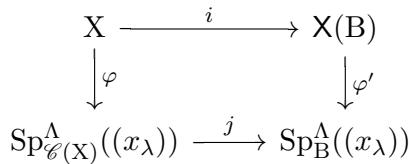
\includegraphics[keepaspectratio]{images/part001_f1662ccb.jpg}}

其中 \(\varphi\) 与 \(\varphi'\) 是由族 \((x_{\lambda})_{\lambda \in \Lambda}\) 所定义的映射（参见 I，第 41 页，第 6 节），而 \(i\) 与 \(j\) 是典范单射。则：

\begin{enumerate}
\def\labelenumi{\alph{enumi})}
\item
  映射 \(\varphi\) 与 \(\varphi'\) 是同胚；
\item
  联合谱 \(\mathrm{Sp}_{\mathrm{B}}^{\Lambda}((x_{\lambda}))\) 是 \(\mathrm{Sp}_{\mathcal{C}(\mathrm{X})}^{\Lambda}((x_{\lambda}))\) 的多项式凸包；
\item
  映射 \(\varphi\) 把 \(\mathcal{C}(\mathrm{X})\) 映为 \(\mathcal{C}(\mathrm{Sp}_{\mathcal{C}(\mathrm{X})}^{\Lambda}((x_{\lambda})))\) ，把 B 映为 \(\mathrm{P}(\mathrm{Sp}_{\mathcal{C}(\mathrm{X})}^{\Lambda}((x_{\lambda})))\) ；
\item
  映射 \(\varphi^{\prime}\) 把 \(\mathcal{G}_{\mathrm{B}}(\mathrm{B})\) 映为 \(\mathrm{P}(\mathrm{Sp}_{\mathrm{B}}^{\Lambda}((x_{\lambda})))\) ；
\item
  映射 \(\varphi\) 与 \(\varphi'\) 把 \(\mathcal{G}_{\mathrm{B}}\) 映为从 \(\mathrm{P}(\mathrm{Sp}_{\mathcal{C}(\mathrm{X})}^{\Lambda}((x_{\lambda})))\) 到 \(\mathrm{P}(\mathrm{Sp}_{\mathrm{B}}^{\Lambda}((x_{\lambda})))\) 上的典范同构。
\end{enumerate}

映射 \(\varphi\) 与 \(\varphi'\) 是连续且满射的（I，第 41 页，第 6 节）。映射 \(\varphi'\) 由 I，第 43 页，命题 12 的断言 \(a\) ）是同胚，且 \(i\) 是单射，因此 \(\varphi\) 是单射。于是 \(\varphi\) 与 \(\varphi'\) 都是同胚。

设 \(X_{1} = \mathrm{Sp}_{\mathcal{C}(X)}^{\Lambda}((x_{\lambda}))\) 。由 I，第 46 页，命题 14，\(X_{1}\) 的多项式凸包是 \(Y_{1} = \mathrm{Sp}_{\mathrm{B}}^{\Lambda}((x_{\lambda}))\) 。

对每个 \(\lambda\in\Lambda\) ，设 \(z_{\lambda}\) 是 \(\mathbf{C}^{\Lambda}\) 上相应的坐标函数。映射 \(\varphi\) 把 \(x_{\lambda}\) 映为 \(z_{\lambda}|X_{1}\) ，\(\varphi'\) 把 \(\mathcal{G}_{\mathrm{B}}(x_{\lambda})\) 映为 \(z_{\lambda}|Y_{1}\) 。因此 \(\varphi\) 把 B 映到 \(\mathrm{P}(X_{1})\) 上，\(\varphi'\) 把 \(\mathcal{G}_{\mathrm{B}}(B)\) 映到 \(\mathrm{P}(Y_{1})\) 上。最后，\(\varphi\) 与 \(\varphi'\) 把 \(\mathcal{G}_{\mathrm{B}}\) 映为从 \(\mathrm{P}(X_{1})\) 到 \(\mathrm{P}(Y_{1})\) 上的典范同构。

推论 1.　设 \(\Lambda\) 为一个集合，X 为 \(\mathbf{C}^{\Lambda}\) 的紧子集。我们把 X 等同于 \(\mathsf{X}(\mathrm{P}(\mathrm{X}))\) 的一个子集（I，第 142 页，命题 1，d)）。设 \((z_{\lambda})_{\lambda \in \Lambda}\) 为 \(\mathbf{C}^{\Lambda}\) 上坐标函数所成的族。

\begin{enumerate}
\def\labelenumi{\alph{enumi})}
\item
  映射 \(\theta\) 从 \(\mathrm{X}(\mathrm{P}(\mathrm{X}))\) 到 \(\mathrm{Sp}_{\mathrm{P}(\mathrm{X})}^{\Lambda}((z_{\lambda}))\) 上、由族 \((z_{\lambda})\) 所定义，它是从 \(\mathrm{X}(\mathrm{P}(\mathrm{X}))\) 到多项式凸包 \(Y\) （\(X\) 的多项式凸包）上的同胚。它在 \(X\) 上的限制是 \(X\) 的恒等映射；
\item
  对每个函数 \(f \in \mathrm{P}(\mathrm{X})\) ，同胚 \(\theta\) 把扩张 \(\mathcal{G}_{\mathrm{P}(\mathrm{X})}(f)\) （\(f\) 到 \(\mathrm{X}(\mathrm{P}(\mathrm{X}))\) 上的扩张）变换为扩张 \(\widetilde{f}\) （\(f\) 到 \(\mathrm{Y}\) 上的扩张）。映射 \(f \mapsto \widetilde{f}\) 是从 \(\mathrm{P}(\mathrm{X})\) 到 \(\mathrm{P}(\mathrm{Y})\) 上的典范同构。
\end{enumerate}

在命题 4 中取 B = P(X) 及 \(x_{\lambda} = z_{\lambda}\) 。则 \(\varphi\) 变成恒等映射，\(\varphi'\) 变成映射 \(\theta\) 。于是推论的断言就归结为同前处的断言。

推论 2.　设 \(\Lambda\) 为一个集合，\(X \subset \mathbf{C}^{\Lambda}\) 为紧集。若 \(X\) 连通，则它的多项式凸包连通。

若 X 连通，则 \(\mathcal{C}(\mathrm{X})\) 从而 \(\mathrm{P}(\mathrm{X})\) 的幂等元只有 0 和 1（I，第 79 页，命题的推论）。因此，空间 \(\mathrm{X}(\mathrm{P}(\mathrm{X}))\) 是连通的（同前）；而这个集合同胚于 X 的多项式凸包（推论 1，a)）。

\subsection{\texorpdfstring{\(C\) 的紧子集上的连续函数}{C 的紧子集上的连续函数}}

引理 1.　设 X 为平面的一个紧子集，O 为 \(\mathbf{C} - \mathbf{X}\) 的一个有界连通分支。则 O 的边界包含于 X。

集合 O 在 C−X 中的闭包等于 \(\overline{\mathrm{O}}\cap (\mathbf{C} - \mathbf{X})\) ，其中 \(\overline{\mathrm{O}}\) 是它在 C 中的闭包。由于 O 是 C−X 的一个连通分支，我们有 \(\overline{\mathrm{O}}\cap (\mathbf{C} - \mathbf{X}) = \mathrm{O}\) ，这确实证明了 \(\overline{\mathrm{O}} -\mathrm{O}\subset \mathrm{X}\) 。

设 X 为 C 的紧子集。设 \(O_{\infty}\) 为 \(\mathbf{C} - \mathbf{X}\) 的无界连通分支，\((\mathrm{O}_{i})_{i\in\mathrm{I}}\) 为 \(\mathbf{C} - \mathbf{X}\) 的有界连通分支的族，诸集合 \(O_{i}\) 两两不同。

设 E 为 \(\mathbf{C} - \mathbf{X}\) 的一个子集。我们用 \(\mathrm{R}_{\mathrm{E}}(\mathrm{X})\) 表示 \(\mathcal{C}(\mathrm{X})\) 中由函数 \(f|\mathrm{X}\) （其中 \(f\) 为 \(\mathbf{C}\) 上极点均属于 E 的有理函数）所成集合的闭包。代数 \(\mathrm{R}_{\mathrm{E}}(\mathrm{X})\) 是 \(\mathcal{C}(\mathrm{X})\) 的分离 X 的点的幺 Banach 子代数。设 z 是 X 上的恒等函数。\(\mathrm{R}_{\mathrm{E}}(\mathrm{X})\) 的由 z 生成的全闭子代数等于 \(\mathrm{R}_{\mathrm{E}}(\mathrm{X})\) （I，第 6 页，引理 2）。\(\mathrm{R}_{\mathrm{E}}(\mathrm{X})\) 的元素在 X 的内部全纯。

特别地，我们有 \(\mathrm{R}_{\varnothing}(\mathrm{X})=\mathrm{P}(\mathrm{X})\) 。我们记 \(\mathrm{R}(\mathrm{X})=\mathrm{R}_{\mathbf{C}-\mathbf{X}}(\mathrm{X})\) 。我们用 I(E) 表示这样的元素 \(i\in I\) 所成的集合：\(E\cap O_{i}=\varnothing\) ，并且

\[
\mathrm{X} _ {\mathrm{E}} = \mathrm{X} \cup \Big (\bigcup_ {i \in \mathrm{I} (\mathrm{E})} \mathrm{O} _ {i} \Big).
\]

集合 \(X_{E}\) 是紧的，因为它有界且闭：它在 \(\mathbf{C}\) 中的余集是开集 \(O_{\infty}\) 与诸和 E 相交的开集 \(O_{i}\) 的并。

命题 5.　沿用上述记号：

\begin{enumerate}
\def\labelenumi{\alph{enumi})}
\item
  从 \(\mathrm{R}_{\mathrm{E}}(\mathrm{X}_{\mathrm{E}})\) 到 \(\mathrm{R}_{\mathrm{E}}(\mathrm{X})\) 中的限制映射 h 是一个等距同构；
\item
  代数 \(\mathrm{R}_{\mathrm{E}}(\mathrm{X}_{\mathrm{E}})\) 是 \(\mathcal{C}(\mathrm{X}_{\mathrm{E}})\) 的全子代数；
\item
  \(\mathrm{R}_{\mathrm{E}}(\mathrm{X}_{\mathrm{E}})\) 的每个特征标都具有形式 \(f \mapsto f(w)\) ，其中 w 是 \(X_{E}\) 的元素；
\item
  映射 \(\chi \mapsto \chi (z)\) 是从 \(\mathsf{X}(\mathrm{R}_{\mathrm{E}}(\mathrm{X}))\) 到 \(\mathrm{X}_{\mathrm{E}}\) 上的同胚；
\item
  若 E′ 是 \(\mathbf{C} - \mathbf{X}\) 的子集，则我们有 \(\mathrm{R}_{\mathrm{E}}(\mathrm{X}) = \mathrm{R}_{\mathrm{E}'}(\mathrm{X})\) 当且仅当 \(\mathrm{X}_{\mathrm{E}} = \mathrm{X}_{\mathrm{E}'}\) ，这也等价于 \(\mathrm{I}(\mathrm{E}) = \mathrm{I}(\mathrm{E}')\) 。
\end{enumerate}

限制映射 \(h\) 从 \(\mathrm{R}_{\mathrm{E}}(\mathrm{X}_{\mathrm{E}})\) 到 \(\mathrm{R}_{\mathrm{E}}(\mathrm{X})\) 中，它是一个 Banach 代数态射，满足 \(\| h(f)\| \leqslant \| f\|\) 对每个函数 \(f\in \mathrm{R}_{\mathrm{E}}(\mathrm{X}_{\mathrm{E}})\) 成立。设 \(f\in \mathrm{R}_{\mathrm{E}}(\mathrm{X}_{\mathrm{E}})\) ，\(i\in \mathrm{I}(\mathrm{E})\) 。由于 \(f\) 在有界开集 \(\mathrm{O}_i\) 的一个邻域中全纯，最大模原理（VAR，I，第 29 页）蕴涵：存在元素 \(z_0\) ，它在 \(\mathrm{O}_i\) 的边界中，使得 \(|f(z_0)| = \sup_{z\in \mathrm{O}_i}|f(z)|\) 。由于 \(\mathrm{O}_i\) 的边界包含于 X（引理 1），由此得 \(\sup_{z\in \mathrm{O}_i}|f(z)|\leqslant \| h(f)\|\) 。由于这个不等式对每个 \(i\in \mathrm{I}(\mathrm{E})\) 成立，便得 \(\| f\| \leqslant \| h(f)\|\) 。因此态射 \(h\) 是等距的，特别地是单射。现在证明它是满射的。设 \(g\in \mathrm{R}_{\mathrm{E}}(\mathrm{X})\) 。存在极点都属于 E 的有理函数的序列 \((f_n)\) ，它在 X 上一致收敛于 \(g\) 。诸 \(f_n|\mathrm{X}_{\mathrm{E}}\) 是 \(\mathrm{R}_{\mathrm{E}}(\mathrm{X}_{\mathrm{E}})\) 的元素。由于 \(h\) 是等距的，序列 \((f_n|\mathrm{X}_{\mathrm{E}})\) 在 \(\mathcal{C}(\mathrm{X}_{\mathrm{E}})\) 中收敛。若 \(f\) 是它的极限，则我们有 \(f\in \mathrm{R}_{\mathrm{E}}(\mathrm{X}_{\mathrm{E}})\) 且 \(g = f|\mathrm{X} = h(f)\) 。由此得 \(a\) ）。

我们证明断言 d)。把 I，第 144 页，命题 3 应用于代数 \(B = \mathrm{R}_{\mathrm{E}}(\mathrm{X})\) 。同前处的断言 b) 蕴涵：把 \(\chi(z)\) 对应于 \(\chi\) 的映射是从 \(\mathsf{X}(\mathrm{R}_{\mathrm{E}}(\mathrm{X}))\) 到 \(\mathrm{Sp}_{\mathrm{R}_{\mathrm{E}}(\mathrm{X})}(z)\) 上的同胚。设 \(z_{\mathrm{E}}\) 为 \(\mathrm{X}_{\mathrm{E}}\) 的恒等映射。由同前处 a)，我们有 \(\mathrm{Sp}_{\mathrm{R}_{\mathrm{E}}(\mathrm{X})}(z) = \mathrm{Sp}_{\mathrm{R}_{\mathrm{E}}(\mathrm{X}_{\mathrm{E}})}(z_{\mathrm{E}})\) 。因此只需证明 \(\mathrm{Sp}_{\mathrm{R}_{\mathrm{E}}(\mathrm{X}_{\mathrm{E}})}(z_{\mathrm{E}}) = \mathrm{X}_{\mathrm{E}}\) 。I，第 28 页，命题 6 的推论表明，\(\mathrm{Sp}_{\mathrm{R}_{\mathrm{E}}(\mathrm{X}_{\mathrm{E}})}(z_{\mathrm{E}})\) 是 \(\mathrm{Sp}_{\mathcal{C}(\mathrm{X}_{\mathrm{E}})}(z_{\mathrm{E}}) = \mathrm{X}_{\mathrm{E}}\) 与 \(\mathrm{X}_{\mathrm{E}}\) 的余集的某些有界连通分支的并。设 \(\mathrm{O}_{i}\) 是 \(\mathrm{X}_{\mathrm{E}}\) 的余集的一个有界连通分支。则交 \(\mathrm{E} \cap \mathrm{O}_{i}\) 非空。设 \(\lambda \in \mathrm{E} \cap \mathrm{O}_{i}\) ；由于 \((\lambda - z_{\mathrm{E}})^{-1} \in \mathrm{R}_{\mathrm{E}}(\mathrm{X}_{\mathrm{E}})\) ，我们有 \(\lambda \notin \mathrm{Sp}_{\mathrm{R}_{\mathrm{E}}(\mathrm{X}_{\mathrm{E}})}(z_{\mathrm{E}})\) 。于是 \(\mathrm{O}_{i}\) 不包含于 \(\mathrm{Sp}_{\mathrm{R}_{\mathrm{E}}(\mathrm{X}_{\mathrm{E}})}(z_{\mathrm{E}})\) 。这就表明 \(\mathrm{Sp}_{\mathrm{R}_{\mathrm{E}}(\mathrm{X}_{\mathrm{E}})}(z_{\mathrm{E}}) = \mathrm{X}_{\mathrm{E}}\) 。

这个等式也蕴涵 \(\mathrm{Sp}_{\mathrm{R}_{\mathrm{E}}(\mathrm{X}_{\mathrm{E}})}(z_{\mathrm{E}})=\mathrm{Sp}_{\mathcal{C}(\mathrm{X}_{\mathrm{E}})}(z_{\mathrm{E}})\) 。这就建立了 I，第 41 页，命题 11 的条件 (iii)，该命题应用于 \(\mathrm{R}_{\mathrm{E}}(\mathrm{X}_{\mathrm{E}})\) 到 \(\mathcal{C}(\mathrm{X}_{\mathrm{E}})\) 中的典范单射以及元素 \(z_{\mathrm{E}}\) 。断言 b) 与 c) 就是同前处的等价条件 (i) 与 (ii)。

断言 \(d\) ）表明 \(\mathrm{X}_{\mathrm{E}} = \mathrm{X}_{\mathrm{E}'}\) ，只要 \(\mathrm{R}_{\mathrm{E}}(\mathrm{X}) = \mathrm{R}_{\mathrm{E}'}(\mathrm{X})\) 成立。反之，假设 \(\mathrm{X}_{\mathrm{E}} = \mathrm{X}_{\mathrm{E}'}\) 。把 \(\mathrm{E}'\) 换成 \(\mathrm{E} \cup \mathrm{E}'\) ，我们就可以假设 \(\mathrm{E} \subset \mathrm{E}'\) 。根据 \(b\) ），代数 \(\mathrm{R}_{\mathrm{E}}(\mathrm{X}_{\mathrm{E}})\) 是 \(\mathcal{C}(\mathrm{X}_{\mathrm{E}})\) 的全闭子代数，因而也是 \(\mathrm{R}_{\mathrm{E}'}(\mathrm{X}_{\mathrm{E}})\) 的全闭子代数。它包含 \(z_{\mathrm{E}}\) ，从而 \(\mathrm{R}_{\mathrm{E}}(\mathrm{X}_{\mathrm{E}}) = \mathrm{R}_{\mathrm{E}'}(\mathrm{X}_{\mathrm{E}})\) 。应用 \(a\) ），便推出 \(\mathrm{R}_{\mathrm{E}}(\mathrm{X}) = \mathrm{R}_{\mathrm{E}'}(\mathrm{X})\) 。最后，\(\mathrm{X}_{\mathrm{E}} = \mathrm{X}_{\mathrm{E}'}\) 与 \(\mathrm{I}(\mathrm{E}) = \mathrm{I}(\mathrm{E}')\) 的等价性是定义的直接推论。

推论 1.　下列条件等价：

\begin{enumerate}
\def\labelenumi{(\roman{enumi})}
\item
  集合 E 与 \(\mathbf{C} - \mathbf{X}\) 的每个有界连通分支相交；
\item
  映射 \(\chi \mapsto \chi (z)\) 是从 \(\mathsf{X}(\mathrm{R}_{\mathrm{E}}(\mathrm{X}))\) 到 \(\mathrm{X}\) 上的同胚；
\item
  我们有 \(\mathrm{R_E(X)} = \mathrm{R(X)}\) 。
\end{enumerate}

设 \(E' = \mathbf{C} - \mathbf{X}\) 。条件 (i)、(ii)、(iii) 分别等价于 \(\mathrm{I}(\mathrm{E}) = \mathrm{I}(\mathrm{E}')\) 、等价于 \(\mathrm{X}_{\mathrm{E}} = \mathrm{X}_{\mathrm{E}'}\) （由命题 5，d)）、等价于 \(\mathrm{R}_{\mathrm{E}}(\mathrm{X}) = \mathrm{R}_{\mathrm{E}'}(\mathrm{X})\) 。因此，由命题 5，e)，它们彼此等价。

下面的推论使 Runge 定理（I，第 69 页，定理 3）更精确。

推论 2（Runge 定理）.　对每个 \(i \in I\) ，设 \(\lambda_{i}\) 为 \(O_{i}\) 中的一点。设 f 为在 X 的一个开邻域中全纯的复函数。则 \(f|X\) 是极点取自诸 \(\lambda_{i}\) 的有理函数的限制在 X 上的一致极限。

取 \(E = \{\lambda_{i}\}_{i \in I}\) ，假设便是推论 1 的条件 (i)。因此我们有 \(\mathrm{R}_{\mathrm{E}}(\mathrm{X}) = \mathrm{R}(\mathrm{X})\) ，而 I，第 69 页，定理 3 表明 \(\mathrm{R}(\mathrm{X}) = \mathcal{O}(\mathrm{X})\) 。

\exercisesection{谱与特征标}


\begin{enumerate}
\def\labelenumi{\arabic{enumi})}
\item
  设 \((e_{1}, e_{2})\) 为 \(R^{2}\) 的典范基，u 为 A = \(\mathcal{L}(\mathbf{R}^{2})\) 中由 \(u(e_{1}) = e_{2}\) ，\(u(e_{2}) = -e_{1}\) 所定义的元素。证明 \(\mathrm{Sp}_{\mathrm{A}}(u) = \varnothing\) 与 \(\mathrm{Sp}_{\mathrm{A}}(u^{2}) = \{-1\}\) 。
\item
  设 \(\mu\) 为 \([0,1]\) 上的 Lebesgue 测度，H 为 Hilbert 空间 \(\mathrm{L}_{\mathbf{C}}^{2}([0,1],\mu)\) ，\(\mathrm{A} = \mathcal{L}(\mathrm{H})\) ，\(x \in \mathrm{A}\) 为把函数 \(f(t)\) 变换为函数 \(tf(t)\) 的算子。证明 \(\mathrm{Sp}_{\mathrm{A}}(x) = [0,1]\) ，但 \(x\) 没有特征值。
\item
  \begin{enumerate}
  \def\labelenumii{\alph{enumii})}
  \tightlist
  \item
    设 H 为具有可数正交基 \((e_{0}, e_{1}, e_{2}, \ldots)\) 的 Hilbert 空间，A = L(H)。设 \(u \in \mathcal{L}(H)\) 满足：对每个 i 有 \(u(e_{i}) = e_{i+1}\) 。设 \(u' \in \mathcal{L}(H)\) 满足：\(u'(e_{i}) = e_{i-1}\) 对 \(i \geqslant 1\) 成立，且 \(u'(e_{0}) = 0\) 。我们有 \(u'u = 1\) ，但 \(uu'(e_{0}) = 0\) ，于是 \(\mathrm{Sp}_{\mathrm{A}}(u'u) \neq \mathrm{Sp}_{\mathrm{A}}(uu')\) 。
  \end{enumerate}
\end{enumerate}

\begin{enumerate}
\def\labelenumi{\alph{enumi})}
\setcounter{enumi}{1}
\tightlist
\item
  设 A 为交换域上的幺 Noether 代数。若 \(x, y \in A\) ，则有 \(\mathrm{Sp}_{\mathrm{A}}(xy) = \mathrm{Sp}_{\mathrm{A}}(yx)\) （利用 A，VIII，第 37 页，习题 6）。
\end{enumerate}

\begin{enumerate}
\def\labelenumi{\arabic{enumi})}
\setcounter{enumi}{3}
\tightlist
\item
  设 A 为 C 上的交换代数，I 为 A 的理想，h 为 I 到 A 中的典范单射，S 为在 I 上为零的 \(\chi \in \mathsf{X}'(\mathsf{A})\) 所成的集合。
\end{enumerate}

\begin{enumerate}
\def\labelenumi{\alph{enumi})}
\item
  \(X'(h)\) 是满射的。
\item
  \(\mathsf{X}^{\prime}(h)|(\mathsf{X}^{\prime}(\mathsf{A})-\mathsf{S})\) 是从 \(\mathsf{X}^{\prime}(\mathsf{A})-\mathsf{S}\) 到 \(\mathsf{X}(\mathsf{I})\) 上的同胚。（设 \(\chi_{0}\in\mathsf{X}^{\prime}(\mathsf{A})-\mathsf{S}\) 。设 \(x_{1},\ldots,x_{n}\in\mathsf{A}\) ，\(\varepsilon>0\) ，并设 V 为 \(\chi_{0}\) 在 \(\mathsf{X}^{\prime}(\mathsf{A})\) 中由 \(|(\chi-\chi_{0})(x_{i})|\leqslant\varepsilon,(i=1,\ldots,n)\) 所定义的邻域。设 \(u_{0}\in I\) 满足 \(\chi_0(u_0) = 1\) 。我们有 \(u_i = u_0x_i \in I\) 。于是，若 \(|(\chi - \chi_0)(u_i)| \leqslant \delta\) （ \(i = 0, 1, \ldots, n\) ），其中 \(\delta\) 足够小，则我们有 \(\chi \in V\) 。）
\end{enumerate}

\begin{enumerate}
\def\labelenumi{\arabic{enumi})}
\setcounter{enumi}{4}
\item
  在习题 4 中，取 \(A = \mathbf{C}[X,Y]\) 与 \(I = AX\) 。空间 X(A) 等同于 \(\mathbf{C}^2\) ，S = \{0\} 等同于 \(\{0\} \times \mathbf{C}\) 。设 U 为这样的 \((\xi, \eta) \in \mathbf{C}^2\) 所成的集合：\(|\xi| < e^{-|\eta|}\) 。证明 \(X'(h)(U)\) 不是 0 在 \(X'(I)\) 中的邻域。由此推出，\(X'(I)\) 不能等同于 \(X'(A)\) 关于由 \(X'(h)\) 所定义的等价关系的商空间。（关于这一主题，参见 I，第 169 页，习题 17。）
\item
  设 A 为域上的交换代数，I 为 A 的极大理想。证明我们有 \(A^{2} \subset I\) 且 \(\dim(A/I) = 1\) ，或者 A/I 是一个域。（对 A/I 应用 A，I，第 153 页，习题 3。）特别地，若 \(A^{2} = A\) ，则 A 的每个极大理想都是正则的。
\item
  设 A 为交换域 K 上的交换代数，\(x \in A\) ，\(\alpha \in K\) 。这样的 \(\chi \in \mathsf{X}(\mathsf{A})\) 所成的集合：\((\mathcal{G}x)(\chi) = \alpha\) ，它在 Jacobson 拓扑下是闭的。（先归结为 A 有单位元的情形，再归结为 \(\alpha = 0\) 的情形。）
\end{enumerate}

¶ 8) 设 A 为一个代数，I 为 A 的双边理想，\(\mathrm{J}^{\mathrm{I}}(\mathrm{A})\) 为 A 的不包含 I 的本原理想所成的集合，\(\widehat{A}^{I}\) 为不可约表示 \(\pi \in \widehat{A}\) （满足 \(\pi(I) \neq 0\) ）所成的集合。

\begin{enumerate}
\def\labelenumi{\alph{enumi})}
\item
  若 \(\pi \in \widehat{\mathrm{A}}^{\mathrm{I}}\) ，则 \(\pi | \mathrm{I} \in \widehat{\mathrm{I}}\) （I，第 12 页，引理 5，\(a\) ））。若表示 \(\pi\) 与 \(\pi' \in \widehat{\mathrm{A}}\) 使得 \(\pi | \mathrm{I}\) 与 \(\pi'|\mathrm{I}\) 等价，则 \(\pi\) 与 \(\pi'\) 等价。（可以假设 \(\pi(x) = \pi'(x)\) 对所有 \(x \in \mathrm{I}\) 成立。于是，对每个 \(y \in \mathrm{A}\) ，\(\pi(y)\) 与 \(\pi'(y)\) 在 \(\sum_{x \in \mathrm{I}} \operatorname{Im} \pi(x)\) 上一致，而这个子空间等于 \(\pi\) 的空间。）
\item
  若 \(\pi \in \widehat{\mathrm{I}}\) ，则 \(\pi\) 可扩张为 \(\widehat{\mathrm{A}}^{\mathrm{I}}\) 的一个元素。（设 R 为 I 的极大正则左理想。设 \(g\) 为 I 模 R 的右单位元。假设 A 有单位元，证明关系式 \(\mathrm{AR} + \mathrm{A}(1 - g) = \mathrm{A}\) 将导出 \(g^2 \in \mathrm{R}\) 。因此 \(\mathrm{AR} + \mathrm{A}(1 - g)\) 包含于 A 的一个极大左理想 M。证明 \(\mathrm{M} \cap \mathrm{I} = \mathrm{R}\) 与 \(\mathrm{M} + \mathrm{I} = \mathrm{A}\) 。）
\item
  由 a) 与 b) 推出：映射 \(I'\mapsto I'\cap I\) 是从 \(\mathrm{J}^{\mathrm{I}}(\mathrm{A})\) 到 \(\mathrm{J}(\mathrm{I})\) 上的同胚，且映射 \(\pi\mapsto\pi|I\) 是从 \(\widehat{A}^{I}\) 到 \(\widehat{I}\) 上的同胚。
\end{enumerate}

\exercisesection{赋范代数}

\begin{enumerate}
\def\labelenumi{\arabic{enumi})}
\tightlist
\item
  设 (A, e) 为一个复幺代数。
\end{enumerate}

\begin{enumerate}
\def\labelenumi{\alph{enumi})}
\tightlist
\item
  对于线性型 \(\lambda \in \mathrm{A}^*\)，当 \(\lambda(e) = 1\) 时，下列条件等价：
\end{enumerate}

\begin{enumerate}
\def\labelenumi{(\roman{enumi})}
\item
  对每个 \(x \in \operatorname{Ker}(\lambda)\)，有 \(x^2 \in \operatorname{Ker}(\lambda)\)；
\item
  对每个 \(x \in \mathbb{A}\)，有 \(\lambda(x^{2}) = \lambda(x)^{2}\)；
\item
  \(\lambda\) 的核是 A 的一个右理想；
\item
  线性型 \(\lambda\) 是从 A 到 C 的保单位元态射。
\end{enumerate}

（注意 \(\lambda(x - \lambda(x)e) = 0\) 对所有 \(x\in A\) 成立。）

\begin{enumerate}
\def\labelenumi{\alph{enumi})}
\setcounter{enumi}{1}
\item
  设 \(\lambda \in \mathrm{A}^*\) 为满足 \(\lambda(1) = 1\) 的线性型，且使得对每个 \(x \in \mathrm{A}\)，有 \(\lambda(x) \in \mathrm{Sp}_{\mathrm{A}}(x)\)。设 \(x \in \mathrm{Ker}(\lambda)\) 满足 \(\lambda(x^{2}) \neq 0\)，则 \(x\) 的谱在 \(\mathbf{C}\) 中无界。（取整数 \(n \geqslant 2\)，考虑多项式 \(p \in \mathbf{C}[\mathrm{X}]\)，使 \(p(z) = \lambda((ze - x)^{n})\) 对所有 \(z \in \mathbf{C}\) 成立；注意它的根都属于 \(x\) 的谱，并用 \(|\lambda(x^{2})|\) 给出它们的欧氏范数的下界。）
\item
  假设 A 是 Banach 代数。为使 A 上的线性型 \(\lambda\) 是从 A 到 C 的保单位元态射，充要条件是 \(\lambda(e)=1\)，且 \(\lambda(x)\in\mathrm{Sp}_{\mathrm{A}}(x)\) 对所有 \(x\in A\) 成立。
\end{enumerate}

\begin{enumerate}
\def\labelenumi{\arabic{enumi})}
\setcounter{enumi}{1}
\tightlist
\item
  设 \(n \geqslant 0\) 为整数。设 \(A_n\) 为由函数 \(f: [0,1] \to \mathbf{C}\)（它在 \([0,1]\) 上具有直到 \(n\) 阶的连续导数）所组成的交换复 Banach 代数，赋以范数
\end{enumerate}

\[
\| f \| = \sum_ {k = 0} ^ {n} \frac {1}{k !} \sup _ {0 \leqslant t \leqslant 1} | f ^ {(k)} (t) |
\]

（I，第 18 页，例 4）。证明 \(A_{n}\) 同构于 \(A_{m}\) 当且仅当 n = m。（不过，根据 I，第 144 页，例 1，这些 Banach 代数都有相同的特征标空间。）

\begin{enumerate}
\def\labelenumi{\arabic{enumi})}
\setcounter{enumi}{2}
\tightlist
\item
  设 G 为等于其导出子群的群（A，I，第 67 页）。对每个 \(g \in G\)，用 \(\ell(g)\) 表示满足下列条件的最小整数 \(k \geqslant 0\)：存在数对 \((a_{1}, b_{1}), \ldots, (a_{k}, b_{k})\)（取自 \(G \times G\)），使 \(g = [a_{1}, b_{1}] \cdots [a_{k}, b_{k}]\)。
\end{enumerate}

\begin{enumerate}
\def\labelenumi{\alph{enumi})}
\item
  映射 \(\ell\) 是 G 上的一个度量。
\item
  对每个 \(g \in \mathbf{G}\)，极限
\end{enumerate}

\[
\operatorname{lsc} (g) = \lim _ {n \to + \infty} \frac {\ell (g ^ {n})}{n}
\]

存在，称为 g 的稳定换位子长度。

\begin{enumerate}
\def\labelenumi{\alph{enumi})}
\setcounter{enumi}{2}
\tightlist
\item
  设 S 为一个集合，\(\mathrm{G} = \mathrm{D}(\mathrm{F}(\mathrm{S}))\) 为由 S 生成的自由群的导出子群。群 G 等于其导出子群，且对每个 \(g \in G\)，\(g \neq e\)，有 \(\operatorname{lsc}(g) \geqslant 1/2\)。存在 \(g \in G\) 使 \(\operatorname{lsc}(g) = 1/2\)。
\end{enumerate}

\begin{enumerate}
\def\labelenumi{\arabic{enumi})}
\setcounter{enumi}{3}
\tightlist
\item
  设 \(n \geqslant 1\) 为整数。用 \(S(n)\) 表示满足下列条件的最大整数 \(k \geqslant 0\)：对每个集合 \(X\)（由 \(n\) 个实数组成），存在子集 \(Y \subset X\)（基数为 \(k\)），使方程 \(x + y = z\) 在 \(Y\) 中无解。于是 \(S(n) \leqslant n\)。
\end{enumerate}

\begin{enumerate}
\def\labelenumi{\alph{enumi})}
\tightlist
\item
  证明极限
\end{enumerate}

\[
\sigma = \lim _ {n \to + \infty} \frac {\mathrm{S} (n)}{n}
\]

存在。

\begin{enumerate}
\def\labelenumi{\alph{enumi})}
\setcounter{enumi}{1}
\item
  证明 \(\sigma \leqslant 2 / 5\)。
\item
  证明 \(\sigma \geqslant 1 / 3\)。
\end{enumerate}

（可以证明 \(\sigma = 1/3\)，参见 S. EBERHARD, B. GREEN, F. MANNERS, Sets of integers with no large sum-free subset, Annals of Mathematics 180 (2014), 621--652。）

\begin{enumerate}
\def\labelenumi{\arabic{enumi})}
\setcounter{enumi}{4}
\tightlist
\item
  设 A 为交换环，\(n \geqslant 1\) 为整数。对于系数在 A 中的矩阵 \(M = (m_{i,j})\)（其型为 \((n, n)\)），我们把 M 的积和式称为元素
\end{enumerate}

\[
\mathrm{per(M)} = \sum_ {\sigma \in \mathrm{S} _ {n}} m _ {1, \sigma (1)} \dots m _ {n, \sigma (n)}
\]

该元素属于 A。

设 \(k \geqslant 1\) 为整数。用 \(X_{n,k}\) 表示由实系数的、型为 \((n, n)\) 且每列恰含 k 个等于 1 的系数（其余系数全为零）的矩阵 M 所成的集合。

证明极限

\[
\lim _ {n \to + \infty} \left(\inf _ {\mathrm{M} \in \mathrm{X} _ {n, k}} \operatorname{per} (\mathrm{M})\right) ^ {1 / n}
\]

存在。

\begin{enumerate}
\def\labelenumi{\arabic{enumi})}
\setcounter{enumi}{5}
\tightlist
\item
  设 \(k \geqslant 1\) 为整数。对每个整数 \(N \geqslant 1\)，用 \(S_k(N)\) 表示不包含 \(A \subset \{1, \ldots, N\}\) 个成等差数列的元素的集合 \(k\) 的最大基数；也就是说，对任意 \(n_0 \geqslant 0\)、\(h \geqslant 1\)、\(\ell \geqslant 1\)，若 \(\{n_0 + h, n_0 + 2h, \ldots, n_0 + \ell h\} \subset A\)，则 \(\ell < k\)。
\end{enumerate}

\begin{enumerate}
\def\labelenumi{\alph{enumi})}
\tightlist
\item
  证明极限
\end{enumerate}

\[
s _ {k} = \lim _ {\mathrm{N} \to + \infty} \frac {\mathrm{S} _ {k} (\mathrm{N})}{\mathrm{N}}
\]

存在。

\begin{enumerate}
\def\labelenumi{\alph{enumi})}
\setcounter{enumi}{1}
\tightlist
\item
  证明 \(s_{1}=s_{2}=0\)。可以证明（“Szemerédi 定理”，参见 E. SZEMERÉDI, On sets of integers containing no k elements in arithmetic progression, Acta Arithmetica XXVII, 1975, 199--245）：对所有 \(s_{k}=0\) 有 \(k\geqslant1\)；至于 k=3 的情形，参见 II，第 270 页，习题 23。
\end{enumerate}

\begin{enumerate}
\def\labelenumi{\arabic{enumi})}
\setcounter{enumi}{6}
\tightlist
\item
  设 A 为赋范代数。
\end{enumerate}

\begin{enumerate}
\def\labelenumi{\alph{enumi})}
\tightlist
\item
  设 S 为 A 的非空有界子集。证明极限
\end{enumerate}

\[
\varrho (\mathrm{S}) = \lim _ {n \to + \infty} \sup _ {x \in \mathrm{S} ^ {n}} \| x \| ^ {1 / n}
\]

存在，并且当 S 仅由单个元素 x 组成时，有 \(\varrho(\mathrm{S}) = \varrho(x)\)。我们称 \(\varrho(\mathrm{S})\) 为子集 S 的谱半径。

\begin{enumerate}
\def\labelenumi{\alph{enumi})}
\setcounter{enumi}{1}
\tightlist
\item
  设 N 为 A 上与 A 的范数等价、且使赋以 p 之后的 A 仍为赋范代数的范数 p 全体所成的集合。设 X 为 A 的一个子集。为存在 \(p \in N\) 使得对所有 \(p(x) \leqslant 1\) 都有 \(x \in X\)，充要条件是存在实数 \(c \geqslant 0\) 使得
\end{enumerate}

\[
\sup _ {n \geqslant 1} \sup _ {x \in X ^ {n}} \| x \| \leqslant c.
\]

\begin{enumerate}
\def\labelenumi{\alph{enumi})}
\setcounter{enumi}{2}
\tightlist
\item
  证明
\end{enumerate}

\[
\varrho (\mathrm{S}) = \inf _ {p \in \mathrm{N}} \sup _ {x \in \mathrm{S}} p (x).
\]

\begin{enumerate}
\def\labelenumi{\arabic{enumi})}
\setcounter{enumi}{7}
\item
  设 A 为 \(\mathbf{R}\) 上在无穷远处趋于 0 的复值连续函数所成的代数，赋以范数 \(\|f\| = \sup_{t\in\mathbf{R}} |f(t)|\)。于是 \(\widetilde{\mathrm{A}}\) 就恒同于 \(\mathbf{R}\) 上在无穷远处趋于有限极限的复值连续函数所成的代数。在 \(\widetilde{\mathrm{A}}\) 上，范数 \(\|g\| = \sup_{t\in\mathbf{R}} |g(t)|\) 与 I，第 15 页，第 1 节中定义的范数不同。
\item
  设 A 为赋范代数，\(b = \inf_{x \neq 0} \|x^{2}\|/\|x\|^{2}\)。则
\end{enumerate}

\[
b \leqslant \inf _ {x \neq 0} \frac {\varrho (x)}{\| x \|} \leqslant \sqrt {b}.
\]

\begin{enumerate}
\def\labelenumi{\arabic{enumi})}
\setcounter{enumi}{9}
\item
  设 A 为赋范代数，\(x, y \in A\)。我们有 \(\varrho(xy) = \varrho(yx)\)。
\item
  设 H 为可数型 Hilbert 空间，\((f_{n})_{n\geqslant1}\) 为 H 的一个标准正交基。设 A 为赋范代数 \(\mathcal{L}(\mathrm{H})\)。设 \(x\in A\) 为由 \(x(f_{i})=2^{-i}f_{i+1}\) 所定义的元素。证明 x 是拟幂零元，但不是幂零元。
\end{enumerate}

\begin{enumerate}
\def\labelenumi{¶ \arabic{enumi})}
\setcounter{enumi}{11}
\tightlist
\item
  设 H 为可分 Hilbert 空间，\((f_n)_{n \geqslant 1}\) 为 H 的一个标准正交基。按下述方式定义诸数 \((\alpha_m)_{m \geqslant 1}\)：若 \(\alpha_m = e^{-k}\) 是 \(m\) 与一个奇数之积，则令 \(2^k\)。
\end{enumerate}

\begin{enumerate}
\def\labelenumi{\alph{enumi})}
\tightlist
\item
  设 \(x \in \mathcal{L}(\mathrm{H})\) 由 \(x(f_m) = \alpha_m f_{m+1}\)（对所有 \(m \geqslant 1\)）定义。证明 \(x\) 不是拟幂零元。（注意
\end{enumerate}

\[
\left\| x ^ {n} \right\| = \sup _ {m} \bigl (\alpha_ {m} \alpha_ {m + 1} \dots \alpha_ {m + n - 1} \bigr),
\]

并估计 \(\alpha_{1}\alpha_{2}\ldots\alpha_{2^{t}-1}\)。）

\begin{enumerate}
\def\labelenumi{\alph{enumi})}
\setcounter{enumi}{1}
\tightlist
\item
  设 \(x_{k} \in \mathcal{L}(\mathrm{H})\) 由下式定义：当 m 是 \(x_{k}(f_{m}) = 0\) 与一个奇数之积时 \(2^{k}\)，否则 \(x_{k}(f_{m}) = \alpha_{m} f_{m+1}\)。证明 \(x_{k}\) 是幂零元，且当 k 趋于 \((x_{k})\) 时 \(+\infty\) 收敛于 x。
\end{enumerate}

\begin{enumerate}
\def\labelenumi{\arabic{enumi})}
\setcounter{enumi}{12}
\item
  设 A 为幺 Banach 代数。设 \(x \in A\) 满足 \(\|x - 1\| < 1\)。则存在 \(y \in A\) 使 \(y^{2} = x\)。
\item
  设 A 为复幺赋范代数。若对 A 的每个可逆元 x 都有 \(\|x^{-1}\| = \|x\|^{-1}\)，则 A = C · 1。（可归结为 A 完备的情形。设 \(x \in A\) 与 C · 1 的距离为 \(\alpha > 0\)。若 \(\lambda_{0} \in C\) 使 \(x - \lambda_{0}\) 可逆，则当 \(x - \lambda\) 时 \(|\lambda - \lambda_{0}| < \alpha\) 也必可逆。由此推出 x 的谱将是空集。）
\item
  设 A 为复幺赋范代数，其中仅有的左拓扑零因子是 0，仅有的右拓扑零因子也是 0。则 \(A = C \cdot 1\)。（若 \(x \in A\)，且 \(\lambda\) 属于 \(\mathrm{Sp}_{\widehat{\mathrm{A}}}(\boldsymbol{x})\) 的边界，则 \(x - \lambda\) 是 \(\widehat{A}\) 中的拓扑零因子，因而是 A 中的拓扑零因子，于是 \(x = \lambda\)。）
\item
  设 A 为复幺 Banach 代数。设 \(a\) 为 A 的一个元素。我们把 a 的奇异谱称为满足下列条件的 \(\lambda \in \mathbf{C}\) 所成的集合：\(a - \lambda e\) 在 A 中既是左拓扑零因子又是右拓扑零因子。
\end{enumerate}

\begin{enumerate}
\def\labelenumi{\alph{enumi})}
\item
  证明 a 的奇异谱包含于 a 的谱中，并且包含 a 的谱的边界。
\item
  设 \(f \in C[X]\) 为多项式。a 的奇异谱在 f 下的像就是 \(f(a)\) 的奇异谱。
\end{enumerate}

\begin{enumerate}
\def\labelenumi{\arabic{enumi})}
\setcounter{enumi}{16}
\tightlist
\item
  对每个 \(x \in A\)，我们令：
\end{enumerate}

\[
\lambda (x) = \inf _ {y \neq 0} \frac {\| x y \|}{\| y \|} \quad \lambda^ {\prime} (x) = \inf _ {y \neq 0} \frac {\| y x \|}{\| y \|}.
\]

\begin{enumerate}
\def\labelenumi{\alph{enumi})}
\tightlist
\item
我们有
\end{enumerate}

\[
| \lambda (x) - \lambda (y) | \leqslant \| x - y \|, \quad | \lambda^ {\prime} (x) - \lambda^ {\prime} (y) | \leqslant \| x - y \|,
\]

\[
\lambda (x) \lambda (y) \leqslant \lambda (x y) \leqslant \| x \| \lambda (y), \quad \lambda^ {\prime} (x) \lambda^ {\prime} (y) \leqslant \lambda^ {\prime} (x y) \leqslant \lambda^ {\prime} (x) \| y \|.
\]

\begin{enumerate}
\def\labelenumi{\alph{enumi})}
\setcounter{enumi}{1}
\tightlist
\item
  A 中的左（相应地，右）拓扑零因子所成的集合是闭集。
\end{enumerate}

\begin{enumerate}
\def\labelenumi{\arabic{enumi})}
\setcounter{enumi}{17}
\item
  设 A 为幺 Banach 代数。由既不可逆又不是拓扑零因子的 \(x\) 所成的集合在 A 中是开集。
\item
  设 X 为复 Banach 空间，\(x \in A = \mathcal{L}(X)\)。
\end{enumerate}

\begin{enumerate}
\def\labelenumi{\alph{enumi})}
\tightlist
\item
  若 x 不可逆，则 x 是左拓扑零因子或右拓扑零因子。（依次考虑下列各种情形：）
\end{enumerate}

\(1^{\circ}\) ) \(x\) 不是单射；

\(2^{\circ})\overline{x(\mathrm{X})}\neq \mathrm{X};\)

\(3^{\circ}) x \text{ 是单射的， } x(\mathrm{X}) \text{ 在 X 中稠密且不同于 X。}\)

\begin{enumerate}
\def\labelenumi{\alph{enumi})}
\setcounter{enumi}{1}
\tightlist
\item
  若 x 把 X 双连续地映到 X 的一个异于 X 的闭向量子空间上，或者 x 非单射而其像为 X，则 x 位于 A 的不可逆元素所成集合的内部。
\end{enumerate}

\begin{enumerate}
\def\labelenumi{\arabic{enumi})}
\setcounter{enumi}{19}
\item
  在 I，第 20 页，例 9 的代数 A 中，恒等函数 z 既不可逆，也不是拓扑零因子。
\item
  设 A 为幺赋范代数。设 B 为赋范代数 \(\mathcal{L}(\mathrm{A})\)。于是 A 在态射 \(x \mapsto \gamma_x\) 下的像是 B 的一个全子代数。因此，若 \(x \in \mathrm{A}\)，则 \(\mathrm{Sp}_{\mathrm{A}}(x) = \mathrm{Sp}_{\mathrm{B}}(\gamma_x)\)。
\end{enumerate}

\begin{enumerate}
\def\labelenumi{¶ \arabic{enumi})}
\setcounter{enumi}{21}
\tightlist
\item
  设 A 为 Banach 代数。
\end{enumerate}

\begin{enumerate}
\def\labelenumi{\alph{enumi})}
\tightlist
\item
  设 S 为由 A 的元素组成的有界序列全体，赋以范数 \(\|(\boldsymbol{x}_{n})\| = \sup \|x_{n}\|\)。设 R 为 \((x_{n}) \in \mathrm{S}\) 中使得 \(\|x_{n}\|\) 趋于 0 的元素所成的集合。于是 S 是 Banach 代数，而 R 是 S 的一个闭双边理想。
\end{enumerate}

设 \(S' = \text{S/R}\)，并设 \(\varphi: \text{S} \to \text{S}'\) 为典范同态。

\begin{enumerate}
\def\labelenumi{\alph{enumi})}
\setcounter{enumi}{1}
\item
  映射 \(\theta\)（由 \(\theta(x) = \varphi(x, x, x, \ldots)\) 定义，从 A 到 S' 中）是 A 到 S' 的一个子代数上的等距同构。S' 中的每个左拓扑零因子都是左零因子。为使 \(x \in A\) 是左拓扑零因子，充要条件是 \(\theta(x)\) 是 S' 中的左零因子。
\item
  假设 A 有单位元。证明：存在一个 Banach 代数 B 以及 A 到 B 的一个子代数上的等距同构，使得 A 的元素不可逆当且仅当它在 B 中的像是左零因子或右零因子。（利用 a) 以及习题 19 与 21。）
\end{enumerate}

\begin{enumerate}
\def\labelenumi{\arabic{enumi})}
\setcounter{enumi}{22}
\tightlist
\item
  设 A 为赋范代数，R 为其根。
\end{enumerate}

\begin{enumerate}
\def\labelenumi{\alph{enumi})}
\item
  若 \(x \in R\)，则 x 是拟幂零元。（我们有 \(\mathrm{Sp}_{\mathrm{A}}^{\prime}(x) = \{0\}\)，从而更有 \(\mathrm{Sp}_{\widehat{\mathrm{A}}}^{\prime}(x) = \{0\}\)。）
\item
  假设 A 是 Banach 代数。设 I 为 A 的一个左理想，其所有元素都是拟幂零元。则 \(I \subset R\)（可以假设 A 有单位元。若 \(x \in R\) 且 \(a \in A\)，则有 \(\mathrm{Sp}_{\mathrm{A}}(ax) = \{0\}\)，因而 1 - ax 可逆；从而 \(x \in R\)。
\end{enumerate}

\begin{enumerate}
\def\labelenumi{\arabic{enumi})}
\setcounter{enumi}{23}
\item
  设 A 为复 Banach 代数，B 为无根的复代数，\(\varphi\) 为从 A 到 B 上的态射。\(\varphi\) 的核是闭的。
\item
  设 A 为复 Banach 代数，\(\pi\) 为 A 在复向量空间 X 中的一个非零不可约表示。设 \(\xi_{0}\) 为 X 的非零元素。
\end{enumerate}

\begin{enumerate}
\def\labelenumi{\alph{enumi})}
\item
  \(\xi_0\) 的零化子 I 是 A 的一个正则极大左理想；它是闭的。
\item
  映射 \(x \mapsto x\xi_{0}\) 通过过渡到商，定义了 A-模 A/I 到 A-模 X 上的一个同构 \(\varphi\)。
\item
  若经 \(\varphi\) 把 Banach 空间 A/I 的范数转移过来，则 X 成为 Banach 空间，且对所有 \(\| \pi (x)\| \leqslant \| x\|\) 有 \(x\in \mathrm{A}\)。
\item
  若 A 是本原的（即 \(\{0\}\) 是本原理想，参见 I，第 11 页的定义，另参见 A，VIII，第 433 页，习题 6），则依照 A 有或没有单位元而分别有 \(A = \{0\}\) 或 \(C \cdot 1\)。（利用前面的结果以及 I，第 26 页的推论 4。）
\end{enumerate}

\begin{enumerate}
\def\labelenumi{¶ \arabic{enumi})}
\setcounter{enumi}{25}
\tightlist
\item
  设 A 为 Banach 代数，R 为其根。
\end{enumerate}

\begin{enumerate}
\def\labelenumi{\alph{enumi})}
\tightlist
\item
  证明：若 \(r \in R\)，则级数
\end{enumerate}

\[
- \frac {1}{2} \sum_ {k = 1} ^ {\infty} \binom{1 / 2}{k} (- 4 r) ^ {k}
\]

收敛于满足 \(x \in R\) 的元素 \(x^{2} - x + r = 0\)。

\begin{enumerate}
\def\labelenumi{\alph{enumi})}
\setcounter{enumi}{1}
\tightlist
\item
  设 u 为 A 的一个元素，它模 R 的类是幂等的。则存在 A 中与 u 模 R 同余的一个幂等元。（可以假设 A 有单位元。设 \(q = u - u^{2} \in R\)，并设 \(x \in R\) 为借助 a) 构造的方程 \(x^{2} - x - q(1 - 4q)^{-1} = 0\) 的一个解。那么 \(u - (2u - 1)x\) 即为所求。）
\end{enumerate}

\begin{enumerate}
\def\labelenumi{\arabic{enumi})}
\setcounter{enumi}{26}
\item
  设 A 为复幺 Banach 代数，\(x \in A\)，并设 \(\zeta\) 为 \(\mathrm{Sp}_{\mathrm{A}}(x)\) 的一个边界点。x 的预解式不能延拓为在 \(\zeta\) 处连续的函数。
\item
  设 A 为复幺 Banach 代数，\(\Delta\) 为 C 的开子集，\(\lambda \mapsto \mathrm{R}(\lambda)\) 为从 \(\Delta\) 到 A 中的映射，使得
\end{enumerate}

\[
\mathrm{R} (\lambda) - \mathrm{R} (\mu) = - (\lambda - \mu) \mathrm{R} (\lambda) \mathrm{R} (\mu)\tag{5}
\]

对所有 \(\lambda,\mu\in\Delta\) 成立。

\begin{enumerate}
\def\labelenumi{\alph{enumi})}
\tightlist
\item
  设 \(\lambda_0\in \Delta\)。对每个满足 \(\lambda \in \Delta\) 的 \(|\lambda -\lambda_0|\cdot \| \mathrm{R}(\lambda)\| <  1\)，我们有：
\end{enumerate}

\[
\mathrm{R} (\lambda) = \sum_ {n = 0} ^ {\infty} (\lambda_ {0} - \lambda) ^ {n} \mathrm{R} (\lambda_ {0}) ^ {n + 1}.
\]

\begin{enumerate}
\def\labelenumi{\alph{enumi})}
\setcounter{enumi}{1}
\tightlist
\item
  对每个 \(\lambda \in \Delta\) 和每个整数 \(n\geqslant 0\)，有
\end{enumerate}

\[
\frac {\partial^ {n}}{\partial \lambda^ {n}} \mathrm{R} (\lambda) = (- 1) ^ {n} n! \mathrm{R} (\lambda) ^ {n + 1}.
\]

\begin{enumerate}
\def\labelenumi{\alph{enumi})}
\setcounter{enumi}{2}
\tightlist
\item
  若 R 在无穷远处全纯，则存在 \(z, j, x \in \mathrm{A}\) 使得 \(z^2 = 0\)、\(j^2 = j\)、\(zj = jz = 0\)、\(x \in j\mathrm{Aj}\)，且当 \(\mathrm{R}(\lambda) = z + j\mathrm{R}(\lambda, x)\) 充分大时 \(|\lambda|\)。（当 \(\mathrm{R}(\lambda) = \sum_{n=0}^{\infty} c_n \lambda^{-n}\) 时写出 \(|\lambda| > \lambda_0\)，并表出 R 满足 (5)。可令 \(c_0 = z\)、\(c_1 = j\)、\(c_2 = x\)。）
\end{enumerate}

\begin{enumerate}
\def\labelenumi{\alph{enumi})}
\setcounter{enumi}{3}
\tightlist
\item
  为存在 \(a \in A\) 使 \(R\) 是 \(\Delta\) 的预解式 \(\lambda \mapsto R(a, \lambda)\) 在 \(a\) 上的限制，充要条件是存在 \(\lambda_0 \in \Delta\) 使 \(R(\lambda_0)\) 可逆。
\end{enumerate}

\begin{enumerate}
\def\labelenumi{\alph{enumi})}
\setcounter{enumi}{4}
\tightlist
\item
  对每个 \(x \in A\)，函数 \(\lambda \mapsto \sum_{n=0}^{\infty} (\lambda_0 - \lambda)^n x^{n+1}\) 在条件 \(|\lambda - \lambda_0| \cdot \|x\| < 1\) 下满足 (5)。
\end{enumerate}

\begin{enumerate}
\def\labelenumi{\arabic{enumi})}
\setcounter{enumi}{28}
\tightlist
\item
  \begin{enumerate}
  \def\labelenumii{\alph{enumii})}
  \tightlist
  \item
    设 E 为复 Banach 空间，\(f: \mathbf{C} \to \mathbf{E}\) 为整函数，\(\theta \mapsto \mathrm{P}(\theta) = \sum_{\mu=k}^{m} c_{\mu} e^{\mu i\theta}\) 为三角多项式（\(c_k \neq 0\)）。假设当 \(|\mathrm{P}(\theta)| \cdot \|f(re^{i\theta})\| \leqslant \mathrm{Mr}^{\alpha}\) 时 \(r \geqslant r_0\)（M、\(r_0\)、\(\alpha\) 为常数，均 \(\geqslant 0\)）。则 \(f\) 是次数 \(\leqslant \alpha\) 的多项式。（设 \(f(\zeta) = \sum_{\nu=0}^{\infty} a_{\nu} \zeta^{\nu}\)，并令
  \end{enumerate}
\end{enumerate}

\[
\mathrm{J} (r, p) = r ^ {- p} \int_ {0} ^ {2 \pi} \mathrm{P} (\theta) f (r e ^ {i \theta}) e ^ {- (k + p) i \theta} d \theta .
\]

对 \(\mathrm{J}(r,p)\)，用两种不同的方式计算当 \(r\to+\infty\) 时 \(p>\alpha.\) 的极限。

\begin{enumerate}
\def\labelenumi{\alph{enumi})}
\setcounter{enumi}{1}
\tightlist
\item
  沿用 \(a\) 的记号，若 \(\alpha\) 是整数，且对每个 \(\theta \in \mathbf{R}\) 有
\end{enumerate}

\[
\lim _ {r \to + \infty} r ^ {- \alpha} | \mathrm{P} (\theta) | \| f (r e ^ {i \theta}) = 0,
\]

则 \(f\) 是次数 \(< \alpha\) 的多项式。

\begin{enumerate}
\def\labelenumi{\alph{enumi})}
\setcounter{enumi}{2}
\tightlist
\item
  设 A 为复幺 Banach 代数，x 为 A 的一个拟幂零元。假设对某个整数 n \textgreater{} 0，且对每个 \(\theta \in R\)，有
\end{enumerate}

\[
\lim _ {r \to + \infty} r ^ {- n} | \cos^ {n} \theta | \cdot \| (1 - r e ^ {i \theta} x) ^ {- 1} \| = 0.
\]

则 \(x^n = 0\)。（利用 \(b\)。）

\begin{enumerate}
\def\labelenumi{¶ \arabic{enumi})}
\setcounter{enumi}{29}
\tightlist
\item
  a) 设 E 为复 Banach 空间，\(x: \mathbf{C}=\{1\}\to\mathrm{E}\) 为 \(1/(\zeta-1)\) 的整函数。用 \(x(\zeta)=\sum_{n=0}^{\infty}a_{n}\zeta^{n}\)、\(x(\zeta)=\sum_{n=0}^{\infty}b_{n}\zeta^{-n}\) 分别表示 \(x\) 在 \(|\zeta|<1\)、\(|\zeta|>1\) 中的展开式。假设存在 \(\alpha>0\) 使得 \(\|a_{n}\|=o(n^{\alpha})\)、\(\|b_{n}\|=o(n^{\alpha})\)。则 \(x(\zeta)\) 是 \(1 / (\zeta - 1)\) 的次数 \(< \alpha + 1\) 的多项式。（设 \(\varepsilon > 0\)。我们有：当 \(\|x(\zeta)\| \leqslant \varepsilon(1 - r)^{-1 - \alpha}\) 时 \(r_{\varepsilon} \leqslant r = |\zeta| < 1\)；当 \(\|x(\zeta)\| \leqslant \varepsilon(1 - r^{-1})^{-1 - \alpha}\) 时 \(1 < r \leqslant r_{\varepsilon}'\)。令 \(1 - \zeta = (\omega + \frac{1}{2})^{-1}\)、\(\omega = \mathrm{Re}^{i\theta}\)，证明：对 \(0 \leqslant r < 1\) 与 \(\mathrm{R} \geqslant 1\)，有
\end{enumerate}

\[
(1 - r) ^ {- 1} \leqslant \frac {9}{4} \frac {\mathrm{R}}{\cos \theta}
\]

并且，对 1 \textless{} r 与 R ≥ 1，

\[
(1 - r ^ {- 1}) ^ {- 1} \leqslant \frac {9}{4} \frac {\mathrm{R}}{\cos \theta}.
\]

令 \(y(\omega) = x(\zeta)\)，并证明当 \(R^{-\alpha - 1}|\cos \theta|^{\alpha + 1}\| y(Re^{i\theta})\|\) 趋于 \(R\) 时 \(+\infty\) 关于 \(\theta\) 一致地趋于 0。然后应用习题 29 的 b)。

设 A 为复幺 Banach 代数，\(q \in A\) 为拟幂零元，且 \(x = 1 + q\)。

\begin{enumerate}
\def\labelenumi{\alph{enumi})}
\setcounter{enumi}{1}
\item
  为使 \(q^{N}=0\)，充要条件是当 n 趋于 \(\|x^{\pm n}\|=o(n^{N})\) 时 \(+\infty\)。（为看出条件是充分的，应用 a) 证明 \(\mathrm{R}(\lambda,x)\) 是 \(1/(\lambda-1)\) 的次数 \(\leqslant N\) 的多项式。另一方面，\(\mathrm{R}(\lambda,x)=\sum_{n=0}^{\infty}q^{n}(\lambda-1)^{-n-1}\)。）
\item
  设 R 为 A 的根，G 为 A 的可逆元群的一个子群。若对每个 \(x \in G\)，当 \(\|x^{n}\| = o(n)\) 时有 \(\|x^{-n}\| = o(n)\)、\(n \to +\infty\)，则典范映射 \(A \to A/R\) 在 G 上的限制是单射。
\end{enumerate}

\begin{enumerate}
\def\labelenumi{\arabic{enumi})}
\setcounter{enumi}{30}
\tightlist
\item
  \begin{enumerate}
  \def\labelenumii{\alph{enumii})}
  \tightlist
  \item
    设 A 为赋范代数，x、y 为 A 中满足 xy - yx = y 的两个元素。证明：当 \(y^{n} = 0\) 时 \(n > 2\|x\|\)。（利用公式 \(xy^{n} - y^{n}x = ny^{n}\)。）
  \end{enumerate}
\end{enumerate}

\begin{enumerate}
\def\labelenumi{\alph{enumi})}
\setcounter{enumi}{1}
\item
  设 L 为 C 上的有限维 Lie 代数。证明：若 L 不是幂零的，则它含有两个非零元素 x、y，使得 \([x, y] = y\)。（利用存在 \(x \in L\) 使 \(\operatorname{ad}(x)\) 不是幂零的这一事实。）
\item
  设 L 为实或复的有限维 Lie 代数，且 L 的包络代数具有一个与其代数结构相容的范数。证明 L 是幂零的。（利用 a) 与 b)。）
\end{enumerate}

\begin{enumerate}
\def\labelenumi{\alph{enumi})}
\setcounter{enumi}{3}
\tightlist
\item
  设 V 为实或复的有限维向量空间，\(\mathfrak{L}\) 为 \(\mathfrak{gl}(\mathrm{V})\) 的一个由幂零自同态组成的 Lie 子代数，\(x_{1},\ldots ,x_{n}\) 为 \(\mathfrak{L}\) 中的元素。设 \(\alpha >0\)。证明：V 上存在一个 Hilbert 空间结构，使得对 \(\| x_i\| \leqslant \alpha\) 有 \(1\leqslant i\leqslant n\)。
\end{enumerate}

\begin{enumerate}
\def\labelenumi{\alph{enumi})}
\setcounter{enumi}{4}
\tightlist
\item
  设 \(\mathfrak{L}\) 为实或复的有限维幂零 Lie 代数，U 为其包络代数。证明：U 上存在一个与其代数结构相容的范数。（利用 LIE，I，§3，习题 5 与 §7，习题 3 的方法，证明存在一族表示 \((\pi_{\lambda})\)，它们是 \(\mathfrak{L}\) 在有限维空间 \(V_{\lambda}\) 中的表示，具有下列性质：
\end{enumerate}

对所有 \(u \in U\)，存在 \(\lambda\) 使 \(\pi_{\lambda}(u) \neq 0\)；并且对每个 \(\pi_{\lambda}(\mathfrak{L})\)，\(\lambda\) 都由幂零自同态组成。给每个 \(V_{\lambda}\) 赋以由 d) 提供的 Hilbert 结构，便在 Hilbert 空间 V（诸 \(V_{\lambda}\) 的 Hilbert 和）中得到 L 的一个由连续自同态给出的表示 \(\pi\)，从而得到一个单射态射 \(\varphi\)，它把 U 映入 \(\mathcal{L}(V)\)。令 \(\|u\|_{U} = \|\varphi(u)\|\)（对所有 \(u \in U\)）。

\begin{enumerate}
\def\labelenumi{\alph{enumi})}
\setcounter{enumi}{5}
\tightlist
\item
  设 A 为复幺赋范代数，x、y 为 A 的元素。若 \(A \neq \{0\}\)，则 xy - yx ≠ 1。（第一个证明：我们有 \(\mathrm{Sp}_{\mathrm{A}}^{\prime}(xy) = \mathrm{Sp}_{\mathrm{A}}^{\prime}(yx)\)；若 xy = yx + 1，则 \(\mathrm{Sp}_{\mathrm{A}}(xy)\) 可由 \(\mathrm{Sp}_{\mathrm{A}}(yx)\) 经平移 \(z \mapsto z + 1\) 得到；由此推出 \(\mathrm{Sp}_{\mathrm{A}}(xy)\) 无界，而这是荒谬的。第二个证明：若 \([x, y] = 1\)，则有 \([xy, y] = y\)，从而由 a) 知对充分大的 n 有 \(y^{n} = 0\)；再由 \([x, y^{p}] = py^{p-1}\) 推出 y = 0。）
\end{enumerate}

\begin{enumerate}
\def\labelenumi{\arabic{enumi})}
\setcounter{enumi}{31}
\item
  设 A 为赋范代数，\(x \in A\)。若当 n 趋于 \(x^{n}\) 时 \(+\infty\) 趋于 0，则称 x 是拓扑幂零的。证明：x 是拓扑幂零的当且仅当 \(\varrho(x) < 1\)。
\item
  设 A 为 C 上的交换幺 Banach 代数。假设 A 的每个闭理想 I 都是有限生成的（即存在 \(n \in N\) 与 \(x_{1}, \ldots, x_{n} \in A\)，使得 \(I = Ax_{1} + \cdots + Ax_{n}\)）。
\end{enumerate}

\begin{enumerate}
\def\labelenumi{\alph{enumi})}
\tightlist
\item
  A 的每个理想 I 都是闭的。（写 \(\bar{\mathrm{I}} = \mathrm{A}x_{1} + \dots +\mathrm{A}x_{n}\)，其中 \(x_{1},\ldots ,x_{n}\) 属于 A。设 \((x_{ip})_{p\geqslant 1}\) 是 I 中趋于 \(x_{i}\) 的元素序列。对每个 \((y_{1},\ldots ,y_{n})\in \mathrm{A}^{n}\) 与每个 \(p\geqslant 1\)，令
\end{enumerate}

\[
\begin{array}{c} \varphi (y _ {1}, \ldots , y _ {n}) = x _ {1} y _ {1} + \dots + x _ {n} y _ {n} \in \bar {\mathrm{I}} \\ \varphi_ {p} (y _ {1}, \ldots , y _ {n}) = x _ {i p} y _ {1} + \dots + x _ {n p} y _ {n} \in \mathrm{I}. \end{array}
\]

我们有 \(\varphi\in\mathcal{L}(A^{n},\bar{I})\)、\(\varphi_{p}\in\mathcal{L}(A^{n},\bar{I})\)，且 \(\|\varphi-\varphi_{p}\|\) 随 \(p\) 趋于 \(+\infty\) 而趋于 0，并且 \(\varphi\) 是满射的。借助 \(\varphi_{p}\) 当 \(p\) 充分大时的满射性（考虑 \(\varphi\) 与 \(\varphi_{p}\) 的转置），推出 I = \(\bar{I}\)。

\begin{enumerate}
\def\labelenumi{\alph{enumi})}
\setcounter{enumi}{1}
\item
  若 A 是整环，则 \(A = C \cdot 1\)。（利用 a) 与习题 15。）
\item
  若 A 中唯一的幂零元是 0，则存在整数 \(n \geqslant 0\) 使 A 同构于 \(\mathbf{C}^n\)。（由于 A 是 Noether 的，\(\{0\}\) 是素理想 \(\mathfrak{p}_1, \ldots, \mathfrak{p}_m\) 的交；由 \(a\)) 知它们都是闭的；而代数 \(\mathrm{A}/\mathfrak{p}_i\) 同构于 \(\mathbf{C}\)（据 \(b\)）。）
\end{enumerate}

\begin{enumerate}
\def\labelenumi{\alph{enumi})}
\setcounter{enumi}{3}
\tightlist
\item
  我们有 \(\dim_{\mathbf{C}}\mathrm{A} < +\infty\)。（设 N 为 A 的幂零元全体，它是 A 的一个（闭）理想。于是由 \(\dim (\mathrm{A / N}) < +\infty\)) 有 \(c\)。由于 N 是有限生成理想，故对充分大的 \(\mathrm{N}^n = 0\) 有 \(n\)。最后，每个 \(\mathrm{N}^i /\mathrm{N}^{i + 1}\) 都是 A/N 上的有限生成模，故 \(\dim (\mathrm{N}^i /\mathrm{N}^{i + 1}) < +\infty\)。）
\end{enumerate}

\begin{enumerate}
\def\labelenumi{\arabic{enumi})}
\setcounter{enumi}{33}
\tightlist
\item
  设 A 为 C 上的幺代数，带有一个分离的局部凸拓扑，使得 A 中的乘法分别连续。
\end{enumerate}

。称元素 \(a \in A\) 为正则的，如果存在 \(r \geqslant 0\)，使得 \(a - \lambda\) 对 \(|\lambda| \geqslant r\) 可逆，且使得 \((a - \lambda)^{-1}\)（对 \(|\lambda| \geqslant r\)）所成的集合有界。

\begin{enumerate}
\def\labelenumi{\alph{enumi})}
\item
  若 a 正则，则 \(\lambda(a-\lambda)^{-1}\) 对 \(|\lambda|\geqslant r\) 有界。
\item
  若映射 \(x \mapsto x^{-1}\) 在 1 的一个邻域中有定义且在点 1 处连续，则 A 的每个元素都是正则的。
\item
  对每个 \(a \in A\)，设 \(U_{a}\) 为使 \(\lambda \in C\)，且 \((a - \mu)^{-1}\)（对 \(\mu\) 取遍 \(\lambda\) 的一个邻域）存在且有界的元素所成的集合。设 \(S_{a} = C - U_{a}\)。则 \(S_{a}\) 是闭的；且若 a 正则，则 \(S_{a}\) 是紧的且非空（假定 \(A \neq \{0\}\)）。
\item
  设 \(a \in A\)。函数 \(\lambda \mapsto (a - \lambda)^{-1}\) 在 \(U_{a}\) 中全纯。
\item
  设 \(a \in A\)。为使 \(\lambda \in U_{a}\)，充要条件是 \(a - \lambda\) 有正则逆。
\item
  若 A 的每个元素都正则，且 A 是域，则 \(A = C \cdot 1\)。
\end{enumerate}

\begin{enumerate}
\def\labelenumi{\arabic{enumi})}
\setcounter{enumi}{34}
\tightlist
\item
  设 A 为 R 上的一个代数且是域，带有一个分离的局部凸拓扑，使得 A 中的乘法连续，且映射 \(x \mapsto x^{-1}\) 在 1 处连续。则 A 与 R、与 C 或与四元数域 H 是 R-同构的。（若 A 交换且存在 \(u \in A\) 满足 \(u^{2} = -1\)，则给 A 一个 C 上的代数结构，并应用习题 34 的 f)。）若 A 交换且不存在元素 \(u \in A\) 满足 \(u^{2} = -1\)，则对域 \(A \otimes_{R} C\) 应用习题 34 的 f)。若 A 非交换，则按 AC，VI，§6，第 4 节，定理 1 的第三种情形论证。
\end{enumerate}

\begin{enumerate}
\def\labelenumi{¶ \arabic{enumi})}
\setcounter{enumi}{35}
\tightlist
\item
  设 A 为由复系数单变量有理函数到 {[}0,1{]} 上的限制所组成的 C 上代数。这个代数是一个域。
\end{enumerate}

\begin{enumerate}
\def\labelenumi{\alph{enumi})}
\item
  给 A 赋以依测度收敛的拓扑（INT，IV，§5，第 11 节）。则映射 \((x,y)\mapsto x+y\) 与 \((x,y)\mapsto xy\)（从 A × A 到 A 中）连续，且映射 \(x\mapsto x^{-1}\)（从 A* 到 A 中）连续。A 的拓扑不是局部凸的。
\item
  对 \(n \in N^{*}\)，定义序列 \((w_{r,n})_{r \in \mathbf{Z}}\) 如下：若 r \(w_{r,n} = (-r + 1)^{n(-r+1)}\)\textless{} 0，\(w_{0,n} = 1\)，且若 r \(w_{r,n} = (r + 1)^{-(r+1)/n}\)\textgreater{} 0。若 \(f \in A\)，令 \(p_n(f) = \sum_r w_{r,n} |a_r| < +\infty\)，其中 \(\sum a_r t^r\) 是 \(f(t)\) 在 0 处的 Laurent 展开式。于是 \(p_n\) 是一些半范数，它们在 A 上定义了一个可度量的局部凸拓扑。映射 \((x, y) \mapsto xy\)（从 A × A 到 A 中）连续。映射 \(x \mapsto x^{-1}\)（从 A* 到 A 中）不连续。代数 A 对此拓扑不完备。
\end{enumerate}

\begin{enumerate}
\def\labelenumi{\arabic{enumi})}
\setcounter{enumi}{36}
\tightlist
\item
  \begin{enumerate}
  \def\labelenumii{\alph{enumii})}
  \tightlist
  \item
    设 A 为 C 上带有局部凸拓扑的一个代数。下列条件等价：
  \end{enumerate}
\end{enumerate}

\begin{enumerate}
\def\labelenumi{(\roman{enumi})}
\item
  存在 0 的凸平衡邻域的基本组 \((\mathrm{U}_{i})\)，使得对一切 i 有 \(U_{i}U_{i} \subset U_{i}\)；
\item
  A 同构于一族赋范代数的乘积的一个子代数。
\item
  A 的拓扑可由一族半范数 \(p_{i}\) 定义，\(p_{i}(xy) \leqslant p_{i}(x)p_{i}(y)\) 对一切 \(x, y \in A\) 成立。
\end{enumerate}

若 A 满足这些条件，则称 A 是局部 m-凸的。

\begin{enumerate}
\def\labelenumi{\alph{enumi})}
\setcounter{enumi}{1}
\item
  设 A 为局部 m-凸代数。映射 \((x,y)\mapsto xy\)（从 A × A 到 A 中）连续。若 A 有单位元，且用 G 表示 A 的可逆元集合，则映射 \(x\mapsto x^{-1}\)（从 G 到 A 中）连续。
\item
  设 A 为幺局部 m-凸代数。A 的每个元素的谱非空。若 A 是域，则 \(A = C \cdot 1\)。
\item
  设 A 为完备的局部 m-凸代数。存在一个有向集 I、一族 Banach 代数 \((\mathrm{A}_{i})_{i\in\mathrm{I}}\)、以及对 \(\pi_{ij}\colon A_{j}\mapsto A_{i}\) 的连续态射 \(i\leqslant j\)，满足 \(\pi_{ij}\circ\pi_{jk}=\pi_{ik}\)，使得 A 同构于 \(\prod_{i}A_{i}\) 的由那些 \((x_{i})\)（它们满足 \(\pi_{ij}(x_{j})=x_{i}\)，对 \(i\leqslant j\)）组成的子代数。
\item
  代数 \(\mathcal{C}_{\mathbf{C}}(\mathbf{R})\)，赋以紧收敛拓扑，是局部 m-凸的。\(\mathcal{C}_{\mathbf{C}}(\mathbf{R})\) 的可逆元集合在 \(\mathcal{C}_{\mathbf{C}}(\mathbf{R})\) 中稠密；它不是开集。
\item
  设 D 为 C 的开子集，A 为 D 上复值全纯函数所成的代数，赋以紧收敛拓扑。则 A 是局部 m-凸的。A 的可逆元集合是闭的。
\item
  {[}0,1{]} 上无限次可微的复值函数所成的代数，赋以各阶导数一致收敛的拓扑，是局部 m-凸的。
\item
  设 A 为 {[}0,1{]} 上满足：对每个 p \(f \in \mathrm{L}^{p}([0,1])\)\textgreater{ 1 有 } 的复函数（的类）所成的代数。赋以由半范数族 \(f \mapsto \|f\|_{p}\)（p \textgreater{} 1）定义的拓扑，A 不是局部 m-凸的。映射 \((x,y) \mapsto xy\)（从 A × A 到 A 中）连续。
\end{enumerate}

\exercisesection{交换 Banach 代数}

在以下习题中，所考虑的代数除特别声明外均以 C 为基域。

\begin{enumerate}
\def\labelenumi{\arabic{enumi})}
\item
  设 A 为交换 Banach 代数，I 为 A 的一个极大理想。证明只有两种可能的情形：或者 I 是 A 的某个特征标的核，或者 I 是包含 \(A^{2}\) 的一个超平面。（利用 I，第 154 页的习题 6。）特别地，若 I 不是闭的，则 I 是 A 的包含 \(A^{2}\) 的稠密超平面。（为得到后一情形的一个例子，参见习题 3。）
\item
  设 A 为由趋于 0 的复数序列 \(x = (x_{n})_{n \geqslant 1}\) 组成的 Banach 代数，赋以范数 \(\|x\| = \sup_{i} |x_{i}|\)。设 I 为 A 中具有限支撑的元素所成的集合。则 I 是 A 的一个稠密理想，且不含于任何极大理想之中。（注意 \(A^{2} = A\)，并利用习题 1。）
\item
  设 \(\Lambda\) 为一个集合，\(p \in [1, +\infty[\)，并设 \(\mathbf{A} = \ell^p(\Lambda)\) 为由族 \(x = (x_{\lambda})_{\lambda \in \Lambda}\)（其中 \(x_{\lambda} \in \mathbf{C}\)）组成的集合，且
\end{enumerate}

\[
\| x \| _ {p} = \left(\sum_ {\lambda} | x _ {\lambda} | ^ {p}\right) ^ {1 / p} <   + \infty .
\]

\begin{enumerate}
\def\labelenumi{\alph{enumi})}
\item
  对按分量相加与相乘的运算以及范数 \(x \mapsto \| x \|_p\)，空间 A 是一个 Banach 代数。
\item
  我们有 \(A^{2} \neq A\)，且 \(A^{2}\) 在 A 中稠密。
\item
  A 的非零特征标所成的空间 \(\mathsf{X}(\mathsf{A})\) 典范地等同于赋有离散拓扑的 \(\Lambda\)。（利用 \(\ell^{p}(\Lambda)\) 的对偶是 \(\ell^{q}(\Lambda)\) 这一事实，其中 q 是 p 的共轭指数。）于是 Gelfand 变换成为恒等映射，它在 \(\Lambda\) 上在无穷远处趋于 0 的连续函数空间中的像是稠密的且不是闭的。
\end{enumerate}

\begin{enumerate}
\def\labelenumi{\arabic{enumi})}
\setcounter{enumi}{3}
\tightlist
\item
  设 \((\alpha_{n})_{n\geqslant 0}\) 是 \(\mathbf{R}_{+}^{*}\) 中的序列，满足 \(\alpha_0 = 1\)，对一切整数 \(\alpha_{m + n}\leqslant \alpha_m\alpha_n\) 与 \(m\) 有 \(n\)，且 \(\alpha_{n}^{1 / n}\to 0\)。设 A 为形式级数 \(x = \sum_{n = 0}^{\infty}x_{n}z^{n}\in \mathbf{C}[[z]]\) 中满足下列条件的那些所成的集合：
\end{enumerate}

\[
\| x \| = \sum_ {n = 0} ^ {\infty} | x _ {n} | \alpha_ {n} <   + \infty .
\]

  证明 A 是由 z 拓扑生成的交换幺 Banach 代数，且 A 的唯一极大理想是 \(x \in A\) 中无常数项的元素所成的集合。（注意 z 是拟幂零元。）

\begin{enumerate}
\def\labelenumi{\arabic{enumi})}
\setcounter{enumi}{4}
\item
  在代数 \(\mathbf{C}(\mathrm{X})\)（由 \(\mathbf{C}\) 上的有理分式组成）中，理想 \(\{0\}\) 是极大的，但其余维数不为 1。
\item
  设 \(\Delta\) 为 C 中的闭单位圆盘。证明 \(\mathcal{C}(\Delta)\) 中的可逆元群在 \(\mathcal{C}(\Delta)\) 中不稠密。
\item
  设 A 为交换幺 Banach 代数，\(\chi \in \mathsf{X}(\mathsf{A})\)。对每个 \(x \in \mathsf{A}\)，令 \(\|x\|_{\chi} = |\chi(x)| + \|x - \chi(x)\|\)。证明 \(x \mapsto \|x\|_{\chi}\) 是一个范数，\(\|xy\|_{\chi} \leqslant \|x\|_{\chi}\|y\|_{\chi}\)，\(\|e\|_{\chi} = 1\)，且若 \(\|e\| = 1\)，则 \(\|x\| \leqslant \|x\|_{\chi} \leqslant 3\|x\|\)。
\item
  设 A 为满足 \(\|1\| = 1\) 的交换幺 Banach 代数。设 N 为与给定范数等价、且使 A 仍是 Banach 代数、并使 1 的范数为 1 的范数全体所成的集合。
\end{enumerate}

\begin{enumerate}
\def\labelenumi{\alph{enumi})}
\tightlist
\item
  设 \(x_{0} \in A\) 满足 \(\varrho(x_{0}) < 1\)。对每个 \(x \in A\)，令：
\end{enumerate}

\[
\left\| x \right\| ^ {\prime} = \inf \sum_ {n} \left\| a _ {n} \right\|
\]

其中 \(x\) 取形如 \(a_0 + a_1 x_0 + \cdots + a_n x_0^n\) 的表示（\(a_0, a_1, \ldots, a_n \in \mathrm{A}\)）。证明 \(x \mapsto \|x\|^{\prime}\) 属于 N。（由于 \(\varrho(x_0) < 1\)，存在 \(k\) 使对一切 \(\|x_0^n\| \leqslant k\) 有 \(n\)，从而 \(\|x\| \leqslant k \|x\|^{\prime}\)。）

\begin{enumerate}
\def\labelenumi{\alph{enumi})}
\setcounter{enumi}{1}
\item
  证明 \(\|x_{0}\|^{\prime}\leqslant1\)。
\item
  由 a) 与 b) 推出，对每个 \(x \in A\)，有
\end{enumerate}

\[
\varrho (x) = \inf _ {n \in \mathrm{N}} n (x).
\]

\begin{enumerate}
\def\labelenumi{\alph{enumi})}
\setcounter{enumi}{3}
\tightlist
\item
  若 N 中唯一的元素就是给定的范数，则 \(A = C \cdot 1\)。（利用 c) 与习题 7。）
\end{enumerate}

\begin{enumerate}
\def\labelenumi{\arabic{enumi})}
\setcounter{enumi}{8}
\item
  设 X 为局部紧空间，A 为 Banach 代数 \(\mathcal{C}_{0}(X)\)。设 I 为 A 的一个理想，使得对每个 \(x \in X\)，存在 \(f \in I\) 满足 \(f(x) \neq 0\)。证明 I 包含 X 中具紧支撑的函数所成的理想。
\item
  设 A 为交换 Banach 代数，D 为 A 到 A 中的一个连续导子，即 A 到 A 中的连续线性映射，使得对 \(\mathrm{D}(ab)=(\mathrm{Da})b+a(\mathrm{Db})\) 有 \(a,b\in A\)。
\end{enumerate}

\begin{enumerate}
\def\labelenumi{\alph{enumi})}
\tightlist
\item
  对每个 \(\chi \in \mathsf{X}'(\mathbf{A})\) 与每个 \(\lambda \in \mathbf{C}\)，级数
\end{enumerate}

\[
\varphi_ {\lambda} (a) = \sum_ {n = 0} ^ {\infty} \frac {\lambda^ {n}}{n !} \chi (\mathrm{D} ^ {n} (a))
\]

收敛；\(\lambda \mapsto \varphi_{\lambda}(a)\) 是整函数，而 \(a \mapsto \varphi_{\lambda}(a)\) 是 A 的一个特征标。

\begin{enumerate}
\def\labelenumi{\alph{enumi})}
\setcounter{enumi}{1}
\item
  数 \(\varphi_{\lambda}(a)\) 与 \(\lambda\) 无关。（注意由 \(|\varphi_{\lambda}(a)| \leqslant \|a\|\)) 有 \(a\)。）由此得 \(\chi(\mathrm{D}(a)) = 0\)。
\item
  D 的像含于 A 的根之中。由此给出 I，第 162 页习题 31 的断言 f) 的一个新证明。
\end{enumerate}

\begin{enumerate}
\def\labelenumi{\arabic{enumi})}
\setcounter{enumi}{10}
\tightlist
\item
  设 B 为 {[}0,1{]} 上无限次可微的 C 值函数所成的代数。
\end{enumerate}

\begin{enumerate}
\def\labelenumi{\alph{enumi})}
\tightlist
\item
  设 A 为 B 的一个子代数，赋以一个使 A 成为 Banach 代数的范数。证明存在序列 \((m_{n})_{n\geqslant0}\)（取值于 \(R_{+}\)），使得对一切 \(x\in A\)，有
\end{enumerate}

\[
\sup _ {0 \leqslant t \leqslant 1} | x ^ {(n)} (t) | = \mathrm{O} (m _ {n}).
\]

（设 \(\mathrm{B}_n\) 为 \(n\) 次连续可微函数所成的 Banach 代数，定义在 {[}0,1{]} 上。由 I，第 40 页的命题 9，典范单射 \(\mathrm{A} \to \mathrm{B}_n\) 连续；设 \(\mathrm{M}_n\) 为其范数；若 \(x \in \mathrm{A}\)，则 \(\sup_{0 \leq t \leq 1} |x^{(n)}(t)| \leqslant n!\mathrm{M}_n \| x\|\)。）

\begin{enumerate}
\def\labelenumi{\alph{enumi})}
\setcounter{enumi}{1}
\tightlist
\item
  B 上不存在使它成为 Banach 代数的范数。
\end{enumerate}

\begin{enumerate}
\def\labelenumi{\arabic{enumi})}
\setcounter{enumi}{11}
\tightlist
\item
  设 A 为幺 Banach 代数，\((x_{n})\) 为 A 中趋于元素 \(x \in A\) 的可逆元序列。若序列 \((\varrho(x_{n}^{-1}))\) 有界，且对一切 n 有 \(x_{n}x = xx_{n}\)，则 x 可逆。（由 I，第 38 页命题 8 的推论，\(\varrho(1 - x_{n}^{-1}x) \leqslant \varrho(x_{n}^{-1})\varrho(x_{n} - x)\)，故对充分大的 n，\(x_{n}^{-1}x\) 可逆。）
\end{enumerate}

\begin{enumerate}
\def\labelenumi{¶ \arabic{enumi})}
\setcounter{enumi}{12}
\tightlist
\item
  设 A 为 Banach 代数 \(\ell^{2}(\mathbf{N})\)（习题 3）。设 \(\mathrm{A}_{0}\) 为由具有限支撑的序列组成的子代数。设 B 为 \(\mathrm{A}_{0}\) 与 \(\mathbf{C}\) 的直和，赋以乘法 \((f,\alpha)(g,\beta)=(fg,0)\)（对 \(f,g\in\mathrm{A}_{0},\alpha,\beta\in\mathbf{C}\)）以及范数
\end{enumerate}

\[
\left\| (f, \alpha) \right\| = \sup \left(\left\| f \right\|, \left| \alpha - \sum_ {n} f (n) \right|\right).
\]

\begin{enumerate}
\def\labelenumi{\alph{enumi})}
\item
  完备化代数 \(\widehat{\mathbf{B}}\) 是一个交换 Banach 代数，其根 R 为 \(\mathbf{C} \cdot (0,1)\)，且 \(\widehat{\mathbf{B}}/\mathbf{R}\) 等距同构于 A。
\item
  设 \(\pi\colon\widehat{\mathrm{B}}\to\widehat{\mathrm{B}}/\mathrm{R}\) 为典范态射。不存在 \(\mathrm{B}_{1}\)（\(\widehat{\mathrm{B}}\) 的、与 R 互补的子代数）使 \(\pi|\mathrm{B}_{1}\colon\mathrm{B}_{1}\to\widehat{\mathrm{B}}/\mathrm{R}=\mathrm{A}\) 是同胚。（设 \(\mathrm{B}_{1}\) 是这样一个子代数。设 \(u_{n}\in\mathrm{A}\) 满足 \(u_{n}(n)=1\)、\(u_{n}(m)=0\)（当 \(m\neq n\)）。设 \(e_{n}\in\mathrm{B}_{1}\) 满足 \(\pi(e_{n})=u_{n}\)。证明 \(e_{n}\in\mathrm{A}_{0}\)，且 \(\sum_{n=1}^{\infty}\frac{1}{n}u_{n}\) 在 A 中收敛，而 \(\sum_{n=1}^{\infty}\frac{1}{n}e_{n}\) 在 \(\widehat{\mathrm{B}}\) 中不收敛。）
\end{enumerate}

\begin{enumerate}
\def\labelenumi{\arabic{enumi})}
\setcounter{enumi}{13}
\tightlist
\item
  在 \(\mathbf{C}^2\) 中，设 \(\Omega\) 为由下式定义的紧集：
\end{enumerate}

\[
\frac {1}{2} \leqslant | z _ {1} | ^ {2} + | z _ {2} | ^ {2} \leqslant 1,
\]

并设 A 为 \(\mathcal{C}(\Omega)\) 的由在 \(\mathring{\Omega}\) 中全纯的函数组成的子代数。设 U 为由 \(|z_1|^2 + |z_2|^2 < 1\) 定义的开集。根据 Hartogs 定理（参见 J.-P. DEMAILLY, Complex analytic and differential geometry, Ch. I, th. 3.28），对每个 \(f \in \mathrm{A}\)，存在函数 \(\widetilde{f} \in \mathcal{C}(\overline{\mathrm{U}})\)

，它是唯一的，在 U 中全纯，且在 \(\Omega\) 上与 f 相合。证明 A 到 \(\mathcal{C}(\Omega)\) 中的典范单射是一个等距态射 h，其像是 \(\mathcal{C}(\Omega)\) 的一个全子代数，但 \(\mathsf{X}(h)\) 不是满射的。

\begin{enumerate}
\def\labelenumi{\arabic{enumi})}
\setcounter{enumi}{14}
\item
  设 A 与 B 为交换幺 Banach 代数，\(\varphi\) 为 A 到 B 的保单位元态射，\((x_{\lambda})_{\lambda \in \Lambda}\) 为 A 中一族元素，使得由诸 \(x_{\lambda}\) 生成的 A 的闭全子代数等于 A。为使 \(\mathsf{X}(\varphi)\) 是满射的，充要条件是 \(\mathrm{Sp}_{\mathrm{A}}^{\Lambda}((x_{\lambda})) = \mathrm{Sp}_{\mathrm{B}}^{\Lambda}((\varphi (x_{\lambda})))\)。（利用 I，第 41 页第 6 节的图 (1)，其中右端的箭头由 I，第 43 页的命题 12 知是双射。）
\item
  设 A 为交换 Banach 代数。下列条件等价：
\end{enumerate}

\begin{enumerate}
\def\labelenumi{(\roman{enumi})}
\item
  A 无根，且 \(\mathcal{G}(\mathrm{A})\) 在 \(\mathcal{C}_0(\mathsf{X}(\mathrm{A}))\) 中是闭的；
\item
  \(\mathcal{G}\) 是 A 到 \(\mathcal{G}(\mathrm{A})\) 上的一个同胚；
\item
  存在常数 c \textgreater{} 0，使得对一切 \(\|x\|^{2} \leqslant c\|x^{2}\|\) 有 \(x \in A\)。
\end{enumerate}

\begin{enumerate}
\def\labelenumi{\arabic{enumi})}
\setcounter{enumi}{16}
\item
  设 A 为交换 Banach 代数，I 为 A 的一个闭理想。用 h 表示 I 到 A 中的典范单射。空间 \(\mathsf{X}'(\mathsf{I})\) 典范地等同于 \(\mathsf{X}'(\mathsf{A})\) 关于由 \(\mathsf{X}'(h)\) 所定义的等价关系的商空间。（利用 I，第 153 页习题 4 的 a)。）
\item
  设 A 为交换幺 Banach 代数，\(x\) 为 A 的一个元素。假设由 \(x\) 生成的 A 的闭全子代数等于 A，于是映射 \(\chi \mapsto \chi(x)\) 使 \(\mathsf{X}(\mathsf{A})\) 与 \(\mathrm{Sp}_{\mathsf{A}}(x)\) 得以等同。设 \(\mathcal{H}\) 为函数 \(\mathcal{G}y\)（在 \(\mathrm{Sp}_{\mathsf{A}}(x)\) 上，其中 \(y\) 取遍 A）所成的集合。则 \(\check{\mathrm{S}}_{\mathcal{H}}(\mathrm{Sp}_{\mathsf{A}}(x))\)（INT，IV，§7，第 4 节）是 \(\mathrm{Sp}_{\mathsf{A}}(x)\) 相对于 C 的边界。（为证明 \(\check{\mathrm{S}}_{\mathcal{H}}(\mathrm{Sp}_{\mathsf{A}}(x))\) 含于这个边界，利用最大模原理。反之，设 \(z_0\) 为这个边界上的一点；为证明 \(z_0 \in \check{\mathrm{S}}_{\mathcal{H}}(\mathrm{Sp}_{\mathsf{A}}(x))\)，考虑 \((x - z_1)^{-1}\)，其中 \(z_1\) 充分接近于 \(z_0\)（在 \(\mathbf{C} = \mathrm{Sp}_{\mathsf{A}}(x)\) 中）。）
\item
  设 A 为交换幺 Banach 代数，B 为 A 的一个闭幺子代数，T 为从 X(A) 到 X(B) 中的映射 \(\chi \mapsto \chi|B\)，并设 R 为由 T 在 X(A) 上定义的等价关系。则 T 通过过渡到商，诱导出 X(A)/R 到 T(X(A)) 上的一个同胚，且对每个 \(x \in B\)，函数 \(f = \mathcal{G}_{\mathrm{B}}(x)\) 使 \(|f|\) 在 T(X(A)) 上达到其上确界。
\item
  设 \(\Delta\) 为圆盘 \(|z| \leqslant 1\)（在 \(\mathbf{C}\) 中），A 为由 \(f \in \mathcal{C}(\Delta)\) 中在 \(\Delta\) 的内部全纯的 f 所成的集合，而 \(\mathrm{A}_1\) 为由 A 与函数 \(\mathcal{C}(\Delta)\) 生成的 \(z \mapsto |z|\) 的 Banach 子代数。证明 \(\mathrm{X}(\mathrm{A}_1)\) 同胚于由 \((x_{1}, x_{2}, x_{3}) \in \mathbf{R}^{3}\)（满足 \(x_{1}^{2} + x_{2}^{2} \leqslant x_{3}^{2}\) 与 \(0 \leqslant x_{3} \leqslant 1\)）所成的集合。
\item
  \begin{enumerate}
  \def\labelenumii{\alph{enumii})}
  \tightlist
  \item
    设 \((\mathrm{X}_{\lambda})_{\lambda\in\Lambda}\) 为一族不定元。对每个形式级数 \(f\in\mathbf{C}[[(\mathrm{X}_{\lambda})]]_{\lambda\in\Lambda}\)，用 \(\|f\|\) 表示其系数的绝对值之和。设 A 为使 \(f\in\mathbf{C}[[(\mathrm{X}_{\lambda})]]_{\lambda\in\Lambda}\) 满足 \(\|f\|<+\infty\) 的那些 f 所成的集合。赋以通常的加法与乘法，A 是一个无根的交换幺 Banach 代数。
  \end{enumerate}
\end{enumerate}

\begin{enumerate}
\def\labelenumi{\alph{enumi})}
\setcounter{enumi}{1}
\tightlist
\item
  对每个交换幺 Banach 代数 B，存在一个 a) 中那种类型的代数 A，以及 A 到 B 上的一个连续保单位元态射。
\end{enumerate}

\begin{enumerate}
\def\labelenumi{\arabic{enumi})}
\setcounter{enumi}{21}
\tightlist
\item
  设 \(\Omega\) 为 \(\mathbf{C}^n\) 的一个紧子集。映射
\end{enumerate}

\[
(z _ {1}, \ldots , z _ {n}) \longmapsto (z _ {1}, \ldots , z _ {n}, \overline {{z}} _ {1}, \ldots , \overline {{z}} _ {n})
\]

是从 \(\Omega\) 到 \(\mathbf{C}^{2n}\) 中的一个紧的多项式凸子集上的同胚。（设 \(A = \mathcal{C}(\Omega)\)，\(z_i\) 为 \(\mathbf{C}^n\) 上的坐标函数。则 \((z_i|\Omega, \overline{z}_i|\Omega)_{1 \leqslant i \leqslant n}\) 是 A 的一个拓扑生成组，而所考虑的映射就是由这个拓扑生成组定义的、从 \(X(A) = \Omega\) 到 \(\mathbf{C}^{2n}\) 中的映射。）

\begin{enumerate}
\def\labelenumi{\arabic{enumi})}
\setcounter{enumi}{22}
\tightlist
\item
  用 \(\Omega\) 表示 \((z_1, z_2) \in \mathbf{C}^2\) 中满足 \(|z_1| \leqslant 1\)、\(|z_2| \leqslant 1\) 的元素所成的集合。设 \(\alpha \in [0,1]\)，并用 \(\Omega_\alpha\) 表示 \((z_1, z_2) \in \mathbf{C}^2\) 中满足
\end{enumerate}

\[
| z _ {1} | \leqslant 1, \quad | z _ {2} | \leqslant (1 - \alpha) | z _ {1} | + \alpha .
\]

\begin{enumerate}
\def\labelenumi{\alph{enumi})}
\item
  \(\Omega\) 与 \(\Omega_{\alpha}\) 在 \(\mathbf{C}^2\) 中的余集是连通的。
\item
  \(\Omega\) 是 \(\Omega_{\alpha}\) 的多项式凸包。（若 \((z_1^0, z_2^0) \in \Omega\) 且 \(\mathrm{P} \in \mathbf{C}[z_1, z_2]\)，则存在 \(z \in \mathbf{C}\) 使 \(|z| = 1\) 且 \(|\mathrm{P}(z_1^0, z_2^0)| \leqslant |\mathrm{P}(z, z_2^0)|\)；而 \(|\mathrm{P}(z, z_2^0)| \leqslant \sup_{(z_1, z_2) \in \Omega_{\alpha}} |\mathrm{P}(z_1, z_2)|\)。）
\end{enumerate}

\begin{enumerate}
\def\labelenumi{\arabic{enumi})}
\setcounter{enumi}{23}
\item
  设 \(n \geqslant 1\)。存在 \(\mathbf{C}^{n}\) 的一个闭凸子集，它不是多项式凸的。
\item
  设 A 为一个完备的交换幺局部 m-凸代数（参见 I，第 165 页，习题 37）。
\end{enumerate}

\begin{enumerate}
\def\labelenumi{\alph{enumi})}
\item
  A 的元素 x 可逆，充要条件是 \(\chi(x) \neq 0\) 对 A 的每个连续特征标 \(\chi\) 成立。A 的根是 A 的诸连续特征标的核的交，故是闭的。
\item
  在 I，第 165 页习题 37 的例 e) 中，设 I 为由使对每个充分大的整数 n \(f(n) = 0\)\textgreater{ 0 都有 } 的 f 所成的理想。则每个包含 I 的极大理想都是稠密的且具有无穷余维数。
\end{enumerate}

\begin{enumerate}
\def\labelenumi{\arabic{enumi})}
\setcounter{enumi}{25}
\tightlist
\item
  设 X 为紧拓扑空间，E 为复 Banach 空间，其范数记作 \(\|\cdot\|_{E}\)。用 \(\mathcal{C}(X,E)\) 表示从 X 到 E 中的连续函数所成的复向量空间。
\end{enumerate}

\begin{enumerate}
\def\labelenumi{\alph{enumi})}
\tightlist
\item
  赋以范数
\end{enumerate}

\[
\| f \| = \sup _ {x \in \mathrm{X}} \| f (x) \| _ {\mathrm{E}},
\]

空间 \(\mathcal{C}(\mathrm{X},\mathrm{E})\) 是一个 Banach 空间。

\begin{enumerate}
\def\labelenumi{\alph{enumi})}
\setcounter{enumi}{1}
\tightlist
\item
  设 B 为 \(\mathcal{C}(\mathrm{X},\mathrm{E})\) 的由函数 \(x\mapsto f(x)y\)（其中 \(f\in \mathcal{C}(\mathrm{X})\)、\(y\in \mathrm{E}\)）生成的向量子空间。证明 B 在 \(\mathcal{C}(\mathrm{X},\mathrm{E})\) 中稠密。
\end{enumerate}

在以下内容中，我们考虑一个交换 Banach 代数 A。

\begin{enumerate}
\def\labelenumi{\alph{enumi})}
\setcounter{enumi}{2}
\tightlist
\item
  赋以乘法 \((fg)(x) = f(x)g(x)\)（对一切 \(x\in \mathrm{X}\)），Banach 空间 \(\mathcal{C}(\mathrm{X},\mathrm{A})\) 是一个交换 Banach 代数。
\end{enumerate}

\begin{enumerate}
\def\labelenumi{\alph{enumi})}
\setcounter{enumi}{3}
\tightlist
\item
  每个特征标 \(\chi\in\mathsf{X}(\mathcal{C}(\mathrm{X},\mathrm{A}))\) 都具有形式 \(f\mapsto\widetilde{\chi}(f(x))\)，其中 \(\widetilde{\chi}\in\mathsf{X}(\mathrm{A})\) 且 \(x\in\mathrm{X}\)。（先处理 A 幺且 \(\|1\|=1\) 的情形；考虑 \(\chi\) 在 \(\mathcal{C}(\mathrm{X})\cdot1\) 上的限制，以及它在同态 \(\mathrm{A}\to\mathcal{C}(\mathrm{X},\mathrm{A})\) 的像上的限制，该同态把 \(a\) 映为常值函数 \(x\mapsto a\)。）
\end{enumerate}

\begin{enumerate}
\def\labelenumi{\alph{enumi})}
\setcounter{enumi}{4}
\tightlist
\item
  从 \(\mathsf{X}(\mathrm{A})\times \mathrm{X}\) 到 \(\mathsf{X}(\mathcal{C}(\mathrm{X},\mathrm{A}))\) 中的、把 \((\widetilde{\chi},x)\) 对应到特征标 \(f\mapsto \widetilde{\chi} (f(x))\) 的映射是一个同胚。
\end{enumerate}

\begin{enumerate}
\def\labelenumi{\arabic{enumi})}
\setcounter{enumi}{26}
\tightlist
\item
  设 A 为 C 上的交换幺 Banach 代数。X(A) 的闭子集 F 称为 A 的边界，如果有
\end{enumerate}

\[
\sup _ {\chi \in \mathsf {X} (\mathrm{A})} | \chi (x) | = \sup _ {\chi \in \mathrm{F}} | \chi (x) |
\]

对所有 \(x \in A\) 成立。

\begin{enumerate}
\def\labelenumi{\alph{enumi})}
\item
  将 A 的边界所成的集合按包含关系排序。存在一个极小边界。
\item
  设 S 为 A 的一个极小边界。A 的每个边界都包含 S，因而 S 是 A 的所有边界之交。（设 F 为 A 的一个边界；证明对每个 \(x \in S\)，x 的每个邻域 U 都与 F 相交；为此，利用 S − U 不是 A 的边界这一事实。）
\end{enumerate}

称 S 为 A 的 Shilov 边界，并记作 \(\partial A\)。

\begin{enumerate}
\def\labelenumi{\alph{enumi})}
\setcounter{enumi}{2}
\item
  若 A 的 Gelfand 变换的像在 \(\mathcal{C}(\mathrm{X}(\mathrm{A}))\) 中稠密，则 A 的 Shilov 边界等于 \(\mathrm{X}(\mathrm{A})\)。
\item
  设 A 为单位圆盘 \(\Delta\)（\(z \in C\) 满足 \(|z| \leqslant 1\)）上的、在其内部 \(\Delta\) 全纯的连续函数所成的代数（I，第 20 页的例 9）。则 \(\mathsf{X}(\mathsf{A})\) 典范地等同于 \(\Delta\)（I，第 193 页的习题 6），且 A 的 Shilov 边界等同于单位圆周 U。
\end{enumerate}

\begin{enumerate}
\def\labelenumi{\arabic{enumi})}
\setcounter{enumi}{27}
\item
  设 X 为紧拓扑空间，n 为整数 \(\geqslant 1\)。设 I 为 Banach 代数 \(\mathcal{C}(\mathrm{X},\mathrm{M}_{n}(\mathbf{C}))\) 的一个双边理想。证明存在唯一的闭子集 S ⊂ X，使得 I 恰为 \(f \in \mathcal{C}(\mathrm{X}, \mathrm{M}_{n}(\mathbf{C}))\) 中在 S 上限制为零的 f 所成的集合。
\item
  * 设 X 为紧实流形。给 \(\mathcal{C}^{\infty}(\mathrm{X})\) 赋以函数及其各阶导数一致收敛的拓扑；它是一个 Fréchet 空间。设 A 为 \(\mathcal{C}(\mathrm{X})\) 的一个子代数。假设 A 赋有一个使它成为 Banach 代数的范数 \(f \mapsto \| f\|_{\mathrm{A}}\)，且 A 到 \(\mathcal{C}(\mathrm{X})\) 中的典范单射连续。再假设 \(\mathcal{C}^{\infty}(\mathrm{X})\) 含于 A 中且在 A 中稠密。
\end{enumerate}

\begin{enumerate}
\def\labelenumi{\alph{enumi})}
\tightlist
\item
  存在常数 \(C \geqslant 0\) 与整数 \(k \in N\)，使得对一切 \(f \in \mathcal{C}^{\infty}(X)\)，有
\end{enumerate}

\[
\| f \| _ {\mathrm{A}} \leqslant \operatorname * {C} \sup _ {x \in \mathrm{X}} | f ^ {(k)} (x) |.
\]

\begin{enumerate}
\def\labelenumi{\alph{enumi})}
\setcounter{enumi}{1}
\item
  子代数 A 在 \(\mathcal{C}(\mathrm{X})\) 中是全的。（设 \(f \in \mathrm{A}\) 在 X 上不取零值，并设 \(\delta = \inf_{x \in \mathrm{X}} |f(x)|\)；选取 \(g \in \mathcal{C}^{\infty}(\mathrm{X})\) 使 \(\|f - g\|_{\mathrm{A}} < \delta/3\)，然后在 \(f^{-1} = g^{-1} \sum_{n \in \mathbf{N}} ((g - f)/g)^{n}\) 中写出 \(\mathcal{C}(\mathrm{X})\)，并验证该级数在 A 中收敛。）
\item
  由此给出 Wiener 定理（I，第 38 页的例）的一个新证明。
\end{enumerate}

\exercisesection{全纯函数演算}

在以下习题中，所考虑的代数除特别声明外均以 C 为基域。

\begin{enumerate}
\def\labelenumi{\arabic{enumi})}
\tightlist
\item
  设 \(n \geqslant 1\) 为整数，且 \(A = \mathcal{L}(\mathbf{C}^{n})\)。设 \(\alpha \in C\)，并设 \(x \in A\) 为一个元素，它相对于 \(C^{n}\) 的典范基的矩阵是 n 阶、以 \(\alpha\) 为特征值的 Jordan 矩阵。x 的谱化为 \(\alpha\)。
\end{enumerate}

\begin{enumerate}
\def\labelenumi{\alph{enumi})}
\tightlist
\item
  对 \(f \in \mathcal{O}(\{\alpha\})\)，计算相对于 \(\mathbf{C}^n\) 的典范基、表示 \(f(x)\) 的矩阵。
\end{enumerate}

  设 \(m \geqslant 1\) 为整数。设 \(B_{m}\) 为 \(C^{m}\) 类函数在 \(\alpha\) 的一个邻域中的芽所成的幺 Banach 代数，赋以 \(C^{m}\) 一致收敛拓扑（VAR，R2，§12）。

\begin{enumerate}
\def\labelenumi{\alph{enumi})}
\setcounter{enumi}{1}
\item
  存在一个从 \(B_{m-1}\) 到 A 的连续幺代数态射 \(\varphi(z)=x\)，其中 \(z\in B_{m-1}\) 是 C 的恒等函数在 \(\alpha\) 处的 m−1 阶芽。
\item
  不存在连续幺代数态射 \(\varphi\)，从 \(B_m\) 到 A，使 \(\varphi(z) = x\)，其中 \(z \in B_m\) 是 \(\mathbf{C}\) 的恒等函数的芽。
\end{enumerate}

\begin{enumerate}
\def\labelenumi{\arabic{enumi})}
\setcounter{enumi}{1}
\tightlist
\item
  设 A 为幺 Banach 代数，G 为 A 的可逆元群。
\end{enumerate}

\begin{enumerate}
\def\labelenumi{\alph{enumi})}
\item
  为使元素 \(x \in A\) 具有形式 \(\exp(y)\)（其中 \(y \in A\)），充要条件是它含于 G 的一个连通交换子群之中。
\item
  为使元素 \(x \in \mathbf{A}\) 具有形式 \(\exp(y)\)（其中 \(y \in \mathbf{A}\)），只需 0 属于 \(\mathbf{C} = \mathrm{Sp}_{\mathrm{A}}(x)\) 的无界连通分支。
\end{enumerate}

\begin{enumerate}
\def\labelenumi{\arabic{enumi})}
\setcounter{enumi}{2}
\tightlist
\item
  设 A 为幺 Banach 代数，G 为 A 的可逆元群，\(G_{1}\) 为 G 的单位元连通分支。
\end{enumerate}

\begin{enumerate}
\def\labelenumi{\alph{enumi})}
\item
  设 \(x \in \mathbf{A}\)，\(n\) 为整数 \(\geqslant 0\)，使 \(x^n = e\)。证明 \(x \in \mathbf{G}_1\)。（\(x\) 的谱有限。使 \(\lambda \in \mathbf{C}\) 满足 \(y(\lambda) = \lambda x + e - \lambda e\) 为可逆者所成的集合，其余集有限，从而连通。而 \(y(0) = e\)，\(y(1) = x\)。
\item
  假设 A 交换。G/G₁ 中每个异于单位元的元素都有无穷阶。（若 \(x \in G\) 且 \(x^n \in G_1\)，则由 I，第 78 页第 10 节，有 \(x^n = \exp(y)\)（其中 \(y \in A\)），从而 \(x \exp(-y/n)^n = e\)。应用 a)。）
\end{enumerate}

\begin{enumerate}
\def\labelenumi{\arabic{enumi})}
\setcounter{enumi}{3}
\item
  存在一个交换 Banach 代数，非幺且非零，使得 \(X(A)\) 是紧的。
\item
  设 A 为幺 Banach 代数，\(a \in A\)。设 G 为 A 的可逆元群，\(G_1\) 为 G 中含单位元的连通分支。A 的指数谱是使 \(\lambda \in \mathbf{C}\) 不属于 \(x - \lambda e\) 的 \(G_1\) 所成的集合（参见 I，第 79 页的命题 12）。
\end{enumerate}

\begin{enumerate}
\def\labelenumi{\alph{enumi})}
\item
  a 的指数谱是闭的；它包含 a 的谱。
\item
  a 的指数谱的边界含于 a 的奇异谱（I，第 158 页的习题 16）。
\item
  a 的指数谱是 a 的谱与 \(\mathbf{C}=\mathrm{Sp}(a)\) 的某些有界连通分支的并。
\end{enumerate}

\begin{enumerate}
\def\labelenumi{\alph{enumi})}
\setcounter{enumi}{3}
\tightlist
\item
  设 \(f\in \mathbf{C}[\mathrm{X}]\) 为多项式。\(f\) 在 \(a\) 的指数谱上的像包含 \(f(a)\) 的指数谱。一般而言，此包含是严格的（利用 Fredholm 理论，参见 III，待出版）。
\end{enumerate}

\begin{enumerate}
\def\labelenumi{\arabic{enumi})}
\setcounter{enumi}{5}
\tightlist
\item
  设 A 为交换幺 Banach 代数。
\end{enumerate}

\begin{enumerate}
\def\labelenumi{\alph{enumi})}
\item
  若 j 是 A 的一个幂等元，则 \(\exp(2i\pi j)=1\) 且 \(\exp(i\pi j)=1-2j\)。
\item
  设 \(p \in A\) 使 \(\exp(p) = 1\)。则 \(\mathrm{Sp}_{\mathrm{A}}(p)\) 由形如 \(2in\pi\)（其中 \(n \in Z\)）的有限多个点组成。
\item
  对 \(\lambda \notin \mathrm{Sp}_{\mathrm{A}}(p)\)，我们有：
\end{enumerate}

\[
\int_ {0} ^ {1} \exp (t (p - \lambda 1)) d t = (1 - \exp (- \lambda)) (\lambda 1 - p) ^ {- 1}.
\]

\begin{enumerate}
\def\labelenumi{\alph{enumi})}
\setcounter{enumi}{3}
\tightlist
\item
  由此推出 \(\mathrm{Sp}_{\mathbf{A}}(p)\) 的每一点都是预解式 \(\mathrm{R}(p,\lambda)\) 的单极点，进而存在整数 \(m \geqslant 0\)、整数 \(n_{k} \in Z\) 以及两两正交的幂等元 \(j_{k}\)（对 \(1 \leqslant k \leqslant m\)），使得
\end{enumerate}

\[
p = 2 i \pi \sum_ {k} n _ {k} j _ {k}.
\]

\begin{enumerate}
\def\labelenumi{¶ \arabic{enumi})}
\setcounter{enumi}{6}
\tightlist
\item
  a) 设 B 为复 Banach 空间，j 为 B 中满足 \(\|j\| = 1\) 的一点。对每个 \(x \in B\)，极限
\end{enumerate}

\[
\lim_{\substack{\alpha \to 0\\ \alpha >0}}\frac{1}{\alpha} (\| j + \alpha x\| -1)
\]

存在。令 \(\varphi(x)\) 为这个极限。

\begin{enumerate}
\def\labelenumi{\alph{enumi})}
\setcounter{enumi}{1}
\tightlist
\item
  设
\end{enumerate}

\[
\psi (x) = \sup_{\substack{\varepsilon \in \mathbf{C}\\ |\varepsilon | = 1}}\varphi (\varepsilon x).
\]

函数 \(\psi\) 是一个被 B 的范数所控制的半范数。我们有

\[
\psi (x) = \sup _ {f} | f (x) |,
\]

其中 \(f\) 取遍 B 的对偶中满足 \(\|f\| = f(j) = 1\) 的元素所成的集合。

\begin{enumerate}
\def\labelenumi{\alph{enumi})}
\setcounter{enumi}{2}
\tightlist
\item
  现在假设 B 是一个 Banach 代数，且 \(j = 1\) 是 B 的单位元。我们有：
\end{enumerate}

\[
\varphi (x) = \lim_{\substack{\alpha \to 0\\ \alpha >0}}\frac{1}{\alpha}\log (\| \exp (\alpha x)\|) = \sup_{\alpha >0}\frac{1}{\alpha}\log (\| \exp (\alpha x)\|).
\]

（注意 \(\log(\|\exp((\alpha+\alpha')x)\|) \leqslant \log(\|\exp(\alpha x)\|) + \log(\|\exp(\alpha' x)\|).\)。）

\begin{enumerate}
\def\labelenumi{\alph{enumi})}
\setcounter{enumi}{3}
\tightlist
\item
  利用 c)，证明 \(\|\exp(\lambda x)\| \leqslant \exp(|\lambda|\psi(x))\)。在由 \(\lambda \mapsto \lambda^{-2} \exp(\lambda x)\) 所确定的圆周上积分 \(|\lambda| = \varrho\)，推出
\end{enumerate}

\[
\| x \| \leqslant \varrho^ {- 1} \exp (\varrho \psi (x)),
\]

从而令 \(\varrho = \psi(x)^{-1}\)，得 \(\|x\| \leqslant e\psi(x)\)，其中 \(e = \exp(1)\)。

\begin{enumerate}
\def\labelenumi{\alph{enumi})}
\setcounter{enumi}{4}
\tightlist
\item
  对 B 的每个非零元素 \(x\)，存在线性形式 \(f \in \mathrm{B}'\)，使 \(f(1) = \| f \| = 1\) 且 \(f(x) \neq 0\)。
\end{enumerate}

\begin{enumerate}
\def\labelenumi{\arabic{enumi})}
\setcounter{enumi}{7}
\item
  设 A 为幺 Banach 代数，\(x \in A\)，B 为由 x 生成的 A 的子代数。为使 \(\mathrm{Sp}_{\mathrm{A}}(x)\) 是一个有限集且其所有元素都是 x 的预解式的极点，充要条件是 B 是有限维的。（为证条件必要：若 \(\mathrm{R}(x, \lambda) = \sum_{i=1}^{p} \mathrm{F}_{i}(\lambda) a_{i}\)（其中 \(a_{i} \in A\)，\(F_{i}\) 为纯量有理函数），则 \(\mathrm{R}(x, \lambda)\) 在 \(\lambda = \infty\) 处的展开式表明诸 \(x^{n}\) 是诸 \(a_{i}\) 的线性组合。）
\item
  设 A 为幺 Banach 代数，\(x \in A\)，U 为 \(\mathrm{Sp}_{\mathrm{A}}(x)\) 的一个只有有限多个连通分支 \(U_{i}\)（\(i \in I\)）的开邻域，且 \(f \in \mathcal{O}(\mathrm{U})\)。为使 \(f(x) = 0\)，充要条件是下列条件被满足：
\end{enumerate}

\begin{enumerate}
\def\labelenumi{(\roman{enumi})}
\item
  对每个使 \(\mathrm{Sp}_{\mathrm{A}}(x)\cap\mathrm{U}_{i}\) 为无限集或含有一个不是预解式极点的点的 i，有 \(f|U_{i}=0\)；
\item
  预解式的每个 \(p\) 阶极点都是 \(\geqslant p\) 的阶 \(f\) 的零点。（关于 (ii) 的必要性，按习题 8 的方式论证。）
\end{enumerate}

\begin{enumerate}
\def\labelenumi{\arabic{enumi})}
\setcounter{enumi}{9}
\tightlist
\item
  设 \(\Delta\) 为 C 中的圆盘 \(|z| \leqslant 1\)。设 A 为由在 \(\Delta\) 上连续、在 \(\Delta\) 的内部全纯、且存在可和的复数序列 \((c_{n})\) 满足
\end{enumerate}

\[
f (z) = \sum_ {n \geqslant 0} c _ {n} z ^ {n}
\]

（对一切 \(z \in \Delta\)）的函数 f 所成的空间。这时记 \(\|f\| = \sum_{n}|c_{n}|\)。

\begin{enumerate}
\def\labelenumi{\alph{enumi})}
\item
  赋以乘法 \((f,g)\mapsto fg\)，空间 A 是一个幺 Banach 代数，且 z 是 A 的一个拓扑生成元。
\item
  空间 \(\mathsf{X}(\mathsf{A})\) 典范地等同于 \(\Delta\)；若 \(f \in A\) 且 g 在 \(f(\Delta)\) 的一个开邻域中全纯，则 \(g \circ f \in A\)。
\end{enumerate}

\begin{enumerate}
\def\labelenumi{\arabic{enumi})}
\setcounter{enumi}{10}
\item
  设 A 为交换幺 Banach 代数，\(x \in A\)。设 S 为 X(A) 的一个对 Jacobson 拓扑闭的子集，且 f 为在 \((\mathcal{G}x)(\mathrm{S})\) 的一个邻域中全纯的复值函数。存在 \(y \in A\) 使在 S 上 \(Gy = f \circ Gx\)。（设 I 为诸 \(\chi \in S\) 的核的交。在 A/I 中使用泛函演算。）
\item
  设 U 为 C 中的非空开集。证明 \(\mathcal{O}(\mathrm{U})\) 上不存在使 \(\mathcal{O}(\mathrm{U})\) 成为 Banach 代数的范数。（利用 I，第 29 页的定理 1，证明 \(\mathcal{O}(\mathrm{U})\) 中的函数都将有界。）
\item
  设 \(n\in \mathbf{N}\)
\end{enumerate}

\begin{enumerate}
\def\labelenumi{\alph{enumi})}
\tightlist
\item
  \(C^{n}\) 的子集 V 是多项式凸的，充要条件是：对每个 \(x \in C^{n} - V\)，存在整函数 \(f: C^{n} \to C\) 使得
\end{enumerate}

\[
| f (x) | > \sup _ {y \in V} | f (y) |.
\]

\begin{enumerate}
\def\labelenumi{\alph{enumi})}
\setcounter{enumi}{1}
\item
  设 \(K \subset R^{n}\) 为紧集。则 K 在 \(C^{n}\) 中是多项式凸的。
\item
  设 V 为 \(C^{n}\) 的一个多项式凸紧子集，\(f \in \mathcal{O}(V)\)。则 f 的图象在 \(C^{n+1}\) 中是多项式凸的。（利用 Oka–Weil 定理。）
\end{enumerate}

\begin{enumerate}
\def\labelenumi{\arabic{enumi})}
\setcounter{enumi}{13}
\item
  设 K 为 C 的紧子集，P（相应地，Q）为在 K 的邻域中全纯的多项式（相应地，有理）函数的芽所成集合在 \(\mathcal{O}(\mathrm{K})\) 中的闭包。证明 \(\mathrm{P} = \mathrm{Q}\) 的充要条件是 \(\mathbf{C} - \mathbf{K}\) 连通。
\item
  设 U 为模为 1 的复数所成的集合。设 \(K_{1}\)、\(K_{2}\) 为 \(C^{2}\) 中由下式给出的紧子集：
\end{enumerate}

\[
\mathrm{K} _ {1} = \mathbf {U} \times \{0 \}, \quad \mathrm{K} _ {2} = \{(z, \overline {{z}}) \mid z \in \mathbf {U} \}.
\]

\begin{enumerate}
\def\labelenumi{\alph{enumi})}
\item
  证明：在 \(K_{1}\) 的邻域中的、C 上复系数多项式函数的芽所成的集合在 \(\mathcal{O}(K_{1})\) 中不稠密。
\item
  证明：在 \(K_{2}\) 的邻域中的、C 上复系数多项式函数的芽所成的集合在 \(\mathcal{O}(K_{2})\) 中稠密。
\end{enumerate}

\begin{enumerate}
\def\labelenumi{\arabic{enumi})}
\setcounter{enumi}{15}
\tightlist
\item
  设 A 为幺 Banach 代数，\(x \in A\)，k 为整数 \(\geqslant 0\)。设 U 为模为 1 的复数所成的集合。
\end{enumerate}

\begin{enumerate}
\def\labelenumi{\alph{enumi})}
\tightlist
\item
  假设 \(\mathrm{Sp}_{\mathrm{A}}(x)\subset\mathbf{U}\)，且当 \(\|\mathrm{R}(x,\lambda)\|=\mathrm{O}((1-|\lambda|)^{k})\) 趋于 1 时 \(|\lambda|\)。证明当 n 趋于 \(\|x^{n}\|=\mathrm{O}(|n|^{k})\) 时 \(\pm\infty\)。（对每个 \(\delta>1\)，证明
\end{enumerate}

\[
2 \pi \| x ^ {n} \| \leqslant \mathrm{M} \frac {\delta^ {n}}{(\delta - 1) ^ {k}} + \mathrm{M} \frac {\delta^ {- n}}{(1 - \delta^ {- 1}) ^ {k}}
\]

其中 M 与 n 和 \(\delta\) 无关。当 n 趋于 \(\delta = n/(n - k)\) 时取 \(+\infty\)；当 n 趋于 \(\delta = n/(n + k)\) 时取 \(-\infty\)。

\begin{enumerate}
\def\labelenumi{\alph{enumi})}
\setcounter{enumi}{1}
\tightlist
\item
  假设当 n 趋于 \(\|x^{n}\|=\mathrm{O}(|n|^{k})\) 时 \(\pm\infty\)。证明 \(\operatorname{Sp}_{\mathbf{A}}(x)\subset\mathbf{U}\)，且当 \(\|\operatorname{R}(\lambda,x)\|=\operatorname{O}((1-|\lambda|)^{k+1})\) 趋于 1 时 \(|\lambda|\)。（我们有 \(\varrho(x)=\varrho(x^{-1})=1\)，从而 \(\operatorname{Sp}_{\mathbf{A}}(x)\subset\mathbf{U}\)。对 \(|\lambda|<1\)，
\end{enumerate}

\[
\mathrm{R} (\lambda , x) = - x ^ {- 1} \left(1 + \lambda x ^ {- 1} + \lambda^ {2} x ^ {- 2} + \lambda^ {3} x ^ {- 3} + \dots\right).
\]

由此导出 \(\|\mathrm{R}(\lambda,x)\|\) 的一个上界估计，并对 \(|\lambda|>1\) 的情形类似地论证。

\begin{enumerate}
\def\labelenumi{\arabic{enumi})}
\setcounter{enumi}{16}
\tightlist
\item
  设 \(X_{1}\)（相应地，\(X_{2}\)）为 \((z_{1}, z_{2}) \in \mathbf{C}^{2}\) 中满足下式的元素所成的集合：
\end{enumerate}

\[
\frac {1}{2} \leqslant | z _ {1} | ^ {2} + | z _ {2} | ^ {2} \leqslant 1, \quad \text { resp. } \quad | z _ {1} | ^ {2} + | z _ {2} | ^ {2} \leqslant 1.
\]

  设 \(X = X_{1} \cup \{(0,0)\} \subset \mathbf{C}^{2}\)，\(A = \mathcal{C}(X)\)，并设 \(a_{1}, a_{2}\) 为 \(C^{2}\) 上坐标函数在 X 上的限制。

\begin{enumerate}
\def\labelenumi{\alph{enumi})}
\item
  联合谱 \(\mathrm{Sp}_{\mathrm{A}}^{2}(a_{1},a_{2})\) 等于 X。
\item
  构造两个不同的、从 \(\mathcal{O}(\mathrm{X})\) 到 A 的连续保单位元态射，它们把 \(z_{1}\) 映为 \(a_{1}\)，把 \(z_{2}\) 映为 \(a_{2}\)。（利用下述定理：对每个在 \(f\) 的邻域中全纯的函数 \(\mathrm{X}_{1}\)，存在在 \(X_{2}\) 的邻域中全纯且在 \(X_{1}\) 的邻域中与 f 相合的函数 g（参见 I，第 168 页，习题 14）。
\end{enumerate}

\begin{enumerate}
\def\labelenumi{¶ \arabic{enumi})}
\setcounter{enumi}{17}
\tightlist
\item
  设 A 为交换幺 Banach 代数。
\end{enumerate}

\begin{enumerate}
\def\labelenumi{\alph{enumi})}
\tightlist
\item
  对 A 的元素的任何有限族 I，设 S(I) ⊂ C\(^{I}\) 为 I 的联合谱。若 I′ 是 I 的扩张，则典范投射 pr\(_{I,I'}\)：从 C\(^{I'}\) 到 C\(^{I}\) 上的投影，满足 pr\(_{I,I'}\)(S(I′)) = S(I)，从而得到 \(\varphi_{II'}\)：从 \(\mathcal{O}(S(I))\) 到 \(\mathcal{O}(S(I'))\) 中的单射态射。设 \(\mathcal{O}(X(A))\) 为诸 \(\mathcal{O}(S(I))\) 关于诸 \(\varphi_{II'}\) 的归纳极限（我们用 A × N 的有限子集来标记 A 的元素的有限族）。典范映射
\end{enumerate}

\[
\varphi_ {\mathrm{I}} \colon \mathcal {O} (\mathrm{S} (\mathrm{I})) \longrightarrow \mathcal {O} (\mathrm{X} (\mathrm{A}))
\]

都是单射的。

我们将给 \(\mathcal{O}(\mathrm{X(A)})\) 赋以诸 \(\mathcal{O}(\mathrm{S(I)})\) 的拓扑的归纳极限拓扑。对每个 \(a \in \mathrm{A}\)，\(\mathrm{S}(a) \subset \mathbf{C}\) 在 C 中某邻域内的坐标函数定义了 \(z_a\) 的一个元素 \(\mathcal{O}(\mathrm{X(A)})\)。

\begin{enumerate}
\def\labelenumi{\alph{enumi})}
\setcounter{enumi}{1}
\tightlist
\item
  连续满射 \(\mathsf{X}(\mathsf{A}) \to \mathsf{S}(\mathsf{I})\) 定义了连续态射 \(\mathcal{C}(\mathsf{S}(\mathsf{I})) \to \mathcal{C}(\mathsf{X}(\mathsf{A}))\)。态射 \(\mathcal{O}(\mathsf{S}(\mathsf{I})) \to \mathcal{C}(\mathsf{S}(\mathsf{I})) \to \mathcal{C}(\mathsf{X}(\mathsf{A}))\) 定义了一个连续态射：
\end{enumerate}

\[
\varphi \colon \mathcal {O} (\mathrm{X} (\mathrm{A})) \longrightarrow \mathcal {C} (\mathrm{X} (\mathrm{A})).
\]

这个态射一般不是单射的。

\begin{enumerate}
\def\labelenumi{\alph{enumi})}
\setcounter{enumi}{2}
\item
  存在唯一的从 \(\psi\) 到 A 的连续保单位元态射 \(\mathcal{O}(\mathsf{X}(\mathsf{A}))\)，使对一切 \(\psi(z_a) = a\) 有 \(a \in \mathsf{A}\)。（利用 I，第 51 页的定理 1。）它与 Gelfand 变换的复合是 \(\varphi\)。
\item
  设 E 为分离局部凸空间，U 为 E 的弱开子集，\(f: U \to C\) 为一个函数。若对每个 \(u \in U\)，存在 u 的一个弱开邻域 \(V_u\)、E 中余维数有限的闭向量子空间 \(F_u\)、以及 \(g_u\) 上的全纯函数 \(p_u(V_u)\)（其中 \(p_u\) 表示 E 到 \(E/F_u\) 上的典范映射），使得 \(f|V_u = g_u \circ p_u\)，则称 f 是弱全纯的。
\end{enumerate}

  证明：若 \(f\) 弱全纯，且 K 是 U 的一个弱紧子集，则存在 K 在 U 中的一个弱开邻域 \(V_K\)、E 中余维数有限的闭向量子空间 \(F_K\)、以及 \(g_K\) 上的全纯函数 \(p_K(V_K)\)，使得 \(f|V_K = g_K \circ p_K\)，其中 \(p_K\) 是 E 到 \(E/F_K\) 上的典范映射。

\begin{enumerate}
\def\labelenumi{\alph{enumi})}
\setcounter{enumi}{4}
\tightlist
\item
  证明 \(\mathcal{O}(\mathsf{X}(\mathsf{A}))\) 是诸 \(\mathcal{O}(\mathsf{S})\) 的归纳极限，其中 S 取遍 A 的对偶中 \(\mathsf{X}(\mathsf{A})\) 的弱开邻域所成的集合，而 \(\mathcal{O}(\mathsf{S})\) 表示 S 上弱全纯函数所成的代数，赋以紧收敛拓扑。
\end{enumerate}

\exercisesection{正则交换 Banach 代数}

在以下习题中，所考虑的代数均以 C 为基域。

\begin{enumerate}
\def\labelenumi{\arabic{enumi})}
\item
  设 A 为正则交换 Banach 代数，I 为 A 的一个闭理想。则 I 与 A/I 都是正则交换 Banach 代数。
\item
  设 A 为无根正则交换 Banach 代数，I 为 A 的理想，\(\chi\) 为 V(I) 的元素，J 为由使 Gx 的支撑紧且与 \(x \in A\) 不相交的 \(\{\chi\}\) 所成的集合。则 I + J 是 A 的理想 R 中使 R ⊃ I 且 V(R) = \(\{\chi\}\) 的最小者。
\item
  设 A 为交换 Banach 代数，A′ 为 A 的对偶 Banach 空间。对每个 \(x \in A\)，用 \(\kappa(x)\) 表示 A′ 中与 A 中乘以 x 的算子相转置的线性算子。对 \(x \in A\) 与 \(x' \in A'\)，记 \(x \star x' = \kappa(x)(x') \in A'\)。若 A′ 的一个向量子空间在所有 \(\kappa(x)\) 之下稳定，则称它是不变的。
\end{enumerate}

\begin{enumerate}
\def\labelenumi{\alph{enumi})}
\item
  为使 A′ 的元素 \(x'\) 与 A 的一个非零特征标成比例，充要条件是 \(Cx'\) 是不变的。
\item
  映射 \(V \mapsto V^{\circ}\) 是从 A 的闭理想集合到 \(A'\) 的弱闭不变向量子空间集合上的一个双射。
\item
  若 W 是 A′ 的不变向量子空间，用 \(\sigma(\mathrm{W})\) 表示属于 W 的特征标所成的集合。若 \(W_{1}\) 与 \(W_{2}\) 是弱闭不变子空间，且 W 是由 \(W_{1}\) 与 \(W_{2}\) 生成的弱闭向量子空间，则 \(\sigma(\mathrm{W}) = \sigma(\mathrm{W}_{1}) \cup \sigma(\mathrm{W}_{2})\)。（利用 b)。）
\item
  设 W 是 A′ 的一个弱闭不变向量子空间。则 \(\sigma(\mathrm{W})\) 是由这样的 \(\chi \in \widehat{A}\) 组成的集合：条件 \(x * x' = 0\)（对一切 \(x' \in W\)）蕴含 \(\chi(x) = 0\)。
\item
  若 A 有单位元，则 \(A'\) 的每个弱闭不变向量子空间都含有一个非零特征标。
\item
  在本习题的其余部分，假设 A 是无根、含单位元的正则代数。若 W 是 A′ 的一个弱闭不变向量子空间，而 U 是 \(\sigma(\mathrm{W})\) 中 \(\mathsf{X}(\mathsf{A})\) 的一个邻域，则 W 含于由 U 生成的 A′ 的弱闭向量子空间之中。
\end{enumerate}

\begin{enumerate}
\def\labelenumi{\alph{enumi})}
\setcounter{enumi}{6}
\tightlist
\item
  设 \(x' \in A'\)，并设 W 为由 \(A'\) 生成的 \(x'\) 的弱闭不变向量子空间。令 \(\sigma(x') = \sigma(\mathrm{W})\)。若 \(x \in A\) 使 \(\mathcal{G}x = 1\) 在 \(\sigma(x')\) 的一个邻域上成立，则 \(x \star x' = x'\)。（利用 \(f\)。）
\end{enumerate}

\begin{enumerate}
\def\labelenumi{\alph{enumi})}
\setcounter{enumi}{7}
\tightlist
\item
  若 \(\sigma(x')\) 是两个互不相交的闭集 \(\sigma_1\) 与 \(\sigma_2\) 的并，则存在 \(x_1', x_2' \in A'\) 使 \(\sigma(x_1') = \sigma_1\)、\(\sigma(x_2') = \sigma_2\) 且 \(x' = x_1' + x_2'\)。（令 \(x_1' = u_1 \star x'\)、\(x_{2}^{\prime}=u_{2}\star x^{\prime}\)，其中 \(\mathcal{G}u_{1}=1\) 在 \(\sigma_{1}\)（相应地，\(\sigma_{2}\)）的邻域中取 1（相应地，0），而 \(\mathcal{G}u_{2}=1\) 在 \(\sigma_{2}\)（相应地，\(\sigma_{1}\)）的邻域中取 1（相应地，0）的。）
\end{enumerate}

\begin{enumerate}
\def\labelenumi{\arabic{enumi})}
\setcounter{enumi}{3}
\item
  设 A 为满足 Ditkin 条件的交换正则半单 Banach 代数，I 为 A 的一个闭理想，\(x \in \Upsilon(\mathrm{V}(\mathrm{I}))\)，F 为 \(\mathrm{V}(Ax)\) 的边界。若 \(\mathrm{F} \cap \mathrm{V}(\mathrm{I})\) 不含非空的完满集，则 \(x \in I\)。（模仿 I，第 94 页命题 5 的推理。）
\item
  设 A 为无根的正则交换 Banach 代数。假设 A 的每个闭理想都是一些正则极大理想的交。设 \(x \in A\)。设 F 为 \(\mathcal{G}'(x)\) 的零点集。则 x 是形如 \(u_{n}x\) 的元素的极限，其中 \(u_{n} \in A\) 且 \(\mathcal{G}(u_{n})\) 在 F 的一个邻域中为零。（设 J 为使 \(y \in A\) 具有与 F 不相交的紧支撑的 \(\mathcal{G}(y)\) 所成的集合。我们有 \(x \in \overline{J}\)。利用 I，第 91 页的命题 4。）特别地，A 满足 Ditkin 条件。
\item
  设 B 为 {[}0, 1{]} 上连续可微复函数所成的代数，赋以范数 \(\|f\| = \sup |f| + \sup |f'|\)。设 A 为 B 中满足 \(f \in \mathrm{B}\) 的 \(f\left(\frac{1}{2}\right) = 0\) 所成的闭子代数。设 I 为 A 中满足 \(f \in \mathrm{A}\) 的 \(f'\left(\frac{1}{2}\right) = 0\) 所成的闭理想。
\end{enumerate}

\begin{enumerate}
\def\labelenumi{\alph{enumi})}
\item
  空间 X(A) 典范地等同于 {[}0, 1{]} = \{ \(\frac{1}{2}\) \}，且 A 是正则的。
\item
  理想 I 是 A 的一个极大理想，但不是正则的。
\end{enumerate}

\begin{enumerate}
\def\labelenumi{\arabic{enumi})}
\setcounter{enumi}{6}
\tightlist
\item
  设 R、\(T_{1}\)、\(T_{2}\) 为 \(C^{4}\) 中由满足下列条件的元素 \((z_{1}, z_{2}, z_{3}, z_{4}) \in \mathbf{C}^{4}\) 组成的子集：
\end{enumerate}

\[
\mathrm{R} \colon z _ {1} z _ {2} = 2, \qquad 1 \leqslant | z _ {1} | \leqslant 2, \qquad z _ {3} = z _ {4} = 0,
\]

\[
\mathrm{T} _ {1} \colon z _ {1} z _ {2} = 2, \qquad | z _ {1} | = 1, \qquad | z _ {3} | \leqslant 1, \qquad z _ {4} = 0,
\]

\[
\mathrm{T} _ {2} \colon z _ {1} z _ {2} = 2, \qquad | z _ {1} | = 2, \qquad | z _ {3} | \leqslant 1, \qquad z _ {4} = z _ {3} ^ {2}.
\]

\begin{enumerate}
\def\labelenumi{\alph{enumi})}
\tightlist
\item
  集合 \(X = R \cup T_{1} \cup T_{2}\) 是多项式凸的。（证明 X 是由满足下列条件的 \((z_{1}, z_{2}, z_{3}, z_{4})\) 组成的集合：
\end{enumerate}

\[
z _ {1} z _ {2} = 2, \quad | z _ {1} | \leqslant 2, \quad | z _ {2} | \leqslant 2, \quad | z _ {3} | \leqslant 1, \quad z _ {4} (z _ {4} - z _ {3} ^ {2}) = 0,
\]

\[
| z _ {4} z _ {2} ^ {k} | \leqslant 1 \quad \text { and } \quad | z _ {1} ^ {k} (z _ {4} - z _ {3} ^ {2}) | \leqslant 1 \quad \text { for } \quad k = 1, 2, \ldots).
\]

\begin{enumerate}
\def\labelenumi{\alph{enumi})}
\setcounter{enumi}{1}
\item
  设 A 为 \(\mathcal{C}(\mathrm{X})\) 的、由 \(\mathbf{C}^4\) 上多项式函数在 X 上的限制所生成的闭子代数。则 X 典范地等同于 \(\mathsf{X}(\mathsf{A})\)。
\item
  设 \(\Gamma_1, \Gamma_2 \subset \mathbf{C}\) 为以 0 为心、半径分别为 1、2 且按正向定向的圆周。设 \(\mu_0, \mu_1, \nu\) 为 \(\Gamma_1, \Gamma_2, \Gamma_1\) 上由微分形式 \(z^{-1} dz, -z^{-1} dz, z^{-2} dz\) 所定义的测度。令 \(\mu = \mu_0 + \mu_1\)，于是 \(\mu \otimes \nu\) 是 \((\Gamma_1 \cup \Gamma_2) \times \Gamma_1\) 上的一个测度。设 B 为由使 \(z = (z_1, z_2, z_3, z_4) \in X\) 满足 \((z_1, z_3) \in (\Gamma_1 \cup \Gamma_2) \times \Gamma_1\) 的 z 所组成的集合。映射 \(\varphi: z \mapsto (z_1, z_3)\)（从 B 到 \((\Gamma_{1} \cup \Gamma_{2}) \times \Gamma_{1}\) 中）是一个同胚。设 \(\nu\) 为测度 \(\varphi^{-1}(\mu \otimes \nu)\)。证明 \(\nu\) 与 A 正交。
\item
  设 g 为 X 上的函数：在 \(R \cup T_{1}\) 上为零，而在 \(z_{3}\) 上等于 \(T_{2}\)。则 \(g \notin A\)。
\item
  函数 g 在每个 \(z \in X\) 的一个邻域中与 A 的一个元素相合。
\end{enumerate}

\exercisesection{星代数}

\begin{enumerate}
\def\labelenumi{\arabic{enumi})}
\item
  找出一个幺对合 Banach 代数 A 和一个酉元 \(u \in A\)，使 \(\|u\| \neq 1\)。
\item
  设 A 为 Banach 代数，\(A_{1} \subset A\) 为其闭子代数。若 \(A_{1}\) 是对合代数，则 \(A_{1}\) 的每个特征标都可以延拓为 A 的特征标。
\item
  设 A 为幺对合代数。假设对 A 中的每个 x，x 的谱都不含 −1。
\end{enumerate}

\begin{enumerate}
\def\labelenumi{\alph{enumi})}
\item
  对 A 的每个幂等元 x，证明存在 A 的一个厄米幂等元 y，使 \(xA = yA\)。（考虑 \(1 + (x - x^{*})(x^{*} - x)\) 的逆 z；证明 z 与 x 交换，并令 \(y = xx^{*}z\)。）
\item
  对 A 的每个幂等元 \(x\)，证明存在 A 的一个厄米幂等元 \(y\) 与 A 中可逆的 \(u\)，使 \(x = uyu^{-1}\)。（若 \(x\mathrm{A} = y\mathrm{A}\)，则令 \(u = (1 - (y - x))^{-1}\)。）
\end{enumerate}

\begin{enumerate}
\def\labelenumi{\arabic{enumi})}
\setcounter{enumi}{3}
\item
  设 A 为赋范代数，带有一个连续对合。若对一切 \(\|x\|' = \sup(\|x\|, \|x^{*}\|)\) 令 \(x \in A\)，则 A 成为一个对合赋范代数，且新范数与旧范数等价。
\item
  设 A 为无根交换 Banach 代数。A 的每个对合都是连续的。（利用 I，第 40 页的命题 9。）
\end{enumerate}

\begin{enumerate}
\def\labelenumi{¶ \arabic{enumi})}
\setcounter{enumi}{5}
\tightlist
\item
  设 A 为每个特征标都是厄米的交换幺对合 Banach 代数。假设对每个不可逆的厄米元 \(x \in A\)，有 \(\|(x - \lambda)^{-1}\| = o(\mathcal{I}(\lambda)^{-2})\)（当 \(\lambda\) 保持 \(\mathcal{I}(\lambda) \neq 0\) 而趋于 0 时）。则 A 的每个闭理想 I 都是一些极大理想的交。（设 \(\varphi: A \longrightarrow A/I\) 为典范态射。设 \(x \in A\) 使 \(\varphi(x)\) 属于 A/I 的根。要证明 \(\varphi(x) = 0\)。化归到 \(x\) 是厄米的情形。然后利用 I，第 161 页的习题 29。）
\end{enumerate}

\begin{enumerate}
\def\labelenumi{\arabic{enumi})}
\setcounter{enumi}{6}
\item
  设 A 为交换幺对合 Banach 代数。为使 A 的每个特征标都是厄米的，充要条件是对每个 \(1 + xx^{*}\)，\(x \in A\) 可逆。（若 A 的每个特征标都厄米，则 \(\mathcal{G}(1 + xx^{*})\) 在 \textgreater{} 0（在 \(\mathsf{X}(\mathsf{A})\) 上）处处成立。若 A 的特征标 \(\chi\) 非厄米，则存在厄米元 \(x \in A\) 使 \(\chi(x) = i\)，从而 \(\chi(1 + xx^{*}) = 0\)，而 \(1 + xx^{*}\) 不可逆。）
\item
  构造一个群 G 的例子，使对合 Banach 代数 \(\mathcal{M}^{1}(G)\)（I，第 100 页，例 4）不是星代数。
\item
  设 A 为幺 Banach 代数。A 的酉元所成的群是 A* 的一个极大有界子群。
\item
  设 A 为对合 Banach 代数，\(\widetilde{\mathsf{A}}\) 为添加单位元后所得的代数。证明：I，第 15 页上在 \(\widetilde{\mathsf{A}}\) 上定义的范数，一般说来与 I，第 105 页命题 3 所定义的范数不相一致。
\item
  设 A 为对合 Banach 代数，其对合满足：对一切 \(\|x^{*}x\| = \|x\| \cdot \|x^{*}\|\) 有 \(x \in A\)。则 A 是一个星代数。（对厄米元 y 有 \(\|y^{2}\| = \|y\|^{2}\)，从而 \(\|y\| = \varrho(y)\)；注意到对一切 \(\mathrm{Sp}_{\mathrm{A}}^{\prime}(x^{*}) = \overline{\mathrm{Sp}_{\mathrm{A}}^{\prime}(x)}\) 有 \(x \in A\)，因此我们有
\end{enumerate}

\[
\| x ^ {*} \| \cdot \| x \| = \| x ^ {*} x \| = \varrho (x ^ {*} x) \leqslant \varrho (x ^ {*}) \varrho (x) = \varrho (x ^ {2}) \leqslant \| x \| ^ {2},
\]

从而 \(\|x^{*}\|\leqslant\|x\|\) 且 \(\|x^{*}\|=\|x\|\)。

\begin{enumerate}
\def\labelenumi{\arabic{enumi})}
\setcounter{enumi}{11}
\item
  设 A 为星代数，N 为 A 的正规元所成的集合，\(x \in N\)，V 为 C 中 0 的邻域。存在 x 在 N 中的一个邻域 U，使得对每个 \(y \in U\)，有 \(\mathrm{Sp}_{\mathrm{A}}(y) \subset \mathrm{Sp}_{\mathrm{A}}(x) + \mathrm{V}\) 与 \(\mathrm{Sp}_{\mathrm{A}}(x) \subset \mathrm{Sp}_{\mathrm{A}}(y) + \mathrm{V}\)。（利用 I，第 108 页命题 1 的推论、I，第 23 页的命题 3 以及 I，第 76 页的命题 10。）
\item
  设 A 为 C 上的幺 Banach 代数，\(x \in A\)，且 \(S = \mathrm{Sp}_{\mathrm{A}}(x)\)。假设存在从 \(\varphi\) 到 A 中的一个态射 \(\mathcal{C}(\mathrm{S})\)，它把 1 映为 1、把 z 映为 x（z 表示 S 上的恒等映射）。则对每个 \(\|\varphi(f)\| \geqslant \|f\|\)，有 \(f \in \mathcal{C}(\mathrm{S})\)。特别地，若态射 \(\varphi\) 连续，则 \(\varphi\) 是到其像上的一个同胚。（可以假设 A 交换。设 \(\lambda \in S\)。存在 \(\chi \in \mathrm{X}(\mathrm{A})\) 使 \(\lambda = \chi(x) = \chi(\varphi(z)) = (\mathrm{X}(\varphi)(\chi))(z)\)。于是 \(\mathrm{X}(\varphi)(\chi)\) 就是 \(f \mapsto f(\lambda)\) 的特征标 \(\mathcal{C}(\mathrm{S})\)。设 \(f \in \mathcal{C}(\mathrm{S})\)。由前所证，存在 \(\chi \in \mathrm{X}(\mathrm{A})\) 使 \(|f|\) 在 \(\mathrm{X}(\varphi)(\chi)\) 处达到其最大值。于是 \(|\chi(\varphi(f))| = \|f\|\)，从而 \(\|\varphi(f)\| \geqslant \|f\|\)。）
\item
  设 G 为局部紧群。若 Stell(G) 有单位元，则群 G 是离散的。（利用下述事实：在 Hilbert 空间 \(L^{2}(G)\) 中，恒等映射是诸自同态 \(\gamma_{f}\) 的范数极限，其中 \(\gamma\) 是左正则表示，而 \(f \in L^{1}(G)\)。）
\item
  \begin{enumerate}
  \def\labelenumii{\alph{enumii})}
  \tightlist
  \item
    设 A 为交换星代数。若 x 与 y 是 A 中满足 \(x \leqslant y\) 的正元素，则 \(x^{2} \leqslant y^{2}\)。
  \end{enumerate}
\end{enumerate}

\begin{enumerate}
\def\labelenumi{\alph{enumi})}
\setcounter{enumi}{1}
\item
  存在一个星代数 A 及 A 中元素 x、y，使得 \(0 \leqslant x \leqslant y\)，但 \(x^{2}\) 并不成立\(\leqslant y^{2}\)。
\item
  存在一个星代数 A 及 A 中元素 \(x\) 与 \(y\)，使得 \(|x + y|\) 并不小于等于 \(\leqslant |x| + |y|\)。
\end{enumerate}

\begin{enumerate}
\def\labelenumi{\arabic{enumi})}
\setcounter{enumi}{15}
\tightlist
\item
  设 X 为拓扑空间。设 \(\mathcal{C}_{b}(\mathrm{X})\) 为 X 上有界连续复值函数所成的交换星代数。
\end{enumerate}

\begin{enumerate}
\def\labelenumi{\alph{enumi})}
\item
  设 \(\widehat{\mathrm{X}} = \mathrm{X}(\mathcal{C}_b(\mathrm{X}))\)；空间 \(\widehat{\mathrm{X}}\) 是一个紧空间，使得 \(\mathcal{C}(\widehat{\mathrm{X}})\) 典范地等同于 \(\mathcal{C}_b(\mathrm{X})\)。
\item
  映射 \(j: X \to \widehat{X}\)（把 x 对应到特征标 \(f \mapsto f(x)\)）是连续的。
\item
  若 X 是完全正则的（TG，IX，第 8 页，定义 4），则 j 是 X 到 \(\widehat{X}\) 的一个稠密子空间上的同胚。（为证 j 的像在 \(\widehat{X}\) 中稠密，证明：在 \(\widehat{X}\) 上连续且在 \(j(\mathrm{X})\) 上为零的复值函数恒为零。）
\item
  空间 \(\widehat{X}\) 典范地等同于 X 的 Stone–Čech 紧化（TG，IX，第 9 页）。
\end{enumerate}

\begin{enumerate}
\def\labelenumi{\arabic{enumi})}
\setcounter{enumi}{16}
\item
  设 A 为 C*-代数，\(x \in \mathrm{A}\)。若 \(x = a - b\)（其中 \(a, b\) 为正元素且 \(ab = ba = 0\)），则 \(a = x^{+}\) 且 \(b = x^{-}\)。
\item
  设 A 为可分星代数。存在 \((e_{n})_{n\in\mathbf{N}}\) 中的一个序列 \(A_{+}\)，使相联的基本滤子（TG，I，第 42 页，定义 7）是 A 的一个递增近似单位元。
\item
  设 A 为星代数。称元素 \(x\) 是系统正的，如果 \(x \in \mathrm{A}_{+}\) 且 \(x\mathrm{A}x\) 在 A 中稠密。
\end{enumerate}

\begin{enumerate}
\def\labelenumi{\alph{enumi})}
\item
  证明：交换星代数 A 含有系统正元素，充要条件是存在一个在无穷远处可数的局部紧拓扑空间 X，使 A 同构于 \(\mathcal{C}_{0}(X)\)。
\item
  若 A 是幺的，则 A 的元素 x 是严格正的，当且仅当 x 是正的且可逆。
\item
  设 \(x \in A\) 是一个系统正元素，满足 \(\|x\| \leqslant 1\)。证明序列 \((x^{1/n})_{n \geqslant 1}\) 是 A 中的一个递增近似单位元。
\item
  星代数 A 含有系统正元素，充要条件是存在 A 中的一个序列 \((x_{n})_{n\geqslant1}\)，它构成 A 的一个近似恒等元。
\end{enumerate}

\begin{enumerate}
\def\labelenumi{\arabic{enumi})}
\setcounter{enumi}{19}
\item
  设 A 为 C*-代数，I 为 A 的一个闭双边理想，B 为 A 的一个闭对合子代数。则 B+I 是 A 的一个闭对合子代数，且存在等距同构 \(B + I/I \rightarrow B/B \cap I\)。
\item
  设 S 为 C 中的闭单位圆盘。设 A 为从 S 到 C 的、在开单位圆盘中全纯的连续函数所成的对合 Banach 代数，其对合由 \(f^{*}(z) = \overline{f(\overline{z})}\) 给出。A 中存在一个厄米元素，其谱不含于 R 中。
\item
  设 \(\mathrm{A} = \mathcal{C}([0,1])\)。证明由 {[}0, 1{]} 上的恒等函数所生成的 A 的理想 I 不是闭的。
\item
  设 A 为幺 C*-代数。用 \(A_{+}^{\prime}\) 表示 A 上的线性形式 f（不必连续）所成的向量空间，使得
\end{enumerate}

\[
f (\mathrm{A} _ {+}) \subset [ 0, + \infty [
\]

（“正线性形式”）。

\begin{enumerate}
\def\labelenumi{\alph{enumi})}
\item
  设 \(f \in A_{+}^{\prime}\)。对 \((x_{n})_{n \in \mathbf{N}}\) 中的每个序列 \(A_{+}^{\leqslant 1}\)，族 \((f(x_{n}))\) 有界。（证明：对 \(\sum_{i} f(x_{i})y_{i}\) 中的每个正族 \((y_{i})\)，级数 \(\ell^{1}(\mathbf{N})\) 收敛。）
\item
  线性映射 f 是连续的。
\item
  线性形式 \(f\) 属于 \(\mathrm{A}_{+}^{\prime}\) 的充要条件是 \(f\) 连续且 \(\| f \| = f(1)\)。
\item
  设 \(x \in A_{h}\) 为厄米元素。存在正线性形式 \(f \in A_{+}^{\prime}\)，使 \(|f(x)| = \|x\|\)。（利用 I，第 174 页的习题 7。）
\end{enumerate}

\begin{enumerate}
\def\labelenumi{\arabic{enumi})}
\setcounter{enumi}{23}
\tightlist
\item
  设 A 为 C 上的幺 Banach 代数。假设 \(x \mapsto x^{*}\) 与 \(x \mapsto x^{\circ}\) 是 A 上的对合，且 A 赋以其中任一对合都成为星代数。用 \(A_{1}\) 与 \(A_{2}\) 记这两个星代数。
\end{enumerate}

\begin{enumerate}
\def\labelenumi{\alph{enumi})}
\item
  沿用习题 23 的记号，证明 \(\mathrm{A}_{1,+}^{\prime} = \mathrm{A}_{2,+}^{\prime}\)。用 \(\mathrm{A}_{+}^{\prime}\) 记这个集合。
\item
  设 \(x \in A_{1,h}\) 是满足 \(x^{*} = x\) 的元素。证明：对每个 \(f \in A_{+}^{\prime}\)，有 \(f(i(x - x^{\circ})) = 0\)。由此推出 \(x \in A_{2,h}\)。（利用习题 23 的 b)。）
\item
  由此得出结论：\(A_{1} = A_{2}\)，并且一个复 Banach 代数至多有一个使它成为 C*-代数的对合。
\end{enumerate}

\begin{enumerate}
\def\labelenumi{\arabic{enumi})}
\setcounter{enumi}{24}
\tightlist
\item
  设 G 为群。用 C{[}G{]} 表示 G 在 C 上的群代数。它是 Hilbert 空间 \(\ell^{2}(\mathrm{G})\) 的一个子空间。对 G 中的 g，用 {[}g{]} 表示 C{[}G{]} 中对应于 g 的元素。诸 {[}g{]}（对 \(g \in G\)）构成 \(\ell^{2}(G)\) 的一个标准正交基，且 C{[}G{]} 在 \(\ell^{2}(G)\) 中稠密。
\end{enumerate}

\begin{enumerate}
\def\labelenumi{\alph{enumi})}
\tightlist
\item
  映射
\end{enumerate}

\[
\sum_ {g} \alpha_ {g} [ g ] \mapsto \sum_ {g} \overline {{\alpha}} _ {g} [ g ^ {- 1} ]
\]

是 \(\mathbf{C}[\mathrm{G}]\) 上的一个对合。

\begin{enumerate}
\def\labelenumi{\alph{enumi})}
\setcounter{enumi}{1}
\tightlist
\item
  对 \(g \in G\)，设 \(\pi(g)\) 为 C\(x \mapsto gx\)[{G}]{ 的映射 }。把 g 对应到 \(\pi(g)\) 的映射可延拓为从 C{[}G{]} 到 \(\mathcal{L}(\ell^{2}(G))\) 中的一个连续单射对合代数态射。
\end{enumerate}

用 \(\operatorname{Stell}_{r}(\mathbf{G})\) 记在 \(\mathcal{L}(\ell^{2}(\mathbf{G}))\) 中映射 \(\pi\) 的像的闭包，称之为 G 的约化 C*-代数。它是一个 C*-代数。我们把 \(\mathbf{C}[\mathbf{G}]\) 经 \(\pi\) 在 \(\operatorname{Stell}_{r}(\mathbf{G})\) 中的像与它等同。

\begin{enumerate}
\def\labelenumi{\alph{enumi})}
\setcounter{enumi}{2}
\tightlist
\item
  线性迹映射 \(\operatorname{Tr} \colon \mathbf{C}[\mathrm{G}] \to \mathbf{C}\)（满足 \(\operatorname{Tr}(1) = 1\) 且对 \(\operatorname{Tr}(g) = 0\) 有 \(g \neq 1\)）可延拓为连续线性映射 \(\operatorname{Stell}_r(\mathrm{G}) \to \mathbf{C}\)。
\end{enumerate}

\begin{enumerate}
\def\labelenumi{\alph{enumi})}
\setcounter{enumi}{3}
\tightlist
\item
  我们有 \(\operatorname{Tr}(xy) = \operatorname{Tr}(yx)\)（对一切 \(x\) 与 \(y\)，它们都属于 \(\operatorname{Stell}_r(G) \)）。
\end{enumerate}

\begin{enumerate}
\def\labelenumi{\alph{enumi})}
\setcounter{enumi}{4}
\item
  我们有：对一切 \(\operatorname{Tr}(xx^{*}) \geqslant 0\) 属于 \(x\)，\(\operatorname{Stell}_r(G)\)；且 \(\operatorname{Tr}(xx^{*}) = 0\) 当且仅当 \(x = 0\)。
\item
  设 e 是 C{[}G{]} 的一个幂等元，满足 \(e \neq 0\) 且 \(e \neq 1\)。证明 \(0 < \operatorname{Tr}(e) < 1\)。（利用习题 3。）
\item
  设 e 是 Z{[}G{]} 的一个幂等元。证明 e = 0 或 e = 1。（“Kaplansky 定理”。）
\item
  设 x 是 C{[}G{]} 的一个元素。则 x 可逆，当且仅当它左可逆，当且仅当它右可逆。
\item
  设 n 为严格正的整数。类型为 \((n, n)\) 且系数在 C{[}G{]} 中的矩阵 x 可逆，当且仅当它左可逆，当且仅当它右可逆。
\end{enumerate}

\begin{enumerate}
\def\labelenumi{\arabic{enumi})}
\setcounter{enumi}{25}
\item
  设 A 为幺 C*-代数。设 \(a\) 与 \(b\) 为 A 的正规元，\(x \in \mathrm{A}^*\) 满足 \(b = xax^{-1}\)。存在 A 的酉元 \(u\) 使 \(b = uau^*\)。（利用前一习题以及 \(x\) 的极分解，注意 \(|x|\) 属于 \(x\) 的双交换子之中。）
\item
  设 A 为幺 C*-代数，a、b、c 为 A 的元素。假设 b 与 c 正规。若 ac = cb，则对 a 的谱与 b 的谱的并上的每个连续函数 f，有 \(f(a)c = cf(b)\)。
\item
  设 A 为 C*-代数。设 \(a\) 与 \(b\) 为 A 的正元素，满足 \(ab \neq 0\)。则 \(\mathrm{Sp}_{\mathrm{A}}(ab)\) 不化为 0。
\item
  \begin{enumerate}
  \def\labelenumii{\alph{enumii})}
  \tightlist
  \item
  设 G 为局部紧拓扑群。Banach 代数 L\(^{1}\)(G) 具有一个近似恒等元。（利用 INT，VIII，§2，第 7 节，引理 4。）
  \end{enumerate}
\end{enumerate}

\begin{enumerate}
\def\labelenumi{\alph{enumi})}
\setcounter{enumi}{1}
\item
  设 A 为具有近似恒等元的 Banach 代数。对每个特征标 \(\chi\in\mathsf{X}(\mathrm{A})\)，有 \(\|\chi\|=1\)。
\item
  L\(^{1}\)(Z) 的由序列（\(x_{n}\)）——满足 \(x_{n} = 0\)（当 \(n < 0\)）——所组成的 Banach 子代数没有近似恒等元。（构造一个范数 \(< 1\) 的非零特征标。）
\end{enumerate}

\begin{enumerate}
\def\labelenumi{\alph{enumi})}
\setcounter{enumi}{3}
\tightlist
\item
  设 G 为由两个元素 \(a\) 与 \(b\) 生成的自由群，\(\mu\) 为 G 上的一个 Haar 测度。设 I 为 \(\mathrm{L}^1 (\mathrm{G})\) 中由使 \(f\in \mathrm{L}^{1}(\mathrm{G})\) 的 \(\mu (f) = 0\) 所成的闭理想。令 \(\xi = e^{2i\pi /3}\)。令 \(x = \varepsilon_{e} + \xi \varepsilon_{a} + \xi^{-1}\varepsilon_{b}\in \mathrm{L}^{1}(\mathrm{G})\)。对每个 \(f\in \mathrm{L}^{1}(\mathrm{G})\)，有 \(\| x*f - x\| \geqslant 1\)。Banach 代数 I 没有近似恒等元。
\end{enumerate}

\begin{enumerate}
\def\labelenumi{¶ \arabic{enumi})}
\setcounter{enumi}{29}
\tightlist
\item
  设 A 为具有近似恒等元的 Banach 代数。用 \(\widetilde{\mathsf{A}}\) 表示由 A 添加单位元（记作 1）所得的 Banach 代数。
\end{enumerate}

\begin{enumerate}
\def\labelenumi{\alph{enumi})}
\item
  设 \(x \in \mathrm{A}\)。则 \(x\) 属于由 \(x\) 生成的闭左理想。
\item
  对每个 \(\varepsilon > 0\) 与 \((x_i)_{i \in \mathrm{I}}\) 中元素的每个有限族 \(\mathrm{A}\)，存在 \(e \in \mathrm{A}\) 使 \(\| e \| \leqslant 1\)，且对一切 \(\| ex_i - x_i \| < \varepsilon\) 有 \(i \in \mathrm{I}\)。
\item
  设 \(x \in A\)、\(\varepsilon > 0\) 与 \(0 < \gamma \leqslant 1/8\)。存在 \(\eta > 0\)，使得对满足 \(e \in A\) 与 \(\|e\| \leqslant 1\) 的每个 \(\|ex - x\| < \eta\)，元素 \(\alpha = (1 - \gamma) \cdot 1 + \gamma e\) 在 \(\widetilde{A}\) 中可逆，且 \(\|x - \alpha^{-1}x\| < \varepsilon\)。
\end{enumerate}

\begin{enumerate}
\def\labelenumi{\alph{enumi})}
\setcounter{enumi}{3}
\tightlist
\item
  设 \(x \in \mathrm{A}\)、\(\varepsilon > 0\)、\(\delta > 0\) 与 \(0 < \gamma \leqslant 1/8\)。存在 A 中满足下列性质的序列 \((e_n)_{n \geqslant 1}\)：

\begin{enumerate}
\def\labelenumi{(\roman{enumi})}
\item
  对一切 \(\|e_{n}\| < 2\)，有 \(n \geqslant 1\)；
\item
  元素
\end{enumerate}

\[
y _ {n} = \sum_ {k = 1} ^ {n} \gamma (1 - \gamma) ^ {k - 1} e _ {k} + (1 - \gamma) ^ {n} \cdot 1
\]

在 \(\widetilde{\mathrm{A}}\) 中（对一切 \(n\geqslant 1\)）可逆，且

\[
\left\| y _ {n} ^ {- 1} x - y _ {n - 1} ^ {- 1} x \right\| <   \delta 2 ^ {- n} \quad (n \geqslant 2), \quad \left\| y _ {1} ^ {- 1} x - x \right\| <   \delta / 2.
\]

（假设 \((e_{1},\ldots,e_{n})\) 已经定义，考虑元素 \(e_{n+1}\)（任意，范数 \textless{} 2）；注意

\[
y _ {n + 1} = ((1 - \gamma) \cdot 1 + e _ {n + 1}) \left(\sum_ {k = 1} ^ {n} \gamma (1 - \gamma) ^ {k - 1} e _ {k} ^ {\prime} + (1 - \gamma) ^ {n} \cdot 1\right),
\]

其中 \(e_k' = ((1 - \gamma) \cdot 1 + e_{n+1})^{-1} e_k\)，并确定满足所需条件的 \(e_{n+1}\)（利用 \(\widetilde{\mathsf{A}}\) 的可逆元所成集合是开集、且映射 \(a \mapsto a^{-1}\) 连续这些事实）。
\end{enumerate}

\begin{enumerate}
\def\labelenumi{\alph{enumi})}
\setcounter{enumi}{4}
\tightlist
\item
  对每个 \(x \in A\)，存在 A 中的 y 与 z 使 x = yz（“Cohen 因式分解定理”）。设 \(\delta > 0\)。可以假设 z 属于由 \(x\) 生成的闭左理想，且 \(\|y-z\|<\delta\)。（考虑如上的序列 \((e_{n})_{n\geqslant1}\)，并按之前的方式定义 \(y_{n}\)；序列 \(z_{n}=y_{n}^{-1}x\) 收敛于一个元素 \(z\in\mathrm{A}\)，且 \(z_{n}\) 属于由 \(x\) 生成的闭左理想；序列 \((y_{n})\) 收敛于 \(y\in\mathrm{A}\)，且 \(x=yz\)。）
\end{enumerate}

\begin{enumerate}
\def\labelenumi{\arabic{enumi})}
\setcounter{enumi}{30}
\tightlist
\item
  设 A 为关于 Lebesgue 测度在 {[}0, 1{]} 上可积的复函数所成的 Banach 空间。令
\end{enumerate}

\[
(f \cdot g) (t) = \int_ {0} ^ {t} f (t - x) g (x) d x
\]

对 \(t \in [0, 1]\)。

\begin{enumerate}
\def\labelenumi{\alph{enumi})}
\item
  函数 \(f \cdot g\) 几乎处处有定义，且是 A 的一个元素。
\item
  赋以运算 \((f,g)\mapsto f\cdot g\) 后，空间 A 是一个交换 Banach 代数。
\item
  设 \(x \in \mathrm{A}\) 是恒等于 1 的常值函数。函数 \(x^n\) 是
\end{enumerate}

\[
t \mapsto \frac {t ^ {n - 1}}{(n - 1) !}.
\]

\begin{enumerate}
\def\labelenumi{\alph{enumi})}
\setcounter{enumi}{3}
\item
  代数 A 由 x 拓扑地生成，元素 x 是拟幂零元，且 A 等于它的根。
\item
  代数 A 具有近似恒等元。
\item
  代数 A 没有极大理想，无论是正则的还是非正则的，无论闭与否（利用前一习题以及 I，第 166 页的习题 1）。特别地，X(A) 是空集，因而是紧的。
\end{enumerate}

\begin{enumerate}
\def\labelenumi{\arabic{enumi})}
\setcounter{enumi}{31}
\tightlist
\item
  设 G 为群。称 G 具有 Powers 性质，如果对每个 \(n \in N\) 以及 G = \(G = \{e\}\) 的每个有限子集 F，存在 G 分成两个子集 A 与 B 的一个划分，以及 G 的元素的一个族 \((g_i)_{1 \leqslant i \leqslant n}\)，使得
\end{enumerate}

\begin{enumerate}
\def\labelenumi{(\roman{enumi})}
\item
  对一切 \(g \in \mathrm{F}\)，集合 A 与 gA 不相交；
\item
  对任意两个不同的整数 \(j\) 与 \(k\)（介于 1 与 \(n\) 之间），集合 \(g_{j}\mathrm{B}\) 与 \(g_{k}\mathrm{B}\) 不相交。
\end{enumerate}

设 G 为具有 Powers 性质的群。设 I 为约化 C*-代数 \(\text{Stell}_{r}(\text{G})\)（习题 25）的一个非零闭双边理想。设 \(\pi: C[G] \to \text{Stell}_{r}(G)\) 为典范表示。

\begin{enumerate}
\def\labelenumi{\alph{enumi})}
\tightlist
\item
  存在一个族 \((\lambda_g)_{g\in \mathrm{G - }\{e\}}\)，其值属于 \(\mathbf{C}\)，使得
\end{enumerate}

\[
x = \sum_ {g \in \mathrm{G} - \{e \}} \lambda_ {g} \pi (g)
\]

是 \(\operatorname{Stell}_{r}(\mathrm{G})\) 的一个厄米元素，且 \(y = 1 + x\) 属于 I。

\begin{enumerate}
\def\labelenumi{\alph{enumi})}
\setcounter{enumi}{1}
\tightlist
\item
  设 \(\varepsilon > 0\) 满足 \(\varepsilon < 1\)。存在 G = \{e\} 的一个有限子集 F 以及一个整数 \(n \geqslant 1\)，使得元素
\end{enumerate}

\[
x ^ {\prime} = \sum_ {g \in \mathrm{F}} \lambda_ {g} \pi (g)
\]

满足 \(\|x' - x\| < \varepsilon\) 与 \(\|x'\| < \frac{\sqrt{n}}{2}(1 - \varepsilon)\)。

\begin{enumerate}
\def\labelenumi{\alph{enumi})}
\setcounter{enumi}{2}
\tightlist
\item
  取 \(G = A \cup B\) 与 \((g_{i})_{1 \leqslant i \leqslant n}\)，它们对有限子集 F 与整数 n 满足 Powers 性质的条件。令
\end{enumerate}

\[
y ^ {\prime} = \frac {1}{n} \sum_ {i = 1} ^ {n} \pi (g _ {i}) x ^ {\prime} \pi (g _ {i} ^ {- 1}).
\]

我们有 \(\|y'\| < 1 - \varepsilon\)。（设 \(p_i\) 是 \(\ell^{2}(\mathrm{G})\) 到 \(\ell^{2}(g_{i}\mathrm{B})\) 上的正交投影；验证

\[
(1 - p _ {i}) \pi (g _ {i}) x ^ {\prime} \pi (g _ {i} ^ {- 1}) (1 - p _ {i}) = 0
\]

对 \(1 \leqslant i \leqslant n\) 成立，并由此推出

\[
1 + y ^ {\prime} = 1 + \frac {1}{n} \sum_ {i = 1} ^ {n} p _ {i} \pi (g _ {i}) x ^ {\prime} \pi (g _ {i} ^ {- 1}) + \left(\frac {1}{n} \sum_ {i = 1} ^ {n} p _ {i} \pi (g _ {i}) x ^ {\prime} \pi (g _ {i} ^ {- 1}) (1 - p _ {i})\right) ^ {*},
\]

然后注意自同态 \(p_{i}\pi(g_{i})x^{\prime}\pi(g_{i}^{-1})\) 具有两两正交的像，以此估计它们的范数。

\begin{enumerate}
\def\labelenumi{\alph{enumi})}
\setcounter{enumi}{3}
\tightlist
\item
  理想 I 包含元素
\end{enumerate}

\[
1 + \frac {1}{n} \sum_ {i = 1} ^ {n} \pi (g _ {i}) x \pi (g _ {i} ^ {- 1}),
\]

并且这个元素可逆。由此推出，星代数 \(\text{Stell}_{r}(\text{G})\) 除 \(\{0\}\) 与 \(\text{Stell}_{r}(\text{G})\) 外不含任何闭双边理想。

\begin{enumerate}
\def\labelenumi{\alph{enumi})}
\setcounter{enumi}{4}
\tightlist
\item
  设 G 为非交换自由群。则 G 具有 Powers 性质。
\end{enumerate}

\exercisesection{Banach 空间自同态的谱}

在下面的习题中，所有 Banach 空间都取在 C 上。

\begin{enumerate}
\def\labelenumi{\arabic{enumi})}
\tightlist
\item
  设 \(\mathrm{E} = \mathcal{C}([0,1])\)，设 \(u\) 为由下式定义的 \(\mathrm{E}\) 的自同态
\end{enumerate}

\[
u (f) (t) = \int_ {0} ^ {t} f (t) d t.
\]

\begin{enumerate}
\def\labelenumi{\alph{enumi})}
\item
  \(u\) 的谱半径为零。（估计 \(u^n\) 的范数。）
\item
  \(u\) 的谱仅由 0 组成，且对每个 \(n \geqslant 1\)，\(u^{n}\) 的核仅由 0 组成。
\end{enumerate}

（特别地，0 是 \(u\) 的谱的一个孤立点，但诸 \(u^n\)（\(n \geqslant 1\)）的核的并集的闭包并不等于谱子空间 \(\mathrm{E}_0(x)\)。）

\begin{enumerate}
\def\labelenumi{\arabic{enumi})}
\setcounter{enumi}{1}
\item
  存在一个 Banach 空间 E 及 E 的一个自同态 u，使得 0 是 u 的特征值，但 0 在 \(\mathrm{Sp}(u)\) 中不是孤立点。
\item
  给出一个 Hilbert 空间 E 与一个自同态 \(u \in \mathcal{L}(\mathrm{E})\) 的例子，使得 0 是 u 的特征值，但不是 \(u^{*}\) 的特征值。
\item
  设 \(E = \ell^{2}(\mathbf{Z})\)，设 \(u\) 为满足 \(u((\lambda_{n})) = (\lambda_{n+1})\) 的自同态。
\end{enumerate}

\begin{enumerate}
\def\labelenumi{\alph{enumi})}
\item
  证明 \(u\) 是酉自同态。
\item
  计算 \(u\) 的谱。
\item
  \(u\) 的有限谱是空集。
\end{enumerate}

\begin{enumerate}
\def\labelenumi{\arabic{enumi})}
\setcounter{enumi}{4}
\tightlist
\item
  设 \(s\) 为 \(\ell^2 (\mathbf{N})\) 的由下式确定的自同态
\end{enumerate}

\[
s (a _ {0}, a _ {1}, \dots , a _ {n}, \dots) = (a _ {1}, \dots , a _ {n}, \dots).
\]

证明 \(s\) 的数值域是 C 中的开单位圆盘 \(\Delta\)，而 \(s\) 的谱是 C 中的闭单位圆盘。求出 \(s\) 的特征值。对 \(s^{*}\)（\(s\) 的伴随自同态）作同样的讨论。

\begin{enumerate}
\def\labelenumi{\arabic{enumi})}
\setcounter{enumi}{5}
\item
  设 \(u \in \mathcal{L}(\mathbf{C}^n)\) 为迹为零的自同态。存在 \(\mathbf{C}^n\) 的一个标准正交基 B，使得 \(u\) 在基 B 下的矩阵的所有对角元均为零。（证明 0 属于 \(u\) 的数值域。）
\item
  设 \(u\) 为复 Hilbert 空间 E 的自同态，使得 \(u\) 的谱包含于 C 中的开单位圆盘。设 F 为由 E 的元素组成的平方可和序列所构成的 Hilbert 空间 \(\ell_{\mathrm{E}}^{2}(\mathbf{N})\)（EVT，V，第 18 页，例），并设 \(s_{\mathrm{F}}\) 为 F 的由下式确定的自同态
\end{enumerate}

\[
s _ {\mathrm{F}} (a _ {0}, a _ {1}, \ldots , a _ {n}, \ldots) = (a _ {1}, \ldots , a _ {n} \ldots).
\]

存在 F 的一个闭子空间 H 与一个连续的双射线性映射 \(v: E \rightarrow H\)，使得 \(u = v^{-1}s_{F}v\)。

\begin{enumerate}
\def\labelenumi{\arabic{enumi})}
\setcounter{enumi}{7}
\tightlist
\item
  设 \(u\) 为复 Hilbert 空间 E 的一个自同态。设 \(S_u\) 为 E 的形如 \(wuw^{-1}\) 的自同态所成的集合，其中 \(w\) 取遍 E 的可逆自同态。
\end{enumerate}

\begin{enumerate}
\def\labelenumi{\alph{enumi})}
\tightlist
\item
  我们有
\end{enumerate}

\[
\varrho (u) = \inf _ {v \in \mathrm{S} _ {u}} \| v \|.
\]

（可设 \(\varrho(u) \leqslant 1\)；对自同态 \(u_{\varepsilon} = (1 + \varepsilon)^{-1} u\)（\(\varepsilon > 0\)）应用前一个习题。）

\begin{enumerate}
\def\labelenumi{\alph{enumi})}
\setcounter{enumi}{1}
\tightlist
\item
  \(u\) 的谱的凸包等于诸子集 \(\iota(v)\)（\(v \in S_u\)）的交（"Hildebrandt 定理"）。
\end{enumerate}

¶ 9) 设 E 为复 Banach 空间。

\begin{enumerate}
\def\labelenumi{\alph{enumi})}
\item
  设 \(u \in \mathcal{L}(\mathrm{E})\)。考察 \(\gamma_{u}\) 与 \(\delta_{u}\)，即 \(\mathcal{L}(\mathrm{E})\) 的由 \(\gamma_{u}(v) = u \circ v\) 与 \(\delta_{u}(v) = v \circ u\) 定义的自同态。我们有 \(\operatorname{Sp}(u) = \operatorname{Sp}(\gamma_{u}) = \operatorname{Sp}(\delta_{u})\)，其中后两个谱是相对于代数 \(\mathcal{L}(\mathcal{L}(\mathrm{E}))\) 取的。
\item
  对每个函数 \(f\)，只要它在 \(u\) 的谱的某邻域内全纯，就有 \(\boldsymbol{\gamma}_{f(u)} = f(\boldsymbol{\gamma}_{u})\) 与 \(\boldsymbol{\delta}_{f(u)} = f(\boldsymbol{\delta}_{u})\)。
\item
  设 \(u_{1}\) 与 \(u_{2}\) 属于 \(\mathcal{L}(\mathrm{E})\)。设 \(\varrho\) 为映射 \(v \mapsto u_{1} \circ v \circ u_{2}\)，它是 \(\mathcal{L}(\mathrm{E})\) 的一个自同态。它的谱等于 \(\operatorname{Sp}(u_{1})\operatorname{Sp}(u_{2}) \subset \mathbf{C}\)。
\end{enumerate}

\(d)\) 设 \(u_{1}\) 与 \(u_{2}\) 属于 \(\mathcal{L}(\mathrm{E})\)。设 \(\varrho\) 为映射 \(v \mapsto u_{1} \circ v \circ u_{2}\)，它是从 E 到 E 的 Hilbert--Schmidt 映射所成的空间 \(\mathcal{L}_{2}(\mathrm{E})\) 的一个自同态。它的谱等于 \(\mathrm{Sp}(u_{1})\mathrm{Sp}(u_{2}) \subset \mathbf{C}\)。（应用类似的方法。）

\begin{enumerate}
\def\labelenumi{\arabic{enumi})}
\setcounter{enumi}{9}
\item
  设 E 为复 Hilbert 空间。设 \(x_1\) 与 \(x_2\) 为 E 的自同态。证明 \(x_1 \otimes x_2\) 作为 E \(\widehat{\otimes}_2\) E 的自同态，其谱等于 \(\mathrm{Sp}(x_1) \mathrm{Sp}(x_2)\)。（把 \(\overline{\mathrm{E}} \widehat{\otimes}_2\) E 与从 E 到 E 的 Hilbert--Schmidt 算子所成的空间等同起来，参见 EVT 5，第 52 页，定理 1，b)，并应用前一个习题。）
\item
  设 \(u\) 为复 Hilbert 空间 \(E\) 的自同态，并设 \((j, |u|)\) 为它的极分解。
\end{enumerate}

\begin{enumerate}
\def\labelenumi{\alph{enumi})}
\item
  为使 \(j\) 与 \(|u|\) 交换，充要条件是 \(u\) 与 \(u^{*}u\) 交换。
\item
  证明此时 \(\|u^{*}(x)\|\leqslant\|u(x)\|\) 对一切 \(x\in E\) 成立，并且 \(\varrho(u)=\|u\|\)。
\item
  设 \(E = \ell^{2}(\mathbf{N})\)，并设 \(u\) 为由下式给出的 E 的自同态
\end{enumerate}

\[
u ((a _ {0}, a _ {1}, \dots)) = (0, a _ {0}, a _ {1}, \dots).
\]

它不是正规的。计算 u 的极分解 \((j, |u|)\)；\(j\) 与 \(|u|\) 交换。

\begin{enumerate}
\def\labelenumi{\arabic{enumi})}
\setcounter{enumi}{11}
\tightlist
\item
  设 \(u\) 为 Banach 空间 E 的一个自同态。用 \(\sigma_{a}(u)\) 表示满足下列条件的 \(\lambda\in\mathbf{C}\) 所成的集合：对每个 \(\alpha\in\mathbf{R}_{+}^{*}\)，存在 \(x\in\mathrm{E}\) 使 \(\|\lambda x-u(x)\|<\alpha\|x\|\)。
\end{enumerate}

\begin{enumerate}
\def\labelenumi{\alph{enumi})}
\item
  证明 \(\sigma_{a}(u)\) 是 \(\sigma(u)\) 的一个闭子集。
\item
  证明 \(\sigma_{a}(u)\) 包含 \(\sigma(u)\) 的边界。
\end{enumerate}

\begin{enumerate}
\def\labelenumi{\arabic{enumi})}
\setcounter{enumi}{12}
\tightlist
\item
  设 E 为复 Hilbert 空间。设 N 为从 \(\mathcal{L}(\mathrm{E})\) 到 \(\mathfrak{P}(\mathbf{C})\) 中的一个映射，使得
\end{enumerate}

\begin{enumerate}
\def\labelenumi{\alph{enumi})}
\item
  \(N(u)\) 对每个 \(u \in \mathcal{L}(\mathrm{E})\) 都是紧的；
\item
  \(\mathrm{N}(\alpha u + \beta 1_{\mathrm{E}}) = \alpha \mathrm{N}(u) + \beta\) 对一切 \(u \in \mathcal{L}(\mathrm{E})\) 与每个 \((\alpha, \beta) \in \mathbf{C}^{2}\) 成立；
\item
  \(\mathrm{N}(u)\subset\{z\in\mathbf{C}\mid\mathcal{R}(z)\geqslant0\}\) 当且仅当 \(u+u^{*}\) 是正的。
\end{enumerate}

  那么 \(\mathrm{N}(u)=\overline{\iota(u)}\) 对一切 \(u\in\mathcal{L}(\mathrm{E})\) 成立。（证明 \(u\mapsto\overline{\iota(u)}\) 具有所指出的性质；设 \(N_{1}\) 与 \(N_{2}\) 为满足这些性质的映射；假设 \(\mathrm{N}_{1}(u)\) 不包含于 \(\mathrm{N}_{2}(u)\)，求 C 中的 \(\alpha\) 与 \(\beta\)，使 \(\mathrm{N}_{2}(\alpha u+\beta)\) 包含于半平面 \(\mathcal{R}(z)\geqslant0\) 而 \(\mathrm{N}_{1}(\alpha u+\beta)\) 不然，再利用 c) 得出矛盾。）

\begin{enumerate}
\def\labelenumi{\arabic{enumi})}
\setcounter{enumi}{13}
\item
  给出一个复 Hilbert 空间及 \(u \in \mathcal{L}(\mathrm{E})\) 的例子，使 \(\iota(u)\) 不是闭的。
\item
  C 的非空紧子集所成的集合 X 赋以 TG，IX，第 91 页，习题 6 中定义的距离。设 E 为复 Hilbert 空间。
\end{enumerate}

\begin{enumerate}
\def\labelenumi{\alph{enumi})}
\item
  映射 \(u \mapsto \overline{\iota(u)}\) 从 \(\mathcal{L}(\mathrm{E})\) 到 X 是连续的。若 E 是无穷维的，则当 \(\mathcal{L}(\mathrm{E})\) 赋以单收敛拓扑时，它不连续。
\item
  映射 \(u \mapsto \operatorname{Sp}(u)\) 从 \(\mathcal{L}(\mathrm{E})\) 到 X 不连续。
\end{enumerate}

\begin{enumerate}
\def\labelenumi{\arabic{enumi})}
\setcounter{enumi}{15}
\tightlist
\item
  设 X 为局部紧空间，\(\mu\) 为 X 上总质量为 1 的正测度，\(f: X \to X\) 为满足 \(f(\mu) = \mu\) 的映射。
\end{enumerate}

\begin{enumerate}
\def\labelenumi{\alph{enumi})}
\item
  映射 \(\varphi \mapsto \varphi \circ f\) 诱导出酉自同态 \(u_{f}\)，它定义在 \(\mathrm{L}^2 (\mathrm{X},\mu)\) 上。
\item
  实数 1 是 \(u_f\) 的重数为 1 的特征值，其充要条件是：对 X 的每个满足 \(f(A) = A\) 的可测子集 A，有 \(\mu(A) \in \{0,1\}\)。这时称 \(f\) 是 \(\mu\)-遍历的。
\item
  设 \(\mathrm{E}\subset\mathrm{L}^{2}(\mathrm{X},\mu)\) 为 \(u_{f}\) 关于特征值 1 的特征子空间。序列 \((v_{\mathrm{N}})_{\mathrm{N}\in\mathbf{N}}\) 定义为
\end{enumerate}

\[
v _ {\mathrm{N}} = \frac {1}{\mathrm{N}} \sum_ {n = 0} ^ {\mathrm{N-1}} u _ {f} ^ {n}
\]

在赋以单收敛拓扑的空间 \(\mathcal{L}(\mathrm{L}^{2}(\mathrm{X},\mu))\) 中收敛到 E 上的正交投影（"von Neumann 遍历定理"）。（注意 E 的正交补是 \(u_{f}-1_{\mathrm{E}}\) 的像的闭包；然后验证 \(v_{\mathrm{N}}(\varphi)\to0\) 当 \(\varphi\in\mathrm{E}^{\circ}\) 时成立。）

\(d)\) 定义 \(\widetilde{u}_f\)，即 \(\mathrm{L}^1 (\mathrm{X},\mu)\) 的一个如 \(a)\) 中那样的自同态，并令

\[
\widetilde {v} _ {\mathrm{N}} = \frac {1}{\mathrm{N}} \sum_ {n = 0} ^ {\mathrm{N-1}} \widetilde {u} _ {f} ^ {n}.
\]

对每个 \(\varphi\in\mathrm{L}^{1}(\mathrm{X},\mu)\)，序列 \((\widetilde{v}_{\mathrm{N}}(\varphi))_{\mathrm{N}\in\mathbf{N}}\) 在 \(\mathrm{L}^{1}(\mathrm{X},\mu)\) 中收敛到元素 \(\widetilde{\varphi}\)，它属于 \(\widetilde{u}_{f}\) 关于特征值 1 的特征子空间。（先考虑 \(\varphi\) 有界的情形，并应用前一个问题。）

\begin{enumerate}
\def\labelenumi{\alph{enumi})}
\setcounter{enumi}{4}
\tightlist
\item
  设 I 为有限集，X = I \(^{Z}\) 赋以 I 上的测度 \(\mu_n\) 的乘积测度，其中 \(\mu_n(i) = 1/\text{Card(I)}\) 对一切 \(i \in \text{I}\) 成立。令 \(f((i_n)) = (i_{n+1})\) 对一切 \((i_n) \in \text{X}\) 成立。那么 \(f(\mu) = \mu\)，且 \(f\) 是 \(\mu\)-遍历的（“Bernoulli 移位”）。
\end{enumerate}

\(f)\) 设 \(\mathrm{X} = \mathbf{R} / \mathbf{Z}\)，\(\mu\) 为 \(\mathrm{X}\) 上的规范化 Haar 测度。设 \(a \in \mathrm{X}\)，令 \(f(x) = x + a\)。那么 \(f(\mu) = \mu\)，且 \(f\) 是 \(\mu\)-遍历的当且仅当 \(a\) 是某个无理数的类。

\exercisesection{紧空间上连续函数的代数}

下面所有的 Banach 空间与所有的 Banach 代数都是复的。

\begin{enumerate}
\def\labelenumi{\arabic{enumi})}
\tightlist
\item
  设 X 为拓扑空间，\(\mathcal{C}_{b}(\mathrm{X})\) 为 X 上有界连续复函数所成的星代数，并设 \(\widehat{\mathrm{X}} = \mathrm{X}(\mathcal{C}_{b}(\mathrm{X}))\)。
\end{enumerate}

\begin{enumerate}
\def\labelenumi{\alph{enumi})}
\tightlist
\item
  设 A 为 \(\mathcal{C}_{b}(\mathrm{X})\) 的一个幺 Banach 子代数，设 \(R_{A}\) 为 X 上的如下等价关系：x 与 \(x'\) 等价，如果 \(f(x) = f(x')\) 对每个函数 \(f \in A\) 成立。X 的紧子集 K 的 \(R_{A}\)-饱和集 S 是闭的。（设 \(x \in \overline{S}\)；对一切 \(f \in A\) 及每个 \(\varepsilon > 0\)，设 \(V_{f,\varepsilon}\) 为由那些 \(x' \in X\)（满足 \(|f(x) - f(x')| \leqslant \varepsilon\)）所组成的集合；若 \(f_{1}, \ldots, f_{n} \in A\) 且 \(\varepsilon_{1}, \ldots, \varepsilon_{n} > 0\)，则有
\end{enumerate}

\[
\mathrm{V} _ {f _ {1}, \varepsilon_ {1}} \cap \dots \cap \mathrm{V} _ {f _ {n}, \varepsilon_ {n}} \cap \mathrm{K} \neq \varnothing ,
\]

因此

\[
\bigcap_{\substack{f\in \mathrm{A}\\ \varepsilon >0}}\mathrm{V}_{f,\varepsilon}\cap \mathrm{K}\neq \varnothing
\]

从而 \(x \in S\)。）

\begin{enumerate}
\def\labelenumi{\alph{enumi})}
\setcounter{enumi}{1}
\item
  假设 X 是正规的。设 R 为 X 上的闭等价关系，并设 \(A = A_{R}\) 为由在模 R 的诸类上取常值的函数所组成的 \(\mathcal{C}_{b}(X)\) 的子代数。证明 \(R = R_{A}\)（利用 TG，IX，第 105 页，习题 19，a）。
\item
  假设 X 是紧的。\(R \mapsto A_{R}\) 是从 X 上分离等价关系所成的集合到 \(\mathcal{C}(X)\) 的星子代数所成的集合上的一个双射（设 A 为 \(\mathcal{C}(X)\) 的一个星子代数。证明 \(R_{A}\) 是分离的，并对由 A 过渡到商而得到的 \(X/R_{A}\) 上的连续函数代数应用 Weierstrass–Stone 定理。）
\end{enumerate}

\begin{enumerate}
\def\labelenumi{\arabic{enumi})}
\setcounter{enumi}{1}
\tightlist
\item
  设 X 为紧拓扑空间，R 为 X 上的分离等价关系，B 为 \(\mathcal{C}(\mathrm{X})\) 的包含 \(\mathrm{A}_{\mathrm{R}}\) 的闭子代数（习题 1 的记号）。若 \(f \in \mathcal{C}(\mathrm{X})\) 在每个 R-类 \(c\) 上与 B 的一个元素 \(g_{c}\) 相一致，则 \(f \in \mathrm{B}\)。（设 \(\varepsilon > 0\)。存在 \(\mathrm{V}_{c}\)，即 \(c\) 的一个饱和开邻域，使 \(|f - g_{c}| \leqslant \varepsilon\) 在 \(\mathrm{V}_{c}\) 上成立。设 \(\mathrm{V}_{c_{1}}, \ldots, \mathrm{V}_{c_{n}}\) 为 X 的一个覆盖。设 \((u_{1}, \ldots, u_{n})\) 为从属于 \((\mathrm{V}_{c_{1}}, \ldots, \mathrm{V}_{c_{n}})\) 且由 \(\mathrm{A}_{\mathrm{R}}\) 中的函数组成的单位分解。那么
\end{enumerate}

\[
g = u _ {1} g _ {c _ {1}} + \dots + u _ {n} g _ {c _ {n}} \in \mathrm{B},
\]

且 \(|f - g| \leqslant \varepsilon\)。）

\begin{enumerate}
\def\labelenumi{\arabic{enumi})}
\setcounter{enumi}{2}
\tightlist
\item
  设 X 为紧拓扑空间，且对每个 \(x \in X\)，设 \(A_{x}\) 为交换幺 Banach 代数，用 \(e_{x}\) 表示其单位元。我们假设 \(\|e_{x}\| = 1\)。设 B 为诸 \(A_{x}\)（\(x \in X\)）的乘积 Banach 代数。设 C 为 B 的具有下列性质的 Banach 子代数：
\end{enumerate}

\begin{enumerate}
\def\labelenumi{(\roman{enumi})}
\item
  \(e = (e_x)_{x \in \mathbf{X}} \in \mathbf{C};\)
\item
  若 \(a = (a_x) \in \mathrm{C}\) 且 \(f \in \mathcal{C}(\mathrm{X})\)，则函数 \(fa: x \mapsto f(x)a_x\) 是 \(\mathrm{C}\) 的一个元素；
\item
  对每个 \(a = (a_x) \in \mathrm{C}\)，函数 \(x \mapsto \|a_x\|\) 是上半连续的。
\end{enumerate}

设 \(\widehat{\mathbf{X}}\) 为诸 \(\mathsf{X}(\mathsf{A}_x)\) 的不交并。对每个 \(x_0 \in \mathbf{X}\) 与每个 \(\chi \in \mathsf{X}(\mathsf{A}_{x_0})\)，设 \(\varphi(\chi)\) 为由 \(\varphi(\chi)((a_x)_{x \in \mathbf{X}}) = \chi(a_{x_0})\) 定义的 C 的特征标。 证明 \(\varphi\) 给出从 \(\widehat{\mathbf{X}}\) 到 \(\mathsf{X}(\mathbf{C})\) 上的一个双射。（设 \(\xi \in \mathsf{X}(\mathbf{C})\)。由于 \(\mathcal{C}(\mathbf{X})\) 可等同于 C 的一个闭子代数，\(\xi\) 定义了 \(\mathcal{C}(\mathbf{X})\) 的一个特征标，于是存在 \(x_0 \in \mathbf{X}\)。设 \(a = (a_x) \in \mathbf{C}\) 与 \(b = (b_x) \in \mathbf{C}\)，满足 \(a_{x_0} = b_{x_0}\)；设 \(\varepsilon > 0\)；\(\|a_x - b_x\| < \varepsilon\) 在 \(x_0\) 的某邻域 U 上成立；设 \(f \in \mathcal{C}(\mathbf{X})\) 满足 \(0 \leqslant f \leqslant 1\)，在 \(x_0\) 处等于 1 且在 U 外等于 0；我们有 \(\|fa - fb\| \leqslant \varepsilon\)，从而 \(|\xi(fa - fb)| \leqslant \varepsilon\)，从而 \(|\xi(a) - \xi(b)| \leqslant \varepsilon\)，从而 \(\xi(a) = \xi(b)\)。由此推出存在 \(\chi \in \mathsf{X}(\mathsf{A}_{x_0})\) 使 \(\xi = \varphi(\chi)\)。

\begin{enumerate}
\def\labelenumi{\arabic{enumi})}
\setcounter{enumi}{3}
\tightlist
\item
  设 X 为紧拓扑空间，使得 Banach 代数 \(\mathcal{C}(\mathrm{X})\) 由一个幂等元序列 \((j_n)\) 生成。函数
\end{enumerate}

\[
\omega \mapsto \sum_ {n = 1} ^ {\infty} \frac {1}{3 ^ {n}} (2 j _ {n} (\omega) - 1)
\]

分离 X 的点。它生成 Banach 代数 \(\mathcal{C}(\mathrm{X})\)。

\begin{enumerate}
\def\labelenumi{\arabic{enumi})}
\setcounter{enumi}{4}
\tightlist
\item
  设 A 为从 {[}0,1{]} 到 C 的、在 {[}0,1{]} 上具有直到 n 阶连续导数的函数所成的 Banach 代数（I，第 18 页，例 4）。设 \(\omega \in [0,1] = \mathsf{X}(\mathsf{A})\)。
\end{enumerate}

\begin{enumerate}
\def\labelenumi{\alph{enumi})}
\item
  A 中使 \(V(I) = \{\omega\}\) 成立的最小闭理想 I 是由这样的那些 \(f \in A\) 组成的集合：\(f, f', \ldots, f^{(n)}\) 在 \(\omega\) 处皆为 0。（利用 I，第 94 页，命题 5。）
\item
  若 \(g \in A\)，其典范像在 A/I 中的范数等于
\end{enumerate}

\[
\sum_ {k = 0} ^ {n} \frac {| g ^ {(k)} (\omega) |}{k !}.
\]

\begin{enumerate}
\def\labelenumi{\alph{enumi})}
\setcounter{enumi}{2}
\tightlist
\item
  代数 A/I 同构于 \(\mathbf{C}[\mathrm{X}]/(\mathrm{X}^{n+1})\)；A 中包含 I 的唯一极大理想是诸 \(f \in A\) 中使 \(f(\omega) = 0\) 者所成的集合。
\end{enumerate}

\begin{enumerate}
\def\labelenumi{\arabic{enumi})}
\setcounter{enumi}{5}
\tightlist
\item
  设 \(\Delta\) 为由 \(|\zeta| \leqslant 1\) 给出的 \(\mathbf{C}\) 中的圆盘，A 为在 \(\Delta\) 上连续且在 \(\Delta\) 的内部解析的复值函数所成的 Banach 代数（I，第 20 页，例 9）。
\end{enumerate}

\begin{enumerate}
\def\labelenumi{\alph{enumi})}
\tightlist
\item
  若 \(x \in A\)，则 \(x\) 在 A 中是下列函数的极限：
\end{enumerate}

\[
\zeta \mapsto x _ {n} (\zeta) = x \left(\frac {n \zeta}{n + 1}\right).
\]

\(\Delta\) 的恒等映射是 A 的一个生成元。

\begin{enumerate}
\def\labelenumi{\alph{enumi})}
\setcounter{enumi}{1}
\item
  空间 X(A) 典范地等同于 \(\Delta\)。（利用 I，第 142 页，命题 1 的断言 g）。）
\item
  设 S 为 \(\Delta\) 的一个闭子集，并把它等同于 \(\mathsf{X}(\mathsf{A})\) 的一个闭子集。若 S 有一个非孤立点 \(\zeta\)，满足 \(|\zeta| < 1\)，则 S 对 Jacobson 拓扑的闭包是 \(\Delta\)。
\end{enumerate}

\(d)\) 对 \(x \in \mathrm{A}\)，设 \(x^{*}(\zeta) = x(\overline{\zeta})\)。则 \(x \mapsto x^{*}\) 是 A 的一个等距对合。A 的 Hermite 特征标由 \(\Delta\) 的实元素给出。

\begin{enumerate}
\def\labelenumi{\alph{enumi})}
\setcounter{enumi}{4}
\tightlist
\item
  映射 \(x \mapsto x|U\) 是从 A 到 \(\mathrm{P}(\mathbf{U})\) 上的一个同构。\(\mathcal{C}_{\mathbf{R}}(\mathbf{U})\) 中的每个函数都是 \(\mathrm{P}(\mathbf{U})\) 中函数的实部的一致极限。
\end{enumerate}

\begin{enumerate}
\def\labelenumi{\arabic{enumi})}
\setcounter{enumi}{6}
\tightlist
\item
  设 \(A_{1}\)（相应地，\(A_{2}\)）为习题 5（相应地，习题 6）中所考虑的幺 Banach 代数。设 \(A = A_{1} \times A_{2}\)。证明 A 是半单的，但 A 的 Gelfand 变换的像在 \(\mathcal{C}(\mathsf{X}(\mathsf{A}))\) 中既非闭也非稠密。
\end{enumerate}

¶ 8) 设 X 为紧拓扑空间，B 为 \(\mathcal{C}(\mathrm{X})\) 的一个分离 X 的点的幺 Banach 子代数（带诱导范数）。把 X 等同于 \(\mathrm{X(B)} = \mathrm{X}'\) 的一个闭子集。设 \(\mathrm{B}^*\) 为 B 中可逆元所成的集合。若诸函数 \(\log(|f|)\)（\(f \in \mathrm{B}^*\)）所成的集合在 \(\mathcal{C}_{\mathbf{R}}(\mathrm{X})\) 中稠密，则称 B 为对数模代数（logmodular）。（特别地，当诸函数 \(\mathcal{R}(f)\)（\(f \in \mathrm{B}\)）所成的集合在 \(\mathcal{C}_{\mathbf{R}}(\mathrm{X})\) 中稠密时即是这种情形，因为 \(\log(|e^f|) = \mathcal{R}(f)\)。）以下假设 B 是对数模代数。

\begin{enumerate}
\def\labelenumi{\alph{enumi})}
\tightlist
\item
  对每个 \(\chi \in \mathrm{X}'\)，在 X 上存在唯一的测度 \(\mu_{\chi} \geqslant 0\) 使得
\end{enumerate}

\[
\log (| \chi (f) |) = \int_ {\mathrm{X}} \log (| f (\omega) |) d \mu_ {\chi} (\omega)
\]

对所有 \(f \in \mathrm{B}^*\) 成立，从而 \(\chi(f) = \int_{\mathrm{X}} f(\omega) d\mu_{\chi}(\omega)\) 对所有 \(f \in \mathrm{B}\) 成立。\(b)\) 我们有

\[
\log | \chi (f) | \leqslant \int_ {\mathrm{X}} \log | f (\omega) | d \mu_ {\chi} (\omega)
\]

对所有 \(f \in \mathrm{B}\) 成立，并且条件 \(\chi(f) = \int_{\mathrm{X}} f(\omega) d\mu_{\chi}(\omega)\)（对所有 \(f \in \mathrm{B}\)）唯一地确定 \(\mu_{\chi}\)。

\begin{enumerate}
\def\labelenumi{\alph{enumi})}
\setcounter{enumi}{2}
\tightlist
\item
  设 \(\chi \in X'\)，并设 \(\mu\) 为 \(X\) 上的一个正测度。把 μ 写成 \(\mu = \mu_1 + \mu_2\)，其中 \(\mu_1\) 关于 \(\mu_{\chi}\) 绝对连续，而 \(\mu_2\) 与 \(\mu_{\chi}\) 互相奇异。设 I 为 \(\chi\) 的核。则
\end{enumerate}

\[
\inf _ {f \in \mathrm{I}} \int_ {\mathrm{X}} | 1 - f | ^ {2} d \mu = \inf _ {f \in \mathrm{I}} \int_ {\mathrm{X}} | 1 - f | ^ {2} d \mu_ {1}.
\]

\(d)\) 设 \(\chi\in\mathrm{X}^{\prime}\)，\(h\) 为 \(\mathcal{L}^{1}(\mu_{\chi})\) 中的一个非负函数。设 I 为 \(\chi\) 的核。则

\[
\inf _ {f \in \mathrm{I}} \int_ {\mathrm{X}} | 1 - f | ^ {2} h d \mu_ {\chi} = \exp \Bigl (\int_ {\mathrm{X}} \log (h) d \mu_ {\chi} \Bigr).
\]

\begin{enumerate}
\def\labelenumi{\alph{enumi})}
\setcounter{enumi}{4}
\tightlist
\item
  对 X 上每个正测度 \(\mu\) 以及每个 \(p \in [1, +\infty[\)，设 \(\mathrm{H}^p(\mu)\) 为 B 在 \(\mathrm{L}^p(\mu)\) 中的典范像的闭包。设 \(\chi \in \mathrm{X}'\)，I 为 \(\chi\) 的核。则 \(\mathrm{L}^2(\mu_\chi)\) 是 \(\mathrm{H}^2(\mu_\chi)\) 与在 \(\mathrm{L}^2(\mu_\chi)\) 中所取的 \(\bar{\mathrm{I}}\)（属于 I 的函数的共轭所成的集合）的典范像的闭包的 Hilbert 和。
\end{enumerate}

\(f)\) 空间 \(\mathrm{H}^1 (\mu_\chi)\) 是诸类 \(\widetilde{h}\)（\(h\in \mathcal{L}^1 (\mu_\chi)\)）所成的集合，这些类满足 \(\int_{\mathrm{X}}fh  d\mu_{\chi} = 0\) 对所有 \(f\in \mathrm{I}\) 成立。

\(g)\) 设 \(h\) 为 \(\mathcal{L}^1 (\mu_\chi)\) 中的一个非负函数。则 \(\widetilde{h} = |\widetilde{f}|\)（其中 \(\widetilde{f}\in \mathrm{H}^1 (\mu_\chi)\) 且 \(\int_{\mathrm{X}}f  d\mu_{\chi}\neq 0\)）成立的充分必要条件是 \(\log (h)\in \mathcal{L}^1 (\mu_\chi)\)。

¶ 9) 设 X 为紧拓扑空间，B 为 \(\mathcal{C}(\mathrm{X})\) 的一个幺 Banach 子代数（带诱导范数）。X 的每个元素 \(x\) 都定义 B 的一个特征标 \(\chi_x\)。若 \(x\) 与 \(x'\) 属于 X，则我们记 \(x \sim x'\)，如果 \(\| \chi_x - \chi_{x'} \| \neq 2\)。a) 设 \(x\) 与 \(x'\) 属于 X。若存在 B 中元素的一个序列 \((f_n)\)，使得 \(\| f_n \| \leqslant 1\)、\(|f_n(x)|\) 趋于 1，并且 \(\liminf_{n \to \infty} |f_n(x) - f_n(x')| > 0\)，则 \(x\not\sim x'\)。（可以假设 \(f_n(x)\) 趋于 1。考虑 \(g_n = (f_n - \lambda_n)(1 - \lambda_n f_n)^{-1}\)，其中 \((\lambda_n)\) 是 \([0,1[\) 中趋于 1 的一个数列。我们有 \(\| g_n \| \leqslant 1\)。若序列 \((\lambda_n)\) 选得适当，则 \(g_n(x)\) 趋于 1 且 \(g_n(x')\) 趋于 -1。）

\begin{enumerate}
\def\labelenumi{\alph{enumi})}
\setcounter{enumi}{1}
\item
  设 R 为 B 中元素的实部所成的集合。若 \(x \sim x'\)，则存在 \(c \in ]0,1[\)，使得 \(f(x) \geqslant cf(x')\) 与 \(f(x') \geqslant cf(x)\) 对 R 中每个 \(f \geqslant 0\) 成立。（只需得到第一个条件；若它不成立，则存在 R 中的序列 \((f_n)\)，满足 \(f_n \geqslant 0\)、\(f_n(x') = 1\)，且 \(f_n(x)\) 趋于 0；设 \(g_n \in B\) 满足 \(\mathcal{R}(g_n) = f_n\)。则 \(e^{-g_n} \in \mathrm{B}\)，\(\| e^{-g_n} \| \leqslant 1\)，\(|e^{-g_n(x')}| = 1 / e\)，而 \(|e^{-g_n(x)}|\) 趋于 1，这与 a) 矛盾。）
\item
  在 X 上存在正测度 \(\alpha\) 与 \(\beta\)，使得 \(f(x)-cf(x')=\alpha(f)\) 与 \(f(x')-cf(x)=\beta(f)\) 对 \(f\in R\) 成立。令 \(\mu_{x}=(1-c^{2})^{-1}(c\beta+\alpha)\)，\(\mu_{x'}=(1-c^{2})^{-1}(c\alpha+\beta)\)，则 \(\mu_{x}(f)=f(x)\) 与 \(\mu_{x'}(f)=f(x')\) 对所有 \(f\in B\) 成立，且 \(c\mu_{x}\leqslant\mu_{x'}\)，\(c\mu_{x'}\leqslant\mu_{x}\)。
\item
  仍设 \(x \sim x'\)。证明：若 \(\mu\) 是 X 上的一个正测度，使得 \(\mu(f) = f(x)\) 对所有 \(f \in B\) 成立，则存在 X 上的一个正测度 \(\mu'\)，使得 \(\mu'(f) = f(x')\) 对所有 \(f \in B\) 成立，且 \(c\mu \leqslant \mu'\) 对某个 \(c \in]0,1[\) 成立。（沿用 c) 的记号，令 \(\mu' = \mu_{x'} - c\mu_x + c\mu\)。）
\item
  关系 \(x \sim x'\) 是 X 上的一个等价关系。（利用 d)。）
\end{enumerate}

¶ 10) 设 X 为紧拓扑空间，A 为 \(\mathcal{C}(\mathrm{X})\) 的一个带诱导范数的幺 Banach 子代数。

\begin{enumerate}
\def\labelenumi{\alph{enumi})}
\item
  X 的子集 K 称为（关于 A 的）反对称子集，如果每个在 K 上取实值的函数 \(f \in A\) 都在 K 上取常值。每个反对称子集都包含于某个极大反对称子集。极大反对称子集是闭的。极大反对称子集所成的集合 \(\mathfrak{R}\) 是 X 的一个划分。
\item
  设 \(A^{\perp}\) 为 A 在 X 上复测度所成的 Banach 空间中的正交子空间。设 \(\mu\) 为 \(A^{\perp}\) 的单位球的一个极点。证明 \(\mu\) 的支集是反对称的。
\item
  设 \(f \in \mathcal{C}(\mathrm{X})\)。若 \(f|K \in A|K\) 对所有 \(K \in \mathfrak{R}\) 成立，则 \(f \in A\)。（应用 b) 与 Krein–Milman 定理。）由此重新导出 Weierstrass–Stone 定理（TG，X，第 36 页，定理 3）。
\end{enumerate}

\(d)\) X 的非空子集 E 称为（关于 A 的）峰集（peak），如果存在 \(f\in \mathrm{A}\) 使得 \(\| f\| = 1\) 且 E 是诸 \(x\in \mathrm{X}\) 中使 \(f(x) = 1\) 者所成的集合。于是可以假设 \(|f(x)| < 1\) 对 \(x\notin \mathrm{E}\) 成立（把 \(f\) 换成 \(\frac{1}{2} (1 + f)\)）。峰集的任何非空可数交仍是峰集。若 \(\mathrm{E}_1,\mathrm{E}_2\) 是峰集，则 \(\mathrm{E}_1\cup \mathrm{E}_2\) 是峰集。（设 \(f_{1},f_{2}\in \mathrm{A}\)，使 \(f_{i} = 1\) 在 \(\mathrm{E}_i\) 上成立，\(|f_i| < 1\) 在 \(\mathrm{X - E}_i\) 上成立；设 \(g_{i} = \frac{1}{4} (1 - f_{i})^{1 / 3}\in \mathrm{A}\)；则 \(1 - g_{1}g_{2} = 1\) 在 \(\mathrm{E}_1\cup \mathrm{E}_2\) 上成立，\(|1 - g_1g_2| < 1\) 在 \(\mathrm{X - (E_1\cup E_2)}\) 上成立。）

\begin{enumerate}
\def\labelenumi{\alph{enumi})}
\setcounter{enumi}{4}
\item
  设 E 是峰集的一个交。设 I 为在 E 上为零的 \(f \in A\) 所成的集合。则 \(f \mapsto f|E\) 定义从 A/I 到 A 中函数在 E 上的限制所成的代数 A\textbar E 上的一个等距。
\item
  设 E 为一个峰集。设 \(E' \subset E\) 为关于 A\textbar E 的一个峰集。则 \(E'\) 是关于 A 的一个峰集。
\item
  X 的每个反对称子集都是峰集的一个交。（利用 d) 与 f)。）
\item
  对 X 的每个反对称子集 K，代数 A\textbar K 是 \(\mathcal{C}(\mathrm{K})\) 的一个闭子代数。（利用 \(e\) 与 \(g\)。）
\item
  设 R 为 A 中元素的实部所成的集合。假设 \(X \in \mathfrak{R}\) 且 R 对乘法稳定。则 X 由单独一点组成。（设 \(x_{0} \in X\)。对 \(u \in R\)，存在唯一的 \(f \in A\) 使得 \(u = \mathcal{R}(f)\) 且 \(f(x_{0}) \in \mathbf{R}\)；令 \(\mathrm{N}(u) = \|f\|\)。则 R 对范数 N 是一个实 Banach 空间；闭图像定理证明 R 中的乘法分别连续，从而连续。由此推出 \(S = R + iR\) 上有一个 Banach 代数结构。设 \(p \in R\) 满足 \(p(x) > 0\) 对所有 \(x \in X\) 成立。证明对 S 的每个特征标 \(\chi\) 有 \(\mathcal{R}(\chi(p)) > 0\)，并由此推出 \(\log(p) \in R\)。假设 \(X \neq \{x_{0}\}\)，可以构造一个 \(f \in A\)，使得在 X 上 \(0 < \mathcal{R}(f) \leqslant 1\)，\(f(x_{0}) \in \mathbf{R}\)，且 \(\|f\|\) 可以任意大。根据前文，存在 \(V \in A\) 使 \(|V|^{2} = \mathcal{R}(f)\)。我们有 \(\|V\| \leqslant 1\)，从而 \(\mathrm{N}(\mathcal{R}(V)) \leqslant 2\)，但
\end{enumerate}

\[
\mathrm{N} (\mathcal {R} (\mathrm{V}) ^ {2}) \geqslant \frac {1}{2} \left(\| \mathrm{V} ^ {2} + f \| - | \mathcal {I} (\mathrm{V}) (x _ {0}) ^ {2} |\right)
\]

可以任意大。）

\begin{enumerate}
\def\labelenumi{\alph{enumi})}
\setcounter{enumi}{9}
\tightlist
\item
  若 R 对乘法稳定，则 A = C(X)。（利用 a)、c)、h)、i)。）因此，若 A \(\neq\) C(X)，则存在 \(u \in R\) 使得 \(u^{2} \notin R\)。
\end{enumerate}

\begin{enumerate}
\def\labelenumi{\arabic{enumi})}
\setcounter{enumi}{10}
\tightlist
\item
  设 X 为一度量空间，其距离记作 d。函数 \(f: X \to C\) 称为 Lipschitz 函数，如果存在实数 \(c \geqslant 0\)，使得对 X 中所有 \(x\) 与 \(y\) 有
\end{enumerate}

\[
| f (x) - f (y) | \leqslant c d (x, y)
\]

（参见 FVR，IV，第 7 页，定义 1）。我们用 \(\mathrm{Lip}_b(\mathrm{X})\) 表示 X 上有界 Lipschitz 函数所成的集合。

\begin{enumerate}
\def\labelenumi{\alph{enumi})}
\item
  集合 \(\mathrm{Lip}_b(\mathrm{X})\) 是 \(\mathcal{C}(\mathrm{X})\) 的一个子代数。
\item
  赋以范数
\end{enumerate}

\[
\| f\| = \sup_{x\in \mathrm{X}}|f(x)| + \sup_{\substack{x,y\in \mathrm{X}\\ x\neq y}}\frac{|f(x) - f(y)|}{d(x,y)},
\]

以及对合 \(f \mapsto \overline{f}\) 后，代数 \(\mathrm{Lip}_b(\mathrm{X})\) 是一个交换对合 Banach 代数。它一般不是星代数。

\begin{enumerate}
\def\labelenumi{\alph{enumi})}
\setcounter{enumi}{2}
\item
  对任意交换 Banach 代数 A，我们用 \(\mathsf{X}_{m}(\mathsf{A})\) 表示度量空间 \(\mathsf{X}(\mathsf{A})\)，它赋有由 A 的对偶 \(A'\) 的范数所诱导的距离。度量空间 \(\mathsf{X}_{m}(\mathsf{A})\) 是完备的，且直径 \(\leqslant 2\)。
\item
  设 A 为幺交换 Banach 代数。Gelfand 变换把 A 映到 \(\operatorname{Lip}_{b}(\mathsf{X}_{m}(\mathsf{A}))\) 中。若 A 是半单的，则它诱导从 A 到其像上的一个同胚。
\end{enumerate}

以下我们假设 X 是紧度量空间。记 \(A = \operatorname{Lip}_{b}(X)\)。

\begin{enumerate}
\def\labelenumi{\alph{enumi})}
\setcounter{enumi}{4}
\item
  映射 \(\varphi\) 把 \(x \in X\) 映到特征标 \(f \mapsto f(x)\)，它是从 \(X\) 到 \(X(A)\) 上的一个同胚。
\item
  设 \(d_{1}\) 为由同胚 \(\varphi\) 诱导的 X 上的距离。则 \(d_{1}\) 与 d 等价。
\end{enumerate}

\chapter{局部紧交换群}

在本章中，除非另有说明，字母 G 表示一个赋有 Haar 测度（通常记作 dx）的局部紧交换群；对 \(p \in [1, +\infty]\)，空间 \(L^{p}(G, dx)\) 将简记为 \(L^{p}(G)\)，其范数记作 \(f \mapsto \|f\|_{p}\)。我们把 \(L^{1}(G)\) 等同于 \(\mathcal{M}^{1}(G)\) 的一个子空间，等同映射为 \(f \mapsto f \cdot dx\)。回忆 Haar 测度的支集等于 G（INT，VII，§1，第 1 节，注 3）；特别地（INT，III，§2，第 2 节，命题 9），从空间 \(\mathcal{K}(G)\) 到 \(L^{p}(G)\) 的典范映射对 \(p \in [1, +\infty]\) 是单射。对 \(p \neq +\infty\)，我们把 \(L^{p}(G)\) 等同于空间 \(\widetilde{\mathcal{F}}(G; \mathbf{C})\) 的一个子空间，后者是 G 上几乎处处有定义且取有限值的复值函数的类所成的空间（INT，IV，§3，第 5、6 节）。特别地，记号 \(L^{1}(G) \cap L^{2}(G)\) 表示 \(L^{1}(G)\) 与 \(L^{2}(G)\) 在该空间中的交。我们用 \(f \mapsto \widetilde{f}\) 表示对合代数 \(L^{1}(G)\) 上的对合（I，第 99 页，例 4）；\(\widetilde{f}(x) = \overline{f(x^{-1})}\) 对 G 中一切 \(x\) 成立。

回忆（INT，V，§5，第 3 节，定理 1）：若 μ 是局部紧拓扑空间 X 上的一个复测度，f 是 X 上一个局部 μ-可积函数，则以 f 为密度关于 μ 的测度 ν 记作 f·μ 或简记作 fμ。从 X 到 C 的函数 g 关于测度 ν 本质可积当且仅当 gf 关于 \(\mu\) 本质可积；此时有

\[
(f \cdot \mu) (g) = \int_ {\mathrm{X}} g d (f \cdot \mu) = \int_ {\mathrm{X}} g f d \mu = \mu (g f).
\]

若 G 是紧拓扑群，G 上的规范化 Haar 测度是 G 上唯一的 Haar 测度 \(\mu\)，它满足 \(\mu(\mathrm{G}) = 1\)。

若 \(X\) 是离散拓扑空间，\(X\) 上的计数测度是离散测度 \(\mu\)（在 \(X\) 上），它满足 \(\mu(\{x\}) = 1\) 对所有 \(x \in X\) 成立。若 \(G\) 是离散拓扑群，则 \(G\) 上的计数测度是 \(G\) 上的一个 Haar 测度。

我们还将用到下面两个引理。

引理 1.　设 X 为局部紧拓扑空间，\(\mu\) 为 X 上的一个正测度。设 \(x\) 为 \(\mu\) 的支集中的一个元素。设 U 为 \(x\) 的一个开邻域。存在一个支集含于 U 的函数 \(f \in \mathcal{K}_{+}(\mathrm{X})\)，使得 \(\int fd\mu = 1\)。

由测度支集的定义（INT，III，§2，第 2 节，定义 1），存在一个支集含于 U 的函数 \(g \in \mathcal{K}(\mathrm{X})\)，使得 \(\mu(g) \neq 0\)。我们有 \(\mu(|g|) > 0\)，因为 \(\mu\) 是正测度，而函数 \(f = \mu(|g|)^{-1}|g|\) 即具有所需的性质。

引理 2.　设 G 与 H 为分别以 \(e_{\mathrm{G}}\) 与 \(e_{\mathrm{H}}\) 为单位元的拓扑群。假设拓扑群 G 是 Hausdorff 的。设 f 为从 G 到 H 的一个拓扑群态射。假设对 G 中 \(e_{\mathrm{G}}\) 的每个邻域 U，存在 H 中 \(e_{\mathrm{H}}\) 的一个邻域 W，使得 \(f^{-1}(\mathrm{W}) \subset \mathrm{U}\)。则态射 f 是单的且是严格的（TG，III，第 16 页，定义 1）。

这些假设蕴含 \(\operatorname{Ker}(f)\) 包含于 G 中 \(e_{G}\) 的每个邻域，从而由于 G 是分离的，有 \(\operatorname{Ker}(f) = \{e_{\mathrm{G}}\}\)。于是 f 通过过渡到子空间所诱导的从 G 到 \(f(\mathrm{G})\) 的同态是双射；用 \(g: f(\mathrm{G}) \to \mathrm{G}\) 表示逆同态。这些假设进而蕴含 g 在 \(e_{H}\) 处连续，从而连续（TG，III，第 15 页，命题 23）。

\section{FOURIER 变换}

\subsection{局部紧交换群的酉特征标}

定义 1.　G 的酉特征标是从 G 到模为 1 的复数所成的乘法群 U 中的一个连续同态。

换句话说，酉特征标是 G 上的一个连续复值函数 \(\chi\)，满足：

\[
\chi (x y) = \chi (x) \chi (y), \qquad | \chi (x) | = 1 \qquad (x, y \in \mathrm{G}).
\]

在本章中，我们常把"酉特征标"简称为"特征标"。

设 E 为一维 Hilbert 空间，\(\chi\) 为 G 的一个酉特征标。把 \(x \in \mathrm{G}\) 映到 E 中比为 \(\chi(x)\) 的位似映射的映射是 G 在 E 上的一个连续线性等距表示。反之，G 在 E 上的每个有界连续线性表示都可由此过程得到，特别地它是酉的。

两个酉特征标的乘积、一个酉特征标的逆以及等于 1 的常函数都是酉特征标，这是直接的。因此，G 的酉特征标所成的集合 \(\widehat{\mathbf{G}}\) 对乘法构成一个群。这个群是交换的。另一方面，映射 \((\chi_1,\chi_2)\mapsto \chi_1\chi_2^{-1} = \chi_1\overline{\chi}_2\) 对紧开拓扑是连续的，从而赋有紧收敛拓扑的 \(\widehat{\mathbf{G}}\) 是一个拓扑群（TG，X，第 6 页，推论 2 与注 1）。

定义 2.　拓扑群 \(\widehat{\mathbf{G}}\) 称为 G 的对偶群。

由于 G 是局部紧的，映射 \((x,\chi)\mapsto\chi(x)\) 在 \(G\times\widehat{G}\) 上连续（TG，X，第 28 页，定理 3）。

回忆 \(\mathcal{M}^{1}(G)\) 表示 G 上有界复测度所成的幺对合 Banach 代数（I，第 99 页，例 4）。对每个有界复测度 \(\mu\in\mathcal{M}^{1}(G)\) 与每个 \(\chi\in\widehat{G}\)，我们记

\[
\chi (\mu) = \int_ {\mathrm{G}} \chi (x) d \mu (x)\tag{1}
\]

（参见 INT，VIII，§2，第 6 节）。

引理 1.　对每个 \(\chi \in \widehat{\mathbf{G}}\)，映射 \(\mu \mapsto \chi(\mu)\) 是对合 Banach 代数 \(\mathcal{M}^1(\mathbf{G})\) 的一个 Hermite 特征标。

由 INT，VIII，§3，第 3 节，命题 11，映射 \(\mu \mapsto \chi(\mu)\) 是对合 Banach 代数 \(\mathcal{M}^{1}(G)\) 的一个特征标。此外，我们有：

\[
\chi (\mu^ {*}) = \int_ {\mathrm{G}} \chi (x ^ {- 1}) d \overline {{\mu}} (x) = \int_ {\mathrm{G}} \overline {{\chi (x)}} d \overline {{\mu}} (x) = \overline {{\chi (\mu)}}
\]

因此这个特征标是 Hermite 的。

这样我们定义了一个从 \(\widehat{G}\) 到 \(\mathsf{X}(\mathcal{M}^{1}(\mathrm{G}))\) 中的映射；它将称为典范映射。

设 \(\chi \in \widehat{\mathbf{G}}\)。\(\mu \mapsto \chi(\mu)\) 在 \(\mathrm{L}^1(\mathrm{G})\) 上的限制非零（参见 INT，VIII，§2，第 7 节，命题 10）。因此，通过限制到对合 Banach 子代数 \(\mathrm{L}^1(\mathrm{G})\)，我们得到一个从 \(\widehat{\mathbf{G}}\) 到 \(\mathsf{X}(\mathrm{L}^1(\mathrm{G}))\) 中的映射，称为典范映射。它把 \(\chi \in \widehat{\mathbf{G}}\) 对应到 Hermite 特征标

\[
f \mapsto \chi (f) = \chi (f \cdot d x) = \int_ {\mathrm{G}} f (x) \chi (x) d x \qquad (f \in \mathrm{L} ^ {1} (\mathrm{G}))\tag{2}
\]

即 \(L^{1}(G)\) 的特征标。

命题 1.　从 \(\widehat{\mathbf{G}}\) 到 \(\mathsf{X}(\mathrm{L}^{1}(\mathbf{G}))\) 的典范映射是一个同胚。

把这个典范映射记作 ev，并对 \(\chi \in \widehat{\mathbf{G}}\)，用 \(\mathrm{ev}_{\chi}\) 表示特征标 \(\chi\) 在 ev 下的像，即 Hermite 特征标 \(f \mapsto \chi(f)\)，它定义在 \(\mathrm{L}^1(\mathrm{G})\) 上。把 ev 视为从 \(\widehat{\mathbf{G}}\) 到 \(\mathrm{L}^1(\mathrm{G})\) 的对偶中的映射时，它是 \(\widehat{\mathbf{G}}\) 到 \(\mathrm{L}^{\infty}(\mathrm{G})\)（赋有弱拓扑 \(\sigma(\mathrm{L}^{\infty}(\mathrm{G}), \mathrm{L}^{1}(\mathrm{G}))\)）中的单射与 \(\mathrm{L}^{\infty}(\mathrm{G})\) 到赋有点态收敛拓扑的 \(\mathrm{L}^1(\mathrm{G})\) 的对偶中的单射的复合。由于 \(\widehat{\mathbf{G}}\) 是 \(\mathrm{L}^{\infty}(\mathrm{G})\) 的有界子集，由 Lebesgue 定理（INT，IV，§3，第 7 节，定理 6），第一个映射连续。第二个映射按定义也是连续的。这就证明了映射 ev 连续。

若 \(\chi \in \widehat{\mathrm{G}}\) 且 \(f \in \mathrm{L}^1(\mathrm{G})\)，则有 \(\mathrm{ev}_{\chi}(\varepsilon_x * f) = \chi(x)\mathrm{ev}_{\chi}(f)\)。取 \(f\) 使 \(\mathrm{ev}_{\chi}(f) \neq 0\)，便推出映射 ev 是单射。

设 \(\zeta\in\mathsf{X}(\mathrm{L}^{1}(\mathrm{G}))\)，并设 \(f\in\mathrm{L}^{1}(\mathrm{G})\) 满足 \(\zeta(f)\neq0\)。我们用如下方式定义映射 \(\chi\colon\mathrm{G}\to\mathbf{C}\)：对 \(x\in\mathrm{G}\)，令

\[
\chi (x) = \frac {\zeta (\varepsilon_ {x} * f)}{\zeta (f)}.\tag{3}
\]

来定义它。我们有 \(\chi(e) = 1\)。由于映射 \(x \mapsto \varepsilon_x * f = \gamma(x)(f)\)（从 G 到 L \(^1\) (G)）连续（INT，VIII，§2，第 5 节，命题 8），映射 \(\chi\) 连续。它是有界的，因为对所有 \(x \in \mathbf{G}\) 有

\[
| \chi (x) | \leqslant \frac {\| \varepsilon_ {x} * f \|}{| \zeta (f) |} = \frac {\| f \|}{| \zeta (f) |}
\]

（I，第 29 页，定理 1 及 INT，VIII，同前）。

现设 \(\mathfrak{B}\) 为由紧邻域组成的 \(e\) 的邻域滤子的一个基。对每个 \(V \in \mathfrak{B}\)，设 \(g_V\) 为一个在 \(V\) 外为零且积分等于 1 的正连续函数（II，第 200 页，引理 1）。于是对每个函数 \(h \in L^1(G)\) 有

\[
\varepsilon_ {x} * h = \lim _ {\mathrm{V}, \mathfrak {B}} (\varepsilon_ {x} * h) * g _ {\mathrm{V}} = \lim _ {\mathrm{V}, \mathfrak {B}} (\varepsilon_ {x} * g _ {\mathrm{V}} * h),
\]

在 L \(^{1}\) (G) 中成立，其中极限是沿 \(\mathfrak{B}\) 的截口滤子取的（INT，VIII，§4，第 7 节，命题 20）。特别地，由于 \(\zeta(\varepsilon_x * g_V * f) = \zeta(\varepsilon_x * g_V)\zeta(f)\)，由此推出

\[
\chi (x) = \lim _ {\mathrm{V}, \mathfrak {B}} \zeta (\varepsilon_ {x} * g _ {\mathrm{V}}).
\]

对每个 \(h\in \mathrm{L}^1 (\mathrm{G})\)，我们得到

\[
\zeta (\varepsilon_ {x} * h) = \lim _ {\mathrm{V}, \mathfrak {B}} \zeta (\varepsilon_ {x} * g _ {\mathrm{V}} * h) = \zeta (h) \lim _ {\mathrm{V}, \mathfrak {B}} \zeta (\varepsilon_ {x} * g _ {\mathrm{V}}) = \chi (x) \zeta (h).
\]

从而，对 \(x, y \in G\) 有：

\[
\chi (x y) = \frac {\zeta (\varepsilon_ {x} * \varepsilon_ {y} * f)}{\zeta (f)} = \frac {\chi (x) \zeta (\varepsilon_ {y} * f)}{\zeta (f)} = \chi (x) \chi (y),
\]

这就证明了 \(\chi\) 是从 G 到 \(\mathbf{C}^*\) 的一个同态。由于 \(\chi\) 有界且连续，它是 G 的一个酉特征标。此外，若 \(g \in \mathrm{L}^{1}(\mathrm{G})\)，则有

\[
g * f = \int_ {\mathrm{G}} (\varepsilon_ {x} * f) g (x) d x
\]

在 L \(^{1}\) (G) 中成立（INT，VIII，§1，第 5 节，命题 7），由此得

\[
\begin{array}{c} \zeta (g) \zeta (f) = \zeta (g * f) = \int_ {\mathrm{G}} \zeta (\varepsilon_ {x} * f) g (x) d x \\ = \zeta (f) \int_ {\mathrm{G}} \chi (x) g (x) d x = \mathrm{ev} _ {\chi} (g) \zeta (f) \end{array}
\]

（INT，VI，§1，第 1 节，命题 1），这表明 \(\zeta = \mathrm{ev}_{\chi}\)。因此 ev 是满的，从而是双射。

最后证明逆映射 \(ev^{-1}\) 连续。设 \(\zeta \in \mathsf{X}(\mathrm{L}^{1}(\mathrm{G}))\)。设 \(f \in \mathrm{L}^{1}(\mathrm{G})\) 为使 \(\zeta(f) \neq 0\) 的函数。由 \(\xi \in \mathsf{X}(\mathrm{L}^{1}(\mathrm{G}))\)（满足 \(\xi(f) \neq 0\)）所成的集合 W 是 \(\zeta\) 在 \(\mathsf{X}(\mathrm{L}^{1}(\mathrm{G}))\) 中的一个开邻域。对每个 \(\xi \in W\)，前文的论证表明 \(\mathrm{ev}^{-1}(\xi)\) 是特征标

\[
x \mapsto \frac {\xi (\varepsilon_ {x} * f)}{\xi (f)}.
\]

设 \(\mathfrak{F}\) 为 \(W \subset X(L^{1}(G))\) 上收敛于 \(\zeta\) 的一个滤子。由于集合 \(X(L^{1}(G))\) 在 \(L^{\infty}(G)\) 中有界从而等度连续，单收敛的一致结构与紧收敛的一致结构一致（TG，X，第 16 页，定理 1）。设 K 为 G 的一个紧子集。诸 \(\varepsilon_{x} * f\)（\(x \in K\)）所成的集合在 \(L^{1}(G)\) 中是紧的（INT，VIII，§2，第 5 节，命题 8）。于是我们有

\[
\lim _ {\xi , \mathfrak {F}} \xi (\varepsilon_ {x} * f) = \zeta (\varepsilon_ {x} * f)
\]

对 \(x \in K\) 一致地成立。由此推出

\[
\lim _ {\xi , \mathfrak {F}} \mathrm{ev} ^ {- 1} (\xi) = \mathrm{ev} ^ {- 1} (\zeta),
\]

即 ev \(^{-1}\) 在 \(\zeta\) 处连续。命题证毕。

从现在起，我们把 G 的酉特征标 \(\chi\) 与特征标 \(f\mapsto\int_{\mathrm{G}}f(x)\chi(x)dx\)（\(\mathrm{L}^{1}(\mathrm{G})\) 上的）等同起来。

注.　1) *命题 1 中从 \(\widehat{G}\) 到 \(X(L^{1}(G))\) 的映射的双射性，是局部紧群 H（不必交换）的连续表示与代数 \(L^{1}(H)\) 的连续表示之间对应关系的一个特殊情形。*

\begin{enumerate}
\def\labelenumi{\arabic{enumi})}
\setcounter{enumi}{1}
\tightlist
\item
  从 \(\widehat{G}\) 到 \(\mathsf{X}(\mathcal{M}^{1}(\mathsf{G}))\) 的典范映射一般不是满射（II，第 308 页，习题 14）。
\end{enumerate}

推论 1.　L \(^{1}\) (G) 的每个特征标都是 Hermite 的。从 X(Stell(G))（I，第 125 页，定义 9）到 X(L \(^{1}\) (G)) 的典范映射是一个同胚。

第一个断言由命题 1 与引理 1 限制到 \(L^{1}(G)\) 得到。第二个断言由第一个断言以及 I，第 124 页，命题 20 的推论得到。

推论 2.　拓扑群 \(\widehat{\mathbf{G}}\) 是局部紧的。

事实上，\(\mathsf{X}(\mathrm{L}^{1}(\mathrm{G}))\) 是局部紧的（I，第 29 页，定理 1 的推论）。

我们将把 \(\widehat{G}\) 与 \(\mathsf{X}(\mathrm{L}^1 (\mathrm{G}))\) 以及 \(\mathsf{X}(\mathrm{Stell}(\mathrm{G}))\) 等同起来。对 \(x\in G\) 与 \(\chi \in \widehat{G}\)，我们用 \(\langle \chi ,x\rangle\) 表示复数 \(\chi (x)\)，它属于 \(\mathbf{U}\)。

我们称 \(x\) 与 \(\chi\) 正交，如果 \(\langle \chi, x \rangle = 1\)。设 A 为 G（相应地，\(\widehat{\mathbf{G}}\)）的一个子集；\(\widehat{\mathbf{G}}\)（相应地，G）中与 A 正交的元素所成的集合是 \(\widehat{\mathbf{G}}\)（相应地，G）的一个闭子群，称为 A 的正交子群，记作 \(\mathrm{A}^{\perp}\)。G 的正交子群仅由 \(e\) 组成。

对 \(x \in G\)，设 \(\eta(x)\) 为从 \(\widehat{G}\) 到 U 的、由 \(\chi \mapsto \langle \chi, x \rangle\) 定义的映射。由 \(\widehat{G}\) 中乘法的定义，映射 \(\eta(x)\) 是一个群同态。由于映射 \((x, \chi) \mapsto \langle \chi, x \rangle\)（从 \(G \times \widehat{G}\) 到 U）连续（TG，X，第 28 页，定理 3），它连续。这样我们定义了一个映射 \(\eta\)，称为典范映射，它从 G 映到二重对偶群 \(\widehat{\widehat{G}}\) 中；它是一个群同态。此外，映射 \(\eta\) 连续（TG，X，第 28 页，定理 3）。我们稍后将证明（II，第 220 页，定理 2）\(\eta\) 是从 G 到 \(\widehat{\widehat{G}}\) 上的拓扑群同构。

设 G 与 H 为局部紧交换群，\(\varphi\colon\mathrm{G}\to\mathrm{H}\) 为一个拓扑群态射。对每个 \(\chi\in\widehat{\mathrm{H}}\)，映射 \(\chi\circ\varphi\) 是 G 的一个特征标，记作 \(\widehat{\varphi}(\chi)\)。这一定义可以写成公式

\[
\langle \chi , \varphi (x) \rangle = \langle \widehat {\varphi} (\chi), x \rangle\tag{4}
\]

对所有 \(\chi\in\widehat{H}\) 与 \(x\in G\) 成立。由此推出 \(\widehat{\varphi}\) 是从拓扑群 \(\widehat{H}\) 到拓扑群 \(\widehat{G}\) 的一个态射；我们称 \(\widehat{\varphi}\) 为态射 \(\varphi\) 的对偶。

设 K 为局部紧交换群，\(\psi\colon\mathrm{H}\to\mathrm{K}\) 为一个拓扑群态射。定义表明 \(\widehat{\psi\circ\varphi}=\widehat{\varphi}\circ\widehat{\psi}\)。若 \(\varphi\) 是 G 的恒等映射，则 \(\widehat{\varphi}\) 是 \(\widehat{\mathrm{G}}\) 的恒等映射。特别地，若 \(\varphi\) 是拓扑群同构，则 \(\widehat{\varphi}\) 也是，且 \(\widehat{\varphi}^{-1}\) 是 \(\varphi^{-1}\) 的对偶。

引理 2.　设 G 与 H 为局部紧交换群，\(f\colon\mathrm{H}\to\mathrm{G}\) 为一个拓扑群态射。\(\widehat{f}\) 的核是 \(f\) 的像的正交子群。

按定义，\(\chi \in \mathrm{Ker}(\widehat{f})\) 当且仅当 \(\chi\) 在 \(f\) 的像上的限制是平凡的。

命题 2.　设 \(n \geqslant 0\) 为整数，\(\mathrm{G}_{1}, \ldots, \mathrm{G}_{n}\) 为局部紧交换群。设 G 为诸群 \(\mathrm{G}_{j}\)（\(1 \leqslant j \leqslant n\)）的乘积群。对 \(1 \leqslant j \leqslant n\)，设 \(\lambda_{j}\) 为 \(\mathrm{G}_{j}\) 到 G 中的单射，它把 \(x \in \mathrm{G}_{j}\) 映到元素 \((x_{k})\)（\(x_{k} = e\) 若 \(k \neq j\)，而 \(x_{j} = x\)）。映射

\[
(\widehat {\lambda} _ {j}) _ {1 \leqslant j \leqslant n} \colon \widehat {\mathrm{G}} \to \prod_ {1 \leqslant j \leqslant n} \widehat {\mathrm{G}} _ {j}
\]

是一个拓扑群同构。

设 \(m\) 为从 \(\widehat{\mathbf{G}}^n\) 到 \(\widehat{\mathbf{G}}\) 的乘积映射，并对每个 \(j\)（\(1 \leqslant j \leqslant n\)），设 \(\pi_j\) 为 \(\mathbf{G}\) 到 \(\mathbf{G}_j\) 上的投影。设 \(\mu\) 为拓扑群态射 \(m \circ (\widehat{\pi}_j)_j\)，它从 \(\prod \widehat{\mathbf{G}}_j\) 到 \(\widehat{\mathbf{G}}\)，于是

\[
\langle \mu ((\chi_ {j})), (x _ {j}) \rangle = \prod_ {j = 1} ^ {n} \langle \chi_ {j}, x _ {j} \rangle .
\]

映射 \(\mu\) 连续，并且可以验证 \(\mu\) 与 \((\widehat{\lambda}_j)\) 互为逆双射。命题得证。

注.　紧交换群的无限乘积的对偶群的计算是下文 II，第 234 页，推论 4 的主题。至于作为局部紧群的任意乘积的局部紧交换群的情形，则可由这两个命题得到，因为在这种乘积中除有限多个因子外都是紧的（TG，I，第 66 页，命题 14，b））。

\subsection{Fourier 变换的定义}

定义 3.　设 \(\mu \in \mathcal{M}^{1}(\mathrm{G})\) 为 G 上的一个有界复测度。\(\mu\) 的 Fourier 变换是函数 \(\mathcal{F}_{\mathrm{G}}(\mu)\)，它定义在 \(\widehat{\mathrm{G}}\) 上，由下式给出：

\[
\mathcal {F} _ {\mathrm{G}} (\mu) (\widehat {x}) = \int_ {\mathrm{G}} \overline {{\langle \widehat {x} , x \rangle}} d \mu (x).\tag{5}
\]

我们把 \(\mu\) 的 Fourier 余变换称为函数 \(\overline{\mathcal{F}}_{\mathrm{G}}(\mu)\)，它定义在 \(\widehat{\mathrm{G}}\) 上，由下式给出：

\[
\overline {{\mathcal {F}}} _ {\mathrm{G}} (\mu) (\widehat {x}) = \int_ {\mathrm{G}} \langle \widehat {x}, x \rangle d \mu (x).\tag{6}
\]

当所考虑的群 G 没有歧义时，我们也写作 \(\mathcal{F}(\mu)\) 与 \(\overline{\mathcal{F}}(\mu)\)。我们有时也记 \(\widehat{\mu} = \mathcal{F}_{\mathrm{G}}(\mu)\)。

命题 3.　对每个测度 \(\mu \in \mathcal{M}^{1}(\mathrm{G})\)，函数 \(\mathcal{F}_{\mathrm{G}}(\mu)\) 与 \(\overline{\mathcal{F}}_{\mathrm{G}}(\mu)\) 连续且有界。映射 \(\mathcal{F}_{\mathrm{G}}: \mu \mapsto \mathcal{F}_{\mathrm{G}}(\mu)\) 与 \(\overline{\mathcal{F}}_{\mathrm{G}}: \mu \mapsto \overline{\mathcal{F}}_{\mathrm{G}}(\mu)\) 是从对合代数 \(\mathcal{M}^{1}(\mathrm{G})\) 到 \(\widehat{\mathrm{G}}\) 上有界连续函数所成的对合代数（I，第 99 页，例 1）中的连续态射。

设 \(\mu \in \mathcal{M}^1 (\mathrm{G})\)。对每个 \(\chi \in \widehat{\mathrm{G}}\) 有

\[
| \mathcal {F} (\mu) (\chi) | = \left| \int_ {\mathrm{G}} \overline {{\langle \chi , x \rangle}} d \mu (x) \right| \leqslant \| \mu \| _ {1},\tag{7}
\]

因此 \(\mu\) 的 Fourier 变换是有界的。类似地，可以验证 \(\overline{\mathcal{F}}(\mu)\) 是有界的。

若 \(\chi\) 趋于 \(\chi_0\)（于 \(\widehat{\mathbf{G}}\) 中），则函数 \(\chi\)（在 \(\mathbf{G}\) 上）在每个紧集上一致趋于 \(\chi_0\)，同时保持被常函数 1 控制，而 1 属于 \(\mathrm{L}^1 (\mathrm{G},\mu)\)。由 Lebesgue 定理（INT，IV，§3，第 7 节，定理 6），由此得 \(\mathcal{F}(\mu)(\chi)\) 趋于 \(\mathcal{F}(\mu)(\chi_0)\)。因此 \(\mathcal{F}(\mu)\) 连续。对 \(\overline{\mathcal{F}} (\mu)\) 同样成立。

对每个 \(\chi \in \widehat{\mathbf{G}}\)，映射 \(\mu \mapsto \chi(\mu) = \int \langle \chi, x \rangle d\mu(x)\) 是 \(\mathcal{M}^1(\mathbf{G})\) 的一个 Hermite 特征标（II，第 202 页，引理 1）。这蕴含 \(\mathcal{F}\) 与 \(\overline{\mathcal{F}}\) 是从 \(\mathcal{M}^1(\mathbf{G})\) 到 \(\widehat{\mathbf{G}}\) 上有界连续函数所成的对合代数中的对合代数态射。不等式 (7) 表明这些态射连续。

G 的 Fourier 变换（相应地，G 的 Fourier 余变换）是映射 \(\mu \mapsto \mathcal{F}_{\mathrm{G}}(\mu)\)（相应地，映射 \(\mu \mapsto \overline{\mathcal{F}}_{\mathrm{G}}(\mu)\)），它从 \(\mathcal{M}^1 (\mathrm{G})\) 到 \(\mathcal{C}_b(\widehat{\mathrm{G}})\) 中。

我们记下一些有用的公式，对 \(\mu\in\mathcal{M}^{1}(G)\)、\(x\in G\) 与 \(\chi\in\widehat{G}\)：

\begin{enumerate}
\def\labelenumi{(\arabic{enumi})}
\setcounter{enumi}{7}
\tightlist
\item
\end{enumerate}

\[
\overline {{\mathcal {F}}} (\mu) (\chi) = \mathcal {F} (\mu) (\chi^ {- 1}) = \overline {{\mathcal {F} (\overline {{\mu}}) (\chi)}},\tag{9}
\]

\[
\| \mathcal {F} (\mu) \| _ {\infty} = \| \overline {{\mathcal {F}}} (\mu) \| _ {\infty} \leqslant \| \mu \| _ {1},\tag{10}
\]

\[
\left\{ \begin{array}{l} \mathcal {F} (\varepsilon_ {x}) (\chi) = \overline {{\langle \chi , x \rangle}}, \\ \overline {{\mathcal {F}}} (\varepsilon_ {x}) (\chi) = \langle \chi , x \rangle , \end{array} \right.
\]

（特别地 \(\mathcal{F}(\varepsilon_e) = \overline{\mathcal{F}} (\varepsilon_e) = 1\)），

\begin{enumerate}
\def\labelenumi{(\arabic{enumi})}
\setcounter{enumi}{10}
\tightlist
\item
\end{enumerate}

\[
\left\{ \begin{array}{l} \mathcal {F} (\varepsilon_ {x} * \mu) (\chi) = \overline {{\langle \chi , x \rangle}} \mathcal {F} (\mu) (\chi), \\ \overline {{\mathcal {F}}} (\varepsilon_ {x} * \mu) (\chi) = \langle \chi , x \rangle \overline {{\mathcal {F}}} (\mu) (\chi), \end{array} \right.\tag{12}
\]

\[
\left\{ \begin{array}{l} \mathcal {F} (\chi \cdot \mu) = \varepsilon_ {\chi} * \mathcal {F} (\mu), \\ \overline {{\mathcal {F}}} (\chi \cdot \mu) = \varepsilon_ {\chi^ {- 1}} * \overline {{\mathcal {F}}} (\mu). \end{array} \right.
\]

公式 (8)、(9)、(10) 与 (11) 由定义直接得出。我们来证明公式 (12) 中的第一个，第二个是类似的。对一切 \(\xi\)（于 \(\widehat{G}\) 中），等式

\[
\begin{array}{c} \mathcal {F} (\chi \cdot \mu) (\xi) = \int_ {\mathrm{G}} \overline {{\langle \xi , x \rangle}} \langle \chi , x \rangle d \mu (x) = \int_ {\mathrm{G}} \overline {{\langle \xi \chi^ {- 1} , x \rangle}} d \mu (x) \\ = \mathcal {F} (\mu) (\xi \chi^ {- 1}) = (\varepsilon_ {\chi} * \mathcal {F} (\mu)) (\xi). \end{array}
\]

此外注意，对所有 \(\chi\in\widehat{\mathrm{G}}\) 以及所有测度 \(\mu\) 与 \(\nu\)（在 \(\mathcal{M}^{1}(\mathrm{G})\) 中），有

\[
(\varepsilon_ {\chi} * \mathcal {F} (\mu)) (\varepsilon_ {\chi} * \mathcal {F} (\nu)) = \varepsilon_ {\chi} * (\mathcal {F} (\mu) \mathcal {F} (\nu)),\tag{13}
\]

因为这个等式两边都是 \(\widehat{G}\) 上的函数，其在 \(\xi\in\widehat{G}\) 处的值为

\[
\mathcal {F} (\mu) (\xi \chi^ {- 1}) \mathcal {F} (\nu) (\xi \chi^ {- 1}).
\]

设 H 为局部紧交换群，\(\varphi\colon\mathrm{G}\to\mathrm{H}\) 为一个连续态射。设 \(\mu\in\mathcal{M}^{1}(\mathrm{G})\)。像测度 \(\varphi(\mu)\) 已有定义（INT，V，§6，第 1 节，注 1），并且由此可得 \(\mathcal{F}_{\mathrm{H}}(\varphi(\mu))=\mathcal{F}_{\mathrm{G}}(\mu)\circ\widehat{\varphi}\)（参见 INT，V，§6，第 4 节，命题 7）。

通过限制到子代数 \(L^{1}(G)\)（\(\mathcal{M}^{1}(G)\) 的），我们得到 \(L^{1}(G)\) 上 Fourier 变换与 Fourier 余变换的定义。因此，对 \(f \in L^{1}(G)\) 与 \(\chi \in \widehat{G}\) 有：

\[
\mathcal {F} _ {\mathrm{G}} (f) (\chi) = \int_ {\mathrm{G}} \overline {{\langle \chi , x \rangle}} f (x) d x, \quad \overline {{\mathcal {F}}} _ {\mathrm{G}} (f) (\chi) = \int_ {\mathrm{G}} \langle \chi , x \rangle f (x) d x.\tag{14}
\]

特别地，\(\mathcal{F}_{\mathrm{G}}(f) = \overline{\overline{\mathcal{F}}_{\mathrm{G}}(\overline{f})}\)。我们还有

\[
\overline {{\mathcal {F}}} (f) (\chi) = \chi (f)\tag{15}
\]

对所有 \(f \in \mathrm{L}^{1}(\mathrm{G})\) 与每个 \(\chi \in \widehat{G}\) 成立。

设 \(\sigma\) 为 G 的一个自同构，\(\Delta\) 为 \(\sigma\) 的模（INT，VII，§1，第 4 节，定义 4）。对 \(f \in \mathrm{L}^1(\mathrm{G})\) 有

\[
\mathcal {F} (f \circ \sigma) = \Delta^ {- 1} \mathcal {F} (f) \circ \widehat {\sigma} ^ {- 1}\tag{16}
\]

（参见同前，公式 (31)）。

若把 \(\widehat{G}\) 与 \(X(L^{1}(G))\) 等同起来（II，第 202 页，命题 1），则 Fourier 余变换不是别的，正是 Banach 代数 \(L^{1}(G)\) 的 Gelfand 变换（I，第 7 页，定义 5）。

命题 4.　Fourier 变换与 Fourier 余变换都是从 L \(^{1}\) (G) 到代数 \(\mathcal{C}_{0}(\widehat{\mathrm{G}})\)（\(\widehat{\mathrm{G}}\) 上在无穷远处为 0 的连续函数所成的代数）中的单射对合代数态射。

Fourier 余变换是从 \(L^{1}(G)\) 到 \(\widehat{G}\) 上有界连续函数代数中的一个对合代数态射。由于它与 Gelfand 变换等同，其像含于 \(\mathcal{C}_{0}(\widehat{\mathrm{G}})\)（I，第 37 页，命题 5），其核是 \(L^{1}(G)\) 的根（I，第 38 页，命题 8），而根为零（I，第 126 页，命题 22 的推论）。

我们稍后将看到（II，第 221 页，命题 13 的推论），\(\mathcal{M}^{1}(\mathrm{G})\) 上的 Fourier 余变换也是单射的。

注.　空间 \(L^{1}(G)\) 上的 Fourier 变换依赖于 Haar 测度 dx 的选取，这与 \(\mathcal{M}^{1}(G)\) 上的 Fourier 变换不同。若把 dx 换成测度 \(a \cdot dx\)（其中 \(a > 0\)），则对 G 上任何可积函数 f，f 的 Fourier 变换是 \(a\widehat{f}\)，其中 \(\widehat{f}\) 是关于测度 dx 定义的 Fourier 变换。

考虑群 G 的星代数 Stell(G)（I，第 125 页，定义 9），并把 L \(^{1}\) (G) 等同于 Stell(G) 的一个稠密子代数（I，第 126 页，命题 22）。

命题 5.　由连续性，Fourier 变换与 Fourier 余变换都唯一地扩张为从 Stell(G) 到 \(\mathcal{C}_{0}(\widehat{\mathrm{G}})\) 上的星代数同构。

Fourier 余变换由连续性扩张为从 Stell(G) 到 \(\mathcal{C}_{0}(\widehat{\mathrm{G}})\) 中的一个星代数态射。若把 \(\widehat{G}\) 与 \(\mathrm{X}(\mathrm{Stell}(\mathrm{G}))\) 等同起来（II，第 204 页，推论 1 与 II，第 202 页，命题 1），这个扩张就是 Stell(G) 的 Gelfand 变换。由 I，第 108 页，定理 1，它是一个同构。关于 Fourier 变换的断言由此得出。

我们总是用 \(\overline{\mathcal{F}}\) 与 \(\mathcal{F}\) 表示命题 5 中的同构。

推论.　\(L\)，即 \(\mathrm{L}^{1}(\mathrm{G})\) 在 G 的 Fourier 变换下的像，在 \(\mathcal{C}_{0}(\widehat{\mathrm{G}})\) 中稠密。

由于 \(L^{1}(G)\) 在 \(\text{Stell}(G)\) 中稠密，这由命题 5 得出。

命题 6.　假设 G 是紧的。规范化 Haar 测度 dx 属于 \(\mathcal{M}^{1}(\mathrm{G})\)，其 Fourier 变换是 \(\varphi_{e}\)，即 \(\{e\}\) 的特征函数。

设 \(\chi \in \widehat{\mathrm{G}}\)。由于 \(\varepsilon_y * dx = dx\) 对所有 \(y \in \mathrm{G}\) 成立，有

\[
\mathcal {F} (d x) (\chi) = \overline {{\langle \chi , y \rangle}} \mathcal {F} (d x) (\chi)
\]

（公式 (11)）。若 \(\chi \neq 1\)，则存在 \(y \in \mathrm{G}\) 使 \(\langle \chi, y \rangle \neq 1\)，从而 \(\mathcal{F}(dx)(\chi) = 0\)。若 \(\chi = 1\)，则 \(\mathcal{F}(dx)(\chi) = \int_{\mathrm{G}} dx = 1\)，因为测度 \(dx\) 是规范化的。

\subsection{Plancherel 定理}

我们用 A(G) 表示 \(L^{1}(G)\) 的由诸函数 \(f * g\)（\(f, g \in L^{1}(G) \cap L^{2}(G)\)）生成的向量子空间。

命题 7.　空间 A(G) 是 L¹(G) 的一个自伴理想。它含于 L¹(G) ∩ L²(G)，也含于 C(G) 在 L¹(G) 中的像内。

设 \(f \in \mathrm{L}^1(\mathrm{G})\)。对每个 \(g \in \mathrm{L}^2(\mathrm{G})\)，有 \(f * g \in \mathrm{L}^1(\mathrm{G})\)。因此空间 \(\mathrm{L}^1(\mathrm{G}) \cap \mathrm{L}^2(\mathrm{G})\) 是 \(\mathrm{L}^1(\mathrm{G})\) 的一个理想，空间 \(\mathrm{A}(\mathrm{G})\) 亦然。理想 \(\mathrm{A}(\mathrm{G})\) 是自伴的。

设 \(f\) 与 \(g\) 属于 \(\mathrm{L}^2(\mathrm{G})\)。于是卷积 \(f * g\) 是由下式给出的连续函数的类

\[
y \mapsto \int_ {\mathrm{G}} f (y x ^ {- 1}) g (x) d x
\]

第二个断言由此得出。

由于 \(\chi(f*g) = (\chi f)*( \chi g)\) 对 \(\chi \in \widehat{\mathrm{G}}\)、\(f \in \mathrm{L}^1(\mathrm{G})\) 与 \(g \in \mathrm{L}^1(\mathrm{G})\) 成立（INT，VIII，§3，第 1 节，命题 6），我们有 \(\chi h \in \mathrm{A}(\mathrm{G})\) 对所有 \(h \in \mathrm{A}(\mathrm{G})\) 与 \(\chi \in \widehat{\mathrm{G}}\) 成立。由于 \(\varepsilon_x * f = \gamma(x)f\)，且线性表示 \(\gamma\) 在所有 \(\mathrm{L}^p(\mathrm{G})\)（对每个 \(p\)）上都是等距的（INT，VIII，§2，第 5 节，命题 8），我们有 \(\varepsilon_x * f \in \mathrm{A}(\mathrm{G})\) 对所有 \(x \in \mathrm{G}\) 与 \(f \in \mathrm{A}(\mathrm{G})\) 成立。

我们用 \(\widehat{\mathrm{A}}(\mathrm{G})\) 表示 \(\mathrm{A}(\mathrm{G})\) 在 Fourier 变换下的像。它是 \(\mathcal{C}_0(\widehat{\mathrm{G}})\) 的一个子空间。

命题 8.　存在一个滤子基 \(\mathfrak{B}\)（在 \(\mathrm{A}(\mathrm{G}) \cap \mathcal{K}_{+}(\mathrm{G})\) 上），使得下列条件满足：

\begin{enumerate}
\def\labelenumi{(\roman{enumi})}
\item
  对每个这样的 \(\varphi\)（\(\mathfrak{B}\) 的一个成员的元素），有 \(\|\varphi\|_1 = 1\) 且 \(\|\mathcal{F}(\varphi)\|_{\infty} \leqslant 1\)；
\item
  我们有
\end{enumerate}

\[
\lim _ {\varphi , \mathfrak {B}} \varphi \cdot d x = \varepsilon_ {e}
\]

在 G 上具有紧支集的测度所成的空间 \(\mathcal{C}'(\mathrm{G})\) 中成立，该空间赋有在 \(\mathcal{C}(\mathrm{G})\) 的紧子集上一致收敛的拓扑；

\begin{enumerate}
\def\labelenumi{(\roman{enumi})}
\setcounter{enumi}{2}
\tightlist
\item
  我们有
\end{enumerate}

\[
\lim _ {\varphi , \mathfrak {B}} \mathcal {F} (\varphi) = 1
\]

对 \(\widehat{\mathbf{G}}\) 上的紧收敛拓扑成立；

\begin{enumerate}
\def\labelenumi{(\roman{enumi})}
\setcounter{enumi}{3}
\tightlist
\item
  对 \(p = 1\) 或 \(p = 2\)，以及对每个 \(f \in \mathrm{L}^p(\mathrm{G})\)，有 \(\varphi * f \in \mathrm{A}(\mathrm{G})\) 对每个 \(\varphi\)（属于 \(\mathfrak{B}\) 的某个元素）成立，且
\end{enumerate}

\[
\lim _ {\varphi , \mathfrak {B}} \varphi * f = f
\]

在 L \(^{p}\) (G) 中成立。

设 \(K_{0}\) 为 G 中 e 的一个固定的紧邻域。设 \(B_{0}\) 为 G 中 e 的邻域滤子的一个基，由含于 \(K_{0}\) 的紧对称邻域组成（参见 TG，III，第 4 页）。对 \(K \in B_{0}\)，设 \(X_{K}^{\prime}\) 为诸函数 \(\psi \in \mathcal{K}_{+}(G)\)（满足 \(\operatorname{Supp}(\psi) \subset K\) 且 \(\int \psi(x)dx = 1\)）所成的集合；它非空（II，第 200 页，引理 1）。设 \(X_{K}\) 为诸函数 \(\psi * \psi\)（\(\psi \in X_{K}^{\prime}\)）所成的集合。它非空且含于 \(A(G) \cap \mathcal{K}_{+}(G)\)。集合 \(\mathfrak{B}\)（其元素为诸集合 \(X_{K}\)，其中 K 取遍 \(B_{0}\)）是 \(A(G) \cap \mathcal{K}_{+}(G)\) 上的一个滤子基。我们证明 \(\mathfrak{B}\) 满足所需的性质。

若 \(X \in \mathfrak{B}\) 且 \(\varphi \in X\)，则有 \(\| \varphi \|_1 = \int_{G} \varphi(x) dx = 1\)，从而 \(\| \mathcal{F}(\varphi) \|_\infty \leqslant 1\)，这就建立了性质 (i)。

性质 (ii) 由 INT，VIII，§2，第 7 节，引理 4 的推论 1 得出。\(\widehat{\mathbf{G}}\) 的紧子集是 \(\mathcal{C}(\mathbf{G})\) 的紧子集，因而 (ii) 蕴含 \(\lim_{\varphi, \mathfrak{B}} \mathcal{F}(\varphi) = 1\)（对 \(\widehat{\mathbf{G}}\) 上的紧收敛拓扑），即 (iii)。

最后，设 \(p=1\) 或 \(p=2\)。设 \(f\in\mathrm{L}^{p}(\mathrm{G})\)。我们有 \(\varphi*f\to f\) 在 \(\mathrm{L}^{p}(\mathrm{G})\) 中沿滤子 \(\mathfrak{B}\) 成立（INT，VIII，§4，第 7 节，命题 20）。此外，对 \(B_{0}\) 中每个 K 与 \(\varphi\in X_{K}\)，存在 \(\psi\in X_{K}^{\prime}\) 使 \(\varphi=\psi*\psi\)，从而 \(\varphi*f=\psi*(\psi*f)\)。我们有 \(\psi\in L^{1}(G)\cap L^{2}(G)\) 且 \(\psi*f\in L^{1}(G)\cap L^{2}(G)\)，从而 \(\varphi*f\in A(G)\)。

推论 1.　空间 A(G) 在 L \(^{1}\) (G) 与 L \(^{2}\) (G) 中稠密。它在 Stell(G) 中也稠密，并且它在 Fourier 变换下的像 \(\widehat{\mathrm{A}}(G)\) 在 \(\mathcal{C}_{0}(\widehat{\mathrm{G}})\) 中稠密。

命题的断言 (iv) 给出第一个断言。由于 L \(^{1}\) (G) 在 Stell(G) 中稠密，第二个断言由此得出，而最后一个断言进而由 II，第 209 页，命题 5 得出。

推论 2.　对 \(f \in \mathrm{A}(\mathrm{G})\)，设 \(\Omega_f\) 为由 \(\chi \in \widehat{\mathrm{G}}\)（满足 \(\mathcal{F}(f)(\chi) \neq 0\)）所成的集合。诸集合 \(\Omega_f\) 构成 \(\widehat{\mathrm{G}}\) 的一个开覆盖。

这由前一个推论得出，因为对每个 \(\chi \in \widehat{\mathrm{G}}\)，映射 \(f \mapsto \mathcal{F}(f)(\chi)\) 是 \(\mathrm{L}^1(\mathrm{G})\) 的一个非零特征标。

回忆 Stell(G) 的左正则表示 \(\pmb{\gamma}\)（在 \(\mathrm{L}^2 (\mathrm{G})\) 上；参见 I，第 125 页，第 13 节）记作 \(\pmb{\gamma}(\varphi)f = \varphi *f\)，其中 \(\varphi \in \mathrm{Stell}(\mathrm{G})\)，\(f\in \mathrm{L}^2 (\mathrm{G})\)。

引理 3.　对每个 \(f \in \mathrm{A}(\mathrm{G})\)，存在唯一的有界测度 \(\mu_{f}\)（在 \(\widehat{\mathrm{G}}\) 上），使得

\[
(\varphi * f) (e) = \int_ {\widehat {G}} \mathcal {F} (\varphi) d \mu_ {f}\tag{17}
\]

对所有 \(\varphi\in\mathrm{Stell}(\mathrm{G})\) 成立。

此外，对所有 \(f\) 与 \(g\)（在 A(G) 中），我们有等式

\[
\mathcal {F} (f) \cdot \mu_ {g} = \mathcal {F} (g) \cdot \mu_ {f},\tag{18}
\]

它是以 \(\mathcal{F}(f)\) 为密度（关于 \(\mu_g\)）的测度与以 \(\mathcal{F}(g)\) 为密度（关于 \(\mu_f\)）的测度之间的等式。

设 \(f\) 与 \(g\) 为 \(\mathrm{L}^{1}(\mathrm{G}) \cap \mathrm{L}^{2}(\mathrm{G})\) 的元素。对每个 \(\varphi \in \mathrm{Stell}(\mathrm{G})\)，有 \(\varphi * f \in \mathrm{L}^{2}(\mathrm{G})\) 且 \(\| \varphi * f \|_{2} \leqslant \| \varphi \|_{*} \| f \|_{2}\)（I，第 126 页，公式 (8)）。此外，我们有 \(\varphi * (f * g) = (\varphi * f) * g\)（同前，公式 (9)）。后一函数属于 \(\mathcal{C}_{0}(\mathrm{G})\)，即 \(\mathcal{K}(\mathrm{G})\) 在 \(\mathcal{C}(\mathrm{G})\) 中的闭包（INT，VIII，§4，第 5 节，命题 15）。此外，我们有

\[
\left\| \varphi * (f * g) \right\| _ {\infty} \leqslant \left\| \varphi * f \right\| _ {2} \| g \| _ {2} \leqslant \left\| \varphi \right\| _ {*} \| f \| _ {2} \| g \| _ {2}.
\]

由于诸函数 \(f * g\)（\(f\) 与 \(g\) 属于 \(\mathrm{L}^1(\mathrm{G}) \cap \mathrm{L}^2(\mathrm{G})\)）生成 \(\mathrm{A}(\mathrm{G})\)，由此推出 \(\varphi * f \in \mathcal{C}_0(\mathrm{G})\) 对所有 \(f \in \mathrm{A}(\mathrm{G})\) 与 \(\varphi \in \mathrm{Stell}(\mathrm{G})\) 成立，且映射 \(\varphi \mapsto (\varphi * f)(e)\) 是 Stell(G) 上的一个连续线性形式。由于 \(\mathcal{F}\) 是从 Stell(G) 到 \(\mathcal{C}_{0}(\widehat{\mathrm{G}})\) 上的同构（II，第 209 页，命题 5），第一个断言由此得出。

现设 \(f\) 与 \(g\) 属于 \(\mathrm{A}(\mathrm{G})\)。对 \(\varphi \in \mathrm{L}^1 (\mathrm{G})\) 有

\[
\begin{array}{r l r} & & {\big (\mathcal {F} (f) \cdot \mu_ {g} \big) (\mathcal {F} (\varphi)) = \int_ {\widehat {\mathrm{G}}} \mathcal {F} (\varphi) \mathcal {F} (f) d \mu_ {g} = \int_ {\widehat {\mathrm{G}}} \mathcal {F} (\varphi * f) d \mu_ {g}} \\ & & {= ((\varphi * f) * g) (e).} \end{array}\tag{19}
\]

由于 \((\varphi*f)*g=(\varphi*g)*f\)，且 \(L^{1}(G)\) 在 Fourier 变换下的像在 \(\mathcal{C}_{0}(\widehat{\mathrm{G}})\) 中稠密（II，第 210 页，推论），由公式 (19) 推出公式 (18) 对所有 \(f\) 与 \(g\)（在 \(A(G)\) 中）成立。

引理 4.　存在唯一的测度 \(\nu\)（在 \(\widehat{\mathbf{G}}\) 上），使得

\[
\mu_ {f} = \mathcal {F} (f) \cdot \nu
\]

对所有 \(f \in \mathrm{A}(\mathrm{G})\) 成立。对 \(f \in \mathrm{A}(\mathrm{G})\)，有 \(\mathcal{F}(f) \in \mathrm{L}^{1}(\widehat{\mathrm{G}}, \nu) \cap \mathrm{L}^{2}(\widehat{\mathrm{G}}, \nu)\)。设 \(f \in \mathrm{A}(\mathrm{G})\)。用 \(\Omega_{f}\) 表示 \(\widehat{G}\) 中由 \(\chi \in \widehat{G}\)（满足 \(\mathcal{F}(f)(\chi) \neq 0\)）组成的开集。设 \(\varphi\) 为 \(\widehat{G} - \Omega_{f}\) 的特征函数。于是对每个 \(g \in \mathrm{A}(\mathrm{G})\) 有

\[
\int_ {\widehat {\mathrm{G}}} \mathcal {F} (g) d (\boldsymbol {\varphi} \cdot \boldsymbol {\mu} _ {f}) = \int_ {\widehat {\mathrm{G}}} \varphi \mathcal {F} (f) d \mu_ {g} = 0
\]

这由公式 (18) 得到。

由 II，第 212 页，推论 1，像 \(\widehat{\mathrm{A}}(\mathrm{G})\)（\(\mathrm{A}(\mathrm{G})\) 在 Fourier 变换下的）在 \(\mathcal{C}_0(\widehat{\mathrm{G}})\) 中稠密。于是由前面的公式推出 \(\varphi \cdot \mu_f = 0\)，从而 \(\mu_f\) 集中在 \(\Omega_f\) 上（INT，IV，§4，第 7 节，定义 4）。设 \(\nu_f\) 为 \(\Omega_f\) 上以 \(\mathcal{F}(f)^{-1}\) 为密度关于 \(\mu_f|\Omega_f\) 的测度。

诸集合 \(\Omega_f\)（\(f \in \mathrm{A}(\mathrm{G})\)）构成 \(\widehat{\mathrm{G}}\) 的一个开覆盖（推论 2）。对所有 \(f\) 与 \(g\)（在 \(\mathrm{A}(\mathrm{G})\) 中），公式 (18) 表明 \(\nu_f|(\Omega_f \cap \Omega_g) = \nu_g|(\Omega_f \cap \Omega_g)\)。因此，存在唯一的测度 \(\nu\)（在 \(\widehat{\mathrm{G}}\) 上），使得 \(\nu_f = \nu|\Omega_f\) 对所有 \(f \in \mathrm{A}(\mathrm{G})\) 成立（INT，III，§2，第 1 节，命题 1）。

若 \(f \in \mathrm{A}(\mathrm{G})\)，测度 \(\mu_f\) 与 \(\mathcal{F}(f) \cdot \nu\) 都集中在 \(\Omega_f\) 上，并且它们在 \(\Omega_f\) 上的限制都等于 \(\mathcal{F}(f) \cdot \nu_f\)；因此这两个测度相等。

由于 \(\mu_f\) 是有界测度，Fourier 变换 \(\mathcal{F}(f)\) 属于空间 \(\mathrm{L}^1 (\widehat{\mathrm{G}},\nu)\)。此外，由于 \(\mathcal{F}(f)\) 属于 \(\mathcal{C}_0(\widehat{\mathrm{G}})\)，我们也有 \(\mathcal{F}(f)\in \mathrm{L}^2 (\widehat{\mathrm{G}},\nu)\)。

于是公式 (17) 可写成，对 \(\varphi\in\mathrm{Stell}(\mathrm{G})\) 与 \(f\in\mathrm{A}(\mathrm{G})\)：

\[
(\varphi * f) (e) = \int_ {\widehat {G}} \mathcal {F} (\varphi) \mathcal {F} (f) d \nu .\tag{20}
\]

特别地，对诸 \(f\) 与 \(g\)（在 \(\mathrm{A}(\mathrm{G})\) 中），有

\[
\int_ {\widehat {\mathrm{G}}} \mathcal {F} (f) \mathcal {F} (g) d \nu = (f * g) (e) = \int_ {\mathrm{G}} f (x) g (x ^ {- 1}) d x.\tag{21}
\]

命题 9.　引理 4 所刻画的测度 \(\nu\) 是 \(\widehat{\mathbf{G}}\) 上的一个 Haar 测度。

设 \(\chi \in \widehat{\mathrm{G}}\)。对诸 \(f\) 与 \(g\)（在 \(\mathrm{A}(\mathrm{G})\) 中），把公式 (21) 应用于 \(\chi f\) 与 \(\chi g\)。右边不变，故

\[
\nu (\mathcal {F} (f) \mathcal {F} (g)) = \nu (\mathcal {F} (\chi f) \mathcal {F} (\chi g)).
\]

由 II，第 208 页，公式 (12) 与 II，第 208 页，公式 (13)，可得

\[
\nu (\mathcal {F} (f) \mathcal {F} (g)) = \nu (\varepsilon_ {\chi} * (\mathcal {F} (f) \mathcal {F} (g))).
\]

然后由 INT，VIII，§4，第 3 节，命题 7 推出

\[
\nu (\mathcal {F} (f) \mathcal {F} (g)) = (\varepsilon_ {\chi^ {- 1}} * \nu) (\mathcal {F} (f) \mathcal {F} (g)),
\]

即

\[
(\mathscr {F} (f) \cdot \nu) (\mathscr {F} (g)) = (\mathscr {F} (f) \cdot (\varepsilon_ {\chi^ {- 1}} * \nu)) (\mathscr {F} (g)).
\]

由于空间 \(\widehat{\mathrm{A}}(\mathrm{G})\) 在 \(\mathcal{C}_{0}(\widehat{\mathrm{G}})\) 中稠密（推论 1），由此得等式

\[
\mathscr {F} (f) \cdot \nu = \mathscr {F} (f) \cdot (\varepsilon_ {\chi^ {- 1}} * \nu).
\]

因此测度 \(\nu\) 与 \(\varepsilon_{\chi^{-1}} * \nu\) 在开集 \(\Omega_f\)（\(\mathcal{F}(f)\) 在其上非零）上一致。由推论 2 以及 INT，III，§2，第 1 节，命题 1 的推论，这两个测度相等。

这表明测度 \(\nu\) 与 \(\widehat{\mathrm{G}}\) 上的某个 Haar 测度成比例。设 \(f \in \mathrm{A}(\mathrm{G})\)。在公式 (21) 中取 \(g = \widetilde{f}\)。它于是写成

\[
\int_ {\widehat {\mathrm{G}}} | \mathcal {F} (f) | ^ {2} d \nu = \int_ {\mathrm{G}} | f | ^ {2} d x,\tag{22}
\]

这就证明测度 \(\nu\) 非零。因此测度 \(\nu\) 是 \(\widehat{G}\) 上的一个 Haar 测度。

定义 4.　命题 9 中给出的 Haar 测度 \(\nu\)（在 \(\widehat{G}\) 上）称为 G 上给定的 Haar 测度 dx 的对偶测度。

我们常用 \(d\chi\) 或 \(d\widehat{x}\) 表示 \(\widehat{G}\) 上与 Haar 测度 dx 对偶的 Haar 测度。

注.　设 \(a\) 为实数 \(>0\)。若把 \(dx\) 换成测度 \(a \cdot dx\)，则函数 \(f\) 与 \(g \in \mathrm{L}^{1}(\mathrm{G})\) 的卷积换成 \(a(f*g)\)。我们已看到（II，第 209 页，注），\(\mathcal{F}(f)\) 换成 \(a\mathcal{F}(f)\)。因此 \(\mu_{f}\) 不变，而 \(\nu\) 换成 \(a^{-1} \cdot \nu\)。特别地，测度 \(dx \otimes d\hat{x}\)（在 \(\mathrm{G} \times \hat{\mathrm{G}}\) 上）与 \(\mathrm{G}\) 上 Haar 测度的选取无关。

引理 5.　空间 A(\(\hat{G}\)) 在 L²(\(\hat{G}\)) 中稠密。

设 \(h\) 为 \(\mathrm{L}^2(\widehat{\mathrm{G}})\) 中与 \(\widehat{\mathrm{A}}(\mathrm{G})\) 正交的一个元素。对诸 \(f\) 与 \(g\)（在 \(\mathrm{A}(\mathrm{G})\) 中），有 \(\mathcal{F}(f) \cdot \mathcal{F}(g) = \mathcal{F}(f*g) \in \widehat{\mathrm{A}}(\mathrm{G})\)，从而 \(h \cdot \overline{\mathcal{F}(f)}\) 与 \(\mathcal{F}(g)\) 正交。于是，对每个 \(f \in \mathrm{A}(\mathrm{G})\)，函数 \(h \cdot \mathcal{F}(f)\) 与 \(\widehat{\mathrm{A}}(\mathrm{G})\) 正交。但 \(h \cdot \mathcal{F}(f) \in \mathrm{L}^1(\widehat{\mathrm{G}})\)，且 \(\widehat{\mathrm{A}}(\mathrm{G})\) 在 \(\mathcal{C}_0(\widehat{\mathrm{G}})\) 中稠密，故测度 \(h\mathcal{F}(f) \cdot \nu\) 为零，即 \(h\mathcal{F}(f)\) 是 \(\nu\)-局部可忽略的（INT，V，§5，第 3 节，命题 3 的推论 2）。特别地，\(h\) 是 \(\nu\)-局部可忽略的，在集合 \(\Omega_f\)（即诸特征标 \(\chi\)（\(\mathcal{F}(f)(\chi) \neq 0\)）的集合）上。由推论 2，\(h\) 是 \(\nu\)-局部可忽略的，从而为零，因为 \(h\) 属于 \(\mathrm{L}^2(\widehat{\mathrm{G}})\)。证明完毕。

定理 1（Plancherel）.　Fourier 变换在 L²(G) 的子空间 A(G) 上的限制唯一地扩张为从 L²(G) 到 L²(Ĝ) 上的一个等距 Φ。

此外，若 \(f \in \mathrm{L}^{1}(\mathrm{G}) \cap \mathrm{L}^{2}(\mathrm{G})\)，则其 Fourier 变换属于 \(\mathrm{L}^{2}(\widehat{\mathrm{G}})\)，且在 \(\mathrm{L}^{2}(\widehat{\mathrm{G}})\) 中与 \(\Phi(f)\) 一致。

由公式 (22)，\(\mathcal{F}\) 在 A(G) 上的限制是子空间 A(G)（L \(^2\) (G) 的）到子空间 \(\hat{\mathrm{A}}(\mathrm{G})\)（L \(^2\) (\(\hat{\mathrm{G}}\)) 的）上的一个等距。由于 A(G) 在 L \(^2\) (G) 中稠密（II，第 212 页，推论 1），Fourier 变换唯一地扩张为等距 \(\Phi\)，它把 L \(^2\) (G) 映到 L \(^2\) (\(\hat{\mathrm{G}}\)) 的某个闭子空间上。但由于其像包含 \(\hat{\mathrm{A}}(\mathrm{G})\)（它在 L \(^2\) (\(\hat{\mathrm{G}}\)) 中稠密；引理 5），映射 \(\Phi\) 是满的。

现设 \(f \in \mathrm{L}^{1}(\mathrm{G}) \cap \mathrm{L}^{2}(\mathrm{G})\)；我们来证明其 Fourier 变换属于 \(\mathrm{L}^{2}(\widehat{\mathrm{G}})\)。由 II，第 211 页，命题 8, (iv) 以及 \(\mathrm{A}(\mathrm{G})\) 是 \(\mathrm{L}^{1}(\mathrm{G})\) 的理想这一事实，存在 \(\mathrm{A}(\mathrm{G})\) 上的一个滤子基 B，它在 \(\mathrm{L}^{1}(\mathrm{G})\) 与 \(\mathrm{L}^{2}(\mathrm{G})\) 中都收敛于 f。于是我们有

\[
\Phi (f) = \lim _ {g, \mathfrak {B}} \Phi (g) = \lim _ {g, \mathfrak {B}} \mathcal {F} (g)
\]

在 \(\mathrm{L}^{2}(\widehat{\mathrm{G}})\) 中成立，且 \(\mathcal{F}(f)=\lim_{g,\mathfrak{B}}\mathcal{F}(g)\) 在 \(\mathcal{C}_{0}(\widehat{\mathrm{G}})\) 中成立。因此存在一个序列 \((g_{n})\)（在 \(\mathrm{A}(\mathrm{G})\) 中），使 \(\mathcal{F}(g_{n})\) 收敛于 \(\Phi(f)\) 在 \(\mathrm{L}^{2}(\widehat{\mathrm{G}})\) 中，且收敛于 \(\mathcal{F}(f)\) 在 \(\mathcal{C}_{0}(\widehat{\mathrm{G}})\) 中。由 INT，IV，§3，第 4 节，定理 3 及其推论 1，有 \(\mathcal{F}(f)=\Phi(f)\)，特别地 \(\mathcal{F}(f)\in\mathrm{L}^{2}(\widehat{\mathrm{G}})\)。定理证毕。

我们仍用 \(\mathcal{F}\) 表示定理 1 中定义的从 \(\mathrm{L}^2 (\mathrm{G})\) 到 \(\mathrm{L}^2 (\widehat{\mathrm{G}})\) 上的等距，并称之为 \(\mathrm{L}^2 (\mathrm{G})\) 上的 Fourier 变换。同样，Fourier 余变换也唯一地等距扩张到 \(\mathrm{L}^2 (\mathrm{G})\) 上，仍称为 Fourier 余变换，记作 \(\overline{\mathcal{F}}\)。

推论.　假设 G 是紧的且 dx 是 G 上的规范化 Haar 测度。则 G 的酉特征标族是 L²(G) 的一组标准正交基。

由于 G 是紧的，G 的特征标属于 \(L^{2}(G)\)。对诸 \(\chi\) 与 \(\xi\)（在 \(\widehat{G}\) 中），有

\[
\int_ {\mathrm{G}} \overline {{\langle \chi , x \rangle}} \langle \xi , x \rangle d x = \mathcal {F} _ {\mathrm{G}} (d x) (\chi \xi^ {- 1}),
\]

因此 G 的特征标族是正交规范的（II，第 210 页，命题 6）。它还是完全的，因为 \(\chi \in \widehat{\mathbf{G}}\) 与 \(f \in \mathrm{L}^2(\mathrm{G})\) 的内积等于 \(\mathcal{F}_{\mathrm{G}}(f)(\chi)\)，从而 \(f\) 与 \(\widehat{\mathbf{G}}\) 正交当且仅当 \(\mathcal{F}_{\mathrm{G}}(f)\) 在 \(\mathrm{L}^2(\widehat{\mathbf{G}})\) 中为零，当且仅当 \(f\) 为零（定理 1）。

注.　1) 有关 \(\mathrm{L}^{1}(\mathrm{G})\) 上 Fourier 变换的一些公式可以推广到 \(\mathrm{L}^{2}(\mathrm{G})\) 上的 Fourier 变换。特别地，对 \(f \in \mathrm{L}^{2}(\mathrm{G})\) 与 \(\chi \in \widehat{\mathbf{G}}\)，有

\[
\overline {{\mathcal {F}}} (f) = (\chi \mapsto \mathcal {F} (f) (\chi^ {- 1})) = \overline {{\mathcal {F} (\overline {{f}})}}
\]

\[
\mathcal {F} (\varepsilon_ {x} * f) = \eta (x ^ {- 1}) \mathcal {F} (f), \qquad \overline {{\mathcal {F}}} (\varepsilon_ {x} * f) = \eta (x) \mathcal {F} (f)
\]

\[
\mathcal {F} (\chi f) = \varepsilon_ {\chi} * \mathcal {F} (f), \quad \overline {{\mathcal {F}}} (\chi f) = \varepsilon_ {\chi} * \mathcal {F} (f).
\]

若 \(\sigma\) 是 G 的自同构，\(\Delta\) 是 \(\sigma\) 的模（INT，VII，§1，第 4 节，定义 4），则对 \(f \in \mathrm{L}^2(\mathrm{G})\) 有

\[
\mathcal {F} (f \circ \sigma) = \Delta^ {- 1} \mathcal {F} (f) \circ \widehat {\sigma} ^ {- 1}
\]

在 L \(^{2}\) (G) 中成立。

\begin{enumerate}
\def\labelenumi{\arabic{enumi})}
\setcounter{enumi}{1}
\tightlist
\item
  公式
\end{enumerate}

\[
\| \overline {{\mathcal {F}}} (f) \| ^ {2} = \| f \| ^ {2}\tag{23}
\]

（\(f\in \mathrm{L}^2 (\mathrm{G})\)），或

\[
\int_ {\mathrm{G}} f (x) \overline {{g (x)}} d x = \int_ {\widehat {\mathrm{G}}} \mathcal {F} (f) (\chi) \overline {{\mathcal {F} (g) (\chi)}} d \chi\tag{24}
\]

（\(f\) 与 \(g\) 属于 \(\mathrm{L}^2 (\mathrm{G})\)）称为"Plancherel 公式"。

命题 10.　设 \(n \geqslant 0\) 为整数，\(\mathrm{G}_{1}, \cdots, \mathrm{G}_{n}\) 为局部紧交换群。设 \(\mu_{j}\)（\(1 \leqslant j \leqslant n\)）为 \(\mathrm{G}_{j}\) 上的 Haar 测度。设 G 为诸群 \(\mathrm{G}_{j}\)（\(1 \leqslant j \leqslant n\)）的乘积群。设 \(\beta\) 为 II，第 206 页，命题 2 中给出的从 \(\widehat{\mathrm{G}}\) 到 \(\prod \widehat{\mathrm{G}}_{j}\) 上的同构。\(\widehat{\mathrm{G}}\) 上与 G 上的乘积 Haar 测度 \(\mu = \mu_{1} \otimes \cdots \otimes \mu_{n}\) 对偶的 Haar 测度等同于诸 Haar 测度 \(\widehat{\mu}_{j}\) 的乘积。

事实上，对每个族 \((f_{j})\)（由 \(\mathcal{L}^{2}(\mathrm{G}_{j})\) 的非零元素组成），G 上由 \((x_{j})\mapsto\Pi f_{j}(x_{j})\) 定义的函数 f 属于 \(\mathcal{L}^{2}(\mathrm{G})\)，且满足

\[
\int_ {\mathrm{G}} | f | ^ {2} d \mu = \prod_ {j} \int_ {\mathrm{G} _ {j}} | f _ {j} | ^ {2} d \mu_ {j} = \prod_ {j} \int_ {\widehat {\mathrm{G}} _ {j}} | \mathcal {F} _ {\mathrm{G} _ {j}} (f _ {j}) | ^ {2} d \widehat {\mu} _ {j},
\]

这由 Plancherel 公式得出，它证明诸 \(\widehat{\mu}_{j}\) 的乘积 Haar 测度等同于 \(\mu\) 的对偶 Haar 测度。

\subsection{Fourier 反演公式}

回忆 A(G) 的每个元素 \(f\) 都是一个唯一的连续函数的类（II，第 210 页，命题 7, b)）。对 \(x \in \mathrm{G}\)，我们将用 \(f(x)\) 表示这个函数在 \(x\) 处的值。

命题 11.　设 \(f \in \mathrm{A}(\mathrm{G})\)。则 \(\mathcal{F}(f) \in \mathrm{L}^1(\widehat{\mathrm{G}})\)，且对每个 \(x \in \mathrm{G}\) 有

\[
f (x) = \int_ {\widehat {G}} \langle \widehat {x}, x \rangle \mathcal {F} (f) (\widehat {x}) d \widehat {x}.\tag{25}
\]

换句话说，对 \(f \in \mathrm{A}(\mathrm{G})\) 有

\[
f = \overline {{\mathcal {F}}} _ {\widehat {\mathrm{G}}} (\mathcal {F} _ {\mathrm{G}} (f)) \circ \eta ,\tag{26}
\]

其中 \(\eta\) 表示从 G 到二重对偶群 \(\widehat{\widehat{G}}\) 中的典范映射。

由 II，第 213 页，引理 4 与 II，第 214 页，命题 9，\(\mathcal{F}(f) \in \mathrm{L}^1(\widehat{\mathrm{G}})\) 对每个函数 \(f \in \mathrm{A}(\mathrm{G})\) 成立。由 Plancherel 公式 (24)，对诸 \(f\) 与 \(g\)（在 \(\mathrm{L}^2(\mathrm{G})\) 中）有

\[
(f * \widetilde {g}) (e) = \int_ {\widehat {\mathrm{G}}} \mathcal {F} (f) (\chi) \overline {{\mathcal {F} (g) (\chi)}} d \widehat {x} (\chi).\tag{27}
\]

设 \(f\) 与 \(g\) 属于 \(\mathrm{L}^1(\mathrm{G}) \cap \mathrm{L}^2(\mathrm{G})\)，并设 \(h = f * \widetilde{g} \in \mathrm{A}(\mathrm{G})\)。由于 Fourier 变换是一个对合态射，公式 (27) 就是断言 (25) 对函数 \(h\) 在点 \(x = e\) 处的情形。由线性性，我们推出公式 (25) 在点 \(x = e\) 处对每个函数 \(h \in \mathrm{A}(\mathrm{G})\) 成立。

设 \(x \in G\) 与 \(h \in A(G)\)。设 \(h_{1} = \varepsilon_{x^{-1}} * h\)。则 \(h_{1} \in A(G)\) 且 \(h_{1}(e) = h(x)\)。此外，由于 \(\mathcal{F}(h_{1})(\chi) = \overline{\langle\chi, x\rangle}\mathcal{F}(f)(\chi)\) 对所有 \(\chi \in \widehat{G}\) 成立（参见 II，第 208 页，公式 (11)），把公式 (25) 应用于函数 \(h_{1}\) 在点 e 处便得到公式 (25) 对 h 在点 x 处成立。

引理 6.　设 \(\varphi\in\mathrm{L}^{1}(\widehat{\mathrm{G}})\cap\mathrm{L}^{2}(\widehat{\mathrm{G}})\)。则 \(f=\overline{\mathcal{F}}_{\widehat{\mathrm{G}}}(\varphi)\circ\eta\) 属于 \(\mathrm{L}^{2}(\mathrm{G})\)，且 \(\mathcal{F}_{\mathrm{G}}(f)=\varphi\) 在 \(\mathrm{L}^{2}(\widehat{\mathrm{G}})\) 中成立。

函数 \(f\) 在 \(G\) 上连续且有界，因为 \(\varphi \in L^{1}(\widehat{G})\)。对每个函数 \(g \in L^{1}(G) \cap L^{2}(G)\) 有

\[
\begin{array}{r} \int_ {\mathrm{G}} g (x) f (x) d x = \int_ {\mathrm{G}} g (x) \Big (\int_ {\widehat {\mathrm{G}}} \langle \chi , x \rangle \varphi (\chi) d \widehat {x} (\chi) \Big) d x \\ = \int_ {\widehat {\mathrm{G}}} \overline {{\mathcal {F}}} _ {\mathrm{G}} (g) (\chi) \varphi (\chi) d \widehat {x} (\chi), \end{array}\tag{28}
\]

这是对函数 \((x,\chi)\mapsto g(x)\varphi(\chi)\langle\chi,x\rangle\) 应用 Lebesgue–Fubini 定理（INT，V，§8，第 4 节，定理 1, a)）得到的，该函数在 \(G\times\widehat{G}\) 上关于乘积测度 \(dx\otimes d\widehat{x}\) 可积。由此推出

\[
\left| \int_ {\mathrm{G}} g (x) f (x) d x \right| \leqslant \| \overline {{{\mathcal {F}}}} _ {\mathrm{G}} (g) \| _ {2} \| \varphi \| _ {2} = \| g \| _ {2} \| \varphi \| _ {2},
\]

这由 Plancherel 公式得出。于是线性形式 \(g \mapsto \int_{G} fg\) 在 \(\mathrm{L}^{1}(\mathrm{G}) \cap \mathrm{L}^{2}(\mathrm{G})\) 上连续，且由于 \(\mathrm{L}^{1}(\mathrm{G}) \cap \mathrm{L}^{2}(\mathrm{G})\) 在 Hilbert 空间 \(\mathrm{L}^{2}(\mathrm{G})\) 中稠密，我们推出 f 属于 \(\mathrm{L}^{2}(\mathrm{G})\)。

另一方面，应用 II，第 215 页，定理 1，我们得到

\[
\begin{array}{r} \int_ {\mathrm{G}} g (x) f (x) d x = \int_ {\widehat {\mathrm{G}}} \overline {{\mathcal {F} _ {\mathrm{G}} (\overline {{g}}) (\chi)}} \mathcal {F} _ {\mathrm{G}} (f) (\chi) d \widehat {x} (\chi) \\ = \int_ {\widehat {\mathrm{G}}} \overline {{\mathcal {F}}} _ {\mathrm{G}} (g) (\chi) \mathcal {F} _ {\mathrm{G}} (f) (\chi) d \widehat {x} (\chi) \end{array}
\]

对所有 \(g \in \mathrm{L}^{2}(\mathrm{G})\) 成立。与 (28) 比较，我们得出 \(\varphi = \mathcal{F}_{\mathrm{G}}(f)\) 在 \(\mathrm{L}^{2}(\widehat{\mathrm{G}})\) 中成立，因为 \(\mathrm{A}(\mathrm{G})\) 含于 \(\mathrm{L}^{1}(\mathrm{G}) \cap \mathrm{L}^{2}(\mathrm{G})\) 且 \(\widehat{\mathrm{A}}(\mathrm{G})\) 在 \(\mathrm{L}^{2}(\widehat{\mathrm{G}})\) 中稠密（II，第 215 页，引理 5）。

命题 12（Fourier 反演公式）

设 \(f \in \mathrm{L}^2(\mathrm{G})\) 满足 \(\mathcal{F}_{\mathrm{G}}(f) \in \mathrm{L}^1(\widehat{\mathrm{G}})\)。则 \(f = \overline{\mathcal{F}}_{\widehat{\mathrm{G}}}(\mathcal{F}_{\mathrm{G}}(f)) \circ \eta\) 在 \(\mathrm{L}^2(\mathrm{G})\) 中成立。换句话说，对几乎所有 \(x \in \mathrm{G}\) 有

\[
f (x) = \int_ {\widehat {G}} \langle \widehat {x}, x \rangle \mathcal {F} _ {G} (f) (\widehat {x}) d \widehat {x}.
\]

函数 \(\varphi = \mathcal{F}_{\mathrm{G}}(f)\) 属于 \(\mathrm{L}^1 (\widehat{\mathrm{G}})\cap \mathrm{L}^2 (\widehat{\mathrm{G}})\)，应用该引理即得所需公式。

推论 1.　对 \(\widehat{\mathbf{G}}\) 的每个闭子集 P 与每个不属于 P 的 \(\chi \in \widehat{\mathbf{G}}\)，存在一个函数 \(f \in \mathrm{L}^{1}(\mathrm{G})\)，使得 \(\mathcal{F}(f)\) 在 P 上为零而在 \(\chi\) 处非零。

由于由 (12) 有 \(\mathcal{F}(\chi f) = \varepsilon_{\chi} * \mathcal{F}(f)\) 对所有 \(\chi \in \widehat{\mathrm{G}}\)，只需考虑 \(\chi\) 是 \(\widehat{\mathrm{G}}\) 的单位元的情形。

设 U 为 \(e \in \widehat{G}\) 的一个紧对称邻域，使得 \(U^{2} \cap P = \varnothing\)。设 \(\varphi\) 为 \(\widehat{G}\) 上的一个连续正函数，在 U 外为零且满足 \(\varphi(e) = 1\)。于是函数 \(\varphi_{1} = \varphi * \varphi\) 在 P 上为零且 \(\varphi_{1}(e) > 0\)。因此只需证明 \(\varphi_{1}\) 属于 \(L^{1}(G)\) 上 Fourier 变换的像。此外，\(\varphi\) 与 \(\varphi_{1}\) 都属于 \(L^{1}(\widehat{G}) \cap L^{2}(\widehat{G})\)。令 \(f = \overline{\mathcal{F}}(\varphi) \circ \eta\) 与 \(f_{1} = \overline{\mathcal{F}}(\varphi_{1}) \circ \eta\)。引理 6 蕴含 f 与 \(f_{1}\) 属于 \(L^{2}(G)\) 且满足 \(\varphi = \mathcal{F}(f)\) 与 \(\varphi_{1} = \mathcal{F}(f_{1})\)。此外

\[
f _ {1} = \overline {{\mathcal {F}}} (\varphi * \varphi) \circ \eta = (\overline {{\mathcal {F}}} (\varphi) \circ \eta) ^ {2} = f ^ {2},
\]

从而 \(f_{1} \in \mathrm{L}^{1}(\mathrm{G})\)。于是 \(\varphi_{1} = \mathcal{F}(f_{1})\) 确实属于 \(\mathrm{L}^{1}(\mathrm{G})\) 在 Fourier 变换下的像。

推论 2.　Banach 代数 L \(^{1}\) (G) 是正则的（I，第 89 页，定义 1）。

由 I，第 88 页，命题 1 以及 L \(^{1}\) (G) 的 Gelfand 变换与 G 的 Fourier 余变换的等同，这由前一个推论得出。

\subsection{Pontryagin 对偶定理}

定理 2（Pontryagin）.　从 G 到 \(\widehat{G}\) 中的典范映射 η 是拓扑群的一个同构。它把 Haar 测度 dx 映为二重对偶 Haar 测度 d \(\widehat{x}\)。

我们先证明 \(\eta\) 是单射且是严格态射。为此只需证明：对 G 中 \(e\) 的每个邻域 U，存在 \(e\) 在 \(\widehat{\mathbf{G}}\) 中的一个邻域 W，使得 \(\overline{\eta}^{-1}(\mathrm{W})\subset \mathrm{U}\)（II，第 200 页，引理 2）。现设 V 是 G 中 \(e\) 的一个紧对称邻域，满足 \(\mathrm{V}^2\subset \mathrm{U}\)；设 \(f\) 是 G 上一个连续的正函数，其支集含于 V 中，且满足 \(f(e) > 0\)。设 \(g = \widetilde{f}*f\)。则 \(g\) 属于 \(\mathrm{A}(\mathrm{G})\)，其支集含于 U 中，且 \(g(e) > 0\)。此外，由 II，第 217 页，命题 11，\(\mathcal{F}_{\mathrm{G}}(g)\in \mathrm{L}^{1}(\widehat{\mathrm{G}})\)。集合 W 由这样的 \(\xi\)（属于 \(\widehat{\mathbf{G}}\)）组成，它使

\[
\left| \overline {{\mathcal {F}}} _ {\widehat {\mathrm{G}}} (\mathcal {F} _ {\mathrm{G}} (g)) (\xi) - \overline {{\mathcal {F}}} _ {\widehat {\mathrm{G}}} (\mathcal {F} _ {\mathrm{G}} (g)) (e) \right| <   \frac {1}{2} g (e)
\]

成立；W 是 \(e\) 在 \(\widehat{\mathbf{G}}\) 中的一个邻域，因为函数 \(\overline{\mathcal{F}}_{\widehat{\mathrm{G}}}(\mathcal{F}_{\mathrm{G}}(g))\) 在 \(\widehat{\mathbf{G}}\) 上连续。设 \(x \in \overline{\eta}^{-1}(\mathrm{W})\)。由公式 (26)，我们有

\[
\overline {{\mathcal {F}}} _ {\widehat {\mathrm{G}}} (\mathcal {F} _ {\mathrm{G}} (g)) (\eta (x)) = g (x),
\]

因而 \(|g(x) - g(e)| < \frac{1}{2} g(e)\)。这蕴含 \(g(x) \neq 0\)，从而 \(x \in \mathrm{U}\)，因为 \(g\) 的支集含于 U 中。于是 \(\overline{\eta}^{-1}(\mathrm{W}) \subset \mathrm{U}\)。

我们证明映射 \(\eta\) 是满射。由于该映射是到其像上的一个同胚，群 \(\eta(\mathbf{G})\) 是 \(\widehat{\widehat{\mathbf{G}}}\) 的一个局部紧子群，因此它在 \(\widehat{\widehat{\mathbf{G}}}\) 中是闭的（TG，III，第 22 页，推论 2）。我们用反证法，假设存在一个特征标 \(\xi \in \widehat{\widehat{\mathbf{G}}}\)，使得 \(\xi \notin \eta(\mathbf{G})\)。于是由 II，第 219 页，推论 1，存在一个非零元素 \(f\) 属于 \(\mathrm{L}^1(\widehat{\mathrm{G}})\)，使得 \(\mathcal{F}_{\widehat{\mathrm{G}}} (f)\) 在 \(\eta(\mathrm{G})\) 上为零。设 \(g \in \mathrm{L}^1(\mathrm{G})\)。函数 \((x, \chi) \mapsto g(x)f(\chi)\overline{\langle\chi,x\rangle}\) 属于 \(\mathrm{L}^1(\mathrm{G} \times \widehat{\mathrm{G}})\)。由 Lebesgue-Fubini 定理（INT，V，§8，第 4 节，定理 1, a)）可得

\[
\begin{array}{r} \int_ {\widehat {\mathrm{G}}} f (\chi) \mathcal {F} _ {\mathrm{G}} (g) (\chi) d \chi = \int_ {\mathrm{G}} g (x) \Bigl (\int_ {\widehat {\mathrm{G}}} f (\chi) \overline {{\langle \chi , x \rangle}} d \chi \Bigr) d x \\ = \int_ {\mathrm{G}} g (x) \mathcal {F} _ {\widehat {\mathrm{G}}} (f) (\eta (x)) d x = 0. \end{array}
\]

由于 Fourier 变换的像在 \(\mathcal{C}_{0}(\widehat{\mathrm{G}})\) 中稠密（II，第 209 页，命题 5 的推论），可知测度 \(f \cdot d\chi\) 为零。这与 \(f \neq 0\)（在 \(\mathrm{L}^{1}(\widehat{\mathrm{G}})\) 中）相矛盾，并证明了 \(\eta\) 是满射。

像测度 \(\eta(dx)\) 与测度 \(\nu\)（即测度 \(d\chi\) 的对偶测度）都是 \(\widehat{\widehat{G}}\) 上的 Haar 测度。设 \(f\) 是 A(G) 的一个非零元素；特别地 \(f \in \mathrm{L}^2(\mathrm{G})\)。由 II，第 219 页，命题 12，\(\mathcal{F}_{\mathrm{G}}(f) \in \mathrm{L}^{1}(\widehat{\mathrm{G}})\)，且

\[
\int_ {\widehat {\widehat {\mathrm{G}}}} \Big | \overline {{\mathcal {F}}} _ {\widehat {\mathrm{G}}} (\mathcal {F} _ {\mathrm{G}} (f)) \Big | ^ {2} \eta (d x) = \int_ {\mathrm{G}} | f | ^ {2} d x = \int_ {\widehat {\widehat {\mathrm{G}}}} \Big | \overline {{\mathcal {F}}} _ {\widehat {\mathrm{G}}} (\mathcal {F} _ {\mathrm{G}} (f)) \Big | ^ {2} d \nu ,
\]

其中第二个等式由两次应用 Plancherel 公式得到，因此 \(d\chi\) 的对偶 Haar 测度就是测度 \(\eta(dx)\)。

此后我们将把 G 与 \(\widehat{\mathrm{G}}\) 通过同构 \(\eta\) 等同起来。于是我们有：

推论.　从 \(L^{2}(\widehat{G})\) 到 \(L^{2}(G)\) 上的 Fourier 余变换与从 \(L^{2}(G)\) 到 \(L^{2}(\widehat{G})\) 上的 Fourier 变换互为逆等距。

注.　设 \(f \in \mathrm{L}^2(\mathrm{G})\)，\(g \in \mathrm{L}^2(\widehat{\mathrm{G}})\)。对 \(f\) 与 \(\overline{\mathcal{F}_{\widehat{\mathrm{G}}}(g)}\) 应用 Plancherel 公式 (24)，我们得到公式

\[
\int_ {\mathrm{G}} f (x) \mathcal {F} _ {\widehat {\mathrm{G}}} (g) (x) d x = \int_ {\widehat {\mathrm{G}}} \mathcal {F} _ {\mathrm{G}} (f) (\chi) g (\chi) d \widehat {x} (\chi)\tag{29}
\]

因为我们有 \(\mathcal{F}_{\mathrm{G}}(\overline{\mathcal{F}_{\widehat{\mathrm{G}}}(\boldsymbol{g})}) = \mathcal{F}_{\mathrm{G}}(\overline{\mathcal{F}}_{\widehat{\mathrm{G}}}(\overline{\boldsymbol{g}})) = \overline{\boldsymbol{g}}.\)

定义在 \(\mathcal{M}^{1}(\widehat{\mathrm{G}})\) 上的 Fourier 变换与余变换取值于 G 上连续有界函数所成的空间。对 \(\beta\in\mathcal{M}^{1}(\widehat{\mathrm{G}})\) 与 \(x\in\mathrm{G}\)，有

\[
\mathcal {F} _ {\widehat {\mathrm{G}}} (\beta) (x) = \int_ {\widehat {\mathrm{G}}} \overline {{\langle \chi , x \rangle}} d \beta (\chi), \qquad \overline {{\mathcal {F}}} _ {\widehat {\mathrm{G}}} (\beta) (x) = \int_ {\widehat {\mathrm{G}}} \langle \chi , x \rangle d \beta (\chi).
\]

G 与 \(\widehat{G}\) 的 Fourier 变换也互为转置。更精确地说：

命题 13.　设 \(\alpha \in \mathcal{M}^{1}(\mathrm{G})\)，\(\beta \in \mathcal{M}^{1}(\widehat{\mathrm{G}})\)。则我们有

\[
\mathcal {F} _ {\mathrm{G}} (\overline {{\mathcal {F}}} _ {\widehat {\mathrm{G}}} (\beta) \cdot \alpha) = \beta * \mathcal {F} _ {\mathrm{G}} (\alpha)\tag{30}
\]

特别地，有

\[
\int_ {\mathrm{G}} \mathcal {F} _ {\widehat {\mathrm{G}}} (\beta) (x) d \alpha (x) = \int_ {\widehat {\mathrm{G}}} \mathcal {F} _ {\mathrm{G}} (\alpha) (\chi) d \beta (\chi).\tag{31}
\]

在恒等式两边于 \(\chi = 1\) 处取值，即由公式 (30) 得出公式 (31)。我们来证明 (30)。设 \(\chi \in \widehat{G}\)。于是有

\[
\begin{array}{r l} & {(\mathcal {F} _ {\mathrm{G}} (\overline {{\mathcal {F}}} _ {\widehat {\mathrm{G}}} (\beta) \cdot \alpha)) (\chi) = \int_ {\mathrm{G}} \overline {{\langle \chi , x \rangle}} \overline {{\mathcal {F}}} _ {\widehat {\mathrm{G}}} (\beta) (x) d \alpha (x)} \\ & {\qquad = \int_ {\mathrm{G}} \overline {{\langle \chi , x \rangle}} \Big (\int_ {\widehat {\mathrm{G}}} \langle \xi , x \rangle d \beta (\xi) \Big) d \alpha (x).} \end{array}
\]

函数 \((x,\xi)\mapsto\overline{\langle\chi,x\rangle}\langle\xi,x\rangle\) 连续且有界，因而在 \(G\times\widehat{G}\) 上关于测度 \(\alpha\otimes\beta\) 可积。由 Lebesgue-Fubini 定理（INT，V，§8，第 4 节，定理 1, a)），我们得到

\[
\begin{array}{r l} & {(\mathcal {F} _ {\mathrm{G}} (\overline {{\mathcal {F}}} _ {\widehat {\mathrm{G}}} (\beta) \cdot \alpha)) (\chi) = \int_ {\widehat {\mathrm{G}}} \Bigl (\int_ {\mathrm{G}} \overline {{\langle \chi \xi^ {- 1} , x \rangle}} d \alpha (x) \Bigr) d \beta (\xi)} \\ & {\qquad = \int_ {\widehat {\mathrm{G}}} \mathcal {F} _ {\mathrm{G}} (\alpha) (\chi \xi^ {- 1}) d \beta (\xi) = (\beta * \mathcal {F} _ {\mathrm{G}} (\alpha)) (\chi),} \end{array}
\]

此即所要证明的。

推论.　Fourier 变换 \(\mathcal{F}_{\mathrm{G}}\) 在 \(\mathcal{M}^{1}(\mathrm{G})\) 上是单射。

事实上，若 \(\alpha \in \mathcal{M}^1 (\mathrm{G})\) 满足 \(\mathcal{F}_{\mathrm{G}}(\alpha) = 0\)，则由 (31) 推出，\(\alpha (\mathcal{F}_{\widehat{\mathrm{G}}} (f)) = 0\) 对每个 \(f\in \mathrm{L}^{1}(\widehat{\mathrm{G}})\) 都成立。由于 \(\mathrm{L}^1 (\widehat{\mathrm{G}})\) 在 Fourier 变换下的像在 \(\mathcal{C}_0(\mathrm{G})\) 中稠密（II，第 209 页，命题 5 的推论），因此有 \(\alpha = 0\)。

在 G 与 \(\widehat{\mathbf{G}}\) 上，除 \(\mathrm{L}^2 (\mathrm{G})\) 与 \(\mathrm{L}^2 (\widehat{\mathrm{G}})\) 之外，还存在使 \(\mathcal{F}\) 与 \(\overline{\mathcal{F}}\) 互为逆同构的其他函数空间。下面的定理给出一个例子。我们用 B(G) 表示 \(\mathrm{L}^1 (\mathrm{G})\) 中由元素 \(f\in \mathrm{L}^1 (\mathrm{G})\)（它们满足 \(\mathcal{F}_{\mathrm{G}}(f)\in \mathrm{L}^1 (\widehat{\mathrm{G}})\)）所组成的向量子空间。它是 \(\mathrm{L}^1 (\mathrm{G})\) 的一个子代数。事实上，设 \(f\) 与 \(g\) 属于 B(G)。我们有 \(f*g\in \mathrm{L}^1 (\mathrm{G})\)，且 \(\mathcal{F}_{\mathrm{G}}(f*g) = \mathcal{F}_{\mathrm{G}}(f)\mathcal{F}_{\mathrm{G}}(g)\in \mathrm{L}^1 (\widehat{\mathrm{G}})\)，因为 \(\mathcal{F}_{\mathrm{G}}(f)\in \mathrm{L}^1 (\widehat{\mathrm{G}})\) 而 \(\mathcal{F}_{\mathrm{G}}(g)\in \mathcal{C}_0(\widehat{\mathrm{G}})\)。

定理 3.　Fourier 变换在 B(G) 上的限制诱导一个从 B(G) 到 B( \(\widehat{G}\) ) 上的向量空间同构，其逆由 Fourier 余变换在 B( \(\widehat{G}\) ) 上的限制所诱导。

设 \(f \in \mathrm{B}(\mathrm{G})\)。记 \(g = \mathcal{F}_{\mathrm{G}}(f)\)。我们有 \(g \in \mathrm{L}^1(\widehat{\mathrm{G}}) \cap \mathcal{C}_0(\widehat{\mathrm{G}}) \subset \mathrm{L}^1(\widehat{\mathrm{G}}) \cap \mathrm{L}^2(\widehat{\mathrm{G}})\)。令 \(f_1 = \overline{\mathcal{F}}_{\widehat{\mathrm{G}}} (g) \in \mathrm{L}^2(\mathrm{G})\)。对每个具有紧支集的连续函数 \(h \in \mathcal{K}(\widehat{\mathrm{G}})\)，有 \(h \in \mathrm{L}^1(\widehat{\mathrm{G}}) \cap \mathrm{L}^2(\widehat{\mathrm{G}})\)，且

\[
\begin{array}{r l} & {\int_ {\mathrm{G}} f _ {1} (x) \mathcal {F} _ {\widehat {\mathrm{G}}} (h) (x) d x = \int_ {\mathrm{G}} \overline {{\mathcal {F}}} _ {\widehat {\mathrm{G}}} (g) (x) \overline {{\overline {{\mathcal {F}}} _ {\widehat {\mathrm{G}}} (\overline {{h}}) (x)}} d x} \\ & {\qquad = \int_ {\widehat {\mathrm{G}}} g (\chi) h (\chi) d \widehat {x} (\chi)} \\ & {\qquad = \int_ {\widehat {\mathrm{G}}} \mathcal {F} _ {\mathrm{G}} (f) (\chi) h (\chi) d \widehat {x} (\chi) = \int_ {\mathrm{G}} f (x) \mathcal {F} _ {\widehat {\mathrm{G}}} (h) (x) d x} \end{array}
\]

这里用到了 Plancherel 定理与公式 (31)。由于 \(\mathcal{K}(\widehat{\mathrm{G}})\) 在 \(\mathrm{L}^2 (\widehat{\mathrm{G}})\) 中稠密，它在 Fourier 变换下的像在 \(\mathrm{L}^2 (\mathrm{G})\) 中稠密。因此有 \(f_{1} = f\)（在 \(\mathrm{L}^{1}(\mathrm{G})\) 中）；这表明 \(g\in \mathrm{B}(\widehat{\mathrm{G}})\)。

公式 \(f_{1}=f\) 表明复合 \(\overline{F}_{\widehat{G}}\circ F_{G}\) 在 B(G) 上的限制是 B(G) 的恒等映射。交换 G 与 \(\widehat{G}\) 的角色，即见 \(F_{G}\circ\overline{F}_{\widehat{G}}\) 是 B( \(\widehat{G}\) ) 的恒等映射，这就完成了定理的证明。

推论 1.　设 \(f \in \mathrm{L}^{1}(\mathrm{G})\)。则 \(f \in \mathrm{B}(\mathrm{G})\) 当且仅当 \(f\) 属于 Fourier 变换 \(\mathcal{F}_{\widehat{\mathrm{G}}}\) 在 \(\mathrm{L}^{1}(\widehat{\mathrm{G}})\) 上的像。特别地，我们有 \(\mathrm{A}(\mathrm{G}) \subset \mathrm{B}(\mathrm{G})\)。

定理 3 证明：若 \(f \in \mathrm{B}(\mathrm{G})\)，则 \(f = \mathcal{F}_{\widehat{\mathrm{G}}}(\overline{\mathcal{F}}_{\mathrm{G}}(f))\)，其中 \(\overline{\mathcal{F}}_{\mathrm{G}}(f)\) 属于 \(\mathrm{L}^1(\widehat{\mathrm{G}})\)。反之，若 \(f = \mathcal{F}_{\widehat{\mathrm{G}}}(g)\)，其中 \(g \in \mathrm{L}^1(\widehat{\mathrm{G}})\)，则由该定理有 \(g \in \mathrm{B}(\widehat{\mathrm{G}})\)，从而 \(f \in \mathrm{B}(\mathrm{G})\)。最后一个断言则由 II，第 217 页，命题 11 得到。

推论 2.　向量空间 B(G) 对于乘法与对于卷积都是一个代数。Fourier 变换把 B(G) 与 B( \(\widehat{G}\) ) 中的卷积与乘法互换。

我们已经看到 B(G) 是 L \(^{1}\) (G) 的一个子代数。另一方面，若 \(f\) 与 \(g\) 属于 B(G)，则 \(fg \in \text{L}^{1}(\text{G})\)，因为 \(f \in \text{L}^{1}(\text{G})\)，而 \(g\) 属于 Fourier 变换在 L \(^{1}\) ( \(\widehat{\text{G}}\) ) 上的像（推论 1）。由于存在 \(f_{1}\) 与 \(g_{1}\)，它们属于 L \(^{1}\) ( \(\widehat{\text{G}}\) )，使得 \(f = \mathcal{F}_{\widehat{\text{G}}} (f_{1})\) 且 \(g = \mathcal{F}_{\widehat{\text{G}}} (g_{1})\)（同前），我们有 \(fg = \mathcal{F}_{\widehat{\text{G}}} (f_{1} * g_{1})\)，于是再由上一个推论得 \(fg \in \text{B(G)}\)。

命题 14.　设 \(f\) 与 \(g\) 属于 \(\mathrm{L}^2 (\mathrm{G})\)。则 \(\mathcal{F}_{\mathrm{G}}(fg) = \mathcal{F}_{\mathrm{G}}(f)*\mathcal{F}_{\mathrm{G}}(g)\)。

若 \(f\) 与 \(g\) 属于 B(G)，则等式成立（推论 2）；特别地，由于 A(G) ⊂ B(G)（推论 1），若 \(f\) 与 \(g\) 属于 A(G)，等式也成立。由于 A(G) 在 L²(G) 中稠密（II，第 212 页，推论 1），只需证明等式的两边都是 \((f,g)\in\mathrm{L}^{2}(\mathrm{G})\times\mathrm{L}^{2}(\mathrm{G})\) 的、取值于 \(\mathcal{C}_{0}(\widehat{\mathrm{G}})\) 的连续函数即可。而映射 \((f,g)\mapsto\mathcal{F}_{\mathrm{G}}(fg)\) 是把连续映射 \((f,g)\mapsto fg\)（由 \(\mathrm{L}^{2}(\mathrm{G})\times\mathrm{L}^{2}(\mathrm{G})\) 到 \(\mathrm{L}^{1}(\mathrm{G})\) 中）与 Fourier 变换 \(\mathcal{F}_{\mathrm{G}}\)（由 \(\mathrm{L}^{1}(\mathrm{G})\) 到 \(\mathcal{C}_{0}(\widehat{\mathrm{G}})\) 中，它也是连续的）复合而成的。同样，映射 \((f,g)\mapsto\mathcal{F}_{\mathrm{G}}(f)*\mathcal{F}_{\mathrm{G}}(g)\) 是把连续映射 \((f,g)\mapsto(\mathcal{F}_{\mathrm{G}}(f),\mathcal{F}_{\mathrm{G}}(g))\)（由 \(\mathrm{L}^{2}(\mathrm{G})\times\mathrm{L}^{2}(\mathrm{G})\) 到 \(\mathrm{L}^{2}(\widehat{\mathrm{G}})\times\mathrm{L}^{2}(\widehat{\mathrm{G}})\) 中）与映射 \((h_{1},h_{2})\mapsto h_{1}*h_{2}\)（由 \(\mathrm{L}^{2}(\widehat{\mathrm{G}})\times\mathrm{L}^{2}(\widehat{\mathrm{G}})\) 到 \(\mathcal{C}_{0}(\widehat{\mathrm{G}})\) 中）（INT，VIII，§4，第 5 节，命题 15）复合而成的。

注.　关于 Fourier 变换在其上为同构的函数空间的其他例子（就特殊的群 G 而言），见第 9 节以及 II，第 270 页习题 22 与 II，第 275 页习题 31。

\subsection{对偶的函子性质}

设 G 与 H 是局部紧交换群。回顾：若 \(\varphi\colon\mathbf{G}\to\mathbf{H}\) 是拓扑群的一个态射，则对偶态射 \(\widehat{\varphi}\colon\widehat{\mathrm{H}}\to\widehat{\mathrm{G}}\) 由 \(\langle\chi,\varphi(x)\rangle=\langle\widehat{\varphi}(\chi),x\rangle\)（对一切 \(\chi\in\widehat{\mathrm{H}}\) 与 \(x\in\mathrm{G}\)）定义。这个定义表明 \(\widehat{\widehat{\varphi}}=\varphi\)，其中按照 II，第 220 页定理 2 把 G（相应地，H）与 \(\widehat{\widehat{\mathrm{G}}}\)（相应地，\(\widehat{\widehat{\mathrm{H}}}\)）等同。

设 \(\theta\) 是从 \(\mathbf{G} \times \mathbf{H}\) 到 \(\mathbf{U}\) 中的一个映射。对每个 \(x \in \mathbf{G}\)（相应地，每个 \(y \in \mathbf{H}\)），用 \(\theta_x\)（相应地，\(\theta^y\)）表示从 \(\mathbf{G}\) 到 \(\mathbf{U}\) 中的、由 \(y \mapsto \theta(x, y)\) 定义的函数（相应地，从 \(\mathbf{H}\) 到 \(\mathbf{U}\) 中的、由 \(x \mapsto \theta(x, y)\) 定义的函数）。假设映射 \(\alpha: x \mapsto \theta_x\) 是拓扑群 \(\mathbf{G}\) 到拓扑群 \(\widehat{\mathbf{H}}\) 上的一个同构。对每个 \(y \in \mathbf{H}\) 与 \(x \in \mathbf{G}\)，有

\[
\theta^ {y} (x) = \theta (x, y) = \langle \alpha (x), y \rangle = \langle x, \widehat {\alpha} (y) \rangle ,
\]

即 \(\theta^{y} = \widehat{\alpha}(y)\)。于是由 II，第 220 页定理 2，映射 \(\beta: y \mapsto \theta^{y}\) 是拓扑群 H 到拓扑群 \(\widehat{G}\) 上的一个同构。在这类条件下，我们说 \(\theta\) 使 G 与 H 成对偶，或说 G 与 H 关于 \(\theta\) 成对偶。这时我们将把 G 与 H 各自同另一个群的对偶等同起来。我们将把由 dx 的对偶测度经结构转移所得到的 H 上的 Haar 测度称为 Haar 测度 dx 的对偶测度。

引理 7.　设 \((\mathrm{G}_{i})_{i\in\mathrm{I}}\) 与 \((\mathrm{H}_{i})_{i\in\mathrm{I}}\) 是局部紧拓扑群的有限族。对 \(i\in I\)，设 \(\theta_{i}\colon G_{i}\times H_{i}\to U\) 是使群 \(G_{i}\) 与 \(H_{i}\) 成对偶的一个映射。映射 \(\theta\) 由

\[
\theta ((g _ {i}), (h _ {i})) = \prod_ {i \in I} \theta_ {i} (g _ {i}, h _ {i})
\]

定义，它使群 \(\prod G_{i}\) 与 \(\prod H_{i}\) 成对偶。

这由 II，第 206 页命题 2 及其前面的定义得到。

定义 5.　设 G、H 与 K 是拓扑群。设 \(f: \mathrm{H} \to \mathrm{G}\) 与 \(g: \mathrm{G} \to \mathrm{K}\) 是拓扑群的态射。若 \((f, g)\) 是群的一个正合列（A，II，第 10 页，注记 5），且 \(f\) 与 \(g\) 都是严格态射，则称它为拓扑群的一个正合列。

我们将用图式

\[
\mathrm{H} \xrightarrow {f} \mathrm{G} \xrightarrow {g} \mathrm{K},
\]

来表示一个正合列，并且我们说一个图式

\[
\mathrm{G} _ {1} \xrightarrow {f _ {1}} \mathrm{G} _ {2} \xrightarrow {f _ {2}} \mathrm{G} _ {3} \rightarrow \dots \rightarrow \mathrm{G} _ {n} \xrightarrow {f _ {n}} \mathrm{G} _ {n + 1}
\]

是正合的，如果每个二元组 \((f_i, f_{i+1})\)（\(1 \leqslant i \leqslant n-1\)）都是正合的。

一个序列

\[
1 \to \mathrm{H} \xrightarrow {f} \mathrm{G} \xrightarrow {g} \mathrm{K} \to 1
\]

是正合的，当且仅当 f 是一个严格单射态射，g 是一个严格满射态射，且 g 的核等于 f 的像。若 K 是分离的，则 f 的像是 G 的一个闭子群。

例.　1) 设 \(f\colon H \to G\) 是一个严格单射态射，其像是一个正规子群。序列

\[
1 \to \mathrm{H} \xrightarrow {f} \mathrm{G} \xrightarrow {p} \mathrm{G} / f (\mathrm{H}) \to 1,
\]

（其中 p 是典范投影）是正合的。特别地，若 H 是 G 的一个闭正规子群，则拓扑群的序列

\[
1 \to \mathrm{H} \xrightarrow {j} \mathrm{G} \xrightarrow {p} \mathrm{G} / \mathrm{H} \to 1,
\]

（其中 j 是包含映射，p 是典范投影）是正合的。

\begin{enumerate}
\def\labelenumi{\arabic{enumi})}
\setcounter{enumi}{1}
\tightlist
\item
  设 \(g: G \rightarrow K\) 是一个严格满射态射。序列
\end{enumerate}

\[
1 \to \mathrm{Ker} (g) \stackrel {j} {\longrightarrow} \mathrm{G} \stackrel {g} {\longrightarrow} \mathrm{K} \to 1,
\]

（其中 j 是包含映射）是正合的。

定理 4.　一个序列

\[
\mathrm{H} \xrightarrow {f} \mathrm{G} \xrightarrow {g} \mathrm{K}
\]

（为局部紧交换拓扑群的序列）是正合的，当且仅当对偶序列

\[
\widehat {\mathrm{K}} \xrightarrow {\widehat {g}} \widehat {\mathrm{G}} \xrightarrow {\widehat {f}} \widehat {\mathrm{H}}
\]

是正合的。

我们先证明几个引理。此外注意，它们中的每一个也都是定理 4 的断言的简单推论。

引理 8.　设 \(g \colon G \to K\) 是局部紧交换拓扑群的一个态射。若态射 \(g\) 是满射且严格的，则 \(\widehat{g}\) 是单射且严格的。

由于 \(g\) 是满射，态射 \(\widehat{g}\) 是单射（II，第 205 页，引理 2）。为证明 \(\widehat{g}\) 是一个严格态射，只需证明：对 \(e\) 在 \(\widehat{\mathbf{K}}\) 中的每个邻域 U，存在 \(e\) 在 \(\widehat{\mathbf{G}}\) 中的一个邻域 V，使得 \(\overline{\widehat{g}}^{-1} (\mathrm{V})\subset \mathrm{U}\)（II，第 200 页，引理 2）。设 U 是 \(e\) 在 \(\widehat{\mathbf{K}}\) 中的一个这样的邻域。由 \(\widehat{\mathbf{K}}\) 的拓扑的定义，存在 K 的一个紧子集 X 及一个数 \(\varepsilon >0\)，使得 U 包含由那些 \(\widehat{z}\in \widehat{\mathbf{K}}\)（它们对每个 \(z\in \mathrm{X}\) 都满足 \(|\langle \widehat{z},z\rangle -1| < \varepsilon\)）组成的集合。由于 \(g\) 严格且满射，由 TG，I，第 80 页，命题 10，存在 G 的一个紧子集 \(\mathrm{X}_0\)，使得 \(g(\mathrm{X}_0) = \mathrm{X}\)。设 V 是 \(e\) 在 \(\widehat{\mathbf{G}}\) 中的一个邻域，它由元素 \(\chi \in \widehat{\mathbf{G}}\)（它们对所有 \(x\in \mathrm{X}_0\) 都满足 \(|\langle \chi ,x\rangle -1| < \varepsilon\)）组成。于是有 \(\overline{\widehat{g}}^{-1} (\mathrm{V})\subset \mathrm{U}\)。这就证明了该断言。

引理 9.　设 \(f\colon H\to G\) 是局部紧拓扑群的一个态射。若态射 \(f\) 是单射且严格的，则 \(\widehat{f}\) 是满射且严格的。

假设 \(f\) 单射且严格。态射 \(\widehat{f}\) 通过过渡到商诱导一个态射 \(q \colon \widehat{\mathrm{G}} / \mathrm{Ker}(\widehat{f}) \to \widehat{\mathrm{H}}\)。剩下要证明这是一个拓扑群的同构；由对偶性，为此只需证明它的对偶 \(\widehat{q}\) 是一个同构。

用 L 表示 \(\widehat{\mathrm{G}}/\mathrm{Ker}(\widehat{f})\) 的对偶群，用 \(p\colon\widehat{\mathrm{G}}\to\widehat{\mathrm{G}}/\mathrm{Ker}(\widehat{f})\) 表示典范投影。我们先证明 \(\widehat{p}\) 通过过渡到子空间诱导一个从 L 到 \(f(\mathrm{H})\) 上的同构。

我们有 \(q \circ p = \widehat{f}\)，从而 \(\widehat{p} \circ \widehat{q} = f\)。因此 \(\widehat{p}\) 的像包含 \(f(\mathrm{H})\)。

由于 \(f\) 严格，它的像 \(f(\mathrm{H})\) 是 \(\mathrm{G}\) 的一个局部紧子群，因而是闭的（TG，III，第 22 页，推论 2）。设 \(\mathrm{K} = \mathrm{G}/f(\mathrm{H})\)，并考察正合序列

\[
1 \to \mathrm{H} \xrightarrow {f} \mathrm{G} \xrightarrow {g} \mathrm{K} \to 1
\]

相伴于例 1。由对偶性，态射 \(\widehat{f} \circ \widehat{g}\) 是平凡的，因而 \(\widehat{g}\) 的像含于 \(\operatorname{Ker}(\widehat{f}) = \operatorname{Ker}(p)\)。于是 \(p \circ \widehat{g}\) 是平凡态射，且再由对偶性，\(g \circ \widehat{p}\) 也是平凡的。由此推出 \(\widehat{p}\) 的像含于 \(g\) 的核，而后者等于 \(f(\mathrm{H})\)。我们断定 \(\widehat{p}\) 的像等于 \(f(\mathrm{H})\)。

此外，由于 p 是一个满射且严格的态射，对偶态射 \(\widehat{p}\) 是从 L 到 G 中的一个严格单射态射（引理 8）。由此，\(\widehat{p}\) 诱导一个从 L 到 \(f(\mathrm{H})\) 上的拓扑群同构。由于 \(\widehat{p} \circ \widehat{q} = f\)，且 f 诱导一个从 H 到其像 \(f(\mathrm{H})\) 上的同构，故态射 \(\widehat{q}\) 是一个同构。

引理 10.　设

\[
\mathrm{H} \xrightarrow {f} \mathrm{G} \xrightarrow {g} \mathrm{K}
\]

是局部紧交换群的一个正合序列。\(\hat{f}\) 的核等于 \(\hat{g}\) 的像。

同态 \(\widehat{f} \circ \widehat{g}\) 由对偶性是平凡的，故 \(\widehat{g}\) 的像含于 \(\widehat{f}\) 的核。反之，设 \(\chi\) 属于 \(\widehat{f}\) 的核。这意味着 \(\operatorname{Im}(f) = \operatorname{Ker}(g)\) 含于 \(\chi\) 的核，因而存在一个特征标 \(\eta\)（在 \(\operatorname{Im}(g)\) 上），使得 \(\eta \circ g = \chi\)。由于 \(\operatorname{Im}(g)\) 到 K 中的包含映射是严格的，从 K 到 \(\operatorname{Im}(g)\) 的特征标限制的对偶映射是满射的（引理 9）。因此存在 K 的一个特征标 \(\beta\)，使得 \(\eta\) 是 \(\beta\) 的限制，从而 \(\chi = \beta \circ g = \widehat{g}(\beta)\)。由此我们断定 \(\widehat{f}\) 的核含于 \(\widehat{g}\) 的像。

现在来证明定理 4。由对偶性，只需证明序列 \(\widehat{\mathrm{K}}\xrightarrow{\widehat{g}}\widehat{\mathrm{G}}\xrightarrow{\widehat{f}}\widehat{\mathrm{H}}\) 在序列 \(\mathrm{H}\xrightarrow{f}\mathrm{G}\xrightarrow{g}\mathrm{K}\) 正合时是正合的。而由引理 8 与引理 9，态射 \(\widehat{f}\) 与 \(\widehat{g}\) 都是严格的；由引理 10，\(\widehat{f}\) 的核等于 \(\widehat{g}\) 的像。

推论 1.　设

\[
1 \to \mathrm{H} \xrightarrow {f} \mathrm{G} \xrightarrow {g} \mathrm{K} \to 1
\]

是局部紧交换拓扑群的一个正合序列。态射 \(\widehat{g}\) 诱导 \(\widehat{\mathrm{K}}\) 与 \(f(\mathrm{H})^{\perp}\) 之间的一个同构，而 \(\widehat{f}\) 通过过渡到商诱导 \(\widehat{\mathrm{G}} / f(\mathrm{H})^{\perp}\) 与 \(\widehat{\mathrm{H}}\) 之间的一个同构。

由定理 4，序列

\[
1 \to \widehat {\mathrm{K}} \xrightarrow {\widehat {g}} \widehat {\mathrm{G}} \xrightarrow {\widehat {f}} \widehat {\mathrm{H}} \to 1\tag{32}
\]

是正合的。因此态射 \(\widehat{g}\) 诱导一个从 \(\widehat{\mathbf{K}}\) 到 \(\mathrm{Ker}(\widehat{f}) = f(\mathrm{H})^{\perp}\) 上的同构（II，第 205 页，引理 2），而 \(\widehat{f}\) 通过过渡到商诱导一个从 \(\widehat{\mathrm{G}} / \mathrm{Ker}(\widehat{f}) = \widehat{\mathrm{G}} / f(\mathrm{H})^{\perp}\) 到 \(\widehat{\mathrm{H}}\) 上的同构（同前）。

推论 2.　设 \(f\colon G\to H\) 是局部紧交换拓扑群的一个态射。态射 \(f\) 是严格的，当且仅当 \(\widehat{f}\) 是严格的。

由严格态射的典范分解（E，II，第 44 页），这可由引理 8 与引理 9 得到。

推论 3.　设 H 是 G 的一个子群。则 (H \(^{\perp}\) ) \(^{\perp}\) = \(\overline{H}\)。

由于 \(H^{\perp} = \overline{H}^{\perp}\)，我们可以假设 H 是闭的。设 \(f: H \to G\) 是典范单射，\(p: G \to G/H\) 是典范投影。我们有 \(H^{\perp} = \operatorname{Ker}(\widehat{f})\)（引理 10）。设 k 是 \(H^{\perp}\) 到 \(\widehat{G}\) 中的典范单射。由定理 4，态射 \(\widehat{p}\) 诱导一个拓扑群的同构 \(\widehat{p}_{H}: \widehat{G/H} \to H^{\perp}\)，且我们有 \(k \circ \widehat{p}_{H} = \widehat{p}\)。于是（推论 1）我们得到

\[
(\mathrm{H} ^ {\perp}) ^ {\perp} = \mathrm{Ker} (\widehat {k}) = \mathrm{Ker} (\widehat {\widehat {p}} _ {\mathrm{H}} \circ \widehat {k}) = \mathrm{Ker} (p) = \mathrm{H}.
\]

推论 4.　设 I 是一个集合，\((\mathrm{H}_{i})_{i\in\mathrm{I}}\) 是 G 的一族闭子群。由诸 \(H_{i}\) 生成的闭子群的正交是 \(\bigcap_{i\in I}H_{i}^{\perp}\)。\(\bigcap_{i}H_{i}\) 的正交是由诸子群 \(H_{i}^{\perp}\) 生成的闭子群。

第一个断言由正交的定义得到。把这个结果与推论 3 应用于闭子群族 \((\mathrm{H}_{i}^{\perp})_{i\in\mathrm{I}}\)（它们是 \(\widehat{G}\) 的闭子群），便知 \(\bigcap_{i}H_{i}\) 是由诸子群 \(H_{i}^{\perp}\) 生成的闭子群的正交，于是第二个断言由对偶性得到。

推论 5.　设 \(\varphi\) : G → H 是局部紧交换群的一个态射。则 H 的子群 \(\overline{\text{Im}(\varphi)}\) 与子群 \(\text{Ker}(\widehat{\varphi})\)（\(\widehat{\text{H}}\) 的子群）互为正交。特别地，\(\widehat{\varphi}\) 为单射的必要充分条件是 \(\varphi\) 的像在 H 中稠密。

我们有 \(\operatorname{Ker}(\widehat{\varphi}) = \varphi(\mathrm{G})^{\perp}\)（II，第 205 页，引理 2），由此据推论 3 即得结论。

推论 6.　设 \(k \in \mathbf{Z}\)。则从 G 到 G 的同态 \(x \mapsto x^k\) 的核与态射 \(\chi \mapsto \chi^k\)（从 \(\widehat{\mathrm{G}}\) 到 \(\widehat{\mathrm{G}}\)）的像的闭包互为正交。

由于从 G 到 G 的态射 \(x \mapsto x^{k}\) 与态射 \(\chi \mapsto \chi^{k}\)（从 \(\widehat{G}\) 到 \(\widehat{G}\)）互为对偶，这由上一个推论得到。

回顾（A，X，第 17 页）：若对每个非零的 \(n \in \mathbf{Z}\)，从 A 到 A 的映射 \(a \mapsto a^n\) 都是满射的，则称交换群 A 是可除的。

推论 7.　设 G 是一个局部紧交换群。

\begin{enumerate}
\def\labelenumi{\alph{enumi})}
\item
  若 G 是可除的，则对偶群 \(\widehat{\mathrm{G}}\) 是无挠的；
\item
  若对偶群 \(\widehat{\mathbf{G}}\) 是无挠的，且 \(k\in\mathbf{Z}\) 非零，则从 G 到 G 的同态 \(x\mapsto x^{k}\) 的像在 G 中稠密；
\item
  假设 G 是离散的或紧的。G 为可除的必要充分条件是 \(\widehat{G}\) 无挠。
\end{enumerate}

断言 \(a\)) 与 \(b\)) 由推论 6 得到。若 G 是离散的或紧的，则从 G 到 G 的同态 \(x \mapsto x^k\) 的像是闭的，而 \(c\)) 由 \(a\)) 与 \(b\)) 得到。

注.　存在不可除且使 \(\widehat{G}\) 无挠的局部紧交换群 G（II，第 299 页，习题 63）。

\subsection{Poisson 公式}

在本节中，我们考察 G 的一个闭子群 H。我们用 \(\beta = dx\) 表示 G 上的 Haar 测度，用 \(\widehat{\beta}\) 表示 \(\widehat{G}\) 上的对偶 Haar 测度。用 \(\alpha\) 表示 H 上的一个 Haar 测度，用 \(\widehat{\alpha}\) 表示对偶群 \(\widehat{H}\) 上的对偶 Haar 测度，我们把后者与 \(\widehat{G}/H^{\perp}\) 等同（II，第

226 页的定理 4）。我们还把 \(\widehat{\mathrm{G}}/\widehat{\mathrm{H}}\) 与 \(\mathrm{H}^{\perp}\) 通过典范投影 \(\mathrm{G}\to\mathrm{G}/\mathrm{H}\) 的对偶映射等同起来（同前）。

我们将用 \(\dot{x}\) 表示元素 \(x\)（属于 G）在 G/H 中的典范像，用 \(\dot{\chi}\) 表示元素 \(\chi\)（属于 \(\widehat{G}\)）在 \(\widehat{G}/H^{\perp}\) 中的典范像。

我们用 \(\gamma\) 表示 G/H 上的 Haar 测度 \(\beta/\alpha\)（INT，VII，§2，第 2 节，定义 1 及第 7 节，命题 10），用 \(\widehat{\gamma}\) 表示 \(H^{\perp}\) 上的对偶 Haar 测度。回顾（INT，VII，§2，第 3 节，命题 5, c)）：测度 \(\gamma\) 由下述性质刻画：对每个 \(f \in \mathcal{L}^{1}(G)\)，H 上的函数 \(y \mapsto f(xy)\) 是 \(\alpha\)-可积的（对 \(\beta\)-几乎所有的 \(x \in G\)）；其积分只依赖于 \(\dot{x}\)，且在 G/H 上由以下方式 \(\gamma\)-几乎处处定义的函数

\[
f ^ {\flat} \colon \dot {x} \mapsto \int_ {\mathrm{H}} f (x h) d \alpha (h)
\]

属于 L \(^{1}\) (G/H, γ)，且满足

\[
\int_ {\mathrm{G} / \mathrm{H}} f ^ {\flat} d \gamma = \int_ {\mathrm{G}} f d \beta .\tag{33}
\]

命题 15.　设 \(f \in \mathrm{L}^1(\mathrm{G})\)，使得在 \(\mathrm{H}^\perp\) 上连续函数 \(\mathcal{F}_{\mathrm{G}}(f)\) 的限制关于 \(\widehat{\gamma}\) 可积。则对几乎所有的 \(x \in \mathrm{G}\)，函数 \(y \mapsto f(xy)\)（它在 \(\mathrm{H}\) 上）是 \(\alpha\)-可积的，且有：

\[
\int_ {\mathrm{H}} f (x y) d \alpha (y) = \int_ {\mathrm{H} ^ {\perp}} \langle \chi , x \rangle \mathcal {F} _ {\mathrm{G}} (f) (\chi) d \widehat {\gamma} (\chi).
\]

根据上述，函数 \(f^{\flat}\)（在 G/H 上几乎处处由

\[
f ^ {\flat} (\dot {x}) = \int_ {\mathrm{H}} f (x y) d \alpha (y)
\]

定义）属于 \(L^{1}(G/H)\)。\(f^{\flat}\) 的 Fourier 变换等同于 \(H^{\perp} = \widehat{G/H}\) 上如下给出的函数：对 \(\chi \in H^{\perp}\)，

\[
\begin{array}{r} \mathcal {F} _ {\mathrm{G/H}} (f ^ {\flat}) (\chi) = \int_ {\mathrm{G/H}} \overline {{\langle \chi , \dot {x} \rangle}} f ^ {\flat} (\dot {x}) d \gamma (\dot {x}) \\ = \int_ {\mathrm{G}} \overline {{\langle \chi , x \rangle}} f (x) d \beta (x) = \mathcal {F} _ {\mathrm{G}} (f) (\chi) \end{array}
\]

这是对可积函数 \(x \mapsto \overline{\langle\chi, x\rangle} f(x)\) 应用公式 (33) 得到的。根据假设，函数 \(\mathcal{F}(f)|\mathrm{H}^{\perp} = \mathcal{F}_{\mathrm{G}/\mathrm{H}}(f^{\flat})\) 属于 \(\mathrm{L}^{1}(\mathrm{H}^{\perp})\)，因而函数 \(f^{\flat}\) 属于空间 B(G/H)。由此（II，第 222 页，定理 3），\(f^{\flat}\) 与 \(\overline{\mathcal{F}}_{\widehat{\mathrm{G / H}}}(\mathcal{F}_{\mathrm{G / H}}(f^{\flat}))\) 几乎处处重合。因此，对几乎每个 \(\dot{x}\in \mathrm{G / H}\)，我们有

\[
f ^ {\flat} (\dot {x}) = \int_ {\mathrm{H} ^ {\perp}} \langle \chi , x \rangle \mathcal {F} _ {\mathrm{G/H}} (f ^ {\flat}) (\chi) d \widehat {\gamma} (\chi) = \int_ {\mathrm{H} ^ {\perp}} \langle \chi , x \rangle \mathcal {F} _ {\mathrm{G}} (f) (\chi) d \widehat {\gamma} (\chi).
\]

这就完成了证明。

推论（Poisson 公式）.　设 \(f \in \mathcal{L}^{1}(G)\)。假设下列条件满足：

\begin{enumerate}
\def\labelenumi{(\roman{enumi})}
\item
  \(\mathcal{F}_{\mathrm{G}}(f)\) 在 \(\mathrm{H}^{\perp}\) 上的限制是可积的；
\item
  对每个 \(x \in G\)，H 上的函数 \(y \mapsto f(xy)\) 是可积的；
\item
  映射 \(x\mapsto \int_{\mathrm{H}}f(xy)d\alpha (y)\) 在 G 上连续。则有
\end{enumerate}

\[
\int_ {\mathrm{H}} f (y) d \alpha (y) = \int_ {\mathrm{H} ^ {\perp}} \mathcal {F} _ {\mathrm{G}} (f) (\chi) d \widehat {\gamma} (\chi).\tag{34}
\]

事实上，沿用上一命题证明中的记号，G/H 上的函数 \(f^{\flat}\) 与 \(\overline{\mathcal{F}}_{\widehat{\mathrm{G/H}}}\left(\mathcal{F}_{\mathrm{G/H}}(f^{\flat})\right)\) 连续且几乎处处相等。因此它们处处相等，特别地在 e 处相等，这就给出公式 (34)。

命题 16.　测度 \(\widehat{\alpha}\)（它在 \(\widehat{\mathrm{H}} = \widehat{\mathrm{G}} / \mathrm{H}^{\perp}\) 上）等于 \(\widehat{\beta} / \widehat{\gamma}\)。

取定一个非零的 \(f\in \mathcal{K}(\mathrm{G})\)。对 \(x\in \mathrm{G}\) 与 \(\chi \in \widehat{\mathrm{G}}\)，令

\[
\varphi (x, \chi) = \int_ {\mathrm{H}} f (x y) \langle \chi , y \rangle d \alpha (y).
\]

函数 \(\varphi\) 在 \(G \times \widehat{G}\) 上连续（INT，IV，§4，第 3 节，定理 2 的推论 1）。固定 \(x\) 时，\(\varphi(x, \chi)\) 只依赖于 \(\chi\) 在 \(\widehat{G}/H^{\perp} = \widehat{H}\) 中的类。固定 \(\chi\) 时，\(\langle \chi, x \rangle \varphi(x, \chi)\) 只依赖于 \(x\) 在 \(G/H\) 中的类，且函数 \(\dot{x} \mapsto \langle \chi, x \rangle \varphi(x, \chi)\)（在 \(G/H\) 上）具有紧支集。

设 \(x \in G\)。函数 \(\dot{\chi} \mapsto \varphi(x, \chi)\)（在 \(\hat{H}\) 上）是 H 上函数 \(y \mapsto f(xy)\) 的 Fourier 余变换。后者是平方可积的，故由 II，第 217 页的 Plancherel 公式 (23)，我们有

\[
\int_ {\widehat {\mathrm{G}} / \mathrm{H} ^ {\perp}} | \varphi (x, \chi) | ^ {2} d \widehat {\alpha} (\dot {\chi}) = \int_ {\mathrm{H}} | f (x y) | ^ {2} d \alpha (y).\tag{35}
\]

 设 \(\chi\in\widehat{\mathrm{G}}\)。函数 \(\dot{x}\mapsto\langle\chi,x\rangle\varphi(x,\chi)\) 属于 \(\mathcal{H}(\mathrm{G}/\mathrm{H})\)，从而属于 \(\mathrm{L}^{1}(\mathrm{G}/\mathrm{H})\)。它的 Fourier 余变换是 \(\mathrm{H}^{\perp}\) 上的函数

它在 \(\xi\in\mathrm{H}^{\perp}\) 处的值为

\[
\begin{array}{r l} & {\int_ {\mathrm{G/H}} \langle \xi , \dot {x} \rangle \langle \chi , x \rangle \varphi (x, \chi) d \gamma (\dot {x}) = \int_ {\mathrm{G/H}} \Bigl (\int_ {\mathrm{H}} \langle \chi \xi , x y \rangle f (x y) d \alpha (y) \Bigr) d \gamma (\dot {x})} \\ & {\qquad = \int_ {\mathrm{G}} \langle \chi \xi , x \rangle f (x) d \beta (x) = \overline {{\mathcal {F}}} _ {\mathrm{G}} (f) (\chi \xi)} \end{array}
\]

（由公式 (33)）。因此

\[
\int_ {\mathrm{G/H}} | \varphi (x, \chi) | ^ {2} d \gamma (\dot {x}) = \int_ {\mathrm{H} ^ {\perp}} | \overline {{\mathcal {F}}} _ {\mathrm{G}} (f) (\chi \xi) | ^ {2} d \widehat {\gamma} (\xi)\tag{36}
\]

这是再次由 Plancherel 公式得到的。

最后我们计算

\[
\begin{array}{l l} \int_ {\widehat {G}} | \overline {{\mathcal {F}}} _ {G} (f) | ^ {2} d \widehat {\beta} = \int_ {G} | f | ^ {2} d \beta & (\text {by (23)}) \\ = \int_ {G / H} d \gamma (\dot {x}) \int_ {H} | f (x y) | ^ {2} d \alpha (y) & (\text {by (33)}) \\ = \int_ {G / H} d \gamma (\dot {x}) \int_ {\widehat {G} / H ^ {\perp}} | \varphi (x, \chi) | ^ {2} d \widehat {\alpha} (\dot {\chi}) & (\text {by (35)}) \\ = \int_ {\widehat {G} / H ^ {\perp}} d \widehat {\alpha} (\dot {\chi}) \int_ {G / H} | \varphi (x, \chi) | ^ {2} d \gamma (\dot {x}) \\ = \int_ {\widehat {G} / H ^ {\perp}} d \widehat {\alpha} (\dot {\chi}) \int_ {H ^ {\perp}} | \overline {{\mathcal {F}}} _ {G} (f) (\chi \xi) | ^ {2} d \widehat {\gamma} (\xi) & (\text {by (36)}) \end{array}
\]

其中把 INT，V，§8，第 3 节，命题 5 应用于连续正函数 \((\dot{x},\dot{\chi})\mapsto |\varphi (x,\chi)|^{2}\)（在 \(\mathrm{G / H}\times \widehat{\mathrm{G}} /\mathrm{H}^{\perp}\) 上）。

把这个等式与群 \(\widehat{G}\) 的积分公式 (33) 相比较，便可断定 Haar 测度 \(\widehat{\alpha}\) 与 \(\widehat{\beta}/\widehat{\gamma}\) 重合。

\subsection{对偶的例子}

命题 17.　设 \(n \geqslant 1\) 是一个整数。用 \(\boldsymbol{\mu}_{n}\) 表示 \(n\) 次单位根（在 \(\mathbf{C}\) 中）所成的群。群 \(\mathbf{Z}/n\mathbf{Z}\) 与 \(\boldsymbol{\mu}_{n}\) 关于由映射 \(\mathbf{Z} \times \boldsymbol{\mu}_{n} \to \mathbf{U}\)（定义为 \((m,z) \mapsto z^{m}\)）过渡到商所诱导的映射成对偶。

群 \(\mathbf{Z}/n\mathbf{Z}\) 与同态 \(\chi\)（从 \(\mathbf{Z}/n\mathbf{Z}\) 到 \(\mathbf{U}\)）所成的集合重合。这些同态形如 \(m \mapsto \chi(1)^m\)，其中 \(\chi(1)\) 是 \(\mathbf{U}\) 中满足 \(\chi(1)^n = 1\) 的任意元素，由此即得结论。

推论 1.　设 G 是一个有限交换群。对偶群 \(\widehat{\mathbf{G}}\) 同构于 G。

群 G 同构于循环群的一个有限乘积（A，VII，第 22 页，定理 3），而它的对偶群同构于这些循环群的对偶群的乘积（II，第 206 页，命题 2）。于是归结为 G 是循环群的情形，而这由命题 17 得到，因为群 \(\mu_{n}\) 是 n 阶循环群（A，V，第 75 页，定理 1）。

推论 2.　设 G 是一个局部紧交换群。群 G 是有限的，当且仅当 \(\widehat{\mathbf{G}}\) 是有限的。G 的一个闭子群 H 具有有限指数，当且仅当它的正交是有限的。

由对偶性，第一个断言由有限群的对偶是有限的这一事实（推论 1）得到。第二个断言由它得到，因为 \(\widehat{\mathrm{G / H}}\) 与 \(\mathrm{H}^{\perp}\) 等同（II，第 226 页，定理 4）。

命题 18.　\(\widehat{\mathbf{G}}\) 为紧的必要充分条件是 \(\mathbf{G}\) 是离散的。若 \(\mathbf{G}\) 是离散的，则 \(\mathbf{G}\) 上计数测度的对偶测度是 \(\widehat{\mathbf{G}}\) 上的规范化 Haar 测度。若 \(\mathbf{G}\) 是紧的，则规范化 Haar 测度的对偶测度是 \(\widehat{\mathbf{G}}\) 上的计数测度。

假设 G 是离散的，设 \(\alpha\) 是 G 上的计数测度。设 \(\varphi\) 是 \(e \in G\) 的特征函数。我们有 \(\mathcal{F}_{\mathrm{G}}(\varphi) = 1\)（在 \(\widehat{G}\) 上）。由于 \(\mathcal{F}_{\mathrm{G}}(\varphi)\) 在无穷远处趋于 0，群 \(\widehat{G}\) 是紧的。

此外，对测度 \(\widehat{\alpha}\)（\(\alpha\) 的对偶测度）而言，函数 \(\mathcal{F}_{\mathrm{G}}(\varphi)\) 的积分应为 \(\varphi(e)=1\)（II，第 219 页，命题 12）。因此 \(\widehat{\alpha}(\widehat{\mathrm{G}})=1\)。

假设 G 是紧的。此时 Haar 测度 dx 属于 \(\mathcal{M}^{1}(G)\)。它的 Fourier 变换在 \(\chi = e\) 处严格为正，而对 \(\chi \neq 0\) 为零（II，第 210 页，命题 6）。由于它在 \(\widehat{G}\) 上连续，群 \(\widehat{G}\) 是离散的。若 G 的测度为 1，则由对偶性从上一情形推出，测度 dx 的对偶测度是 \(\widehat{G}\) 上的计数测度。

推论 1（正交关系）.　假设 G 是离散的且赋予计数测度。对 G 中的 x 与 y，我们有

\[
\int_ {\widehat {G}} \chi (x) \overline {{\chi (y)}} d \chi = \left\{ \begin{array}{l l} 0 & \text{若 } x \neq y \\ 1 & \text{若 } x = y. \end{array} \right.
\]

这由 II，第 215 页定理 1 的推论以及对偶性得到。

推论 2.　设 H 是 G 的一个闭子群。

\begin{enumerate}
\def\labelenumi{\alph{enumi})}
\item
  H 为紧的必要充分条件是 \(H^{\perp}\) 在 \(\widehat{G}\) 中是开的；
\item
  H 为开的必要充分条件是 \(H^{\perp}\) 在 \(\widehat{G}\) 中是紧的。
\item
  说 \(H^{\perp}\) 是开的，等于说 \(\widehat{G}/H^{\perp}\) 是离散的；而 \(\widehat{G}/H^{\perp}\) 同构于 \(\widehat{H}\)（II，第 226 页，定理 4），因此该断言由命题 18 得到。断言 b) 由把断言 a) 应用于 \(H^{\perp}\) 再经对偶性得到。
\end{enumerate}

推论 3.　设 \((\mathrm{H}_{i})_{i\in\mathrm{I}}\) 是 G 的紧子群的一个递降滤过族。G 与群 \(G/H_{i}\) 的射影极限等同的必要充分条件是 \(\hat{G}\) 为诸开子群 \(H_{i}^{\perp}\) 的并。

说 G 与 \(G/H_{i}\) 的射影极限等同，等于说 \(\bigcap_{i}H_{i}=\{e\}\)（TG，III，第 60 页，命题 2），也就是 \(\bigcup_{i}H_{i}^{\perp}\) 在 \(\widehat{G}\) 中稠密（II，第 226 页，定理 4 的推论 4）。而 \(\bigcup_{i}H_{i}^{\perp}\) 是 \(\widehat{G}\) 的一个开子群，从而是闭子群。

推论 4.　设 I 是一个集合，\((\mathrm{H}_{i})_{i\in\mathrm{I}}\) 是一族紧群。诸 \(H_{i}\) 的乘积群的对偶是诸群 \(\widehat{H}_{i}\) 的离散群直和。

这是推论 3 的一个特殊情形。

命题 19.　设 K 是一个局部紧、非离散的域，不必交换，并设 G 是 K 的加法群，其群运算写作加法。设 \(\chi\) 是 G 的一个异于 1 的酉特征标。对 \(x,y\in\mathbf{G}\)，令 \(\theta(x,y)=\chi(xy)\)。则 G 关于 \(\theta\) 与自身成对偶。

对 \(y \in \mathbf{G}\)，用 \(\chi_y\) 表示从 \(\mathbf{G}\) 到 \(\mathbf{U}\) 中且满足 \(\chi_y(x) = \chi(xy)\) 的映射。我们有 \(\chi_y \in \widehat{\mathbf{G}}\)，且须证明 \(\beta: y \mapsto \chi_y\) 是从 \(\mathbf{G}\) 到 \(\widehat{\mathbf{G}}\) 上的一个拓扑群同构。

映射 \(\beta\) 是从 G 到 \(\widehat{\mathbf{G}}\) 中的一个单射同态；它是连续的（TG，X，第 28 页，定理 3 应用于连续映射 \(\theta\)（从 \(\mathbf{G} \times \mathbf{G}\) 到 \(\mathbf{C}\) 中））。我们来证明 \(\theta\) 是到其像上的一个同胚。只需（II，第 200 页，引理 2）证明：对 K 中 0 的每个邻域 U，存在 \(e\) 在 \(\widehat{\mathbf{G}}\) 中的一个邻域 V，使得 \(\overline{\beta}^{-1}(\mathrm{V}) \subset \mathrm{U}\)。设 \(x \mapsto |x|\) 是 K 上定义 K 的拓扑的一个绝对值（AC，VI，§9，第 1 节，命题 1），并设 \(x_0 \in \mathrm{K}\) 使得 \(\chi(x_{0}) \neq 1\)；记 \(\eta = |\chi(x_{0}) - 1| > 0\)。设 U 是 K 中 0 的一个邻域。存在 \(\delta > 0\)，使得 U 包含由 \(y \in K\)（满足 \(|y| < \delta\)）所成的集合。设 V 是由特征标 \(\xi \in \widehat{G}\)（对它们有 \(|\langle\xi, x\rangle - 1| < \eta\)，只要元素 \(x \in K\) 满足 \(|x| \leqslant |x_{0}|/\delta\)）所成的集合。它是 \(\widehat{G}\) 中 e 的一个邻域。若 \(y \neq 0\) 使 \(\beta(y)\) 属于 V，则我们有 \(|\chi(xy) - 1| < |\chi(x_{0}) - 1|\)（对所有满足 \(|x| \leqslant |x_{0}|/\delta\) 的 x）。从而 \(|x_{0}y^{-1}| > |x_{0}|/\delta\)，于是 \(|y| < \delta\)，故 \(y \in U\)。

由于 \(\beta\) 是到其像上的一个同胚，它的像在 \(\widehat{\mathbf{G}}\) 中是闭的（TG，III，第 22 页，推论 2）。但另一方面，\(\beta\) 的像的正交是由元素 \(x\)（属于 \(\mathbf{G}\)，且 \(\chi(xy) = 1\) 对所有 \(y \in \mathbf{G}\) 成立）组成的集合，因而化为 \(\{0\}\)。于是 \(\beta\) 的像在 \(\widehat{\mathbf{G}}\) 中稠密（II，第 228 页，推论 3）。我们断定 \(\beta\) 是满射的。

推论 1.　设 K 是一个局部紧、非离散、不必交换的域，\(\chi\) 是 K 的加法群的一个非平凡酉特征标。设 E 是 K 上一个有限维拓扑向量空间。映射 \(\theta\)（从 \(E \times E'\) 到 U 中，由 \(\theta(x,\lambda)=\chi(\langle\lambda,x\rangle)\)（对 \((\lambda,x)\in\mathrm{E}'\times\mathrm{E}\)）定义）使拓扑群 E 与 E' 成对偶。

设 n 是 E 的维数，\((e_{1},\ldots,e_{n})\) 是 E 的一个基。它使我们可以把 E 与 \(K^{n}\) 等同（EVT，I，第 14 页，定理 2）。于是结论由命题 19 与 II，第 206 页命题 2 得到。

我们用 T 表示群 R/Z。

推论 2.　a) 群 R 关于映射 \((x,y)\mapsto\exp(2i\pi xy)\) 与自身成对偶，且 Lebesgue 测度的对偶测度是 Lebesgue 测度；

\begin{enumerate}
\def\labelenumi{\alph{enumi})}
\setcounter{enumi}{1}
\tightlist
\item
  群 Z 与 T 关于由从 \(Z \times R\) 到 U 且 \((n, x) \mapsto \exp(2i\pi nx)\) 的映射过渡到商所得到的映射成对偶。Z 上计数测度的对偶 Haar 测度是 R/Z 上的规范化 Haar 测度。
\end{enumerate}

由命题 19，群 \(\mathbf{R}\) 关于映射 \((x,y)\mapsto \exp (2i\pi xy)\) 与自身成对偶。我们把 \(\widehat{\mathbf{R}}\) 与 \(\mathbf{R}\) 等同。\(\mathbf{Z}\) 在 \(\widehat{\mathbf{R}} = \mathbf{R}\) 中的正交就是 \(\mathbf{Z}\)，而 \(b)\) 由 II，第 226 页定理 4 得到。

设 \(\alpha\) 是 Z 上的计数测度，\(\gamma\) 是 T 上的规范化 Haar 测度。若用 \(\beta\) 表示 \(\mathbf{R}\) 上的 Lebesgue 测度，我们有 \(\gamma = \beta/\alpha\)，因为 R/Z 上这两个 Haar 测度的质量都是 1。Haar 测度 \(\widehat{\alpha}\)（在 \(\widehat{Z} = T\) 上）是规范化 Haar 测度（命题 18），而 Haar 测度 \(\widehat{\gamma}\) 是 \(\mathbf{Z}\) 上的计数测度（同前）。由 II，第 231 页命题 16，\(\beta\) 的对偶测度因此是测度 \(\beta\)。

注.　特别地，我们重新得到 I，第 36 页例 4 中对 \(\mathsf{X}(\mathsf{L}^{1}(\mathbf{Z}))\) 的确定。

对每个整数 \(n \geqslant 0\) 及 \((x, y) \in \mathbf{R}^n \times \mathbf{R}^n\)，我们记

\[
x \cdot y = \sum_ {j = 1} ^ {n} x _ {j} y _ {j}.
\]

推论 3.　设 \(n \geqslant 1\) 是一个整数。群 \(\mathbf{R}^{n}\) 关于映射 \((x,y) \mapsto \exp(2i\pi x \cdot y)\) 与自身成对偶，且 \(\mathbf{R}^{n}\) 上 Lebesgue 测度的对偶测度是 Lebesgue 测度。群 \(\mathbf{Z}^{n}\) 与 \(\mathbf{T}^{n} = \mathbf{R}^{n}/\mathbf{Z}^{n}\) 关于由映射 \((n,x) \mapsto \exp(2i\pi x \cdot y)\) 过渡到商所得到的映射成对偶，且 \(\mathbf{Z}^{n}\) 上计数测度的对偶 Haar 测度是 \((\mathbf{R}/\mathbf{Z})^{n}\) 上的规范化 Haar 测度。

这由 II，第 225 页引理 7、II，第 217 页命题 10 以及推论 2 得到。

注.　对 \(R^{n}\) 的一个子群 H，相应地有它的正交 \(H^{\perp}\)，即 \(\widehat{R^{n}} = R^{n}\) 的一个子群，它正是 TG，VII，第 6 页，第 3 节中定义的与 H 相伴的子群。

在下文中，我们将借助该推论的对偶，把 \(R^{n}\)（相应地，\(T^{n}\)）的对偶与 \(R^{n}\)（相应地，\(Z^{n}\)）等同。特别地，对 \(f \in \mathrm{L}^{1}(\mathbf{R}^{n})\)，它的 Fourier 变换等同于 \(R^{n}\) 上取值于 C 的、把 \(y \in R^{n}\) 映为为

\[
\mathcal {F} (f) (y) = \int_ {\mathbf {R} ^ {n}} f (x) \exp (- 2 i \pi x \cdot y) d x.
\]

推论 4.　群 \(\mathbf{R}^{*}\) 与群 \(\{-1,1\} \times \mathbf{R}\) 通过映射 \((x,(\sigma,t)) \mapsto \sigma(x/|x|)|x|^{it}\) 成对偶。群 \(\mathbf{R}_{+}^{*}\) 与 \(\mathbf{R}\) 通过映射 \((x,t) \mapsto x^{it}\) 成对偶。

事实上，映射 \(x \mapsto (x/|x|, \log(|x|))\) 是从 \(R^{*}\) 到 \(\{-1, 1\} \times R\) 上的一个拓扑群同构。于是该断言由 II，第 225 页引理 7、推论 2 以及 \(\{-1, 1\}\) 的酉特征标恰为 1 与 \(x \mapsto x\) 这一事实得到。

设 \(p\) 是一个素数。域 \(\mathbf{Q}_{p}\)（即 \(p\) 进数域）是 \(\mathbf{Q}\) 关于 \(p\) 进赋值的完备化（INT，VII，§1，第 6 节，例，及 AC，VI，§3，第 4 节，例 4）。对每个 \(x \in \mathbf{Q}_{p}\)，存在唯一的整数 \(\nu\geqslant0\) 与唯一的满足 \(0\leqslant q<p^{\nu}\) 的整数 q，使得 \(qp^{-\nu}-x\in Z_{p}\)（A，VII，第 10 页，定理 2，应用于主理想整环 \(Z_{p}\) 与集合 \(R_{p}\)（由满足 \(0\leqslant j<p\) 的整数 j 组成））。我们记 \(\lambda(x)=qp^{-\nu}\)。

命题 20.　映射 \(x \mapsto \exp(2i\pi\lambda(x))\) 是 \(\mathbf{Q}_{p}\) 的一个酉特征标，其核为 \(\mathbf{Z}_{p}\)。

对 \(x_1\) 与 \(x_2\)（属于 \(\mathbf{Q}_p\)），按定义有 \(\lambda(x_1 + x_2) - \lambda(x_1) - \lambda(x_2) \in \mathbf{Z}_p \cap \mathbf{Q} = \mathbf{Z}\)。此外，映射 \(\lambda\) 是局部常数的，因为 \(\lambda(x + y) = \lambda(x)\)（若 \(y \in \mathbf{Z}_p\)）。由此推出 \(x \mapsto \exp(2i\pi\lambda(x))\) 是 \(\mathbf{Q}_p\) 的一个酉特征标。由于 \(\lambda(x) \in \mathbf{Z}\) 当且仅当 \(x \in \mathbf{Z}_p\)，这个特征标的核是 \(\mathbf{Z}_p\)。

回顾：\(Q_{p}\) 的加法群上的规范化 Haar 测度是指唯一的 Haar 测度 \(\mu\)，它使 \(\mu(\mathbf{Z}_{p}) = 1\)（INT，VII，§1，第 6 节，例）。

推论.　a) 群 \(\mathbf{Q}_{p}\) 关于映射 \((x,y)\mapsto\exp(2i\pi\lambda(xy))\) 与自身成对偶。\(\mathbf{Q}_{p}\) 上的规范化 Haar 测度这时是它自己的对偶；

\begin{enumerate}
\def\labelenumi{\alph{enumi})}
\setcounter{enumi}{1}
\tightlist
\item
  群 \(Z_{p}\) 与 \(Q_{p}/Z_{p}\) 关于由 \((z,x)\mapsto\exp(2i\pi\lambda(zx))\) 所定义的映射过渡到商而得到的映射成对偶，且 \(Z_{p}\) 上规范化 Haar 测度的对偶测度是 \(Q_{p}/Z_{p}\) 上的计数测度。
\end{enumerate}

其证明逐字重复命题 19 的推论 2 的证明。

\subsection{Euclid Fourier 变换与 Fourier 级数}

* 设 \(n \in \mathbf{N}\)。我们按 II，第 236 页推论 3 把 \(\mathbf{R}^n\) 与其对偶等同。Lebesgue 测度的对偶测度这时仍是 Lebesgue 测度。我们给 \(\mathbf{R}^n\) 赋以 Euclid 范数。对每个多重指标 \(\alpha \in \mathbf{N}^n\) 及每个 \(x = (x_1, \ldots, x_n) \in \mathbf{R}^n\)，我们记 \(x^\alpha = x_1^{\alpha_1} \cdots x_n^{\alpha_n}\)，并用 \(\mathrm{X}^\alpha\) 表示函数 \(x \mapsto x^\alpha\)（在 \(\mathbf{R}^n\) 上）。

设 \(m \in R^{m}\)。从 \(R^{m}\) 到 \(R^{n}\) 中的每个连续交换群同态都是一个线性映射 \(\sigma \in \mathcal{L}(\mathbf{R}^{n}, \mathbf{R}^{m})\)（TG，VII，第 11 页，命题 1）。对偶同态 \(\widehat{\sigma}\) 与线性映射 \(^{t}\sigma\) 等同。

在 Schwartz 函数空间及其对偶（IV，待出版）的框架下，\(\mathbf{R}^n\) 中的 Fourier 变换具有特别方便的形式。我们在此概述其主要结果。

设 \(\mathcal{S}(\mathbf{R}^{n})\) 是函数 \(\varphi\)（在 \(\mathbf{R}^{n}\) 上取复值的无穷次可微函数）所成的空间，使得对每个多重指标 \(\alpha\in\mathbf{N}^{n}\) 及每个整数 \(k\in\mathbf{N}\)，函数

\[
x \mapsto \| x \| ^ {k} \partial^ {\alpha} \varphi (x)
\]

在 \(\mathbf{R}^{n}\) 上是有界的。我们给 \(\mathcal{S}(\mathbf{R}^{n})\) 赋以由半范数

\[
p _ {k, \alpha} \colon \varphi \mapsto \sup _ {x \in \mathbf {R} ^ {n}} \| x \| ^ {k} | \partial^ {\alpha} \varphi (x) |.
\]

所定义的局部凸拓扑。我们称 \(\mathcal{S}(\mathbf{R}^{n})\) 为 \(\mathbf{R}^{n}\) 上的 Schwartz 函数空间。

对每个 \(\alpha \in \mathbf{N}^n\)，映射 \(\varphi \mapsto \partial^\alpha \varphi\) 与 \(\varphi \mapsto \mathrm{X}^\alpha \varphi\) 都从 \(\mathcal{S}(\mathbf{R}^n)\) 到其自身连续。空间 \(\mathcal{S}(\mathbf{R}^n)\) 是一个拓扑代数；它是 Fréchet 空间，也是 Montel 空间（EVT，IV，第 18 页，定义 4）。对每个 \(p \in [1, +\infty]\)，空间 \(\mathcal{S}(\mathbf{R}^n)\) 含于 \(\mathcal{L}^p (\mathbf{R}^n)\)，且 \(\mathcal{S}(\mathbf{R}^n)\) 到 \(\mathcal{L}^p (\mathbf{R}^n)\) 中的典范单射是连续的。\(\mathcal{S}(\mathbf{R}^n)\) 在 \(\mathrm{L}^p (\mathbf{R}^n)\) 中的像当 \(p \neq +\infty\) 时是稠密的。

由于每个 Schwartz 函数 \(\varphi\) 都在 \(\mathbf{R}^n\) 上可积，它有 Fourier 变换，记作 \(\widehat{\varphi}\)，后者等同于 \(\mathbf{R}^n\) 上由

\[
y \mapsto \int_ {\mathbf {R} ^ {n}} \varphi (x) \exp (- 2 i \pi x \cdot y) d x.
\]

所定义的连续函数。\(\varphi\) 的 Fourier 余变换则等同于由

\[
y \mapsto \int_ {\mathbf {R} ^ {n}} \varphi (x) \exp (2 i \pi x \cdot y) d x.
\]

所定义的连续函数。设 \(\varphi\in\mathcal{S}(\mathbf{R}^{n})\)。设 \(\alpha\in\mathbf{N}^{n}\) 是一个多重指标。我们有

\[
\mathcal {F} (\partial^ {\alpha} \varphi) = (2 i \pi) ^ {| \alpha |} \mathrm{X} ^ {\alpha} \mathcal {F} (\varphi),
\]

\[
\mathcal {F} (\mathrm{X} ^ {\alpha} \varphi) = (- 2 i \pi) ^ {- | \alpha |} \partial^ {\alpha} (\mathcal {F} (\varphi)).
\]

命题 21.　Fourier 变换在 \(\mathcal{S}(\mathbf{R}^{n})\) 上的限制是拓扑向量空间的一个自同构，其逆是 Fourier 余变换的限制。

设 \(\Lambda \subset \mathbf{R}^n\) 是一个格（TG，VII，第 4 页），并设 \(\Lambda^{*} \subset \mathbf{R}^{n}\) 是相伴的格（TG，VII，第 6 页），有时也称对偶格。

我们把 \(\mathbf{R}^n/\Lambda\) 关于由 \(\mathbf{R}^n\) 上 Lebesgue 测度所诱导的 Haar 测度的测度称为格 \(\Lambda\) 的余体积，记作 \(V(\Lambda)\)（参看 INT，VIII，§5，第 5 节，例）。对每个函数 \(f \in \mathcal{S}(\mathbf{R}^n)\) 及每个 \(y \in \mathbf{R}^n\)，我们有 Poisson 公式

\[
\sum_ {x \in \Lambda} f (x + y) = \frac {1}{\mathrm{V} (\Lambda)} \sum_ {z \in \Lambda^ {*}} \widehat {f} (z) \exp (2 i \pi y \cdot z).
\]

注.　1) 更一般地，由 II，第 230 页命题 15 的推论，该公式对 \(\mathbf{R}^n\) 上任何满足如下条件的可积复值函数成立：

\[
\sum_ {x \in \Lambda} | f (x + y) | <   + \infty ,
\]

对所有 \(y \in R^{n}\) 成立，且 \(T^{n}\) 上由

\[
y \mapsto \sum_ {x \in \Lambda} f (x + y)
\]

定义的函数是连续的，并有绝对收敛的 Fourier 级数（参看下文）。

\begin{enumerate}
\def\labelenumi{\arabic{enumi})}
\setcounter{enumi}{1}
\tightlist
\item
  存在函数 \(f \in \mathrm{B}(\mathbf{R})\)，使得级数 \(\sum_{n \in \mathbf{Z}} f(n)\) 发散（II，第 263 页，习题 4）。
\end{enumerate}

例.　设 Q 是 \(R^{n}\) 上一个正定二次型。由 \(\varphi(x)=\exp(-\pi\mathrm{Q}(x))\) 定义的函数属于 \(\mathcal{S}(\mathbf{R}^{n})\)。存在 \(\sigma\in\mathrm{GL}(n,\mathbf{R})\)，使得 \(\mathrm{Q}(x)=\|\sigma(x)\|^{2}\) 对所有 \(x\in R^{n}\) 成立。\(\varphi\) 的 Fourier 变换由下式给出：对所有 \(y\in R^{n}\)，

\[
\widehat {\varphi} (y) = \frac {1}{| \det (\sigma) |} \exp (- \pi \mathrm{Q} ^ {*} (y))
\]

其中 \(\mathrm{Q}^{*}(y)=\|^{t}\sigma^{-1}(y)\|^{2}\)（参看 INT，IX，§6，第 4–5 节及 II，第 262 页，习题 1, c)）。

定义 6.　我们把 \(\mathbf{R}^{n}\) 上的缓增分布空间称为赋有有界收敛拓扑的 \(\mathcal{S}(\mathbf{R}^{n})\) 的对偶空间，记作 \(\mathcal{S}'(\mathbf{R}^{n})\)。

由于 \(\mathcal{S}(\mathbf{R}^n)\) 是有型空间，空间 \(\mathcal{S}'(\mathbf{R}^n)\) 是完备的且有型的（EVT，III，第 24 页，推论 1 与 2）。由于 \(\mathcal{S}(\mathbf{R}^n)\) 是 Montel 空间，\(\mathcal{S}'(\mathbf{R}^n)\) 也是（EVT，IV，第 19 页，命题 9）。

设 \(\alpha\in\mathbf{N}^{n}\)。我们仍用 \(f\mapsto\mathrm{X}^{\alpha}f\) 表示自同态 \(\varphi\mapsto\mathrm{X}^{\alpha}\varphi\)（\(\mathcal{S}(\mathbf{R}^{n})\) 的自同态）的转置，并用 \(f\mapsto\partial^{\alpha}f\) 表示 \(\mathcal{S}'(\mathbf{R}^{n})\) 的由

\[
\langle \partial^ {\alpha} f, \varphi \rangle = (- 1) ^ {| \alpha |} \langle f, \partial^ {\alpha} \varphi \rangle
\]

（对 \(f\in \mathcal{S}'(\mathbf{R}^n)\) 与 \(\varphi \in \mathcal{S}(\mathbf{R}^n)\)）所定义的自同态。

设 \(f\) 是从 \(\mathcal{S}(\mathbf{R}^{n})\) 到 \(\mathbf{C}\) 中的一个线性映射。则 \(f\) 是缓增分布，当且仅当对每个族 \((\mathrm{M}_{k,\alpha})_{(k,\alpha)\in\mathbf{N}\times\mathbf{N}^{n}}\)（取值于 \(\mathbf{R}_{+}\)），线性形式 \(f\) 在由函数 \(\varphi\in\mathcal{S}(\mathbf{R}^{n})\)（它们对所有 \((k,\alpha)\in\mathbf{N}\times\mathbf{N}^{n}\) 满足 \(p_{k,\alpha}(\varphi)\leqslant\mathrm{M}_{k,\alpha}\)）所成的集合上是有界的。

缓增分布的序列 \((f_{m})_{m\in\mathbf{N}}\) 收敛于缓增分布 f，当且仅当 \(\langle f_{m},\varphi\rangle\to\langle f,\varphi\rangle\) 对所有 \(\varphi\in\mathcal{S}(\mathbf{R}^{n})\) 成立。

例.　测度 \(\nu\)（在 \(\mathbf{R}^n\) 上）称为缓增的，如果存在一个正整数 \(r\)，使连续映射 \(x \mapsto (1 + \|x\|)^{-r}\) 是 \(\nu\)-可积的（在 \(\mathbf{R}^n\) 上）。\(\nu\) 在 \(\mathcal{S}(\mathbf{R}^n)\) 上的限制是一个缓增分布。它为零当且仅当测度 \(\nu\) 为零。

设 \(p \in [1, +\infty]\) 且 \(f \in \mathcal{L}^{p}(\mathbf{R}^{n})\)。则以 f 为密度关于 Lebesgue 测度的测度 \(f \cdot dx\) 是缓增的。特别地，Lebesgue 测度 \(\mu\)（在 \(R^{n}\) 上）是缓增的，且 \(R^{n}\) 上每个有界测度都是缓增的。

对每个 \(p \in [1, +\infty]\)，可把 \(\mathrm{L}^{p}(\mathbf{R}^{n})\) 与 \(\mathcal{S}'(\mathbf{R}^{n})\) 的一个子空间借助线性映射 \(f \mapsto f \cdot dx\) 等同；这个映射是连续的。

定义 7.　我们把 \(\mathcal{S}(\mathbf{R}^n)\) 上 Fourier 变换（相应地，Fourier 余变换）的转置称为 \(\mathcal{S}'(\mathbf{R}^n)\) 上的 Fourier 变换（相应地，Fourier 余变换），并分别记作 \(\mathcal{F}\) 与 \(\overline{\mathcal{F}}\)。

对 \(f \in \mathcal{S}'(\mathbf{R}^n)\)，缓增分布 \(\mathcal{F}(f)\)（相应地，\(\overline{\mathcal{F}}(f)\)）由 \(\varphi \mapsto \langle f, \mathcal{F}(\varphi) \rangle\)（对 \(\varphi \in \mathcal{S}(\mathbf{R}^n)\)）定义（相应地，由 \(\varphi \mapsto \langle f, \overline{\mathcal{F}}(\varphi) \rangle\) 定义）。

\(\mathcal{S}'(\mathbf{R}^n)\) 上的 Fourier 变换是拓扑向量空间的一个自同构，其逆是 Fourier 余变换 \(\overline{\mathcal{F}}\)。

命题 22.　设 f 是属于 \(\mathcal{M}^{1}(\mathbf{R}^{n})\)（相应地，属于 \(\mathrm{L}^{2}(\mathbf{R}^{n})\)）的一个缓增分布。\(f\) 在 \(\mathcal{S}'(\mathbf{R}^{n})\) 中的 Fourier 变换是与 f 在 \(\mathcal{C}_{0}(\mathbf{R}^{n})\)（相应地，在 \(L^{2}(\mathbf{R}^{n})\)）中的 Fourier 变换相伴的缓增分布。对 Fourier 余变换同样的结论成立。

注.　关于测度的 Fourier 变换的初等公式对缓增分布的 Fourier 变换仍然有效。

于是，若 \(\alpha \in \mathbf{N}^n\) 且 \(f\in \mathcal{S}'(\mathbf{R}^n)\)，则有

\[
\mathcal {F} (\partial^ {\alpha} f) = (2 i \pi) ^ {| \alpha |} X ^ {\alpha} \mathcal {F} (f),
\]

\[
\mathcal {F} (X ^ {\alpha} f) = (- 2 i \pi) ^ {- | \alpha |} \partial^ {\alpha} (\mathcal {F} (f)).
\]

设 \(y \in \mathbf{R}^n\)。用 \(\gamma(y)\) 表示 \(\mathcal{S}'(\mathbf{R}^n)\) 的由

\[
\langle \boldsymbol {\gamma} (y) f, \varphi \rangle = \langle f, \boldsymbol {\gamma} (- y) \varphi \rangle
\]

（对 \(f \in \mathcal{S}'(\mathbf{R}^n)\) 与 \(\varphi \in \mathcal{S}(\mathbf{R}^n)\)）所定义的自同态。用 \(e_y\) 表示 \(\mathbf{R}^n\) 的满足 \(e_y(x) = \exp(2i\pi x \cdot y)\) 的特征标。则 \(e_y \in \mathcal{S}'(\mathbf{R}^n)\)。我们有 \(\mathcal{F}(e_y) = \varepsilon_y\)，且更一般地有

\[
\mathcal {F} (e _ {y} f) = \boldsymbol {\gamma} (y) \mathcal {F} (f)
\]

（对所有 \(f \in \mathcal{S}'(\mathbf{R}^n)\)）。*

设 \(n \geqslant 1\) 是一个整数，\(G = T^{n}\)，赋以规范化 Haar 测度。G 的对偶群与 \(Z^{n}\) 通过映射 \(h \mapsto \chi_{h}\) 等同，其中 \(\chi_{h}\) 是 \(T^{n}\) 的、由特征标 \(x \mapsto \exp(2i\pi h \cdot x)\)（\(R^{n}\) 的特征标）过渡到商所得到的酉特征标（II，第 236 页，推论 3）。\(\mu\) 在 \(T^{n}\) 上的 Fourier 变换等同于族 \((\widehat{\mu}(h))_{h \in \mathbf{Z}^{n}}\)，其中

\[
\widehat {\mu} (h) = \int_ {\mathbf {T} ^ {n}} e ^ {- 2 i \pi h \cdot x} d \mu (x).
\]

级数

\[
\sum_ {h \in \mathbf {Z} ^ {n}} \widehat {\mu} (h) \chi_ {h}
\]

称为 μ 的 Fourier 级数。

若 \(f \in L^{1}(\mathbf{T}^{n})\) 使它的 Fourier 级数在 \(L^{1}(\mathbf{Z}^{n})\) 中绝对收敛，则我们有 \(f \in \mathcal{C}(\mathbf{T}^{n})\)，且

\[
f (x) = \sum_ {h \in {\bf Z} ^ {n}} \widehat {f} (h) e ^ {2 i \pi h \cdot x}
\]

对所有 \(x \in \mathbf{T}^n\) 成立（II，第 222 页，定理 3），其中

\[
\widehat {f} (h) = \int_ {\mathbf {T} ^ {n}} f (x) e ^ {- 2 i \pi h \cdot x} d x, \qquad h \in \mathbf {Z} ^ {n}.
\]

对 \(f \in \mathrm{L}^2(\mathbf{T}^n)\)，Fourier 反演公式（II，第 219 页，命题 12）断言：若以 \(\widehat{f}(h)\) 为通项的级数绝对收敛，则我们有

\[
f (x) = \sum_ {h \in \mathbf {Z} ^ {n}} \widehat {f} (h) e ^ {2 i \pi h \cdot x}
\]

对几乎每个 \(T^{n}\) 中的 x 成立。

然而，即使 f 连续，f 的 Fourier 级数一般也并不对所有 x 收敛于 \(f(x)\)（II，第 274 页，习题 30）。因此下面的结果格外有用。

命题 23（Fejér 定理）.　设 \(n \geqslant 1\) 是一个整数。对每个 \(h = (h_i) \in \mathbf{Z}^n\)，我们记 \(|h| = \sup_i |h_i|\)。设 \(f \in \mathcal{C}(\mathbf{T}^n)\)。对每个整数 \(N \geqslant 1\)，设 \(f_N\) 是 \(\mathbf{T}^n\) 上满足

\[
f_{\mathrm{N}}(x) = \sum_{\substack{h\in \mathbf{Z}^{n}\\ |h|\leqslant \mathrm{N}}}\widehat{f} (h)e^{2i\pi h\cdot x}\prod_{j = 1}^{n}\Bigl (1 - \frac{|h_{j}|}{\mathrm{N}}\Bigr)
\]

（对 \(x\in \mathbf{T}^n\)）的函数。则 \(f_{\mathrm{N}}\) 收敛于 \(f\)（在 \(\mathcal{C}(\mathbf{T}^n)\) 中）。

引理 11.　对每个 N ≥ 1，设 \(\mu_{\mathrm{N}}\) 是 \(\mathbf{T}^{n}\) 上以连续映射

\[
\mathrm{F}_{\mathrm{N}}\colon x\mapsto \sum_{\substack{h\in \mathbf{Z}\\ |h|\leqslant \mathrm{N}}}e^{2i\pi h\cdot x}\prod_{j = 1}^{n}\Bigl (1 - \frac{|h_{j}|}{\mathrm{N}}\Bigr).
\]

为密度的测度。测度序列 \((\mu_{\mathrm{N}})_{\mathrm{N}\geqslant1}\) 收敛于 \(\varepsilon_{0}\)（在空间 \(\mathcal{M}^{1}(\mathbf{T}^{n})\) 中，该空间赋有 \(\mathcal{C}(\mathbf{T}^{n})\) 中紧收敛拓扑）。

注意到 \(\mu_{N}\) 是 n = 1 情形同类型测度的乘积，我们便归结为 n = 1 的情形。于是只需验证序列 ( \(\mu_{N}\) ) 满足 INT，VIII，§2，第 7 节引理 4 的假设（取 a = 0）。

为此，我们首先注意 \(F_{N}\) 是 Z 上映射 \(\varphi_{\mathrm{N}}\colon h\mapsto(1-|h|/\mathrm{N})\) 的 Fourier 余变换。它可写作 \(\varphi_{N}=N^{-1}\psi_{N}*\widetilde{\psi}_{N}\)，其中 \(\psi_{N}\) 是由 \(-N/2<|h|\leqslant N/2\) 定义的集合的特征函数。于是 \(F_{N}=N^{-1}|\overline{\mathcal{F}}(\psi_{N})|^{2}\geqslant0\)。从而 \(\mu_{N}\) 是正测度；我们有 \(\mu_{\mathrm{N}}(\mathbf{T})=1\)，这就证明了同前处的 (i) 与 (iii)。

我们来证明同前处的条件 (ii)。设 U 是 T 中 0 的一个开邻域。只需证明 \(\mu_{\mathrm{N}}(\mathrm{U}) \to 1\)（当 \(\mathrm{N} \to +\infty\) 时）。设 K 是 0 的一个紧对称邻域，满足 \(\mathrm{K}^2 \subset \mathrm{U}\)，并设 \(\psi\) 是 K 的特征函数。令 \(\varphi = \psi * \psi\)。它是 A(T) 中一个支集含于 U 的元素。实数 \(m = \varphi(0)\) 是集合 K 的测度，故 \(m > 0\)。此外，我们有 \(0 \leqslant \varphi \leqslant m\)，因为 \(\varphi(x)\) 是集合 K \(\cap x\) K 的测度。我们有

\[
\mu_ {\mathrm{N}} (\mathrm{U}) \geqslant \frac {1}{m} \int_ {\mathbf {T}} \varphi (x) \mu_ {\mathrm{N}} (x) = \frac {1}{m} \sum_ {h \in \mathbf {Z}} \mathcal {F} (\varphi) (h) \varphi_ {\mathrm{N}} (h)
\]

这是由 Fourier 变换的转置性质（II，第 221 页，命题 13）得到的。由于 \(\varphi \in \mathrm{A}(\mathbf{T})\)，它的 Fourier 变换属于 \(\mathrm{L}^1 (\mathbf{Z})\)，且 \(\varphi\) 满足 Fourier 反演公式（II，第 217 页，命题 11）。由于 \(\varphi_{\mathrm{N}}(h)\to 1\) 对所有 \(h\in \mathbf{Z}\) 成立且 \(|\varphi_{\mathrm{N}}(h)|\leqslant 1\)，Lebesgue 定理（INT，IV，§3，第 7 节，定理 6）与 Fourier 反演公式蕴含

\[
\begin{array}{r l} & {\underset {\mathrm{N} \to + \infty} {\liminf} \mu_ {\mathrm{N}} (\mathrm{U}) \geqslant \frac {1}{m} \underset {\mathrm{N} \to + \infty} {\lim} \sum_ {h \in \mathbf {Z}} \mathcal {F} (\varphi) (h) \varphi_ {\mathrm{N}} (h) =} \\ & {\qquad \qquad \qquad \qquad \frac {1}{m} \sum_ {h \in \mathbf {Z}} \mathcal {F} (\varphi) (h) = \frac {1}{m} \varphi (0) = 1.} \end{array}
\]

我们来证明该命题。我们有 \(f * \mathrm{F}_{\mathrm{N}} = f_{\mathrm{N}}\)（对 \(\mathrm{N} \geqslant 1\)）。正则表示 \(\gamma\)（\(\mathbf{T}^n\) 到 \(\mathcal{C}(\mathbf{T}^n)\) 中的正则表示）（INT，VIII，§2，第 3 节）是连续的，且满足 \(f * \mathrm{F}_{\mathrm{N}} = \gamma(\mu_{\mathrm{N}})f\)（INT，VIII，§4，第 5 节，命题 5 (iv)）。映射 \(\mu \mapsto \gamma(\mu)f\) 从 \(\mathcal{M}^1(\mathbf{T}^n)\) 到 \(\mathcal{C}(\mathbf{T}^n)\) 中连续（INT，VI，§1，第 6 节，命题 14）。由引理，我们因此有

\[
\lim _ {N \to + \infty} f _ {N} = \lim _ {N \to + \infty} f * F _ {N} = \lim _ {N \to + \infty} \gamma (\mu_ {N}) f = \gamma (\varepsilon_ {0}) (f) = f
\]

在 \(\mathcal{C}(\mathbf{T}^n)\) 中成立。

注记.　存在函数 \(f \in \mathrm{L}^{1}(\mathbf{T})\)，其 Fourier 级数在每一点 \(x \in T\) 都发散（Kolmogorov 定理，参看 II，第 289 页，习题 51）。

Carleson 的一个定理 \(^{(1)}\) 证明：f 的 Fourier 级数的对称部分和收敛于 \(f(x)\)（对几乎所有 \(x \in T\)，只要 \(f \in \mathcal{L}^{2}(T)\)）。

\section{分类}

\subsection{由紧子集生成的群}

引理 1.　设 H 是一个局部紧群，R 是群 R 或 Z 之一。设 \(\varphi\) 是从 R 到 H 中的一个连续态射。若 \(\varphi\) 不是从 R 到 H 的一个子群上的拓扑同构，则 R 在 H 中的像是相对紧的。

设 I 是 \(\varphi\) 的像。把 H 换成 \(\bar{I}\)，我们可以假设 I 在 H 中稠密。于是须证明：若 \(\varphi\) 不是从 R 到 I 上的拓扑同构，则 H 是紧的。

假设存在 H 中 \(e\) 的一个邻域 V 及一个整数 \(M > 0\)，使得对 R 中所有 \(t > \mathrm{M}\)，有 \(\varphi(t) \notin \mathrm{V}\)。则 \(\varphi\) 是单射：若 \(\varphi(u) = e\)，则有 \(\varphi(nu) = e\)（对每个整数 \(n \geqslant 1\)），于是集合 \(\mathbf{N}u\) 在 R 中有界，这意味着 \(u = 0\)。因此 \(\varphi\) 在 \([-M, M] \cap R\) 上的限制是到其像上的一个同胚，而该像包含 \(V \cap I\)。由于 \(\varphi^{-1}\) 在 \(V \cap I\) 上的限制连续，由此得出 \(\varphi\) 是从 R 到 I 上的一个拓扑同构。

现在假设 \(\varphi\) 不是从 R 到 I 上的拓扑同构。设 W 是 H 中 \(e\) 的一个相对紧的开邻域，V 是 \(e\) 的一个对称邻域，满足 \(\mathrm{V}^2 \subset \mathrm{W}\)。对每个 \(x \in \mathrm{H} = \overline{\mathrm{I}}\)，存在一个元素 \(s \in \mathrm{R}\)，使得 \(x \in \varphi(s)\mathrm{V}\)。由上一段及关于 \(\varphi\) 的假设，存在 \(t \in \mathrm{R}\)，使得 \(t > |s|\) 且 \(\varphi(t) \in \mathrm{V}\)。于是我们有 \(x \in \varphi(t + s)\varphi(t)^{-1}\mathrm{V} \subset \varphi(t + s)\mathrm{W}\)，且 \(t + s > 0\)。因此，开集 \(\varphi(u)\mathrm{W}\)（对 \(u > 0\)）组成 H 的一个开覆盖。由于 W 相对紧，存在一个整数 \(n \geqslant 1\) 及 R 中严格为正的元素 \(u_1, \ldots, u_n\)，使得 \(\overline{\mathrm{W}} \subset \bigcup_{1 \leqslant i \leqslant n} \varphi(u_i)\mathrm{W}\)。设 U 是诸 \(u_i\) 中最大者。

设 \(x \in \mathrm{H}\)，并令 \(s = \inf \{t \in \mathrm{R} | t \geqslant 0, \varphi(t)x^{-1} \in \overline{\mathrm{W}}\}\)。由于 \(\overline{\mathrm{W}}\) 是紧的，我们有 \(\varphi(s)x^{-1} \in \overline{\mathrm{W}}\)。存在一个整数 \(i\)，使得 \(\varphi(s)x^{-1} \in \varphi(u_i)\mathrm{W}\)，从而 \(\varphi(s - u_i)x^{-1} \in \overline{\mathrm{W}}\)。\(s\) 的定义蕴含 \(s - u_i < 0\)，于是 \(s \leqslant \mathrm{U}\)。由此得出 \(\mathrm{H} = \varphi([0,\mathrm{U}] \cap \mathrm{R})\overline{\mathrm{W}}\) 是紧的。

引理 2.　若 G 由一个紧子集 V 生成，则存在一个整数 \(n \geqslant 0\) 及 G 的一个同构于 \(Z^{n}\) 的离散子群 D，使得 G/D 是紧的。

把 V 换成 \(V \cup V^{-1}\)，我们可以假设 V 是对称的；于是假设意味着 G 是诸集合 \(V^{n}\)（\(n \in N\)）的并。

由于 \(V^{2}\) 是紧的，存在一个整数 \(k \geqslant 1\) 及元素 \(x_{1}, \ldots, x_{k} \in G\)，使得 \(V^{2} \subset \bigcup_{1 \leqslant i \leqslant k} x_{i}V\)。设 \(D_{0}\) 是 G 中由族 \((x_{i})_{1 \leqslant i \leqslant k}\) 生成的子群。我们有 \(V^{2} \subset D_{0}V\)，从而由归纳法，\(V^{n} \subset D_{0}V\) 对每个整数 \(n \geqslant 1\) 成立，于是 \(G = D_{0}V\)，因为 V 生成 G。再设 J 是 \(\{1, 2, \ldots, k\}\) 的一个子集，使得由族 \((x_{i})_{i \in J}\) 生成的子群 D 拓扑同构于 \(\mathbf{Z}^{\mathrm{Card(J)}}\) 并对此性质为极大。我们来证明 G/D 是紧的。

设 \(p\) 是从 G 到 G/D 上的典范满射。设 \(i \in \{1, 2, \ldots, k\} - J\)。若子群 \(H_i\)（G/D 中由 \(p(x_i)\) 生成的子群）拓扑同构于 \(Z\)，则 G 中由 D 与 \(x_i\) 生成的子群是离散的，且映射 \((d, n) \mapsto dx_i^n\) 是从 D × \(Z\) 到这个子群上的一个同构，这与 J 的极大性矛盾。因此引理 1 蕴含 \(\overline{H}_i\) 是紧的。于是 G/D = \((\prod_{i \not\in J} \overline{H}_i)p(V)\) 是紧的。

引理 3.　设 A 与 B 是交换群，且 A 是可除的。设 C 是 B 的一个子群，\(\varphi\) 是从 C 到 A 中的一个态射。则存在一个从 B 到 A 中的态射延拓 \(\varphi\)。

设 \(\mathcal{O}\) 是由二元组 \((\mathrm{X},f)\) 组成的集合，其中 \(\mathrm{X}\) 是 B 的包含 C 的子群，\(f\) 是从 \(\mathrm{X}\) 到 A 中的延拓 \(\varphi\) 的态射。用下列关系给 \(\mathcal{O}\) 排序：“ \(\mathrm{X} \subset \mathrm{X}'\) 且 \(f'\) 延拓 \(f\) ”。可以验证 \(\mathcal{O}\) 是归纳的。设 \((\mathrm{X},f)\) 是 \(\mathcal{O}\) 的一个极大元素（E，III，第 20 页，定理 2）。若 \(\mathrm{X} \neq \mathrm{B}\)，取 B-X 的一个元素 \(b\)，并设 \(\mathrm{X}'\) 是由 \(\mathrm{X}\) 与 \(b\) 生成的子群。B 的交换性表明 \(\mathrm{X}'\) 是形如 \(b^n x\)（\(n \in \mathbf{Z}\)，\(x \in \mathrm{X}\)）的元素所成的集合。首先假设 \(b^n \notin \mathrm{X}\)（对每个整数 \(n \neq 0\)）。把 \(f'\) 定义为从 \(\mathrm{X}'\) 到 A 中的一个态射：取一个任意元素 \(y \in \mathrm{A}\)，并令 \(f'(b^n x) = y^n f(x)\)（对所有 \(n \in \mathbf{Z}\) 与每个 \(x \in \mathrm{X}\)）。由于 A 交换，\(f'\) 是一个态射，且它延拓 \(f\)。现在假设存在 \(n \neq 0\) 使 \(b^n \in \mathrm{X}\)，并设 \(m > 0\) 满足 \(m\mathbf{Z} = \{n \in \mathbf{Z} \mid b^n \in \mathrm{X}\}\)。由于 A 可除，存在一个元素 \(y \in \mathrm{A}\) 使得 \(y^m = f(b^m)\)。于是把 \(f\) 延拓为从 \(\mathrm{X}'\) 到 A 中的一个态射：令 \(f'(b^n x) = y^n f(x)\)（对 \(n \in \{0,1,\ldots,m-1\}\) 与 \(x \in \mathrm{X}\)）。在这两种情形，\((\mathrm{X},f)\) 都不是极大的。因此 \(\mathrm{X} = \mathrm{B}\)，引理得证。

注.　用范畴的语言，该引理断言可除群是交换群范畴中的内射对象；参看 A，VII，第 53 页，习题 3。

命题 1.　下列条件等价：

\begin{enumerate}
\def\labelenumi{(\roman{enumi})}
\item
  G 由一个紧子集生成；
\item
  存在正整数 p 与 q 以及一个紧群 K，使得 G 同构于 \(R^{p} \times Z^{q} \times K\)；
\item
  存在一个整数 \(n \geqslant 0\)，使得 \(\widehat{G}\) 局部同构于 \(R^{n}\)；
\item
  存在正整数 p 与 q 以及一个离散群 D，使得 \(\widehat{G}\) 同构于 \(R^{p} \times T^{q} \times D\)。
\item
  \(\Longrightarrow\) (iii)：若 G 具有性质 (i)，则存在一个整数 \(n \geqslant 0\) 及 G 的一个同构于 \(Z^{n}\) 的子群 D，使得 G/D 是紧的（引理 2）。这时 \(D^{\perp}\)——它与 G/D 的对偶等同——是离散的（II，第 226 页定理 4 及 II，第 233 页命题 18）。因此 \(\widehat{G}\) 局部同构于 \(\widehat{G}/D^{\perp}\)，也就是同构于 \(\widehat{D}\)，后者同构于 \(T^{n}\)（II，第 226 页定理 4 及 II，第 233 页命题 18）。而 \(T^{n}\) 局部同构于 \(R^{n}\)。
\item
  \(\Longrightarrow\) (iv)：若 \(\widehat{\mathbf{G}}\) 局部同构于 \(\mathbf{R}^n\)，则存在一个整数 \(p\)，\(0 \leqslant p \leqslant n\)，使得中性分支 \(\widehat{\mathbf{G}}_0\)（\(\widehat{\mathbf{G}}\) 的中性分支）是同构于 \(\mathbf{R}^p \times \mathbf{T}^{n-p}\) 的开子群（TG，VII，第 13 页，定理 1）。特别地，\(\widehat{\mathbf{G}}_0\) 是可除群。把引理 3 应用于子群 \(\widehat{\mathbf{G}}_0\)（\(\widehat{\mathbf{G}}\) 的子群）到可除群 \(\widehat{\mathbf{G}}_0\) 中的恒等映射，存在一个态射 \(\pi\)（从 \(\widehat{\mathbf{G}}\) 到 \(\widehat{\mathbf{G}}_0\) 中），它在 \(\widehat{\mathbf{G}}_0\) 上是恒等映射。于是我们有 \(\pi \circ \pi = \pi\)，即 \(\pi\) 是一个射影。它是连续的，因为它在开子群 \(\widehat{\mathbf{G}}_0\) 上的限制是连续的。因此 \(\widehat{\mathbf{G}}\) 是 \(\widehat{\mathbf{G}}_0\) 与子群 \(\overline{\pi}^{-1}(e)\) 的直积，后者是离散的，因为它同构于 \(\widehat{\mathbf{G}} / \widehat{\mathbf{G}}_0\)（TG，III，第 47 页，推论）。(iv) \(\Longrightarrow\) (ii)：由 II，第 206 页命题 2、II，第 233 页命题 18 及 II，第 236 页推论 3 得到。
\item
  \(\Longrightarrow\) (i)：对每个紧群 K，群 \(R^{p} \times Z^{q} \times K\) 由紧集 \([0,1]^{p} \times \{0,1\}^{q} \times K\) 生成。
\end{enumerate}

推论 1.　假设 G 由 e 的一个紧邻域生成。

\begin{enumerate}
\def\labelenumi{\alph{enumi})}
\item
  存在 G 的一个紧子群 K 及正整数 p 与 q，使得 G 同构于 \(R^{p} \times Z^{q} \times K\)。
\item
  反之，设 K 是一个紧群，p 与 q 是正整数，G 是同构于 \(R^{p} \times Z^{q} \times K\) 的群。则 K 是 G 的唯一极大紧子群，且整数 \((p,q)\) 由 G 唯一确定。
\end{enumerate}

断言 \(a\)) 由命题 1 得到。设 K 是一个紧群，\(p\)、\(q\) 是正整数。假设 G 同构于群 \(\mathbf{R}^{p} \times \mathbf{Z}^{q} \times \mathrm{K}\)，且我们把 G 与这个群等同。在 G 到 \(\mathbf{R}^{p} \times \mathbf{Z}^{q}\) 的典范投影下，G 的每个紧子群的像是 \(\mathbf{R}^{p} \times \mathbf{Z}^{q}\) 的紧子群；因而它化为单位元素。因此 \(\mathrm{K}' \subset \mathrm{K}\)，即 K 是 G 的最大紧子群。子群 \(\mathbf{R}^{p} \times \mathrm{K}\) 也是唯一的，因为 \(\mathbf{R}^{p}\) 是 G/K 的中性分支。考虑到 TG，VII，第 13 页，推论 3，整数 \(p\) 由 G 唯一确定。由于 \(\mathrm{G}/(\mathbf{R}^{p} \times \mathrm{K})\) 同构于 \(\mathbf{Z}^{q}\)，整数 \(q\) 也由 G 唯一确定。

注记.　由对偶性，\(\hat{G}\) 同构于 \(R^{p} \times T^{q} \times D\)（命题 3 (iv)），其中子群 \(R^{p} \times T^{q}\) 与 \(T^{q}\) 以及整数 p 与 q 都唯一确定。

推论 2.　下列条件等价：

\begin{enumerate}
\def\labelenumi{(\roman{enumi})}
\item
  群 G 与 \(\hat{G}\) 都由紧子集生成；
\item
  存在正整数 n 与 m，使得 G 局部同构于 \(R^{m}\)，且 \(\hat{G}\) 局部同构于 \(R^{n}\)；
\item
  存在正整数 p、q 与 r 以及一个有限群 A，使得 G 同构于 \(R^{p} \times T^{q} \times Z^{r} \times A\)；
\item
  存在正整数 p、q 与 r 以及一个有限群 A，使得 \(\hat{G}\) 同构于乘积 \(R^{p} \times Z^{q} \times T^{r} \times A\)。
\end{enumerate}

由命题 1 有 (i) \(\Leftrightarrow\) (ii)，由对偶性有 (iii) \(\Leftrightarrow\) (iv)，从而有 (iii) \(\Rightarrow\) (i)。最后，若 (i) 为真，则 \(\widehat{\mathbf{G}}\) 同构于 \(\mathbf{R}^{p} \times \mathbf{T}^{r} \times \mathbf{D}\)，其中 D 是离散的（命题 1）。群 D 由一个紧子集生成，因而是有限的。于是存在 \(q \geqslant 0\)，使得 D 同构于 \(\mathbf{Z}^{q} \times \mathbf{A}\)，其中 A 是有限群（A，VII，第 22 页，定理 3）。

注记.　采用推论 2 的记号，若把 G 与 \(R^{p} \times T^{q} \times Z^{r} \times A\) 等同，则子群 \(R^{p} \times T^{q}\) 是 G 的单位元连通分支，子群 \(T^{q} \times A\) 是它的最大紧子群，而 \(T^{q}\) 是后者的单位元连通分支；由上一个注记，整数 p、q、r 由 G 唯一确定，且群 A 在同构意义下由 G 确定。

命题 2.　假设 G 是紧的。存在 G 的闭子群的一个递降滤过族 \((\mathrm{H}_{i})_{i\in\mathrm{I}}\)，使得

\begin{enumerate}
\def\labelenumi{\alph{enumi})}
\item
  群 G 与诸 \(\mathrm{G / H_i}\) 的射影极限等同；
\item
  对每个 i，存在一个整数 \(q \geqslant 0\) 及一个有限群 A，使得 \(G/H_{i}\) 同构于 \(T^{q} \times A\)。
\end{enumerate}

事实上，\(\widehat{\mathbf{G}}\) 是离散的（II，第 233 页，命题 18），因而是有限生成子群的一个递增滤过族 \((\mathrm{D}_i)_{i\in \mathrm{I}}\) 的并。令 \(\mathrm{H}_i = \mathrm{D}_i^\perp\)；群 G 与诸 \(\mathrm{G / H_i}\) 的射影极限等同（II，第 234 页，推论 3），且 \((\mathrm{H}_i)\) 是一个递降滤过族。

设 \(i \in I\)。存在一个整数 \(q \geqslant 0\) 及一个有限群 A，使得群 \(D_{i}\) 同构于 \(Z^{q} \times A\)（A，VII，第 22 页，定理 3），于是 \(G/H_{i}\) 同构于 \(T^{q} \times \widehat{A}\)（参看 II，第 232 页，推论 1）。

推论.　如果群 G 由一个紧子集生成，那么它是同构于形如 \(R^{p} \times T^{q} \times Z^{r} \times A\) 的群的群的射影极限，其中 A 是有限群，p、q、r 是正整数。

由 II，第 246 页，命题 1 的 (ii)，本推论可由命题 2 得出。

\subsection{一般情形}

在本节中，G 表示一个局部紧交换群。

命题 3.　a) 存在一个整数 \(n \geqslant 0\) 及一个子群 L，使得 G 是 L 与一个同构于 \(\mathbf{R}^n\) 的子群的直积，而且 L 具有一个紧开子群 K，使得 L/K 是离散的；

\begin{enumerate}
\def\labelenumi{\alph{enumi})}
\setcounter{enumi}{1}
\tightlist
\item
  群 G 是开子群的一个递增滤过族的并，其中每个开子群都是同构于形如 \(R^{p} \times T^{q} \times Z^{r} \times A\) 的群的群的射影极限，这里 A 是有限群，p、q、r 是正整数。
\end{enumerate}

我们证明 \(b\) )。对 \(e\) 的每个紧邻域 V，用 \(\mathrm{G_V}\) 表示由 V 生成的 G 的子群。它是开的，且由命题 2 的推论，群 \(\mathrm{G_V}\) 是形如 \(\mathbf{R}^p\times \mathbf{T}^q\times \mathbf{Z}^r\times \mathrm{A}\) 的群的射影极限，其中 A 是紧群，\(p,q\) 与 \(r\) 属于 \(\mathbf{N}\)。当 V 取遍 \(e\) 的紧邻域时，这些子群 \(\mathrm{G_V}\) 构成一个滤过族（因为对 e 的任意紧邻域 V 与 W，\(G_{V}\) 与 \(G_{W}\) 都包含于 \(G_{V\cup W}\)）。最后，群 G 是诸子群 \(G_{V}\) 的并。

设 H 是 G 的由 e 的一个紧邻域生成的开子群。存在一个紧群 K 及正整数 p 和 q，使得 H 同构于 \(R^{p} \times Z^{q} \times K\)（II，第 246 页，命题 1）；把 H 与这个乘积等同。H 到可除群 \(R^{p}\) 上的典范满射可以延拓为一个态射 \(\pi\)（G 到 \(R^{p}\) 上的态射）（II，第 245 页，引理 3）。它是一个投影子 \(\pi\)（G 到 \(R^{p}\) 上的），由于它在开子群 H 上的限制是连续的，它是连续的。于是 G 是 \(R^{p}\) 与 \(\pi\) 的核 L 的直积（TG，III，第 47 页，推论）。我们有 \(Z^{q} \times K = H \cap L\)，因而 \(Z^{q} \times K\) 是 L 的一个开子群。这样，K 是 L 的一个紧开子群，从而 L/K 是离散的。

命题 4.　设 B \(_{G}\) 是 G 中生成 G 的一个相对紧子群的那些元素组成的集合。那么 B \(_{G}\) 是 G 的一个闭子群，且 B \(_{G}^{\perp}\) 是 \(\widehat{G}\) 的单位元连通分支。

集合 \(B_{G}\) 是 G 的一个子群，因为 G 的两个紧子集的乘积是 G 的一个紧子集。

设 H 是 G 的由 e 的一个紧邻域生成的开子群。存在正整数 p 和 q 及一个紧群 K，使得子群 H 同构于 \(R^{p} \times Z^{q} \times K\)（II，第 246 页，命题 1）。若把这些群等同起来，就看到 \(B_{G} \cap H = K\) 在 H 中是闭的。由于由紧邻域生成的开子群 H 组成的族是 G 的一个开覆盖（例如，对 e 的每个固定的紧邻域 U，x 都属于由 \(U \cap \{x\}\) 生成的子群），由此推出 \(B_{G}\) 是闭的。

现在来计算 \(B_{G}^{\perp}\)。由命题 3 的 a)，存在一个正整数 \(n \geqslant 0\) 及一个具有紧开子群的群 L，使得 G 可以与 \(R^{n} \times L\) 等同。于是 \(B_{G}\) 与 \(\{0\} \times B_{L}\) 等同，而 \(B_{G}^{\perp}\) 与 \(R^{n} \times B_{L}^{\perp}\) 等同。这样我们就归结到 G = L 具有一个紧开子群 K 的情形。

这时有 \(K \subset B_{G}\)。若把 \(\widehat{G/K}\) 与 \(K^{\perp}\) 等同（II，第 226 页，定理 4），则正交 \((\mathrm{B}_{\mathrm{G}}/\mathrm{K})^{\perp}\)（即 \(B_{G}/K\) 在 \(\widehat{G/K}\) 中的正交）与 \(B_{G}^{\perp}\) 等同。但另一方面 \(B_{G}/K = B_{G/K}\)，且由于 \(K^{\perp}\) 是 \(\widehat{G}\) 的一个开子群（II，第 233 页，推论 2），\(\widehat{G}_{0}\)（\(\widehat{G}\) 的中性分支）也是 \(K^{\perp}\) 的中性分支。于是关于离散群 G/K 的断言与关于 G 的断言等价。

最后，假设 G 是离散的。这时群 \(\widehat{G}\) 是紧的（II，第 233 页，命题 18）。中性分支 \((\widehat{\mathrm{G}})_{0}\) 是 \(\widehat{G}\) 的诸开子群的交（TG，III，第 35 页，命题 14），而 \(\widehat{G}\) 的一个子群是开的，当且仅当它是闭的且具有有限指标，或者等价地，它的正交是有限的（II，第 233 页，推论 2）；II，第 228 页的推论 4 表明 \((\widehat{\mathrm{G}})_{0}^{\perp}\) 是 G 的有限子群的并，由于 G 是离散的，它不是别的，正是 \(B_{G}\)。我们由对偶性得出结论。

推论 1.　假设 G 是紧的。那么下列条件等价：

\begin{enumerate}
\def\labelenumi{(\roman{enumi})}
\item
  群 G 是连通的；
\item
  群 \(\widehat{\mathbf{G}}\) 是无挠的；
\item
  群 G 是可除的。
\end{enumerate}

由于 \(B_{G} = G\)，由命题 4 及 II，第 229 页的推论 7 即得。

推论 2.　假设 G 是紧的。那么 G 是全不连通的，当且仅当 \(\widehat{\mathbf{G}}\) 是一个挠群。

群 G 是全不连通的，当且仅当它的单位元连通分支退化为 \(\{e\}\)；命题 4 表明这一条件等价于 \(B_{\widehat{G}} = \widehat{G}\)。由于群 \(\widehat{G}\) 是离散的（II，第 233 页，命题 18），这就相当于说 \(\widehat{G}\) 的每个元素都生成一个有限群，即 \(\widehat{G}\) 是挠群。

推论 3.　若 G 是连通的，则 G 是可除的。

事实上，存在一个紧连通群 K 及一个整数 \(n \geqslant 0\)，使得 G 同构于 \(R^{n} \times K\)（II，第 248 页，命题 3，其中必有 L = K）。推论 1 表明 K 是可除的，因而 G 是可除的。

\section{不变子空间}

本节的目标是研究空间 \(L^{1}(G)\)、\(L^{2}(G)\) 与 \(L^{\infty}(G)\) 中某些在平移下不变的子空间。

\subsection{\texorpdfstring{Hilbert 空间 \(L^{2}(G)\) 的情形}{Hilbert 空间 L\^{}\{2\}(G) 的情形}}

对 \(\widehat{\mathbf{G}}\) 的每个可测子集 M，用 \(\mathrm{E_M}\) 表示 \(f \in \mathrm{L}^2(\mathbf{G})\)（其 Fourier 变换 \(\mathcal{F}_{\mathrm{G}}(f)\) 在 \(\widehat{\mathbf{G}}\) 上几乎处处为零）所成的集合。设 \(\varphi_{\mathrm{M}}\) 是 M 的特征函数。空间 \(\mathrm{E_M}\) 是连续线性映射 \(f \mapsto \varphi_{\mathrm{M}}\mathcal{F}_{\mathrm{G}}(f)\)（由 \(\mathrm{L}^2(\mathbf{G})\) 到 \(\mathrm{L}^2(\widehat{\mathbf{G}})\) 中）的核，因而它是 \(\mathrm{L}^2(\mathbf{G})\) 的一个闭子空间。

命题 1.　a) 设 M 是 \(\widehat{\mathbf{G}}\) 的一个可测子集。对每个 \(x \in \mathbf{G}\)，空间 \(\mathrm{E}_{\mathrm{M}}\) 在映射 \(f \mapsto \varepsilon_x * f\) 之下稳定；

\begin{enumerate}
\def\labelenumi{\alph{enumi})}
\setcounter{enumi}{1}
\item
  设 M 与 N 是 G 的可测子集。有 \(E_{M} = E_{N}\)，当且仅当 M 与 N 在相差一个局部可忽略集的意义下相等；
\item
  \(L^{2}(G)\) 的每个在诸映射 \(f \mapsto \varepsilon_{x} * f\)（对所有 \(x \in G\)）之下稳定的子空间都具有 \(E_{M}\) 的形式，其中 M 是 \(\widehat{G}\) 的某个可测子集。
\end{enumerate}

这一结果将在以后证明（参看 V，待出版）。

\subsection{\texorpdfstring{\(L^{1}(G)\) 的闭理想}{L\^{}\{1\}(G) 的闭理想}}

Banach 代数 \(L^{1}(G)\) 上的 Fourier 余变换与 \(L^{1}(G)\) 的 Gelfand 变换等同（II，第 209 页）。在这一等同下，回顾：若 I 是 \(L^{1}(G)\) 的一个理想，我们用 V(I) 表示 \(\widehat{G}\) 中由这样的特征标 \(\chi \in \widehat{G}\) 所组成的闭集：对每个函数 \(f \in I\)，f 的 Fourier 余变换在 \(\chi\) 处为零（参看 I，第 30 页）。对 \(\widehat{G}\) 的每个子集 M，我们用 \(\Upsilon(M)\) 表示由 \(f \in L^{1}(G)\)（\(\overline{\mathcal{F}}_{\mathrm{G}}(f)\) 在 M 上为零）所组成的闭理想（I，第 30 页）。

由 II，第 219 页命题 2，Banach 代数 L \(^{1}\) (G) 是正则的。因此，由 I，第 88 页的 §5，我们导出 Fourier 变换与余变换的下列性质：

\begin{enumerate}
\def\labelenumi{\arabic{enumi})}
\item
  若 F 是 \(\widehat{\mathbf{G}}\) 的一个闭子集，K 是 \(\widehat{\mathbf{G}}\) 的一个紧子集，且 \(\mathrm{F} \cap \mathrm{K} = \varnothing\)，则存在函数 \(f \in \mathrm{L}^{1}(\mathrm{G})\)，使 \(\mathcal{F}_{\mathrm{G}}(f)\) 在 F 上等于 0、在 K 上等于 1（I，第 88 页，命题 1；关于此事实及以下各条，可借助 II，第 207 页公式 (8) 从 Fourier 余变换过渡到 Fourier 变换）。
\item
  设 M 是 \(\widehat{G}\) 的一个闭子集。\(L^{1}(G)\) 中满足 \(V(I) = M\) 的理想 I 所成的集合，以 \(\Upsilon(M)\) 为其最大元，而其最小元则是由 Fourier 余变换具有与 M 不相交的紧支集的那些 \(f \in \mathrm{L}^{1}(\mathrm{G})\) 所组成的集合（I，第 91 页，命题 4）。
\item
  设 I 是 \(L^{1}(G)\) 的一个理想，\(g\colon\widehat{G}\to C\) 是一个连续函数。假设对每个 \(\chi\in\widehat{G}\)，存在函数 \(f_{\chi}\in I\)，使 g 与 \(\mathcal{F}_{\mathrm{G}}(f_{\chi})\) 在 \(\chi\) 的一个邻域内相等。此外再假设存在函数 \(f_{\infty}\in I\)，使 g 与 \(\mathcal{F}_{\mathrm{G}}(f_{\infty})\) 在 \(\widehat{G}\) 的一个紧子集之外相等，而当 G 离散时后一条件总满足。则存在函数 \(f\in I\) 使 \(g=\mathcal{F}_{\mathrm{G}}(f)\)（I，第 91 页，推论 2）。
\end{enumerate}

引理 1.　\(\mathrm{L}^{1}(\mathrm{G})\) 中 Fourier 变换具有紧支集的函数所成的空间在 \(\mathrm{L}^{1}(\mathrm{G})\) 中稠密。

由于 \(\mathcal{K}(\widehat{\mathrm{G}})\) 在 \(\mathrm{L}^2 (\widehat{\mathrm{G}})\) 中稠密，且 \(\mathrm{L}^2 (\mathrm{G})\) 的 Fourier 变换是 \(\mathrm{L}^2 (\widehat{\mathrm{G}})\) 上的等距（II，第 215 页，定理 1），\(\mathrm{L}^2 (\mathrm{G})\) 中由 \(f\in \mathrm{L}^2 (\mathrm{G})\)（使 \(\mathcal{F}_{\mathrm{G}}(f)\in \mathcal{K}(\widehat{\mathrm{G}})\)）所组成的子空间 V 在 \(\mathrm{L}^2 (\mathrm{G})\) 中稠密。

设 \(g \in \mathrm{L}^{1}(\mathrm{G})\)。存在 \(g_{1}, g_{2} \in \mathrm{L}^{2}(\mathrm{G})\) 使 \(g = g_{1}g_{2}\)（例如可取 \(g_{1} = |g|^{1/2}\)，并取 \(g_{2}(x) = 0\)（当 \(g(x) = 0\) 时），否则取 \(g_{2}(x) = g(x)/g_{1}(x)\)）。据此我们推出：g 是形如 \(h_{1}h_{2}\) 的函数组成的一个序列的极限，其中 \(h_{1}\) 与 \(h_{2}\) 属于 V。然而 \(\mathcal{F}_{\mathrm{G}}(h_{1}h_{2}) = \mathcal{F}_{\mathrm{G}}(h_{1}) * \mathcal{F}_{\mathrm{G}}(h_{2})\)（II，第 223 页，命题 14），且 \(\mathcal{F}_{\mathrm{G}}(h_{1}) * \mathcal{F}_{\mathrm{G}}(h_{2})\) 属于 \(\mathcal{K}(\mathrm{G})\)。引理得证。

命题 2.　设 I 是 L \(^{1}\) (G) 的一个闭理想，且设 f ∈ L \(^{1}\) (G)。若 \(\overline{\mathcal{F}}_{\text{G}}(f)\) 在 V(I) 的一个邻域上为零，则 f 属于 I。

设 \(\varepsilon > 0\)。存在函数 \(g \in \mathrm{L}^1(\mathrm{G})\) 使 \(\|f - f * g\|_1 < \varepsilon\)（II，第 211 页，命题 8 (iv)）。设 \(h \in \mathrm{L}^1(\mathrm{G})\) 使 \(\overline{\mathcal{F}}_{\mathrm{G}}(h)\) 的支集为紧且 \(\|f\|_1 \|g - h\|_1 < \varepsilon\)（引理 1）。我们有

\[
\| f - f * h \| _ {1} \leqslant \| f - f * g \| _ {1} + \| f * (g - h) \| _ {1} <   2 \varepsilon .
\]

由对 \(f\) 的假设，函数 \(\overline{\mathcal{F}}_{\mathrm{G}}(f*h)=\overline{\mathcal{F}}_{\mathrm{G}}(f)\overline{\mathcal{F}}_{\mathrm{G}}(h)\) 具有紧支集且与 V(I) 不相交，由此推出 \(f*h\in\mathrm{I}\)（上面的注 2）。由于 \(\varepsilon\) 可任意小，我们有 \(f\in\overline{\mathrm{I}}=\mathrm{I}\)。

定理 1.　设 I 是 L \(^{1}\) (G) 的一个异于 L \(^{1}\) (G) 的闭理想。则存在特征标 \(\widehat{x} \in \widehat{\mathrm{G}}\)，使得 \(\mathcal{F}_{\mathrm{G}}(f)(\widehat{x}) = 0\) 对每个 \(f \in \mathrm{I}\) 成立。

由于代数 L \(^{1}\) (G) 既是正则的（II，第 219 页，命题 2）又是半单的（I，第 126 页，命题 22 的推论），且 Fourier 余变换具有紧支集的函数所成的集合在

\(L^{1}(G)\) 中稠密（引理 1），I，第 92 页的推论 1 表明理想 I 含于 \(L^{1}(G)\) 的一个正则极大理想中，即含于某个特征标 \(\widehat{y}\)（\(L^{1}(G)\) 的）的核中（I，第 30 页，定理 2）；于是可取 \(\widehat{x} = \widehat{y}^{-1}\)（参看 II，第 207 页，公式 (8)）。

推论 1（Wiener–Tauber 型定理）

设 \(f \in \mathrm{L}^1(\mathrm{G})\)。若 \(f\) 的 Fourier 变换处处不为零，则函数 \(f * \varepsilon_x \colon g \mapsto f(gx^{-1})\)（其中 \(x\) 取遍 \(\mathrm{G}\)）在 \(\mathrm{L}^1(\mathrm{G})\) 中构成一个完全集（EVT，I，第 12 页，定义 1）。

设 V 是 \(L^{1}(G)\) 的由诸 \(f*\varepsilon_{x}\) 生成的闭向量子空间。由 INT，VIII，§4，命题 20 的推论，空间 V 是 \(L^{1}(G)\) 的一个闭理想。由定理 1 有 \(V = L^{1}(G)\)。

定义 1.　设 g 是 G 上的复值函数，Φ 是 G 上的一个滤子。我们称 g 沿 Φ 是缓变的，如果对每个 ε \textgreater{} 0，存在一个集合 M ∈ Φ 和 G 中 e 的一个邻域 V，使得

\[
 x \in \mathrm{M} \quad \text {and} \quad y \in \mathrm{V} \quad \Longrightarrow \quad | g (x y) - g (x) | \leqslant \varepsilon .
\]

推论 2.　设 \(\Phi\) 是 G 上一个平移不变的滤子。设 \(f \in \mathrm{L}^{1}(\mathrm{G})\) 满足：\(f\) 的 Fourier 变换处处不为零，且 \(\int_{\mathrm{G}} f(x) dx = 1\)。设 \(g \in \mathrm{L}^{\infty}(\mathrm{G})\)。假设 \(f * g\) 有有限极限 \(\alpha\)（沿 \(\Phi\)）。

\begin{enumerate}
\def\labelenumi{\alph{enumi})}
\item
  对每个函数 \(h \in \mathrm{L}^{1}(\mathrm{G})\)（满足 \(\int_{\mathrm{G}} h(x) dx = 1\)），\(h * g\) 沿 \(\Phi\) 的极限等于 \(\alpha\)；
\item
  此外假设 \(g\) 沿 \(\Phi\) 缓变。则 \(g\) 趋于 \(\alpha\)（沿 \(\Phi\)）。
\end{enumerate}

把 \(g\) 换成 \(g - \alpha\)，可化归为 \(\alpha = 0\) 的情形。设 I 是由这样的函数 \(h \in \mathrm{L}^1(\mathrm{G})\) 组成的集合：\(h*g\) 沿 \(\Phi\) 趋于 0。集合 I 是 \(\mathrm{L}^1(\mathrm{G})\) 的一个平移不变向量子空间。它是一个闭向量子空间。事实上，设 \(h \in \bar{\mathrm{I}}\)。对每个函数 \(h_0 \in \mathrm{L}^1(\mathrm{G})\) 及每个 \(x \in \mathrm{G}\)，有

\[
\begin{array}{c} | (h * g) (x) | \leqslant | ((h - h _ {0}) * g) (x) | + | (h _ {0} * g) (x) | \\ \leqslant \| h - h _ {0} \| _ {1} \| g \| _ {\infty} + | (h _ {0} * g) (x) |. \end{array}
\]

对每个 \(\varepsilon > 0\)，存在 \(h_0 \in \mathrm{I}\) 使 \(\|h - h_0\|_1 \|g\|_\infty < \varepsilon\)。取 \(\mathrm{M} \in \Phi\) 使得 \(|(h_0 * g)(x)| < \varepsilon\) 对所有 \(x \in \mathrm{M}\) 成立。于是有 \(|(h * g)(x)| < 2\varepsilon\)（对所有 \(x \in \mathrm{M}\)），因而 \(h * g\) 沿 \(\Phi\) 收敛到 0。这表明 \(h \in \mathrm{I}\)。

因此空间 I 是 \(\mathrm{L}^{1}(\mathrm{G})\) 的一个闭理想。由假设 \(f \in I\)，又因 f 的 Fourier 变换处处不为零，由定理 1 得 \(\mathrm{I} = \mathrm{L}^{1}(\mathrm{G})\)。这就蕴含 a)。

现在假设 \(b\) ) 的条件。设 \(\varepsilon > 0\)。由于 \(g\) 沿 \(\Phi\) 缓变，存在 \(\mathrm{M} \in \Phi\) 及一个紧邻域 \(\mathrm{V}\)（\(e\) 的），使得

\[
 x \in \mathrm{M} \quad \text { and } \quad y \in \mathrm{V} \Longrightarrow | g (y ^ {- 1} x) - g (x) | \leqslant \varepsilon .
\]

设 \(\varphi\) 是 V 的特征函数，\(\mu = \int \varphi(x)dx\)。对每个 \(x \in G\)，有

\[
\frac {1}{\mu} (\varphi * g) (x) = \frac {1}{\mu} \int_ {\mathrm{V}} g (y ^ {- 1} x) d y = g (x) + \frac {1}{\mu} \int_ {\mathrm{V}} (g (y ^ {- 1} x) - g (x)) d y.
\]

因此对所有 \(x \in \mathrm{M}\)，有

\[
\left| \frac {1}{\mu} (\varphi * g) (x) - g (x) \right| \leqslant \varepsilon .
\]

既然由 \(a\) ) 知 \(\varphi * g\) 沿 \(\Phi\) 的极限为零，我们有 \(\limsup_{\Phi} |g| \leqslant \varepsilon\)。由于 \(\varepsilon\) 任意，我们断定 \(g\) 沿 \(\Phi\) 的极限为零，这就证明了 \(b\) )。

引理 2.　设 K 是 G 的一个紧子集。对每个 \(\eta > 0\)，存在函数 \(j \in \mathrm{L}^{1}(\mathrm{G})\)，使得：

\begin{enumerate}
\def\labelenumi{\alph{enumi})}
\item
  \(\|j\|_{1}\leqslant\sqrt{2};\)
\item
  函数 \(\mathcal{F}_{\mathrm{G}}(j)\) 在 \(\widehat{\mathrm{G}}\) 的单位元的一个邻域内等于 1；
\item
  对所有 \(x \in \mathbf{K}\)，有 \(\| j - j * \varepsilon_x\|_1 \leqslant \eta\)。
\end{enumerate}

集合 U \(_{1}\) 由这样的元素 \(\widehat{x} \in \widehat{\mathrm{G}}\) 组成（它们使

\[
| \langle \widehat {x}, x \rangle - 1 | \leqslant \frac {\eta}{4}
\]

 对所有 \(x \in K\) 成立）；它是 \(\hat{G}\) 中 e 的一个邻域。设 \(U \subset U_{1}\) 是一个开对称邻域，它关于 Haar 测度 \(m = d\hat{x}\)（\(\hat{G}\) 的与测度 dx 对偶的 Haar 测度）可积。设 \(V \subset U\) 是 e 的一个紧对称邻域，满足 \(m(V) \geqslant \frac{1}{2}m(U)\)。用 \(\varphi_{U}\)（相应地，\(\varphi_{V}\)）表示 U（相应地，V）的特征函数。由于 \(\varphi_{U}\) 属于 \(L^{2}(G)\)，存在 \(u \in L^{2}(G)\) 使 \(\varphi_{U} = \mathcal{F}_{G}(u)\)（II，第 215 页，定理 1）。类似地，存在函数 \(v \in L^{2}(G)\) 使 \(\varphi_{V} = \mathcal{F}_{G}(v)\)。我们将证明函数 \(j = \frac{1}{m(V)}uv\) 满足所要求的性质。我们有 \(j \in L^{1}(G)\)。

\begin{enumerate}
\def\labelenumi{\alph{enumi})}
\tightlist
\item
  由 Plancherel 定理及条件 \(m(\mathrm{V}) \geqslant \frac{1}{2}m(\mathrm{U})\)，有
\end{enumerate}

\[
\| j \| _ {1} \leqslant \frac {\| u \| _ {2} \| v \| _ {2}}{m (\mathrm{V})} = \frac {\| \mathcal {F} _ {\mathrm{G}} (u) \| _ {2} \| \mathcal {F} _ {\mathrm{G}} (v) \| _ {2}}{m (\mathrm{V})} = \frac {\sqrt {m (\mathrm{U}) m (\mathrm{V})}}{m (\mathrm{V})} \leqslant \sqrt {2}.
\]

\begin{enumerate}
\def\labelenumi{\alph{enumi})}
\setcounter{enumi}{1}
\tightlist
\item
  存在 \(\widehat{G}\) 中 e 的一个邻域 W 使 WV ⊂ U（TG，II，第 31 页，命题 4）。对每个 \(\widehat{x} \in W\)，有 \(\widehat{x}V \subset U\)，且 II，第 223 页命题 14 蕴含
\end{enumerate}

\[
\begin{array}{l} \mathcal {F} _ {\mathrm{G}} (j) (\widehat {x}) = \frac {1}{m (\mathrm{V})} (\mathcal {F} _ {\mathrm{G}} (u) * \mathcal {F} _ {\mathrm{G}} (v)) (\widehat {x}) \\ \qquad = \frac {1}{m (\mathrm{V})} \int_ {\widehat {\mathrm{G}}} \varphi_ {\mathrm{U}} (\widehat {y}) \varphi_ {\mathrm{V}} (\widehat {y} ^ {- 1} \widehat {x}) d m (\widehat {y}) \\ \qquad = \frac {m (\mathrm{U} \cap \widehat {x} \mathrm{V} ^ {- 1})}{m (\mathrm{V})} = \frac {m (\widehat {x} \mathrm{V})}{m (\mathrm{V})} = 1 \end{array}
\]

因为 V 是对称的。

\begin{enumerate}
\def\labelenumi{\alph{enumi})}
\setcounter{enumi}{2}
\tightlist
\item
  若 \(x \in \mathrm{K}\)，有
\end{enumerate}

\[
\| u - u * \varepsilon_ {x} \| _ {2} ^ {2} = \int_ {\widehat {\mathrm{G}}} \big | \mathcal {F} _ {\mathrm{G}} (u) (\widehat {x}) \big (1 - \overline {{\langle x , \widehat {x} \rangle}} \big) \big | ^ {2} d m (\widehat {x}) \leqslant m (\mathrm{U}) \Big (\frac {\eta}{4} \Big) ^ {2}
\]

因为 \(\mathrm{U}\subset \mathrm{U}_1\)，同理 \(\| v - v*\varepsilon_x\| _2^2\leqslant m(\mathrm{V})\big(\frac{\eta}{4}\big)^2\)。因此

\[
\begin{array}{l} \| j - j * \varepsilon_ {x} \| _ {1} = \frac {1}{m (\mathrm{V})} \| u (v - v * \varepsilon_ {x}) + (v * \varepsilon_ {x}) (u - u * \varepsilon_ {x}) \| _ {1} \\ \leqslant \frac {\eta}{4 m (\mathrm{V})} (\| u \| _ {2} \sqrt {m (\mathrm{V})} + \| v \| _ {2} \sqrt {m (\mathrm{U})}) \\ = \frac {\eta \sqrt {m (\mathrm{U}) m (\mathrm{V})}}{2 m (\mathrm{V})} <   \eta . \end{array}
\]

命题 3.　代数 L \(^{1}\) (G) 满足 Ditkin 条件（I，第 92 页，定义 2）。

设 \(\chi\) 是 \(\mathrm{L}^1 (\mathrm{G})\) 的一个特征标。我们按 \(\chi\) 是否为零区分两种情形。若 \(\chi\) 为零，则须验证：对每个函数 \(f\in \mathrm{L}^{1}(\mathrm{G})\)，存在序列 \((f_n)_{n\geqslant 1}\)（在 \(\mathrm{L}^1 (\mathrm{G})\) 中），使 \(\mathcal{F}(f_n)\) 在 \(\widehat{\mathbf{G}}\) 的某个紧子集之外为零，且 \(f_{n}*f\) 趋于 \(f\)（在 \(\mathrm{L}^1 (\mathrm{G})\) 中）。这样的序列的存在性由上面的引理 1 及 II，第 211 页命题 8 得到。

现在设 \(\chi\) 非零，于是 \(\chi \in \mathsf{X}(\mathrm{L}^1 (\mathrm{G})) = \widehat{\mathrm{G}}\)（II，第 202 页，命题 1）。设 \(f\in \mathrm{L}^{1}(\mathrm{G})\) 满足 \(\mathcal{G}_{\mathrm{L}^1 (\mathrm{G})}(f)(\chi) = \overline{\mathcal{F}} (f)(\chi) = 0\)。剩下要证明存在序列 \((f_n)_{n\geqslant 1}\)（在

\(L^{1}(G)\) 中），使 \(f * f_{n}\) 在 \(L^{1}(G)\) 中收敛到 f，且 \(\overline{\mathcal{F}}(f_{n})\) 在 \(\chi\) 的一个邻域内为零。可设 \(\|f\|_{1}=1\)。通过 \(\widehat{G}\) 中的平移，可化归为 \(\chi=e\) 的情形。

设 \(K_{n}\) 是 G 的一个紧子集，使得

\[
\int_ {\mathrm{G} - \mathrm{K} _ {n}} | f (x) | d x \leqslant \frac {1}{n}.
\]

设 \(u_{n} \in L^{1}(G)\) 是一个 \(\geqslant 0\) 的函数，满足 \(\|u_{n}\|_{1} = 1\) 且

\[
\| f - f * u _ {n} \| _ {1} \leqslant \frac {1}{n}
\]

（参看 II，第 211 页，命题 8, (iii)）。由引理 2，存在函数 \(j_n\)（在 \(\mathrm{L}^1(\mathrm{G})\) 中），使 \(\| j_n\| _1\leqslant \sqrt{2}\)，其 Fourier 余变换在 \(e\) 的一个邻域内等于 1，并且 \(\| j_{n} - j_{n}*\varepsilon_{x}\|_{1}\leqslant n^{-1}\) 对所有 \(x\in \mathrm{K}_n\) 成立。我们置

\[
f _ {n} = u _ {n} - j _ {n} * u _ {n}.
\]

我们将证明序列 \((f_{n})_{n\geqslant1}\) 具有所要求的性质。首先，我们有

\[
\mathcal {F} (f _ {n}) = \mathcal {F} (u _ {n}) - \mathcal {F} (j _ {n}) \mathcal {F} (u _ {n}) = (1 - \mathcal {F} (j _ {n})) \mathcal {F} (u _ {n})
\]

于是 \(f_{n}\) 的 Fourier 变换在 \(\chi = e\) 的一个邻域内为零。另一方面，

\[
\| f * f _ {n} - f \| _ {1} \leqslant \| f * u _ {n} - f \| _ {1} + \| f * j _ {n} \| _ {1} \| u _ {n} \| _ {1} \leqslant \frac {1}{n} + \| f * j _ {n} \| _ {1}.
\]

现在，对几乎每个 \(y \in G\)，有

\[
(f * j _ {n}) (y) = \int_ {\mathrm{G}} f (x) j _ {n} (x ^ {- 1} y) d x = \int_ {\mathrm{G}} f (x) (j _ {n} (x ^ {- 1} y) - j _ {n} (y)) d x
\]

因为由假设有 \(\mathcal{F}(f)(e) = \int_{\mathrm{G}} f(x) dx = 0\)。由此

\[
\begin{array}{l} \| f * j _ {n} \| _ {1} \leqslant \int_ {\mathrm{G}} | f (x) | \| j _ {n} * \varepsilon_ {x} - j _ {n} \| _ {1} d x \\ \qquad = \int_ {\mathrm{K} _ {n}} | f (x) | \| j _ {n} * \varepsilon_ {x} - j _ {n} \| _ {1} d x \\ \qquad + \int_ {\mathrm{G-K} _ {n}} | f (x) | \| j _ {n} * \varepsilon_ {x} - j _ {n} \| _ {1} d x \\ \qquad \leqslant \frac {1}{n} \int_ {\mathrm{K} _ {n}} | f (x) | d x + 4 \int_ {\mathrm{G-K} _ {n}} | f (x) | d x \leqslant \frac {5}{n}. \end{array}
\]

最后，\(\|f * f_{n} - f\|_{1} \leqslant 6n^{-1}\)，因此 \(f * f_{n}\) 收敛到 \(f\)（在 \(L^{1}(G)\) 中），如愿。

应用命题 5，我们进而得到如下结果：

定理 2.　设 I 是 L \(^{1}\) (G) 的一个闭理想，使得 V(I) 的边界不含任何非空完全集。则 I 是由这样的函数 \(f \in \text{L}^{1}(\text{G})\) 所组成的集合：\(\mathcal{F}(f)\) 在 V(I) 上为零。

对 \(L^{1}(G)\) 的任意闭理想，定理 2 的结论一般不成立（参看 II，第 314 页，习题 12）。更确切地说，可以证明：若 G 非紧，则存在 \(L^{1}(G)\) 的一个非自伴的闭理想（例如见 W. RUDIN, Fourier analysis on groups, Interscience tracts in pure and applied mathematics, 定理 7.7.1.）

推论.　若 L \(^{1}\) (G) 的一个闭理想 I 只含于一个正则极大理想，则 I 本身是正则极大的。

\subsection{\texorpdfstring{\(L^{\infty}(G)\) 的弱闭不变子空间}{L\^{}\{\textbackslash infinity\}(G) 的弱闭不变子空间}}

在本节中，我们把 \(\mathrm{L}^{\infty}(\mathrm{G})\) 与 \(\mathrm{L}^{1}(\mathrm{G})\) 的对偶等同，并给它赋以弱拓扑 \(\sigma(\mathrm{L}^{\infty}(\mathrm{G}),\mathrm{L}^{1}(\mathrm{G}))\)。我们用 \((f,g)\mapsto\langle f,g\rangle\)（对 \(f\in\mathrm{L}^{1}(\mathrm{G})\) 与 \(g\in\mathrm{L}^{\infty}(\mathrm{G})\)）表示定义这一对偶的双线性映射。

映射 W \(\mapsto\) W° 是从 L∞(G) 的弱闭向量子空间所成的集合到 L¹(G) 的闭向量子空间所成的集合上的一个双射（EVT，II，第 55 页，命题 10）。

另一方面，若 \(f \in \mathrm{L}^1(\mathrm{G})\) 且 \(x \in \mathrm{G}\)，则自同态 \(g \mapsto f * g\)（相应地，\(g \mapsto \varepsilon_x * g\)）（它是 Banach 空间 \(\mathrm{L}^1(\mathrm{G})\) 的自同态）以自同态 \(h \mapsto \check{f} * h\)（相应地，\(h \mapsto \varepsilon_{x^{-1}} * h\)）（Banach 空间 \(\mathrm{L}^\infty(\mathrm{G})\) 的自同态）为其转置（INT，VIII，§4，第 3 节，例 6）。\(\mathrm{L}^1(\mathrm{G})\) 的一个闭向量子空间是 \(\mathrm{L}^1(\mathrm{G})\) 的理想，其必要充分条件是它在 G 的平移下不变。因此，\(\mathrm{L}^\infty(\mathrm{G})\) 的一个弱闭向量子空间在与 \(\mathrm{L}^1(\mathrm{G})\) 中元素的卷积下稳定，其必要充分条件是它在 G 的平移下不变。

设 W 是 \(L^{\infty}(G)\) 的一个弱闭向量子空间。假设 W（从而 \(W^{\circ}\) 也）在 G 的平移下不变。设 \(f \in L^{1}(G)\)。对每个 \(g \in L^{\infty}(G)\)，有 \((\check{f} * g)(x) = \langle \varepsilon_{x} * f, g \rangle = \langle f, \varepsilon_{x^{-1}} * g \rangle\)。因此，f 属于 \(W^{\circ}\) 的必要充分条件是 \(\check{f} * g = 0\) 对所有 \(g \in W\) 成立。

若 W 是 \(L^{\infty}(G)\) 的一个在 G 的平移下不变的弱闭向量子空间，我们用 A(W) 表示属于 W 的特征标 \(\chi \in \widehat{G}\) 所成的集合。这是 \(\widehat{G}\) 的一个闭子集。若 F 是 \(\widehat{G}\) 的一个闭子集，我们用 Y(F) 表示由 F 的元素生成的 \(L^{\infty}(G)\) 的弱闭向量子空间；由于 G 的每个平移把每个特征标变为与之成比例的函数，空间 Y(F) 是平移不变的。

设 W 是 \(\mathrm{L}^{\infty}(\mathrm{G})\) 的一个在 G 的平移下不变的弱闭子空间。由双极定理（EVT，II，第 48 页，定理 1），特征标 \(\chi\) 属于 W 当且仅当它属于 \((\mathrm{W}^{\circ})^{\circ}\)；后一空间是由这样的函数 \(g \in \mathrm{L}^{\infty}(\mathrm{G})\) 组成的集合：\(\langle f, g \rangle = 0\) 对每个 \(f \in W^{\circ}\) 成立。我们有 \(\langle f, \chi \rangle = \overline{\mathcal{F}}(f)(\chi)\)，从而

\[
\mathrm{A} (\mathrm{W}) = \mathrm{V} (\mathrm{W} ^ {\circ}).
\]

类似地，函数 \(f \in \mathrm{L}^1(\mathrm{G})\) 属于 \(\Upsilon(\mathrm{F})^\circ\) 当且仅当 \(\langle f, \chi \rangle = 0\) 对所有 \(\chi \in \mathrm{F}\) 成立，这等价于 \(\overline{\mathcal{F}}(f)(\chi) = 0\)（对 \(\chi \in \mathrm{F}\)），也就是 \(f \in \Upsilon(\mathrm{F})\)。因此（同前）我们有

\[
\mathrm{Y} (\mathrm{F}) = \Upsilon (\mathrm{F}) ^ {\circ}.
\]

关系式 \(V(\Upsilon(F)) = F\)（I，第 13 页及 I，第 30 页）与 \(\Upsilon(V(I)) \supset I\)，结合双极定理（EVT，II，第 48 页，定理 1），便蕴含

\[
\mathrm{A} (\mathrm{Y} (\mathrm{F})) = \mathrm{F}, \quad \mathrm{Y} (\mathrm{A} (\mathrm{W})) \subset \mathrm{W}.
\]

命题 4.　设 W 是 L∞(G) 的一个非零的弱闭平移不变向量子空间。则 W 至少含有 G 的一个特征标。

我们已看到 \(A(W) = V(W^{\circ})\)。由于 \(W \neq 0\)，有 \(W^{\circ} \neq L^{1}(G)\)，于是由 II，第 252 页定理 1，\(V(W^{\circ})\) 非空。

命题 5.　设 W 是 L∞(G) 的一个弱闭平移不变向量子空间。

\begin{enumerate}
\def\labelenumi{\alph{enumi})}
\item
  对 A(W) 在 \(\widehat{G}\) 中的任意邻域 U，W 中每个函数都是属于 U 的特征标的线性组合的一个弱极限；
\item
  若 A(W) 的边界不含任何非空完全集，则 W 的每个函数都是属于 W 的特征标的线性组合的一个弱极限。
\end{enumerate}

为证明 \(a\) )，由双极定理，只须证明：若 \(f\) 是 \(\mathrm{L}^{1}(\mathrm{G})\) 中与 U 的元素正交的函数，则 \(f\) 与 W 正交。而此时 Fourier 余变换 \(\overline{\mathcal{F}}(f)\) 在 \(\mathrm{A}(\mathrm{W}) = \mathrm{V}(\mathrm{W}^{\circ})\) 的邻域 U 上为零，故 II，第 252 页命题 2 确实表明 \(f \in \mathrm{W}^{\circ}\)。断言 \(b\) ) 用类似的方式证明，只是把 II，第 252 页命题 2 换成 II，第 257 页定理 2。

\exercisesection{Fourier 变换}

在第 II 章的所有习题中，我们按照 II，第 236 页推论 3，把 \(R^{n}\)（相应地，\((\mathbf{R}/\mathbf{Z})^{n}\)、\(Z^{n}\)）的对偶与 \(R^{n}\)（相应地，\(Z^{n}\)、\((\mathbf{R}/\mathbf{Z})^{n}\)）等同。对 \(R^{n}\) 中的 x 与 y，我们记 \(x \cdot y = \sum_{i} x_{i} y_{i}\)。我们置 T = R/Z，并给 T 赋以其实 Lie 群结构（LIE，III，第 105 页，命题 11）。我们常把函数 f 的 Fourier 变换记作 \(\widehat{f}\)。

对每个非零实数 t，我们记 \(s(t) = t/|t|\)，并置 \(s(0) = 0\)（符号函数）。

若 E 是一个拓扑向量空间，\((x_{h})_{h\in\mathbf{Z}}\) 是 E 的元素的一个族，我们称通项为 \(x_{h}\) 的级数在 E 中对称收敛到 \(x\in E\)，如果序列 \((s_{n})_{n\geqslant1}\)（由

\[
s _ {n} = \sum_ {- n \leqslant h \leqslant n} x _ {h}
\]

所定义）在 E 中收敛到 \(x\)。

局部紧拓扑空间 X 上的概率测度是总质量为 1 的正测度。我们用 \(\mathcal{P}(\mathrm{X})\) 表示 X 上概率测度所成的集合。

除另有说明外，G 表示一个局部紧交换拓扑群。


\begin{enumerate}
\def\labelenumi{\arabic{enumi})}
\tightlist
\item
  \begin{enumerate}
  \def\labelenumii{\alph{enumii})}
  \tightlist
  \item
    设 \(\omega, p, q \in \mathbf{R}\) 满足 \(p \leqslant q\)。我们置 \(f(x) = e^{i\omega x}\)（当 \(p \leqslant x \leqslant q\) 时），\(f(x) = 0\)（当 \(x > q\) 或 \(x < p\) 时）。则对 \(y \in \mathbf{R}\)，有
  \end{enumerate}
\end{enumerate}

\[
\mathcal {F} (f) (y) = i \frac {e ^ {i p (\omega - 2 \pi y)} - e ^ {i q (\omega - 2 \pi y)}}{\omega - 2 \pi y}.
\]

\begin{enumerate}
\def\labelenumi{\alph{enumi})}
\setcounter{enumi}{1}
\tightlist
\item
    设 \(\omega \in \mathbf{R}\)，\(\beta > 0\)。我们置 \(f(x) = e^{(-\beta + i\omega)x}\)（当 \(x \geqslant 0\) 时），\(f(x) = 0\)（当 \(x < 0\) 时）。则对 \(y \in \mathbf{R}\)，有
\end{enumerate}

\[
\mathcal {F} (f) (y) = \frac {i}{\omega - 2 \pi y + i \beta}.
\]

\begin{enumerate}
\def\labelenumi{\alph{enumi})}
\setcounter{enumi}{2}
\tightlist
\item
    设 \(a > 0\)。我们置 \(f(x) = \frac{1}{a} e^{-a|x|}\)（\(x \in \mathbf{R}\)）。则对 \(y \in \mathbf{R}\)，有
\end{enumerate}

\[
\mathcal {F} (f) (y) = \frac {2}{4 \pi^ {2} y ^ {2} + a ^ {2}}.
\]

\(d)\) 我们置 \(f(x) = e^{-\pi x^2}\)（\(x \in \mathbf{R}\)）。则对 \(y \in \mathbf{R}\)，有 \(\mathcal{F}(f)(y) = e^{-\pi y^2}\)。（求出 \(f\) 的 Fourier 变换所满足的一阶线性微分方程，并利用 FVR，VII，§1，第 3 节的公式 \(\int_0^{+\infty} e^{-t^2} dt = \frac{1}{2} \sqrt{\pi}\)。）

\begin{enumerate}
\def\labelenumi{\alph{enumi})}
\setcounter{enumi}{4}
\tightlist
\item
    设 \(n \in N\)，并设 Q 是 \(R^{n}\) 上的一个正定二次型。设 \(\sigma\) 是 \(R^{n}\) 上满足 \(\mathrm{Q}(x) = \| \sigma(x) \|^{2}\) 的线性映射。设 \(Q^{*}\) 是满足 \(\mathrm{Q}^{*}(y) = \|^{t} \sigma^{-1}(y) \|^{2}\)（对所有 \(y \in R^{n}\)）的正定二次型。设 \(z \in C\) 是满足 \(\mathcal{I}(z) > 0\) 的复数。从 \(R^{n}\) 到 C 的、由 \(f(x) = \exp(i\pi z\mathrm{Q}(x))\) 定义的函数 f 属于 \(\mathcal{S}(\mathbf{R}^{n})\)，且我们有
\end{enumerate}

\[
\mathscr {F} (f) (y) = | \det (\sigma) | ^ {- 1} \left(\frac {i}{z}\right) ^ {n / 2} \exp (i \pi z ^ {- 1} Q ^ {*} (y))
\]

对所有 \(y \in R^{n}\) 成立。

\(f)\) 设 \(f \in \mathcal{C}(\mathbf{R})\) 为由 \(f(x) = (\sin(\pi x)/(\pi x))^2\)（当 \(x \neq 0\) 时）与 \(f(0) = 1\) 所定义的函数。我们有 \(\mathcal{F}(f)(y) = 0\)（当 \(|y| > 1\) 时），否则 \(\mathcal{F}(f)(y) = 1 - |y|\)。设 \(g(x) = xf(x)\)。我们有 \(\mathcal{F}(g)(y) = 0\)（当 \(|y| > 1\) 时），否则 \(\mathcal{F}(g)(y) = s(y)/(2i\pi)\)。

\begin{enumerate}
\def\labelenumi{\arabic{enumi})}
\setcounter{enumi}{1}
\tightlist
\item
  我们用典范投影把区间 {[}0,1{[} 与 \(\mathbf{T} = \mathbf{R} / \mathbf{Z}\) 等同。设 \(0 \leqslant a < b < 1\)。设 \(f\) 是从 \(\mathbf{R} / \mathbf{Z}\) 到 \(\mathbf{R}\) 中的连续函数，满足 \(f(x) = 0\)（当 \(x \notin [a,b]\) 时）、\(f((a + b) / 2) = 1\)，且 \(f\) 在区间 \([a, (a + b) / 2]\) 与 \([(a + b) / 2, b]\) 上是仿射的。
\end{enumerate}

计算 \(f\) 的 Fourier 变换，并证明存在常数 \(C \geqslant 0\) 使得

\[
| \widehat {f} (n) | \leqslant \inf \left(b - a, \frac {\mathrm{C}}{n ^ {2}}\right)
\]

对所有 \(n \in \mathbf{Z} - \{0\}\) 成立。

\begin{enumerate}
\def\labelenumi{\arabic{enumi})}
\setcounter{enumi}{2}
\tightlist
\item
  \begin{enumerate}
  \def\labelenumii{\alph{enumii})}
  \tightlist
  \item
    函数 \(t \mapsto t^n e^{-\pi t^2}\)（\(n\) 为整数 \(\geqslant 0\)）在 \(L^2(\mathbf{R})\) 中构成一个完全集。（设 \(f \in L^2(\mathbf{R})\) 是与诸 \(t^n e^{-\pi t^2}\) 正交的一个元素。对 \(z \in \mathbf{C}\)，置 \(F(z) = \int_{-\infty}^{+\infty} f(t)e^{-\pi t^2}e^{2i\pi tz}dt\)，并证明 \(F\) 是一个整函数，其在 0 处的各阶导数全为零。由此推出函数 \(t \mapsto f(t)e^{-\pi t^2}\) 在 \(\mathbf{R}\) 上的 Fourier 变换为零。）
  \end{enumerate}
\end{enumerate}

\begin{enumerate}
\def\labelenumi{\alph{enumi})}
\setcounter{enumi}{1}
\item
  对 \(k \in N\)，有 \(\partial_{t}^{k}(e^{-2\pi t^{2}}) = \mathrm{P}_{k}(t)e^{-2\pi t^{2}}\)，其中 \(P_{k}\) 是一个 k 次多项式，首项系数为 \((-4\pi)^{k}\)。
\item
  设 \(k \in N\)、\(P \in C[t]\) 非零，并设 \(\alpha\) 为 P 的首项系数。则
\end{enumerate}

\[
\int_ {\mathbf {R}} \mathrm{P} _ {k} (t) e ^ {- 2 \pi t ^ {2}} \mathrm{P} (t)   d t = \left\{ \begin{array}{l l} 0 & \text {if} \deg (\mathrm{P}) <   k \\ (- 1) ^ {k} k! 2 ^ {- 1 / 2} \alpha & \text {if} \deg (\mathrm{P}) = k. \end{array} \right.
\]

\begin{enumerate}
\def\labelenumi{\alph{enumi})}
\setcounter{enumi}{3}
\tightlist
\item
  对 \(k \in \mathbf{N}\) 与 \(t \in \mathbf{R}\)，我们置：
\end{enumerate}

\[
\mathcal {H} _ {k} (t) = (- 1) ^ {k} \frac {2 ^ {1 / 4 - k}}{\sqrt {\pi^ {k} k !}} e ^ {\pi t ^ {2}} \partial_ {t} ^ {k} (e ^ {- 2 \pi t ^ {2}})
\]

（“Hermite 函数”）。族 \((\mathcal{H}_{k})\) 是空间 \(\mathrm{L}^{2}(\mathbf{R})\) 的一个标准正交基。（利用 a)、b)、c)。）

\begin{enumerate}
\def\labelenumi{\alph{enumi})}
\setcounter{enumi}{4}
\tightlist
\item
  我们有 \(\mathcal{F}(\mathcal{H}_k) = (-i)^k\mathcal{H}_k\)
\end{enumerate}

\begin{enumerate}
\def\labelenumi{\arabic{enumi})}
\setcounter{enumi}{3}
\tightlist
\item
  \begin{enumerate}
  \def\labelenumii{\alph{enumii})}
  \tightlist
  \item
    设 \(\alpha > 0\)、\(h > 0\)，并设 \(f: \mathbf{R} \to \mathbf{R}\) 是在区间 \([- \alpha, \alpha[\) 之外为零、在 \([- \alpha, 0]\) 与 \([0, \alpha]\) 上线性、在 0 处等于 \(h\) 的连续函数。我们有：
  \end{enumerate}
\end{enumerate}

\[
\mathcal {F} (f) (t) = \frac {h}{\alpha \pi^ {2}} \frac {\sin^ {2} (\pi \alpha t)}{t ^ {2}}
\]

对 \(t \in R^{*}\) 成立。

\begin{enumerate}
\def\labelenumi{\alph{enumi})}
\setcounter{enumi}{1}
\tightlist
\item
  设 \(\mathbf{N} \in \mathbf{N}\)。置 \(g(x) = \sum_{n=-\mathbf{N}}^{\mathbf{N}} f(x + n)\)。则：
\end{enumerate}

\[
\mathcal {F} (g) (t) = \frac {h}{\alpha \pi^ {2}} \frac {\sin^ {2} (\pi \alpha t)}{t ^ {2}} \frac {\sin ((2 N + 1) \pi t)}{\sin (\pi t)}
\]

对 \(t\in \mathbf{R}^*\)

\begin{enumerate}
\def\labelenumi{\alph{enumi})}
\setcounter{enumi}{2}
\item
  我们选取序列 \((\alpha_{i})_{i\geqslant1}\)、\((h_{i})_{\geqslant1}\)、\((\mathrm{N}_{i})_{i\geqslant1}\)，从而对每个整数 i，得到一个按 b) 的程序构造的函数 \(g_{i}\)。若 \(\sum_{i} h_{i} < +\infty\)，则级数 \(\sum_{i} g_{i}\) 一致收敛到 R 上的一个连续函数 G。
\item
  若
\end{enumerate}

\[
\sum_ {i} \alpha_ {i} h _ {i} \mathrm{N} _ {i} <   + \infty , \quad \sum_ {i} \frac {h _ {i}}{\alpha_ {i}} \log \mathrm{N} _ {i} <   + \infty , \quad \sum_ {i} h _ {i} \mathrm{N} _ {i} = + \infty ,
\]

则 G 与 \(\mathcal{F}(\mathrm{G})\) 在 \(\mathbf{R}\) 上可积，但

\[
\sum_ {n = - \infty} ^ {+ \infty} \mathrm{G} (n) = + \infty .
\]

证明存在这类序列的例子。

\begin{enumerate}
\def\labelenumi{\arabic{enumi})}
\setcounter{enumi}{4}
\item
  设 \(\mu \in \mathcal{M}^1 (\mathrm{G})\)。假设 \(\mathcal{F}(\mu)\in \mathrm{L}^1 (\widehat{\mathrm{G}})\)。则 \(\mu\) 是以 G 上的 Haar 测度为基的测度（INT，V，§5，第 2 节，定义 2），并且关于它具有一个连续密度。（利用 II，第 211 页命题 8 的滤子基 \(\mathfrak{B}\)。证明对淡拓扑有 \(\lim_{\varphi ,\mathfrak{B}}\varphi *\mu = \mu\)，且当 \(\varphi\) 属于 \(\mathfrak{B}\) 的一个元素时，有 \(\mathcal{F}(\varphi *\mu) = \mathcal{F}(\varphi)\mathcal{F}(\mu)\)；但 \(\mathcal{F}(\mu)\in \mathrm{L}^1 (\widehat{\mathrm{G}})\)，故 \(\varphi *\mu = \overline{\mathcal{F}} (\mathcal{F}(\varphi *\mu))\) 趋于 \(\overline{\mathcal{F}} (\mathcal{F}(\mu))\)（在 \(\mathcal{C}_0(\mathrm{G})\) 中）。于是 \(d\mu (x) = f(x)dx\)，其中 \(f = \overline{\mathcal{F}} (\mathcal{F}(\mu))\)。
\item
  设 H 是 G 的一个子群，并设 \(\mu \in \mathcal{M}^{1}(\widehat{\mathrm{G}})\)。要使 \(\mathcal{F}(\mu)\) 在 H 的元素给出的平移下不变，必须且只需 \(\mu\) 的支集含于 \(H^{\perp}\)。
\item
  设 \(f \in \mathrm{L}^1(\mathrm{G})\)。设 \(\mathrm{F}\) 是在开集 \(\mathrm{U}\)（\(\mathbf{C}\) 中的）内定义的全纯函数。假设 \(\mathrm{U}\) 包含 \(\mathcal{F}(f)\) 的值集，且当 \(\mathrm{G}\) 非离散时，再假设 \(0 \in \mathrm{U}\) 且 \(\mathrm{F}(0) = 0\)。
\end{enumerate}

则存在 \(g \in \mathrm{L}^{1}(\mathrm{G})\) 使 \(\mathrm{F} \circ \mathcal{F}(f) = \mathcal{F}(g)\)（利用全纯函数演算。）

\begin{enumerate}
\def\labelenumi{\arabic{enumi})}
\setcounter{enumi}{7}
\tightlist
\item
  设 \(p \in [1,2]\) 与 \(q \in [2, +\infty]\) 满足 \(1/p + 1/q = 1\)。
\end{enumerate}

\begin{enumerate}
\def\labelenumi{\alph{enumi})}
\item
  设 \(f \in \mathcal{K}(G)\)。证明 \(\|\mathcal{F}(f)\|_{q} \leqslant \|f\|_{p}\)（这一不等式对 p = 1 与 p = 2 成立。一般情形，利用 M. Riesz 不等式（INT，IV，§6，习题 18）。）
\item
  由此推出 \(\mathcal{F}\) 在 \(\mathcal{K}(\mathrm{G})\) 上的限制可延拓为从 \(\mathrm{L}^p (\mathrm{G})\) 到 \(\mathrm{L}^q (\widehat{\mathrm{G}})\) 中的一个连续线性映射，它在 \(\mathrm{L}^p (\mathrm{G})\cap \mathrm{L}^1 (\mathrm{G})\) 上以及 \(\mathrm{L}^p (\mathrm{G})\cap \mathrm{L}^2 (\mathrm{G})\) 上都与 Fourier 变换相一致。
\end{enumerate}

9) 设 G 是一个局部紧群（不必交换），赋以一个左 Haar 测度。

\begin{enumerate}
\def\labelenumi{\alph{enumi})}
\item
  若 \(f \in \mathrm{L}^{1}(\mathrm{G})\)，则存在 \(f_{1}\) 与 \(f_{2}\)（属于 \(\mathrm{L}^{1}(\mathrm{G})\)）使 \(f_{1} * f_{2} = f\)（利用 I，第 185 页习题 30。）
\item
  设 \(f_{1}, f_{2} \in \mathrm{L}^{1}(\mathrm{G})\) 满足 \(f_{1} \geqslant 0, f_{2} \geqslant 0\)。证明 \(f_{1} * f_{2}\) 几乎处处等于一个下半连续函数。（把 \(f_{1}\) 看作由 \(\geqslant 0\) 的 \(\mathrm{L}^{\infty}(\mathrm{G})\) 中函数组成的一个递增序列的简单极限。）
\item
  取 G = R。对每个开区间 I = {]}a, b{[}，置
\end{enumerate}

\[
\mathrm{A} (\mathrm{I}) = ] a, a + (b - a) / 6 [, \quad \mathrm{A} ^ {\prime} (\mathrm{I}) = ] a + 5 (b - a) / 6, b [.
\]

定义区间 \(I_{n}\)（对 \(n \geqslant 1\)）与 \(I_{n}^{\prime}\)（对 \(n \geqslant 0\)）如下：\(I_{0}^{\prime} = ]0, 1[\) 以及

\[
\mathrm{I} _ {n} = \mathrm{A} (\mathrm{I} _ {n - 1} ^ {\prime}), \qquad \mathrm{I} _ {n} ^ {\prime} = \mathrm{A} ^ {\prime} (\mathrm{I} _ {n - 1} ^ {\prime})
\]

对 \(n \geqslant 1\) 成立。设 F 是诸区间 \(\mathrm{I}_n\)（\(n \geqslant 1\)）的并。不存在子集偶 \((\mathrm{F}_1, \mathrm{F}_2)\)（\(\mathbf{R}\) 的）使 \(\mathrm{F}_1 + \mathrm{F}_2 = \mathrm{F}\)。

\begin{enumerate}
\def\labelenumi{\alph{enumi})}
\setcounter{enumi}{3}
\tightlist
\item
  若 f 是 R 上的一个连续函数 \(\geqslant 0\) 且满足 \(F = \{x \in \mathbf{R} | f(x) > 0\}\)，则不存在函数偶 \((f_{1}, f_{2})\)（属于 \(L^{1}(\mathbf{R})\)）满足 \(f_{1} \geqslant 0\)、\(f_{2} \geqslant 0\) 且 \(f = f_{1} * f_{2}\)。（假设这样一个等式成立。设 \(E_{i}\) 为 \(x \in R\) 中使 \(f_{i}(x) > 0\) 者所成的集。设 \(F_{i}\) 为 \(E_{i}\) 的密度点所成的集（INT，V，§6，习题 15）。证明 \(F = F_{1} + F_{2}\)。）
\end{enumerate}

\begin{enumerate}
\def\labelenumi{\arabic{enumi})}
\setcounter{enumi}{9}
\item
  设 \(k \in Z\)。映射 \(x \mapsto x^{k}\)（从 G 到 G 的映射）是单射，当且仅当 \(\chi \mapsto \chi^{k}\)（\(\widehat{G}\) 到 \(\widehat{G}\) 的映射）是满射。
\item
  设 G 是一个有限交换群，d 是一个整数 \(\geqslant 1\)。证明对所有 \(x \in G\) 及每个 \(\chi \in \widehat{G}\)，有
\end{enumerate}

\[
\sum_{\substack{y\in \mathrm{G}\\ y^{d} = x}}\chi (y) = \sum_{\substack{\eta \in \widehat{\mathrm{G}}\\ \eta^{d} = \chi}}\eta (x).
\]

\begin{enumerate}
\def\labelenumi{\arabic{enumi})}
\setcounter{enumi}{11}
\item
  设 \((\mathrm{G}_{i})_{i\in\mathrm{I}}\) 是一个局部紧交换群族。对每个 \(i\in I\)，设 \(H_{i}\) 是 \(G_{i}\) 的一个紧开子群。设 G 是诸 \(G_{i}\) 关于诸 \(H_{i}\) 的局部直积。对每个 \(\chi\in\widehat{G}\)，设 \(\chi_{i}\) 是 \(\chi\) 在 \(G_{i}\) 上的限制。证明 \(\chi\mapsto(\chi_{i})_{i\in\mathrm{I}}\) 是拓扑群 \(\widehat{G}\) 到诸 \(\widehat{G}_{i}\) 关于诸 \(H_{i}^{\perp}\) 的局部直积上的一个同构。
\item
  设 \(G_{d}\) 是赋以离散拓扑的群 G，并设 \(\chi\) 是 \(G_{d}\) 的一个酉特征标。对每个整数 \(n \geqslant 1\)、所有元素 \(x_{1}, \ldots, x_{n} \in G\) 及每个 \(\varepsilon > 0\)，存在 \(\widehat{x} \in \widehat{G}\) 使 \(|\langle\widehat{x}, x_{i}\rangle - \chi(x_{i})| \leqslant \varepsilon\)（对 \(1 \leqslant i \leqslant n\)）。（\(G_{d}\) 到 G 中的典范单射的对偶是 \(\widehat{G}\) 到 \(\widehat{G}_{d}\) 中的一个态射，其像由 II，第 229 页推论 5 是稠密的。）
\item
  \begin{enumerate}
  \def\labelenumii{\alph{enumii})}
  \tightlist
  \item
    空间 \(\mathrm{L}^{1}(\mathrm{G})\) 是 \(\mathcal{M}^{1}(\mathrm{G})\) 的一个闭理想，因而 \(\widehat{G}\) 可等同于 \(\mathsf{X}(\mathcal{M}^{1}(\mathrm{G}))\) 的一个开子集（参看 I，第 169 页习题 17）。
  \end{enumerate}
\end{enumerate}

\begin{enumerate}
\def\labelenumi{\alph{enumi})}
\setcounter{enumi}{1}
\tightlist
\item
  设 \(\mathcal{M}_{d}(\mathrm{G})\)（相应地，\(\mathcal{M}_{a}(\mathrm{G})\)）为 \(\mu\in\mathcal{M}^{1}(\mathrm{G})\) 中弥散（相应地，原子）者所成的集。则 \(\mathcal{M}_{d}(\mathrm{G})\) 是 \(\mathcal{M}^{1}(\mathrm{G})\) 的一个闭理想，而 \(\mathcal{M}_{a}(\mathrm{G})\) 是 \(\mathcal{M}^{1}(\mathrm{G})\) 的一个闭子代数。
\end{enumerate}

15) 对每个整数 \(k \geqslant 1\)、E 中所有两两不同的元素 \(x_1, \ldots, x_k\) 以及所有整数 \(n_1, \ldots, n_k\)，关系 \(x_1^{n_1} \cdots x_k^{n_k} = e\) 蕴含 \(x_1^{n_1} = \cdots = x_k^{n_k} = e\)。我们称 E 是 Kronecker 集，如果 E 上每个绝对值为 1 的连续复值函数都是 G 的酉特征标在 E 上的一致极限。若 \(q\) 是一个整数 \(\geqslant 1\) 且 G = (Z/qZ) \(^{\mathbf{N}}\)，我们称 E 是 K \(_q\) 型的，如果每个从 E 到单位的 \(q\) 次根所成集合中的连续映射都在 E 上与 G 的一个酉特征标相一致。

\begin{enumerate}
\def\labelenumi{\alph{enumi})}
\item
  设 P 是一个紧 Kronecker 集。若 \(\mu \in \mathcal{M}^1 (\mathrm{G})\) 集中在 P 上，我们有 \(\| \mathcal{F}(\mu)\|_{\infty} = \| \mu \|\)。由此推出：每个在 P 上连续的复函数都是某个元素 \(f\in \mathrm{L}^{1}(\widehat{\mathrm{G}})\) 的 Fourier 变换的限制。
\item
  设 \(E \subset G\) 是一个有限独立集。设 f 是 E 上绝对值为 1 的一个复值函数。假设 \(f(x)^{q} = 1\)（当 \(x \in E\) 的阶为 q 时）。函数 f 是 G 的酉特征标在 E 上的一致极限。（利用习题 13。）
\item
  每个 Kronecker 集都是独立的，且只含无限阶的元素。
\item
  每个 \(K_{q}\) 型的集都是独立的。
\item
  设 \(k \geqslant 1\) 是整数，并设 \(V_{1}, \ldots, V_{k}\) 是 G 的非空两两不相交的开子集。若 e 在 G 中的每个邻域都含一个无限阶的元素，则存在 \(x_{i} \in V_{i}\)（对 \(1 \leqslant i \leqslant k\)）使 \(\{x_{1}, \ldots, x_{k}\}\) 是一个 Kronecker 集。若 \(\mathrm{G} = (\mathbf{Z}/q\mathbf{Z})^{\mathbf{N}}\)，则存在 \(x_{i} \in V_{i}\) 使 \(\{x_{1}, \ldots, x_{k}\}\) 是 \(K_{q}\) 型的。
\item
  设 \(E \subset G\) 是一个紧独立集，\(F = E \cup E^{-1}\)。设 \(\mu\) 是 G 上的一个有界弥散测度，集中在 F 上。则诸测度 \(\mu^{n}\)（\(n \geqslant 0\)）两两不相交，其中置 \(\mu^{0} = \varepsilon_{e}\) 与 \(\mu^{n} = \mu * \mu^{n-1}\)（对 \(n \geqslant 1\)）。（证明：若 m \textless{} n，则由 \((x_{1}, \ldots, x_{n}) \in G^{n}\) 中使 \(x_{1} \ldots x_{n} \in F^{m}\) 者所成的集对 \(\mu \otimes \cdots \otimes \mu\) 是可忽略的。）由此推出：若 \(\mu \geqslant 0\)，则有 \(\| \sum_{k=0}^{n} \alpha_{k} \mu^{k} \| = \sum_{k=0}^{n} |\alpha_{k}| \| \mu \|^{k}\)（不论复数 \(\alpha_{0}, \ldots, \alpha_{n}\) 如何）。
\end{enumerate}

\(g)\) 设 \(r \geqslant 1\) 是整数。设 E \(\subset\) G 是一个紧独立集，\(\mu_1, \ldots, \mu_r\) 是 \(\geqslant 0\) 的、质量为 1 的测度，集中在 E 的互不相交部分 E \(_1, \ldots, \text{E}_r\) 上。设 \(z_1, \ldots, z_r \in \mathbf{C}\) 满足 \(|z_i| \leqslant 1\)（对一切 \(i\)）。存在特征标 \(\chi\)（\(\mathcal{M}^1(\text{G})\) 的）使 \(\chi(\mu_i) = z_i\)（对 \(1 \leqslant i \leqslant r\)）。（首先按 \(f\) ) 中的推理证明：若 \((n_1, \ldots, n_r) \neq (m_1, \ldots, m_r)\)，则测度 \(\mu_1^{m_1} * \cdots * \mu_r^{m_r}\) 与 \(\mu_1^{n_1} * \cdots * \mu_r^{n_r}\) 不相交。其次，假设 \(|z_i| = 1\)（对一切 \(i\)），证明 \(\varepsilon_e + \overline{z}_1 \mu_1 + \cdots + \overline{z}_r \mu_r\) 的谱半径是 \(r+1\)，由此得到特征标 \(\chi\)（\(\mathcal{M}^1(\text{G})\) 的）使 \(\chi(\varepsilon_e + \overline{z}_1 \mu_1 + \cdots + \overline{z}_r \mu_r) = r+1\)；这一特征标即回答了问题。一般情形，写 \(z_i = \frac{1}{2}(z_i' + z_i'')\)（其中 \(|z_i'| = |z_i''| = 1\)），并写 \(\mu_i = \frac{1}{2}(\mu_i' + \mu_i'')\)，其中 \(\mu_1', \mu_1'', \ldots, \mu_r', \mu_r''\) 满足与 \(\mu_1, \ldots, \mu_r\) 相同的假设。）

\begin{enumerate}
\def\labelenumi{\alph{enumi})}
\setcounter{enumi}{7}
\tightlist
\item
  设 \(\mathcal{M}_{d}(\mathrm{E})\) 是集中在 E 上的弥散测度所成的 Banach 空间。范数 \(\leqslant 1\) 的每个连续线性型（\(\mathcal{M}_{d}(\mathrm{E})\) 上的）都可延拓为 \(\mathcal{M}^{1}(\mathrm{G})\) 的一个特征标（利用 g)）。
\end{enumerate}

\begin{enumerate}
\def\labelenumi{\arabic{enumi})}
\setcounter{enumi}{15}
\tightlist
\item
  对每个复数 \(s\)（满足 \(\mathcal{R}(s) > 1\)），我们记
\end{enumerate}

\[
\zeta (s) = \sum_ {n \geqslant 1} \frac {1}{n ^ {s}}
\]

（“Riemann ζ 函数”）。

\begin{enumerate}
\def\labelenumi{\alph{enumi})}
\item
  函数 \(\zeta\) 在 \(\mathbf{C}\) 的由复数 \(s\)（满足 \(\mathcal{R}(s) > 1\)）所组成的开集上是全纯的。
\item
  对 \(y\in \mathbf{R}_+^*\)，置
\end{enumerate}

\[
\theta (y) = \sum_ {n \in {\bf Z}} e ^ {- \pi n ^ {2} y};
\]

此级数在 \(R_{+}^{*}\) 的紧子集上绝对且一致收敛。对每个满足 \(\mathcal{R}(s)>1\) 的 s，有

\[
\pi^ {- s / 2} \Gamma (s / 2) \zeta (s) = \frac {1}{2} \int_ {0} ^ {+ \infty} \theta (y) y ^ {s / 2} \frac {d y}{y}
\]

（关于复平面中的 Γ 函数，参看 FVR，VII，第 10 页。）

\begin{enumerate}
\def\labelenumi{\alph{enumi})}
\setcounter{enumi}{2}
\item
  对每个 \(y \in R_{+}^{*}\)，有 \(\theta(y^{-1}) = \sqrt{y}\theta(y)\)。（利用 Poisson 公式与习题 1。）
\item
  对每个 \(s\)（满足 \(\mathcal{R}(s) > 1\)），有
\end{enumerate}

\[
\pi^ {- s / 2} \Gamma (s / 2) \zeta (s) = \frac {1}{s (s - 1)} + \frac {1}{2} \int_ {1} ^ {+ \infty} (\theta (y) - 1) (y ^ {s / 2} + y ^ {(1 - s) / 2}) \frac {d y}{y}.
\]

\begin{enumerate}
\def\labelenumi{\alph{enumi})}
\setcounter{enumi}{4}
\item
  存在唯一的在 \(\mathbf{C} = \{1\}\) 上的全纯函数，它在实部 \(>1\) 的复数所成的开集上的限制与 \(\zeta\) 相一致。这个函数仍记作 \(\zeta\)，满足 \((s - 1)\zeta(s) \to 1\)（当 \(s \to 1\) 时）（*换言之，它在 \(s = 1_*\) 处有一个留数为 1 的单极点。）
\item
  由下式定义的函数 \(\Lambda\)
\end{enumerate}

\[
\Lambda (s) = \pi^ {- s / 2} \Gamma (s / 2) \zeta (s)
\]

在 \(\mathbf{C} = \{0,1\}\) 上是全纯的；它在 \(s = 0\) 与 \(s = 1\) 处有留数为 1 的单极点。我们有 \(\Lambda(1 - s) = \Lambda(s)\)（对所有 \(s \in \mathbf{C} = \{0,1\}\)）。

\(g)\) 证明对所有 \(s \in \mathbf{C}\)（满足 \(\mathcal{R}(s) > 1\)），有

\[
\zeta (s) = \prod_ {p} (1 - p ^ {- s}) ^ {- 1},
\]

其中乘积取遍素数集合，且绝对收敛（“Euler 乘积”）。

\begin{enumerate}
\def\labelenumi{\alph{enumi})}
\setcounter{enumi}{7}
\tightlist
\item
  当 \(\sigma > 1\) 趋于 1 时，我们有
\end{enumerate}

\[
\sum_ {p} p ^ {- \sigma} = \log \left(\frac {1}{\sigma - 1}\right) + O (1),
\]

其中求和取遍素数。

\begin{enumerate}
\def\labelenumi{\roman{enumi})}
\tightlist
\item
  每个 \(s \in C - \{1\}\)（满足 \(\zeta(s) = 0\)）或者形如 \(s = -2k\)（其中 \(k \geqslant 1\) 是整数），或者满足 \(0 \leqslant \mathcal{R}(s) \leqslant 1\)。
\end{enumerate}

\begin{enumerate}
\def\labelenumi{\alph{enumi})}
\setcounter{enumi}{9}
\tightlist
\item
  我们有 \(\zeta(s) \neq 0\)（若 \(\mathcal{R}(s) = 1\) 且 \(s \neq 1\)）。（利用 Euler 乘积证明
\end{enumerate}

\[
\zeta (\sigma) ^ {3} \zeta (\sigma + i t) ^ {4} \zeta (\sigma + 2 i t) \geqslant 1
\]

对所有 \(\sigma > 1\) 与 \(t \in \mathbf{R}\) 成立，然后考察 \(t\)（满足 \(\zeta(1 + it) = 0\)）。

\begin{enumerate}
\def\labelenumi{\arabic{enumi})}
\setcounter{enumi}{16}
\tightlist
\item
  设 \(q \geqslant 1\) 是整数，并设 \(a \geqslant 1\) 是与 \(q\) 互素的整数。设 \(\widetilde{\chi}\) 是群 \((\mathbf{Z}/q\mathbf{Z})^*\) 的一个特征标。用 \(\chi\) 表示从 \(\mathbf{Z}\) 到 \(\mathbf{C}\) 中的这样一个映射：\(\chi(n) = 0\)（若 \(n\) 与 \(q\) 不互素），而在相反的情形 \(\chi(n) = \widetilde{\chi}(n \pmod{q})\)（“Dirichlet 特征”）。
\end{enumerate}

\begin{enumerate}
\def\labelenumi{\alph{enumi})}
\tightlist
\item
  假设 \(\widetilde{\chi}\) 非平凡。由下式定义的函数
\end{enumerate}

\[
\mathrm{L} (s, \chi) = \sum_ {n \geqslant 1} \chi (n) n ^ {- s}
\]

在 C 的由满足 \(\mathcal{R}(s) > 1\) 的复数组成的开集 U 上是全纯的，且在 \(\mathcal{R}(s) > 0\) 上存在唯一的与之在 U 上相一致的全纯函数。我们有

\[
\mathrm{L} (s, \chi) = \prod_ {p} (1 - \chi (p) p ^ {- s}) ^ {- 1}
\]

对 \(s \in U\)，其中乘积取遍素数，且在 U 的紧子集上绝对且一致收敛（“Dirichlet L 函数”）。

\begin{enumerate}
\def\labelenumi{\alph{enumi})}
\setcounter{enumi}{1}
\item
  假设 \(\widetilde{\chi}^{2}\) 非平凡。我们有 \(L(1,\chi)\neq0\)。（改编上一习题问题 j) 的方法。）
\item
  假设 \(\widetilde{\chi}\) 的阶为 2。对每个整数 \(n \geqslant 1\)，我们记
\end{enumerate}

\[
r _ {\chi} (n) = \sum_ {d | n} \chi (d)
\]

其中求和取遍 n 的因子 \(d \geqslant 1\)。存在实数 c \textgreater{} 0，使得对每个 \(x \geqslant 2\)，有

\[
\sum_ {n \leqslant x} \frac {r _ {\chi} (n)}{\sqrt {n}} \geqslant c \log (x)
\]

（注意映射 \(r_{\chi}\) 是 \(\geqslant 0\) 的且是可乘的，即若 n 与 m 互素，则 \(r_{\chi}(nm) = r_{\chi}(n)r_{\chi}(m)\)；并注意若 n 是一个整数的平方，则 \(r_{\chi}(n) \geqslant 1\)。）

\(d)\) 仍假设 \(\widetilde{\chi}\) 的阶为 2。我们有

\[
\sum_ {n \leqslant x} \frac {r _ {\chi} (n)}{\sqrt {n}} = \frac {1}{2} \mathrm{L} (1, \chi) x ^ {1 / 2} + \mathrm{O} (1)
\]

当 \(x \to +\infty\) 时。由此推出 \(\mathrm{L}(1, \chi) \neq 0\)。

\begin{enumerate}
\def\labelenumi{\alph{enumi})}
\setcounter{enumi}{4}
\tightlist
\item
  当 \(\sigma > 1\) 趋于 1 时，有
\end{enumerate}

\[
\sum_ {p \equiv a \text {mod.} q} p ^ {- \sigma} = \frac {1}{\varphi (q)} \sum_ {p} p ^ {- \sigma} + \mathrm{O} (1),
\]

其中 \(\varphi(q)\) 是 \(q\) 的 Euler 指示函数（A，V，第 76 页）。

\begin{enumerate}
\def\labelenumi{\alph{enumi})}
\setcounter{enumi}{5}
\tightlist
\item
  存在无穷多个与 a 模 q 同余的素数（“Dirichlet 算术级数定理”）。
\end{enumerate}

\begin{enumerate}
\def\labelenumi{\arabic{enumi})}
\setcounter{enumi}{17}
\tightlist
\item
  \begin{enumerate}
  \def\labelenumii{\alph{enumii})}
  \tightlist
  \item
    设 \(n \in N\)，并设 \(f \in \mathcal{S}(\mathbf{R}^{n})\)。从 \(R \times R^{n}\) 到 C 的、由下式定义的函数
  \end{enumerate}
\end{enumerate}

\[
u (t, x) = \int_ {\mathbf {R} ^ {n}} \widehat {f} (y) \exp (2 \pi i x \cdot y - 4 \pi^ {2} t \| y \| ^ {2}) d y
\]

对 \((t,x)\in\mathbf{R}\times\mathbf{R}^{n}\) 满足

\[
\left\{ \begin{array}{l} u (0, x) = f (0, x) \\ \partial_ {t} u = i \Delta_ {2} u, \end{array} \right.\tag{1}
\]

（“Schrödinger 方程”）其中

\[
\Delta_ {2} u = \sum_ {i = 1} ^ {n} \partial_ {x _ {i}} ^ {2} u.
\]

\begin{enumerate}
\def\labelenumi{\alph{enumi})}
\setcounter{enumi}{1}
\tightlist
\item
  函数 \(u\) 是 (1) 的唯一解，使得 \(t \mapsto (x \mapsto u(t,x))\) 属于 \(\mathcal{C}^{\infty}(\mathbf{R},\mathcal{S}(\mathbf{R}^{n}))\)。
\end{enumerate}

\begin{enumerate}
\def\labelenumi{\arabic{enumi})}
\setcounter{enumi}{18}
\item
  设 \(n \in N\)，并设 \(f \in \mathrm{L}^{1}(\mathbf{R}^{n})\)（相应地，\(\mathrm{L}^{2}(\mathbf{R}^{n})\)）满足 \(f \circ \sigma = f\)（对 \(\sigma\)，即特殊正交群 \(\mathrm{SO}(n, \mathbf{R})\) 的每个元素）。则 f 的 Fourier 变换 \(\widehat{f}\) 满足 \(\widehat{f}(\sigma(y)) = \widehat{f}(y)\)（对所有 \(\sigma \in \mathrm{SO}(n, \mathbf{R})\) 及每个 \(y \in R^{n}\)；相应地，对几乎每个 \(y \in R^{n}\)）。
\item
  设 \(n \geqslant 1\) 是整数。我们把 \(R_{+}^{*} \times S_{n}\) 与 \(R^{n+1} - \{0\}\) 借助映射 \((t, z) \mapsto tz\) 等同。设 \(\omega\) 是球面 \(S_{n} \subset R^{n+1}\) 上在 \(\mathbf{O}(n + 1, \mathbf{R})\) 下不变的唯一测度，使得测度 \(t^{n}dt \otimes \mu\) 与 \(R^{n+1} - \{0\}\) 上的 Lebesgue 测度等同（参看 INT，VII，第 116 页，习题 8）。设 \(\mu\) 是 \(R^{n+1}\) 上测度 \(\omega\) 在 \(S_{n}\) 到 \(R^{n+1}\) 中的单射下的像测度。
\end{enumerate}

\begin{enumerate}
\def\labelenumi{\alph{enumi})}
\item
  我们有 \(\mu (\mathbf{S}_n) = 2\pi^{(n + 1) / 2}\Gamma (\frac{n + 1}{2})^{-1}\)（参看 INT，V，§8，第 7 节）。
\item
  对每个实数 \(k \geqslant 0\)，用下式定义函数 \(J_{k} \colon R_{+} \to C\)：
\end{enumerate}

\[
\mathrm{J} _ {k} (t) = \frac {(t / 2) ^ {k}}{\Gamma (k + \frac {1}{2}) \Gamma (\frac {1}{2})} \int_ {- 1} ^ {1} e ^ {i u t} (1 - u ^ {2}) ^ {k - 1 / 2} d u
\]

对 \(t \in R_{+}\)（“第一类 Bessel 函数”）。对每个 \(x \in R^{n+1}\)，有

\[
\mathcal {F} (\mu) (x) = \frac {2 \pi}{\| x \| ^ {(n - 1) / 2}} \mathrm{J} _ {(n - 1) / 2} (2 \pi \| x \|)
\]

其中 \(\|x\|\) 是 Euclid 范数。

\begin{enumerate}
\def\labelenumi{\alph{enumi})}
\setcounter{enumi}{2}
\tightlist
\item
  若 \(k\in \mathbf{N}\)，有
\end{enumerate}

\[
\mathrm{J} _ {k} (t) = \frac {1}{2 \pi} \int_ {0} ^ {2 \pi} \cos (t \sin (u) - k u) d u
\]

对所有 \(t \in R_{+}\) 成立。

\(d)\) 若 \(n\) 为偶数，证明 \(\mathcal{F}(\mu)(x)\) 是 \(\| x\|^{\pm 1/2}\)、\(\cos(2\pi \| x\|)\) 与 \(\sin(2\pi \| x\|)\) 的多项式；对 \(n=2\)，有

\[
\mathcal {F} (\mu) (x) = \frac {\sin (2 \pi \| x \|)}{2 \pi \| x \|}.
\]

\begin{enumerate}
\def\labelenumi{\alph{enumi})}
\setcounter{enumi}{4}
\tightlist
\item
  设 g 是 \(R_{+}^{*}\) 中具有紧支集的连续函数。置 \(f(x) = g(\|x\|^{2}) \|x\|^{1-n/2}\)（对所有 \(x \in R^{n}\)）。则我们有 \(\widehat{f}(y) = h(\|y\|^{2}) \|y\|^{1-n/2}\)（对 \(y \in R^{n}\)），其中
\end{enumerate}

\[
h (s) = \pi \int_ {0} ^ {+ \infty} g (t) \mathrm{J} _ {n / 2 - 1} (2 \pi \sqrt {t s}) d t
\]

对所有 \(s \in \mathbf{R}_{+}\)（“Hankel 变换”）。

21) 设 H 是 G 的闭子群，f 是 L¹(G) 中使 \(\mathcal{F}(f)\) 在 H⊥ 上为零的元素。设 \(\varepsilon > 0\)。存在集中在 H 上的测度 \(\mu \in \mathcal{M}^1(G)\) 使得 \(\| \mu \| \leqslant 2\)、\(\| f * \mu \| \leqslant \varepsilon\)，且使 \(\mathcal{F}(\mu) = 1\) 在 H⊥ 的一个邻域内等于 1。

\begin{enumerate}
\def\labelenumi{\arabic{enumi})}
\setcounter{enumi}{21}
\tightlist
\item
  设 \(p\) 是素数。设 \(K\) 是 \(\mathbf{Q}_p\)（\(p\) 进数域）的一个有限扩张；它是一个局部紧非离散域。设 \(t: K \to \mathbf{Q}_p\) 是迹映射。用 \(\lambda: \mathbf{Q}_p \to \mathbf{Q}\) 表示 II，第 237 页命题 20 中定义的映射。
\end{enumerate}

\begin{enumerate}
\def\labelenumi{\alph{enumi})}
\tightlist
\item
  K 的加法群借助映射 \((x,y)\mapsto\exp(2i\pi\lambda(t(xy)))\) 与自身对偶。我们用这个映射把 K 与其对偶等同。
\end{enumerate}

对每个整数 \(n \geqslant 1\)，我们用 \(\mathcal{S}(\mathrm{K}^{n})\) 表示从 \(K^{n}\) 到 C 的局部常值且具有紧支集的函数所成的复向量空间。

\begin{enumerate}
\def\labelenumi{\alph{enumi})}
\setcounter{enumi}{1}
\item
  Fourier 变换在 \(\mathcal{S}(K^{n})\) 上的限制是一个自同构，其逆是 Fourier 余变换的限制。
\item
  对每个实数 \(p \in [1, +\infty[\)，空间 \(\mathcal{S}(\mathrm{K}^n)\) 在 \(\mathrm{L}^p (\mathrm{K}^n)\) 中稠密。
\end{enumerate}

\begin{enumerate}
\def\labelenumi{\arabic{enumi})}
\setcounter{enumi}{22}
\tightlist
\item
  设 \(p \geqslant 3\) 是素数，\(k \geqslant 1\) 是整数。我们记 \(G = F_{p}^{k}\)。给 G 赋以总质量为 1 的 Haar 测度，并把 \(\widehat{G}\) 与 G 借助下述映射等同：该映射把 \(n = (n_{1}, \ldots, n_{k}) \in G\) 映为特征标
\end{enumerate}

\[
e _ {n} \colon x \mapsto \exp \left(\frac {2 i \pi}{p} \sum_ {j = 1} ^ {k} n _ {j} x _ {j}\right).
\]

对函数 \(f_{1}, f_{2}, f_{3}\)（从 G 到 \(\mathbf{C}\)），我们记

\[
\Lambda (f _ {1}, f _ {2}, f _ {3}) = \frac {1}{p ^ {2 k}} \sum_ {x \in \mathrm{G}} \sum_ {h \in \mathrm{G}} f _ {1} (x) f _ {2} (x + h) f _ {3} (x + 2 h).
\]

我们用 \(\| f\|\) 表示 \(f\) 在 \(\mathrm{L}^2 (\mathrm{G})\) 中的范数。

\begin{enumerate}
\def\labelenumi{\alph{enumi})}
\tightlist
\item
我们有
\end{enumerate}

\[
\Lambda (1, f _ {2}, f _ {3}) = \left(\frac {1}{p ^ {k}} \sum_ {x \in \mathrm{G}} f _ {2} (x)\right) \left(\frac {1}{p ^ {k}} \sum_ {x \in \mathrm{G}} f _ {3} (x)\right)
\]

以及

\[
\Lambda (1, 1, f _ {3}) = \frac {1}{p ^ {k}} \sum_ {x \in \mathrm{G}} f _ {3} (x).
\]

\begin{enumerate}
\def\labelenumi{\alph{enumi})}
\setcounter{enumi}{1}
\tightlist
\item
我们有
\end{enumerate}

\[
\Lambda (f _ {1}, f _ {2}, f _ {3}) = \sum_ {t \in \mathrm{G}} \widehat {f} _ {1} (t) \widehat {f} _ {2} (- 2 t) \widehat {f} _ {3} (t),
\]

以及

\[
| \Lambda (f _ {1}, f _ {2}, f _ {3}) | \leqslant \| f _ {1} \| \| f _ {2} \| \| \widehat {f _ {3}} \| _ {\infty}.
\]

\begin{enumerate}
\def\labelenumi{\alph{enumi})}
\setcounter{enumi}{2}
\tightlist
\item
  设 \(f \colon \mathbf{G} \to \mathbf{R}\) 是满足 \(\sum f(x) = 0\) 的函数。存在一个仿射超平面 \(\mathrm{H} \subset \mathrm{G}\) 使得
\end{enumerate}

\[
\frac {1}{p ^ {k - 1}} \sum_ {x \in \mathrm{H}} f (x) \geqslant \frac {1}{2} \| \widehat {f} \| _ {\infty}
\]

（证明存在元素 \(t \in \mathbf{G}\) 与 \(\theta \in \mathbf{R}\)，使得 \(p^{-k} \sum_{x} f(x)(e_t(x) \exp(i\theta) + 1)\) 的实部等于 \(\| \widehat{f} \|_{\infty}\)。）

\begin{enumerate}
\def\labelenumi{\alph{enumi})}
\setcounter{enumi}{3}
\tightlist
\item
  设 A ⊂ G 不含长度为 3 的算术级数，即不存在 x ∈ A 与 h ∈ G = \{0\} 使得 x + h 与 x + 2h 也属于 A。证明存在一个仿射超平面 H ⊂ G 使得
\end{enumerate}

\[
\frac {\operatorname{Card} (\mathrm{A} \cap \mathrm{H})}{\operatorname{Card} (\mathrm{H})} \geqslant \frac {\operatorname{Card} (\mathrm{A})}{\operatorname{Card} (\mathrm{G})} + \frac {1}{2} \left(\left(\frac {\operatorname{Card} (\mathrm{A})}{\operatorname{Card} (\mathrm{G})}\right) ^ {2} - \frac {1}{p ^ {k}}\right)
\]

（把前面的问题应用于 \(f = \varphi_{A} - |A|/p^{k}\)，其中 \(\varphi_{A}\) 是 A 的特征函数。）

\begin{enumerate}
\def\labelenumi{\alph{enumi})}
\setcounter{enumi}{4}
\tightlist
\item
  设 A ⊂ G 不含长度为 3 的算术级数。证明 \(\text{Card}(A) \leqslant 3p^{k}/k\)（“关于 \(F_{p}^{k}\) 的 Roth 定理 »）。
\end{enumerate}

24) a) 设 δ \textgreater{} 0。若 p 是一个充分大的素数，且 A 是 Z/pZ 的子集并满足 Card(A) ≥ δp，则 A 含一个长度为 3 的算术级数。（改编前一习题的方法。）

\begin{enumerate}
\def\labelenumi{\alph{enumi})}
\setcounter{enumi}{1}
\tightlist
\item
  设 \(\delta > 0\)。若 N 是充分大的整数且 A \(\subset \{1, \ldots, N\}\) 满足 \(\operatorname{Card}(A) \geqslant \delta N\)，则 A 含一个长度为 3 的算术级数。（适当选取 \(p\)（作为 N 的函数）化归为前一问题的情形。）
\end{enumerate}

\begin{enumerate}
\def\labelenumi{\arabic{enumi})}
\setcounter{enumi}{24}
\tightlist
\item
  我们用 \(\mu_{G}\) 表示 G 上给定的 Haar 测度。设 \(\mu\) 是 G 上的一个复测度。
\end{enumerate}

\begin{enumerate}
\def\labelenumi{\alph{enumi})}
\item
  \(\mu\) 的 Fourier 变换的像是有限的，当且仅当 \(\mu\) 是幂等测度的一个线性组合，即测度 \(\nu\)（满足 \(\nu * \nu = \nu\)）的线性组合。
\item
  \(\mathcal{F}_{\mathrm{G}}(\mu)\) 的支集是有限的，当且仅当 \(\mu\) 是测度 \(\widehat{x}\mu_{G}\) 的一个有限线性组合（其中 \(\widehat{x} \in \widehat{G}\)）。
\item
  我们用 \(A_{\mu}\) 表示形如 \(\widehat{x}\mu\)（\(\widehat{x}\in\widehat{G}\)）的测度所成的集。\(\nu\in A_{\mu}\) 中满足 \(\nu(\mathrm{G})\neq0\) 的测度所成的集是有限的，当且仅当存在 G 的一个闭子群 H、一个有限集 K、特征标 \(\widehat{x}_{k}\)（对 \(k\in K\)）与复数 \(t_{k}\)（对 \(k\in K\)）使得
\end{enumerate}

\[
\nu = \Bigl (\sum_ {k \in \mathrm{K}} t _ {k} \widehat {x} _ {k} \Bigr) i (\mu_ {\mathrm{H}})
\]

其中 i 表示 H 到 G 中的典范包含映射。

\begin{enumerate}
\def\labelenumi{\arabic{enumi})}
\setcounter{enumi}{25}
\tightlist
\item
对每个紧交换群 H，我们用 \(\mu_{H}\) 表示 H 上的规范化 Haar 测度。
\end{enumerate}

假设 G 是紧的。我们用 \(E_{G}\) 表示 G 上由这样的复测度 \(\mu\) 组成的集：\(\mu\) 的 Fourier 变换取整数值。它是 \(\mathcal{M}^{1}(G)\) 的一个交换子群，且包含 Haar 测度 \(\mu_{G}\)。我们用 \(F_{G}\) 表示 \(E_{G}\) 的由诸测度 \(\widehat{x} i_{\mathrm{H}}(\mu_{\mathrm{H}})\) 生成的子群，其中 H 取遍 G 的闭子群（\(i_{H}\) 表示 H 到 G 中的典范包含），而 \(\widehat{x}\) 取遍 \(\widehat{G}\)。

  这个习题的目标是证明 \(E_{G} = F_{G}\)（Cohen 幂等元定理）。

\begin{enumerate}
\def\labelenumi{\alph{enumi})}
\item
  设 \(\varphi\colon\mathrm{G}_{1}\to\mathrm{G}_{2}\) 是紧交换群的一个态射。映射 \(\mu\mapsto\varphi(\mu)\) 是从 \(\mathrm{E}_{\mathrm{G}_{1}}\) 到 \(\mathrm{E}_{\mathrm{G}_{2}}\) 中的一个群同态。
\item
  对每个 \(\mu \in \mathrm{E}_{\mathrm{G}}\) 与每个 \(\widehat{x} \in \widehat{\mathrm{G}}\)，有 \(\widehat{x}\mu_{\mathrm{G}} \in \mathrm{E}_{\mathrm{G}}\)。
\end{enumerate}

  设 \(\mu\) 是 G 上的一个复测度。我们用 \(\theta\) 表示 G 上满足 \(\mu = \theta |\mu|\) 的函数。用 \(\mathrm{A}_{\mu} \subset \mathcal{M}^{1}(\mathrm{G})\) 表示形如 \(\widehat{x}\mu\) 的测度所成的集。设 \(\nu\) 是 \(\mathrm{A}_{\mu}\) 在 \(\mathcal{M}^{1}(\mathrm{G})\) 中的一个附着点。

\begin{enumerate}
\def\labelenumi{\alph{enumi})}
\setcounter{enumi}{2}
\tightlist
\item
  若 \(\nu\) 不属于 \(\mathrm{A}_{\mu}\)，则 \(\nu\) 关于 \(\mu_{\mathrm{G}}\) 是奇异的。\\
\item
  设 \(\varepsilon > 0\)。设 \(f \in \mathcal{C}(\mathrm{G})\) 是范数 \(\leqslant 1\) 且满足 \(\nu(f) > (1 - \varepsilon)\|\mu\|\) 的函数，并设 \(\widehat{x} \in \widehat{\mathrm{G}}\) 满足 \(\mathcal{R}(\mu(\widehat{x} f)) > (1 - \varepsilon)\|\mu\|\)。证明
\end{enumerate}

\[
\int_ {\mathrm{G}} | 1 - f \widehat {x} \theta | d | \mu | \leqslant 3 \varepsilon^ {1 / 2} \| \mu \|.
\]

\begin{enumerate}
\def\labelenumi{\alph{enumi})}
\setcounter{enumi}{4}
\item
  假设 \(\mu \in \mathrm{E}_{\mathrm{G}}\)。证明 \(\| \nu \| \leqslant \| \mu \| - 1 / (36 \| \mu \|)\)。（把前一问题应用于两个特征标 \(\widehat{x}_1\) 与 \(\widehat{x}_2\)（满足 \(\widehat{x}_1 \mu \neq \widehat{x}_2 \mu\)），并注意 \(\| \widehat{x}_1 \mu - \widehat{x}_2 \mu \| \geqslant 1\)。）
\item
  由此得出 \(E_{G} = F_{G}\)，且更精确地，每个测度 \(\mu\)（\(E_{G}\) 中的）都可写成
\end{enumerate}

\[
\mu = \sum_ {k \in \mathrm{K}} n _ {k} \widehat {x} _ {k} i (\mu_ {\mathrm{H} _ {k}})
\]

其中集合 K 是有限的，\(n_{k} \in Z\)，\(\widehat{x}_{k} \in \widehat{G}\)，且诸测度 \(i(\mu_{\mathrm{H}_{k}})\) 两两不相交。（设 \(\mu \in E_{G}\)；证明存在测度 \(\nu \neq 0\)（在 \(\{\nu \in A_{\mu} \mid \nu(G) \neq 0\}\) 的闭包中且范数最小）；然后利用 e) 证明 \(\{\widehat{x} \in \widehat{G} \mid \nu(\widehat{x}) \neq 0\}\) 是有限集，并应用前一习题。）

\begin{enumerate}
\def\labelenumi{\arabic{enumi})}
\setcounter{enumi}{26}
\tightlist
\item
  设 \(f\) 是 \(\mathcal{S}(\mathbf{R})\) 中的一个函数，其 \(\mathrm{L}^2\) 范数等于 1。我们有（不确定性原理）不等式
\end{enumerate}

\[
\left(\int_ {\mathbf {R}} x ^ {2} | f (x) | ^ {2} d x\right) \left(\int_ {\mathbf {R}} t ^ {2} | \widehat {f} (t) | ^ {2} d t\right) \geqslant \frac {1}{(4 \pi) ^ {2}}
\]

（注意到

\[
- \frac {1}{2} = \mathcal {R} \Bigl (\int_ {\mathbf {R}} x f (x) \overline {{f ^ {\prime} (x)}} d x \Bigr),
\]

并应用 Cauchy–Schwarz 不等式。）确定等号成立的情形。

\begin{enumerate}
\def\labelenumi{\arabic{enumi})}
\setcounter{enumi}{27}
\tightlist
\item
  \begin{enumerate}
  \def\labelenumii{\alph{enumii})}
  \tightlist
  \item
  设 \(\delta > 0\) 是实数。不存在可积、非零且具有紧支集的函数 \(f: \mathbf{R} \to \mathbf{C}\)，使得 \(\widehat{f}(y) = \mathrm{O}(\exp(-\delta|y|))\)（当 \(|y| \to +\infty\) 时）（特别地，不存在使 \(\widehat{f}\) 也具有紧支集的这种函数。）
  \end{enumerate}
\end{enumerate}

\begin{enumerate}
\def\labelenumi{\alph{enumi})}
\setcounter{enumi}{1}
\tightlist
\item
  设 \((\varrho_{n})_{n\geqslant1}\) 是一个严格正实数组成的可和序列。乘积
\end{enumerate}

\[
g (x) = \prod_ {n \geqslant 1} \frac {\sin (\varrho_ {n} x)}{\varrho_ {n} x},
\]

（在 x = 0 处定义为等于 1）在 R 的每个紧子集上绝对且一致收敛。它定义了一个连续、非零、偶的函数，使得 \(g \in \mathrm{L}^{1}(\mathbf{R})\)。

\begin{enumerate}
\def\labelenumi{\alph{enumi})}
\setcounter{enumi}{2}
\tightlist
\item
  设 \(\varrho\) 是级数 \(\sum \varrho_{n}\) 的和。\(g\) 的 Fourier 变换的支集含于 \([- \varrho, \varrho]\)。
\end{enumerate}

\(d)\) 设 \(r > 0\) 是实数。设 \(\delta: \mathbf{R}_{+} \to \mathbf{R}_{+}^{*}\) 是一个递减函数，满足 \(\delta(y) \to 0\)（当 \(y \to +\infty\) 时）；\(y \mapsto \delta(y)/y\) 关于 Lebesgue 测度在 \([1, +\infty[\) 上可积；且 \(y\delta(y) \to +\infty\)（当 \(y \to +\infty\) 时）。存在连续函数 \(f \in \mathrm{L}^{1}(\mathbf{R})\)，其紧支集含于 \([-r, r]\)，使得

\[
\widehat {f} (y) = \mathrm{O} (\exp (- \delta (| y |) | y |))
\]

当 \(|y| \to +\infty\) 时（首先证明存在一个由严格正实数组成的递减可和序列 \((\varrho_n)\)，使得 \(\varrho \leqslant r\) 且 \(\varrho_n \geqslant e\delta(n)n^{-1}\)（对所有充分大的 \(n\)）。）

\begin{enumerate}
\def\labelenumi{\arabic{enumi})}
\setcounter{enumi}{28}
\tightlist
\item
  设 \(f\in \mathrm{L}^2 (\mathbf{R})\) 满足
\end{enumerate}

\[
\int_ {\mathbf {R}} | f (x) | ^ {2} e ^ {x ^ {2}} d x \leqslant 1, \quad \int_ {\mathbf {R}} | \widehat {f} (y) | ^ {2} e ^ {y ^ {2}} d y \leqslant 1.
\]

\begin{enumerate}
\def\labelenumi{\alph{enumi})}
\tightlist
\item
对每个整数 \(n \in \mathbf{N}\)，由下式定义的函数 \(g_n\)
\end{enumerate}

\[
g _ {n} (z) = \left(\int_ {\mathbf {R}} f (x) x ^ {n} \exp (- z x ^ {2} / 2) d x\right) ^ {2}
\]

在开集 \(\mathrm{U} = \{z \in \mathbf{C} \mid \mathcal{R}(z) > -1\}\)（\(\mathbf{C}\) 的）中是全纯的。

\begin{enumerate}
\def\labelenumi{\alph{enumi})}
\setcounter{enumi}{1}
\tightlist
\item
对每个整数 \(n \in \mathbf{N}\)，由下式定义的函数 \(h_n\)
\end{enumerate}

\[
h _ {n} (z) = \frac {(- 1) ^ {n}}{z ^ {2 n + 1}} \left(\int_ {\mathbf {R}} \widehat {f} (y) y ^ {n} \exp (- y ^ {2} / (2 z)) d y\right) ^ {2}
\]

在开集 \(\mathrm{V} = \{z \in \mathbf{C} \mid \mathcal{R}(z^{-1}) > -1\} = \{z \in \mathbf{C} \mid |z + 1/2| > 1/2\}\)（\(\mathbf{C}\) 的）中是全纯的。

\begin{enumerate}
\def\labelenumi{\alph{enumi})}
\setcounter{enumi}{2}
\item
存在一个全纯函数 \(k_{0}\)（在 \(U \cup V = C - \{-1\}\) 中）使得 \(k_{0}|U = g_{0}\) 且 \(k_{0}|V = h_{0}\)。
\item
  函数 \(k_{0}\) 为零。（证明存在 \(c \in C\) 使得 \(|k_{0}(z)| \leqslant c/|z+1|\)（对所有 \(z \in C - \{-1\}\)），并对 \(z \mapsto (z+1)k_{0}(z).\) 应用 Liouville 定理。）
\item
    对 \(n \in \mathbf{N}\) 用归纳法证明：存在一个全纯函数 \(k_n\)（取值于 \(\mathrm{U} \cup \mathrm{V} = \mathbf{C} - \{-1\}\) 中），使得 \(k_n | \mathrm{U} = g_n\) 且 \(k_n | \mathrm{V} = h_n\)；然后证明 \(k_n = 0\) f) 我们有 \(f = 0\)。
\item
  设 \(a, b > 0\) 满足 \(ab \geqslant 1\)。若 \(f \in \mathrm{L}^2(\mathbf{R})\) 满足
\end{enumerate}

\[
\int_ {\mathbf {R}} | f (x) | ^ {2} e ^ {a x ^ {2}} d x <   + \infty , \qquad \int_ {\mathbf {R}} | \widehat {f} (y) | ^ {2} e ^ {b y ^ {2}} d y <   + \infty ,
\]

则 \(f = 0\)（“Hardy 不确定性原理”）。

\begin{enumerate}
\def\labelenumi{\arabic{enumi})}
\setcounter{enumi}{29}
\tightlist
\item
  \begin{enumerate}
  \def\labelenumii{\alph{enumii})}
  \tightlist
  \item
    对每个 \(x_0 \in \mathbf{T}\)，存在 \(f \in \mathcal{C}(\mathbf{T})\)，使得 \(f\) 的 Fourier 级数在点 \(x_0\) 处不对称地收敛于 \(f(x_0)\)。（设 \(s_n(f)\) 为 \(f\) 的 Fourier 级数的对称部分和；考察线性映射 \(f \mapsto s_n(f)(x_0)\) 并应用 Banach–Steinhaus 定理。）
  \end{enumerate}
\end{enumerate}

\begin{enumerate}
\def\labelenumi{\alph{enumi})}
\setcounter{enumi}{1}
\item
  存在 \(f \in \mathrm{L}^{1}(\mathbf{T})\)，使得 f 的 Fourier 级数在 \(\mathrm{L}^{1}(\mathbf{T})\) 中不对称地收敛到 f。
\item
  Fourier 变换从 \(\mathrm{L}^{1}(\mathbf{T})\) 到由在无穷远处趋于 0 的序列 \((c_{n})_{n\in\mathbf{Z}}\) 所成的 Banach 空间中不是满射。（应用 EVT，I，第 19 页推论 1。）
\end{enumerate}

\(d)\) 假设 \(f \in \mathcal{C}^1(\mathbf{T})\)。序列 \(s_n(f)\) 收敛到 \(f\)（在 \(\mathcal{C}(\mathbf{T})\) 中）。

\begin{enumerate}
\def\labelenumi{\arabic{enumi})}
\setcounter{enumi}{30}
\tightlist
\item
  设 \(r \geqslant 1\) 为整数。我们用 \(\mathcal{S}(\mathbf{T}^r)\) 表示 \(\mathbf{T}^r\) 上无穷次可微函数所成的复向量空间，并用 \(\mathcal{S}(\mathbf{Z}^r)\) 表示由满足如下条件的函数 \(f\colon \mathbf{Z}^r \to \mathbf{C}\) 所成的复向量空间：对每个实数 \(A > 0\)，有 \(f(n) = O(\|n\|^{-A})\)（当 \(\|n\| \to +\infty\) 时）。
\end{enumerate}

\begin{enumerate}
\def\labelenumi{\alph{enumi})}
\tightlist
\item
  赋以半范数
\end{enumerate}

\[
p _ {\mathrm{A}} (f) = \sup _ {n \in \mathbf {Z} ^ {r}} \| n \| ^ {\mathrm{A}} | f (n) |,
\]

时，空间 \(\mathcal{S}(\mathbf{Z}^{r})\) 是一个 Fréchet 空间。

\begin{enumerate}
\def\labelenumi{\alph{enumi})}
\setcounter{enumi}{1}
\item
  对每个实数 \(p \in [1, +\infty[\)，空间 \(\mathcal{S}(\mathbf{Z}^{r})\)（相应地，空间 \(\mathcal{S}(\mathbf{T}^{r})\)）在 \(\mathrm{L}^{p}(\mathbf{Z}^{r})\)（相应地，在 \(\mathrm{L}^{p}(\mathbf{T}^{r})\) 中）稠密。
\item
  \(T^{r}\) 的 Fourier 变换在 \(\mathcal{S}(\mathbf{T}^{r})\) 上的限制是一个从 \(\mathcal{S}(\mathbf{T}^{r})\) 到 \(\mathcal{S}(\mathbf{Z}^{r})\) 中的同构，其逆是 Fourier 余变换的限制。
\end{enumerate}

\(d)\) 拓扑向量空间 \(\mathcal{S}(\mathbf{Z}^{r})\) 同构于 \(\mathcal{S}(\mathbf{R}^{n})\)，特别地，\(c\) 是一个 Montel 空间。（利用习题 3。）

\begin{enumerate}
\def\labelenumi{\arabic{enumi})}
\setcounter{enumi}{31}
\tightlist
\item
  设 G 是一个有限交换群。我们给 G 赋以总质量为 1 的 Haar 测度。
\end{enumerate}

\begin{enumerate}
\def\labelenumi{\alph{enumi})}
\tightlist
\item
  证明若 f 非零，则
\end{enumerate}

\[
\operatorname{Card} (\operatorname{Supp} (f)) \operatorname{Card} (\operatorname{Supp} (\widehat {f})) \geqslant \operatorname{Card} (\mathrm{G})
\]

不确定性原理；注意

\[
\| \widehat {f} \| _ {\infty} \leqslant \frac {1}{\mathrm{Card(G)}} \sum_ {x \in \mathrm{G}} | f (x) |
\]

并应用 Cauchy–Schwarz 不等式与 Plancherel 公式。）

\begin{enumerate}
\def\labelenumi{\alph{enumi})}
\setcounter{enumi}{1}
\tightlist
\item
  确定等号成立的情形。
\end{enumerate}

\begin{enumerate}
\def\labelenumi{\arabic{enumi})}
\setcounter{enumi}{32}
\tightlist
\item
  对每个整数 \(r \geqslant 1\)，我们用 \(\mathrm{V}_{r} = \det((x_{i}^{j})_{\substack{1 \leqslant i \leqslant r \\ 0 \leqslant j < r}}) \in \mathbf{Z}[x_{1}, \ldots, x_{r}]\) 表示 Vandermonde 行列式（A，III，第 99 页，例 1）。
\end{enumerate}

\begin{enumerate}
\def\labelenumi{\alph{enumi})}
\tightlist
\item
  设 \(f_{1}, \ldots, f_{r}\) 是 R 上无穷次可微的函数。对所有实数 \(x_{1} < \cdots < x_{r}\)，存在实数 \((t_{0}, \ldots, t_{r-1})\)（含于 \([x_{1}, x_{r}]\) 中）使得
\end{enumerate}

\[
\det (f_{i}(x_{j})) = \frac{1}{1!2!\cdots(r - 1)!}\mathrm{V}_{r}(x_{1},\ldots ,x_{r})\det ((f_{j}^{(i)}(t_{i}))_{\substack{1\leqslant i\leqslant r\\ 0\leqslant j <   r}})
\]

（参看 FVR，I，第 48 页，习题 11）。

\begin{enumerate}
\def\labelenumi{\alph{enumi})}
\setcounter{enumi}{1}
\tightlist
\item
  设 \(r\) 为一个正整数，\(m_1, \ldots, m_r\) 为正整数。设
\end{enumerate}

\[
\Delta_ {r} = \det ((x _ {i} ^ {m _ {j}}) _ {1 \leqslant i, j \leqslant r}) \in \mathbf {Z} [ x _ {1}, \dots , x _ {r} ].
\]

多项式 \(\Delta_r\) 可被 \(V_r\) 整除（在 \(\mathbf{Z}[x_1, \ldots, x_r]\) 中）。我们记 \(F_r = \Delta_r / V_r\)。

\begin{enumerate}
\def\labelenumi{\alph{enumi})}
\setcounter{enumi}{2}
\tightlist
\item
  设 p 是一个素数。假设
\end{enumerate}

\[
0 \leqslant m _ {1} <   m _ {2} <   \dots <   m _ {r} \leqslant p - 1.
\]

设 \(\xi_{1},\ldots,\xi_{r}\) 是互不相同的 \(p\) 次单位根。我们有

\[
\mathrm{F} _ {r} (\xi_ {1}, \ldots , \xi_ {r}) \neq 0.
\]

（“Chebotarev 定理”；设 \(\xi\) 是一个本原的 \(p\) 次单位根；我们有 \(\mathrm{F}_r(\xi_1, \ldots, \xi_r) = \mathrm{P}(\xi)\)，其中由分圆多项式的不可约性，\(\mathrm{P} \in \mathbf{Z}[x]\) 的次数为 \(\leqslant p - 1\)；条件 \(\mathrm{F}_r(\xi_1, \ldots, \xi_r) = 0\) 将蕴涵 \(\mathrm{F}_r(1, \ldots, 1)\) 被 \(p\) 整除；利用 \(a\)（令 \(x_i \to 1\)）来证明情况并非如此。）

\begin{enumerate}
\def\labelenumi{\alph{enumi})}
\setcounter{enumi}{3}
\tightlist
\item
  设 G = Z/pZ。对每个从 G 到 C 的函数 \(f \neq 0\)，我们有
\end{enumerate}

\[
\operatorname{Card} (\operatorname{Supp} (f)) + \operatorname{Card} (\operatorname{Supp} (\widehat {f})) \geqslant p + 1.
\]

\begin{enumerate}
\def\labelenumi{\alph{enumi})}
\setcounter{enumi}{4}
\tightlist
\item
  对 G 的所有非空子集 A 与 B（满足
\end{enumerate}

\[
\operatorname{Card} (\mathrm{A}) + \operatorname{Card} (\mathrm{B}) \geqslant p + 1,
\]

），存在函数 \(f \colon \mathbf{G} \to \mathbf{C}\)，其支集为 A，且使得 \(\widehat{f}\) 的支集是 B。（首先考虑 \(\operatorname{Card}(\mathrm{A}) + \operatorname{Card}(\mathrm{B}) = p + 1\) 的情形。）

\begin{enumerate}
\def\labelenumi{\alph{enumi})}
\setcounter{enumi}{5}
\tightlist
\item
  设 A 与 B 是 G 的任意子集。我们有
\end{enumerate}

\[
\operatorname{Card} (\mathrm{A} + \mathrm{B}) \geqslant \inf (\operatorname{Card} (\mathrm{A}) + \operatorname{Card} (\mathrm{B}) - 1, p)
\]

（根据 Cauchy–Davenport 定理；把前一问题应用于 (A, C) 与 (B, D)，其中 C 与 D 是基数分别为 \(p + 1 - \text{Card}(A)\) 与 \(p + 1 - \text{Card}(B)\) 的子集，且使 \(C \cap D\) 具有基数 \(\sup(\text{Card}(A) + \text{Card}(B) - p, 1)\)。）

\(g)\) 设 \((a_{1},\ldots ,a_{2p - 1})\) 是 \(\mathbf{F}_p\) 中元素组成的一个族。存在一个子集 \(\mathrm{I}\subset \{1,\dots ,2p - 1\}\)（其基数为 \(p\)），使得

\[
\sum_ {i \in \mathrm{I}} a _ {i} = 0.
\]

这一性质对 \(F_{p}^{2p-2}\) 中的族一般不成立。（设 \(0 \leqslant b_{1} \leqslant \cdots \leqslant b_{2p-1} < p\) 为诸整数，其模 p 的约化构成 \((a_{1}, \ldots, a_{2p-1})\) 的一个排列；直接处理存在 i 使 \(a_{i} = a_{i+p-1}\) 的情形，在相反的情形应用前一问题。）

\begin{enumerate}
\def\labelenumi{\alph{enumi})}
\setcounter{enumi}{7}
\tightlist
\item
  设 \(k \geqslant 1\) 是一个整数。设 \(\nu \geqslant 0\) 是使 \(k = p^{\nu}r\) 成立的整数，其中 p 不整除 r。用 \(\gamma\) 表示整数
\end{enumerate}

\[
\gamma = \left\{ \begin{array}{l l} \nu + 1 & \text { if } p \geqslant 3 \\ \nu + 2 & \text { otherwise. } \end{array} \right.
\]

若 \(\ell \geqslant 4k\) 是一个整数，则存在整数 \((n_1, \ldots, n_\ell)\)，使得 \(p\) 不整除所有的 \(n_i\)，并且使得

\[
n _ {1} ^ {k} + \dots + n _ {\ell} ^ {k} \equiv 0 \mathrm{mod.} p ^ {\gamma}.
\]

\begin{enumerate}
\def\labelenumi{\arabic{enumi})}
\setcounter{enumi}{33}
\tightlist
\item
  对每个紧交换群 G，我们用 \(\mu_{G}\) 表示 G 上的规范化 Haar 测度。
\end{enumerate}

\begin{enumerate}
\def\labelenumi{\alph{enumi})}
\item
  设 G 是一个紧交换群。设 \((\nu_{n})_{n\in\mathbf{N}}\) 是 G 上的一个测度序列，满足 \(\nu_{n}(\mathrm{G})=1\)（对每个 n）。则 \((\nu_{n})\) 淡收敛于 \(\mu_{G}\)，当且仅当 \(\nu_{n}(\widehat{x})\) 收敛到 0（对 G 的每个特征标 \(\widehat{x}\neq1\)）（“Weyl 一致分布判据”）。
\item
  设 \(r \geqslant 1\) 是一个整数，并设 \(x = (x_{1}, \ldots, x_{r}) \in \mathbf{T}^{r}\)。对 \(n \geqslant 0\)，我们用 \(\nu_{n}\) 表示 \(T^{r}\) 上满足下式的测度：
\end{enumerate}

\[
\nu_ {n} (f) = \frac {1}{n} \sum_ {k = 0} ^ {n - 1} f (k x)
\]

（对 \(f \in \mathcal{C}(\mathbf{T}^r)\)）。序列 \((\nu_n)\) 淡收敛到规范化 Haar 测度 \(\mu_{\mathrm{H}}\)，其中 H 是 \(\mathbf{T}^r\) 中集合 \(\{kx \mid k \in \mathbf{Z}\}\) 的闭包。

\begin{enumerate}
\def\labelenumi{\alph{enumi})}
\setcounter{enumi}{2}
\tightlist
\item
  设 \(y_{i}\) 为实数，使得 \(x_{i}\) 是 \(y_{i}\) 的类。若族 \((1, y_{1}, \ldots, y_{n})\) 在 Q 上线性无关，则我们有 H = T \(^{r}\)（“Kronecker 定理”。）
\end{enumerate}

\(d)\) 设 P 为素数所成的集，并设 \(\mathrm{G} = \mathbf{U}^{\mathrm{P}}\)。对每个实数 \(\mathrm{T} > 0\)，用 \(\lambda_{\mathrm{T}}\) 表示测度 \(\mathrm{T}^{-1}\lambda\)（在 \([0,\mathrm{T}]\) 上），其中 \(\lambda\) 是 \(\mathbf{R}\) 上的 Lebesgue 测度。用 \(\nu_{\mathrm{T}}\) 表示 \(\lambda_{\mathrm{T}}\) 在连续映射 \(t\mapsto (p^{it})_{p\in \mathrm{P}}\)（从 \([0,\mathrm{T}]\) 到 G 中的）下的像测度。当 \(\mathrm{T}\to +\infty\) 时，族 \((\nu_{\mathrm{T}})\) 淡收敛于 \(\mu_{\mathrm{G}}\)。

\begin{enumerate}
\def\labelenumi{\arabic{enumi})}
\setcounter{enumi}{34}
\tightlist
\item
  \begin{enumerate}
  \def\labelenumii{\alph{enumii})}
  \tightlist
  \item
    对每个整数 \(N \geqslant 1\)、每个复数族 \((a_{n})_{1 \leqslant n \leqslant N}\) 以及每个整数 \(H \geqslant 1\)，有
  \end{enumerate}
\end{enumerate}

\[
\left|\sum_{n = 1}^{N}a_{n}\right|^{2}\leqslant \left(1 + \frac{N + 1}{H}\right)\sum_{|h| <   H}\left(1 - \frac{|h|}{H}\right)\sum_{\substack{1\leqslant n\leqslant N\\ 1\leqslant n + h\leqslant N}}a_{n + h}\overline{a}_{n}
\]

（“van der Corput 不等式”。）（置 \(a_{n}=0\)（若 \(n\) 不介于 1 与 N 之间）；写 \(\sum_{n}a_{n}=\sum_{n}a_{n+h}\)（对 \(0\leqslant h<\mathrm{H}\)），对 \(h\) 求和，然后应用 Cauchy–Schwarz 不等式。）

我们用 \(\pi\colon\mathbf{R}\to\mathbf{R}/\mathbf{Z}\) 表示典范投影。称实数的序列 \((x_{n})\) 是模 1 一致分布的，如果测度序列 \((\nu_{n})\)（在 \(\mathbf{R}/\mathbf{Z}\) 上，由下式定义）

\[
\nu_ {n} (f) = \frac {1}{n} \sum_ {k = 1} ^ {n} f (\pi (x _ {k})), \quad f \in \mathscr {C} (\mathbf {R} / \mathbf {Z})
\]

淡收敛到 R/Z 上总质量为 1 的 Haar 测度。

\begin{enumerate}
\def\labelenumi{\alph{enumi})}
\setcounter{enumi}{1}
\item
  若对每个整数 \(h \geqslant 1\)，序列 \((x_{n+h} - x_n)_n\) 是模 1 一致分布的，则 \((x_n)\) 是模 1 一致分布的。（利用前一习题与 van der Corput 不等式。）
\item
  设 \(d \geqslant 1\) 是整数，并设 \(P = \alpha_{d} X^{d} + \cdots + \alpha_{0} \in R[X]\) 是一个多项式，满足 \(\alpha_{d} \notin Q\)。则序列 \((\mathrm{P}(n))\) 是模 1 一致分布的。（对 \(d \geqslant 1\) 用归纳法推理。）
\end{enumerate}

\begin{enumerate}
\def\labelenumi{\arabic{enumi})}
\setcounter{enumi}{35}
\tightlist
\item
  设 \(\sigma\) 是一个正实数。我们用 \(\mathcal{E}_{\sigma}\) 表示由满足如下条件的整函数 \(f\)（在 \(\mathbf{C}\) 上）所成的复向量空间：对每个实数 \(\varepsilon > 0\)，有
\end{enumerate}

\[
| f (z) | = \mathrm{O} (e ^ {2 \pi (\sigma + \varepsilon) | z |}), \quad \text { as } | z | \to + \infty .
\]

\begin{enumerate}
\def\labelenumi{\alph{enumi})}
\tightlist
\item
  假设 \(\sigma > 0\)。设 \(g \in \mathrm{L}^2([- \sigma, \sigma])\)。函数
\end{enumerate}

\[
f (z) = \int_ {- \sigma} ^ {\sigma} g (x) e ^ {- 2 i \pi x z} d x
\]

属于 \(\mathcal{E}_{\sigma}\)。\(f\) 在 \(\mathbf{R}\) 上的限制属于 \(\mathrm{L}^2 (\mathbf{R})\)。

设 \(f \in \mathcal{E}_{\sigma}\)，使得 \(f\) 在 \(\mathbf{R}\) 上的限制属于 \(\mathrm{L}^2(\mathbf{R})\)。设 \(g \in \mathrm{L}^2(\mathbf{R})\) 是 \(f\) 在 \(\mathbf{R}\) 上的限制的 Fourier 变换。本习题的目标是证明 \(g\) 的支集含于 \([-\sigma, \sigma]\)；由问题 \(a\))，这就给出了空间 \(\mathcal{E}_{\sigma}\) 的一个刻画（“Paley–Wiener 定理”）。

\begin{enumerate}
\def\labelenumi{\alph{enumi})}
\setcounter{enumi}{1}
\tightlist
\item
  对每个实数 \(\theta\)，函数
\end{enumerate}

\[
h _ {\theta} (z) = e ^ {- i \theta} \int_ {0} ^ {+ \infty} f (r e ^ {- i \theta}) \exp (- 2 \pi z r e ^ {- i \theta}) d r
\]

在 C 的半平面 \(H_{\theta}\) 中是全纯的，该半平面由不等式

\[
\mathcal {R} (z) \cos (\theta) + \mathcal {I} (z) \sin (\theta) > \sigma .
\]

\begin{enumerate}
\def\labelenumi{\alph{enumi})}
\setcounter{enumi}{2}
\item
  若 \(\theta_{1}\) 与 \(\theta_{2}\) 满足 \(|\theta_{1} - \theta_{2}| < \pi\)，则 \(h_{\theta_1}|\mathrm{H}_{\theta_1} \cap \mathrm{H}_{\theta_2} = h_{\theta_2}|\mathrm{H}_{\theta_2} \cap \mathrm{H}_{\theta_1}\)。（应用 Cauchy 公式。）
\item
  函数 \(h_{0}\)（相应地，\(h_{\pi}\)）在由 \(z \in C\)（满足 \(\mathcal{R}(z) > 0\)，相应地，\(\mathcal{R}(z) < 0\)）所组成的开集中是全纯的。
\item
  设 \(U = C - i[-\sigma, \sigma]\)。存在 U 上唯一的全纯函数 h，使得 \(h(z) = h_{0}(z)\)（当 \(\mathcal{R}(z) > 0\) 时），且 \(h(z) = h_{\pi}(z)\)（当 \(\mathcal{R}(z) < 0\) 时）。
\item
  当 \(x \rightarrow 0\)（沿 \textgreater{} 0 的值）时，诸函数
\end{enumerate}

\[
y \mapsto h _ {0} (x + i y) - h _ {\pi} (- x + i y)
\]

收敛到 \(g\)（在 \(\mathrm{L}^2 (\mathbf{R})\) 中）。

\begin{enumerate}
\def\labelenumi{\alph{enumi})}
\setcounter{enumi}{6}
\tightlist
\item
  由此得出 g 在 \([-\sigma, \sigma]\) 之外几乎处处为零。
\end{enumerate}

\begin{enumerate}
\def\labelenumi{\arabic{enumi})}
\setcounter{enumi}{36}
\tightlist
\item
  我们沿用前一习题的记号。
\end{enumerate}

\begin{enumerate}
\def\labelenumi{\alph{enumi})}
\tightlist
\item
  设 \(f\colon\mathbf{C}\to\mathbf{C}\) 是 \(\mathcal{E}_{1/2}\) 的一个元素，使得 \(f\) 在 \(\mathbf{R}\) 上的限制属于 \(\mathrm{L}^{2}(\mathbf{R})\)。对每个 \(z\in\mathbf{C}-\mathbf{Z}\)，有
\end{enumerate}

\[
f (z) = \frac {\sin (\pi z)}{\pi} \sum_ {n \in \mathbf {Z}} (- 1) ^ {n} \frac {f (n)}{z - n}.
\]

利用 Paley–Wiener 定理和习题 1 的公式 \(a\))。

\begin{enumerate}
\def\labelenumi{\alph{enumi})}
\setcounter{enumi}{1}
\tightlist
\item
  设 \(f \colon \mathbf{C} \to \mathbf{C}\) 是 \(\mathcal{E}_{1/2}\) 中的一个元素，使得 \(f\) 在 \(\mathbf{R}\) 上有界。对每个 \(z \in \mathbf{C} - \mathbf{Z}\)，有
\end{enumerate}

\[
f (z) = f (0) + \frac {\sin (\pi z)}{\pi} \Big (f ^ {\prime} (0) + \sum_ {n \in \mathbf {Z} - \{0 \}} (- 1) ^ {n} z \frac {f (n) - f (0)}{n (z - n)} \Big)
\]

（把前一问题应用于由 \(z \mapsto (f(z) - f(0)) / z\)（对 \(z \neq 0\)）所定义的、且把 0 映为 \(f'(0)\) 的函数。）

\begin{enumerate}
\def\labelenumi{\alph{enumi})}
\setcounter{enumi}{2}
\tightlist
\item
  设 \(f\) 是 \(\mathcal{E}_{1/2}\) 中在 \(\mathbf{R}\) 上有界的一个元素。则 \(f'\) 在 \(\mathbf{R}\) 上有界，且我们有
\end{enumerate}

\[
\sup _ {x \in \mathbf {R}} | f ^ {\prime} (x) | \leqslant 2 \sup _ {x \in \mathbf {R}} | f (x) |
\]

（“Bernstein 不等式”；化归为对 \(|f'(1/2)|\) 的界的估计并应用前一公式。）

\begin{enumerate}
\def\labelenumi{\alph{enumi})}
\setcounter{enumi}{3}
\tightlist
\item
  设 f 是 \(E_{1/2}\) 的一个元素，使得 f 在 R 上的限制属于 \(L^{2}(\mathbf{R})\)。设 u 与 v 是 R 上由下式定义的 1-周期函数：
\end{enumerate}

\[
u (t) = \widehat {f} (t) + \widehat {f} (t - 1), \quad v (t) = 2 i \pi (t \widehat {f} (t) + (t - 1) \widehat {f} (t - 1))
\]

（对 \(0 \leqslant t < 1\)）。对几乎每个 \(t \in [-1, 1]\)，有

\[
\widehat {f} (t) = (1 - | t |) u (t) + (2 i \pi) ^ {- 1} \mathrm{s} (t) v (t),
\]

且 u 与 v 的 Fourier 级数的系数分别是 \(f(-n)\) 与 \(f'(-n)\)（对 \(n \in Z\)）。

\begin{enumerate}
\def\labelenumi{\alph{enumi})}
\setcounter{enumi}{4}
\tightlist
\item
  设 \(f \in \mathcal{E}_{1/2}\) 同前一问题。对所有 \(z \in \mathbf{C}\)，我们有公式
\end{enumerate}

\[
f (z) = \Big (\frac {\sin (\pi z)}{\pi} \Big) ^ {2} \Big \{\sum_ {n \in \mathbf {Z}} \frac {f (n)}{(z - n) ^ {2}} + \sum_ {n \in \mathbf {Z}} \frac {f ^ {\prime} (n)}{z - n} \Big \},
\]

其中级数在 \(\mathcal{O}(\mathbf{C})\) 中对称地收敛，即在 \(\mathbf{C}\) 的紧子集上一致收敛。（利用习题 1 的问题 \(f\)) 的公式。）

\begin{enumerate}
\def\labelenumi{\arabic{enumi})}
\setcounter{enumi}{37}
\tightlist
\item
  对每个 \(n \in Z\)，我们用 \(e_{n}\) 表示 T 的特征标 \(x \mapsto e^{2i\pi nx}\)。我们用 P 表示 \(\mathcal{C}(\mathbf{T})\) 中由诸 \(e_{n}\) 生成的子空间。
\end{enumerate}

  设 \(a = (a_h)_{h \in \mathbf{Z}}\) 是一个复数族。共轭调和族是指族 \(\widetilde{a} = (-i\mathrm{s}(h)a_h)_{h \in \mathbf{Z}}\)，其中 \(\mathrm{s}(h)\) 表示符号函数。

  对 \(f \in \mathrm{P}\)，我们用 \(\widetilde{f} \in \mathrm{P}\) 表示 \(\mathbf{T}\) 上满足 \(\mathcal{F}(\widetilde{f}) = \widetilde{\mathcal{F}(f)}\) 的函数（\(f\) 的共轭调和函数）。

\begin{enumerate}
\def\labelenumi{\alph{enumi})}
\tightlist
\item
  设 \(f \in P\) 满足 \(\mathcal{F}(f)(0) = 0\) 且 f 取实值。对每个整数 \(k \geqslant 1\)，存在一个常数 \(C_k\)（与 f 无关），使得
\end{enumerate}

\[
\| \widetilde {f} \| _ {2 k} \leqslant \mathrm{C} _ {k} \| f \| _ {2 k}.
\]

  （注意 \(g = f + i\tilde{f}\) 的 Fourier 系数的支集含于 \(N^{*}\)，写

\[
\mathcal {R} \left(\int_ {\mathbf {T}} g (x) ^ {2 k} d x\right) = 0
\]

并用二项式公式展开。）

\begin{enumerate}
\def\labelenumi{\alph{enumi})}
\setcounter{enumi}{1}
\item
  设 \(1 < p < +\infty\)。P 到 P 的映射 \(f \mapsto \widetilde{f}\) 具有唯一的从 \(\mathrm{L}^p(\mathbf{T})\) 到 \(\mathrm{L}^p(\mathbf{T})\) 中的连续线性延拓，使得 \(\mathcal{F}(\widetilde{f}) = \widetilde{\mathcal{F}(f)}\)（对所有 \(f \in \mathrm{L}^p(\mathbf{T})\)）（参看习题 8）。（对 \(p \geqslant 2\)，利用前一问题与 Riesz 不等式（INT，IV，§6，习题 18）；对 \(1 < p < 2\)，利用对偶性。）
\item
  前一问题的结论不能推广到 p = 1 的情形。（利用习题 30 的 b)。）
\end{enumerate}

\begin{enumerate}
\def\labelenumi{\arabic{enumi})}
\setcounter{enumi}{38}
\tightlist
\item
  设 \(\nu \in \mathcal{P}(\mathbf{R})\) 是 \(\mathbf{R}\) 上的一个概率测度。\(\nu\) 的特征函数是函数 \(\varphi_{\nu}\)（从 \(\mathbf{R}\) 到 \(\mathbf{C}\) 中的），它满足
\end{enumerate}

\[
\varphi_ {\nu} (x) = \int_ {\mathbf {R}} e ^ {i t x} d \nu (t)
\]

（对所有 \(x \in R\)）。

\begin{enumerate}
\def\labelenumi{\alph{enumi})}
\item
  对 \(\nu_{1},\nu_{2}\)（在 \(\mathcal{P}(\mathbf{R})\) 中），有 \(\nu_{1} = \nu_{2}\)，当且仅当 \(\varphi_{\nu_1} = \varphi_{\nu_2}\)
\item
  对 \(\nu_{1},\nu_{2}\)（在 \(\mathcal{P}(\mathbf{R})\) 中），有 \(\nu_{1}*\nu_{2}\in \mathcal{P}(\mathbf{R})\) 且 \(\varphi_{\nu_1*\nu_2} = \varphi_{\nu_1}\varphi_{\nu_2}\)。
\item
  设 \(\nu \in \mathcal{P}(\mathbf{R})\)。函数 \(\varphi_{\nu}\) 在 \(\mathbf{R}\) 上有界且一致连续。
\end{enumerate}

\(d)\) 设 \(\nu \in \mathcal{P}(\mathbf{R})\)。对所有实数 \(a < b\)，有

\[
\nu (] a, b [) + \frac {1}{2} \nu (\{a, b \}) = \lim _ {\mathrm{T} \rightarrow + \infty} \frac {1}{2 \mathrm{T}} \int_ {- \mathrm{T}} ^ {\mathrm{T}} \varphi_ {\nu} (x) \frac {e ^ {- i x a} - e ^ {- i x b}}{i x} d x,
\]

从而特别地，该极限总存在。此外，对每个 T \textgreater{} 0，我们有

\[
\nu ([ - 2 \mathrm{T} ^ {- 1}, 2 \mathrm{T} ^ {- 1} ]) \leqslant \frac {1}{\mathrm{T}} \int_ {- \mathrm{T}} ^ {\mathrm{T}} \left(1 - \mathcal {R} (\varphi_ {\nu} (x))\right) d x.
\]

\begin{enumerate}
\def\labelenumi{\alph{enumi})}
\setcounter{enumi}{4}
\tightlist
\item
  设 \((\nu_{n})_{n\in\mathbf{N}}\) 是 R 上的一个概率测度序列，它窄收敛（INT，IX，第 59 页，定义 1）到一个测度 \(\nu\)；则 \(\nu\in\mathcal{P}(\mathbf{R})\)，且 \(\varphi_{\nu_{n}}(x)\) 收敛到 \(\varphi_{\nu}(x)\)（对所有 \(x\in R\)）。
\end{enumerate}

设 \((\nu_{n})_{n\in\mathbf{N}}\) 是 R 上的一个概率测度序列。假设对每个 \(x\in\mathbf{R}\)，序列 \((\varphi_{\nu_{n}}(x))_{n}\) 收敛到一个复数 \(\varphi(x)\)，且函数 \(x\mapsto\varphi(x)\) 在 0 处连续。

\begin{enumerate}
\def\labelenumi{\alph{enumi})}
\setcounter{enumi}{5}
\tightlist
\item
  设 \(\varepsilon > 0\)。存在 \(a > 0\) 使得
\end{enumerate}

\[
\nu_ {n} ([ - a, a ]) \geqslant 1 - \varepsilon
\]

（对每个整数 \(n \in N\)）。

\begin{enumerate}
\def\labelenumi{\alph{enumi})}
\setcounter{enumi}{6}
\item
  序列 \((\nu_{n})\) 关于窄拓扑是相对紧的。
\item
  序列 \((\nu_{n})\) 窄收敛到一个概率测度 \(\nu\)（其特征函数为 \(\varphi\)）（“P. Lévy 连续性定理”）。
\item
  存在 R 上的概率测度序列 \((\nu_{n})\)，不紧收敛到任何概率测度，使得 \(\varphi_{\nu_{n}}(x)\) 对所有 \(x \in R\) 收敛。
\end{enumerate}

\begin{enumerate}
\def\labelenumi{\arabic{enumi})}
\setcounter{enumi}{39}
\tightlist
\item
  设 \(\nu\) 是 \(\mathbf{R}\) 上的一个概率测度，使得恒等函数 \(x\)（\(\mathbf{R}\) 的）属于 \(\mathrm{L}^2 (\nu)\)。记 \(m = \nu (x)\in \mathbf{R}\)，并设 \(\sigma \geqslant 0\) 满足 \(\sigma^2 = \nu ((x - m)^2)\)。我们假设 \(\sigma >0\)。
\end{enumerate}

\begin{enumerate}
\def\labelenumi{\alph{enumi})}
\item
  设 \(f(t) = (t - m) / \sigma\)。像测度 \(\mu = f(\nu)\) 属于 \(\mathcal{P}(\mathbf{R})\)，它满足 \(\mu(x) = 0\) 且 \(\mu(x^2) = 1\)。
\item
  对 \(n \geqslant 1\)，设 \(\mu^{n} = \mu * \cdots * \mu\) 是 \(\mu\) 的 n 次卷积幂。序列 \((\mu^{n})_{n \geqslant 1}\) 窄收敛到具有密度的概率测度
\end{enumerate}

\[
\frac {1}{\sqrt {2 \pi}} e ^ {- x ^ {2} / 2}
\]

（关于 R 上的 Lebesgue 测度），称为“标准 Gauss 律”（“概率论的基本极限定理”；应用前一习题）。

\begin{enumerate}
\def\labelenumi{\alph{enumi})}
\setcounter{enumi}{2}
\tightlist
\item
  设 \(d \geqslant 2\) 是整数。对每个整数 \(n \geqslant 1\)，我们用 \(s_{n}\) 表示从 {[}0, 1{]} 到 \(\{0, \ldots, d - 1\}\) 中的这样一个映射：它把 x 映为 x 的 d 进展开（若唯一）的第 n 项，否则映为 x 的 d 进有限展开的第 n 项（TG，IV，第 43 页，第 5 节）。
\end{enumerate}

设 \(\lambda\) 是 \([0,1]\) 上的 Lebesgue 测度。记 \(m_d = (d - 1)/2\) 与 \(\sigma_d = \sqrt{(d^2 - 1)/12}\)。对所有实数 \(a < b\)，有

\[
\begin{array}{r l} \lim _ {n \to + \infty} \lambda \Big (\Big \{x \in [ 0, 1 ] \mid a <   \frac {s _ {1} (x) + \cdots + s _ {n} (x) - n m _ {d}}{\sigma_ {d} \sqrt {n}} <   b \Big \} \Big) \\ & = \frac {1}{\sqrt {2 \pi}} \int_ {a} ^ {b} e ^ {- x ^ {2} / 2} d x. \end{array}
\]

\begin{enumerate}
\def\labelenumi{\arabic{enumi})}
\setcounter{enumi}{40}
\tightlist
\item
  设 \(\lambda \in \mathbf{R}_{+}^{*}\)。我们用 \(\varpi_{\lambda}\) 表示 \(\mathbf{R}\) 上的离散测度（支集含于 \(\mathbf{N}\)），它满足
\end{enumerate}

\[
\varpi_ {\lambda} (k) = e ^ {- \lambda} \frac {\lambda^ {k}}{k !}
\]

（“参数为 λ 的 Poisson 律”）。

\begin{enumerate}
\def\labelenumi{\alph{enumi})}
\item
  测度 \(\varpi_{\lambda}\) 是一个概率测度。计算 \(\varpi_{\lambda}\) 的特征函数；证明 R 的恒等函数 x 属于 \(\mathrm{L}^{2}(\mathbf{R},\varpi_{\lambda})\)，并计算 \(\varpi(x)\)、\(\varpi(x^{2})\)。
\item
  测度族
\end{enumerate}

\[
\frac {\varpi_ {\lambda} - \lambda}{\sqrt {\lambda}}
\]

当 \(\lambda\to+\infty\) 时窄收敛到标准 Gauss 测度（参看前一习题 \(b\)）。

\begin{enumerate}
\def\labelenumi{\arabic{enumi})}
\setcounter{enumi}{41}
\tightlist
\item
  设 \(n \geqslant 2\) 是整数。我们用 G 表示群 \(S_{n}\)，赋以总质量为 1 的 Haar 测度 \(\mu_{n}\)。设 \(\varpi: S_{n} \to \mathbf{R}\) 是这样一个映射：它把 \(\sigma\) 映为 \(a + b\)，其中 \(a\) 是 \(\sigma\) 分解为不相交循环之积的分解中循环的个数（A，I，第 60 页，命题 7），而 \(b\) 是 \(\sigma\) 的不动点的个数。我们用 \(\nu_{n}\) 表示像测度 \(\nu_{n} = \varpi(\mu_{n})\)（在 \(\mathbf{R}\) 上）。它是一个概率测度。
\end{enumerate}

\begin{enumerate}
\def\labelenumi{\alph{enumi})}
\tightlist
\item
  特征函数 \(\varphi_{n}\)（\(\nu_{n}\) 的）满足
\end{enumerate}

\[
\varphi_ {n} (t) = \prod_ {j = 1} ^ {n} \left(1 - \frac {1}{j} + \frac {e ^ {i t}}{j}\right)
\]

（对所有 \(t \in R\)）。

\begin{enumerate}
\def\labelenumi{\alph{enumi})}
\setcounter{enumi}{1}
\tightlist
\item
  设 \(\varpi_{n}\) 是参数为 \(\log(n)\) 的 Poisson 律，\(\psi_{n}\) 是它的特征函数。当 \(n \to +\infty\) 时，有
\end{enumerate}

\[
\varphi_ {n} (t) = \frac {1}{\Gamma (i t)} \psi_ {n} (t) (1 + o (1))
\]

（对 \(t \in R\)）一致地成立。（利用 Γ 函数的 Gauss 公式，参看 FVR，VII，第 11 页，公式 (3)。）

\begin{enumerate}
\def\labelenumi{\alph{enumi})}
\setcounter{enumi}{2}
\tightlist
\item
  设 \(f_{n}(x) = (x - \log(n))/\sqrt{\log(n)}\)（对 \(x \in R\)）。测度序列 \(f_{n}(\mu_{n})\) 当 \(n \to +\infty\) 时窄收敛到标准 Gauss 律。
\end{enumerate}

\begin{enumerate}
\def\labelenumi{\arabic{enumi})}
\setcounter{enumi}{42}
\tightlist
\item
  设 \(k \geqslant 1\) 是整数。我们用 \(\lambda\) 表示 \(R^{k}\) 上的 Lebesgue 测度。设 \((\mu_{n})_{n \in \mathbf{N}}\) 是 \(R^{k}\) 上的一个概率测度序列，并设 \(\mu\) 是 \(R^{k}\) 上的一个概率测度。假设下列条件满足：
\end{enumerate}

\begin{enumerate}
\def\labelenumi{(\roman{enumi})}
\item
  \(\mu\) 的 Fourier 变换属于 \(\mathrm{L}^1 (\mathbf{R}^k)\)；
\item
  存在 \((\sigma_{n})\)（在 \(\mathrm{GL}(k,\mathbf{R})\) 中）使得像测度序列 \((\sigma_{n}(\mu_{n}))\) 窄收敛到 \(\mu\)；
\item
  对每个正实数 \(\tau\)，用 \(\varphi_{n,\tau}\) 表示由 \(t \in \mathbf{R}^k\)（满足 \(\|^{t} \sigma_{n}(t) \| \leqslant \tau\) 者）组成的集的特征函数。我们有
\end{enumerate}

\[
\lim _ {a \to + \infty} \sup _ {n \in \mathbf {N}} \int_ {\| t \| \geqslant a} | \widehat {\mu} _ {n} (^ {t} \sigma_ {n} (t)) | \varphi_ {n, \tau} (t) d t = 0.
\]

由习题 5，条件 (i) 蕴涵测度 \(\mu\) 关于 Lebesgue 测度具有一个连续密度 \(\psi\)。我们记 \(\alpha = \psi(0)\)。\(a)\) 设 \(f \in \mathcal{C}_b(\mathbf{R}^k)\) 是一个可积函数，使得 \(\widehat{f}\) 具有紧支集。我们有

\[
\lim _ {n \to + \infty} \frac {1}{| \det (\sigma_ {n}) |} \int_ {\mathbf {R} ^ {k}} f \mu_ {n} = \alpha \int_ {\mathbf {R} ^ {k}} f.
\]

（应用 Fourier 变换的转置公式。）

\begin{enumerate}
\def\labelenumi{\alph{enumi})}
\setcounter{enumi}{1}
\tightlist
\item
  前一问题的公式当 \(f \in \mathcal{K}(\mathbf{R}^{k})\) 时成立。对每个有界可测子集 \(B \subset R^{k}\)（B 的边界关于 Lebesgue 测度可忽略），我们有
\end{enumerate}

\[
\lim _ {n \to + \infty} \frac {1}{| \det (\sigma_ {n}) |} \mu_ {n} (\mathrm{B}) = \alpha \lambda (\mathrm{B}).
\]

（对每个函数 \(f \in \mathcal{H}_{\mathbf{R}}(\mathbf{R}^k)\) 以及每个 \(\varepsilon > 0\)，存在可积函数 \(f_1\) 与 \(f_2\)（其 Fourier 变换具有紧支集），使得 \(f_1 \leqslant f \leqslant f_2\) 且 \(\int (f_2 - f_1) \leqslant \varepsilon\)。）

\begin{enumerate}
\def\labelenumi{\alph{enumi})}
\setcounter{enumi}{2}
\tightlist
\item
  假设 \(\sigma_{n}^{-1}\to 0\)（在型为 \((k,k)\) 的实矩阵所成的空间中）且存在连续函数 \(\Phi \colon \mathbf{R}^k\to \mathbf{C}^*\) 使得
\end{enumerate}

\[
\widehat {\mu} _ {n} \cdot \Phi^ {- 1} \cdot (\widehat {\mu} \circ {} ^ {t} \sigma_ {n} ^ {- 1}) ^ {- 1} \to 1
\]

（在 \(R^{k}\) 的紧子集上一致）。则上述条件满足。

\begin{enumerate}
\def\labelenumi{\alph{enumi})}
\setcounter{enumi}{3}
\tightlist
\item
  取 k = 1。设 \(\mu\) 是 R 上以 Lebesgue 测度为基底的概率测度，使得 R 的恒等函数 x 属于 \(L^{2}(\nu)\)，且 \(\mu(x) = 0\)。设 \(\sigma \geqslant 0\) 使得 \(\sigma^{2} = \mu(x^{2})\)。我们假设 \(\sigma > 0\)。对每个整数 \(n \geqslant 1\)，设 \(\mu^{n}\) 是 \(\mu\) 的 n 次卷积幂。对每个有界可测子集 \(B \subset R\)（其边界关于 Lebesgue 测度的测度为零），我们有
\end{enumerate}

\[
\lim _ {n \rightarrow + \infty} \sigma \sqrt {n} \mu^ {n} (\mathrm{B}) = \frac {1}{2 \sqrt {\pi}} \lambda (\mathrm{B})
\]

（“基本局部极限定理”）。

\begin{enumerate}
\def\labelenumi{\arabic{enumi})}
\setcounter{enumi}{43}
\tightlist
\item
  设 I = {[}a, b{]} 是 R 的一个紧区间。设 f 是从 I 到 \(R^{2}\) 中的连续映射，它在 I 的内部是单射，并且是分段 \(C^{1}\) 的（即存在 I 分成区间 J 的一个有限划分，使得 f\textbar J 可微，且 \(f(f|\mathrm{J})'\) 连续）。我们称 \(f\) 是平面中的一条参数化曲线。我们说
\end{enumerate}

\[
\ell (f) = \int_ {\mathrm{I}} | f ^ {\prime} (t) | d t
\]

（其中 \(f'(t)\) 等同于一个复数）是参数化曲线 \(f\) 的长度。若此外 \(f(a) = f(b)\)，我们称 \(f\) 定义一条 Jordan 曲线。于是存在 \(\mathbf{R}^2 - f(\mathrm{I})\) 的唯一的有界连通分量 C（TA，待出版）。C 的 Lebesgue 测度称为 Jordan 曲线 \(f\) 所围的面积，记作 \(\mathrm{A}(f)\)。

\begin{enumerate}
\def\labelenumi{\alph{enumi})}
\tightlist
\item
    假设 \(f\) 是一条 Jordan 曲线。对每个 \(t \in I\)，限制 \(f_t\)（\(f\) 在 \([a, t]\) 上的）是一条参数化曲线，且函数 \(s: t \mapsto \ell(f_t)\) 是从 I 到 \(J = [0, \ell(f)]\) 中的一个严格递增双射。函数 \(g = f \circ s^{-1}: J \to \mathbf{R}^2\) 是一条 Jordan 曲线，且对每个 \(t \in J\)，有 \(\ell(g_t) = t\)。b) 设 \(f = (f_1, f_2)\) 是一条 Jordan 曲线。我们有
\end{enumerate}

\[
\mathrm{A} (f) = \frac {1}{2} \int_ {\mathrm{I}} (f _ {1} f _ {2} ^ {\prime} - f _ {2} f _ {1} ^ {\prime}),
\]

其中积分关于 I 上的 Lebesgue 测度取。（应用 Stokes 公式。）此外，我们有 \(A(g) = A(f)\)，其中 g 是问题 a) 中的函数。

\begin{enumerate}
\def\labelenumi{\alph{enumi})}
\setcounter{enumi}{2}
\tightlist
\item
  我们有 \(4\pi\mathrm{A}(f)\leqslant\ell(f)^{2}\)（“平面等周不等式”）。（化归到 \(\ell(f)=1\) 的情形；考察 g 的实部与虚部的 Fourier 级数，并证明 \(|g'(t)|^{2}=1\)（对 \(t\in J\)）。）
\end{enumerate}

\(\text{d)}\quad\text{若 }4\pi\mathrm{A}(f)=\ell(f)^{2},\text{ 则 }f\text{ 的像是一个圆，位于 }\mathbf{R}^{2}.\)

\begin{enumerate}
\def\labelenumi{\arabic{enumi})}
\setcounter{enumi}{44}
\tightlist
\item
  对每个实数 \(h > 0\)，设 \(\Delta_h\) 是 \(\mathbf{R}\) 上满足下述条件的连续函数：\(\Delta_h(t) = 0\)（当 \(|t| > h\) 时），且 \(\Delta_h(t) = 1 - |t| / h\)（对 \(t \in [-h, h]\)）。
\end{enumerate}

\begin{enumerate}
\def\labelenumi{\alph{enumi})}
\tightlist
\item
  \(\mathcal{C}([0,1])\) 中由函数 \(f_{0}=1\)、\(f_{1}:t\mapsto t\) 以及诸函数
\end{enumerate}

\[
f _ {k, l} \colon t \mapsto \Delta_ {2 ^ {- k}} \left(t - \frac {2 l + 1}{2 ^ {k}}\right)
\]

（对 \(k \geqslant 1\) 与 \(0 \leqslant l < 2^{k-1}\)）是 Banach 空间 \(\mathcal{C}([0,1])\) 的一个 Banach 基（参看 EVT，IV，第 70 页，习题 14）。更精确地，对每个 \(f \in \mathcal{C}([0,1])\)，有

\[
\begin{array}{l} f = f (0) f _ {0} + (f (1) - f (0)) f _ {1} + \\ \sum_ {k \geqslant 1} \sum_ {0 \leqslant l <   2 ^ {k - 1}} \left(f \left(\frac {2 l + 1}{2 ^ {k}}\right) - \frac {1}{2} \left(f \left(\frac {l}{2 ^ {k - 1}}\right) + f \left(\frac {l + 1}{2 ^ {k - 1}}\right)\right)\right) f _ {k, l} \end{array}
\]

在 \(\mathcal{C}([0,1])\) 中。

\begin{enumerate}
\def\labelenumi{\alph{enumi})}
\setcounter{enumi}{1}
\tightlist
\item
  函数族 \(t \mapsto e^{2i\pi ht}\)（对 \(h \in Z\)）不是由函数 \(f \in \mathcal{C}([0,1])\)（满足 \(f(0) = f(1)\)）所组成的空间的 Schauder 基。
\end{enumerate}

\begin{enumerate}
\def\labelenumi{\arabic{enumi})}
\setcounter{enumi}{45}
\tightlist
\item
  对每个整数 \(k \geqslant 0\)，设 \(\mathrm{D}_k \subset [0,1]\) 是由数 \(j/2^k\)（对整数 \(0 \leqslant j \leqslant 2^k\)）组成的集。设 D 是诸集 \(\mathrm{D}_k\)（对 \(k \geqslant 0\)）的并。对每个 \(k \geqslant 1\) 以及每个 \(t \in \mathrm{D}_{k+1} - \mathrm{D}_k\)，设 \(t_+\)（相应地，\(t_-\)）是 \(\mathrm{D}_{k+1}\) 中满足 \(t < t_+\) 的最小元素（相应地，\(\mathrm{D}_{k+1}\) 中满足 \(t_- < t\) 的最大元素）；\(t_+\) 与 \(t_-\) 属于 \(\mathrm{D}_k\)。
\end{enumerate}

\begin{enumerate}
\def\labelenumi{\alph{enumi})}
\tightlist
\item
  设 \(\sigma\colon\mathrm{D}\to[0,1]\) 是一个严格递增函数，满足 \(\sigma(0)=0\) 与 \(\sigma(1)=1\)，且其像在 \([0,1]\) 中稠密。则存在唯一的从 \([0,1]\) 到自身中的递增同胚，它延拓 \(\sigma\)。
\end{enumerate}

设 \(f\colon [0,1]\to \mathbf{R}\) 是一个连续函数。我们称 \(k\) 级的草图（关于 \(f\) 的）是指一个严格递增映射 \(\sigma \colon \mathrm{D}_k\to [0,1]\)，它满足 \(\sigma (0) = 0\)、\(\sigma (1) = 1\)，且对每个整数 \(j\)（满足 \(0\leqslant j < 2^k\)），下列条件之一成立：

\begin{enumerate}
\def\labelenumi{(\roman{enumi})}
\item
  \(f(\sigma(j/2^{k})) \neq f(\sigma((j+1)/2^{k}))\) ;
\item
  存在含于 \(\sigma(j/2^{k}), \sigma(j+1)/2^{k}\) 之间的开区间 I，使得对每个 \(t \in I\)，有
\end{enumerate}

\[
f (t) = f (\sigma (j / 2 ^ {k})).
\]

我们用 \(t_{\sigma}\) 表示 \(D_{k}\) 中最小的严格正元素，它满足

\[
\inf _ {t ^ {\prime} <   t _ {\sigma}} | \sigma (t _ {\sigma}) - \sigma (t ^ {\prime}) | = \sup _ {t \in \mathrm{D} _ {k}} \inf _ {t ^ {\prime} <   t} | \sigma (t) - \sigma (t ^ {\prime}) |.
\]

我们称草图 \(\tau\)（\(k + 1\) 级的）是草图 \(\sigma\)（\(k\) 级的）的一个好延伸，如果 \(\tau\) 延拓 \(\sigma\)，且对每个 \(t \in \mathrm{D}_{k+1} - \mathrm{D}_k\)，有

\[
f (\tau (t)) = \frac {1}{2} (f (\sigma (t _ {-})) + f (\sigma (t _ {+})))
\]

若 \(t_{-}\neq t_{\sigma}\)

\begin{enumerate}
\def\labelenumi{\alph{enumi})}
\setcounter{enumi}{1}
\tightlist
\item
  存在递增同胚 \(\sigma\)（从 \([0,1]\) 到自身的），使得
\end{enumerate}

\begin{enumerate}
\def\labelenumi{(\roman{enumi})}
\item
  对每个整数 \(k \geqslant 1\)，限制 \(\sigma_{k}\)（\(\sigma\) 在 \(\mathrm{D}_{k}\) 上的）是一个 \(k\) 级草图；
\item
  对每个整数 \(k \geqslant 1\)，映射 \(\sigma_{k+1}\) 是 \(\sigma_{k}\) 的一个好延伸。
\end{enumerate}

\begin{enumerate}
\def\labelenumi{\alph{enumi})}
\setcounter{enumi}{2}
\tightlist
\item
  假设 \(f(0) = f(1)\)。用 \(\sigma\) 表示 {[}0,1{]} 的递增同胚，它由满足前一问题条件的映射 \(\sigma: D \to [0,1]\) 所定义。存在常数 \(C \geqslant 0\)，使得连续函数 \(f \circ \sigma\)（视为 T 上的一个连续函数）满足
\end{enumerate}

\[
| \widehat {(f \circ \sigma)} (n) | \leqslant \frac {\mathrm{C}}{| n |}
\]

（对所有 \(n \in Z - \{0\}\)）（“Sahakyan 定理”；利用 II，第 262 页习题 2 以及前一习题。）

\begin{enumerate}
\def\labelenumi{\alph{enumi})}
\setcounter{enumi}{3}
\item
  存在 \(\sigma\)（{[}0, 1{]} 到自身中的一个递增同胚），使得 \(f \circ \sigma\) 的 Fourier 级数在 \(\mathcal{C}(\mathbf{T})\) 中对称收敛（“Bohr–Pál 定理”）。
\item
  Sahakyan 定理对复值连续函数是否成立？
\item
  是否存在函数 \(f: R/Z \to C\)，其像有非空的内部，且满足条件 \(\sup_{h \in Z - \{0\}} |h||\widehat{f}(h)| < +\infty\)？
\end{enumerate}

\begin{enumerate}
\def\labelenumi{\arabic{enumi})}
\setcounter{enumi}{46}
\tightlist
\item
  设 X 是一个局部紧拓扑空间，\(\mu\) 是 X 上的一个概率测度。设 \((f_n)_{n\in \mathbf{N}^*}\) 是 \(\mathrm{L}^2 (\mathrm{X},\mu)\) 中的一个规范正交族。设 \((a_{n})_{n\in \mathbf{N}^{*}}\) 是一个复数序列，使得族 \((a_{n}\log (n))_{n\in \mathbf{N}^{*}}\) 属于 \(\ell^2 (\mathbf{N}^*)\)。
\end{enumerate}

对整数的每个有限集 I，我们用

\[
s _ {\mathrm{I}} = \sum_ {n \in \mathrm{I}} a _ {n} f _ {n},
\]

我们也写 \(s_{n} = s_{\{1,\ldots,n\}}\)。

\begin{enumerate}
\def\labelenumi{\alph{enumi})}
\tightlist
\item
  设 \(N \geqslant 1\)。存在 \(\{1, \ldots, N\}\) 的非空区间的一个族 I 以及一个与 N 无关的常数 \(C \geqslant 0\)，满足下列条件：
\end{enumerate}

\begin{enumerate}
\def\labelenumi{(\roman{enumi})}
\item
  \(\{1, \ldots, N\}\) 的每个形如 \(I = \{1, \ldots, M\}\) 的区间都是 \(\mathcal{I}\) 中至多 C log(M + 1) 个区间的不相交并；
\item
  每个整数 \(n \in \{1, \ldots, N\}\) 至多属于 I 中的 \(C \log(N + 1)\) 个区间。
\end{enumerate}

\begin{enumerate}
\def\labelenumi{\alph{enumi})}
\setcounter{enumi}{1}
\tightlist
\item
  存在常数 C \textgreater{} 0，使得对所有 \(N \in N^{*}\)，有
\end{enumerate}

\[
\int_ {X} \left(\sup _ {1 \leqslant n \leqslant N} | s _ {n} | ^ {2}\right) d \mu \leqslant C \sum_ {n = 1} ^ {N} | a _ {n} | ^ {2}.
\]

（设 \(\tau(x)\) 是 \(\leqslant\) N 的最小整数，满足 \(\sup_{1\leqslant n\leqslant N}|s_n(x)| = |s_{\tau(x)}(x)|\)，并设 \(S(x) = s_{\tau(x)}(x)\)。设 \(\mathcal{I}\) 是如前一问题中的区间族；写

\[
\mathrm{S} = \sum_ {\mathrm{I} \in \mathcal {J}} s _ {\mathrm{I}}
\]

其中 J 是 I 中区间的一个不相交族，然后应用 Cauchy–Schwarz 不等式。）

\begin{enumerate}
\def\labelenumi{\alph{enumi})}
\setcounter{enumi}{2}
\tightlist
\item
  对 \(j\in \mathbf{N}^*\)，置
\end{enumerate}

\[
\mathrm{S} _ {j} = \sum_ {2 ^ {j} <   n \leqslant 2 ^ {j + 1}} a _ {n} f _ {n}.
\]

通项为 \((j+1)|S_{j}|^{2}\) 的级数在 X 中 \(\mu\)-几乎处处收敛。

\(d)\) 序列 \((s_{2^j}(x))_{j\in \mathbf{N}^*}\) 对 \(\mu\)-几乎所有的 \(x\in X\) 是一个 Cauchy 序列。用 \(f(x)\) 表示其极限，它 \(\mu\)-几乎处处有定义。

\begin{enumerate}
\def\labelenumi{\alph{enumi})}
\setcounter{enumi}{4}
\tightlist
\item
  序列 \((s_n(x))_{n\in \mathbf{N}^*}\) 收敛到 \(f(x)\)（对 \(\mu\)-几乎所有的 \(x\in X\)）。
\end{enumerate}

\(f)\) 设 \(f\in \mathrm{L}^1 (\mathbf{T})\) 满足

\[
\sum_ {h \in \mathbf {Z}} \log (| h | + 1) ^ {2} | \widehat {f} (h) | ^ {2} <   + \infty .
\]

对几乎所有 \(x\)，\(f\) 的 Fourier 级数在 \(x\) 处对称地收敛到 \(f(x)\)（“Rademacher–Menshov 定理”）。

\begin{enumerate}
\def\labelenumi{\arabic{enumi})}
\setcounter{enumi}{47}
\tightlist
\item
  \begin{enumerate}
  \def\labelenumii{\alph{enumii})}
  \tightlist
  \item
    设 \(p \in [1, +\infty[\)。\(L^p(\mathbf{R})\) 的子集 X 是相对紧的，当且仅当它有界并满足条件
  \end{enumerate}
\end{enumerate}

\[
\lim _ {y \to 0} \sup _ {f \in X} \| \boldsymbol {\gamma} (y) f - f \| _ {p} = 0
\]

\[
\lim _ {\mathrm{R} \to + \infty} \sup _ {f \in \mathrm{X}} \| (1 - \varphi_ {\mathrm{R}}) f \| _ {p} = 0,
\]

其中 \(\varphi_{R}\) 是区间 \([-R,R]\) 的特征函数（参看 INT，VIII，第 205 页，习题 26）。

\begin{enumerate}
\def\labelenumi{\alph{enumi})}
\setcounter{enumi}{1}
\tightlist
\item
  设 X 是 \(\mathrm{L}^{2}(\mathbf{R})\) 的一个有界子集。证明 X 是预紧的，当且仅当
\end{enumerate}

\[
\lim _ {\mathrm{R} \to + \infty} \sup _ {f \in \mathrm{X}} \int_ {\mathbf {R}} (1 - \varphi_ {\mathrm{R}}) (| f | ^ {2} + | \widehat {f} | ^ {2}) d x = 0.
\]

\begin{enumerate}
\def\labelenumi{\alph{enumi})}
\setcounter{enumi}{2}
\tightlist
\item
  设 \((f_{n})\) 是 \(\mathrm{L}^{2}(\mathbf{R})\) 中的一个序列，在 \(\mathrm{L}^{2}(\mathbf{R})\) 中规范正交，且使得 \(\sup_{n}|f_{n}|\) 属于 \(\mathrm{L}^{2}(\mathbf{R})\)。则 \(\sup_{n}|\widehat{f_{n}}|\) 不属于 \(\mathrm{L}^{2}(\mathbf{R})\)。
\end{enumerate}

\begin{enumerate}
\def\labelenumi{\arabic{enumi})}
\setcounter{enumi}{48}
\tightlist
\item
  设 \(k\) 是特征为 \(p\)、基数为 \(q\) 的有限域。我们给 \(k\) 赋以计数测度，并用 \(\widehat{f}\) 表示函数 \(f: k \to \mathbf{C}\) 的逆 Fourier 变换。
\end{enumerate}

\begin{enumerate}
\def\labelenumi{\alph{enumi})}
\item
  设 \(\chi\) 是 \(k^{*}\) 的一个非平凡特征标。我们延拓 \(\chi\) 到 \(k\)，置 \(\chi(0) = 0\)。证明 \(|\widehat{\chi}(\psi)| = \sqrt{q}\)（对所有 \(\psi \in \widehat{k}\)（满足 \(\psi \neq 1\)））。（“Gauss 和”。）
\item
  设 \(d \mid q - 1\) 是整数。证明对每个特征标 \(\psi \neq 1\)（\(k\) 的），有
\end{enumerate}

\[
\left| \sum_ {x \in k} \psi (x ^ {d}) \right| \leqslant (d - 1) \sqrt {q},
\]

当 d = 2 时取等号。

\begin{enumerate}
\def\labelenumi{\alph{enumi})}
\setcounter{enumi}{2}
\tightlist
\item
  设 \(\chi_{1}\) 与 \(\chi_{2}\) 是 \(k^{*}\) 的非平凡特征标，如问题 a) 中那样用 0 延拓到 k。我们置
\end{enumerate}

\[
\mathrm{J} \left(\chi_ {1}, \chi_ {2}\right) = \sum_ {x \in k} \chi_ {1} (x) \chi_ {2} (1 - x)
\]

（“Jacobi 和”）。若 \(\chi_1\chi_2\neq 1\)，则对每个特征标 \(\psi \neq 1\)（\(k\) 的），有

\[
\mathrm{J} (\chi_ {1}, \chi_ {2}) = \frac {\widehat {\chi} _ {1} (\psi) \widehat {\chi} _ {2} (\psi)}{\widehat {\chi_ {1} \chi_ {2}} (\psi)}, \qquad | \mathrm{J} (\chi_ {1}, \chi_ {2}) | = \sqrt {q}.
\]

\begin{enumerate}
\def\labelenumi{\alph{enumi})}
\setcounter{enumi}{3}
\item
  假设 p 是模 4 同余于 1 的素数。存在整数 a 与 b 使得 \(a^{2} + b^{2} = p\)（“Fermat 二平方定理”）。（对 \(F_{p}^{*}\) 的适当选取的阶的特征标考察一个 Jacobi 和。）
\item
  假设 p 是奇素数。设 \(\lambda \in \widehat{k}^{*}\) 是唯一的 2 阶特征标（“Legendre 特征”）。设 \(\chi\) 是 \(k^{*}\) 的一个非平凡特征标，并置 \(\eta = \chi^{2}\)。证明对 k 的每个特征标 \(\psi \neq 1\)，我们有
\end{enumerate}

\[
\widehat {\eta} (\psi) \widehat {\lambda} (\psi) = \chi (4) \widehat {\chi} (\psi) \widehat {\chi \lambda} (\psi)
\]

（“Hasse–Davenport 公式”）。

\begin{enumerate}
\def\labelenumi{\alph{enumi})}
\setcounter{enumi}{5}
\tightlist
\item
  假设 p 是奇数。设 \(N_{p}\) 是 \((x,y)\in\mathbf{F}_{p}\times\mathbf{F}_{p}\) 中满足 \(y^{2}=x^{4}+1\) 者的个数。我们有
\end{enumerate}

\[
\left| \mathrm{N} _ {p} - p \right| \leqslant 2 \sqrt {p}.
\]

（当 \(p\) 模 4 同余于 3 时，证明 \(\mathrm{N}_p = p\)；否则，验证 \(\mathrm{N}_p - p = -\sum_x \lambda(x^4 + 1)\)，其中 \(\lambda\) 是模 \(p\) 的 Legendre 特征，并用 Jacobi 和表示这个和。）

\begin{enumerate}
\def\labelenumi{\alph{enumi})}
\setcounter{enumi}{6}
\tightlist
\item
  把这些公式与 Γ 函数所满足的公式相比较（FVR，VII）。
\end{enumerate}

\begin{enumerate}
\def\labelenumi{\arabic{enumi})}
\setcounter{enumi}{49}
\tightlist
\item
  设 \(k\) 是特征为 \(p \neq 2\)、基数为 \(q\) 的有限域。我们给 \(k\) 赋以计数测度，并用 \(\widehat{f}\) 表示函数 \(f: k \to \mathbf{C}\) 的逆 Fourier 变换。我们给 \(k^*\) 赋以计数测度，并固定一个非平凡特征标 \(\psi\)（\(k\) 的）。用 \(\lambda\) 表示 \(k^*\) 的唯一的 2 阶特征标，把它延拓到 \(k\)，置 \(\lambda(0) = 0\)。
\end{enumerate}

对每个 \(a \in k^{*}\)，置

\[
\mathrm{S} (a) = \sum_ {x \in k ^ {*}} \lambda (x) \psi (a x + x ^ {- 1})
\]

（“Salié 和”）。我们用 \(\mathcal{F}(\mathrm{S})\) 表示函数 S 在 \(k^{*}\) 上的 Fourier 变换。

\begin{enumerate}
\def\labelenumi{\alph{enumi})}
\tightlist
\item
  设 \(\chi \in \widehat{k}^*\)，并置 \(\eta = \chi^2\)。我们有
\end{enumerate}

\[
\mathcal {F} (\mathrm{S}) (\chi) = \widehat {\overline {{\chi}}} (\psi) \widehat {\overline {{\chi}}} \lambda (\psi) = \chi (4) \widehat {\lambda} (\psi) \widehat {\overline {{\eta}}} (\psi)
\]

（利用 Hasse–Davenport 公式）。

\begin{enumerate}
\def\labelenumi{\alph{enumi})}
\setcounter{enumi}{1}
\tightlist
\item
  由此推出
\end{enumerate}

\[
\operatorname{S}(a) = \lambda (a)\widehat{\lambda} (\psi)\sum_{\substack{y\in k^{*}\\ y^{2} = 4a}}\psi (y),\quad |\operatorname{S}(a)|\leqslant 2\sqrt{q}.
\]

\begin{enumerate}
\def\labelenumi{\alph{enumi})}
\setcounter{enumi}{2}
\tightlist
\item
  与 Bessel 函数 \(J_{k+1/2}\)（习题 20）的类似（对 \(k \in N\)）。
\end{enumerate}

\begin{enumerate}
\def\labelenumi{\arabic{enumi})}
\setcounter{enumi}{50}
\tightlist
\item
  我们把 \(\mathbf{T}\) 与区间 {[}0,1{[} 等同。对 \(n \in \mathbf{Z}\)，设 \(e_n\) 是 \(\mathbf{T}\) 的由 \(t \mapsto \exp(2i\pi nt)\) 定义的酉特征标。对每个测度 \(\mu \in \mathcal{M}^1(\mathbf{T})\) 与每个整数 \(m \geqslant 1\)，我们用
\end{enumerate}

\[
\mathrm{S} _ {m} (\mu) = \sum_ {h = - m} ^ {m} \widehat {\mu} (h) e _ {h} \in \mathcal {C} (\mathbf {T})
\]

\(\mu\) 的 Fourier 级数的第 m 个对称部分和。

实数的一个有限族 \((y_{1},\ldots,y_{k})\) 称为 T-无关的，如果 \((1,y_{1},\ldots,y_{k})\) 在 Q 上线性无关。这等价于说方程

\[
\sum_ {j = 1} ^ {k} m _ {j} y _ {j} = 0
\]

到 \(\mathbf{T}\) 中（其中 \(m_j \in \mathbf{Z}\)）以零族为其唯一解。对 \(t \in \mathbf{R}\)，我们用 \(t - (y_1, \ldots, y_k)\) 表示族 \((t - y_j)_j\)。

\begin{enumerate}
\def\labelenumi{\alph{enumi})}
\tightlist
\item
  设 \(n \geqslant 10^{6}\) 是整数。存在实数 \(x_{1}, \ldots, x_{n}\)（属于 {[}0,1{]}），使得
\end{enumerate}

\[
\left| x _ {j} - j / n \right| \leqslant 1 0 ^ {- 4} n ^ {- 1}
\]

且使族 \(\mathrm{E}_{n}=(x_{1},\ldots,x_{n})\) 是 T-无关的。

我们记

\[
\mu_ {n} = \frac {1}{n} \sum_ {j = 1} ^ {n} \varepsilon_ {x _ {j}}.
\]

这是 T 上的一个概率测度。

\begin{enumerate}
\def\labelenumi{\alph{enumi})}
\setcounter{enumi}{1}
\tightlist
\item
  设 \(t\in \mathbf{R}\)。我们有
\end{enumerate}

\[
\frac {1}{n} \sum_ {j = 1} ^ {n} \frac {1}{| \sin (\pi (t - x _ {j})) |} \geqslant \frac {1}{5} \log n.
\]

\begin{enumerate}
\def\labelenumi{\alph{enumi})}
\setcounter{enumi}{2}
\tightlist
\item
  设 \(t \in R\) 使得族 \(t - E_{n}\) 是 T-无关的。存在 \(m \in N^{*}\) 使得
\end{enumerate}

\[
| \mathrm{S} _ {m} (\mu_ {n}) (t) | \geqslant \frac {2}{1 5} \log n.
\]

（应用 Kronecker 定理，参看习题 34）。

\(d)\) 设 \(t \in \mathbf{R}\) 使得族 \(t - \mathrm{E}_n\) 不是 \(\mathbf{T}\)-无关的，并设 \(m_1, \ldots, m_n\) 是不全为零的整数，使得

\[
\sum_ {j = 1} ^ {n} m _ {j} (t - x _ {j}) = 0
\]

（在 T 中）。若整数 \(m_{j}\) 中有两个非零，则存在 \(m \geqslant 0\) 使得

\[
| \mathrm{S} _ {m} (\mu_ {n}) (t) | \geqslant \frac {1}{1 0} \log n
\]

（取 j 使得 \(m_{j} \neq 0\) 且 \(|x_{j} - t|\) 最大；注意族 \(t - (x_{i})_{i \neq j}\) 是 T-无关的，并应用 Kronecker 定理）。

\begin{enumerate}
\def\labelenumi{\alph{enumi})}
\setcounter{enumi}{4}
\tightlist
\item
  我们保留前一问题的假设，但设系数 \(m_{j}\) 中只有一个非零，且 \(t \notin E_{n}\)。存在 \(m \geqslant 0\) 使得
\end{enumerate}

\[
| \mathrm{S} _ {m} (\mu_ {n}) (t) | \geqslant \frac {1}{1 0} \log n
\]

（注意族 \(m_{j}(t - x_{i})_{i \neq j}\) 是 T-无关的，并应用 Kronecker 定理）。

\begin{enumerate}
\def\labelenumi{\alph{enumi})}
\setcounter{enumi}{5}
\tightlist
\item
  假设 \(t \in E_{n}\)。存在 \(m \geqslant 0\) 使得
\end{enumerate}

\[
| \mathrm{S} _ {m} (\mu_ {n}) (t) | \geqslant \frac {1}{1 0} \log n
\]

（族 \((x_{i})_{x_{i}\neq t}\) 是 T-无关的）。

\begin{enumerate}
\def\labelenumi{\alph{enumi})}
\setcounter{enumi}{6}
\tightlist
\item
  存在整数 \(\mathrm{M} \geqslant 0\) 使得对每个 \(t \in \mathbf{T}\)，有
\end{enumerate}

\[
\sup _ {0 \leqslant m \leqslant \mathrm{M}} | \mathrm{S} _ {m} (\mu_ {n}) (t) | \geqslant \frac {1}{2 0} \log n.
\]

\begin{enumerate}
\def\labelenumi{\alph{enumi})}
\setcounter{enumi}{7}
\tightlist
\item
  存在函数 \(f_{n}\in\mathcal{C}^{\infty}(\mathbf{T})\) 与整数 \(\mathrm{M}\geqslant0\) 使得
\end{enumerate}

\[
\begin{array}{c} \operatorname{Supp} (f _ {n}) \subset \bigcup_ {j = 1} ^ {n} \Bigl [ \frac {j}{n} - \frac {2}{1 0 ^ {4} n}, \frac {j}{n} + \frac {2}{1 0 ^ {4} n} \Bigr ] \\ \int_ {j / n - 2 / (1 0 ^ {4} n)} ^ {j / n + 2 / (1 0 ^ {4} n)} f _ {n} = \frac {1}{n}, \qquad 1 \leqslant j \leqslant n \\ \sup _ {0 \leqslant m \leqslant M} | S _ {m} (f _ {n}) (t) | \geqslant \frac {1}{4 0} \log n, \qquad \text { for all } t \in \mathbf {T}. \end{array}
\]

\begin{enumerate}
\def\labelenumi{\roman{enumi})}
\tightlist
\item
  存在 \(M \geqslant 1\) 与复数的一个有限族 \((a_{n})_{|n| \leqslant M}\)，使得函数
\end{enumerate}

\[
g _ {\mathrm{M}} (t) = \sum_ {k = - \mathrm{M}} ^ {\mathrm{M}} a _ {k} e _ {k} n
\]

满足

\[
\int_ {\mathbf {T}} | g _ {\mathrm{M}} (t) | d t \leqslant 2, \quad \inf _ {t \in \mathbf {T}} \sup _ {0 \leqslant m \leqslant \mathrm{M}} | \mathrm{S} _ {m} (g _ {\mathrm{M}}) (t) | \geqslant \frac {1}{4 0} \log n.
\]

\begin{enumerate}
\def\labelenumi{\alph{enumi})}
\setcounter{enumi}{9}
\tightlist
\item
  存在 \(\varphi\in\mathrm{L}^{1}(\mathbf{T})\) 使得 \(\widehat{\varphi}(h)=0\)（当 \(h<0\) 时），且使得级数
\end{enumerate}

\[
\sum_ {h \geqslant 1} \widehat {\varphi} (h) e _ {h} (t)
\]

对每个 \(t \in \mathbf{T}\) 发散（“Kolmogorov 定理”）。

\[
g _ {k} = \sum_ {n = - \mathrm{N} _ {k}} ^ {\mathrm{N} _ {k}} a _ {k, n} e _ {n}
\]

（存在整数的一个序列 \(\mathbf{N}_k\) 以及一个函数序列

满足 \(\| g_k\| _1\leqslant 2\) 且

\[
\inf _ {t \in \mathbf {T}} \sup _ {0 \leqslant m \leqslant \mathrm{N} _ {k}} | \mathrm{S} _ {m} (g _ {k}) (t) | \geqslant 2 ^ {2 k}.
\]

设 \(\widetilde{g}_k = e_{\mathrm{M}_k}g_k\)，其中 \(\mathrm{M}_k\) 是一个充分大的整数；置 \(\varphi = \sum_{k\geqslant 1}2^{-k}\widetilde{g}_k.\)

\begin{enumerate}
\def\labelenumi{\arabic{enumi})}
\setcounter{enumi}{51}
\tightlist
\item
  设 H 是一个可数离散群，不必交换。a) 群 H 是顺从的（EVT，IV，第 73 页，习题 4）当且仅当存在 H 的有限子集的一个递增序列 \((\mathrm{F_N})_{\mathrm{N}}\)，使得对每个 \(x \in \mathrm{H}\)，有
\end{enumerate}

\[
\lim _ {N \to + \infty} \frac {1}{\operatorname{Card} (F _ {N})} \operatorname{Card} ((F _ {N} - x F _ {N}) \cup (x F _ {N} - F _ {N})) = 0
\]

（“Følner 序列”）。若 H 交换，则它是顺从的。

\begin{enumerate}
\def\labelenumi{\alph{enumi})}
\setcounter{enumi}{1}
\tightlist
\item
  设 G 是一个紧交换群。取定有限子集的一个序列 \((\mathrm{F}_{\mathrm{N}})_{\mathrm{N}\geqslant1}\)（离散群 \(\widehat{G}\) 的，如 a) 中那样），并用 \(\varphi_{N}\) 表示 \(F_{N}\) 的特征函数。置
\end{enumerate}

\[
\psi_ {\mathrm{N}} = \frac {1}{\operatorname{Card} \left(\mathrm{F} _ {\mathrm{N}}\right)} \varphi_ {\mathrm{N}} * \widetilde {\varphi} _ {\mathrm{N}}.
\]

函数 \(\psi_{N}\) 具有有限支集，它满足 \(0 \leqslant \psi_{N} \leqslant 1\)，且

\[
\lim _ {\mathrm{N} \to + \infty} \psi_ {\mathrm{N}} (\chi) = 1
\]

（对所有 \(\chi\in\widehat{\mathbf{G}}\)）。

\begin{enumerate}
\def\labelenumi{\alph{enumi})}
\setcounter{enumi}{2}
\tightlist
\item
  设 \(\mu_{\mathrm{N}}\) 是 G 上的以连续映射
\end{enumerate}

\[
\sum_ {\chi \in \widehat {\mathrm{G}}} \psi_ {\mathrm{N}} (\chi) \chi .
\]

测度序列 \((\mu_{\mathrm{N}})_{\mathrm{N}\geqslant1}\) 收敛到 \(\varepsilon_{e}\)（在 \(\mathcal{M}^{1}(\mathrm{G})\) 中，赋以在 \(\mathcal{C}(\mathrm{G})\) 中紧收敛的拓扑）。（应用 INT，VIII，§2，第 7 节，引理 4。）

\begin{enumerate}
\def\labelenumi{\alph{enumi})}
\setcounter{enumi}{3}
\tightlist
\item
  设 \(f\in \mathcal{C}(\mathrm{G})\)。于是我们有
\end{enumerate}

\[
f = \lim _ {N \to \infty} \sum_ {\chi \in \widehat {G}} \psi_ {N} (\chi) \mathcal {F} (f) (\chi) \chi
\]

（在 \(\mathcal{C}(\mathrm{G})\) 中）。

\begin{enumerate}
\def\labelenumi{\alph{enumi})}
\setcounter{enumi}{4}
\tightlist
\item
  把 Fejér 定理（II，第 242 页命题 23）作为这一命题的特殊情形重新得出。
\end{enumerate}

\begin{enumerate}
\def\labelenumi{\arabic{enumi})}
\setcounter{enumi}{52}
\tightlist
\item
  设 \(f\in \mathcal{L}^1 (\mathbf{T})\)
\end{enumerate}

\begin{enumerate}
\def\labelenumi{\alph{enumi})}
\item
  设 \(k \geqslant 1\) 是整数，并假设 \(f \in \mathcal{C}^{k}(\mathbf{T})\)。f 的 Fourier 级数在 \(\mathcal{C}^{k-1}(\mathbf{T})\) 中收敛到 f。若 \(k \geqslant 2\)，则 f 的 Fourier 级数在 \(\mathcal{C}(\mathbf{T})\) 中绝对收敛到 f。
\item
  对每个整数 \(N \geqslant 1\)，设 \(f_{N}\) 是 T 上满足下式的函数：
\end{enumerate}

\[
f_{\mathrm{N}}(t) = \sum_{\substack{h\in \mathbf{Z}\\ |h|\leqslant \mathrm{N}}}\widehat{f} (h)e^{2i\pi ht}\Bigl (1 - \frac{|h|}{\mathrm{N}}\Bigr)
\]

（对 \(t \in T\)）。设 \(X \subset T\) 是一个使 f 在其上的限制连续的集合。证明 \(f_{N}\) 在 X 上一致收敛到 f。

\begin{enumerate}
\def\labelenumi{\alph{enumi})}
\setcounter{enumi}{2}
\tightlist
\item
  设 \(X \subset T\) 是一个开集，使得 f 在 X 上的限制是 \(C^{1}\) 类的。证明 f 的 Fourier 级数在 X 上对称地一致收敛到 f。
\end{enumerate}

\begin{enumerate}
\def\labelenumi{\arabic{enumi})}
\setcounter{enumi}{53}
\tightlist
\item
  假设 G 不是紧的。设 \(\widehat{G}_{d}\) 是赋以离散拓扑的对偶群 \(\widehat{G}\)，而 \(\widetilde{G}\) 是 \(\widehat{G}_{d}\) 的对偶群；它是一个紧拓扑群。
\end{enumerate}

\begin{enumerate}
\def\labelenumi{\alph{enumi})}
\tightlist
\item
  使 \(x \in \mathrm{G}\) 对应特征标 \(\chi \mapsto \chi(x)\) 的映射是 \(\mathrm{G}\) 到 \(\widetilde{\mathrm{G}}\) 中的一个连续单同态；其像在 \(\widetilde{\mathrm{G}}\) 中稠密。
\end{enumerate}

从现在起我们把 G 等同于 \(\widetilde{G}\) 的一个子集。

\begin{enumerate}
\def\labelenumi{\alph{enumi})}
\setcounter{enumi}{1}
\item
  设 K 是一个紧拓扑群，\(\varphi\colon\mathrm{G}\to\mathrm{K}\) 是一个连续同态。存在唯一的同态 \(\widetilde{\varphi}\)（从 \(\widetilde{\mathrm{G}}\) 到 K 中的），它延拓 \(\varphi\)。
\item
  设 \(f \in \mathcal{C}_b(\mathrm{G})\)。下列条件等价：
\end{enumerate}

\begin{enumerate}
\def\labelenumi{(\roman{enumi})}
\item
  存在函数 \(\widetilde{f} \in \mathcal{C}(\widetilde{\mathrm{G}})\)，它延拓 \(f\)；
\item
  函数 \(f\) 属于 \(\mathcal{C}(\mathrm{G})\) 中子空间（\(\mathcal{C}(\mathrm{G})\) 中由特征标 \(\chi\in\widehat{\mathrm{G}}\) 生成的）的闭包；
\item
  由 \(\gamma(x)f\)（对 \(x\in G\)）组成的集在 \(\mathcal{C}(G)\) 中是预紧的。
\end{enumerate}

（为验证 (iii) 蕴涵 (i)，证明 \(f\) 是一致连续的。然后考察诸 \(\pmb{\gamma}(x)f\) 的闭包；这是一个紧度量空间 K。证明 \(\varrho \colon x \mapsto \pmb{\gamma}(x)\) 是 G 到 K 的等距同构群中的一个连续同态；然后应用问题 \(b)\) 把 \(\varrho\) 延拓为 \(\widetilde{\varrho}\)，并置 \(\widetilde{f}(x) = (\widetilde{\varrho}(x)f)(e).\)）

我们称满足这些等价条件的函数 \(f \in \mathcal{C}_b(\mathrm{G})\) 是概周期的。

\begin{enumerate}
\def\labelenumi{\alph{enumi})}
\setcounter{enumi}{3}
\item
  设 f 是 G 上的一个概周期函数。对每个 \(\varepsilon > 0\) 以及 G 的每个紧子集 F，存在 \(x \in G - F\) 使得 \(\|\boldsymbol{\gamma}(x)f - f\| \leqslant \varepsilon\)。
\item
  G 上的概周期函数所成的集是 \(\mathcal{C}_{b}(\mathrm{G})\) 的一个星子代数。
\end{enumerate}

\begin{enumerate}
\def\labelenumi{\arabic{enumi})}
\setcounter{enumi}{54}
\tightlist
\item
  我们沿用前一习题的记号。我们给 \(\widetilde{G}\) 赋以规范化 Haar 测度 \(\nu\)。设 f 是 G 上的一个概周期函数，而 \(\widetilde{f}\)
\end{enumerate}

是它到 \(\widetilde{\mathrm{G}}\) 上的延拓。我们置

\[
\mathrm{A} (f) = \int_ {\widetilde {\mathrm{G}}} \widetilde {f} (x) \nu (x).
\]

\begin{enumerate}
\def\labelenumi{\alph{enumi})}
\tightlist
\item
  设 \(\chi \in \widehat{\mathbf{G}}\)。函数 \(\overline{\chi} f\) 是概周期的。我们于是定义 \(\mathcal{P}(f)(\chi) = \mathrm{A}(\overline{\chi} f)\)。我们有
\end{enumerate}

\[
\mathrm{A} (| f | ^ {2}) = \sum_ {\chi \in \widehat {\mathrm{G}}} | \mathcal {P} (f) (\chi) | ^ {2}
\]

    从而特别地，\(A(\overline{\chi}f)=0\) 除去对可数多个 \(\chi\) 外均为 0。b) 设 f 是 R 上的一个概周期函数。对每个 \(y \in R\)，有

\[
\mathcal {P} (f) (y) = \lim _ {\mathrm{T} \to + \infty} \frac {1}{2 \mathrm{T}} \int_ {- \mathrm{T}} ^ {\mathrm{T}} f (x) e ^ {- 2 i \pi x y} d x.
\]

\begin{enumerate}
\def\labelenumi{\alph{enumi})}
\setcounter{enumi}{2}
\tightlist
\item
  设 \(\Lambda\) 是 \(\mathbf{R}\) 的一个有限子集。在 \(\mathbf{R}\) 上由下式定义的函数
\end{enumerate}

\[
f (x) = \sum_ {\lambda \in \Lambda} e ^ {i \lambda x}
\]

在 \(\mathbf{R}\) 上是概周期的；试作为 \(\Lambda\) 的函数确定由 \(y \in \mathbf{R}\)（满足 \(\mathcal{P}(f)(y) \neq 0\)）组成的集。

\begin{enumerate}
\def\labelenumi{\arabic{enumi})}
\setcounter{enumi}{55}
\tightlist
\item
  我们置
\end{enumerate}

\[
k (z) = \left(\frac {\sin (\pi z)}{\pi z}\right) ^ {2}
\]

（若 \(z \in \mathbf{C} - \mathbf{Z}\)）且 \(k(z) = 1\)（若 \(z \in \mathbf{Z}\)）。函数 \(k\) 属于空间 \(\mathcal{E}_{1/2}\)（习题 36）。

\begin{enumerate}
\def\labelenumi{\alph{enumi})}
\tightlist
\item
  对每个复数 \(z \in \mathbf{C} - \mathbf{Z}\)，有
\end{enumerate}

\[
\sum_ {n \in {\bf Z}} \frac {1}{(z - n) ^ {2}} = \left(\frac {\pi}{\sin (\pi z)}\right) ^ {2}
\]

（应用 Poisson 公式）。

\begin{enumerate}
\def\labelenumi{\alph{enumi})}
\setcounter{enumi}{1}
\tightlist
\item
  对 \(z \in \mathbf{C} - \mathbf{Z}\)，我们定义
\end{enumerate}

\[
h (z) = \Big (\frac {\sin (\pi z)}{\pi} \Big) ^ {2} \Big \{\sum_ {n \in \mathbf {Z}} \frac {\mathrm{s} (n)}{(z - n) ^ {2}} + \frac {2}{z} \Big \},
\]

其中 \(s(n)\) 表示符号函数。函数 h 延拓为一个属于空间 \(E_{2}\) 的整函数。我们置 \(b = h + k\)。

\begin{enumerate}
\def\labelenumi{\alph{enumi})}
\setcounter{enumi}{2}
\item
  对每个 \(x \in \mathbf{R}\)，有 \(1 - k(x) \leqslant h(x) \leqslant 1\)。
\item
  对每个 \(x \in R\)，有 \(|\mathrm{s}(x) - h(x)| \leqslant k(x)\)。
\item
    我们有 \(b \geqslant s\)；函数 b−s 在 R 上可积且满足 \(\int(b - s) = 1\)。f) 设 \(\alpha < \beta\) 是实数，\(\varphi\) 是区间 \([\alpha, \beta]\) 的特征函数。函数 \(f_{\alpha,\beta}(z) = \frac{1}{2}(b(\beta - z) + b(z - \alpha))\) 满足 \(\varphi \leqslant f_{\alpha,\beta}\) 且 \(\int_{\mathbf{R}}(f_{\alpha,\beta} - \varphi) = 1\)。
\end{enumerate}

\(g)\) *存在整函数 \(\sigma\) 使得 \(f_{\alpha,\beta}(x)=|\sigma(x)|^{2}\)（对所有 \(x\in\mathbf{R}\)）。\(\sigma\) 在 \(\mathbf{R}\) 上的限制的 Fourier 变换的支集含于 \([-1/2,1/2].*\)*

\begin{enumerate}
\def\labelenumi{\arabic{enumi})}
\setcounter{enumi}{56}
\tightlist
\item
  我们沿用前一习题的记号。设 M 与 \(N \geqslant 1\) 是整数，\((a_{n})_{\mathrm{M} < n \leqslant \mathrm{M} + \mathrm{N}}\) 是复数的一个族。设 \(\delta > 0\) 是一个实数，\(R \geqslant 1\) 是一个整数，\((\xi_{r})_{1 \leqslant r \leqslant \mathrm{R}}\) 是实数的一个族，满足 \(\inf_{h \in \mathbf{Z}} |\xi_{r} - \xi_{r'} - h| \geqslant \delta\)（对所有 \(r \neq r'\)）。
\end{enumerate}

对每个 \(x\in \mathbf{R}\)，置

\[
\mathrm{S} (x) = \sum_ {n = \mathrm{M} + 1} ^ {\mathrm{M} + \mathrm{N}} a _ {n} e ^ {2 i \pi n x}.
\]

\begin{enumerate}
\def\labelenumi{\alph{enumi})}
\tightlist
\item
  我们有
\end{enumerate}

\[
\sum_ {r = 1} ^ {\mathrm{R}} | \mathrm{S} (\xi_ {r}) | ^ {2} \leqslant (\mathrm{N} + \delta^ {- 1} - 1) \sum_ {n = \mathrm{M} + 1} ^ {\mathrm{M} + \mathrm{N}} | a _ {n} | ^ {2}
\]

（“大筛法不等式”）。

考察函数 \(\tau\colon z\mapsto\sigma(\delta z)\)，其中 \(\sigma\) 是前一习题的问题 \(f\)) 与 \(g\))（对区间 \([\alpha,\beta]=[ \delta(M+1),\delta(M+N)]\)）中的函数；置

\[
\mathrm{S} ^ {*} (x) = \sum_ {n = \mathrm{M} + 1} ^ {\mathrm{M} + \mathrm{N}} a (n) \tau (n) ^ {- 1} e ^ {2 i \pi n x}
\]

并注意

\[
\mathrm{S} (x) = \int_ {- \delta / 2} ^ {\delta / 2} \widehat {\tau} (t) \mathrm{S} ^ {*} (t + x) d t.
\]

置 \(x = \xi_r\)，应用 Cauchy–Schwarz 不等式并对 \(r\) 求和。）

\begin{enumerate}
\def\labelenumi{\alph{enumi})}
\setcounter{enumi}{1}
\tightlist
\item
  常数 \(N + \delta^{-1} - 1\) 是最优的。
\end{enumerate}

\begin{enumerate}
\def\labelenumi{\arabic{enumi})}
\setcounter{enumi}{57}
\tightlist
\item
  对每个非零实数 \(\lambda\)，我们用 \(\mu_{\lambda}\) 表示 \(\mathbf{R}\) 上的离散概率测度，它满足 \(\mu_{\lambda}(\lambda) = \mu_{\lambda}(-\lambda) = \frac{1}{2}\)。
\end{enumerate}

我们取定 \(\lambda \in ]0,1[\)。

\begin{enumerate}
\def\labelenumi{\alph{enumi})}
\tightlist
\item
  我们置 \(\nu_0 = \mu_1\) 与 \(\nu_{n+1} = \mu_{\lambda^{n+1}} * \nu_n\)（对每个整数 \(n \geqslant 0\)）。序列 \((\nu_n)_{n \in \mathbf{N}}\) 收敛到一个概率测度 \(\nu_\lambda\)（\(\mathbf{R}\) 上的）。\(\nu_\lambda\) 的特征函数是 \(\mathbf{R}\) 上由下式定义的函数
\end{enumerate}

\[
\varphi_ {\lambda} (x) = \prod_ {n = 0} ^ {+ \infty} \cos (\lambda^ {n} x).
\]

\begin{enumerate}
\def\labelenumi{\alph{enumi})}
\setcounter{enumi}{1}
\tightlist
\item
  测度 \(\nu_{\lambda}\) 是 R 上唯一的总质量为 1 的正测度 \(\nu\)，使得
\end{enumerate}

\[
\nu = \frac {1}{2} \ell_ {1} (\nu) + \frac {1}{2} \ell_ {2} (\nu),
\]

其中 \(\ell_{1}\)（相应地，\(\ell_{2}\)）是从 R 到 R 中的映射 \(x \mapsto \lambda x - 1\)（相应地，\(x \mapsto \lambda x + 1\)）。

\begin{enumerate}
\def\labelenumi{\alph{enumi})}
\setcounter{enumi}{2}
\item
  若测度 \(\nu_{\lambda}\) 不是基底为 Lebesgue 测度的测度，则 \(\nu_{\lambda}\) 关于 Lebesgue 测度是奇异的。（考察 \(\nu_{\lambda}\) 关于 Lebesgue 测度的 Lebesgue 分解，参看 INT，V，§5，第 7 节，定理 3。）
\item
  若 \(0 < \lambda < \frac{1}{2}\)，则测度 \(\nu_{\lambda}\) 关于 Lebesgue 测度是奇异的。
\item
  若 \(\lambda = \frac{1}{2}\)，则测度 \(\nu_{\lambda}\) 等于 {[}-2, 2{]} 上的均匀测度。若 \(\lambda > 1/2\)，则 \(\nu_{\lambda}\) 的支集是区间 \([-(1-\lambda)^{-1}, (1-\lambda)^{-1}]\)。
\item
  Pisot 数是指这样的实代数整数 \(x\)：所有共轭数 \(y \in \mathbf{C}\)（\(x\) 的、异于 \(x\) 的）都满足 \(|y| < 1\)。若 \(\lambda^{-1}\) 是一个 Pisot 数，则函数 \(\varphi_{\lambda}\) 在无穷远处不趋于 0。特别地，测度 \(\nu_{\lambda}\) 关于 Lebesgue 测度是奇异的。
\item
  存在 \(\lambda > 1/2\) 使得 \(\nu_{\lambda}\) 关于 Lebesgue 测度是奇异的。
\end{enumerate}

我们现在假设 \(\varphi_{\lambda}\) 在无穷远处不趋于 0，并记 \(\theta = 1 / \lambda\)。对每个实数 \(x\)，记 \(\langle x\rangle\) 为 \([0,1[\) 中满足 \(x - \langle x\rangle \in \mathbf{Z}\) 的唯一实数。

\begin{enumerate}
\def\labelenumi{\alph{enumi})}
\setcounter{enumi}{7}
\item
  存在实数 \(u \neq 0\)，使得通项为 \(\sin(u\theta^{n})^{2}\) 的级数收敛；且通项为 \(\langle u\theta^{n}\rangle\) 的级数收敛。
\item
  对每个 \(n \in N\)，设 \(c_{n}\) 为满足 \(|u\theta^{n} - c_{n}| \leqslant \frac{1}{2}\) 的整数。形式级数 \(g(z) = \sum c_{n}z^{n}\) 是一个有理函数。（利用 A，IV，第 85 页，练习 1 中的判别法以及 Hadamard 不等式（EVT，V，第 37 页，推论 3），证明所出现的那些 Hankel 行列式趋于 0；再注意到这些行列式都是整数，由此得出结论。）
\item
  存在整系数多项式 \(f_1\) 与 \(f_2\)，使得 \(g = f_1 / f_2\) 且 \(f_2(0) = 1\)。
\item
  数 \(\theta\) 是一个 Pisot 数（“Salem 定理”）。（注意 \(f_{2}(\lambda)=0\)，并且 \(f_{2}\) 的其余根的模均 \textgreater1。）
\end{enumerate}

\begin{enumerate}
\def\labelenumi{\arabic{enumi})}
\setcounter{enumi}{58}
\tightlist
\item
  设 \(n \geqslant 1\) 为整数，并为 \(R^{n}\) 配备 Euclid 范数。我们用 \(\mu\) 表示 \(R^{n}\) 上的 Lebesgue 测度。
\end{enumerate}

设 r \textgreater{} 0。\(R^{n}\) 中半径为 r 的球堆积是指由 \(R^{n}\) 的两两不相交的子集组成的一个集合 P，使得每个 \(S \in P\) 都是半径为 r 的闭球。我们称 P 是周期的，如果存在一个格 \(\Lambda \subset R^{n}\)，使得 \(S + h \in P\) 对所有 \(S \in P\) 以及每个 \(h \in \Lambda\) 都成立。

设 \(A _{P}\) 为 P 的诸元素之并。它是一个可测集。我们称 P 的密度为实数

\[
\Delta (\mathcal {P}) = \limsup _ {\mathrm{R} \to + \infty} \frac {\mu (\mathrm{A} _ {\mathcal {P}} \cap \mathrm{B} _ {\mathrm{R}})}{\mu (\mathrm{B} _ {\mathrm{R}})}
\]

其中 \(B_{R}\) 是 \(R^{n}\) 中半径为 R 的闭球。我们记 \(\Delta_{n} = \sup_{\mathcal{P}} \Delta(\mathcal{P})\)。a) 我们有

\[
\Delta_ {n} = \sup _ {\mathcal {P} \text {   periodic }} \Delta (\mathcal {P}).
\]

\begin{enumerate}
\def\labelenumi{\alph{enumi})}
\setcounter{enumi}{1}
\tightlist
\item
  设 P 为一个周期的球堆积，它在格 \(\Lambda\) 下不变。设 \(C \subset R^{n}\) 为诸球 \(S \in P\) 的中心模 \(\Lambda\) 的一个代表集。我们有
\end{enumerate}

\[
\Delta (\mathcal {P}) = \mu (\mathrm{B} _ {1}) \frac {r ^ {n} \operatorname{Card} (\mathrm{C})}{\mathrm{V} (\Lambda)}
\]

其中 V(Λ) 是 Λ 的余体积。

\begin{enumerate}
\def\labelenumi{\alph{enumi})}
\setcounter{enumi}{2}
\tightlist
\item
  设 \(a > 0\) 为一个实数。设 \(f: \mathbf{R}^{n} \to \mathbf{R}\) 为一个 Schwartz 函数，使得
\end{enumerate}

\begin{enumerate}
\def\labelenumi{(\roman{enumi})}
\item
  我们有 \(f(x) \leqslant 0 \text{ 若 } \|x\| \geqslant 2a\)；
\item
  \(f\) 的 Fourier 变换取实值且为正，并满足 \(\widehat{f}(0)>0\)。
\end{enumerate}

则我们有

\[
\Delta_ {n} \leqslant \mu (\mathrm{B} _ {1}) a ^ {n} \frac {f (0)}{\widehat {f} (0)}.
\]

（只需考虑半径为 \(a\) 的周期球堆积；设 \(\mathcal{P}\) 为其中之一，并设 \(\Lambda\) 与 \(C \subset \mathbf{R}^n\) 如上一问题中那样；利用 Poisson 公式证明

\[
\sum_ {(c, d) \in \mathrm{C} ^ {2}} \sum_ {n \in \Lambda} f (d - c + n) = \frac {1}{\mathrm{V} (\Lambda)} \sum_ {h \in \Lambda^ {*}} \left| \sum_ {c \in \mathrm{C}} e ^ {2 i \pi c \cdot h} \right| ^ {2} \widehat {f} (h),
\]

其中 \(\Lambda^{*}\) 是相伴的格，然后得出结论。）

\begin{enumerate}
\def\labelenumi{\arabic{enumi})}
\setcounter{enumi}{59}
\tightlist
\item
  \begin{enumerate}
  \def\labelenumii{\alph{enumii})}
  \tightlist
  \item
    设 \(\mathbf{H} \subset \mathbf{C}\) 为由复数 \(z\)（满足 \(\mathcal{I}(z) > 0\)）组成的开集。函数
  \end{enumerate}
\end{enumerate}

\[
\Theta (z) = \sum_ {n \in \mathbf {Z}} e ^ {2 i \pi n ^ {2} z}
\]

在 H 上全纯，且它满足 \(\Theta(z) = (z/i)^{-1/2}\Theta(-1/z)\)（对 \(z\in\mathrm{H}\)），其中 \(z\mapsto(z/i)^{1/2}\) 是 H 上延拓函数 \(iy\mapsto\sqrt{y}\) 的唯一的全纯函数。（利用练习 16，b)。）

\begin{enumerate}
\def\labelenumi{\alph{enumi})}
\setcounter{enumi}{1}
\tightlist
\item
  设 m 与 n 为严格正的整数。我们有
\end{enumerate}

\[
\frac {1}{\sqrt {m}} \sum_ {k = 0} ^ {m - 1} e ^ {2 i \pi k ^ {2} n / m} = \frac {e ^ {i \pi / 4}}{\sqrt {2 n}} \sum_ {k = 0} ^ {2 n - 1} e ^ {- 2 i \pi k ^ {2} m / (2 n)}.
\]

（在上一问题的关系式中取 \(z = -2in / m + iy\)，并令 \(y \to 0\)。）

\begin{enumerate}
\def\labelenumi{\alph{enumi})}
\setcounter{enumi}{2}
\tightlist
\item
  对每个整数 \(m \geqslant 1\) 以及每个 \(n \in Z\)，置
\end{enumerate}

\[
\tau (n, m) = \sum_ {k = 0} ^ {m - 1} e ^ {2 i \pi k ^ {2} n / m}.
\]

对所有严格正的整数 \(m_{1}\) 与 \(m_{2}\)，我们有

\[
\tau (1, m _ {1} m _ {2}) = \tau (m _ {2}, m _ {1}) \tau (m _ {1}, m _ {2}).
\]

\begin{enumerate}
\def\labelenumi{\alph{enumi})}
\setcounter{enumi}{3}
\item
  若 m 为奇数，我们有 \(\tau(1,m)=i^{((m-1)/2)^{2}}\sqrt{m}\)。（利用 a)。
\item
  若 p 是一个奇素数，则 \(\tau(n,p)=\ell_{p}(n)\tau(1,p)\)，其中 \(\ell_{p}\) 是 \((\mathbf{Z}/p\mathbf{Z})^{*}\) 的唯一的 2 阶特征标，被延拓到 \(Z/pZ\)（通过置 \(\ell_{p}(0)=0\)）。
\item
  设 \(p \neq q\) 为两个奇素数。我们有
\end{enumerate}

\[
\ell_ {p} (q) \ell_ {q} (p) = \frac {\tau (1 , p q)}{\tau (1 , p) \tau (1 , q)}.
\]

\begin{enumerate}
\def\labelenumi{\alph{enumi})}
\setcounter{enumi}{6}
\tightlist
\item
  由此给出二次互反律的一个新证明（参看 A，V，第 156 页，练习 23）：对所有满足 \(p \neq q\) 的奇素数，有
\end{enumerate}

\[
\ell_ {p} (q) \ell_ {q} (p) = (- 1) ^ {(p - 1) (q - 1) / 4}.
\]

\begin{enumerate}
\def\labelenumi{\arabic{enumi})}
\setcounter{enumi}{60}
\tightlist
\item
  设 \(r \geqslant 1\) 为整数。设 \(A = (a_{i,j})\) 为一个 \((r, r)\) 型的整系数对称正定矩阵，并设 \(N \geqslant 1\) 为使得矩阵 \(A^* = NA^{-1}\) 也有整系数的整数。我们用 Q（相应地，\(\widetilde{Q}\)）表示与 A（相应地，与 \(A^{-1}\)）相伴的整二次型，也就是说，\(Q(x) = {}^t xAx\) 对所有 \(x \in \mathbf{Z}^r\) 成立。我们用 \((a, b) \mapsto \langle a|b \rangle_A\) 表示与 A 相伴的双线性型，于是 \(\langle a|b \rangle_A = {}^t aAb\)。
\end{enumerate}

我们用 H 表示由复数 z（满足 \(\mathcal{I}(z)>0\)）组成的集合。它是 C 的一个开子集。我们用 log: \(H\to C\) 表示对数的主值分支在 H 上的限制（FVR，III，第 10 页）。设 \(k\in N\) 为奇整数。对 \(z\in H\)，我们记 \(z^{k}=\exp(k\log(z))\)。

\begin{enumerate}
\def\labelenumi{\alph{enumi})}
\tightlist
\item
  群 \(\mathrm{SL}_2(\mathbf{Z})\) 按下式传递地作用于 \(\mathbf{H}\)：
\end{enumerate}

\[
\left( \begin{array}{c c} a & b \\ c & d \end{array} \right) \cdot z = \frac {a z + b}{c z + d}, \qquad \left( \begin{array}{c c} a & b \\ c & d \end{array} \right) \in \mathrm{SL} _ {2} (\mathbf {Z})
\]

  （参看 TA，I，第 150 页，练习 5）。

\begin{enumerate}
\def\labelenumi{\alph{enumi})}
\setcounter{enumi}{1}
\tightlist
\item
  对每个复数 \(z \in \mathbf{H}\) 以及每个 \(x \in \mathbf{Z}^r\)，级数
\end{enumerate}

\[
\sum_{\substack{m\in \mathbf{Z}^{r}\\ m\equiv x\bmod \mathrm{N}}}\exp (i\pi \mathrm{Q}(m)z)
\]

绝对收敛且在紧集上一致收敛。

我们用 \(\theta_{\mathrm{A}}(z;x)\) 或 \(\theta_{\mathrm{Q}}(z;x)\) 表示这个级数的和（“与 Q 相伴的 θ 函数”）。它是 \(\mathbf{H}\) 上的一个全纯函数。

\begin{enumerate}
\def\labelenumi{\alph{enumi})}
\setcounter{enumi}{2}
\tightlist
\item
  对每个 \(y \in \mathbf{Z}^r\)，有
\end{enumerate}

\[
\sum_ {m \in {\bf Z} ^ {r}} \exp (i \pi Q (m + y) z) = \frac {1}{\sqrt {\det (A)}} \Bigl (\frac {i}{z} \Bigr) ^ {r / 2} \sum_ {m \in {\bf Z} ^ {r}} \exp \Bigl (- i \pi \frac {\widetilde {Q} (m)}{z} + m \cdot y \Bigr),
\]

（应用 Poisson 公式与练习 1。）

\begin{enumerate}
\def\labelenumi{\alph{enumi})}
\setcounter{enumi}{3}
\tightlist
\item
  我们用 H 表示 \((\mathbf{Z}/\mathrm{NZ})^{r}\) 的由元素 \(\alpha\in(\mathbf{Z}/\mathrm{NZ})^{r}\)（满足 \(A\alpha=0\)，在 Z/NZ 中）组成的子群。群 H 的基数为 det(A)。H 的每个特征标都具有如下形式
\end{enumerate}

\[
\psi_ {\beta} (\alpha) = \exp \Bigl (2 i \pi \frac {\langle \alpha | \beta \rangle_ {\mathrm{A}}}{\mathrm{N} ^ {2}} \Bigr),
\]

其中 \(\beta\in\mathrm{H}\)。

\begin{enumerate}
\def\labelenumi{\alph{enumi})}
\setcounter{enumi}{4}
\item
  对每个 \(\alpha \in \mathrm{H}\) 与 \(z\in \mathbf{H}\)，有 \(\theta_{\mathrm{Q}}(z + 2;\alpha) = \exp \bigl (\frac{2i\pi\mathrm{Q}(\alpha)}{\mathrm{N}^2}\bigr)\theta_{\mathrm{Q}}(z;\alpha)\)。
\item
  对每个 \(\alpha \in \mathrm{H}\) 与 \(z\in \mathbf{H}\)，有
\end{enumerate}

\[
\theta_ {\mathrm{Q}} \Bigl (- \frac {1}{z}; \alpha \Bigr) = \frac {1}{\sqrt {\det (\mathrm{A})}} (- i z) ^ {r / 2} \sum_ {\beta \in \mathrm{H}} \psi_ {\beta} (\alpha) \theta_ {\mathrm{Q}} (z; \beta).
\]

\(g)\) 设 \(g = \begin{pmatrix} a & b \\ c & d \end{pmatrix} \in \mathrm{SL}_2(\mathbf{Z})\) 满足 \(c \neq 0\)、\(d > 0\) 且 \(b \equiv c \equiv 0 \mod 2\)。对 \(\alpha \in \mathrm{H}\) 与 \(z \in \mathbf{H}\)，有

\[
\theta_ {\mathrm{Q}} (g \cdot z; \alpha) = \frac {1}{d ^ {r / 2} \det (\mathrm{A})} (c z + d) ^ {r / 2} \sum_ {\beta \in \mathrm{H}} \Phi (\alpha , \beta) \theta_ {\mathrm{Q}} (z; \beta),
\]

其中

\[
\Phi (\alpha ,\beta) = \sum_{\gamma \in \mathrm{H}}\psi_{\gamma}(\alpha)\Bigl (\sum_{\substack{\delta \text{mod.} d\mathrm{N}\\ \delta \equiv \alpha \text{mod.}\mathrm{N}}}\exp \Bigl (\frac{i\pi}{d\mathrm{N}^{2}} (b\mathrm{Q}(\delta) + 2\langle \gamma |\delta \rangle_{\mathrm{A}} - c\mathrm{Q}(\gamma))\Bigr)\Bigr)
\]

（先考虑 \(\theta_{\mathrm{Q}}(\widetilde{g} \cdot z; \alpha)\)，其中 \(\widetilde{g} = g\begin{pmatrix} 0 & -1 \\ 1 & 0 \end{pmatrix}\)。注意公式 \(d\widetilde{g} \cdot z = b - (dz - c)^{-1}\) 并应用上一问题；注意 \(\Phi(\alpha, \beta)\) 只依赖于 \(\beta\) 模 N 的值。）

\begin{enumerate}
\def\labelenumi{\alph{enumi})}
\setcounter{enumi}{7}
\tightlist
\item
  再设 \(c \equiv 0 \mod. 2\mathrm{N}\)。则
\end{enumerate}

\[
\theta_ {\mathrm{Q}} (g \cdot z; x) = \frac {\tau}{d ^ {r / 2}} (c z + d) ^ {k} \theta_ {\mathrm{Q}} (z; a \alpha),
\]

其中

\[
\tau = \sum_{\substack{\delta \text{mod.} d\mathrm{N}\\ \delta \equiv x\text{mod.}\mathrm{N}}}\exp \Bigl (\frac{i\pi b\mathrm{Q}(\delta)}{d\mathrm{N}^{2}}\Bigr).
\]

\begin{enumerate}
\def\labelenumi{\roman{enumi})}
\tightlist
\item
  再设 \(d\) 为奇数。我们有 \(\tau = \exp \left(\frac{i\pi abQ(\alpha)}{N^2}\right)\tau_Q(c;d)\)，其中
\end{enumerate}

\[
\tau_ {\mathrm{Q}} (c, d) = \sum_ {x \in (\mathbf {Z} / d \mathbf {Z}) ^ {r}} e \left(- \frac {i \pi c \mathrm{Q} (x)}{d}\right)
\]

（“Gauss 和”。）

\begin{enumerate}
\def\labelenumi{\alph{enumi})}
\setcounter{enumi}{9}
\tightlist
\item
  设 \(d = p_{1} \cdots p_{k}\)，其中 \(p_{1}, \ldots, p_{k}\) 为素数。我们置
\end{enumerate}

\[
\left(\frac {n}{d}\right) = \prod_ {i = 1} ^ {k} \ell_ {p _ {i}} (n)
\]

其中，对每个奇素数 \(p\)，我们用 \(\ell_p\) 表示 \((\mathbf{Z}/p\mathbf{Z})^*\) 的唯一的 2 阶特征标，它被延拓到 \(\mathbf{Z}/p\mathbf{Z}\)（通过置 \(\ell_p(0) = 0\)；“Jacobi 符号”）。若 \(d\) 与 \(2c\det(\mathrm{A})\) 互素，则

\[
\tau_ {\mathrm{Q}} (c, d) = \Big (\frac {\det (\mathrm{A})}{d} \Big) \Big (\overline {{\varepsilon}} _ {d} \Big (\frac {2 c}{d} \Big) \sqrt {d} \Big) ^ {r},
\]

其中

\[
\varepsilon_ {d} = \left\{ \begin{array}{l l} 1 & \text { if } d \equiv 1 \bmod . 4 \\ i & \text { if } d \equiv - 1 \bmod . 4. \end{array} \right.
\]

（将二次型对角化并利用上一练习。）

\(k)\) 若 \(g\) 模 4N 与单位矩阵同余，则

\[
\theta_ {\mathrm{Q}} (g \cdot z; \alpha) = \left(\frac {2 c}{d}\right) ^ {r} (c z + d) ^ {k} \theta_ {\mathrm{Q}} (z; \alpha).
\]

\(^{*}\) 这意味着映射 \(z \mapsto \theta_{q}(z; \alpha)\) 是一个权为 r/2、水平为 4N 的全纯模形式。（FM，编写中。）\(^{*}\)

\begin{enumerate}
\def\labelenumi{\arabic{enumi})}
\setcounter{enumi}{61}
\tightlist
\item
  我们把 \(\mathbf{T}\) 与区间 \([-1/2, 1/2]\) 等同。设 \(f\) 是 \(\mathbf{R}/\mathbf{Z}\) 上由 \(f(x) = s(x)\)（符号函数）定义的函数。设 \(s_n\) 为对称部分和
\end{enumerate}

\[
s _ {n} (x) = \sum_ {h = - n} ^ {n} \widehat {f} (h) e ^ {2 i \pi h x}
\]

，即 f 的 Fourier 级数的对称部分和。

\begin{enumerate}
\def\labelenumi{\alph{enumi})}
\item
  对每个 \(x \neq 0\)（在 \(\mathbf{T}\) 中），有 \(s_n(x) \to f(x)\)（当 \(n \to +\infty\)）。
\item
  设 \(n \geqslant 1\) 且 \(0 < x \leqslant 1/2\)。我们有
\end{enumerate}

\[
s _ {2 n} (x) = \frac {\sin (2 \pi n x)}{2 \sin (\pi x)}.
\]

\begin{enumerate}
\def\labelenumi{\alph{enumi})}
\setcounter{enumi}{2}
\tightlist
\item
  我们有
\end{enumerate}

\[
\lim _ {n \rightarrow + \infty} s _ {2 n} \left(\frac {1}{4 n}\right) = 2 \int_ {0} ^ {1 / 2} \frac {\sin (2 \pi x)}{\pi x} d x,
\]

并且这个极限属于区间 \(]1,2[\)（“Gibbs 现象”）。

\begin{enumerate}
\def\labelenumi{\arabic{enumi})}
\setcounter{enumi}{62}
\tightlist
\item
  设 G 为 \(T^{N}\) 的由元素 \(x = (x_{n})\)（满足：除至多有限多个例外，\(2x_{n} = 0\) 对所有 \(n \in N\) 成立）组成的子群。
\end{enumerate}

\begin{enumerate}
\def\labelenumi{\alph{enumi})}
\item
  对每个有限集 \(\Lambda \subset \mathbf{N}\)，设 \(\mathrm{U}_{\Lambda} \subset \mathrm{G}\) 为由满足下列条件的 \((x_{n})\) 组成的集合：\(x_{n} = 1\)（对 \(n \in \Lambda\)）且 \(2x_{n} = 0\)（对 \(n \notin \Lambda\)）。G 上存在一个拓扑群结构，使得集合族 \(U_{\Lambda}\) 构成 e 的开邻域基。
\item
  拓扑群 G 是局部紧的。
\item
  群 G 不是可除的。
\end{enumerate}

\(d)\) 对偶群 \(\widehat{\mathrm{G}}\) 是无挠的。

\begin{enumerate}
\def\labelenumi{\arabic{enumi})}
\setcounter{enumi}{63}
\tightlist
\item
  设 \(\mu\) 为 \(\mathbf{T}\) 上的一个测度。
\end{enumerate}

\begin{enumerate}
\def\labelenumi{\alph{enumi})}
\tightlist
\item
  对每个 \(x \in \mathbf{T}\)，有
\end{enumerate}

\[
\mu (\{x \}) = \lim _ {\mathrm{H} \rightarrow + \infty} \frac {1}{2 \mathrm{H} + 1} \sum_ {| h | \leqslant \mathrm{H}} \widehat {\mu} (h) e ^ {2 i \pi h x}.
\]

\begin{enumerate}
\def\labelenumi{\alph{enumi})}
\setcounter{enumi}{1}
\tightlist
\item
  我们置 \(\mu = \mu_d + \mu_a\)，其中 \(\mu_a\) 是原子测度，\(\mu_d\) 是弥散测度（INT，V，§5，第 10 节，命题 15）。设 S 为 \(\mu_a\) 的支集。我们有
\end{enumerate}

\[
\lim _ {\mathrm{H} \to + \infty} \frac {1}{2 \mathrm{H} + 1} \sum_ {| h | \leqslant \mathrm{H}} | \widehat {\mu} (h) | ^ {2} = \sum_ {x \in \mathrm{S}} | \mu (\{s \}) | ^ {2}
\]

（考察 \((\mu * \widetilde{\mu})(\{0\})\)）。

\begin{enumerate}
\def\labelenumi{\alph{enumi})}
\setcounter{enumi}{2}
\tightlist
\item
  设 \(\mu\) 为 \(\mathbf{T}\) 上的一个概率测度。下列条件等价：
\end{enumerate}

\begin{enumerate}
\def\labelenumi{(\roman{enumi})}
\item
  存在 \(x \in \mathbf{T}\) 使得 \(\mu = \varepsilon_x\)；
\item
  我们有 \(\lim_{|h|\to+\infty}|\widehat{\mu}(h)|^{2}=1\)；
\item
  我们有
\end{enumerate}

\[
\lim _ {\mathrm{H} \rightarrow + \infty} \frac {1}{2 \mathrm{H} + 1} \sum_ {| h | \leqslant \mathrm{H}} | \widehat {\mu} (h) | ^ {2} = 1.
\]

\begin{enumerate}
\def\labelenumi{\arabic{enumi})}
\setcounter{enumi}{64}
\tightlist
\item
  设 G 是紧的，并配备其规范化 Haar 测度 \(\mu\)。设 \(f: G \to G\) 为一个连续且满射的同态。
\end{enumerate}

\begin{enumerate}
\def\labelenumi{\alph{enumi})}
\item
  我们有 \(f(\mu) = \mu\)。
\item
  映射 \(f\) 是 \(\mu\)-遍历的（参看 I，第 190 页，练习 16）当且仅当不存在 G 的特征标 \(\chi \neq e_{\widehat{\mathrm{G}}}\) 与整数 \(n \geqslant 1\) 使得 \(\chi \circ f^n = \chi\)。
\item
  设 \(d \geqslant 1\) 为整数，a 为一个 \((d, d)\) 型的、行列式为 1 的整系数矩阵。映射 \(f_{a} \colon T^{d} \to T^{d}\)（由 \(f_{a}(x) = ax\) 对所有 \(x \in T^{d}\) 定义）关于 \(T^{d}\) 上的规范化 Haar 测度是遍历的，当且仅当矩阵 a 在 \(\mathcal{L}(\mathbf{C}^{n})\) 中的谱不含单位根。
\end{enumerate}

¶ 66) 我们用 \(e\colon \mathbf{T}\to \mathbf{C}^{*}\) 表示由特征标 \(x\mapsto e^{2i\pi x}\)（\(\mathbf{R}\) 的特征标）过渡到商而定义的特征标。

设 \(d \geqslant 2\) 为整数。设 \(\alpha \in R\)，并设 \(g \in R[X]\) 为一个次数 \textless{} d 的多项式。设 a 与 q 为互素的整数，其中 \(q \neq 0\)，使得

\[
\left| \alpha - \frac {a}{q} \right| \leqslant \frac {1}{q ^ {2}}.
\]

\begin{enumerate}
\def\labelenumi{\alph{enumi})}
\tightlist
\item
  设 \(\alpha \notin \mathbf{Z}\)。设 N 与 M 为满足 \(\mathrm{M} \geqslant 0\) 的整数。我们有
\end{enumerate}

\[
\Big | \sum_ {n = N} ^ {N + M} e ^ {2 i \pi \alpha n} \Big | \leqslant \frac {1}{| \sin (\pi \alpha) |}.
\]

\begin{enumerate}
\def\labelenumi{\alph{enumi})}
\setcounter{enumi}{1}
\tightlist
\item
  我们记 \(D = 2^{d-1}\)。对每个 \(\varepsilon > 0\)，存在实数 \(C(\varepsilon, d) \geqslant 0\)，使得对每个整数 \(P \geqslant 1\)，有
\end{enumerate}

\[
\left| \sum_ {n = 1} ^ {\mathrm{P}} e ^ {2 i \pi (\alpha n ^ {d} + g (n))} \right| \leqslant \mathrm{C} (\varepsilon , d) \mathrm{P} ^ {1 + \varepsilon} \left(\mathrm{P} ^ {- 1 / \mathrm{D}} + q ^ {- 1 / \mathrm{D}} + \left(\frac {\mathrm{P} ^ {d}}{q}\right) ^ {- 1 / \mathrm{D}}\right).
\]

（对 d 用归纳法，把不等式左端的平方化为次数 \(\leqslant d - 1\) 的一族多项式；当 d = 2 时，应用 a)。可以证明并利用估计式

\[
d (n) = \mathrm{O} (n ^ {\varepsilon})
\]

（当 \(n \to +\infty\)），其中 \(n \geqslant 1\)，\(d(n)\) 是 n 在 N 中的因子的个数，且此式对每个实数 \(\varepsilon > 0\) 都成立。

\begin{enumerate}
\def\labelenumi{\alph{enumi})}
\setcounter{enumi}{2}
\tightlist
\item
  由此给出练习 35 的 c) 中断言的一个新证明。
\end{enumerate}

¶ 67) 设 \(k \geqslant 2\) 与 \(\ell > k\) 为自然数。对每个整数 \(N \geqslant 1\)，我们用 \(r_{k,\ell}(N)\) 表示满足下式的族 \((n_1, \ldots, n_\ell) \in \mathbf{N}^\ell\) 的个数

\[
n _ {1} ^ {k} + \dots + n _ {\ell} ^ {k} = \mathrm{N}.
\]

本练习的目标是证明：若 \(\ell\) 相对于 \(k\) 足够大，则 \(r_{k,\ell}(\mathrm{N}) \geqslant 1\)（“Waring 问题”）对每个 \(\mathrm{N} \geqslant 1\) 成立。

我们用 \(e\colon\mathbf{T}\to\mathbf{C}^{*}\) 表示由特征标 \(x\mapsto e^{2i\pi x}\)（\(\mathbf{R}\) 的特征标）过渡到商而定义的特征标。

设 P ≥ 1 为整数。我们用 S \(_{P}\) 表示 T 上满足下式的函数

\[
\mathrm{S} _ {\mathrm{P}} (x) = \sum_ {n = 1} ^ {\mathrm{P}} e (x n ^ {k}).
\]

我们用 \(dx\) 表示 \(\mathbf{T}\) 上的规范化 Haar 测度。

\begin{enumerate}
\def\labelenumi{\alph{enumi})}
\tightlist
\item
  若 \(\mathrm{P} > \mathrm{N}^{1 / k}\)，则我们有
\end{enumerate}

\[
r _ {k, \ell} (\mathrm{N}) = \int_ {\mathbf {T}} \mathrm{S} _ {\mathrm{P}} (x) ^ {\ell} e (- \mathrm{N} x) d x.
\]

\begin{enumerate}
\def\labelenumi{\alph{enumi})}
\setcounter{enumi}{1}
\tightlist
\item
  设 \(\delta\) 为满足 \(0 < \delta < 1/3\) 的实数，并设 \(\mathrm{P} = [\mathrm{N}^{1/k}]\)。我们假设 N 充分大，使得 \(\mathrm{P} \geqslant 1\)。设 \(a\) 与 \(q\) 为满足 \(1 \leqslant q \leqslant \mathrm{P}^{\delta}\) 的互素整数。我们用 \(\mathrm{M}_{a,q}\) 表示开区间在 \(\mathbf{T}\) 中的像
\end{enumerate}

\[
\left. \right] \frac {a}{q} - \frac {1}{\mathrm{P} ^ {k - \delta}}, \frac {a}{q} + \frac {1}{\mathrm{P} ^ {k - \delta}} \Big [.
\]

对 \(x\in \mathrm{M}_{a,q}\)，有

\[
\sum_ {n = 1} ^ {\mathrm{P}} e ^ {2 i \pi x n ^ {k}} = \frac {1}{q} \mathrm{S} (a; q) \mathrm{I} \Bigl (x - \frac {a}{q} \Bigr) + \mathrm{O} (\mathrm{P} ^ {2 \delta})
\]

（当 N → +∞），其中

\[
\mathrm{S} (a; q) = \sum_ {x = 1} ^ {q} e \left(\frac {a x ^ {k}}{q}\right), \quad \mathrm{I} (y) = \int_ {0} ^ {\mathrm{P}} e \left(y t ^ {k}\right) d t.
\]

\begin{enumerate}
\def\labelenumi{\alph{enumi})}
\setcounter{enumi}{2}
\tightlist
\item
  我们用 M 表示诸集合 \(M_{a,q}\) 的并，其中 q 取遍满足 \(1 \leqslant q \leqslant P^{\delta}\) 的整数，a 取遍与 q 互素且满足 \(1 \leqslant a < q\) 的整数。若 \(\delta < 1/5\)，则存在实数 \(\delta' > 0\) 使得
\end{enumerate}

\[
\int_ {\mathrm{M}} \mathrm{S} _ {\mathrm{P}} (x) ^ {\ell} e (- \mathrm{N} x) d x = \mathrm{P} ^ {\ell - k} \mathfrak {S} (\mathrm{P} ^ {\delta}, \mathrm{N}) \mathrm{J} (\mathrm{P} ^ {\delta}) + \mathrm{O} (\mathrm{P} ^ {\ell - k - \delta^ {\prime}})
\]

（当 N → +∞），其中我们对 Q ≥ 1 置

\[
\mathfrak{S}(\mathrm{Q},\mathrm{N}) = \sum_{1\leqslant q\leqslant \mathrm{Q}}\sum_{\substack{a = 1\\ (a,q) = 1}}^{q}\Big(\frac{1}{q}\mathrm{S}(a;q)\Big)^{\ell}e\Big(-\frac{aN}{q}\Big)
\]

\[
\mathrm{J(Q)} = \int_ {- \mathrm{Q}} ^ {\mathrm{Q}} \Bigl (\int_ {0} ^ {1} e (y t ^ {k}) d t \Bigr) ^ {\ell} e (- y) d y.
\]

\begin{enumerate}
\def\labelenumi{\alph{enumi})}
\setcounter{enumi}{3}
\tightlist
\item
  我们有
\end{enumerate}

\[
\mathrm{J} (\mathrm{Q}) = \frac {\Gamma (1 + 1 / k) ^ {\ell}}{\Gamma (\ell / k)} + \mathrm{O} (\mathrm{Q} ^ {- (\ell / k - 1)})
\]

（当 Q → +∞）。（首先证明

\[
\mathrm{J} (\mathrm{Q}) = \frac {1}{k ^ {\ell}} \int_ {\mathrm{X} _ {\ell}} (y _ {1} \dots y _ {\ell - 1} (1 - y _ {1} - \dots - y _ {\ell - 1})) ^ {- 1 + 1 / k} d y + \mathrm{O} (\mathrm{Q} ^ {- (\ell / k - 1)})
\]

其中

\[
\mathrm{X} _ {\ell} = \left\{\left(y _ {1}, \dots , y _ {\ell - 1}\right) \in \left(\mathbf {R} _ {+} ^ {*}\right) ^ {\ell - 1} \mid y _ {1} + \dots + y _ {\ell - 1} <   1 \right\},
\]

然后计算这个积分；参看 FVR VII，第 8 页，命题 4。）

\begin{enumerate}
\def\labelenumi{\alph{enumi})}
\setcounter{enumi}{4}
\tightlist
\item
  设 \(\ell >\delta^{-1}k2^{k}\)。存在 \(\delta^{\prime} > 0\) 使得
\end{enumerate}

\[
\int_ {\mathbf {T - M}} | \mathrm{S} _ {\mathrm{P}} (x) | ^ {\ell} e (- \mathrm{N} x) d x = \mathrm{O} (\mathrm{P} ^ {\ell - k - \delta^ {\prime}})
\]

（当 \(N \rightarrow +\infty\)）。（若 N 充分大且 \(x \in R\) 的像位于 T-M 中，则存在互素的整数 a 与 q，使得

\[
\mathrm{P} ^ {\delta} \leqslant q \leqslant \mathrm{P} ^ {k - \delta}, \quad \left| x - \frac {a}{q} \right| \leqslant \frac {1}{q ^ {2}}.
\]

然后利用练习 66。）

\begin{enumerate}
\def\labelenumi{\alph{enumi})}
\setcounter{enumi}{5}
\tightlist
\item
  对每个素数 p 以及每个整数 \(m \geqslant 1\)，置
\end{enumerate}

\[
\mathrm{A}(p^{m}) = \sum_{\substack{a = 1\\ (a,q) = 1}}^{p^{m}}\Big(\frac{1}{p^{m}}\mathrm{S}(a;p^{m})\Big)^{\ell}e\Big(-\frac{a\mathrm{N}}{p^{m}}\Big)
\]

以及

\[
\mathrm{N} (p ^ {m}) = \operatorname{Card} \left(\left\{\left(x _ {1}, \dots , x _ {\ell}\right) \in (\mathbf {Z} / p ^ {m} \mathbf {Z}) ^ {\ell} \mid x _ {1} ^ {k} + \dots + x _ {\ell} ^ {k} = \mathrm{N mod.} p ^ {m} \right\}\right).
\]

当 \(\ell > 2^k\) 时，有

\[
1 + \sum_ {m = 1} ^ {+ \infty} \mathrm{A} (p ^ {m}) = \lim _ {m \to + \infty} \frac {\mathrm{N} (p ^ {m})}{p ^ {m (\ell - 1)}}.
\]

\begin{enumerate}
\def\labelenumi{\alph{enumi})}
\setcounter{enumi}{6}
\tightlist
\item
  当 \(\ell > 2^k\) 时，有 \(\mathfrak{S}(\mathrm{Q}, \mathrm{N}) = \mathfrak{S}(\mathrm{N}) + o(1)\)（当 \(\mathrm{Q} \to +\infty\)），其中
\end{enumerate}

\[
\mathfrak {S} (\mathrm{N}) = \prod_ {p} \Bigl (1 + \sum_ {m \geqslant 1} \mathrm{A} (p ^ {m}) \Bigr),
\]

该乘积取遍所有素数，且是绝对收敛的。

\begin{enumerate}
\def\labelenumi{\alph{enumi})}
\setcounter{enumi}{7}
\tightlist
\item
  设 p 为素数。设 \(\nu \geqslant 0\) 为使得 \(k = p^{\nu}r\)（其中 p 不整除 r）成立的整数。我们用 \(\gamma\) 表示整数
\end{enumerate}

\[
\gamma = \left\{ \begin{array}{l l} \nu + 1 & \text { if } p \geqslant 3 \\ \nu + 2 & \text { otherwise. } \end{array} \right.
\]

若存在整数 \((n_1, \ldots, n_\ell)\) 使得 \(p\) 不整除所有的 \(n_i\)，并且使得

\[
x _ {1} ^ {k} + \dots + x _ {\ell} ^ {k} \equiv 0 \mathrm{mod.} p ^ {\gamma},
\]

则

\[
\lim _ {m \to + \infty} \frac {\mathrm{N} (p ^ {m})}{p ^ {m (\ell - 1)}} > 0.
\]

\begin{enumerate}
\def\labelenumi{\roman{enumi})}
\tightlist
\item
  存在 \(\ell > k\) 使得：若 N 充分大，则 \(\mathfrak{S}(N) > 0\)。（利用上一小问以及练习 33 的 h)。）
\end{enumerate}

\begin{enumerate}
\def\labelenumi{\alph{enumi})}
\setcounter{enumi}{9}
\tightlist
\item
  存在整数 \(\ell > k\) 使得 \(r_{k,\ell}(\mathrm{N}) \geqslant 1\) 对每个整数 \(\mathrm{N} \geqslant 1\) 成立。
\end{enumerate}

\begin{enumerate}
\def\labelenumi{\arabic{enumi})}
\setcounter{enumi}{67}
\tightlist
\item
  我们把 G 的群运算写成加法。设 \(\Gamma\) 为 G 的一个离散子群，使得 \(G / \Gamma\) 是紧的。设 \(\Lambda = \Gamma^{\perp}\) 为 \(\Gamma\) 在 \(\widehat{G}\) 中的正交补；由于 \(\widehat{G / \Gamma}\) 与 \(\Lambda\) 等同（后者是 \(\widehat{G}\) 的离散子群），并且 \(\widehat{G} / \Lambda\) 是紧的（因为它的对偶与 \(\Gamma\) 等同）。
\end{enumerate}

我们假设 G 上的 Haar 测度如此选取，使得对偶测度 \(d\chi\) 在 \(\widehat{G}\) 上除以 \(\Lambda\) 上的计数测度所得之商，是 \(\widehat{G}/\Lambda\) 上的规范化 Haar 测度（INT，VII，§ 2，第 2 节，定义 1）。

\begin{enumerate}
\def\labelenumi{\alph{enumi})}
\item
  存在 \(\Omega\)（\(\widehat{\mathbf{G}}\) 的一个可测子集），它与 \(\mathbf{G}\) 模 \(\Lambda\) 的每个类恰好交于一点；\(\Omega\) 的测度等于 1。
\item
  对 \(x\in \mathbf{G}\)，置
\end{enumerate}

\[
\varphi (x) = \int_ {\Omega} \chi (x) d \chi .
\]

函数 \(\varphi\) 是连续的；它满足 \(\varphi(0) = 1\) 以及 \(\varphi(\gamma) = 0\)（对所有 \(\gamma \in \Gamma - \{0\}\)）。

\begin{enumerate}
\def\labelenumi{\alph{enumi})}
\setcounter{enumi}{2}
\tightlist
\item
  证明 \(\varphi\) 属于 \(\mathrm{L}^2 (\mathrm{G})\) 且 \(\| \varphi \| _2 = 1\)。对每个 \(\gamma \in \Gamma -\{e\}\)，有
\end{enumerate}

\[
\int_ {\mathrm{G}} \varphi (x) \overline {{\varphi (\gamma - x)}} d x = 0.
\]

\begin{enumerate}
\def\labelenumi{\alph{enumi})}
\setcounter{enumi}{3}
\tightlist
\item
  设 \(f \in \mathrm{L}^{2}(\mathrm{G})\) 满足：\(\mathcal{F}(f)\) 在 \(\Omega\) 之外几乎处处为零。证明
\end{enumerate}

\[
f = \sum_ {\gamma \in \Gamma} f (\gamma) \boldsymbol {\delta} _ {\gamma} (\varphi)
\]

（在 \(\mathrm{L}^2 (\mathrm{G})\) 中），其中 \(\delta_{\gamma}(\varphi)(x) = \varphi (x - \gamma)\)。此外，我们有

\[
\int_ {\mathrm{G}} | f (x) | ^ {2} d x = \sum_ {\gamma \in \Gamma} | f (\gamma) | ^ {2}.
\]

\begin{enumerate}
\def\labelenumi{\alph{enumi})}
\setcounter{enumi}{4}
\tightlist
\item
  存在 G 上唯一的连续函数，它与 f 几乎处处相等。若 f 是连续的，则
\end{enumerate}

\[
f = \sum_ {\gamma \in \Gamma} f (\gamma) \boldsymbol {\delta} _ {\gamma} (\varphi)
\]

（在 \(\mathcal{C}(\mathrm{G})\) 中）。

\begin{enumerate}
\def\labelenumi{\alph{enumi})}
\setcounter{enumi}{5}
\tightlist
\item
  特殊化到 G = R 且 \(\Lambda = hZ\)（其中 h \textgreater{} 0）的情形，取 \(\Omega = [-h, h[\)。
\end{enumerate}

\exercisesection{分类}

\begin{enumerate}
\def\labelenumi{\arabic{enumi})}
\tightlist
\item
  \begin{enumerate}
  \def\labelenumii{\alph{enumii})}
  \tightlist
  \item
    为使 G 具有可数基，必要且充分的是 \(\widehat{G}\) 具有可数基。（若 G 有可数基，则 \(L^{1}(G)\) 有可数基，从而 \(\mathsf{X}(\mathsf{L}^{1}(\mathsf{G}))\) 有可数基。）
  \end{enumerate}
\end{enumerate}

\begin{enumerate}
\def\labelenumi{\alph{enumi})}
\setcounter{enumi}{1}
\item
  为使 G 在无穷远处可数，必要且充分的是 \(\widehat{\mathrm{G}}\) 容有一个具有可数基的开子群，或者等价地，\(\widehat{\mathrm{G}}\) 是可度量化的。（利用 II，第 248 页，命题 3。）
\item
  设 G 是紧的。为使 G 可度量化，必要且充分的是 \(\widehat{G}\) 是可数的，或者等价地，G 同构于 \(T^{N}\) 的一个闭子群。（一个可数的离散交换群是 \(\mathbf{Z}^{(N)}\) 的一个商。）
\end{enumerate}

\begin{enumerate}
\def\labelenumi{\arabic{enumi})}
\setcounter{enumi}{1}
\tightlist
\item
  \begin{enumerate}
  \def\labelenumii{\alph{enumii})}
  \tightlist
  \item
    每个无限交换群 \(\Gamma\) 都容许一个无限的可数商群。（利用 A，II，第 185 页，练习 14，把一个无限可数子群 \(\Delta\)（\(\Gamma\) 的）嵌入到一个可数的可除群 \(\Delta'\) 中；然后在 \(\Gamma\) 上延拓 \(\Delta\) 到 \(\Delta'\) 的恒等同态。）
  \end{enumerate}
\end{enumerate}

\begin{enumerate}
\def\labelenumi{\alph{enumi})}
\setcounter{enumi}{1}
\tightlist
\item
  每个无限的紧交换群都包含一个无限的可度量化闭子群。（利用 a)。）
\end{enumerate}

\begin{enumerate}
\def\labelenumi{\arabic{enumi})}
\setcounter{enumi}{2}
\tightlist
\item
  \begin{enumerate}
  \def\labelenumii{\alph{enumii})}
  \tightlist
  \item
    设 K 为紧群，\(\mathrm{K}_{(n)}\) 为 K 中阶为 n 的元素所成的集合。若对每个 n 都有 \(K \neq E_{n}\)，则 K 中无限阶元素所成的集合在 K 中稠密。（若 \(\mathrm{K}_{(n)}\) 有非空内部，则有 \(\mathrm{K}_{(m)} = \mathrm{K}\)（对某个整数 \(m \geqslant n\)）。）
  \end{enumerate}
\end{enumerate}

\begin{enumerate}
\def\labelenumi{\alph{enumi})}
\setcounter{enumi}{1}
\item
  设 \(\Gamma\) 为一个离散交换群，其元素的阶不是有界的。则 \(\Gamma\) 容许一个具有同样性质的可数商群。（按练习 2 的 a) 同样论证。）
\item
  若 e 在 G 中的每个邻域都包含一个无限阶元素，则 G 具有一个带同样性质的可度量化闭子群。（化归到 G 是紧的情形，并利用 a) 与 b)。）反之，若 G 不是离散的，则存在整数 q \textgreater{} 1，使得 G 包含一个同构于 \((\mathbf{Z}/q\mathbf{Z})^{\mathbf{N}}\) 的闭子群。（利用 A，VII，第 54 页，练习 4，c)。）
\end{enumerate}

\begin{enumerate}
\def\labelenumi{\arabic{enumi})}
\setcounter{enumi}{3}
\item
  若 G 是紧的且 \(\widehat{G}\) 有一个无限阶元素，则存在一个从 R 到 G 的非平凡连续同态。（由于 R 是可除的，存在一个从 \(\widehat{G}\) 到 R 的非平凡同态。）
\item
  设 p 为素数。群 \(Q_{p}\) 不是紧群与离散群的乘积。（\(Q_{p}\) 的每个紧子群都具有形式 \(p^{n}Z_{p}\)（对某个整数 \(n \in Z\)）。）
\item
  若 G 是挠群，则 G 与 \(\widehat{G}\) 都是全不连通的。（由 II，第 250 页，推论 2，\(\widehat{G}\) 是全不连通的；为证 G 全不连通，利用 II，第 248 页，命题 3 化归到 G 为紧的情形，然后证明 \(\widehat{G}\) 是挠群。）
\item
  我们称元素 \(x\)（属于 \(G\)）为无限高的，如果对每个 \(n \in \mathbf{Z}\)，存在 \(y \in G\) 使得 \(y^n = x\)。证明：若 \(G\) 是紧的，则无限高元素所成的集合是 \(G\) 的中性分支。
\end{enumerate}

¶ 8) 群 G 是局部连通的，当且仅当 G 同构于一个形如 \(\mathbf{R}^{n}\times\mathrm{E}\times\widehat{\mathrm{D}}\) 的群，其中 E 与 D 是离散的，且 D 的每个有限秩子群都是自由的。

\begin{enumerate}
\def\labelenumi{\arabic{enumi})}
\setcounter{enumi}{8}
\tightlist
\item
  \begin{enumerate}
  \def\labelenumii{\alph{enumii})}
  \tightlist
  \item
    设 \(\boldsymbol{a}=(a_{n})_{n\geqslant0}\) 是一个整数序列，均 \textgreater{} 1。我们给 Z 赋予如下的拓扑环结构：其中子集 \(Za_{0}a_{1}\cdots a_{n}\)（\(n\geqslant0\)）构成 0 的一个基本邻域系。我们用 \(\Delta_{a}\) 表示这个环的完备化。它是紧的、可度量的、全不连通的。若 p 是素数且对所有 i 有 \(a_{i}=p\)，则我们有 \(\Delta_{a}=Z_{p}\)。
  \end{enumerate}
\end{enumerate}

\begin{enumerate}
\def\labelenumi{\alph{enumi})}
\setcounter{enumi}{1}
\item
  我们用 \(\mathbf{Z}(\boldsymbol{a}^{\infty})\) 表示形如 \(\exp(2i\pi l/(a_{0}a_{1}\cdots a_{r}))\)（其中 \(l \in Z\) 且 \(r \in N\)）的复数所成的乘法群，并赋予离散拓扑。则 \(\chi \mapsto \chi(1)\) 是从 \(\widehat{\Delta}_{\boldsymbol{a}}\) 到 \(\mathbf{Z}(\boldsymbol{a}^{\infty})\) 上的同构。
\item
  设 B 为 \(\mathbf{R} \times \Delta_{\boldsymbol{a}}\) 的由 \((n, n)\)（\(n \in \mathbf{Z}\)）组成的子群；它是离散的。我们置 \(\Sigma_{\boldsymbol{a}} = (\mathbf{R} \times \Delta_{\boldsymbol{a}})/\mathrm{B}\)。它是一个紧的、可度量的连通群。（注意 \(\mathbf{R}\) 在 \(\Sigma_{\boldsymbol{a}}\) 中的典范像是稠密的，并利用 II，第 244 页，引理 1。）
\end{enumerate}

\(d)\) 设 \(\Gamma_{\boldsymbol{a}}\) 为离散群 \(\mathbf{Q}\) 的由形如 \(l/(a_{0}a_{1}\cdots a_{r})\)（其中 \(l\in\mathbf{Z}\) 且 \(r\in\mathbf{N}\)）的有理数组成的加法子群。若 \(\chi\in\widehat{\Sigma}_{\boldsymbol{a}}\)，则 \(\chi\) 定义了 \(\mathbf{R}\times\Delta_{\boldsymbol{a}}\) 的一个酉特征标，从而定义了 \(\mathbf{R}\) 的一个形如 \(x\mapsto\exp(2i\pi\alpha_{\chi}x)\) 的酉特征标（其中 \(\alpha_{\chi}\in\mathbf{R}\)）。则 \(\chi\mapsto\alpha_{\chi}\) 是从 \(\widehat{\Sigma}_{\boldsymbol{a}}\) 到 \(\Gamma_{\boldsymbol{a}}\) 上的同构。

\begin{enumerate}
\def\labelenumi{\alph{enumi})}
\setcounter{enumi}{4}
\item
  证明 \(\widehat{\mathbf{Q}}\) 典范地同构于 \(\Sigma_{\pmb{a}}\)，其中序列 \(\pmb{a}\) 由 \(a_{n} = n + 2\)（对所有 \(n \geqslant 0\)）定义。
\item
  设 \(R_{d}\) 为赋予离散拓扑的群 R。证明 \(\widehat{R}_{d}\) 同构于 \((\widehat{\Sigma}_{\boldsymbol{a}})^{\mathfrak{c}}\)，其中 \(a_{n}=n+2\)，c 是连续统的基数。（考察 R 作为 Q-向量空间的一组基。）
\end{enumerate}

¶ 10) 称一个拓扑群为单生的，如果存在群中的一个元素，它的幂在群中稠密；称它为螺线管群，如果存在从 R 到该群中的连续同态，其像是稠密的。

\begin{enumerate}
\def\labelenumi{\alph{enumi})}
\item
  沿用练习 9 的记号，群 \(\Delta_{\pmb{a}}\) 是单生的。
\item
  每个紧的单生全不连通群都拓扑同构于形如 \(\Delta_{a}\) 的群。
\item
  设 G 是紧的。为使 G 是单生的，必要且充分的是 \(\widehat{G}\) 同构于赋予离散拓扑的 T 的一个子群。
\item
  设 G 是紧的。下列条件等价：
\end{enumerate}

\begin{enumerate}
\def\labelenumi{(\roman{enumi})}
\item
  G 是螺线管群；
\item
  \(\widehat{\mathbf{G}}\) 同构于赋予离散拓扑的 \(\mathbf{R}\) 的一个子群；
\item
  \(\widehat{\mathbf{G}}\) 是无挠的，且 \(\operatorname{Card}(\widehat{\mathbf{G}}) \leqslant \mathfrak{c}\)（连续统的基数）；
\item
  G 是 \((\Sigma_{\boldsymbol{a}})^{\mathfrak{c}}\) 的一个商，其中 \(\boldsymbol{a}=(n+2)_{n\geqslant0}\)。
\end{enumerate}

\begin{enumerate}
\def\labelenumi{\alph{enumi})}
\setcounter{enumi}{4}
\tightlist
\item
  若 G 是紧的螺线管群，则 G 是单生的。
\end{enumerate}

\begin{enumerate}
\def\labelenumi{\arabic{enumi})}
\setcounter{enumi}{10}
\tightlist
\item
  我们用 L(G) 表示从 G 到 R 中的连续表示所成的集合。G 的单参数子群是指从 R 到 G 中的连续同态的像。
\end{enumerate}

\begin{enumerate}
\def\labelenumi{\alph{enumi})}
\tightlist
\item
  下列条件等价：
\end{enumerate}

\begin{enumerate}
\def\labelenumi{(\roman{enumi})}
\item
  G 是诸单参数子群的并；
\item
  从 Z 到 G 的每个同态都可延拓为从 R 到 G 的连续同态；
\item
  从 \(\widehat{\mathbf{G}}\) 到 \(\mathbf{R} / \mathbf{Z}\) 的每个连续同态都由 \(\mathrm{L}(\widehat{\mathrm{G}})\) 中的一个元素过渡到商而得到；
\item
  \(\widehat{\mathbf{G}}\) 的每个酉特征标都形如 \(e^{i\lambda}\)（其中 \(\lambda \in \mathrm{L}(\widehat{\mathbf{G}})\)）。
\end{enumerate}

\begin{enumerate}
\def\labelenumi{\alph{enumi})}
\setcounter{enumi}{1}
\item
  若 G 有可数基，则 a) 中的条件等价于：G 同构于 \(R^{n} \times T^{I}\)（其中 I 是一个可数集）。
\item
  G 的诸单参数子群的并是 G 的中性分支的一个稠密子群。（利用练习 4。）
\end{enumerate}

\(d)\) 设 \(t \mapsto \chi_t\) 是从 \([0,1]\) 到 \(\widehat{\mathbf{G}}\) 中的连续映射，使得 \(\chi_0\) 是平凡特征标。存在一个映射 \(t \mapsto \lambda_t\)（从 \([0,1]\) 到 \(\mathrm{L}(\mathrm{G})\)，满足 \(\lambda_0 = 0\)），使得对所有 \(t\) 有 \(\chi_t = \exp(2i\pi\lambda_t)\)，并且对每个 \(x \in \mathrm{G}\)，映射 \(t \mapsto \lambda_t(x)\) 是连续的。

\begin{enumerate}
\def\labelenumi{\alph{enumi})}
\setcounter{enumi}{4}
\tightlist
\item
  G 的诸单参数子群的并也是 G 的包含 e 的弧的并，G 的弧是指从 \([0,1]\) 到 G 中的连续映射的像。（利用 d)。
\end{enumerate}

\begin{enumerate}
\def\labelenumi{\arabic{enumi})}
\setcounter{enumi}{11}
\tightlist
\item
  我们沿用练习 11 中的记号 L(G)。
\end{enumerate}

\begin{enumerate}
\def\labelenumi{\alph{enumi})}
\item
  设 H 为 G 的闭子群。L(H) 的每个元素都可延拓为 L(G) 的元素。（先化归到 \(G = R^{n} \times D\)（D 离散）的情形，再化归到 L(H) 的给定元素在 \(R^{n}\) 上为平凡的情形，然后化归到 G 为离散的情形。最后利用 R 是可除的这一事实。）
\item
  从 H 到 \(R^{n} \times T^{I}\)（其中 I 是任意集合）的每个连续态射都可延拓为从 G 到 \(R^{n} \times T^{I}\) 的连续态射。（利用 a) 以及 II，第 226 页，定理 4。）
\item
  反之，设 A 为一个局部紧交换群。假设对每个局部紧交换群 G、对 G 的每个闭子群 H 以及从 H 到 A 的每个连续态射 \(\varphi\)，\(\varphi\) 都可延拓为从 G 到 A 的连续态射。则存在整数 n 与集合 I，使得 A 同构于 \(R^{n} \times T^{I}\)。（取 G = R，H = Z，可以看出 A 是连通的，从而形如 \(R^{n} \times \widehat{D}\)（D 离散）。证明 D 是一个投射 Z-模，从而是自由的。）
\end{enumerate}

\begin{enumerate}
\def\labelenumi{\arabic{enumi})}
\setcounter{enumi}{12}
\tightlist
\item
  设 C 为 G 的紧子集，\(\varepsilon > 0\)。
\end{enumerate}

\begin{enumerate}
\def\labelenumi{\alph{enumi})}
\item
  设 \(\alpha\) 为 G 的 Haar 测度。存在 G 的紧子集 D，使得 \(\alpha(\mathrm{CD}) \leqslant (1 + \varepsilon)\alpha(\mathrm{D})\)。（\(\mathbf{G} = \mathbf{R}^n\) 的情形是直接的，我们化归到 G 容有一个紧开子群 H 的情形，并且可以假设 C 关于 H 是饱和的；于是化归到 G 为离散的情形；接着可以假设 G 是有限生成的，最后 \(\mathbf{G} = \mathbf{Z}^p\)。）
\item
  存在 \(k \in \mathrm{L}^{1}(\widehat{\mathrm{G}})\) 使得 \(\mathcal{F}(k) \in \mathcal{K}(\mathrm{G})\) 且 \(\mathcal{F}(k)(x) = 1\)（对 \(x \in C\)），并有 \(\|k\|_{1} \leqslant 1 + \varepsilon\)。（取形如 \(\lambda fg\) 的 k，其中 \(\lambda\) 是常数，\(f, g \in \mathrm{L}^{2}(\widehat{\mathrm{G}})\) 的 Fourier 变换是适当集合的特征函数，利用 a)。）
\end{enumerate}

¶ 14) a) 假设 e 在 G 中的每个邻域都包含一个无限阶元素。存在 G 的一个紧的、可度量的、完满的全不连通子集 P，它是一个 Kronecker 集（II，第 265 页，练习 15），并且存在一个集中在 P 上的非零弥散测度。（利用练习 3 的 c) 化归到 G 可度量化的情形。然后仿照 TG，IX，第 64 页，引理 3 的构造，并同时利用 II，第 265 页，练习 15 的 e)。）

\begin{enumerate}
\def\labelenumi{\alph{enumi})}
\setcounter{enumi}{1}
\item
  若 \(\mathrm{G} = (\mathbf{Z}/q\mathbf{Z})^{\mathbf{N}}\)，则存在 G 的一个紧的完满全不连通子集 P，它是 \(K_{q}\) 型的，并且存在一个集中在 P 上的非零弥散测度。
\item
  设 G 不是离散的。存在元素 \(\tau\)（属于 \(\mathcal{M}^{1}(G)\)）使得 \(\|\mathcal{F}(\tau)\|_{\infty}<\varrho(\tau)\)，其中 \(\varrho(\tau)\) 是 \(\mathcal{M}^{1}(G)\) 中的谱半径。存在不可逆元素 \(\tau'\)（属于 \(\mathcal{M}^{1}(G)\)）使得 \(\mathcal{F}(\tau')\geqslant1\) 在 \(\widehat{G}\) 上处处成立。存在 \(\mathcal{M}^{1}(G)\) 的一个非 Hermite 特征标。（利用 a)、b)、练习 3 的 c)，以及 II，第 265 页，练习 15 的 f)。）
\end{enumerate}

\(d)\) 由 \(c\) ) 推出：\(\widehat{\mathrm{G}}\)（它在 \(\mathsf{X}(\mathcal{M}^1 (\mathrm{G}))\) 中是开的）在 \(\mathsf{X}(\mathcal{M}^1 (\mathrm{G}))\) 中不是稠密的。

\exercisesection{不变子空间}

\begin{enumerate}
\def\labelenumi{\arabic{enumi})}
\tightlist
\item
  设 \((a_{n})_{n\in \mathbf{N}}\) 为一列复数，满足：存在实数 \(A\geqslant 0\)，使得 \(n|a_n|\leqslant A\)（对所有 \(n\in \mathbf{N}\)）。对 \(z\in \mathbf{C}\)（模 \(<  1\)），置 \(\varphi (z) = \sum_{n\geqslant 0}a_nz^n\)。
\end{enumerate}

我们假设存在 \(\ell \in \mathbf{C}\) 使得

\[
\lim_{\substack{x\in \mathbf{R}_{+}\\ x <   1}}\varphi (x) = \ell .
\]

对 \(t\in \mathbf{R}_+^*\)，置

\[
g (t) = \sum_ {0 \leqslant n \leqslant t ^ {- 1}} a _ {n}, \quad \mathrm{F} (t) = \varphi (e ^ {- t}).
\]

我们用 \(dx\) 表示 \(\mathbf{R}\) 上的 Lebesgue 测度，以及它在 \(\mathbf{R}_{+}^{*}\) 上的限制。

\begin{enumerate}
\def\labelenumi{\alph{enumi})}
\tightlist
\item
  设 \(s \leqslant t\) 为 \(\mathbf{R}_{+}^{*}\) 中的元素。我们有
\end{enumerate}

\[
| g (s) - g (t) | \leqslant | a _ {[ t ^ {- 1} + 1 ]} | + A \log \left(\frac {t}{s}\right).
\]

\begin{enumerate}
\def\labelenumi{\alph{enumi})}
\setcounter{enumi}{1}
\item
  函数 g 当 \(t \rightarrow 0\) 时是缓变的。
\item
  对每个 \(t \in R_{+}^{*}\)，函数 \(x \mapsto g(t/x)xe^{-x}\) 在 \(R_{+}^{*}\) 上关于 Haar 测度 \(x^{-1}dx\) 是可积的。
\item
  对 \(0 < x < 1\)，有
\end{enumerate}

\[
\varphi (x) = \sum_ {n \geqslant 0} g \left(\frac {1}{n}\right) \left(x ^ {n} - x ^ {n + 1}\right).
\]

\begin{enumerate}
\def\labelenumi{\alph{enumi})}
\setcounter{enumi}{4}
\tightlist
\item
  设 \(f(x) = xe^{-x}\)（对 \(x \in R_{+}^{*}\)）。我们有 \(f \in \mathrm{L}^{1}(\mathbf{R}_{+}^{*}, dx/x)\)；它的积分等于 1，并且我们有 F = g * f。
\end{enumerate}

\(f)\) 函数 \(g\) 属于 \(\mathrm{L}^{\infty}(\mathbf{R}_{+}^{*})\)。（证明 \(\mathrm{F}-g\) 是有界的（利用 \(a\) ) 以及假设）。）

\(g)\) 函数 \(f\) 在群 \(\mathbf{R}_{+}^{*}\) 上的 Fourier 变换不取零值。（把 \(\mathcal{F}(f)\) 等同于函数 \(y\mapsto\Gamma(1+iy)\) 并利用 FVR, VII。）

\begin{enumerate}
\def\labelenumi{\alph{enumi})}
\setcounter{enumi}{7}
\tightlist
\item
  我们有
\end{enumerate}

\[
\sum_ {n = 0} ^ {+ \infty} a _ {n} = \ell .
\]

这个命题就是 Littlewood 的“Tauber 型”定理。关于序列 \((a_n)\) 的假设，即 \(a_n = \mathrm{O}(1/n)\)，还可以减弱：只需存在常数 \(A \geqslant 0\)，使得 \(na_n \geqslant -A\)（对每个整数 \(n \geqslant 1\)）（“Hardy–Littlewood Tauber 型定理”，例如参看 J. KOREVAAR, Tauberian theory, Grundlehren math. wiss. 329, Springer (2004), Th. 7.4, 第 16 页；读者应注意不要把这个定理与 FVR, I, 第 50 页, 练习 18 中的定理混淆）。

\begin{enumerate}
\def\labelenumi{\arabic{enumi})}
\setcounter{enumi}{1}
\item
  设 F 为 \(\widehat{\mathbf{G}}\) 的闭子集。设 K 为 \(\widehat{\mathbf{G}}\) 的紧子集，使得 \(\mathrm{F} \cap \mathrm{K} = \varnothing\)。证明存在 G 上可积的连续函数 \(g\)，使得 \(\mathcal{F}(g)\) 在 F 上等于 0，在 K 上等于 1。（设 \(f \in \mathrm{L}^{1}(\mathrm{G})\) 满足 \(\mathcal{F}(f)\) 在 F 上为零且在 K 上等于 1；考察 \(f * \varphi\)，其中 \(\varphi\) 是形如 \(h * h'\) 的函数的 Fourier 变换（\(h \in \mathcal{K}(\widehat{\mathrm{G}})\)，\(h' \in \mathcal{K}(\widehat{\mathrm{G}})\)，且 \(h * h' = 1\) 在 K 上）。）
\item
  设 \(g\) 是定义在 \(]0, +\infty[\) 上的复值函数，关于 Lebesgue 测度可积。我们假设 \(\int_0^{+\infty} g(t)dt = 1\)，且 \(\int_0^{+\infty} g(t)t^{ix}dt \neq 0\)（对所有 \(x \in \mathbf{R}\)）。设 \(f\) 是 \(]0, +\infty[\) 上的复值可测有界函数，使得 \(\frac{1}{x}\int_0^{+\infty} g(t/x)f(t)dt\) 趋于一个有限极限 \(\ell\)（当 \(x\) 趋于 \(+\infty\)）。
\end{enumerate}

\begin{enumerate}
\def\labelenumi{\alph{enumi})}
\tightlist
\item
  对定义在 \(]0, +\infty[\) 上的、关于 Lebesgue 测度可积且积分为 1 的任意复值函数 h，我们有
\end{enumerate}

\[
\lim _ {x \to + \infty} \frac {1}{x} \int_ {0} ^ {+ \infty} h \left(\frac {t}{x}\right) f (t) d t = \ell .
\]

特别地，

\[
\lim _ {x \rightarrow + \infty} \frac {1}{x} \int_ {0} ^ {x} f (t) d t = \ell .
\]

\((\text{设 } g_1(t) = tg(t), h_1(t) = th(t), \text{ 我们有 } g_1 \in \mathrm{L}^1(\mathbf{R}_+^*) ; \text{ Fourier 变换 } \mathcal{F}(g_1) \text{ 不取零值且 } \check{g}_1 * f \text{ 趋于 } \ell, \text{ 因此 } h_1 * f \text{ 趋于 } \ell.)\) b) 若 \(f(t)\) 在 \(\mathbf{R}_+^*\) 上是缓变的（当 \(t\) 趋于 \(+\infty\)），则 \(f\) 趋于 \(\ell\)（当 \(t\) 趋于 \(+\infty\)）。

\begin{enumerate}
\def\labelenumi{\arabic{enumi})}
\setcounter{enumi}{3}
\tightlist
\item
  设 G = R。对每个实数 \(\alpha > 1\)，我们用下式定义 \(f_{\alpha} \in L^{1}(\mathbf{R})\)
\end{enumerate}

\[
f _ {\alpha} (x) = \left\{ \begin{array}{l l} 2 & \text { if } 0 <   x <   1 \\ 1 & \text { if } 1 \leqslant x <   \alpha \\ 0 & \text { otherwise. } \end{array} \right.
\]

\begin{enumerate}
\def\labelenumi{\alph{enumi})}
\item
  函数 \(f * \varepsilon_{x}\)（\(x \in R\)）在 \(\mathrm{L}^{1}(\mathbf{R})\) 中构成完全集，当且仅当 \(\alpha\) 是无理数。
\item
  函数 \(f * \varepsilon_x\)（\(x \in \mathbf{R}\)）在 \(L^2(\mathbf{R})\) 中构成完全集。
\end{enumerate}

\begin{enumerate}
\def\labelenumi{\arabic{enumi})}
\setcounter{enumi}{4}
\tightlist
\item
  设 \(f \in \mathrm{L}^{\infty}([0, +\infty([)\text{ 且 } k \in \mathbf{R}_{+}^{*}. \text{ 若}\)
\end{enumerate}

\[
\lim _ {x \to + \infty} \frac {1}{x} \int_ {0} ^ {+ \infty} e ^ {- t / x} f (t) d t = \ell
\]

则

\[
\lim _ {x \rightarrow + \infty} \frac {k}{x ^ {k}} \int_ {0} ^ {x} (x - t) ^ {k - 1} f (t) d t = \ell
\]

（利用函数 \(g(t) = e^{-t}\)，以及 \(h(t) = k(1 - t)^{k-1}\)（对 \(0 \leqslant t \leqslant 1\)；\(h(t) = 0\) 对 \(t > 1\)）。）

\begin{enumerate}
\def\labelenumi{\arabic{enumi})}
\setcounter{enumi}{5}
\tightlist
\item
  设 \(f \colon \mathbf{R} \to \mathbf{R}\) 与 \(g: \mathbf{R} \to \mathbf{C}\) 是两个函数。我们假设 \(f \in \mathrm{L}^{\infty}(\mathbf{R})\) 且 \(g \in \mathrm{L}^{1}(\mathbf{R})\)，\(\int_{\mathbf{R}} g(x) dx = 1\)，并且 \(\mathcal{F}(g)\) 不取零值。我们假设 \(f\) 是缓减的，即：对满足 \(y > x\)（\(y - x\) 趋于 0 且 \(x \to +\infty\)）的 y、x，有
\end{enumerate}

\[
\liminf (f (y) - f (x)) \geqslant 0.
\]

若 \((g*f)(x)\) 趋于 \(\ell\)（当 x 趋于 \(+\infty\)），则 \(f(x)\) 趋于 \(\ell\)（当 x 趋于 \(+\infty\)）。

\begin{enumerate}
\def\labelenumi{\arabic{enumi})}
\setcounter{enumi}{6}
\tightlist
\item
  设 \(g: R \rightarrow C\) 为连续函数，满足：
\end{enumerate}

\[
\sum_ {n = - \infty} ^ {+ \infty} \sup _ {n \leqslant t \leqslant n + 1} | g (t) | <   + \infty .
\]

\begin{enumerate}
\def\labelenumi{\alph{enumi})}
\item
  我们有 \(g \in \mathrm{L}^{1}(\mathbf{R})\)。
\item
  设 g 的积分为 1 且 \(\mathcal{F}(g)\) 不取零值。设 \(\mu\) 为 R 上的复测度，使得 \(|\mu|([x,x+1])\) 当 x 取遍 R 时是有界的。若 \((g*\mu)(x)\) 趋于 \(\ell\)（当 x 趋于 \(+\infty\)），则对每个满足下述条件的连续函数 \(h:R\to C\)
\end{enumerate}

\[
\sum_ {n = - \infty} ^ {+ \infty} \sup _ {n \leqslant t \leqslant n + 1} | h (t) | <   + \infty ,
\]

（积分为 1），\((h * \mu)(x)\) 当 \(x\) 趋于 \(+\infty\) 时的极限等于 \(\ell\)。（证明 \(h * \mu\) 是缓变的，并且 \((g * (h * \mu))(x)\) 趋于 \(\ell\)（当 \(x\) 趋于 \(+\infty\)）。）

\begin{enumerate}
\def\labelenumi{\arabic{enumi})}
\setcounter{enumi}{7}
\tightlist
\item
  设 \(g\) 是满足练习 3 的假设的函数。此外，设 \(g \geqslant 0\) 且 \(\liminf_{x \to 0} g(x) > 0\)。设 \(f\) 是 \(]0, +\infty[\) 上的有下界的实值可测函数。若
\end{enumerate}

\[
\lim _ {x \to + \infty} \frac {1}{x} \int_ {0} ^ {+ \infty} g \left(\frac {t}{x}\right) f (t) d t = \ell
\]

则

\[
\sigma (x) = \frac {1}{x} \int_ {0} ^ {x} f (t) d t
\]

趋于 \(\ell\)（当 \(x\) 趋于 \(+\infty\)）。（证明 \(\sigma\) 对 \(x \geqslant 1\) 是有界的，再证明 \(\sigma\) 是缓减的，然后证明

\[
\frac {1}{x} \int_ {0} ^ {+ \infty} g \left(\frac {t}{x}\right) \sigma (t) d t
\]

趋于 \(\ell\)（当 \(x\) 趋于 \(+\infty\)）。）

\begin{enumerate}
\def\labelenumi{\arabic{enumi})}
\setcounter{enumi}{8}
\tightlist
\item
  设 \(\varphi\colon[0,+\infty[\to\mathbf{R}\) 是非负的递增函数，使得函数 \(t\mapsto e^{-\sigma t}\varphi(t)\) 当 \(\sigma>1\) 时关于 Lebesgue 测度可积。对每个 \(s\in\mathbf{C}\)（满足 \(\mathcal{R}(s)>1\)），置
\end{enumerate}

\[
f (s) = \int_ {0} ^ {+ \infty} e ^ {- s t} \varphi (t) d t
\]

（“\(\varphi\) 的 Laplace 变换”）。

假设存在 \(A \in C\) 具有下列性质：当 \(\sigma\) 通过 \textgreater{} 1 的值趋于 1 时，函数

\[
t \mapsto f (\sigma + i \tau) - \frac {\mathrm{A}}{\sigma + i \tau - 1} \qquad \qquad \tau \in \mathbf {R}
\]

在 R 的每个紧子集上一致收敛于一个函数 g。则

\[
\lim _ {t \to + \infty} \varphi (t) e ^ {- t} = A
\]

（“Ikehara Tauber 型定理”）。

（我们置 \(a(t) = e^{-t}\varphi(t)\)（对 \(t > 0\)），\(a(t) = 0\)（对 \(t \leqslant 0\)），\(A(t) = A\)（对 \(t > 0\)），\(A(t) = 0\)（对 \(t \leqslant 0\)）。设 \(\lambda > 0\)。我们置：

\[
k _ {\lambda} (t) = \lambda \sqrt {\frac {2}{\pi}} \Big (\frac {\sin 2 \lambda t}{2 \lambda t} \Big) ^ {2}
\]

\[
\mathrm{K} _ {\lambda} (t) = \left\{ \begin{array}{l l} 1 - \left| \frac {t}{2 \lambda} \right| & \text { if } | t | \leqslant 2 \lambda \\ 0 & \text { if } | t | > 2 \lambda . \end{array} \right.
\]

利用 II，第 262 页，练习 1，Lebesgue–Fubini 定理以及 Plancherel 定理，证明：

\[
\lim _ {\varepsilon \to 0} \frac {1}{\sqrt {2 \pi}} \int_ {- \infty} ^ {+ \infty} k _ {\lambda} (x - t) (a (t) - \mathrm{A} (t)) e ^ {- \varepsilon t} d t = \frac {1}{\sqrt {2 \pi}} \int_ {- 2 \lambda} ^ {2 \lambda} \mathrm{K} _ {\lambda} (y) e ^ {- i x y} g (y) d y
\]

并推出

\[
\lim _ {x \to + \infty} \frac {1}{\sqrt {2 \pi}} \int_ {- \infty} ^ {+ \infty} k _ {\lambda} (x - t) a (t) d t = \mathrm{A}.
\]

然后证明 \(a\) 是有界的且缓减的。最后可以应用练习 6。）

\begin{enumerate}
\def\labelenumi{\arabic{enumi})}
\setcounter{enumi}{9}
\tightlist
\item
  我们在 \(\mathbf{N}^{*}\) 上定义 von Mangoldt 函数如下：\(\Lambda(n)=0\)（若 n 不是形如 \(p^{k}\) 的数，其中 p 是素数且 \(k\geqslant1\)），而 \(\Lambda(p^{k})=\log(p)\)。
\end{enumerate}

我们用 \(\zeta\) 表示 \(\mathbf{C} - \{1\}\) 上的全纯函数，它到满足如下条件的 \(s \in \mathbf{C}\) （\(\mathcal{R}(s) > 1\)）组成的集合上的限制与 Riemann zeta 函数重合（II，第 266 页，练习 16）。

对 \(x > 0\)，我们置

\[
\psi (x) = \sum_ {1 \leqslant n \leqslant x} \Lambda (n).
\]

\begin{enumerate}
\def\labelenumi{\alph{enumi})}
\tightlist
\item
  证明：对所有 \(s \in \mathbf{C}\)（满足 \(\mathcal{R}(s) > 1\)），有
\end{enumerate}

\[
\sum_ {n \geqslant 1} \Lambda (n) n ^ {- s} = - \frac {\zeta^ {\prime} (s)}{\zeta (s)}.
\]

\begin{enumerate}
\def\labelenumi{\alph{enumi})}
\setcounter{enumi}{1}
\tightlist
\item
  我们有
\end{enumerate}

\[
\lim _ {x \to + \infty} \frac {\psi (x)}{x} = 1.
\]

（利用 II，第 266 页，练习 16 以及练习 9）。

\begin{enumerate}
\def\labelenumi{\alph{enumi})}
\setcounter{enumi}{2}
\tightlist
\item
  设 \(\pi(x)\) 为 \(\leqslant x\) 的素数的个数。证明
\end{enumerate}

\[
\pi (x) \sim \frac {x}{\log (x)}
\]

（当 \(x \to +\infty\)）（“素数定理”，归于 Hadamard 与 de la Vallée Poussin）。

\begin{enumerate}
\def\labelenumi{\arabic{enumi})}
\setcounter{enumi}{10}
\tightlist
\item
  我们如下定义 Möbius 函数 \(\mu\)（在 \(\mathbf{N}^*\) 上）：\(\mu(n) = (-1)^k\)（若 \(n\) 是 \(k\) 个两两不同的素因子之积），否则 \(\mu(n) = 0\)。
\end{enumerate}

对 \(x > 0\)，我们置

\[
\mathrm{M} (x) = \sum_ {n \leqslant x} \mu (n), \quad f (x) = \frac {\mathrm{M} (x)}{x}.
\]

\begin{enumerate}
\def\labelenumi{\alph{enumi})}
\tightlist
\item
  证明：对 \(\mathcal{R}(s) > 1\)，有
\end{enumerate}

\[
\sum_ {n \geqslant 1} \mu (n) n ^ {- s} = \frac {1}{\zeta (s)}.
\]

\begin{enumerate}
\def\labelenumi{\alph{enumi})}
\setcounter{enumi}{1}
\item
  证明 f 是有界的，且 \(f(y) - f(x) = \mathrm{O}((y - x)/x)\)（对 \(y \geqslant x \geqslant 1\)），从而 f 在群 \(R_{+}^{*}\) 上当 x 趋于 \(+\infty\) 时是缓变的。
\item
  设 \(a, b \in R_{+}^{*}\)。对 \(x \textgreater{} 0\)，设 {[}x{]} 为 x 的整数部分。我们置 \(g_{0}(t) = [t^{-1}]\)（对 \(t \in R_{+}^{*}\)），并置
\end{enumerate}

\[
g (t) = 2 g _ {0} (t) - a g _ {0} (a t) - b g _ {0} (b t).
\]

函数 g 在 \(R_{+}^{*}\) 上关于 Lebesgue 测度可积。若 \(s \in C\) 且 \(\mathcal{R}(s) > 0\)，则

\[
\int_ {0} ^ {+ \infty} g (t) t ^ {s} d t = (2 - a ^ {- s} - b ^ {- s}) \frac {\zeta (1 + s)}{1 + s}.
\]

\(d)\) 我们有 \(\int_{0}^{+\infty} g(t)t^{ix} dt \neq 0\)（对所有 \(x \in \mathbf{R}\)）。（利用 II，第 266 页，练习 16 的 \(j\) )。）

\begin{enumerate}
\def\labelenumi{\alph{enumi})}
\setcounter{enumi}{4}
\tightlist
\item
  证明 \(\int_0^{+\infty} g(t / x)f(t)dt = o(x)\)（当 \(x \to +\infty\)）。推出 \(\mathrm{M}(x) = o(x)\)（当 \(x \to +\infty\)）。
\end{enumerate}

（可以初等地证明这个结果与素数定理等价，参看练习 10；例如参看 H. IWANIEC and E. KOWALSKI, Analytic number theory, A.M.S Coll. Publ. 53 (2004), 第 31--32 页。）

\begin{enumerate}
\def\labelenumi{\arabic{enumi})}
\setcounter{enumi}{11}
\item
  设 J 为满足如下条件的 \(f \in \mathcal{S}(\mathbf{R}^3)\) 组成的集合：\(\mathcal{F}(f)\) 在球面 \(\mathbf{S}_2\) 上为零。设 I 为满足如下条件的 \(f \in \mathrm{J}\) 组成的集合：\((\partial/\partial y_1)(\mathcal{F}(f))\) 在 \(\mathbf{S}_2\) 上为零。设 \(\overline{\mathrm{I}}\) 与 \(\overline{\mathrm{J}}\) 为 I 与 J 在 \(\mathrm{L}^1(\mathbf{R}^3)\) 中的闭包。则我们有 \(\mathrm{V}(\overline{\mathrm{I}}) = \mathrm{V}(\overline{\mathrm{J}}) = \mathbf{S}_2\)，但 \(\overline{\mathrm{I}} \neq \overline{\mathrm{J}}\)。（设 \(\mu\) 为 \(\mathbf{S}_2\) 上质量为 1、在 \(\mathbf{R}^3\) 的正交群下不变的正测度；利用 II，第 269 页，练习 20 的 c)，证明 \(f(t) = t_1\mathcal{F}(\mu)(t)\) 是 \(\mathrm{L}^\infty(\mathbf{R}^3)\) 中与 I 正交但不与 J 正交的元素。）
\item
  我们称 \(\widehat{\mathbf{G}}\) 中的 C 集是指 \(\widehat{\mathbf{G}}\) 的具有下列性质的闭子集 E：若 \(f\in \mathrm{L}^{1}(\mathrm{G})\)，若 \(\mathcal{F}(f)\) 在 E 上为零，且若 \(\varepsilon >0\)，则存在函数 \(g\in \mathrm{L}^{1}(\mathrm{G})\)，使得 \(\| f - f*g\| \leqslant \varepsilon\) 且 \(\operatorname {Supp}(\mathcal{F}(g))\) 是紧的并与 E 不相交。
\end{enumerate}

\begin{enumerate}
\def\labelenumi{\alph{enumi})}
\item
  若 E 是 \(\widehat{G}\) 中的 C 集，则恰存在 \(\mathrm{L}^1 (\mathrm{G})\) 的唯一闭理想 I 使得 \(\mathrm{V(I)} = \mathrm{E}\)。
\item
  \(\widehat{\mathrm{G}}\) 的每个单点子集都是 C 集。
\item
  两个 C 集的并是 C 集。
\item
  由 C 集经平移得到的每个集合都是 C 集。
\item
  设 H 为 \(\widehat{\mathbf{G}}\) 的闭子群，E 为 H 的闭子集，E' 为 E 相对于 H 的边界。若 E' 是相对于 \(\widehat{\mathbf{G}}\) 的 C 集，则 E 是关于 \(\widehat{\mathbf{G}}\) 的 C 集。（利用 II，第 270 页，练习 21。）
\item
  在 \(R^{n}\) 中，有限个闭半空间的交 E 是 C 集。（对 E 生成的仿射子空间的维数用归纳法，利用 b)、c)、d)、e)。
\end{enumerate}

\begin{enumerate}
\def\labelenumi{\arabic{enumi})}
\setcounter{enumi}{13}
\tightlist
\item
  设 E 为 \(R^{n}\) 的闭子集。假设存在 E 的一个内点 p，使得每条过 p 的直线与 E 的边界至多交于两点。则恰存在 \(L^{1}(\mathbf{R}^{n})\) 的唯一闭理想 I 使得 \(\mathcal{F}(f)\) 在 E 上为零。（把 f 看作 f 经以 p 为中心的位似所得到的函数在 \(L^{1}(\mathbf{R}^{n})\) 中的极限。）
\end{enumerate}

¶ 15) 我们用 μ 表示 G 的一个 Haar 测度，用 B 表示 e 在 \(\widehat{G}\) 中的邻域滤子。

\begin{enumerate}
\def\labelenumi{\alph{enumi})}
\tightlist
\item
  设 U 为 e 在 G 中的一个可积的开邻域。存在函数 \(a \in \mathrm{L}^{1}(\mathrm{G})\)，\(a \geqslant 0\)，积分为 1，在 U 之外为零，使得 \(\mathcal{F}(a) \in \mathrm{L}^{1}(\widehat{\mathrm{G}})\)，并且
\end{enumerate}

\[
\int_ {\mathrm{G}} a (x) ^ {2} d x \leqslant \frac {2}{\mu (\mathrm{U})}.
\]

（设 V 为 e 的紧邻域，使得 \(V \subset U\)，\(\mu(U) < \sqrt{2}\mu(V)\)；设 W 为 e 的紧对称邻域，使得 \(VW^{2} \subset U\)；取 \(a = \lambda f * g\)，其中 \(\lambda\) 是一个 \textgreater{} 0 的常数，f、g 是集合 VW 与 W 的特征函数。）

\begin{enumerate}
\def\labelenumi{\alph{enumi})}
\setcounter{enumi}{1}
\tightlist
\item
  若 \(f \in \mathrm{L}^{\infty}(\mathrm{G})\)，我们用 \(\mathrm{A}(f)\) 表示 \(\widehat{G}\) 中属于由 f 生成的、平移不变的弱闭向量子空间（\(\mathrm{L}^{\infty}(\mathrm{G})\) 的）的元素所成的集合。若 \(f, g \in \mathrm{L}^{\infty}(\mathrm{G})\)，则
\end{enumerate}

\[
\mathrm{A} (f g) \subset \overline {{\mathrm{A} (f) \mathrm{A} (g)}}.
\]

（设 U 为 \(e\) 的邻域。证明 \(fg\) 是 \(\widehat{G}\) 中属于 \(\mathrm{A}(f)\mathrm{UA}(g)\mathrm{U}\) 的元素的线性组合的弱极限。）

\begin{enumerate}
\def\labelenumi{\alph{enumi})}
\setcounter{enumi}{2}
\tightlist
\item
  设 \(g \in \mathrm{L}^{\infty}(\mathrm{G})\)，K 为 \(\widehat{G}\) 的紧子集，f 为 \(\mathrm{L}^{1}(\mathrm{G})\) 中的函数，使得 \(\mathcal{F}(f)\) 在 \(\mathrm{A} = \mathrm{A}(g)\) 上及在 K 之外为零。对每个 \(V \in B\)，设 \(\omega(V)\) 为 \(|\mathcal{F}(f)|\) 在 AV 上的上确界。若
\end{enumerate}

\[
\operatorname * {l i m i n f} _ {\mathfrak {B}} \frac {\omega (\mathrm{V}) ^ {2} \mu ((\mathrm{AV} - \mathrm{A}) \cap \mathrm{K})}{\mu (\mathrm{V})} = 0,
\]

则 \(\langle f,g\rangle=0\)。（设 \(\varepsilon>0\)。存在 G 的紧子集 H 使得 \(\int_{G-H}|f|dx\leqslant\varepsilon\)。于是存在 e 在 \(\widehat{G}\) 中的开邻域 U，使得 \(|\langle x,\widehat{x}\rangle-1|\leqslant\varepsilon\)（对 \(x\in H\)，\(\widehat{x}\in U\)）。把 a) 应用于 \(\widehat{G}\) 与 U，得到一个函数 \(a\in L^{1}(\widehat{G})\)。设 \(b=\mathcal{F}(a)\in L^{1}(G)\)。利用 b)，证明 \(\mathcal{F}(bg)\) 在 AU 之外为零。另一方面，

\[
\left| \int_ {\mathrm{G}} f g d x - \int_ {\mathrm{G}} f g b d x \right| \leqslant \varepsilon (\| f \| _ {1} + 2) \| g \| _ {\infty}
\]

并且，由于 \(f, gb \in \mathrm{L}^{2}(\mathrm{G})\)，

\[
\int_ {\mathrm{G}} f g b d x = \int_ {\widehat {\mathrm{G}}} \mathcal {F} (f) \mathcal {F} (g b) d \widehat {x} = \int_ {(\mathrm{AU-A}) \cap \mathrm{K}} \mathcal {F} (f) \mathcal {F} (g b) d \widehat {x}.
\]

把最后这个表达式的绝对值用下式界定：

\[
2 \| g \| _ {\infty} \frac {\omega (\mathrm{U}) \sqrt {\mu ((\mathrm{AU} - \mathrm{A}) \cap \mathrm{K})}}{\sqrt {\mu (\mathrm{U})}}
\]

即可完成证明。）

\(d)\) 设 I 为 \(\mathrm{L}^1 (\mathrm{G})\) 的闭理想，\(\mathrm{A} = \mathrm{V}(\mathrm{I})\)，\(f\) 为 \(\mathrm{L}^1 (\mathrm{G})\) 中的函数，使得 \(\mathcal{F}(f)\) 在 A 上为零，S 为 \(\mathcal{F}(f)\) 不为零的点所成的集合，\(\mathrm{S}'\) 为 S 的边界，B 为含于 \(\mathrm{S} \cap \mathrm{A}\) 的最大完满集。对 \(\mathrm{V} \in \mathfrak{B}\)，设 \(\omega (\mathrm{V})\) 为 \(|\mathcal{F}(f)|\) 在 AV 上的上确界。我们假设 B 的每个点在 \(\widehat{\mathrm{G}}\) 中有一个邻域 K，使得

\[
\operatorname * {l i m i n f} _ {\mathfrak {B}} \frac {\omega (\mathrm{V}) ^ {2} \mu ((\mathrm{AV-A}) \cap \mathrm{K})}{\mu (\mathrm{V})} = 0.
\]

则 \(f \in I\)。（利用 \(L^1(G)\) 满足 Ditkin 条件这一事实，并按 I，第 94 页，命题 5 的方式论证；设 \(G' = \widehat{G} \cup \{\infty\}\) 为 \(\widehat{G}\) 的 Alexandroff 紧化，并设 N 为满足如下条件的 \(\chi \in G'\) 所成的集合：\(\mathcal{F}(f)\) 不属于 \(\mathcal{F}(I)\)（在 \(\chi\) 的一个邻域中）。首先证明 \(N \subset B \cup \{\infty\}\)。然后，利用 \(c\) )，证明 \(N \subset \{\infty\}\)。最后，证明 \(N = \varnothing\)。）

\begin{enumerate}
\def\labelenumi{\alph{enumi})}
\setcounter{enumi}{4}
\tightlist
\item
  设 I 为 \(\mathrm{L}^{1}(\mathbf{R}^{n})\) 的闭理想，A = V(I)，f 为 \(\mathrm{L}^{1}(\mathbf{R}^{n})\) 中的函数，使得 \(\mathcal{F}(f)\) 在 A 上为零。对 h \textgreater{} 0，设 \(A_{h}\) 为 \(R^{n}\) 中在 A 之外且与 A 的距离小于 h 的点所成的集合，并设 \(\omega(h) = \sup_{x \in \mathrm{A}_{h}} |\mathcal{F}(f)(x)|\)。若
\end{enumerate}

\[
\liminf _ {h \to 0} \frac {\omega (h) ^ {2} \mu (\mathrm{A} _ {h})}{h ^ {n}} = 0
\]

则 \(f\in \mathrm{I}\)。（利用 \(d\) )。）

\(f)\) 设 \(f \in \mathrm{L}^{1}(\mathbf{R})\)，\(\alpha \in]0,1[\)，并设 \(\int_{\mathbf{R}} |y|^{\alpha}| f(y)| dy < +\infty\)。则存在常数 \(k\)，使得 \(|\mathcal{F}(f)(x+h)-\mathcal{F}(f)(x)| \leqslant kh^{\alpha}\)（对所有 \(x \in \mathbf{R}\) 以及每个 \(h \in \mathbf{R}\)）。

\(g)\) 设 I 为 \(\mathrm{L}^1 (\mathbf{R})\) 的闭理想，\(f\) 为 \(\mathrm{L}^1 (\mathbf{R})\) 中的函数，使得 \(\mathcal{F}(f)\) 在 \(\mathrm{V(I)}\) 上为零。若

\[
\int_ {\mathbf {R}} | y ^ {1 / 2} f (y) | d y <   + \infty ,
\]

则我们有 \(f \in I\)。（利用 e) 与 f)。）

\begin{enumerate}
\def\labelenumi{\arabic{enumi})}
\setcounter{enumi}{15}
\tightlist
\item
  设 \(f \in \mathrm{L}^{\infty}(\mathrm{G})\)。我们称 \(f\) 满足谱综合条件，如果它属于 \(\mathrm{Y}(\mathrm{A}(\mathrm{W}_f))\)，其中 \(\mathrm{W}_f\) 是 \(\mathrm{L}^{\infty}(\mathrm{G})\) 中包含 \(f\) 的所有平移不变弱闭子空间的交。
\end{enumerate}

\begin{enumerate}
\def\labelenumi{\alph{enumi})}
\item
  设 \(\mu \in \mathcal{M}^1 (\widehat{\mathrm{G}})\) 且 \(f = \overline{\mathcal{F}}_{\widehat{\mathrm{G}}}(\mu)\in \mathrm{L}^{\infty}(\mathrm{G})\)。则 \(\mathrm{A}(\mathrm{W}_f)\) 是 \(\mu\) 的支集。此外，\(f\) 满足谱综合条件。
\item
  若 G 是离散的，则每个函数 \(f \in \mathrm{L}^{2}(\mathrm{G})\) 都满足谱综合条件。
\end{enumerate}

\begin{enumerate}
\def\labelenumi{\arabic{enumi})}
\setcounter{enumi}{16}
\tightlist
\item
  对每个 \(p \geqslant 1\)，我们把 \(\mathrm{L}^p(\mathbf{R}_+)\) 与 \(\mathrm{L}^p(\mathbf{R})\) 的一个闭子空间等同。设 \(f \in \mathrm{L}^1(\mathbf{R}_+)\) 为由 \(f(x) = 2e^{-x}\)（对 \(x \in \mathbf{R}_+\)）定义的函数，并设 \(g \in \mathrm{L}^1(\mathbf{R})\) 为满足 \(g(x) = f(-x)\) 的函数。
\end{enumerate}

\begin{enumerate}
\def\labelenumi{\alph{enumi})}
\item
  证明 \(f + g = f * g\)。
\item
  设 A（相应地，B）为 \(\mathrm{L}^{1}(\mathbf{R})\) 中由 f（相应地，由 f 与 g）生成的子代数。证明 A 在 \(\mathrm{L}^{1}(\mathbf{R}_{+})\) 中稠密。（设 \(h \in \mathrm{L}^{\infty}(\mathbf{R}_{+})\) 满足：\(\langle h, f^{*n} \rangle = 0\)（对每个整数 \(n \geqslant 1\)），其中 \(f^{*n}\) 是 f 的 n 次迭次卷积；证明 Laplace 变换
\end{enumerate}

\[
\mathrm{F} (z) = \int_ {0} ^ {+ \infty} e ^ {- x z} h (x) d x,
\]

对所有 \(z \in C\)（满足 \(\mathcal{R}(z) > 0\)）都有定义的这个变换为零。）推出 B 在 \(\mathrm{L}^{1}(\mathbf{R})\) 中稠密。

\begin{enumerate}
\def\labelenumi{\alph{enumi})}
\setcounter{enumi}{2}
\item
  设 C 为 \(\mathrm{L}^{1}(\mathbf{R})\) 的包含 A 的真闭子代数。我们有 \(1 \in \mathrm{Sp}_{\mathrm{C}}(f)\)。（证明：否则，a) 以及 C 中的全纯函数演算将蕴含 \(g \in C\)。）
\item
  存在 C 的特征标 \(\chi\) 使得 \(\chi(f)=1\)；我们有
\end{enumerate}

\[
\chi (\varphi) = \int_ {0} ^ {+ \infty} e ^ {- x} \varphi (x) d x
\]

（对每个函数 \(\varphi\in\mathrm{L}^{1}(\mathbf{R}_{+})\)）。

\begin{enumerate}
\def\labelenumi{\alph{enumi})}
\setcounter{enumi}{4}
\item
  存在范数为 1 的测度 \(\mu \in \mathcal{M}^1 (\mathbf{R})\)，使得 \(\chi (\varphi) = \int \widehat{\varphi} d\mu\)（对每个函数 \(\varphi \in \mathrm{C}\)）。
\item
  \(\mu\) 的 Fourier 变换是函数 \(x \mapsto e^{-|x|}\)。
\item
  设 \(\varphi \in \mathrm{C}\)。对每个 \(y > 0\)，有
\end{enumerate}

\[
\int_ {\mathbf {R}} \varphi (x) (e ^ {- | x + y |} - e ^ {- | x | - y}) d x = 0.
\]

（利用关系式 \(\chi (\varphi *\psi) = \chi (\varphi)\chi (\psi)\)（对 \(\psi \in \mathrm{L}^1 (\mathbf{R}_+)\)）。）

\begin{enumerate}
\def\labelenumi{\alph{enumi})}
\setcounter{enumi}{7}
\tightlist
\item
  我们有 \(C = L^{1}(\mathbf{R}_{+})\)。（于是，子代数 \(L^{1}(\mathbf{R}_{+})\) 是 \(L^{1}(\mathbf{R})\) 的极大闭子代数。）
\end{enumerate}

\begin{enumerate}
\def\labelenumi{\arabic{enumi})}
\setcounter{enumi}{17}
\tightlist
\item
  设 G 为一个离散的有序交换拓扑群。我们把 G 的群运算写成加法，并用 0 表示它的单位元。我们用 \(G^{+}\) 表示 G 中满足 \(x \geqslant 0\) 的元素 x 所成的集合。
\end{enumerate}

\begin{enumerate}
\def\labelenumi{\alph{enumi})}
\item
  空间 \(L_{+}^{1}\)（由函数 \(f \in \mathrm{L}^{1}(\mathrm{G})\)（在 \(G^{+}\) 之外为零）组成）是 \(\mathrm{L}^{1}(\mathrm{G})\) 的闭子代数。
\item
  我们假设 G 不是 Archimedean 的（TG，V，第 16 页，§3 的练习 1）。代数 L \(_{+}^{1}\) 在 L \(^{1}\) (G) 中不是极大的。
\end{enumerate}

以下假设 G 是 Archimedean 的。设 A 为 \(\mathrm{L}^{1}(\mathrm{G})\) 的包含 \(L_{+}^{1}\) 的闭子代数。对每个 \(x \in G\)，设 \(\varphi_{x} \in \mathrm{L}^{1}(\mathrm{G})\) 为 \(\{x\}\) 的特征函数。它在 \(\mathrm{L}^{1}(\mathrm{G})\) 中可逆，其逆为 \(\varphi_{-x}\)。

\begin{enumerate}
\def\labelenumi{\alph{enumi})}
\setcounter{enumi}{2}
\tightlist
\item
  存在 \(y \in G_{+}\) 使得 \(\varphi_{y} \in A\) 且 \(\varphi_{-y} = \varphi_{y}^{-1} \notin A\)，并且存在 A 的特征标 \(\chi \neq 0\) 使得 \(\chi(y) = 0\)。
\end{enumerate}

\(d)\) 对 G 中每个 \(x > 0\)，我们有 \(\chi(x) = 0\)。（存在整数 \(k \geqslant 1\) 使得 \(-y + kx > 0\)。）

\begin{enumerate}
\def\labelenumi{\alph{enumi})}
\setcounter{enumi}{4}
\item
  存在范数为 1 的测度 \(\mu \in \mathcal{M}^1 (\mathrm{G})\)，使得 \(\chi\) 是 \(\mu\) 在代数 A（视为 \(\mathcal{C}(\mathrm{G})\) 的子空间）上的限制。（对 \(f\in \mathrm{A}\)，有 \(|\chi (f)|\leqslant \varrho (f)\)，而且 \(\varrho (f) = \| f\|_{\infty}\)。）
\item
  设 \(\widehat{\mu}\colon\mathrm{G}\to\mathbf{C}\) 为 \(\mu\) 的逆 Fourier 变换。我们有 \(\widehat{\mu}(x)=0\)（若 \(x>0\)）。
\item
  测度 \(\mu\) 是 G 上的计数测度。
\item
  子代数 \(L_{+}^{1}\) 在 \(L^{1}(G)\) 中是极大的。
\end{enumerate}

\begin{enumerate}
\def\labelenumi{\arabic{enumi})}
\setcounter{enumi}{18}
\tightlist
\item
  对 \(f \in \mathrm{L}^1(\mathbf{R})\)，我们用 \(\mathrm{A}_f\) 表示 \(\mathrm{L}^1(\mathbf{R})\) 中由 \(f\) 生成的闭子代数。
\end{enumerate}

\begin{enumerate}
\def\labelenumi{\alph{enumi})}
\tightlist
\item
  存在 \(f \in \mathrm{L}^{1}(\mathbf{R})\) 使得 \(A_{f}\) 是 \(\mathrm{L}^{1}(\mathbf{R})\) 的真极大子代数。
\end{enumerate}

在下文中，我们假设 \(f \in \mathrm{L}^{1}(\mathbf{R})\) 是使得 \(A_{f}\) 为 \(\mathrm{L}^{1}(\mathbf{R})\) 的真极大子代数的函数。

\begin{enumerate}
\def\labelenumi{\alph{enumi})}
\setcounter{enumi}{1}
\item
  我们记 \(S = \{0\} \cup \widehat{f}(\mathbf{R}) \subset \mathbf{C}\)。证明函数 \(z \mapsto \overline{z}\) 不是 S 上多项式函数的一致极限。（首先证明 C-S 不是连通的。）
\item
  \(\mathrm{L}^{1}(\mathbf{R})\) 中由 f 与 \(\widetilde{f}\) 生成的子代数在 \(\mathrm{L}^{1}(\mathbf{R})\) 中稠密。
\item
  f 的 Fourier 变换是单射的且在 R 上不取零值。（证明 S 不可能有两个有界的连通分支。）
\end{enumerate}

\backmatter
\specialchapter{Fourier 理论的公式表}

\specialsection{函数空间}

设 G 是一个局部紧交换群。我们回顾 G 上的主要函数空间以及它们与 Fourier 变换的关系。

左列定义 G 上的一个函数空间 E，并指出它是 \(L^{1}(G)\) 的子空间、\(L^{2}(G)\) 的子空间，还是两者的子空间。右列对 E 在 Fourier 变换和余变换下的象指出类似的包含关系（后者依情形或是定义在 \(L^{1}(G)\) 上的那个，或是定义在 \(L^{2}(G)\) 上的那个）。记号 F 表示 Fourier 变换或 Fourier 余变换。

\(\mathcal{M}^1 (\mathrm{G})\)

\[
\mathcal {F} (\mathcal {M} ^ {1} (\mathrm{G})) \subset \mathcal {C} _ {b} (\widehat {\mathrm{G}})
\]

（有界测度的空间）

（命题 3，第 207 页）

\(\mathrm{L}^{1}(\mathrm{G})\)

\[
\mathcal {F} (\mathrm{L} ^ {1} (\mathrm{G})) \subset \mathcal {C} _ {0} (\widehat {\mathrm{G}})
\]

（可积函数）

\(\mathrm{L}^2 (\mathrm{G})\)

\[
\mathscr {F} (\mathrm{L} ^ {2} (\mathrm{G})) = \mathrm{L} ^ {2} (\widehat {\mathrm{G}})
\]

（平方可积函数）（定理 1，第 215 页）

\(\mathrm{B(G)}\subset \mathrm{L}^{1}(\mathrm{G})\) \(\mathcal{F}(\mathrm{B(G)}) = \mathrm{B}(\widehat{\mathrm{G}})\)

由满足如下条件的 \(f \in \mathrm{L}^1(\mathrm{G})\) 组成的空间（定理 3，第 222 页）

\[
\mathcal {F} _ {\mathrm{G}} (f) \in \mathrm{L} ^ {1} (\widehat {\mathrm{G}})
\]

\(\mathrm{A(G)}\subset \mathrm{L}^1 (\mathrm{G})\cap \mathrm{L}^2 (\mathrm{G})\cap \mathrm{B(G)}\) \(\mathcal{F}(\mathrm{A(G)})\subset \mathcal{C}_0(\widehat{\mathrm{G}})\cap \mathrm{L}^1 (\widehat{\mathrm{G}})\cap \mathrm{L}^2 (\widehat{\mathrm{G}})\) （由 \(f*g\) 张成的空间，其中 \(f\)、\(g\in \mathrm{L}^{1}(\mathrm{G})\cap \mathrm{L}^{2}(\mathrm{G}))\)）（命题 8 的推论，第 211 页，引理 5，第 215 页，命题 11，第 217 页）

\specialsection{\texorpdfstring{\(\mathbf{R}^n\) 中的公式表}{R\^{}n 中的公式表}}

我们在此回顾关于 \(R^{n}\)（赋以 Euclid 范数）上的 Fourier 变换的最重要的公式。我们把 \(R^{n}\) 与它的对偶等同（通过映射 \((x,y)\mapsto\exp(2i\pi x\cdot y)\)），其中 \(x\cdot y=\sum_{j}x_{j}y_{j}\) （对所有 \(x=(x_{j})\) 与 \(y=(y_{j})\)（属于 \(R^{n}\)））。

\[
\begin{array}{l l} f \in \mathrm{L} ^ {1} (\mathbf {R} ^ {n}) & \widehat {f} (y) = \int_ {\mathbf {R} ^ {n}} f (x) \exp (- 2 i \pi x \cdot y) d x \\ & (y \in \mathbf {R} ^ {n}; \text {Def. 3, p. 206}) \\ f \in \mathrm{L} ^ {1} (\mathbf {R} ^ {n}) \text {or L} ^ {2} (\mathbf {R} ^ {n}) & \widehat {f} _ {h} (y) = \exp (2 i \pi h \cdot y) \widehat {f} (y) \\ y \in \mathbf {R} ^ {n} & f _ {h} (x) = f (x + h) \\ & (\text {Eq. (11), p. 208}) \\ f \in \mathrm{L} ^ {1} (\mathbf {R} ^ {n}) \text {or L} ^ {2} (\mathbf {R} ^ {n}) & \widehat {g} _ {h} (y) = \widehat {f} (y - h) \\ h \in \mathbf {R} ^ {n} & g _ {h} (x) = f (x) \exp (2 i \pi h \cdot x) \\ & (\text {Eq. (12), p. 208}) \\ f \in \mathrm{L} ^ {1} (\mathbf {R} ^ {n}) \text {or L} ^ {2} (\mathbf {R} ^ {n}) & \widehat {f} \circ \sigma = \frac {1}{| \det (\sigma) |} \widehat {f} \circ {} ^ {t} \sigma^ {- 1} \\ \sigma \in \mathrm{GL} (n, \mathbf {R}) & (\text {Eq. (16), p. 208}) \\ f (x) = \exp (- Q (x)), & \widehat {f} (y) = \frac {1}{\det (\sigma)} \exp (- Q ^ {*} (y)), \\ Q (x) = \| \sigma (x) \| ^ {2} & Q ^ {*} (y) = \| ^ {t} \sigma^ {- 1} (y) \| ^ {2} \\ Q \text {positive definite quadratic form} & (\text {example, p. 239}) \\ f \in \mathrm{L} ^ {2} (\mathbf {R} ^ {n}) & \int_ {\mathbf {R} ^ {n}} | f (x) | ^ {2} d x = \int_ {\mathbf {R} ^ {n}} | \widehat {f} (y) | ^ {2} d y \\ & (\text {Th. 1, p. 215}) \\ f \in \mathrm{L} ^ {2} (\mathbf {R} ^ {n}) \text {such that} & f (x) = \int_ {\mathbf {R} ^ {n}} \widehat {f} (y) \exp (2 i \pi x \cdot y) d x \\ \widehat {f} \in \mathrm{L} ^ {1} (\mathbf {R} ^ {n}) & (\text {almost everywhere ; Prop. 12, p. 219}) \\ f \in A (\mathbf {R} ^ {n}) & f (x) = \int_ {\mathbf {R} ^ {n}} \widehat {f} (y) \exp (2 i \pi x \cdot y) d x \\ & (x \in \mathbf {R} ^ {n}; \text {Prop. 11 p. 217}) \end{array}
\]

\specialsection{\texorpdfstring{\((\mathbf{R}/a\mathbf{Z})^{n}\) 中的公式表}{(R/aZ)\^{}n 中的公式表}}

为了读者方便，我们对群 \((\mathbf{R}/a\mathbf{Z})^{n}\)（其中 a \textgreater{} 0，赋以总质量为 1 的 Haar 测度，记作 \(a^{-n} dx\)）叙述 Fourier 理论的主要公式。当 n = 1 时，这对应于周期为 a 的周期函数。\((\mathbf{R}/a\mathbf{Z})^{n}\) 的对偶群与群 \(Z^{n}\) 等同（通过映射 \((\mathbf{R}/a\mathbf{Z})^{n} \times \mathbf{Z}^{n} \to \mathbf{U}\)），该映射是由下列映射过渡到商而诱导的

\[
(x, y) \mapsto \exp \left(\frac {2 i \pi}{a} x \cdot y\right)
\]

（对所有 \(x \in R^{n}\) 以及每个 \(y \in Z^{n}\)）。\(Z^{n}\) 上的对偶测度于是就是计数测度。

\[
\begin{array}{l l} f \in \mathrm{L} ^ {1} ((\mathbf {R} / a \mathbf {Z}) ^ {n}) & \widehat {f} (y) = \frac {1}{a ^ {n}} \int_ {(\mathbf {R} / a \mathbf {Z}) ^ {n}} f (x) \exp \Bigl (- \frac {2 i \pi}{a} y \cdot x \Bigr) d x \\ & (y \in \mathbf {Z} ^ {n}; \text {Def. 3, p. 206}) \\ f \in \mathrm{L} ^ {1} ((\mathbf {R} / a \mathbf {Z}) ^ {n}) \text {or} & \widehat {f} _ {h} (y) = \exp (\frac {2 i \pi}{a} h \cdot y) \widehat {f} (y) \\ \mathrm{L} ^ {2} ((\mathbf {R} / a \mathbf {Z}) ^ {n}) & f _ {h} (x) = f (x + h) \\ h \in (\mathbf {R} / a \mathbf {Z}) ^ {n} & (\text {Eq. (11), p. 208}) \\ f \in \mathrm{L} ^ {1} ((\mathbf {R} / a \mathbf {Z}) ^ {n}) \text {or} & \widehat {g} _ {h} (y) = \widehat {f} (y - h) \\ \mathrm{L} ^ {2} ((\mathbf {R} / a \mathbf {Z}) ^ {n}) & g _ {h} (x) = f (x) \exp (\frac {2 i \pi}{a} h \cdot x) \\ h \in (\mathbf {R} / a \mathbf {Z}) ^ {n} & (\text {Eq. (12), p. 208}) \\ f \in \mathrm{L} ^ {2} ((\mathbf {R} / a \mathbf {Z}) ^ {n}) & \frac {1}{a ^ {n}} \int_ {(\mathbf {R} / a \mathbf {Z}) ^ {n}} | f (x) | ^ {2} d x = \sum_ {y \in \mathbf {Z} ^ {n}} | \widehat {f} (y) | ^ {2} \\ & (\text {Th. 1, p. 215}) \\ f \in \mathrm{L} ^ {2} ((\mathbf {R} / a \mathbf {Z}) ^ {n}) \text {such that} & f (x) = \sum_ {y \in \mathbf {Z} ^ {n}} \widehat {f} (y) \exp (\frac {2 i \pi}{a} y \cdot x) \\ \widehat {f} \in \mathrm{L} ^ {1} (\mathbf {Z} ^ {n}) & (\text {almost everywhere; Prop. 12, p. 219}) \\ f \in \mathrm{A} ((\mathbf {R} / a \mathbf {Z}) ^ {n}) & f (x) = \sum_ {y \in \mathbf {Z} ^ {n}} \widehat {f} (y) \exp (\frac {2 i \pi}{a} y \cdot x) \\ & (x \in (\mathbf {R} / a \mathbf {Z}) ^ {n}; \text {Prop. 11 p. 217}) \end{array}
\]

\specialsection{\texorpdfstring{\(\mathbf{R}^n\) 中的 Poisson 公式}{R\^{}n 中的 Poisson 公式}}

我们在此叙述 n = 1 这一特别重要的情形下的 Poisson 公式（II，第 230 页，命题 15 的推论）。

设 \(f\in \mathrm{L}^1 (\mathbf{R})\) 且 \(a > 0\)。假设

\[
\sum_ {h \in \mathbf {Z}} | \widehat {f} (a ^ {- 1} h) | <   + \infty ,
\]

\[
\sum_ {h \in \mathbf {Z}} | f (x + a h) | <   + \infty \text {   for all   } x \in \mathbf {R},
\]

\[
x \mapsto \sum_ {h \in \mathbf {Z}} f (x + a h) \text {   continuous   on   } \mathbf {R}.
\]

则，对所有 \(x \in \mathbf{R}\)，有

\[
\sum_ {h \in {\bf Z}} f (x + a h) = \frac {1}{a} \sum_ {k \in {\bf Z}} \widehat {f} \Bigl (\frac {k}{a} \Bigr) \exp (\frac {2 i \pi}{a} k x).
\]

\specialchapter{记号索引}

SpA(x) （谱）2 R(x,λ) （预解式）3 Ā （单位元的添入）4 Sp′A(x) （谱）4 X(A) （特征标）6 X(h) （特征标函子）6 G\_A(x) （Gelfand 变换）7 X′(A) （特征标）9 X′(h) （特征标函子）9 G′A(x) （Gelfand 变换）10 J(A) （本原理想）12 V(M) （J(A) 的闭集）12 Υ(T) （与 T 相伴的理想）13 cl(π) （π 的类）13 Ā （不可约表示的集合）14 γ （正则表示）16 δ （正则表示）16 B(X;K) （有界函数）17 C\_b(X;K) （有界连续函数）17 C\_0(X;K) （在无穷远处为零的连续函数）17 C(X;K) （连续函数）17 K(X;K) （具有紧支集的连续函数）17 M¹(G) （有界测度）19 ρ(x) （谱半径）21 ev\_x （在 x 处的取值）32 X′ （Alexandroff 紧化）33 Sp\^{}Λ\_A(x) （同时谱）42 O(U;F) （全纯函数）49 O(K;F) （芽）50 O(U;A) （全纯函数代数）50



\(\mathcal{O}(\mathrm{K};\mathrm{A})\) （芽代数）50 \(\Theta_{a}\) （全纯函数演算）51 \(f(a)\) （全纯函数演算的函数记号）72 \(j_{\mathrm{H}}\) （与 H 相伴的幂等元）82 \(\mathrm{R_H}(x,\lambda)\) （关于 \(\mathrm{A_H} = j_{\mathrm{H}}\mathrm{A}j_{\mathrm{H}}\) 的预解式）83 \(\mathcal{O}_{\mathbf{R}}(\mathrm{S})\) （芽的 \(\mathbf{R}\) -代数（满足 \(f = f^{*}\)））86 \(\mathrm{Sp}_{\mathrm{A(C)}}(x)\) （复谱）86 \(x^{*}\) （伴随）96 \(\mathrm{A}_h\) （Hermite 元）96 \(\mathcal{C}'(\mathrm{X})\) （在一点处为零的函数）103 \(f(x)\) （连续函数演算）110 \(\mathrm{A}_{+}\) （正元）115 \(x \geqslant y\) （\(\mathrm{A}_h\) 上的序关系）117 \(x^{+}\) （正部）117 \(x^{-}\) （负部）117 \(|x|\) （绝对值）117 \(x^{\alpha}\) （正元的幂）118 \(\sqrt{x}\) （正元的平方根）118\\
Stell(A) （包络星代数）124\\
Stell(G) （群的星代数）125 \(e_{\mathrm{H}}(u)\) （谱投影）129 \(\mathrm{E_H}(u)\) （谱子空间）129 \(\widetilde{\mathrm{E}}_{\mathrm{H}}(u)\) （谱子空间）129 \(\iota(u)\) （数值值域）135 \(m(u)\) （谱的下确界）138 \(\mathrm{M}(u)\) （谱的上确界）138 \(|u|\) （Hilbert 空间之间态射的绝对值）139 \((j,|u|)\) （极分解）140\\
P(X) （多项式的极限）146 \(\operatorname{lsc}(g)\) （换位子的长度）155 \(\mathbf{C}[\mathrm{G}]\) （群代数）183 \(\operatorname{Stell}_r(\mathrm{G})\) （约化星代数）184 \(\operatorname{Lip}_b(\mathrm{X})\) （有界 Lipschitz 函数）196 \(\widetilde{f}(x)\) （\(\mathrm{L}^1 (\mathrm{G})\) 上的对合）199 \(\widehat{\mathbf{G}}\) （对偶群）201 \(\chi (\mu)\) （\(\mathcal{M}^1 (\mathrm{G})\) 的特征标）202 \(\mathrm{A}^{\perp}\) （正交）205 \(\widehat{\varphi}\) （对偶态射）205 \(\mathcal{F}_{\mathrm{G}}(\mu)\) （Fourier 变换）207 \(\overline{\mathcal{F}}_{\mathrm{G}}(\mu)\) （逆 Fourier 变换）207 \(\mathcal{F}_{\mathrm{G}}(f)\) （Fourier 变换）208 \(\overline{\mathcal{F}}_{\mathrm{G}}(f)\) （逆 Fourier 变换）208\\
A(G) （由 \(f*g\) 生成的子空间）210 \(\widehat{\mathrm{A}}(\mathrm{G})\) （A(G) 在 \(\mathcal{F}\) 下的象）211

B(G) （由 \(f \in L^{1}(G)\)（满足 \(\mathcal{F}(f) \in L^{1}(\widehat{G})\)）组成的子代数）222 T （环面）235 \(\mathcal{S}(\mathbf{R}^{n})\) （Schwartz 函数）238 V(Λ) （余体积）239 \(\mathcal{S}'(\mathbf{R}^{n})\) （缓增广义函数）239 A(W) （W 中的特征标）258 Y(F) （生成的 L∞(G) 的子空间）258 s(t) （符号函数）261 \(\mathcal{P}(X)\) （概率测度）261 ζ(s) （zeta 函数）267 L(s, χ) （Dirichlet L-函数）268 L(G) （G 在 R 中的表示）307 Λ(n) （von Mangoldt 函数）312

\specialchapter{术语索引}

\textbf{A}

伴随，96 单位元的添入，4, 105 Banach 代数，15 对合 Banach 代数，100 正则 Banach 代数，89 对合的，96 赋范的，15 赋范对合的，100 赋范乘积，16 对合子代数，97 幺的，1 星代数，102 群的，125 包络，124 商，122 约化，184 μ-遍历映射，190 真偏映射，33 自伴（--- 部分），96

\textbf{B}

Bernoulli（--- 移位），191 Bernstein（--- 不等式），279 Bohr-Pál（--- 定理），286 Shilov 边界，171

\textbf{C}

连续函数演算，110 全纯的，51

单变量的全纯函数演算，74 特征标，6, 9 Dirichlet，268 Legendre，288 幺的，6 酉的，201 Cauchy-Davenport（--- 定理），276 Chebotarev（--- 定理），276 Cohen 分解定理，185 幂等元定理，272 Ditkin 条件，92 谱综合条件，316 对称收敛，261 凸（多项式 --- 集），44 Fourier 余变换，207 Fourier 余变换，207 余体积，239 Weyl 一致分布判别法，277

\textbf{D}

Bernoulli 移位，191 极分解，140 星代数中的，119 谱分解，130 球堆积的密度，

Dirichlet 特征标 ---，268 --- L-函数，268 --- 定理，269 缓增广义函数，239 拓扑零因子，23 对偶群 ---，201 --- 测度，214 --- 态射，205 --- 格，238 Pontryagin 对偶，220 群之间的，225

\textbf{E}

正元，115 球堆积，295 预解集，2 多项式凸包，45 包络，70 Schrödinger 方程，269 模 1 的一致分布，277 遍历（μ--- 映射），190 特征标空间，8 指数，78

\textbf{F}

Fejér（--- 定理），242 Fekete（--- 引理），20 Fermat（--- 定理），288 忠实（--- 表示），11 概率测度的特征函数，280 共轭调和的，280 第一类 Bessel 函数，269 Möbius 函数，313 Schwartz 函数，238 von Mangoldt 函数，312 Hermite 函数，263 Dirichlet L-函数，268 缓变的，253 Lipschitz，196 概周期的，292 符号，261 theta，297 Riemann zeta，267

相伴微分形式，52 Hermite 线性型，98 正的，183 模形式，299 Hasse--Davenport 公式，288 Plancherel 公式，217 Poisson 公式，231 Fourier 反演公式，219 --- 的 Fourier 余变换，207 --- 反演公式，219 --- 级数，241 --- 变换，207 Fuglede--Putnam（定理），106

\textbf{G}

Gauss（和 ---），287, 299 Gauss（律 ---），281 Gelfand（--- 变换），7, 10 Gelfand--Mazur（--- 定理），26 全纯函数的芽，49 Gibbs（--- 现象），299 对偶群，201 单生的，306 顺从的，291 螺线管的，306 对偶中的群，225

\textbf{H}

Hadamard--de la Vallée Poussin（--- 的定理），313 Hardy（不确定性原理），274 Hardy--Littlewood（--- 的定理），309 Hasse--Davenport（--- 的公式），288 Hausdorff--Toeplitz（--- 的定理），136 Hermite 元 ---，96 线性型 ---，98 Hildebrandt（--- 的定理），189

\textbf{I}

本原理想，11 正则的，10

与元素相伴的幂等元，82 Ikehara（--- 的 Tauber 型定理），312 自同态的数值象，135 Bernstein 不等式，279 大筛法的，294 van der Corput 的，277 等周的，284 对合，96 半线性的，95 对合代数 ---，96 Banach 代数 ---，100 赋范代数 ---，100 不可约（表示 ---），11

\textbf{J}

Jacobi（--- 和），288 --- 的符号，299 Jacobson（--- 拓扑），13

\textbf{K}

Kaplansky（--- 的定理），184 Kolmogorov（--- 的定理），290 Kronecker（--- 的定理），277

\textbf{L}

Laplace（--- 变换），312 Legendre（--- 的特征标），288 Fekete 引理，20 Lévy --- 的定理，67 --- 的连续性定理，281 对数，78 Poisson 律，282 二次互反律的，297 Gauss 的，281 稳定的换位子长度，

\textbf{M}

计数测度，200 规范化的 Haar 测度，200 概率测度，261 对偶测度，214 态射

对合代数的，97 星代数的，102 表示的，11 幺的，1

\textbf{N}

Pisot 数，295 素数（--- 的定理），313 正规（元），96

\textbf{O}

Oka--Weil（--- 的定理），68 正交，205 正交投影算子，133

\textbf{P}

Paley-Wiener（--- 的定理），278\\
永久性，156\\
Gibbs 现象，299\\
Plancherel\\
--- 的公式，217\\
--- 的定理，215\\
完全（子代数 ---），5\\
Poisson\\
--- 的公式，231\\
--- 的律，282\\
多项式凸\\
集 ---，44\\
包络 ---，45\\
Pontryagin（--- 的对偶定理），220\\
正\\
元 ---，115\\
系统地 --- 元，182\\
本原（理想 ---），11\\
原理\\
不确定性，273, 275\\
Hardy 的不确定性，274\\
Euler 乘积，267\\
算术数列（Dirichlet 的 --- 的定理），269\\
长度为 3 的算术数列，271\\
谱投影算子，129\\
真（偏映射 ---），33

\textbf{Q}

拟幂零（元 ---），21

R Rademacher-Menshov（--- 的定理），287 谱半径，21 子集的，157 正则（理想 ---），10 正则 Banach 代数 ---，89 表示 ---，16 正交关系，233 代数的表示，11 忠实的，11 不可约的，11 正则的，16 等价的表示，11 格 --- 的余体积，239 对偶的，238 预解式，3 --- 的极点，131 Riemann（--- 的 zeta 函数），267 Roth（--- 的定理），271 Runge（--- 的定理），69, 151

\textbf{S}

Sahakyan（--- 的定理），285 Salem（--- 的定理），295 Schwartz（--- 的函数），238 半线性（对合 ---），95 Fourier 级数，241 Gauss 和，287, 299 Jacobi 和，288 Salié 和，288 对合子代数，97 完全的，5 独立子集，265 谱子空间，129 单参数子群，307 谱 --- 分解，130 --- 投影算子，129 --- 半径，21 --- 子空间，129 谱，2, 4 复的，86 自同态的，127

指数的，173 同时，42 奇异的，158 适应序列，52 Følner 的，291 拓扑群的正合序列，225 对偶，226 Jacobi 符号，299 拓扑生成系，16

\textbf{T}

Bohr-Pál 的定理，286 Cauchy-Davenport 的，276 Chebotarev 的，276 Lévy 连续性的，281 Pontryagin 对偶的，220 Cohen 分解的，185 Fejér 的，242 Fermat 的，288 Fuglede--Putnam 的，106 Gelfand--Mazur 的，26 Hausdorff--Toeplitz 的，136 Hildebrandt 的，189 Kaplansky 的，184 Kolmogorov 的，290 Kronecker 的，277 Dirichlet 算术数列的，269 Oka--Weil 的，68 P. Lévy 的，67 Paley-Wiener 的，278 Plancherel 的，215 Rademacher-Menshov 的，287 Roth 的，271 Runge 的，69, 151 Sahakyan 的，285 Salem 的，295 Wiener 的，38 Cohen 幂等元的，272 素数的，313 von Neumann 的遍历，190 概率论的基本极限，281 Hardy--Littlewood 的 Tauber 型，309 Ikehara 的 Tauber 型，312

Wiener 的 Tauber 型，253 Jacobson 拓扑，13 弱的，8, 10 Fourier 的变换，207 Gelfand 的，7 Hankel 的，270 Laplace 的，312 Fourier 变换，207

\textbf{U}

幺代数 ---，1 态射 ---，1 酉

特征标 ---，201 元 ---，96 逼近单位，120 递增的，120

V 特征值，128 van der Corput（--- 的不等式），277 von Neumann（--- 的遍历定理），190

W Weyl（--- 的判别法），277 Wiener --- 的定理，38 --- 的 Tauber 型定理，253

\end{document}
